\documentclass[journal]{IEEEtran}
\usepackage[a5paper, margin=10mm]{geometry}
%\usepackage{lmodern} % Ensure lmodern is loaded for pdflatex
\usepackage{tfrupee} % Include tfrupee package


\setlength{\headheight}{1cm} % Set the height of the header box
\setlength{\headsep}{0mm}     % Set the distance between the header box and the top of the text


%\usepackage[a5paper, top=10mm, bottom=10mm, left=10mm, right=10mm]{geometry}

%
\usepackage{gvv-book}
\usepackage{gvv}
\setlength{\intextsep}{10pt} % Space between text and floats

\makeindex

\begin{document}
\bibliographystyle{IEEEtran}
\onecolumn


\title{
	\begin{flushleft}
	MATRICES \\ In Geometry
	\\
\rule{0.4\columnwidth}{0.4pt}
\end{flushleft}
}
\author{
\vspace{7cm}
	\begin{flushleft}
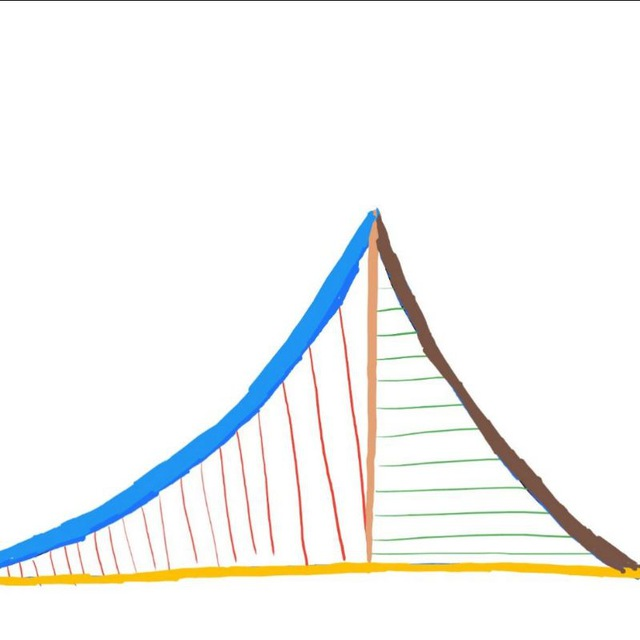
\includegraphics[width=0.3\columnwidth]{figs/logo.jpg}
\\
		{	\huge G. V. V. Sharma}
	\end{flushleft}
%\IEEEpubid{\makebox[\columnwidth]{978-1-7281-5966-1/20/\$31.00 ©2020 IEEE \hfill} \hspace{\columnsep}\makebox[\columnwidth]{ }}
}
\maketitle

\newpage
\section*{About this Book}

This book introduces matrices through high school coordinate geometry. This approach makes it easier for beginners to learn Python for scientific computing. All problems in the book are from NCERT mathematics textbooks from Class 9-12.   
The content is sufficient for industry jobs and covers nearly all matrix prerequisites for machine learning.
There is no copyright, so readers are free to print and share.  
\begin{flushright}
\today
\end{flushright}
Github: https://github.com/gadepall/matgeo
		\\
License: https://creativecommons.org/licenses/by-sa/3.0/
\\
and
\\
https://www.gnu.org/licenses/fdl-1.3.en.html
\\
First manual appeared in January 2018
\\
First edition published on July 10, 2024
\\
In this edition, some incorrect solutions were removed.  Many figures redrawn. More problems added.

\newpage


\tableofcontents

\newpage
%\twocolumn
\onecolumn


%\renewcommand{\theequation}{\theenumi}
\numberwithin{equation}{enumi}
\numberwithin{figure}{enumi}
%\renewcommand{\thefigure}{\theenumi}
\renewcommand{\thetable}{\theenumi}


\section{Vector Arithmetic}
\subsection{Formulae}
%\begin{enumerate}[label=\arabic*.,ref=\theenumi]
\begin{enumerate}[label=\thesubsection.\arabic*.,ref=\thesubsection.\theenumi]
\numberwithin{equation}{enumi}
	\item The {\em direction vector} of $AB$ is defined as
		\begin{align}
		\label{eq:dir-vec}
			\vec{m}=\vec{B}-
			\vec{A} = \kappa
			\myvec{1 \\ m}
		\end{align}
		where $m$ is the slope of $AB$.  We also say that 
\begin{align}
\vec{m}\equiv   \myvec{1 \\ m}
\end{align}
	\item The lines with direction vectors $\vec{m}_1$ and $\vec{m}_2$
		respectively, are parallel if 
\begin{align}
\vec{m}_1\equiv   \vec{m}_2
\end{align}
  \item If $ABCD$ be a parallelogram with $AB \parallel CD$,
	  \label{prop:two-pgm}
  \begin{align}
	  \label{eq:two-pgm}
 \vec{B}-\vec{A} = \vec{C} -\vec{D}
  \end{align}
\item If $\vec{D}$ divides $BC$ in the ratio $k : 1$,
		\begin{align}
			\vec{D}= \frac{k\vec{C}+\vec{B}}{k+1}
	  \label{eq:section_formula}
		\end{align}
  \item 
If $PQRS$ is formed by joining the mid points of $ABCD$, 
\begin{align}
  \vec{P} = \frac{1}{2}\brak{\vec{A}+\vec{B}} 
  ,\,
 \vec{Q} = \frac{1}{2}\brak{\vec{B}+\vec{C}} 
 \\
 \vec{R} = \frac{1}{2}\brak{\vec{C}+\vec{D}}   
  ,\,
 \vec{S} = \frac{1}{2}\brak{\vec{D}+\vec{A}}  
 \\
	\implies 
 \vec{P}-\vec{Q} = \vec{S} -\vec{R}.
  \label{eq:10/7/4/8det2f}
\end{align}
Hence, $PQRS$ is a parallelogram
	  from \eqref{eq:two-pgm}.
	\item In 2D space,  the basis vectors are defined as 
\begin{align}
	\vec{e}_1 = \myvec{1 \\ 0},\
	\vec{e}_2 = \myvec{0 \\ 1}.
\end{align}
	\item The length of a vector  is  defined as
		\begin{align}
		\label{eq:side-length}
			 \norm{\vec{x}} \triangleq \sqrt{\vec{x}^{\top}\vec{x}}
		\end{align}
		For example, if 
\begin{align}
\vec{x}
	&=\myvec{3 \\ 4},
	\\
	\vec{x}^{\top}\vec{x} &= \myvec{3 & 4}\myvec{3 \\ 4}
	\label{eq:scalar-product}
	\\
	&=3 \times 3 + 4 \times 4 = 25
\end{align}
yielding
		\begin{align}
			 \norm{\vec{x}} = 5.
		\end{align}
	\eqref{eq:scalar-product}
	is known as the scalar product.
	\item The unit vector in the direction of $\vec{x}$ is 
		\begin{align}
		\label{eq:unit-vec}
			 \frac{\vec{x}}{\norm{\vec{x}}} 
		\end{align}
		\iffalse
\item   For a 2D space, 
	points $\vec{A}, \vec{B}, \vec{C}$ are defined to be collinear if 
		\fi
	\item 
	Points $\vec{A}, \vec{B}, \vec{C}$ are defined to be collinear if 
		\begin{align}
			\label{eq:line-rank-2}
			\rank{\myvec{\vec{B}-\vec{A}& \vec{C}-\vec{A}}} = 1
		\end{align}
	\item 
\begin{align}
			\label{eq:mat-rank-t}
	\rank{\vec{A}}
	=
	\rank{\vec{A}^\top}
\end{align}
\item In the 2D space, the unit direction vector is defined as
\begin{align}
		\label{eq:dir-vec-3d}
\vec{m}=\myvec{\cos \alpha\\ \cos \beta }
\end{align}
where ${ \alpha,  \beta }$ are the angles made by the vector with the axes.
\end{enumerate}

\subsection{Point Vectors}
\begin{enumerate}[label=\thesubsection.\arabic*, ref=\thesubsection.\theenumi]
	\item 		Find the values of $x$ and $y$ so that the vectors
$2\hat{i}+3\hat{j}$
and 
$x\hat{i}+y\hat{j}$
are equal.
\\
\solution
From the given informatin, 
\begin{align}
	\myvec{2\\3} = \myvec{x \\ y} 
	\\
	\implies x = 2, y = 3
\end{align}

\item Find the values of $x, y, z$ so that the vectors 
$x\hat{i}+2\hat{j}+z\hat{k}$
and 
$2\hat{i}+y\hat{j}+\hat{k}$
are equal.
\item Find the sum of the vectors $\vec{a}=\hat{i}-2\hat{j}+\hat{k}$,  $\vec{b}=-2\hat{i}+4\hat{j}+5\hat{k}$ and $\vec{c}=\hat{i}-6\hat{j}-7\hat{k}$.
\item Find the slope of a line,  which passes through the origin and the mid point of the line segment joining the points $\vec{P}$(0, -4) and $\vec{B}$(8, 0).
\label{chapters/11/10/1/5}
	\\
	\solution
The mid point of $PB$ is
\begin{align}
\vec{M} =\frac{1}{2}(\vec{P}+\vec{B})
	= \myvec{4 \\ -2}  
\end{align}
which, from  \eqref{eq:dir-vec}, is equal to the direction vector of $OM$, where $\vec{O}$ is the origin.
\begin{align}
\because \vec{M} \equiv
	 \myvec{1 \\ -\frac{1}{2}},
	m = -\frac{1}{2}
\end{align}
which, from \eqref{eq:dir-vec},  is the desired slope.
See 
		\figref{fig:11/10/1/5}.
	\begin{figure}[H]
		\centering
 %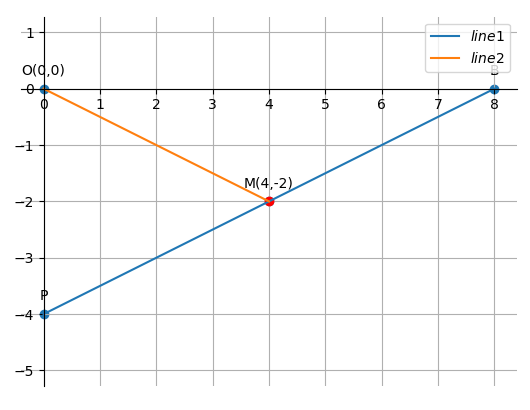
\includegraphics[width=0.75\columnwidth]{chapters/11/10/1/5/figs/line.png}
 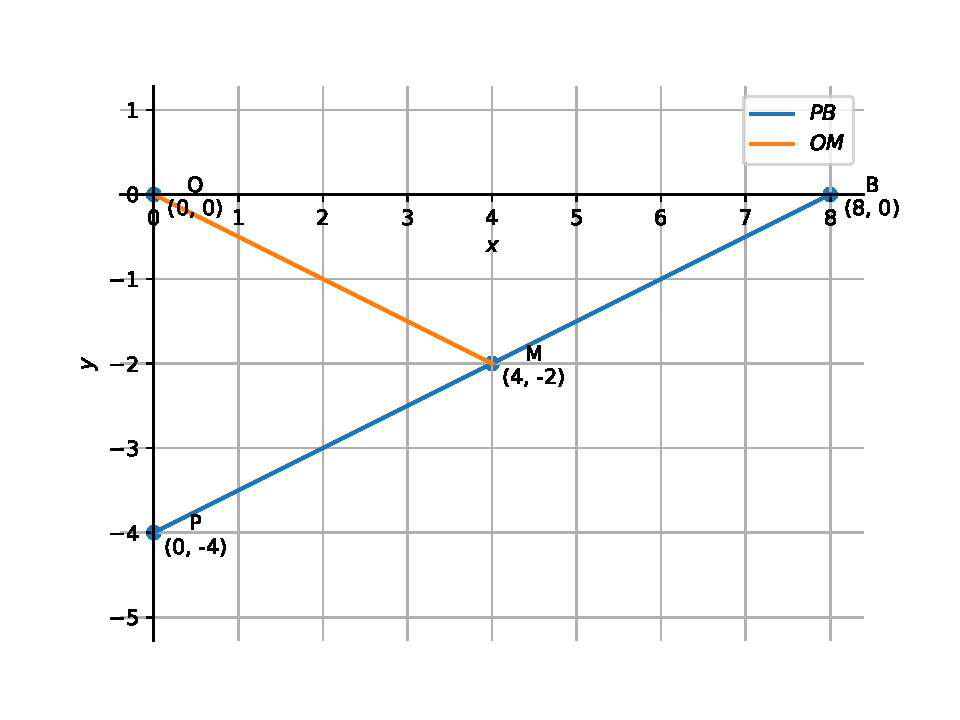
\includegraphics[width=0.75\columnwidth]{chapters/11/10/1/5/figs/fig.pdf}
		\caption{}
		\label{fig:11/10/1/5}
  	\end{figure}

\item Find the angle between x-axis and the line joining points (3, -1) and (4, -2).
\label{chapters/11/10/1/10}
\\
\solution 
The direction vector of the given line is 
\begin{align}
	\vec{C}
=\myvec{ -1\\ 1 }
\end{align}
Hence, the desired angle is given by
\begin{align}
	\cos\theta=\frac{\vec{C}^{\top}\vec{e}_1}{\norm{\vec{C}}\norm{\vec{e}_1}}
	&= -\frac{1}{\sqrt{2}}
	\\
	\implies 
	\theta&=135\degree
 \end{align}

\item A line passes through $\vec{A}(x_1, y_1)$ and $\vec{B}(h, k)$. If slope of the line is m,  show that $(k-y_1)=m(h-x_1)$.
\label{chapters/11/10/1/12}
\\
\solution 
The direction vector
\begin{align}
	\vec{B}-\vec{A}
	=
	\myvec{
  h-x_1\\
  k-y_1
  }
   \equiv
	\myvec{
1\\
	\frac{ k-y_1}{h-x_1}
  }
  \\
	\implies m = 
	\frac{ k-y_1}{h-x_1},
\end{align}
yielding the desired result.

\item
Show that the line through the points \brak{4, 7, 8}, \brak{2, 3, 4} is parallel to the line through the points \brak{-1, -2, 1}, \brak{1, 2, 5}.
	\label{12.11.2.3}
\\
\solution
	Show that the line through the points \brak{4,7,8},\brak{2,3,4} is parallel to the line through the points\brak{-1,-2,1},\brak{1,2,5}.

\textbf{Solution :}
For line passing through \brak{4,7,8},\brak{2,3,4},the direction vector,\begin{align}
    \vec{m_1}&=\myvec{-2\\-4\\-4}
\end{align}
For line passing through \brak{-1,-2,1},\brak{1,2,5},the direction vector,\begin{align}
    \vec{m_2}&=\myvec{2\\4\\4}
\end{align}
Therefore,the lines are parallel to each other.

\item The vector having intial and terminal points as (-2, 5, 0) and (3, 7, 4), respectively is
\solution
The desired vector is
\begin{align}
	\myvec{3 \\ 7 \\ 4}
	-\myvec{-2 \\ 5 \\ 0} = 
	\myvec{5 \\ 2 \\ 4}  
\end{align}
\item Find the vector joining the points $\vec{P}\brak{2, 3, 0}$ and $\vec{Q}\brak{-1, -2, -4}$ directed from $\vec{P}$ to $\vec{Q}$.
\item Without using distance formula,  show that points $\vec{A}(– 2,  – 1),  \vec{B}(4,  0),  \vec{C}(3,  3)$ and $\vec{D}(–3,  2)$ are the vertices of a parallelogram.
\label{chapters/11/10/1/9}
\\
\solution
	  From \eqref{eq:two-pgm},
\begin{align}
\vec{A}-\vec{B} = 
\vec{D}-\vec{C} =  \myvec{-6\\-1}
\end{align}
Hence, $ABCD$ is a parallelogram.
See \figref{fig:chapters/11/10/1/91}.
\begin{figure}[h!]
  \centering
   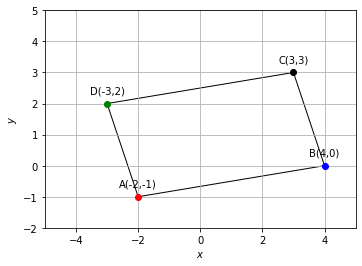
\includegraphics[width=\columnwidth]{chapters/11/10/1/9/figs/paralellogram.png}
    \caption{}
     \label{fig:chapters/11/10/1/91}  
\end{figure}




\item If the points $\vec{A}(6,  1),  \vec{B}(8,  2),  \vec{C}(9,  4)$ and $\vec{D}(p,  3)$ are the vertices of a parallelogram,  taken in order,  find the value of $p$.
\label{10/7/0/10}
\item 
If $(1,  2),  (4,  y),  (x,  6)$ and $(3,  5)$ are the vertices of a parallelogram taken in order,  find $x$ and $y$.
\label{10/7/2/6}
\item The fourth vertex $\vec{D}$ of a parallelogram $ABCD$ whose three vertices are
	$\vec{A} (–2,  3),  \vec{B} (6,  7)$ and  $\vec{C} (8,  3)$ is
\item Verify if the points $\vec{A}(4, 3),  \vec{B}(6, 4), \vec{C}(5, -6)$  and  $\vec{D}(-3, 5)$ are the vertices of a parallelogram.
\item A girl walks 4 km towards west,  then she walks 3 km in a direction 30$^{\circ}$ east of north and stops. Determine the girl's displacement from her initial point of departure.\\
	\solution
		See  
\figref{fig:chapters/12/10/5/3Fig1}.
Let the initial position
be
\begin{align}
	\vec{A}=\myvec{0\\0}
\end{align}
After going west, the position becomes
\begin{align}
			\vec{B}=\myvec{-4\\0}
\end{align}
If the final position be $\vec{C}$, from the given information,
\begin{align}
	 \vec{C}-\vec{B}=3\myvec{\cos{60\degree}\\\sin{60\degree}}
	 \implies 
	\vec{C}  
=\myvec{\frac{-5}{2}\\[2pt] \frac{3\sqrt{3}}{2}}
\end{align}
which is the desired displacement. 
\begin{figure}[H] 
 \begin{center} 
 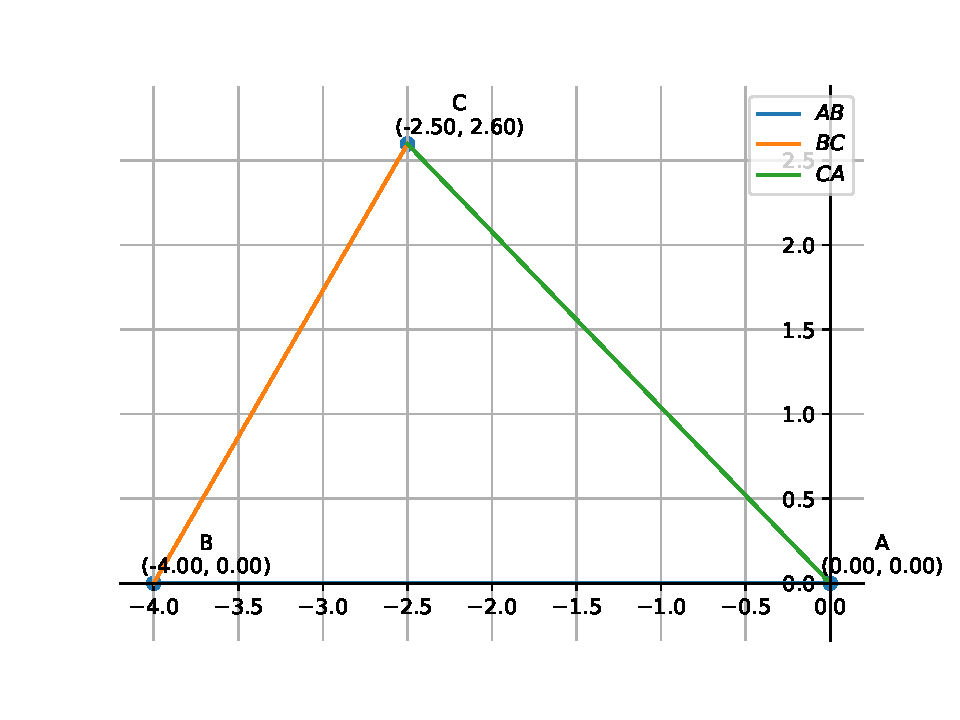
\includegraphics[width=0.75\columnwidth]{chapters/12/10/5/3/figs/fig.pdf} 
 \end{center} 
\caption{} 
\label{fig:chapters/12/10/5/3Fig1} 
\end{figure}

\item $(-1, 2, 1),  (1, -2, 5),  (4, -7, 8)$ and $(2, -3, 4)$ are the vertices of a parallelogram.
\item Three vertices of a parallelogram $ABCD$ are $\vec{A}(3, -1, 2),  \vec{B}(1, -2, 4)$ and $\vec{C}(-1, 1, 2)$. Find the coordinates of the fourth vertex.
\item If the origin is the centroid of the triangle $PQR$ with vertices $\vec{P}(2a, 2, 6),  \vec{Q}(-4, 3b, -10)$ and $R(8, 14, 2c)$,  then find the values of $a,  b$ and $c$.
\item Find the slope of lines
\begin{enumerate}
\item  Passing through the points $(3, -2)$ and $(-1, 4)$
\item  Passing through the points $(3, -2)$ and $(7, -2)$
\item  passing through the points $(3, -2)$ and $(3, 4)$	
\item  Making inclination of $60\degree$ with the positive direction of x-axis.
\end{enumerate}
\item The centroid of a triangle $ABC$ is at the point $(1, 1, 1)$. If the coordinates of $\vec{A}$ and $\vec{B}$ are $(3, -5, 7)$ and $(-1, 7, -6)$,  respectively find the coordinates of the point $\vec{C}$.
\item Represent graphically a displacement of $40$ km,  $30\degree$ west of south.
	\item Rain is falling vertically with a speed of 35 $m s^{-1}$
. Winds starts blowing after sometime with a speed of 12 $m s^{-1}$ in
east to west direction. In which direction should a boy waiting at a bus stop hold his umbrella ?
%
\item A motorboat is racing towards north at 25 km/h and the water current in that region is 10 km/h in the direction of 60$\degree$ east of south. Find the resultant velocity of the boat.
\item Rain is falling vertically with a speed of 35 $m s^{-1}$
. A woman rides a bicycle with a speed of 12 $ms^{-1}$ in east to west
direction. What is the direction in which she should hold her umbrella ?
\item Rain is falling vertically with a speed of 30 $m s^{-1}$. A woman rides a bicycle with a speed  of 10 $m s^{-1}$ in the north to south direction. What is the direction in which she should
hold her umbrella?
\item A man can swim with a speed of 4.0 km/h in still water. How long does he take to cross a river 1.0 km wide if the river flows steadily at 3.0 km/h and he makes his strokes normal to the river current? How far down the river does he go when he reaches the other bank ?
\item In a harbour,  wind is blowing at the speed of 72 km/h and the flag on the mast of a boat anchored in the harbour flutters along the N-E direction. If the boat starts moving at a speed of 51 km/h to the north,  what is the direction of the flag on the mast of the boat ?

\end{enumerate}

\subsection{CBSE}
\begin{enumerate}[label=\thesubsection.\arabic*, ref=\thesubsection.\theenumi]
    \item If in $\triangle ABC$, $\overrightarrow{BA} = 2\vec{a}$ and $\overrightarrow{BC} = 3\vec{b}$, then $\overrightarrow{AC}$ is
    \hfill (12, 2023)
	\item The coordinates of the three consecutive vertices of a parallelogram $ABCD$ are $\vec{\vec{A}}(1, 3)$, $\vec{B}(-1, 2)$, and $\vec{C}(2, 5)$. Find the coordinates of the fourth vertex $\vec{D}$. \hfill (10, 2021)
\item Points $\vec{A}(3, 1)$, $\vec{B}(5, 1)$, $\vec{C}(a, b)$, and $\vec{D}(4, 3)$ are vertices of a parallelogram $ABCD$. Find the values of $a$ and $b$. \hfill (10, 2019)
\item If $\vec{a}=2\hat{i}+3\hat{j}+\hat{k}$, $\vec{b}=\hat{i}-2\hat{j}+\hat{k}$ and $\vec{c}=-3\hat{i}+\hat{j}+2\hat{k}$, find $\myvec{\vec{a}&\vec{b}&\vec{c} }$
\hfill (12, 2018) 
\item If $\vec{A}\brak{1,3}$, $\vec{B}\brak{-1,2}$, $\vec{C}\brak{2,5}$ and $\vec{D}\brak{x,4}$ are the vertices of a parallelogram $ABCD$, then the value of $x$ is
\hfill (10, 2012)
    \item If $(3,3),(6,y),(x,7)$ and $(5,6)$ are the vertices of a parallelogram taken in order, find the values of $x$ and $y$.
\hfill (10, 2011)
	
\end{enumerate}

\subsection{Section Formula}
\begin{enumerate}[label=\thesubsection.\arabic*,ref=\thesubsection.\theenumi]

\item Find the coordinates of the point which divides the join of $(-1,7) \text{ and } (4,-3)$ in the ratio 2:3.
	\\
		\solution
	Using section formula \eqref{eq:section_formula}, the desired point is
\begin{align}
\frac{1}{1+\frac{3}{2}}  \myvec{\myvec{
4\\
-3
}
  +
   \frac{3}{2}\myvec{
-1\\
7
}}
=\myvec{
1\\
3
}
\end{align}
See 
\figref{fig:chapters/10/7/2/1/Fig}
\begin{figure}[H]
\begin{center}
   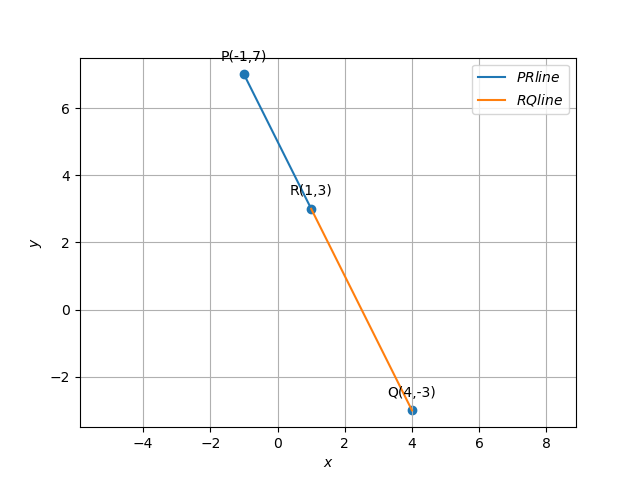
\includegraphics[width=0.75\columnwidth]{chapters/10/7/2/1/figs/linefig.png}
\end{center}
\caption{}
\label{fig:chapters/10/7/2/1/Fig}
\end{figure}


\item Find the coordinates of the points of trisection of the line segment joining $(4,-1)$  and  $(-2,3)$.
	\\
		\solution
	Using section formula,
\begin{align}
\vec{R}=\frac{1}{1+\frac{1}{2}}\brak{\myvec{4\\-1}+\frac{1}{2}\myvec{-2\\-3}}
=\myvec{2\\ \frac{-5}{3}}\\
\vec{S}=\frac{1}{1+\frac{2}{1}}\brak{\myvec{4\\-1}+\frac{2}{1}\myvec{-2\\-3}}
=\myvec{0\\ \frac{-7}{3}}
\end{align}
which are the desired points of trisection.
\iffalse
See
		\figref{fig:chapters/10/7/2/2/Figure}
\begin{figure}[H]
\centering
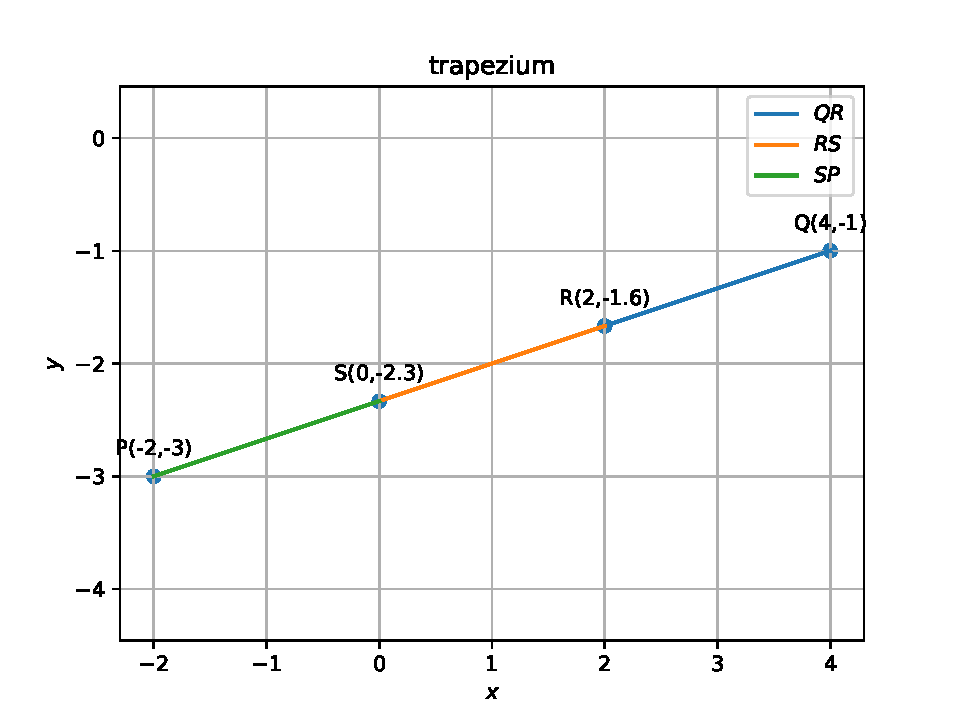
\includegraphics[width=0.75\columnwidth]{chapters/10/7/2/2/figs/dj.pdf}
\caption{}
		\label{fig:chapters/10/7/2/2/Figure}
\end{figure}
\fi

\item Find the ratio in which the line segment joining the points $(-3,10) \text{ and } (6,-8)$ $\text{ is divided by } (-1,6)$.
	\\
		\solution
	\iffalse
\documentclass[12pt]{article}
\usepackage{graphicx}
%\documentclass[journal,12pt,twocolumn]{IEEEtran}
\usepackage[none]{hyphenat}
\usepackage{graphicx}
\usepackage{listings}
\usepackage[english]{babel}
\usepackage{graphicx}
\usepackage{caption} 
\usepackage{hyperref}
\usepackage{booktabs}
\def\inputGnumericTable{}
\usepackage{color}                                            %%
    \usepackage{array}                                            %%
    \usepackage{longtable}                                        %%
    \usepackage{calc}                                             %%
    \usepackage{multirow}                                         %%
    \usepackage{hhline}                                           %%
    \usepackage{ifthen}
\usepackage{array}
\usepackage{amsmath}   % for having text in math mode
\usepackage{listings}
\lstset{
language=tex,
frame=single, 
breaklines=true
}
  
%Following 2 lines were added to remove the blank page at the beginning
\usepackage{atbegshi}% http://ctan.org/pkg/atbegshi
\AtBeginDocument{\AtBeginShipoutNext{\AtBeginShipoutDiscard}}
%
%New macro definitions
\newcommand{\mydet}[1]{\ensuremath{\begin{vmatrix}#1\end{vmatrix}}}
\providecommand{\brak}[1]{\ensuremath{\left(#1\right)}}
\providecommand{\norm}[1]{\left\lVert#1\right\rVert}
\newcommand{\solution}{\noindent \textbf{Solution: }}
\newcommand{\myvec}[1]{\ensuremath{\begin{pmatrix}#1\end{pmatrix}}}
\let\vec\mathbf
\begin{document}
\begin{center}
\title{\textbf{Coordinate Geometry}}
\date{\vspace{-5ex}} %Not to print date automatically
\maketitle
\end{center}
\setcounter{page}{1}
\section*{10$^{th}$ Maths - Chapter 7}
This is Problem-4 from Exercise 7.2
\begin{enumerate}
\item Find the ratio in which the line segement joining the points $\myvec{-3 \\ 10}$ and $\myvec{6\\-8}$ is divided by $\myvec{-1\\6}$.\\
\solution \\
\fi
		The input parameters for this problem are available in Table \eqref{tab:10/7/2/4-1}.
\begin{table}[ht!]
%%%%%%%%%%%%%%%%%%%%%%%%%%%%%%%%%%%%%%%%%%%%%%%%%%%%%%%%%%%%%%%%%%%%%%
%%                                                                  %%
%%  This is the header of a LaTeX2e file exported from Gnumeric.    %%
%%                                                                  %%
%%  This file can be compiled as it stands or included in another   %%
%%  LaTeX document. The table is based on the longtable package so  %%
%%  the longtable options (headers, footers...) can be set in the   %%
%%  preamble section below (see PRAMBLE).                           %%
%%                                                                  %%
%%  To include the file in another, the following two lines must be %%
%%  in the including file:                                          %%
%%        \def\inputGnumericTable{}                                 %%
%%  at the beginning of the file and:                               %%
%%        \input{name-of-this-file.tex}                             %%
%%  where the table is to be placed. Note also that the including   %%
%%  file must use the following packages for the table to be        %%
%%  rendered correctly:                                             %%
%%    \usepackage[latin1]{inputenc}                                 %%
%%    \usepackage{color}                                            %%
%%    \usepackage{array}                                            %%
%%    \usepackage{longtable}                                        %%
%%    \usepackage{calc}                                             %%
%%    \usepackage{multirow}                                         %%
%%    \usepackage{hhline}                                           %%
%%    \usepackage{ifthen}                                           %%
%%  optionally (for landscape tables embedded in another document): %%
%%    \usepackage{lscape}                                           %%
%%                                                                  %%
%%%%%%%%%%%%%%%%%%%%%%%%%%%%%%%%%%%%%%%%%%%%%%%%%%%%%%%%%%%%%%%%%%%%%%



%%  This section checks if we are begin input into another file or  %%
%%  the file will be compiled alone. First use a macro taken from   %%
%%  the TeXbook ex 7.7 (suggestion of Han-Wen Nienhuys).            %%
\def\ifundefined#1{\expandafter\ifx\csname#1\endcsname\relax}


%%  Check for the \def token for inputed files. If it is not        %%
%%  defined, the file will be processed as a standalone and the     %%
%%  preamble will be used.                                          %%
\ifundefined{inputGnumericTable}

%%  We must be able to close or not the document at the end.        %%
 \def\gnumericTableEnd{\end{document}}


%%%%%%%%%%%%%%%%%%%%%%%%%%%%%%%%%%%%%%%%%%%%%%%%%%%%%%%%%%%%%%%%%%%%%%
%%                                                                  %%
%%  This is the PREAMBLE. Change these values to get the right      %%
%%  paper size and other niceties.                                  %%
%%                                                                  %%
%%%%%%%%%%%%%%%%%%%%%%%%%%%%%%%%%%%%%%%%%%%%%%%%%%%%%%%%%%%%%%%%%%%%%%

 \documentclass[12pt%
     %,landscape%
                    ]{report}
       \usepackage[latin1]{inputenc}
       \usepackage{fullpage}
       \usepackage{color}
       \usepackage{array}
       \usepackage{longtable}
       \usepackage{calc}
       \usepackage{multirow}
       \usepackage{hhline}
       \usepackage{ifthen}

 \begin{document}


%%  End of the preamble for the standalone. The next section is for %%
%%  documents which are included into other LaTeX2e files.          %%
\else

%%  We are not a stand alone document. For a regular table, we will %%
%%  have no preamble and only define the closing to mean nothing.   %%
    \def\gnumericTableEnd{}

%%  If we want landscape mode in an embedded document, comment out  %%
%%  the line above and uncomment the two below. The table will      %%
%%  begin on a new page and run in landscape mode.                  %%
%       \def\gnumericTableEnd{\end{landscape}}
%       \begin{landscape}


%%  End f theoelse clause for this file being \input.              %%
\fi

%%%%%%%%%%%%%%%%%%%%%%%%%%%%%%%%%%%%%%%%%%%%%%%%%%%%%%%%%%%%%%%%%%%%%%
%%                                                                  %%
%%  The rest is the gnumeric table, except for the closing          %%
%%  statement. Changes below will alter the table's appearance.     %%
%%                                                                  %%
%%%%%%%%%%%%%%%%%%%%%%%%%%%%%%%%%%%%%%%%%%%%%%%%%%%%%%%%%%%%%%%%%%%%%%

\providecommand{\gnumericmathit}[1]{#1} 
%%  Uncomment the next line if you would like your numbers to be in %%
%%  italics if they are italizised in the gnumeric table.           %%
%\renewcommand{\gnumericmathit}[1]{\mathit{#1}}
\providecommand{\gnumericPB}[1]%
{\let\gnumericTemp=\\#1\let\\=\gnumericTemp\hspace{0pt}}
 \ifundefined{gnumericTableWidthDefined}
        \newlength{\gnumericTableWidth}
        \newlength{\gnumericTableWidthComplete}
        \newlength{\gnumericMultiRowLength}
        \global\def\gnumericTableWidthDefined{}
 \fi
%% The following setting protects this code from babel shorthands.  %%
 \ifthenelse{\isundefined{\languageshorthands}}{}{\languageshorthands{english}}
%%  The default table format retains the relative column widths of  %%
%%  gnumeric. They can easily be changed to c, r or l. In that case %%
%%  you may want to comment out the next line and uncomment the one %%
%%  thereafter                                                      %%
\providecommand\gnumbox{\makebox[0pt]}
%%\providecommand\gnumbox[1][]{\makebox}

%% to adjust positions in multirow situations                       %%
\setlength{\bigstrutjot}{\jot}
\setlength{\extrarowheight}{\doublerulesep}

%%  The \setlongtables command keeps column widths the same across  %%
%%  pages. Simply comment out next line for varying column widths.  %%
\setlongtables

\setlength\gnumericTableWidth{%
 53pt+%
 53pt+%
 82pt+%
 53pt+%
0pt}
\def\gumericNumCols{4}
\setlength\gnumericTableWidthComplete{\gnumericTableWidth+%
         \tabcolsep*\gumericNumCols*2+\arrayrulewidth*\gumericNumCols}
\ifthenelse{\lengthtest{\gnumericTableWidthComplete > \linewidth}}%
         {\def\gnumericScale{1*\ratio{\linewidth-%
                        \tabcolsep*\gumericNumCols*2-%
                        \arrayrulewidth*\gumericNumCols}%
{\gnumericTableWidth}}}%
{\def\gnumericScale{1}}

%%%%%%%%%%%%%%%%%%%%%%%%%%%%%%%%%%%%%%%%%%%%%%%%%%%%%%%%%%%%%%%%%%%%%%
%%                                                                  %%
%% The following are the widths of the various columns. We are      %%
%% defining them here because then they are easier to change.       %%
%% Depending on the cell formats we may use them more than once.    %%
%%                                                                  %%
%%%%%%%%%%%%%%%%%%%%%%%%%%%%%%%%%%%%%%%%%%%%%%%%%%%%%%%%%%%%%%%%%%%%%%

\ifthenelse{\isundefined{\gnumericColA}}{\newlength{\gnumericColA}}{}\settowidth{\gnumericColA}{\begin{tabular}{@{}p{53pt*\gnumericScale}@{}}x\end{tabular}}
\ifthenelse{\isundefined{\gnumericColB}}{\newlength{\gnumericColB}}{}\settowidth{\gnumericColB}{\begin{tabular}{@{}p{53pt*\gnumericScale}@{}}x\end{tabular}}
\ifthenelse{\isundefined{\gnumericColC}}{\newlength{\gnumericColC}}{}\settowidth{\gnumericColC}{\begin{tabular}{@{}p{82pt*\gnumericScale}@{}}x\end{tabular}}
\ifthenelse{\isundefined{\gnumericColD}}{\newlength{\gnumericColD}}{}\settowidth{\gnumericColD}{\begin{tabular}{@{}p{53pt*\gnumericScale}@{}}x\end{tabular}}

\begin{center}
\begin{tabular}[c]{%
 b{\gnumericColA}%
 b{\gnumericColB}%
 b{\gnumericColC}%
 b{\gnumericColD}%
 }

%%%%%%%%%%%%%%%%%%%%%%%%%%%%%%%%%%%%%%%%%%%%%%%%%%%%%%%%%%%%%%%%%%%%%%
%%  The longtable options. (Caption, headers... see Goosens, p.124) %%
% \caption{The Table Caption.}             \\ %
% \hline % Across the top of the table.
%%  The rest of these options are table rows which are placed on    %%
%%  the first, last or every page. Use \multicolumn if you want.    %%

%%  Header for the first page.                                      %%
% \multicolumn{4}{c}{The First Header} \\ \hline 
% \multicolumn{1}{c}{colTag} %Column 1
% &\multicolumn{1}{c}{colTag} %Column 2
% &\multicolumn{1}{c}{colTag} %Column 3
% &\multicolumn{1}{c}{colTag} \\ \hline %Last column
% \endfirsthead

%%  The running header definition.                                  %%
% \hline
% \multicolumn{4}{l}{\ldots\small\slshape continued} \\ \hline
% \multicolumn{1}{c}{colTag} %Column 1
% &\multicolumn{1}{c}{colTag} %Column 2
% &\multicolumn{1}{c}{colTag} %Column 3
% &\multicolumn{1}{c}{colTag} \\ \hline %Last column
% \endhead

%%  The running footer definition.                                  %%
% \hline
% \multicolumn{4}{r}{\small\slshape continued\ldots} \\
% \endfoot

%%  The ending footer definition.                                   %%
% \multicolumn{4}{c}{That's all folks} \\ \hline 
% \endlastfoot
%%%%%%%%%%%%%%%%%%%%%%%%%%%%%%%%%%%%%%%%%%%%%%%%%%%%%%%%%%%%%%%%%%%%%%

\hhline{|-|-|-~}
  \multicolumn{1}{|p{\gnumericColA}|}%
 {\gnumericPB{\centering}\gnumbox{\textbf{Symbol}}}
 &\multicolumn{1}{p{\gnumericColB}|}%
 {\gnumericPB{\centering}\gnumbox{\textbf{Value}}}
 &\multicolumn{1}{p{\gnumericColC}|}%
 {\gnumericPB{\centering}\gnumbox{\textbf{Description}}}
 &
\\
\hhline{|---|~}
  \multicolumn{1}{|p{\gnumericColA}|}%
 {\gnumericPB{\centering}\gnumbox{$\vec{P}$}}
 &\multicolumn{1}{p{\gnumericColB}|}%
 {\gnumericPB{\centering}\gnumbox{$\myvec{-3\\10}$}}
 &\multicolumn{1}{p{\gnumericColC}|}%
 {\gnumericPB{\centering}\gnumbox{First point}}
 &
\\
\hhline{|---|~}
  \multicolumn{1}{|p{\gnumericColA}|}%
 {\gnumericPB{\centering}\gnumbox{$\vec{Q}$}}
 &\multicolumn{1}{p{\gnumericColB}|}%
 {\gnumericPB{\centering}\gnumbox{$\myvec{6\\-8}$}}
 &\multicolumn{1}{p{\gnumericColC}|}%
 {\gnumericPB{\centering}\gnumbox{Second point}}
 &
\\
\hhline{|---|~}
  \multicolumn{1}{|p{\gnumericColA}|}%
 {\gnumericPB{\centering}\gnumbox{$\vec{R}$}}
 &\multicolumn{1}{p{\gnumericColB}|}%
 {\gnumericPB{\centering}\gnumbox{$\myvec{-1\\6}$}}
 &\multicolumn{1}{p{\gnumericColC}|}%
 {\gnumericPB{\centering}\gnumbox{Desired point}}
 &
\\
\hhline{|-|-|-|~}
\end{tabular}
 \end{center}

\ifthenelse{\isundefined{\languageshorthands}}{}{\languageshorthands{\languagename}}
\gnumericTableEnd

\caption{}
\label{tab:10/7/2/4-1} 
\end{table}
Using section formula,
\begin{align}
         \vec{R} &=\frac{\vec{Q}+n\vec{P}}{1+n}\label{eq:chapters/10/7/2/4/1}
\end{align}
Substituting the values of $\vec{P},\vec{Q}$ and $\vec{R}$ in \eqref{eq:chapters/10/7/2/4/1}
\begin{align}
         \myvec{-1\\6} &=\frac{{\myvec{-3\\10}+n\myvec{6\\-8}}}{1+n}\\
 &=\frac{1}{1+n}\brak{{\myvec{-3\\10}+n\myvec{6\\-8}}} \\
 &=\frac{1}{1+n}\myvec{-3+6n\\10-8n} \label{eq:chapters/10/7/2/4/4}
\end{align}
Simplifying \eqref{eq:chapters/10/7/2/4/4} yeilds,
\begin{align}
          -1 &=\frac{-3+6n}{1+n}\\
\implies          n &=\frac{2}{7}
\end{align}
Also,
\begin{align}
          6 &=\frac{10-8n}{1+n}\\
    \implies      n &=\frac{2}{7}
\end{align}
Hence the desired ratio is $\dfrac{2}{7}$.  
\begin{figure}[!h]
 \begin{center}
  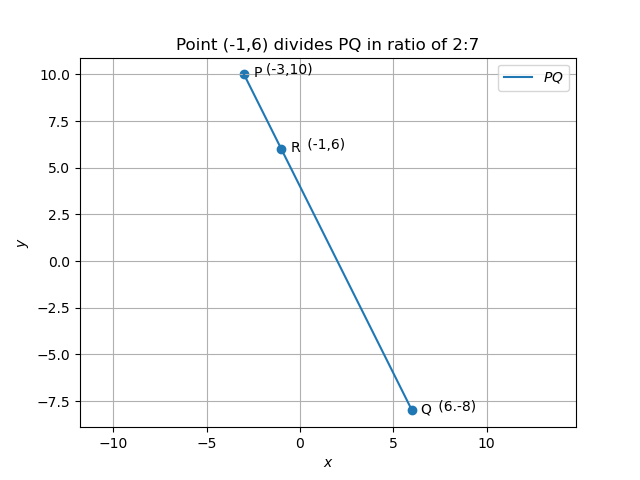
\includegraphics[width=\columnwidth]{chapters/10/7/2/4/figs/fig.png}
 \end{center}
\caption{}
\label{fig:10/7/2/4Fig1}
\end{figure}

\item Find the coordinates of a point $A$, where $AB$ is the diameter of a circle whose centre is $ C(2,-3)$  and  $B$ is $(1,4)$.
	\\
		\solution
		\begin{align}
	\vec{C} = \frac{\vec{A+B}}{2} 
	\implies 	\vec{A} = 2\vec{C}-\vec{B} 
	 = \myvec{3\\-10\\}	
	\end{align}       
	The radius is then obtained as
\begin{align}
	\norm{\vec{B}-\vec{C}} = 5\sqrt{2}
\end{align}
	See 
\figref{fig:chapters/10/7/2/7Fig}.
\begin{figure}[H]
\begin{center}	
	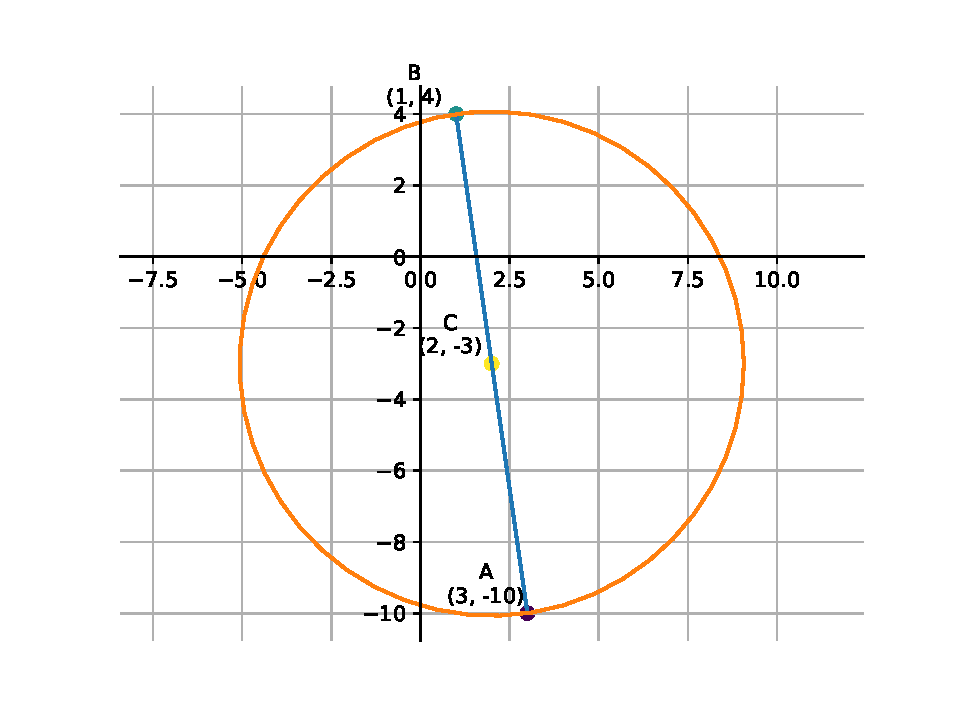
\includegraphics[width=0.75\columnwidth]{chapters/10/7/2/7/figs/fig.pdf}
\end{center}
\caption{}
\label{fig:chapters/10/7/2/7Fig}
\end{figure}
	

\item If $A$ and  $B$ are $(-2,-2)$ and  $(2,-4)$, respectively, find the coordinates of $P$ such that $AP= \frac {3}{7}AB$  and $ P$ lies on the line segment $AB$.
	\\
		\solution
	Using section formula, 
\begin{align}
\vec{P}&=\frac{1}{1+\frac{3}{4}}\brak{\myvec{-2\\-2}+\frac{3}{4}\myvec{2\\-4}}
=\myvec{\frac{-2}{7}\\[1pt] \frac{-20}{7}}
\end{align}
\iffalse
See 
   \figref{fig:chapters/10/7/2/8/vec.png}.
\begin{figure}
   \centering 
 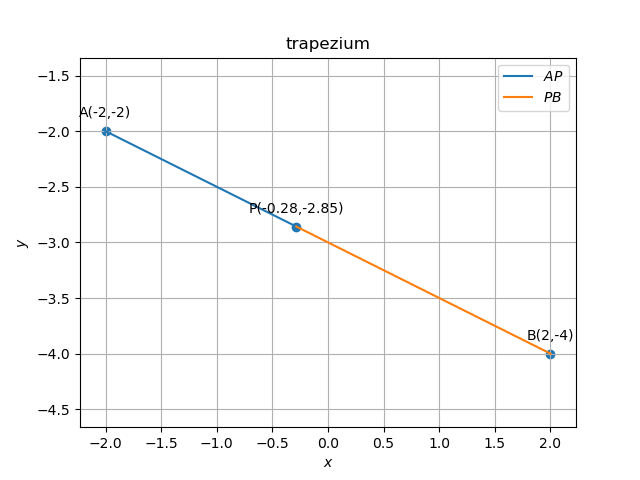
\includegraphics[width=0.75\columnwidth]{chapters/10/7/2/8/figs/vec.png}
   \caption{}
   \label{fig:chapters/10/7/2/8/vec.png}
   \end{figure}
   \fi

\item Find the coordinates of the points which divide the line segment joining $A(-2,2)$  and  $B(2,8)$ into four equal parts.
	\\
		\solution
	Using section formula,
\begin{align}
	\vec{R}_k=\frac{\vec{B}+k\vec{A}}{1+k}, k = \frac{i}{n-i}, 0 < i < n
\end{align}
for $n = 4$.
See 
\figref{fig:chapters/10/7/2/9/Fig}.
\begin{figure}[H]
\begin{center}
   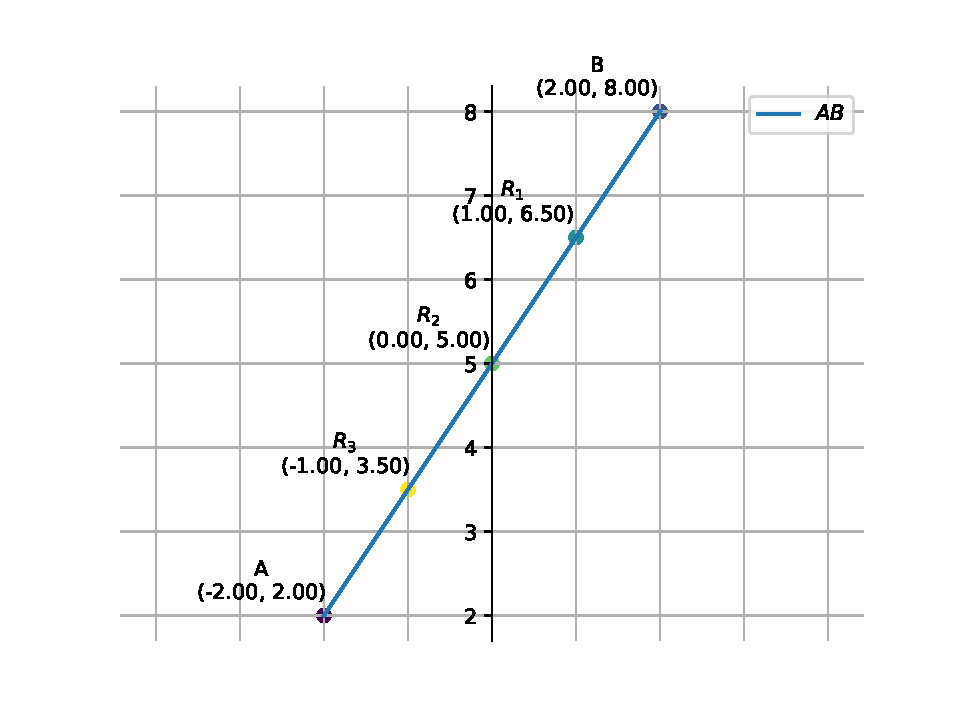
\includegraphics[width=0.75\columnwidth]{chapters/10/7/2/9/figs/fig.pdf}
\end{center}
\caption{}
\label{fig:chapters/10/7/2/9/Fig}
\end{figure}


\item Find the position vector of a point $\vec{R}$ which divides the line joining two points $\vec{P}$
and $\vec{Q}$ whose position vectors are $\hat{i}+2\hat{j}-\hat{k}$ and $-\hat{i}+\hat{j}+\hat{k}$ respectively, in the
ratio 2 : 1
\begin{enumerate}
    \item  internally
    \item  externally
\end{enumerate}
\solution
		\iffalse
\documentclass[journal,12pt,twocolumn]{IEEEtran}
%
\usepackage{setspace}
\usepackage{gensymb}
%\doublespacing
\singlespacing

%\usepackage{graphicx}
%\usepackage{amssymb}
%\usepackage{relsize}
\usepackage[cmex10]{amsmath}
%\usepackage{amsthm}
%\interdisplaylinepenalty=2500
%\savesymbol{iint}
%\usepackage{txfonts}
%\restoresymbol{TXF}{iint}
%\usepackage{wasysym}
\usepackage{amsthm}
%\usepackage{iithtlc}
\usepackage{mathrsfs}
\usepackage{txfonts}
\usepackage{stfloats}
\usepackage{bm}
\usepackage{cite}
\usepackage{cases}
\usepackage{subfig}
%\usepackage{xtab}
\usepackage{longtable}
\usepackage{multirow}
%\usepackage{algorithm}
%\usepackage{algpseudocode}
\usepackage{enumitem}
\usepackage{mathtools}
\usepackage{steinmetz}
\usepackage{tikz}
\usepackage{circuitikz}
\usepackage{verbatim}
\usepackage{tfrupee}
\usepackage[breaklinks=true]{hyperref}
%\usepackage{stmaryrd}
\usepackage{tkz-euclide} % loads  TikZ and tkz-base
%\usetkzobj{all}
\usetikzlibrary{calc,math}
\usepackage{listings}
    \usepackage{color}                                            %%
    \usepackage{array}                                            %%
    \usepackage{longtable}                                        %%
    \usepackage{calc}                                             %%
    \usepackage{multirow}                                         %%
    \usepackage{hhline}                                           %%
    \usepackage{ifthen}                                           %%
  %optionally (for landscape tables embedded in another document): %%
    \usepackage{lscape}     
\usepackage{multicol}
\usepackage{chngcntr}
%\usepackage{enumerate}
\usepackage{graphicx}

%\usepackage{wasysym}
%\newcounter{MYtempeqncnt}
\DeclareMathOperator*{\Res}{Res}
%\renewcommand{\baselinestretch}{2}
\renewcommand\thesection{\arabic{section}}
\renewcommand\thesubsection{\thesection.\arabic{subsection}}
\renewcommand\thesubsubsection{\thesubsection.\arabic{subsubsection}}

\renewcommand\thesectiondis{\arabic{section}}
\renewcommand\thesubsectiondis{\thesectiondis.\arabic{subsection}}
\renewcommand\thesubsubsectiondis{\thesubsectiondis.\arabic{subsubsection}}

% correct bad hyphenation here
\hyphenation{op-tical net-works semi-conduc-tor}
\def\inputGnumericTable{}                                 %%

\lstset{
%language=C,
frame=single, 
breaklines=true,
columns=fullflexible
}
%\lstset{
%language=tex,
%frame=single, 
%breaklines=true
%}

\begin{document}
%


\newtheorem{theorem}{Theorem}[section]
\newtheorem{problem}{Problem}
\newtheorem{proposition}{Proposition}[section]
\newtheorem{lemma}{Lemma}[section]
\newtheorem{corollary}[theorem]{Corollary}
\newtheorem{example}{Example}[section]
\newtheorem{definition}[problem]{Definition}
%\newtheorem{thm}{Theorem}[section] 
%\newtheorem{defn}[thm]{Definition}
%\newtheorem{algorithm}{Algorithm}[section]
%\newtheorem{cor}{Corollary}
\newcommand{\BEQA}{\begin{eqnarray}}
\newcommand{\EEQA}{\end{eqnarray}}
\newcommand{\define}{\stackrel{\triangle}{=}}

\bibliographystyle{IEEEtran}
%\bibliographystyle{ieeetr}


\providecommand{\mbf}{\mathbf}
\providecommand{\pr}[1]{\ensuremath{\Pr\left(#1\right)}}
\providecommand{\qfunc}[1]{\ensuremath{Q\left(#1\right)}}
\providecommand{\sbrak}[1]{\ensuremath{{}\left[#1\right]}}
\providecommand{\lsbrak}[1]{\ensuremath{{}\left[#1\right.}}
\providecommand{\rsbrak}[1]{\ensuremath{{}\left.#1\right]}}
\providecommand{\brak}[1]{\ensuremath{\left(#1\right)}}
\providecommand{\lbrak}[1]{\ensuremath{\left(#1\right.}}
\providecommand{\rbrak}[1]{\ensuremath{\left.#1\right)}}
\providecommand{\cbrak}[1]{\ensuremath{\left\{#1\right\}}}
\providecommand{\lcbrak}[1]{\ensuremath{\left\{#1\right.}}
\providecommand{\rcbrak}[1]{\ensuremath{\left.#1\right\}}}
\theoremstyle{remark}
\newtheorem{rem}{Remark}
\newcommand{\sgn}{\mathop{\mathrm{sgn}}}
\providecommand{\abs}[1]{\left\vert#1\right\vert}
\providecommand{\res}[1]{\Res\displaylimits_{#1}} 
\providecommand{\norm}[1]{\left\lVert#1\right\rVert}
%\providecommand{\norm}[1]{\lVert#1\rVert}
\providecommand{\mtx}[1]{\mathbf{#1}}
\providecommand{\mean}[1]{E\left[ #1 \right]}
\providecommand{\fourier}{\overset{\mathcal{F}}{ \rightleftharpoons}}
%\providecommand{\hilbert}{\overset{\mathcal{H}}{ \rightleftharpoons}}
\providecommand{\system}{\overset{\mathcal{H}}{ \longleftrightarrow}}
	%\newcommand{\solution}[2]{\textbf{Solution:}{#1}}
\newcommand{\solution}{\noindent \textbf{Solution: }}
\newcommand{\cosec}{\,\text{cosec}\,}
\providecommand{\dec}[2]{\ensuremath{\overset{#1}{\underset{#2}{\gtrless}}}}
\newcommand{\myvec}[1]{\ensuremath{\begin{pmatrix}#1\end{pmatrix}}}
\newcommand{\mydet}[1]{\ensuremath{\begin{vmatrix}#1\end{vmatrix}}}
%\numberwithin{equation}{section}
\numberwithin{equation}{subsection}
%\numberwithin{problem}{section}
%\numberwithin{definition}{section}
\makeatletter
\@addtoreset{figure}{problem}
\makeatother

\let\StandardTheFigure\thefigure
\let\vec\mathbf
%\renewcommand{\thefigure}{\theproblem.\arabic{figure}}
\renewcommand{\thefigure}{\theproblem}
%\setlist[enumerate,1]{before=\renewcommand\theequation{\theenumi.\arabic{equation}}
%\counterwithin{equation}{enumi}


%\renewcommand{\theequation}{\arabic{subsection}.\arabic{equation}}

\def\putbox#1#2#3{\makebox[0in][l]{\makebox[#1][l]{}\raisebox{\baselineskip}[0in][0in]{\raisebox{#2}[0in][0in]{#3}}}}
     \def\rightbox#1{\makebox[0in][r]{#1}}
     \def\centbox#1{\makebox[0in]{#1}}
     \def\topbox#1{\raisebox{-\baselineskip}[0in][0in]{#1}}
     \def\midbox#1{\raisebox{-0.5\baselineskip}[0in][0in]{#1}}

\vspace{3cm}

\title{EE2802: Assignment2}
\author{Nikam Pratik Balasaheb}





% make the title area
\maketitle

\newpage

%\tableofcontents

\bigskip

\renewcommand{\thefigure}{\theenumi}
\renewcommand{\thetable}{\theenumi}
%\renewcommand{\theequation}{\theenumi}

\section{Problem}
Find the position vector of a point R which divides the line joining two points P = $\myvec{1\\ 2 \\-1}$ and Q = $\myvec{ -1\\1\\1 }$ in the ratio 2:1 
\begin{enumerate}
\item internally
\item externally
\end{enumerate}

\section{Solution}

\begin{align}
\vec{P} = \myvec{ 1\\2\\-1} \\
 \vec{Q} = \myvec{ -1\\1\\1}
\end{align}

\fi

\begin{enumerate}


\item When $\vec{R}$ divides line segment joining $\vec{P}$ and $\vec{Q}$ internally,
\begin{align}
\vec{R} &= \frac{2 \vec{P} + 1 \vec{Q}}{3} \\
 &= \frac{2}{3} \vec{P} + \frac{1}{3} \vec{Q}\\
\vec{R} &= \myvec{\frac{1}{3}\\[1pt] \frac{5}{3} \\[1pt] \frac{-1}{3}}
\end{align}

\item When $\vec{R}$ divides line segment joining $\vec{P}$ and $\vec{Q}$ externally,
\begin{align}
\vec{R} &= 2 \vec{Q} - \vec{P} \\
 &= 2 \myvec{ -1\\1\\1} - \myvec{ 1\\2\\-1}\\
\vec{R} &= \myvec{ -3\\ 0 \\ 3 }
\end{align}


\end{enumerate}
See Fig. 
\ref{fig:chapters/12/10/2/15/}.
\begin{figure}[!ht]
\centering
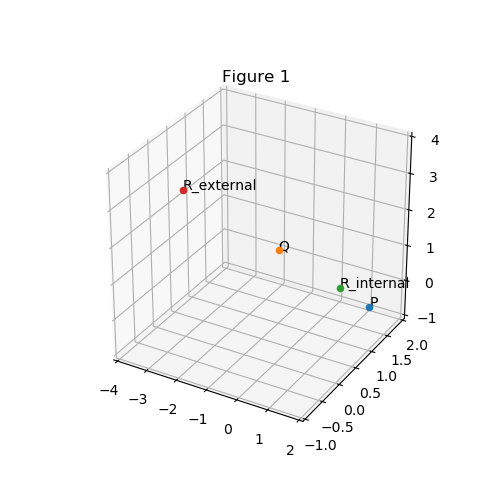
\includegraphics[width=\columnwidth]{chapters/12/10/2/15/figs/Figure_1.png}
\caption{}
\label{fig:chapters/12/10/2/15/}
\end{figure}



\item Find the position vector of the mid point of the vector joining the points $\vec{P}$(2, 3, 4)
and $\vec{Q}$(4, 1, –2).
\\
\solution
		The desired vector is
\begin{align}
\frac{1}{2}\myvec{2\\3\\4} +  \frac{1}{2}\myvec{4\\1\\-2} =\myvec{3\\2\\1} 
\end{align}




\item Determine the ratio in which the line $2x+y  - 4=0$ divides the line segment joining the points  $\vec{A}(2, - 2)$  and  $\vec{B}(3, 7)$.
\\
\solution
	\iffalse
\documentclass[journal,12pt,twocolumn]{IEEEtran}
\usepackage{graphicx}
\graphicspath{{./chapters/10/7/4/1/figs/}}{}
\usepackage{amsmath,amssymb,amsfonts,amsthm}
\newcommand{\myvec}[1]{\ensuremath{\begin{pmatrix}#1\end{pmatrix}}}
\providecommand{\norm}[1]{\lVert#1\rVert}
\usepackage{listings}
\usepackage{watermark}
\usepackage{titlesec}
\usepackage{caption}
\let\vec\mathbf
\lstset{
frame=single, 
breaklines=true,
columns=fullflexible
}
\thiswatermark{\centering \put(0,-105.0){
\includegraphics[scale=0.15]{/sdcard/IITH/vector/vectpr-4/chapters/10/7/4/1/figs/logo.png}} }
\title{\mytitle}
\title{
Assignment - Vector-4
}
\author{Surajit Sarkar}
\begin{document}
\maketitle
%\tableofcontents
\bigskip
\section{\textbf{Problem}}
Determine the ratio in which the line 2x+y–4=0 divides the line segment joining the points A(2,–2) and B(3,7).
\section{\textbf{Solution}}
\begin{table}[h]
    \centering
    \begin{tabular}{|c|c|}
       \hline
       \textbf{Symbol}&\textbf{Value}  \\
       \hline
	    $\vec{A}$ & $\myvec{2\\-2}$\\
        \hline
	    $\vec{B}$ & $\myvec{3\\7}$\\
        \hline
	    c&$4$\\
        \hline
       $\vec{n}$ & $\myvec{2\\1}$\\
       \hline
    \end{tabular}
    \caption{Parameters}
    \label{tab:my_label}
\end{table}
Given equation
\fi
The given equation can be expressed as
\begin{align}
    \myvec{2&1}\vec{x}&=4\\
\end{align}
Using section formula, the point of division 
\begin{align}
    \vec{P} = \frac{k\vec{B+A}}{k+1}
\end{align}
which upon substitution in the equation of a line yields
\begin{align}
    \implies\vec{n}^{\top}\myvec{\frac{k\vec{B+A}}{k+1}}&=c\\
    \implies k&=\frac{c-\vec{n}^{\top}\vec{A}}{\vec{n}^{\top}\vec{B}-c}\\
\end{align}
upon simplification.  Substituting numerical values, 
\begin{align}
    k=\frac{2}{9}
\end{align}
See Fig. 
\ref{fig:chapters/10/7/4/1vec}.
\begin{figure}[!h]
\centering
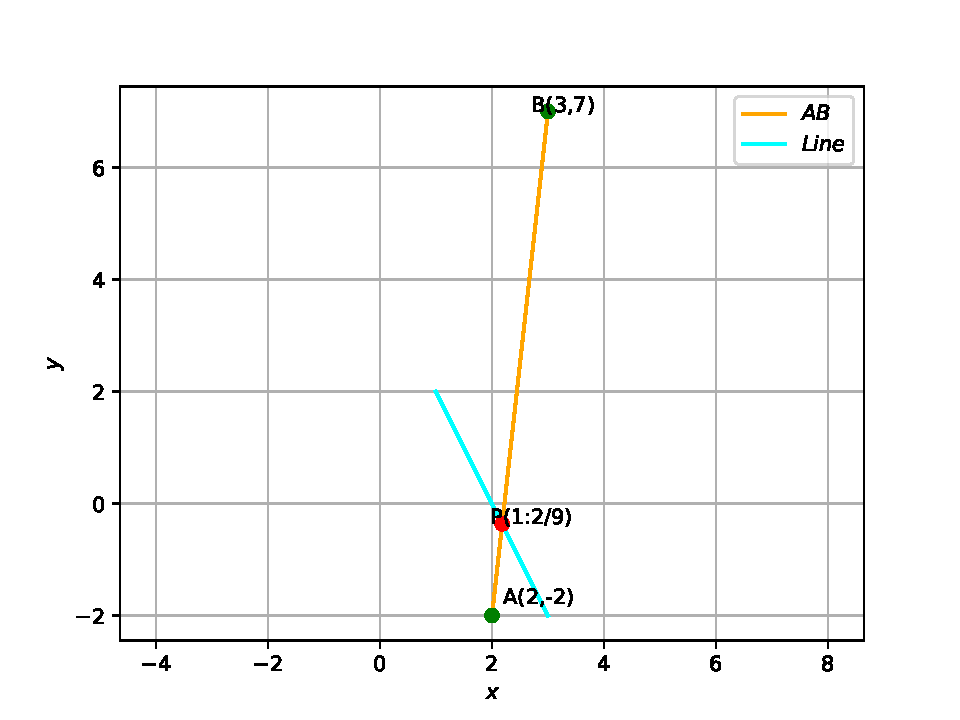
\includegraphics[width=\columnwidth]{chapters/10/7/4/1/figs/vec.pdf}
\caption{}
\label{fig:chapters/10/7/4/1vec}
\end{figure}


\item Let $\vec{A}(4, 2), \vec{B}(6, 5)$  and $ \vec{C}(1, 4)$ be the vertices of $\triangle ABC$.
\begin{enumerate}
\item The median from $\vec{A}$ meets $BC$ at $\vec{D}$. Find the coordinates of the point $\vec{D}$.
\item Find the coordinates of the point $\vec{P}$ on $AD$ such that $AP : PD = 2 : 1$.
\item Find the coordinates of points $\vec{Q}$ and $\vec{R}$ on medians $BE$ and $CF$ respectively such that $BQ : QE = 2 : 1$  and  $CR : RF = 2 : 1$.
\item What do you observe?
\item If $\vec{A}, \vec{B}$ and $\vec{C}$  are the vertices of $\triangle ABC$, find the coordinates of the centroid of the triangle.
\end{enumerate}
\solution
	\iffalse
\documentclass[12pt]{article}
\usepackage{graphicx}
\usepackage[none]{hyphenat}
\usepackage{graphicx}
\usepackage{listings}
\usepackage[english]{babel}
\usepackage{graphicx}
\usepackage{caption} 
\usepackage{booktabs}
\usepackage{array}
\usepackage{amssymb} % for \because
\usepackage{amsmath}   % for having text in math mode
\usepackage{extarrows} % for Row operations arrows
\usepackage{listings}
\usepackage[utf8]{inputenc}
\lstset{
  frame=single,
  breaklines=true
}
\usepackage{hyperref}
  
%Following 2 lines were added to remove the blank page at the beginning
\usepackage{atbegshi}% http://ctan.org/pkg/atbegshi
\AtBeginDocument{\AtBeginShipoutNext{\AtBeginShipoutDiscard}}


%New macro definitions
\newcommand{\mydet}[1]{\ensuremath{\begin{vmatrix}#1\end{vmatrix}}}
\providecommand{\brak}[1]{\ensuremath{\left(#1\right)}}
\newcommand{\solution}{\noindent \textbf{Solution: }}
\newcommand{\myvec}[1]{\ensuremath{\begin{pmatrix}#1\end{pmatrix}}}
\providecommand{\norm}[1]{\left\lVert#1\right\rVert}
\providecommand{\abs}[1]{\left\vert#1\right\vert}
\let\vec\mathbf

\begin{document}

\begin{center}
\title{\textbf{VECTORS}}
\date{\vspace{-5ex}} %Not to print date automatically
\maketitle
\end{center}

\section{10$^{th}$ Maths - EXERCISE-7.4}

Let A(4, 2), B(6, 5) and C(1, 4) be the vertices of $\triangle ABC$
\begin{enumerate}
\item The median from A meets BC at D. Find the coordinates of the point D.
\item Find the coordinates of the point P on AD such that $AP : PD = 2 : 1$
\item Find the coordinates of points Q and R on medians BE and CF respectively such
that $BQ : QE = 2 : 1 \text{and} CR : RF = 2 : 1.$
\item What do yo observe?
\item If $A(x_1, y_1), B(x_2, y_2) \text{and} C(x_3, y_3)$ are the vertices of $\triangle ABC$, find the coordinates of the centroid of the triangle.
\end{enumerate}

Given points are
\begin{align}
\vec{A}=\myvec{4\\ 2} ,
\vec{B}=\myvec{6\\ 5} ,
\vec{C}=\myvec{1\\ 4}
\end{align}
\fi

\begin{enumerate}
\item 
\begin{align}
\vec{D}&=\frac{\vec{B}+\vec{C}}{2}\\
&=\myvec{\frac{7}{2}\\[2pt] \frac{9}{2}}\\
\vec{E}&=\frac{\vec{A}+\vec{C}}{2}\\
&=\myvec{\frac{5}{2}\\ 3}\\
\vec{F}&=\frac{\vec{A}+\vec{B}}{2}\\
&=\myvec{5\\ \frac{7}{2}}
\end{align}

\item 
	For
$n=2$,
\begin{align}
\vec{P}&=\frac{1}{1+n}\brak{\myvec{\vec{A}+n\vec{D}}}\\
&=\frac{1}{3}\myvec{11\\11}
\end{align}

\item 
\begin{align}
\vec{Q}&=\frac{1}{1+n}\brak{\myvec{\vec{B}+n\vec{E}}}\\
&=\frac{1}{3}\myvec{11\\11}\\
\vec{R}&=\frac{1}{1+n}\brak{\myvec{\vec{C}+n\vec{F}}}\\
&=\frac{1}{3}\myvec{11\\11}\\
\end{align}

\item 
 $\vec{P},\vec{Q},\vec{R}$ are the same point.
   
\item 
\begin{align}
\vec{G}&=\frac{\vec{D}+\vec{E}+\vec{F}}{3}\\
&=\frac{1}{3}\myvec{11\\11}\\
\end{align} 
\end{enumerate}
See Fig.  
  \ref{fig:chapters/10/7/4/7/Figure}.
\begin{figure}[h!]
\centering
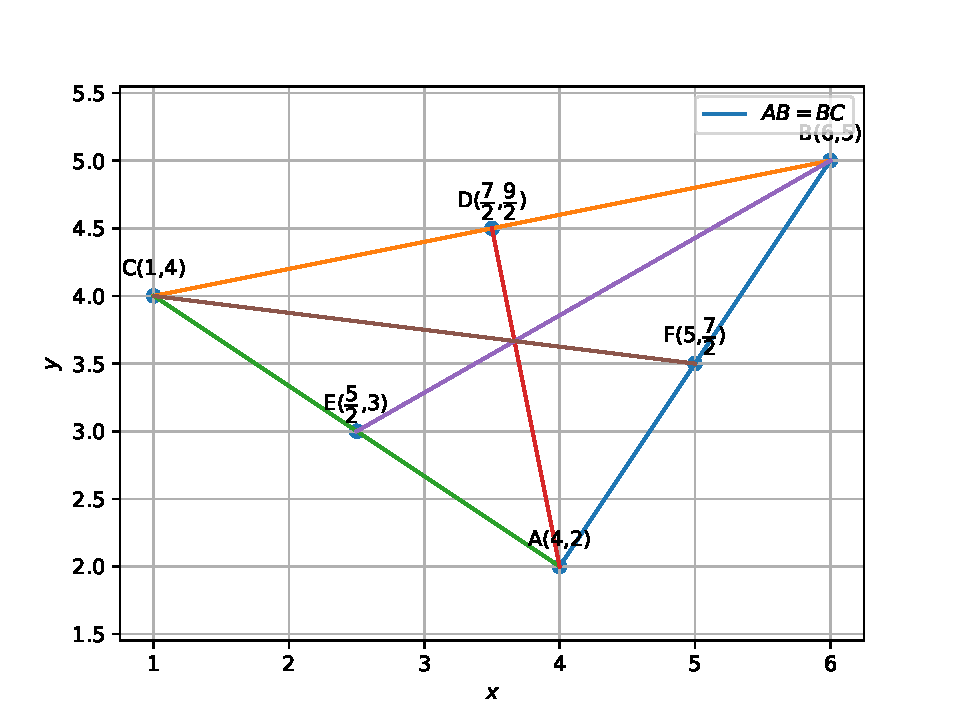
\includegraphics[width=\columnwidth]{chapters/10/7/4/7/figs/dj.pdf}
\caption{}
  \label{fig:chapters/10/7/4/7/Figure}
\end{figure}

\item Find the position vector of a point R which divides the line joining two points $P$ and $Q$ whose position vectors are $(2\vec{a}+\vec{b})$ and $(\vec{a}-3\vec{b})$
externally in the ratio 1 : 2. Also, show that $P$ is the mid point of the line segment $RQ$.\\
	\solution
		\iffalse
\documentclass[10pt]{article}
\usepackage{graphicx}
\usepackage[none]{hyphenat}
\usepackage{graphicx}
\usepackage{listings}
\usepackage[english]{babel}
\usepackage{siunitx}
\usepackage{graphicx}
\usepackage{caption} 
\usepackage{booktabs}
\usepackage{array}
\usepackage{amssymb} % for \because
\usepackage{amsmath}   % for having text in math mode
\usepackage{extarrows} % for Row operations arrows
\usepackage{listings}
\usepackage[utf8]{inputenc}
\lstset{
  frame=single,
  breaklines=true
}
\usepackage{hyperref}
  
%Following 2 lines were added to remove the blank page at the beginning
\usepackage{atbegshi}% http://ctan.org/pkg/atbegshi
\AtBeginDocument{\AtBeginShipoutNext{\AtBeginShipoutDiscard}}


%New macro definitions
\newcommand{\mydet}[1]{\ensuremath{\begin{vmatrix}#1\end{vmatrix}}}
\providecommand{\brak}[1]{\ensuremath{\left(#1\right)}}
\newcommand{\solution}{\noindent \textbf{Solution: }}
\newcommand{\myvec}[1]{\ensuremath{\begin{pmatrix}#1\end{pmatrix}}}
\providecommand{\norm}[1]{\left\lVert#1\right\rVert}
\providecommand{\abs}[1]{\left\vert#1\right\vert}
\let\vec\mathbf{}
\begin{document}

\begin{center}
\title{\textbf{VECTORS}}
\date{\vspace{-5ex}} %Not to print date automatically
\maketitle
\end{center}

\section*{12$^{th}$ Maths - EXERCISE-10.5}

Find the position vector of a point R which divides the line joining two points  P and Q whose position vectors are P = $\myvec{2\\ 1 \\}$ and Q = $\myvec{ 1\\-3\\ }$  externally in the ratio 1:2.Also show that P is the midpoint of the linesegment RQ.

\solution

\begin{align}
\vec{P} = \myvec{ 2\\1\\} 
 \label{eq1} \\
 \vec{Q} = \myvec{ 1\\-3\\}
\end{align}
\fi
When $\vec{R}$ divides line segment joining $\vec{P}$ and $\vec{Q}$ externally,
\begin{align}
\vec{R} &= \frac{\vec{Q} -2\vec{P}}{-1} 
= \myvec{3\\5}
\end{align}
Also,
\begin{align}
\frac{ (\vec{R} + \vec{Q})}{2}
=\myvec{2\\1} =\vec{P}
\end{align}
See Fig. 
\ref{fig:chapters/12/10/5/9/Figure1}.
\begin{figure}[!h]
	\begin{center}
		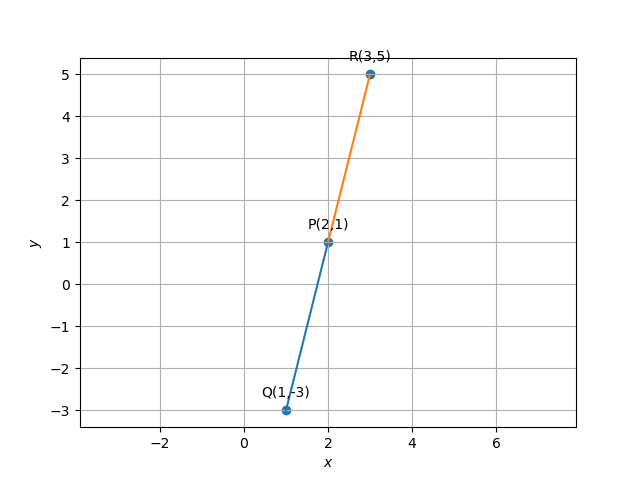
\includegraphics[width=\columnwidth]{chapters/12/10/5/9/figs/line.png}
	\end{center}
\caption{}
\label{fig:chapters/12/10/5/9/Figure1}
\end{figure}

\item The point which divides the line segment joining the points $\vec{P} (7, –6) $  and  $\vec{Q}(3, 4)$ in the 
ratio 1 : 2 internally lies in the
\begin{enumerate}
\item I quadrant
\item  II quadrant
\item  III quadrant
\item  IV quadrant
\end{enumerate}
\item If the point $\vec{P} (2, 1)$ lies on the line segment joining points $\vec{A} (4, 2)$  and $ \vec{B} (8, 4)$,
then
\begin{enumerate}
	\item $AP =\frac{1}{3}{AB}$ 
\item ${AP}={PE}$
\item ${PB}=\frac{1}{3}{AB}$
\item${AP}=\frac{1}{2}{AB}$
 \end{enumerate}
\item A line intersects the y-axis and x-axis at the points $\vec{P}$  and $\vec{Q}$, respectiveiy. lf $(2,5)$ is the mid-point of $\vec{PQ}$, then the coordinates of $\vec{P}$ and $ \vec{Q}$ are, respectively
\begin{enumerate}
	\item$(0,-5)$ and $(2,0)$
	\item$(0,-10)$ and $(-4,0)$
	\item$(0,4)$ and  $(-10,0)$
	\item$(0,-10)$ and $(4,0)$
\end{enumerate}
\item Point $\vec{P}(5,-3)$ is one of the two points of trisection of line segment joining the points $\vec{A}(7,-2)\text{ and }\vec{B}(1,-5)$
\item Points $\vec{A}(-6,10),\vec{B}(-4,6) \text{ and } \vec{C}(3,-8)$ are collinear such that $\vec{A}\vec{B}=  \frac{2}{9}\vec{A}\vec{C}$
\item In what ratio does the $x$-axis divide the line segment joining the points $(-4,-6)\text{ and }(-1,7)$? Find the coordinates of the point of division.
\item Find the ratio in which the point $\vec{P}\brak{\frac{3}{4},\frac{5}{12}}$ divides the line segment joining the points $\vec{A}\brak{\frac{1}{2},\frac{3}{2}}\text{ and } \vec{B}(2,-5)$.
\item If $\vec{P}(9a-2,-b)$ divides line segment joining $\vec{A}(3a+1,-3)\text{ and }\vec{B}(8a,5)$ in the ratio 3:1, find the values of $a$ and $b$.
\item The line segment joining the points $\vec{A}(3,2)\text{ and }\vec{B}(5,1)$ is divided at the point $\vec{P}$ in the ratio 1:2 which lies on $3x-18y+k=0$. Find the value of $k$.  
\item Find the coordinates of the point $\vec{R}$ on the line segment joining the points $\vec{P}(-1,3)\text{ and }\vec{Q}(2,5)$ such that $PR=\frac{3}{5}PQ$.
\item Find the ratio in which the line $2x+3y-5=0$ divides the line segment joining the points $(8,-9)$ and $(2,1)$. Also find the coordinates of the point of division.
\item If $\vec{a}$ and $\vec{b}$ are the postion vectors of $A$ and $B$, respectively, find the position vector of a point $C$ in $BA$ produced such that $BC=1.5BA$.
\item The position vector of the point which divides the join of points 2$\vec{a}$-3$\vec{b}$ $\text{and}$ $\vec{a}+\vec{b}$ in the ratio 3:1 is
	\begin{enumerate}
\item $\frac{3\vec{a}-2\vec{b}}{2}$
\item $\frac{7\vec{a}-8\vec{b}}{4}$
\item $\frac{\vec{3a}}{4}$
\item $\frac{\vec{5a}}{4}$
\end{enumerate}
\item Find the ratio in which the line segment joining $A(1,-5) \text{ and } B(-4,5)$ $\text{is divided by the x-axis}$. Also find the coordinates of the point of division.
\item Find the position vector of a point $\vec{R}$ which divides the line joining two points $\vec{P}$ and $\vec{Q}$ whose position vectors are $2\vec{a}+\vec{b}$ and $\vec{a}-3\vec{b}$ externally in the ratio $1:2$.
\item Find the coordinates of the point which divides the line segment joining the points which divides the line segment joining  the points $(-2,3,5)$ and $(1,-4,6)$ in the ratio 
\begin{enumerate}
\item $2:3$ internally,
\item $2:3$ externally
\end{enumerate}
\item Given that $P(3,2,-4), Q(5,4,-6)$ and $R(9,8,-10)$ are collinear. Find the ratio in which $Q$ divides $PR$.
\item Find the ratio in which the $yz$ plane divides the line segment formed by joining the points $(-2,4,7)$ and $(3,-5,8)$.
\item Find the coordinates of the points which trisect the line segment joining the points $P(4,2,-6)$ and $Q(10,-16,6)$.
\end{enumerate}

\subsection{CBSE}
\begin{enumerate}[label=\thesubsection.\arabic*,ref=\thesubsection.\theenumi]
\item The centre of a circle whose end points of a diameter are \brak{-6,3} and \brak{6,4} is
\hfill (10, 2020)
\item Find the ratio in which the $Y$ axis  divides the line segment joining the points \brak{6, -4} and \brak{-2, -7}. Also find the point of intersection.
\hfill (10, 2020)
    \item In what ratio does the $x$-axis divide the line segment joining the points $\vec{A}(3,6)$ and $\vec{B}(-12, -3)$?
    \hfill (10, 2023)
    \item A circle has its center at $(4,4)$. If one end of a diameter is $(4,0)$, then find the coordinates of the other end.
    \hfill (10, 2022)
	\item Find the coordinates of the point which divides the line segment joining the points $\vec{A}(7, -1)$ and $\vec{B}(-3, -4)$ in the ratio $2:3$. \hfill (10, 2021)
		\item The point which divides the line segment joining the points $(7, -6)$ and $(3, 4)$ in the ratio $1:2$ is
		\hfill (10, 2021)
		\item If $\left(\frac{a}{3}, 4\right)$ is the midpoint of the line segment joining the points $(-6, 5)$ and $(-2, 3)$, then the value of $a$ is
		\hfill (10, 2021)
		\item Find the ratio in which $\vec{P}(4, 5)$ divides the line segment joining $\vec{A}(2, 3)$ and $\vec{B}(7, 8)$. \hfill (10, 2021)
		\item Find the ratio in which the y-axis divides the line segment joining the points $\vec{A}(5, -6)$ and $\vec{B}(-1, -4)$. Also, find the coordinates of the point of intersection. \hfill (10, 2021)
		\item Find the ratio in which the line segment joining the points $\vec{A}(1, -5)$ and $\vec{B}(-4, 5)$ is divided by the x-axis. Also, find the coordinates of the point of division. \hfill (10, 2021)
\item The point $R$ divides the line segment $AB$, where $A(-4, 0)$ and $B(0, 6)$ such that $AR = \frac{3}{4} AB$. Find the coordinates of $R$. \hfill (10, 2019)
\item In what ratio does the point $P(-4, y)$ divide the line segment joining the points $A(-6, 10)$ and $B(3, -8)$? Hence, find the value of $y$. \hfill (10, 2019)
\item Find the ratio in which the $y$-axis divides the line segment joining the points $(-1, -4)$ and $(5, -6)$. Also find the coordinates of the point of intersection. \hfill (10, 2019)
\item Points $P$ and $Q$ trisect the line segment joining the points $A(-2, 0)$ and $B(0, 8)$ such that $P$ is nearer to $A$. Find the coordinates of points $P$ and $Q$. \hfill (10, 2019)
\item The midpoint of the line segment joining $A(2a, 4)$ and $B(-2, 3b)$ is $(1, 2a + 1)$. Find the values of $a$ and $b$. \hfill (10, 2019)
\item Find the coordinates of a point $A$ where $AB$ is a diameter of the circle with center $(3, -1)$ and the point $B$ is $(2, 6)$. \hfill (10, 2019)
\item The midpoint of the line segment joining $A(2a, 4)$ and $B(-2, 3b)$ is $(1, 2a + 1)$. Find the values of $a$ and $b$. \hfill (10, 2019)
\item Find the coordinates of a point $A$ where $AB$ is the diameter of a circle whose center is $(2, -3)$ and $B$ is the point $(1, 4)$. \hfill (10, 2019)
\item Find the ratio in which the segment joining the points $(1, 3)$ and $(4, 5)$ is divided by the $x$-axis. Also find the coordinates of this point on the $x$-axis. \hfill (10, 2019)
\item Find the coordinates of a point $A$ where $AB$ is a diameter of the circle with center $(-2, 2)$ and $B$ is the point $(3, 4)$. \hfill (10, 2019)

\end{enumerate}

\subsection{Rank}
\begin{enumerate}[label=\thesubsection.\arabic*,ref=\thesubsection.\theenumi]
\item 
 By using the concept of equation of a line, prove that the three points (3, 0), (– 2, – 2) and (8, 2) are collinear.
\label{chapters/11/10/2/20}
	\\
	\solution 
			From \eqref{eq:line-rank-2},
the collinearity matrix can be expressed as
 \begin{align}
			    \myvec{-5 & -2
			    \\
			    5 & 2 }  
			    \xleftrightarrow[]{R_2 \leftarrow {R_1 + R_2}}
			    \myvec{	    -5 & -2  
			    \\
			    0 & 0}  
\end{align}
which is a rank 1 matrix. The above process is known as row reduction, where we try to obtain zero rows in the matrix using arithmetic operations.  The number of nonzero rows in the row reduced matrix (also known as {\em echelon form})
is defined as the rank.
		\figref{fig:11/10/2/20}.
	\begin{figure}[H]
		\centering
 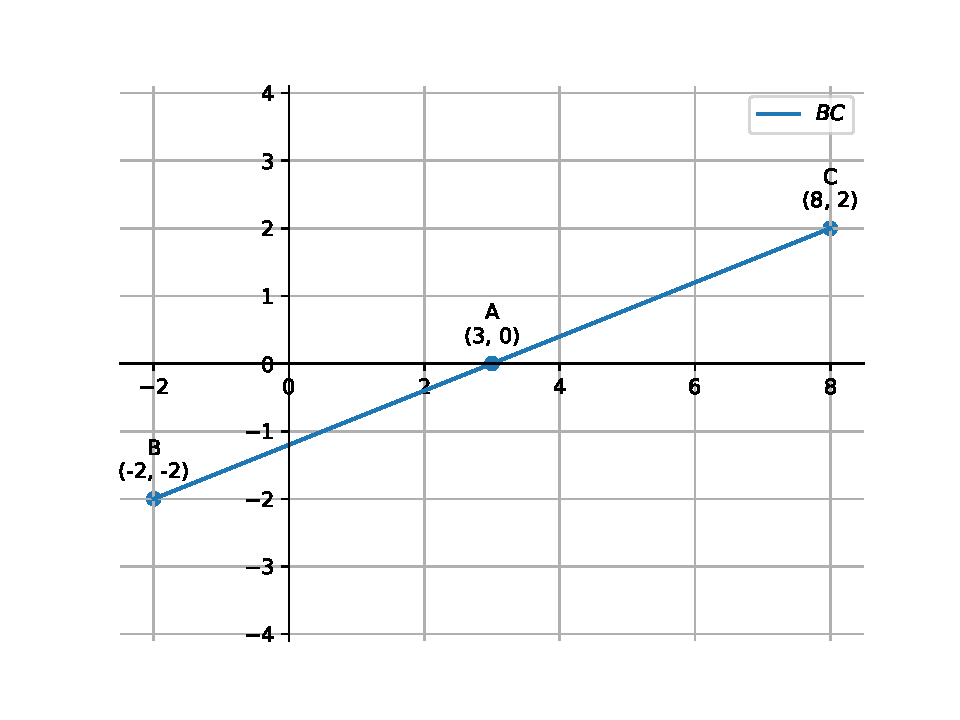
\includegraphics[width=0.75\columnwidth]{chapters/11/10/2/20/figs/fig.pdf}
		\caption{}
		\label{fig:11/10/2/20}
  	\end{figure}

\item Show that the points $\vec{A}(1,2,7), \vec{B}(2,6,3)$ and $\vec{C}(3,10,-1)$ are collinear.
	\\
		\solution The matrix
\begin{align}
	\myvec{\vec{B}-\vec{A}& \vec{C}-\vec{A}}^\top 
	= \myvec{1 & 4 & -4 \\ 2 & 8 & -8}
	\\
	\xleftrightarrow[]{R_2 = R_2 - 2R_1}
	 \myvec{1 & 4 & -4 \\ 0 & 0 & 0}
\end{align}
which has rank 1.  Using 
			\eqref{eq:mat-rank-t},
			 we conclude that the given points are collinear.
\item Determine if the points $(1,5),(2,3)$ and $(-2,-11)$ are collinear.
\item Show that the vectors $2\hat{i}-3\hat{j}+4\hat{k}$ and $-4\hat{i}+6\hat{j}-8\hat{k}$ are collinear.
\item Show that the points (2, 3, 4), (–1, –2, 1), (5, 8, 7) are collinear.
\item In each of the following, find the value of $k$, for which the points are collinear.
\begin{enumerate}
\item $(7, –2), (5, 1), (3, k)$
\item $(8, 1), (k, – 4), (2, –5)$
\end{enumerate}
		\label{10/7/3/2}
\item Find a relation between $x$ and $y$ if the points $(x, y), (1, 2)$  and  $(7, 0)$ are collinear.
\item If three points $(x, -1), (2, 1)$ and $(4, 5)$ are collinear, find the value of $x$.
\label{chapters/11/10/1/8}
\item If three points $(h, 0), (a, b)$ and $(0, k)$ lie on a line, 
show that 
\begin{align}
\frac{a}{h}+\frac{b}{k}=1
\end{align}
\label{chapters/11/10/1/13}
\item Show that the points $A (1, -2, -8), B (5, 0, -2)$ and $C (11, 3, 7)$ are collinear, and find the ratio in which $B$ divides $AC$.
\item lf the points $\vec{A}(1,2),\vec{0}(0,0)$ and $\vec{C}(a,b)$ are collinear,then find the relation between $a$ and $b$.
	\item Point $ (-4,2)$ lies on the line segment joining the points $ \vec{A}(-4,6)$  and  $\vec{B}(-4,-6)$.
 \item The points $(0,5),(0,-9)$ and $(3,6)$ are collinear.
\item Points $\vec{A}(3,1), \vec{B}(12,-2)$  and  $\vec {C}(0,2)$ cannot be the vertices of a triangle.
\item Find the value of $m$ if the points $(5,1),(-2,-3)$  and $(8,2m)$ are collinear.
\item Find the values of $k$ if the points $\vec{A}(k+1,2k),\vec{B}(3k,2k+3)$ and $\vec{C}(5k-1,5k)$ are collinear.
\item Using vectors, find the value of $k$ such that the points $(k,-10,3)$, $(1,-1,3)$  and  $(3,5,3)$ are collinear.
\item The points $\vec{A}(2,1)$, $\vec{B}(0,5)$, $\vec{C}(-1,2)$ are collinear.
\item The vectors $\lambda\hat{i}+\lambda\hat{j}+2\hat{k}$, $\hat{i}+\lambda\hat{j}-\hat{k}$ $\text{ and }$ $2\hat{i}-\hat{j}+\lambda\hat{k}$ are coplanar if
	\begin{enumerate}
\item	$\lambda=-2$
\item $\lambda=0$
\item $\lambda=1$
\item	$\lambda=-1$
\end{enumerate}
\item Show that the points $(-2,3,5), (1,2,3)$ and $(7,0,-1)$ are collinear.
\item A point $R$ with x-coordinate $4$ lies on the line segment joining the points $P(2,-3,4)$ and $Q(,0,10)$. Find the coordinates of the point $R$.
\item Show that points $A(a, b+c), B(b, c+a), C(c, a+b)$ are collinear.
\item Show that the points $A(2,-3,4), B(-1,2,1)$ and $C(0,\frac{1}{3},2)$ are collinear.
\end{enumerate}

\subsection{CBSE}
\begin{enumerate}[label=\thesubsection.\arabic*, ref=\thesubsection.\theenumi]
    \item The value of $m$ which makes the points $(0,0)$, $(2m, -4)$, and $(3,6)$ collinear, is \underline{\hspace{1cm}}.
    \hfill (10, 2022)
		\item If $\vec{A}(1, 2)$, $\vec{O}(0, 0)$, and $\vec{C}(a, 6)$ are collinear, then the value of $a$ is
		\hfill (10, 2021)
	\item Show that the points $A(-2\hat{i} + 3\hat{j} + 5\hat{k})$, $B(\hat{i} + 2\hat{j} + 3\hat{k})$, and $C(7\hat{i} - \hat{k})$ are collinear. \hfill (12, 2019)
	\item Using vectors, prove that the points $(2, -1, 3)$, $(3, -5, 1)$, and $(-1, 11, 9)$ are collinear. \hfill (12, 2019)
\item Find the value of $p$ for which the points $(-5, 1)$, $(1, p)$, and $(4, -2)$ are collinear. \hfill (10, 2019)
\item Find a relation between $x$ and $y$ if the points $A(x, y)$, $B(-4, 6)$, and $C(-2, 3)$ are collinear. \hfill (10, 2019)
\item For what value of $p$ are the points $(2, 1)$, $(p, -1)$, and $(-1, 3)$ collinear? \hfill (10, 2019)
\item Using vectors, prove that the points $\brak{2,-1,3},\brak{3,-5,1}$ and $\brak{-1,11,9}$ are collinear.

\hfill (12, 2018) 
\item If the points $\vec{A} = (k+1, 2k)$, $\vec{B} = (3k, 2k + 3)$, and $\vec{C} = (5k-1, 5k)$ are collinear, then find the value of $k$. \hfill (10, 2017)
\end{enumerate}

\subsection{Length}
\begin{enumerate}[label=\thesubsection.\arabic*,ref=\thesubsection.\theenumi]
\item Compute the magnitude of the following vectors:
\begin{align}
	\vec{a}&=\hat{i}+\hat{j}+\hat{k}
	\\
	\vec{b}&=2\hat{i}-7\hat{j}-3\hat{k}
	\\
	\vec{c}&=\frac{1}{\sqrt{3}}\hat{i}+\frac{1}{\sqrt{3}}\hat{j}-\frac{1}{3}\hat{k}
\end{align}
    \solution 
		Let 
\begin{align}
	\vec{a} = \myvec{1\\1\\1} , \vec{b} = \myvec{2\\ -7 \\ 3}, 
\vec{c} = \myvec{\dfrac{1}{\sqrt{3}}\\[2ex] \dfrac{1}{\sqrt{3}} \\[2ex] -\dfrac{1}{\sqrt{3}}} 
\label{eq:chapters/12/10/2/1/1}
\end{align}
Then
\begin{align}
	\norm{\vec{a}}&=\sqrt{\vec{a}^{\top}\vec{a}}=\sqrt{3}, 
	\label{eq:chapters/12/10/2/1/3}
	\\ \norm{\vec{b}}&=\sqrt{\vec{b}^{\top}\vec{b}}= \sqrt{62}, 
	\label{eq:chapters/12/10/2/1/4}
	\\ \norm{\vec{c}}&=\sqrt{\vec{c}^{\top}\vec{c}}	
=1
	\label{eq:chapters/12/10/2/1/5}
\end{align}




\item Find the value of $x$ for which $x(\hat{i}+\hat{j}+\hat{k})$ is a unit vector.\\
	\solution
		\begin{align} 
\because
\vec{x}=x\myvec{1\\1\\1},
\norm{\vec{x}}=1
\implies 
x\sqrt{3}=1
\\
	\text{or, }x=\frac{1}{\sqrt{3}}
\end{align}   

\item For given vectors, $\vec{a}=2\hat{i}-\hat{j}+2\hat{k}$ and $\vec{b}=-\hat{i}+\hat{j}-\hat{k}$ , find the unit vector in the
direction of the vector $\vec{a}+\vec{b}$.
        \label{prob:12/10/2/9}
\\
    \solution 
		\begin{align}
	\because \vec a + \vec b = \myvec{ 2\\-1\\2 } + \myvec{ -1\\1\\-1 },
= \myvec{ 1\\0\\1 },
\\
	\norm{\vec a + \vec b } = \sqrt{2}
	\\
	\implies \frac{\vec a + \vec b }{\norm{\vec a + \vec b }} = \frac{1}{\sqrt{2}}\myvec{ 1\\0\\1 }
\end{align}
which, from  \eqref{eq:unit-vec} is the desired the unit vector.
		





\item Find a vector in the direction of vector $5\hat{i}-\hat{j}+2\hat{k}$ which has magnitude 8 units.
        \label{prob:12/10/2/10const}
   \\ 
    \solution 
		Let the required vector be 
    \begin{align}
c\myvec{5\\-1\\2}.
    \end{align}
    From the given information, 
    \begin{align}
        \norm{c\myvec{5\\-1\\2\\}} =  8 \\
	    \implies \abs{c} = \frac{4\sqrt{30}}{15}
        \label{eq:12/10/2/10const}
    \end{align}


\item Find the unit vector in the direction of sum of vectors $\vec{a}$= $2\hat{i}-\hat{j}+\hat{k}$  and  $\vec{b}=2\hat{j}+\hat{k}$.
\item If $\vec{a}$=$\hat{i}+\hat{j}+2\hat{k}$  and  $\vec{b}$=$2\hat{i}+\hat{j}-2\hat{k}$, find the unit vector in the direction of
	\begin{enumerate}
		\item 6$\vec{a}$   
		\item 2$\vec{a}$-$\vec{b}$
	\end{enumerate}

\item Find a unit vector in the direction of $\overline{PQ} $, where $P$ and $Q$ have co-ordinates (5,0,8) and (3,3,2),respectively.
\item The vector in the direction of the vector $\hat{i}-2\hat{j}+2\hat{k}$ that has magnitude 9 is
	\begin{enumerate}
\item $\hat{i}-2\hat{j}+2\hat{k}$
\item $\hat{i}-2\hat{j}$
\item $3(\hat{i}-2\hat{j}+2\hat{k})$
\item $9(\hat{i}-2\hat{j}+2\hat{k})$
\end{enumerate}
\item Find the unit vector in the direction of the vector $\vec{a}=\hat{i}+\hat{j}+2\hat{k}$.
\item Find the unit vector in the direction of vector $\overrightarrow{PQ}$ , where $\vec{P}$ and $\vec{Q}$ are the points
(1, 2, 3) and (4, 5, 6), respectively.
\item Find a vector of magnitude 5 units, and parallel to the resultant of the vectors $\vec{a}=2\hat{i}+3\hat{j}-\hat{k}$ and $\vec{b}=\hat{i}-2\hat{j}+\hat{k}$.\\
\item If $\vec{a}=\hat{i}+\hat{j}+\hat{k}, \vec{b}=2\hat{i}-\hat{j}+3\hat{k}$ and $\vec{c}=\hat{i}-2\hat{j}+\hat{k}$, find a unit vector parallel to the vector $2\vec{a}-\vec{b}+3\vec{c}$.\\
	\solution
		\begin{align}
2\vec{a}-\vec{b}+3\vec{c}=\myvec{3\\-3\\2}
\implies
\frac{2\vec{a}-\vec{b}+3\vec{c}}{\norm{2\vec{a}-\vec{b}+3\vec{c}}}
=\frac{1}{\sqrt{22}}\myvec{3\\-3\\2}
\end{align}


	\item 
Find a vector of magnitude 5 units, and parallel to the resultant of the vectors $\vec{a} = 2\hat{i}+3\hat{j}-\hat{k}$ and $\vec{b} = \hat{i}-2\hat{j}+\hat{k}$.
\\
\solution
		\begin{align}
\because     \Vec{a}=\myvec{
        2\\3\\-1
    },\Vec{b}=\myvec{
        1\\-2\\1
    }\\
	\vec{a}+\vec{b}=\myvec{
        3\\1\\0
    }
    \implies
	\norm{\vec{a}+\vec{b}}=\sqrt{10}
\end{align}
From problem
        \ref{prob:12/10/2/9},
the unit vector in the direction of 
${\vec{a}+\vec{b}}$
is
\begin{align}
	\frac{{\vec{a}+\vec{b}}}{\norm{\vec{a}+\vec{b}}}
=\frac{1}{\sqrt{10}}\myvec{
        3\\1\\0
    }
\end{align}
The desired vector can then be expressed as
\begin{align}
\pm\frac{5}{\sqrt{10}}\myvec{
        3\\1\\0
    }
\end{align}


	\item If a line makes angles $90\degree,135\degree,45\degree$ with x,y and z-axis respectivly. Find its direction cosines.
		\\
		\solution
				From \eqref{eq:dir-vec-3d},
the direction vector is
\begin{align}
\vec{A}=\myvec{\cos 90\degree\\ \cos 135\degree\\ \cos 45\degree}=\myvec{0\\-\frac{1}{\sqrt{2}}\\ \frac{1}{\sqrt{2}}}
\end{align}

\item Find the direction cosines of the vector joining the points $\vec{A}$ (1, 2, –3) and
$\vec{B}$(–1, –2, 1), directed from $\vec{A}$ to $\vec{B}$.
	\\
    \solution 
		The unit vector  in the direction of AB is 
\begin{align}
	\frac{\vec{B}-\vec{A}}{\norm{\vec{B}-\vec{A}}}
	= \frac{1}{3}{\myvec{-1\\-2\\2}}
\end{align}
and the direction cosines are the elements of the above vector.

\item Show that the vector $\hat{i}+\hat{j}+\hat{k}$ is equally inclined to the axes OX, OY and OZ.
	\\
\solution
		Since all entries of the given vector 
\begin{align}
\myvec{1\\1\\1}
\end{align}
are equal, it is equally inclined to the axes.

\item If a line has the direction ratios –18, 12, –4, then what are its direction cosines?
		\\
		\solution
		Let
\begin{align}
	\vec{A} =\myvec{-18\\12\\-4}
\end{align}
Then the unit direction vector of the line is
\begin{align}
		\frac{\vec{A}}{\norm{\vec{A}}} =
\myvec{\frac{-9}{11}\\[2pt] \frac{6}{11}\\[2pt] \frac{-2}{11}}
\end{align}

	\item Find the direction cosines of the sides of a triangle whose vertices are $\myvec{3\\ 5\\-4 }$, $\myvec{ -1\\1 \\2 }$ and $\myvec{-5 \\-5 \\-2 }$.
		\\
		\solution
		Let the vertices be
\begin{align}
\vec{A} = \myvec{3\\5\\-4},
\vec{B} = \myvec{-1\\1\\2},
\vec{C} = \myvec{-5\\-5\\-2}
\end{align}
%
The direction vectors of the sides are,
\begin{align}
\vec{A} - \vec{B} = \myvec{4\\4\\-6} = \vec{m_1},
\vec{B} - \vec{C} = \myvec{4\\6\\4} = \vec{m_2}, 
\\
\vec{C} - \vec{A} = \myvec{-8\\-10\\2} =\vec{m_3},
\end{align}
%
The corresponding unit vectors are then obtained as
\begin{align}
 \myvec{ \frac{2}{\sqrt{17}} \\[1pt] \frac{2}{\sqrt{17}} \\[1pt] \frac{-3}{\sqrt{17}} },
 \myvec{ \frac{2}{\sqrt{17}} \\[1pt] \frac{3}{\sqrt{17}} \\[1pt] \frac{2}{\sqrt{17}} }, 
 \myvec{ \frac{-4}{\sqrt{42}} \\[1pt] \frac{-5}{\sqrt{42}} \\[1pt] \frac{1}{\sqrt{42}} } 
\end{align}

\item Find the direction cosines of the vector $\hat{i}+2\hat{j}+3\hat{k}$.
	\\
    \solution 
		The unit vector in the direction of the given vector is 
\begin{align}
	\vec{A} =\frac{1}{\sqrt{14}}\myvec{1\\2\\3}
\end{align}

    \item Find the direction cosines of a line which makes equal angles with the coordinate
    axes.
		\\
		\solution
		Let $\alpha$ be the angle made by the line with the axes.  The unit direction vector can be expressed as
    \begin{align}
	    \vec{x} &= \myvec{\cos\alpha\\\cos\alpha\\\cos\alpha} 
	\implies
	    \norm{\vec{x}}  = 1
	\\
	    \text{or, }\cos\alpha &= \frac{1}{\sqrt{3}}
    \end{align}
    Thus the unit direction vector  of the given line is 
    \begin{align}
	    \vec{x} = \frac{1}{\sqrt{3}} \myvec{1 \\ 1 \\ 1} 
\end{align}
    

\item If a unit vector $\overrightarrow{a}$ makes angles $\frac{\pi}{3}\text{ with }\hat{i}, \frac{\pi}{4}\text{ with }\hat{j}$ and an acute angle $\theta \text{ with }\hat{k},\text{ then find } \theta$ and hence, the components of $\overrightarrow{a}$.
	\\
		\solution
		From the given information,
		\begin{align}
			\vec{a}=\myvec{\cos\frac{\pi}{3}\\\cos\frac{\pi}{4}\\\cos\theta}
			= 
\myvec{\frac{1}{2}\\[1ex]\frac{1}{\sqrt{2}}\\[1ex]\cos\theta}
		\end{align}
\begin{align}
\because    \norm{\vec{a}}&=1,
\\
\frac{1}{4}+\frac{1}{2}+\cos^2\theta&=1
\\
    \implies\cos\theta &=\frac{1}{2}
\end{align}
$\because \theta$ is an acute angle.
    Hence 
\begin{align}
		\vec{a}=\myvec{\frac{1}{2}\\[1ex] \frac{1}{\sqrt{2}}\\[1ex] \frac{1}{2}}
\end{align}

\item Write down a unit vector in XY-plane, making an angle of 30$\degree$ with the positive direction of x-axis.\\
\item A vector $\vec{r}$ is inclined at equal angles to the three axis. If the magnitude of $\vec{r}$ is $2\sqrt{3}$ units, find $\vec{r}$.
\item The direction cosines of the vector $(2\hat{i}+2\hat{j}-\hat{k})$ are \noindent\rule{2cm}{0.4pt}.
\item A vector $\vec{r}$ has a magnitude 14 and direction ratios 2, 3, -6. Find the direction cosines and components of $\vec{r}$, given that $\vec{r}$ makes an acute angle with x-axis.
\end{enumerate}

\subsection{CBSE}
\begin{enumerate}[label=\thesubsection.\arabic*, ref=\thesubsection.\theenumi]
\item The distance between the points \brak{m, -n} and \brak{-m, n} is
\begin{enumerate}
\item \(\sqrt{m^{2} + n^{2}}\)
\item \(m + n\)
\item \(2\sqrt{m^{2} + n^{2}}\)
\item \(\sqrt{2m^{2} + 2n^{2}}\)
\end{enumerate}
\hfill (10, 2020)

\item The point on the $X$ axis which is equidistant from \brak{-4,0} and \brak{10,0} is
\begin{enumerate}
\item \brak{7,0}
\item \brak{5,0}
\item \brak{0,0}
\item \brak{3,0}
\end{enumerate}
\hfill (10, 2020)
%
\item \(AOBC\) is a rectangle whose three vertices are \brak{0, -3}, \brak{0, 0} and \brak{4, 0}. The length of its diagonal is
\hfill (10, 2020)
\item If $\mydet{\overrightarrow{a}}= 4$ and $-3 \leq \lambda \leq 2$, then $\mydet{\lambda \overrightarrow a}$ lies in
\begin{enumerate}
\item $\sbrak{0,12}$
\item $\sbrak{2,3}$
\item $\sbrak{8,12}$
\item $\sbrak{-12,8}$
\end{enumerate}
\hfill (12, 2020)
    \item The distance between the point $(0,2\sqrt{5})$ and $(-2\sqrt{5},0)$ is
    \hfill (10, 2023)
    \item If $\vec{Q} = (0,1)$ is equidistant from $CA = (5,-3)$ and $\vec{R} = (x,6)$, find the value of $x$.
    \hfill (10, 2023)
    \item The distance of the point $(-6,8)$ from the origin is
    \hfill (10, 2023)
    \item The distance between the points $(0,0)$ and $(a-b, a+b)$ is 
    \hfill (10, 2022)
	\item Find the distance between the points $\vec{A}\left(-\frac{7}{3}, 5\right)$ and $\vec{B}\left(\frac{2}{3}, 5\right)$. \hfill (10, 2021)
		\item The distance between the points $\vec{A}(0, 6)$ and $\vec{B}(0, -2)$ is
		\hfill (10, 2021)
		\item If the distance between the points $(k, -2)$ and $(3, -6)$ is $10$ units, find the positive value of $k$. \hfill (10, 2021)
		\item Find the length of the segment joining $\vec{A}(-6, 7)$ and $\vec{B}(-1, -5)$. Also, find the midpoint of $AB$. \hfill (10, 2021)
	
	\item A man goes $5$ meters due west and then $12$ meters due north. How far is he from the starting point? \hfill (10, 2021)
		\item If $\vec{P}(2, 2)$, $\vec{Q}(-4, -4)$, and $\vec{R}(5, -8)$ are the vertices of a triangle $\triangle PQR$, then find the length of the median through $\vec{R}$. \hfill (10, 2021)
	\item If $\vec{a}, \vec{b}, \vec{c}$ are position vectors of the points $A(2, 3, -4)$, $B(3, -4, -5)$, and $C(3, 2, -3)$ respectively, then $\abs{\vec{a}+\vec{b}+\vec{c}}$ is equal to
		\begin{enumerate}
			\item $\sqrt{113}$
			\item $\sqrt{185}$
			\item $\sqrt{203}$
			\item $\sqrt{209}$
		\end{enumerate}
	\hfill (12, 2021)
\item Find the distance between the points $(a, b)$ and $(-a, -b)$. \hfill (10, 2019)
\item Write the coordinates of a point $P$ on the $x$-axis which is equidistant from the points $A(-2, 0)$ and $B(6, 0)$. \hfill (10, 2019)
\item Find the value of $x$ if the distance between the points $A(0, 0)$ and $B(x, -4)$ is 5 units. \hfill (10, 2019)
\item Find the values of $x$ for which the distance between the points $A(x, 2)$ and $B(9, 8)$ is 10 units. \hfill (10, 2019)
\item Find the point on the $y$-axis which is equidistant from the points $(5, -2)$ and $(-3, 2)$. \hfill (10, 2019)
    \item Given vertices of a parallelogram $\vec{A}(-2,1)$, $\vec{B}(a,0)$, $\vec{C}(4,b)$, and $\vec{D}(1,2)$. Find the values of $a$ and $b$. Hence, find the lengths of its sides. \hfill (10, 2018)
    \item Find the value of $y$ for which the distance between the points $\vec{P}(2,-3)$ and $\vec{Q}(10,y)$ is $10$ units. \hfill (10, 2018)
    \item If the point $\vec{P}(0,2)$ is equidistant from the points $\vec{Q}(3,k)$ and $\vec{R}(k,5)$, find the value of $k$. \hfill (10, 2018)
    \item The x-coordinate of a point $\vec{P}$ is twice its y-coordinate. If $\vec{P}$ is equidistant from the points $\vec{Q}(2,-5)$ and $\vec{R}(-3,6)$, find the coordinates of $\vec{P}$. \hfill (10, 2018)
    \item If the point $P \myvec{x, y}$ is equidistant from the points $A \myvec{a+b, b-a}$ and $B \myvec{a-b, a+b}$, prove that $bx = ay$. \hfill (10, 2016)
\item The distance of the point $\brak{-3,4}$ from the $x$-axis is
\hfill (10, 2012)
\item Find the value of $k$, if the point $P\brak{2,4}$ is equidistant from the points $A\brak{5,k}$ and $B\brak{k,7}$. 
\hfill (10, 2012)
\item If a point $A\brak{0,2}$ is equidistant from the points $B\brak{3,p}$ and $C\brak{p,5}$, then find the value of $p$. 
\hfill (10, 2012)
\end{enumerate}

\subsection{Unit Vector}
\begin{enumerate}[label=\thesubsection.\arabic*, ref=\thesubsection.\theenumi]
\item Find the value of $x$ for which $x(\hat{i}+\hat{j}+\hat{k})$ is a unit vector.\\
	\solution
		\begin{align} 
\because
\vec{x}=x\myvec{1\\1\\1},
\norm{\vec{x}}=1
\implies 
x\sqrt{3}=1
\\
	\text{or, }x=\frac{1}{\sqrt{3}}
\end{align}   

\item For given vectors,  $\vec{a}=2\hat{i}-\hat{j}+2\hat{k}$ and $\vec{b}=-\hat{i}+\hat{j}-\hat{k}$ ,  find the unit vector in the
direction of the vector $\vec{a}+\vec{b}$.
        \label{prob:12/10/2/9}
\\
    \solution 
		\begin{align}
	\because \vec a + \vec b = \myvec{ 2\\-1\\2 } + \myvec{ -1\\1\\-1 },
= \myvec{ 1\\0\\1 },
\\
	\norm{\vec a + \vec b } = \sqrt{2}
	\\
	\implies \frac{\vec a + \vec b }{\norm{\vec a + \vec b }} = \frac{1}{\sqrt{2}}\myvec{ 1\\0\\1 }
\end{align}
which, from  \eqref{eq:unit-vec} is the desired the unit vector.
		





\item Find a vector in the direction of vector $5\hat{i}-\hat{j}+2\hat{k}$ which has magnitude 8 units.
        \label{prob:12/10/2/10const}
   \\ 
    \solution 
		Let the required vector be 
    \begin{align}
c\myvec{5\\-1\\2}.
    \end{align}
    From the given information, 
    \begin{align}
        \norm{c\myvec{5\\-1\\2\\}} =  8 \\
	    \implies \abs{c} = \frac{4\sqrt{30}}{15}
        \label{eq:12/10/2/10const}
    \end{align}


\item Find the unit vector in the direction of sum of vectors $\vec{a}$= $2\hat{i}-\hat{j}+\hat{k}$  and  $\vec{b}=2\hat{j}+\hat{k}$.
\item If $\vec{a}$=$\hat{i}+\hat{j}+2\hat{k}$  and  $\vec{b}$=$2\hat{i}+\hat{j}-2\hat{k}$,  find the unit vector in the direction of
	\begin{enumerate}
		\item 6$\vec{a}$   
		\item 2$\vec{a}$-$\vec{b}$
	\end{enumerate}

\item Find a unit vector in the direction of $\overline{PQ} $,  where $P$ and $Q$ have co-ordinates (5, 0, 8) and (3, 3, 2), respectively.
\item The vector in the direction of the vector $\hat{i}-2\hat{j}+2\hat{k}$ that has magnitude 9 is
	\begin{enumerate}
\item $\hat{i}-2\hat{j}+2\hat{k}$
\item $\hat{i}-2\hat{j}$
\item $3(\hat{i}-2\hat{j}+2\hat{k})$
\item $9(\hat{i}-2\hat{j}+2\hat{k})$
\end{enumerate}
\item Find the unit vector in the direction of the vector $\vec{a}=\hat{i}+\hat{j}+2\hat{k}$.
\item Find the unit vector in the direction of vector $\overrightarrow{PQ}$ ,  where $\vec{P}$ and $\vec{Q}$ are the points
(1,  2,  3) and (4,  5,  6),  respectively.
\item Find a vector of magnitude 5 units,  and parallel to the resultant of the vectors $\vec{a}=2\hat{i}+3\hat{j}-\hat{k}$ and $\vec{b}=\hat{i}-2\hat{j}+\hat{k}$.\\
\item If $\vec{a}=\hat{i}+\hat{j}+\hat{k},  \vec{b}=2\hat{i}-\hat{j}+3\hat{k}$ and $\vec{c}=\hat{i}-2\hat{j}+\hat{k}$,  find a unit vector parallel to the vector $2\vec{a}-\vec{b}+3\vec{c}$.\\
	\solution
		\begin{align}
2\vec{a}-\vec{b}+3\vec{c}=\myvec{3\\-3\\2}
\implies
\frac{2\vec{a}-\vec{b}+3\vec{c}}{\norm{2\vec{a}-\vec{b}+3\vec{c}}}
=\frac{1}{\sqrt{22}}\myvec{3\\-3\\2}
\end{align}


	\item 
Find a vector of magnitude 5 units,  and parallel to the resultant of the vectors $\vec{a} = 2\hat{i}+3\hat{j}-\hat{k}$ and $\vec{b} = \hat{i}-2\hat{j}+\hat{k}$.
\\
\solution
		\begin{align}
\because     \Vec{a}=\myvec{
        2\\3\\-1
    },\Vec{b}=\myvec{
        1\\-2\\1
    }\\
	\vec{a}+\vec{b}=\myvec{
        3\\1\\0
    }
    \implies
	\norm{\vec{a}+\vec{b}}=\sqrt{10}
\end{align}
From problem
        \ref{prob:12/10/2/9},
the unit vector in the direction of 
${\vec{a}+\vec{b}}$
is
\begin{align}
	\frac{{\vec{a}+\vec{b}}}{\norm{\vec{a}+\vec{b}}}
=\frac{1}{\sqrt{10}}\myvec{
        3\\1\\0
    }
\end{align}
The desired vector can then be expressed as
\begin{align}
\pm\frac{5}{\sqrt{10}}\myvec{
        3\\1\\0
    }
\end{align}


	\item If a line makes angles $90\degree, 135\degree, 45\degree$ with x, y and z-axis respectivly. Find its direction cosines.
		\\
		\solution
				From \eqref{eq:dir-vec-3d},
the direction vector is
\begin{align}
\vec{A}=\myvec{\cos 90\degree\\ \cos 135\degree\\ \cos 45\degree}=\myvec{0\\-\frac{1}{\sqrt{2}}\\ \frac{1}{\sqrt{2}}}
\end{align}

\item Find the direction cosines of the vector joining the points $\vec{A}$ (1,  2,  –3) and
$\vec{B}$(–1,  –2,  1),  directed from $\vec{A}$ to $\vec{B}$.
	\\
    \solution 
		The unit vector  in the direction of AB is 
\begin{align}
	\frac{\vec{B}-\vec{A}}{\norm{\vec{B}-\vec{A}}}
	= \frac{1}{3}{\myvec{-1\\-2\\2}}
\end{align}
and the direction cosines are the elements of the above vector.

\item Show that the vector $\hat{i}+\hat{j}+\hat{k}$ is equally inclined to the axes OX,  OY and OZ.
	\\
\solution
		Since all entries of the given vector 
\begin{align}
\myvec{1\\1\\1}
\end{align}
are equal, it is equally inclined to the axes.

\item If a line has the direction ratios –18,  12,  –4,  then what are its direction cosines?
		\\
		\solution
		Let
\begin{align}
	\vec{A} =\myvec{-18\\12\\-4}
\end{align}
Then the unit direction vector of the line is
\begin{align}
		\frac{\vec{A}}{\norm{\vec{A}}} =
\myvec{\frac{-9}{11}\\[2pt] \frac{6}{11}\\[2pt] \frac{-2}{11}}
\end{align}

	\item Find the direction cosines of the sides of a triangle whose vertices are $\myvec{3\\ 5\\-4 }$,  $\myvec{ -1\\1 \\2 }$ and $\myvec{-5 \\-5 \\-2 }$.
		\\
		\solution
		Let the vertices be
\begin{align}
\vec{A} = \myvec{3\\5\\-4},
\vec{B} = \myvec{-1\\1\\2},
\vec{C} = \myvec{-5\\-5\\-2}
\end{align}
%
The direction vectors of the sides are,
\begin{align}
\vec{A} - \vec{B} = \myvec{4\\4\\-6} = \vec{m_1},
\vec{B} - \vec{C} = \myvec{4\\6\\4} = \vec{m_2}, 
\\
\vec{C} - \vec{A} = \myvec{-8\\-10\\2} =\vec{m_3},
\end{align}
%
The corresponding unit vectors are then obtained as
\begin{align}
 \myvec{ \frac{2}{\sqrt{17}} \\[1pt] \frac{2}{\sqrt{17}} \\[1pt] \frac{-3}{\sqrt{17}} },
 \myvec{ \frac{2}{\sqrt{17}} \\[1pt] \frac{3}{\sqrt{17}} \\[1pt] \frac{2}{\sqrt{17}} }, 
 \myvec{ \frac{-4}{\sqrt{42}} \\[1pt] \frac{-5}{\sqrt{42}} \\[1pt] \frac{1}{\sqrt{42}} } 
\end{align}

\item Find the direction cosines of the vector $\hat{i}+2\hat{j}+3\hat{k}$.
	\\
    \solution 
		The unit vector in the direction of the given vector is 
\begin{align}
	\vec{A} =\frac{1}{\sqrt{14}}\myvec{1\\2\\3}
\end{align}

    \item Find the direction cosines of a line which makes equal angles with the coordinate
    axes.
		\\
		\solution
		Let $\alpha$ be the angle made by the line with the axes.  The unit direction vector can be expressed as
    \begin{align}
	    \vec{x} &= \myvec{\cos\alpha\\\cos\alpha\\\cos\alpha} 
	\implies
	    \norm{\vec{x}}  = 1
	\\
	    \text{or, }\cos\alpha &= \frac{1}{\sqrt{3}}
    \end{align}
    Thus the unit direction vector  of the given line is 
    \begin{align}
	    \vec{x} = \frac{1}{\sqrt{3}} \myvec{1 \\ 1 \\ 1} 
\end{align}
    

\item If a unit vector $\overrightarrow{a}$ makes angles $\frac{\pi}{3}\text{ with }\hat{i},  \frac{\pi}{4}\text{ with }\hat{j}$ and an acute angle $\theta \text{ with }\hat{k}, \text{ then find } \theta$ and hence,  the components of $\overrightarrow{a}$.
	\\
		\solution
		From the given information,
		\begin{align}
			\vec{a}=\myvec{\cos\frac{\pi}{3}\\\cos\frac{\pi}{4}\\\cos\theta}
			= 
\myvec{\frac{1}{2}\\[1ex]\frac{1}{\sqrt{2}}\\[1ex]\cos\theta}
		\end{align}
\begin{align}
\because    \norm{\vec{a}}&=1,
\\
\frac{1}{4}+\frac{1}{2}+\cos^2\theta&=1
\\
    \implies\cos\theta &=\frac{1}{2}
\end{align}
$\because \theta$ is an acute angle.
    Hence 
\begin{align}
		\vec{a}=\myvec{\frac{1}{2}\\[1ex] \frac{1}{\sqrt{2}}\\[1ex] \frac{1}{2}}
\end{align}

\item Write down a unit vector in XY-plane,  making an angle of 30$\degree$ with the positive direction of x-axis.\\
\item A vector $\vec{r}$ is inclined at equal angles to the three axis. If the magnitude of $\vec{r}$ is $2\sqrt{3}$ units,  find $\vec{r}$.
\item The direction cosines of the vector $(2\hat{i}+2\hat{j}-\hat{k})$ are \noindent\rule{2cm}{0.4pt}.
\item A vector $\vec{r}$ has a magnitude 14 and direction ratios 2,  3,  -6. Find the direction cosines and components of $\vec{r}$,  given that $\vec{r}$ makes an acute angle with x-axis.
\item Find the unit vector in the direction of vector $\overrightarrow{a} = 2\hat{i} +3\hat{j} +\hat{k}$.
\item Find the unit vector in the direction of the sum of the vectors, $\overrightarrow{a} = 2\hat{i} +2\hat{j} -5\hat{k}$ and $\overrightarrow{b} = 2\hat{i} +\hat{j} +3\hat{k}$.
\item Write the direction ratios of the vector $\overrightarrow{a} = \hat{i} +\hat{j} -\hat{k}$ and hence calculate its direction cosines.
\item Find the direction cosines of the unit vector perpendicular to the plane $\overrightarrow{r} \cdot(6 \hat{i}- 3 \hat{j}- 2 \hat{k})+ 1= 0$ passing through the origin.
\item If a line makes angle $90 \degree, 60 \degree$ and $30 \degree$ with the positive direction of x, y and z-axes respectively, find its direction cosines.
\item If a line has direction ratios $2, -1, -2$, determine its direction cosines.
\item Find the direction cosines of the line passing through the two points $(-2, 4, -5)$ and $(1, 2, 3)$.
\end{enumerate}

\subsection{CBSE}
\begin{enumerate}[label=\thesubsection.\arabic*,  ref=\thesubsection.\theenumi]
\item Find a vector $\overrightarrow{r}$ equally inclined to the three axes and whose magnitude is $3\sqrt{3}$ units.
\hfill (12,  2020)
    \item Unit vector along $PQ$,  where coordinates of $\vec{P}$ and $\vec{Q}$ respectively are (2, 1, -1) and (4, 4, -7),  is
    \hfill (12,  2023)
    \item If a line makes $60\degree$ and $45\degree$ angles with the positive directions of the $X$ axis and $Z$ axis respectively, then find the angle that it makes with the positive direction of the Y-axis. Hence, write the direction cosines of the line.
    \hfill (12, 2023)
    \item A vector of magnitude $9$ units in the direction of the vector $-2\hat{i} - \hat{j} + 2\hat{k}$ is \underline{\hspace{1cm}}.
	\item The scalar product of the vector $\overrightarrow{a} = \hat{i} + \hat{j} + \hat{k}$ with a unit vector along the sum of the vectors $\overrightarrow{b} = 2\hat{i} + 4\hat{j} - 5\hat{k}$ and $\overrightarrow{c} = \hat{\lambda} + 2\hat{j} + 3\hat{k}$ is equal to $1$. Find the value of $\lambda$ and hence find the unit vector along $\overrightarrow{b} + \overrightarrow{c}$. \hfill (12, 2019)
    \hfill (12, 2022)
	\item Find the direction cosines of a line which makes equal angles with the coordinate axes. \hfill (12, 2019)
	\item If a line has the direction ratios $-18, 12, -4$, then what are its direction cosines? 

		\hfill (12, 2019)
	\item Find the direction cosines of the line joining the points $\vec{P}(4, 3, -5)$ and $\vec{Q}(-2, 1, -8)$.

		\hfill (12, 2019)
\item If a line has direction ratios $-18, 12, -4$, what are its direction cosines? \hfill (12, 2018)
\item Find a unit vector perpendicular to both the vectors $\overrightarrow{a} = \hat{i} - 7\hat{j} + 7\hat{k}$ and $\overrightarrow{b} = 3\hat{i} - 2\hat{j} + 2\hat{k}$.

	\hfill (12, 2018)
\item Find the direction cosines of the line joining points $\vec{P}(4, 3, -5)$ and $\vec{Q}(-2, 1, 8)$.

	\hfill (12, 2018)
\item Find the direction cosines of the line joining points $\vec{P}$ $\brak{4,3,-5}$ and $\vec{Q}$ $\brak{-2,1,8}$.

\hfill (12, 2018)
\item The scalar product of the vector $\overrightarrow{a} = \hat{i} + \hat{j} + \hat{k}$ with a unit vector along the sum of the vector $\overrightarrow{b} = 2\hat{i} + 4\hat{j} - 5\hat{k}$ and $\overrightarrow{c} = \lambda \hat{i} + 2\hat{j} + 3\hat{k}$ is equal to $1$. Find the value of $\lambda$ and hence find the unit vector along $\overrightarrow{b} + \overrightarrow{c}$.
\hfill (12, 2018) 
\item If the sum of two unit vectors is a unit vector, prove that the magnitude of their difference is $\sqrt{3}$.
\hfill (12, 2018) 
\item If a line makes angles $ 90\degree,135\degree,45\degree$ with the x,y and z axes respectively,find its direction cosines.
\hfill (12, 2018) 
\item If $\overrightarrow{a} = 4\hat{i} - \hat{j} +\hat{k}$ and $\overrightarrow{b} = 2\hat{i} - 2\hat{j} + \hat{k}$, then find a unit vector parallel to the vector $\overrightarrow{a}+\overrightarrow{b}$. \hfill (12, 2016)
\item Write the direction ratios of the vector $3\vec{a}+2\vec{b}$ where $\vec{a} = \vec{i}+\vec{j}-2\vec{k}$ and $\vec{b} = 2\vec{i}-4\vec{j}+5\vec{k}$.

	\hfill (12, 2015)
\end{enumerate}

%
\newpage
\section{Vector Multiplication}
\subsection{Formulae}
\begin{enumerate}[label=\thesubsection.\arabic*.,ref=\thesubsection.\theenumi]
	\item The angle $\theta$ between $\vec{a}, \vec{b}$,
		is given by 
\begin{align}
	\label{eq:angle-inner}
		\cos\theta=\frac{{\vec{a}^{\top}}{\vec{b}}}{\norm{\vec{a}}\norm{\vec{b}}}
\end{align}
\item The equation of a line is given by 
\begin{align}
	\label{eq:param-form}
	\vec{x} = \vec{h} + \kappa \vec{m}
\end{align}
\item 
	For
\begin{align}
	\vec{m}^{\top}\vec{n} = 0,
\end{align}
	\eqref{eq:param-form} can be expressed as
\begin{align}
	\vec{n}^{\top}\vec{x} &= \vec{n}^{\top}\vec{h} + \kappa \vec{n}^{\top}\vec{m}
	\\
	\label{eq:normal-form}
\implies	\vec{n}^{\top}\vec{x} = c
\end{align}
for 
\begin{align}
c = 	\vec{n}^{\top}\vec{h}. 
\end{align}
$\vec{n}$ is defined to be the
{\em normal vector}
		of the line.  
	\item Mathematically, 
the projection of $\vec{A}$ on $\vec{B}$ is defined as
		\begin{align}
	\vec{C} = k \vec{B},\, \text{such that}
	\brak{\vec{A}-\vec{C}}^{\top}\vec{C} = 0
\end{align}
yielding
\begin{align}
	\brak{\vec{A}-k\vec{B}}^{\top}\vec{B} = 0
	\\
	\text{or, } k = 
	\frac{\vec{A}^{\top}\vec{B}}{\norm{\vec{B}}^2}
	\implies 
	\vec{C} = 
	\frac{\vec{A}^{\top}\vec{B}}{\norm{\vec{B}}^2}
 \vec{B}
	\label{eq:12/10/3/4/proj}
\end{align}
\item If $\vec{A}, \vec{B}$ are unit vectors, 
\begin{multline}
	\brak{\vec{A}-\vec{B}}^{\top} 
	\brak{\vec{A}+\vec{B}} 
	\\
\norm{\vec{A}}^2 - \norm{\vec{B}}^2
	= 0
	\label{eq:12/10/3/11/unit}
\end{multline}
  \item If 
\begin{align}
	\vec{A}^{\top}\vec{A} =\vec{I},
\label{eq:12/10/3/5/inner}
\end{align}
		then $	\vec{A}$ is an {\em orthogonal} matrix.
\item Let 
\begin{align}
  \vec{A} &= \myvec{a_1\\a_2 \\ a_3} \equiv a_1\overrightarrow{i}+a_2\overrightarrow{j}+a_3\overrightarrow{j}, 
  \\
  \vec{B} &= \myvec{b_1\\b_2 \\ b_3}, 
\end{align}
and 
\begin{align}
  \label{eq:cross3d-submat}
\begin{split}
  \vec{A}_{ij} &= \myvec{a_i\\a_j}, 
  \\
  \vec{B}_{ij} &= \myvec{b_i\\b_j}. 
\end{split}
\end{align}

\item The {\em cross product} or {\em vector product} of $\vec{A}, \vec{B}$ is defined as
\begin{align}
  \label{eq:cross3d}
	\vec{A} \times \vec{B} 
	 = \myvec{ \mydet{\vec{A}_{23} & \vec{B}_{23}} \\[1ex] \mydet{\vec{A}_{31} & \vec{B}_{31}} \\[1ex] \mydet{\vec{A}_{12}  & \vec{B}_{12}}}
\end{align}
\item Verify that
\begin{align}
  \label{eq:cross3d-commute}
  \vec{A} \times \vec{B} = -  \vec{B} \times \vec{A} 
  \\
  \label{eq:cross3d-same}
  \vec{A} \times \vec{A} = \vec{0}
\end{align}
\item If 
		\label{prop:lin-dep-cross}
\begin{align}
  \vec{A} \times \vec{B} = \vec{0},
\end{align}
  $\vec{A}$ and $ \vec{B} $ are linearly independent.
  \item 
\begin{align}
	\label{eq:cross-sin}
	\norm{ \vec{A} \times \vec{B} }
	=
	\norm{\vec{A}} \times 	\norm{\vec{B}} \sin \theta
\end{align}
where $\theta$ is the angle between the vectors.
\item 
\begin{align}
	ar\brak{ABCD} = 
         \frac{1}{2}\brak{\brak{\vec{C}-\vec{A}}\times\brak{\vec{D}-\vec{B}}} \\
        \label{eq:11/10/1/1area-diag} 
\end{align}
	\item 
The affine transformation is given by 
\begin{align}
	\label{eq:conic_affine}
	\vec{x} = \vec{P}\vec{y}+\vec{c}
\end{align}
where $\vec{c}$ is the translation vector.
\item The matrix
\begin{align}
\vec{P} =
\myvec{
\cos\theta & -\sin\theta \\
\sin\theta & \cos\theta 
}
\end{align}
is defined to be the rotation matrix. 
\item 
\begin{align}
	\vec{P}^{\top} \vec{P} = \vec{I}
\end{align}
		$\vec{P}$ is known as as {\em orthogonal} matrix.
\item Given vertices $\vec{A}, \vec{C}$ of a square, the other two vertices are given by
\begin{align}
\begin{split}
	\vec{B} = \norm{\vec{C}-\vec{A}}\cos \frac{\pi}{4}\vec{P}\vec{e}_1+\vec{A}
	\\
	\vec{D} = \norm{\vec{C}-\vec{A}}\cos \frac{\pi}{4}\vec{P}\vec{e}_2+\vec{A}
\end{split}
	\label{eq:affine-square-bd}
\end{align}
%-c}}{\norm{\vec{n}}}\vec{n}
	\\
		\solution Shifting $\vec{A}$ to the origin and rotating the square clockwise by an angle $\phi$ made by $CA$ with the $x$-axis,
	from \eqref{eq:conic_affine},
\begin{align}
\vec{A} = \vec{P}\vec{0}+\vec{c}
\\
\implies 
\vec{c} = \vec{A}
\\
	\theta =  \phi -\frac{\pi}{4} 
\end{align}
and we obtain a square with the other vertices as
\begin{align}
\begin{split}
	\vec{B}_1 = \norm{\vec{C}-\vec{A}}\cos \frac{\pi}{4}\vec{e}_1
	\\
	\vec{D}_1 = \norm{\vec{C}-\vec{A}}\cos \frac{\pi}{4}\vec{e}_2
\end{split}
	\label{eq:affine-bd}
\end{align}
	From \eqref{eq:conic_affine}
	and 
	\eqref{eq:affine-bd},
	we obtain \eqref{eq:affine-square-bd}.
\end{enumerate}

\subsection{Scalar Product}
\begin{enumerate}[label=\thesubsection.\arabic*,ref=\thesubsection.\theenumi]
\item Find the angle between two vectors $\overrightarrow{a}$ and $\overrightarrow {b} $ with magnitudes $\sqrt{3}$ and 2 respectively having $\overrightarrow {a}\cdot\overrightarrow {b}=\sqrt{6}$.
		\label{prob:12/10/3/1/inner}
	\\
	\solution
		From the given information,
\begin{align}
\norm{\vec{a}}=\sqrt{3},
\norm{\vec{b}}= 2,
{\vec{a}^{\top}}{\vec{b}}=\sqrt{6}  
\\
\implies \cos\theta=\frac{{\vec{a}^{\top}}{\vec{b}}}{\norm{\vec{a}}\norm{\vec{b}}}
=\frac{1}{\sqrt{2}}\\
	\text{or, }\theta={45}\degree
\end{align}

\item Find the angle between the the vectors $\hat{i}-2\hat{j}+3\hat{k}$ and $3\hat{i}-2\hat{j}+\hat{k}$.
	\\
	\solution
		Let 
\begin{align}
	\vec{a} = \myvec{1\\-2\\3} , \vec{b} = \myvec{3\\ -2 \\ 1},
\end{align}
		From problem \ref{prob:12/10/3/1/inner},
\begin{align}
\cos\theta=\frac{\vec{a}^{\top}\vec{b}}{\norm{\vec{a}}\norm{\vec{b}}}
	= \frac{10}{\sqrt{14}\times \sqrt{14}}= \frac{5}{7}
\end{align}

\item Evaluate the product $(3\overrightarrow {a}-5\overrightarrow {b})\cdot (2\overrightarrow {a}+7\overrightarrow {b})$.
	\\
	\solution
		\begin{multline}
    \brak{3\vec{a}-5\vec{b}}^{\top}\brak{2\vec{a}+7\vec{b}}= 3\vec{a}^{\top}\brak{2\vec{a}+7\vec{b}} - 5\vec{b}^{\top}\brak{2\vec{a}+7\vec{b}}
    \\
     =6\norm{\vec{a}}^2-35\norm{\vec{b}}^2+11\vec{a}^{\top}\vec{b}
\end{multline}

\item If the vertices $A,B,C$ of a triangle $ABC$ are (1,2,3), (-1,0,0), (0,1,2), respectively, then find  $\angle{ABC}$.
	\\
	\solution
		From the given information, 
\begin{align}
\vec{A} - \vec{B} &= \myvec{2\\2\\3},
\vec{C} - \vec{B} = \myvec{1\\1\\2}\\
	\implies \angle{ABC} &= \cos^{-1}{\frac{\brak{\vec{A} -\vec{B}}^{\top}\brak{\vec{C}-\vec{B}}}{\norm{\vec{A} -\vec{B}}  \norm{\vec{C}-\vec{B}}}}\\
&= \cos^{-1}{\frac{10}{\sqrt{102}}}\\
\end{align}




	\item The slope of a line is double of the slope of another line. If tangent of the angle between them is 1/3, find the slopes of the lines.
\label{chapters/11/10/1/11}
\\
\solution 
The direction vectors of the lines can be expressed as
\begin{align}
\vec{m}_1=\myvec{1\\m},
\vec{m}_2=\myvec{1\\2m}
\end{align}
If the angle between the lines be $\theta$,
\begin{align}
\tan \theta = \frac{1}{3}
\implies \cos \theta=\frac{3}{\sqrt{10}}
\end{align}
Thus,
\begin{align}
	\frac{3}{\sqrt{10}} = \frac{\vec{m}_1^\top \vec{m}_2}{\norm{\vec{m}_1}\norm{\vec{m}_2}}
	\\
	= \frac{2m^2 +1}{\sqrt{m^2 + 1}\sqrt{4m^2 + 1}}
	\\
	\implies \frac{9}{10}=\frac{4m^4 + 4m^2 +1}{4m^4 + 5m^2 +1}
\\
	\text{or, } 4m^4 - 5m^2 +1 = 0
\end{align}
yielding
\begin{align}
m=\pm \frac{1}{2}, 
\pm 1
\end{align}

\item    Find angle between the lines, $\sqrt{3}x+y=1$ and $x+\sqrt{3}y$=1.
\label{chapters/11/10/3/9}
\\
   \solution 
	From \eqref{eq:normal-form}, 
 the normal vectors of the given lines can be expressed as
   \begin{align}
	   \vec{n}_1=\myvec{\sqrt{3}\\1},\,
	   \vec{n}_2=\myvec{1\\\sqrt{3}}
   \end{align}
The angle between the lines can then be 
obtained as
\begin{align}
	\cos\theta=\frac{\vec{n}_1^\top\vec{n}_2}{\norm{\vec{n}_1}\norm{\vec{n}_2}}
	=\frac{\sqrt{3}}{2} 
	\\
	\text{or, }
\theta=30\degree
\end{align}

\item Find the angle between the vectors $2\hat{i}-\hat{j}+\hat{k}$ and $3\hat{i}+4\hat{j}-\hat{k}$.
\item The angles between two vectors $\vec{a}, \vec{b}$ with magnitude $\sqrt{3}, 4$ respectively, and $\vec{a} \cdot \vec{b}= 2\sqrt{3}$ is
	\begin{enumerate}
\item $\frac{\pi}{6}$
\item $\frac{\pi}{3}$
\item $\frac{\pi}{2}$ 
\item $\frac{5\pi}{2}$
\end{enumerate}
\item Find the angle between the lines 
\begin{align}
	\overrightarrow{r}&=3\hat{i}-2\hat{j}+6\hat{k}+\lambda(2\hat{i}+\hat{j}+2\hat{k})
	\text{ and}
	\\
	\overrightarrow{r}&=(2\hat{j}-5\hat{k})+\mu(6\hat{i}+3\hat{j}+2\hat{k})
\end{align}
%
\solution  The given lines can be expressed  in the form 
of 
	\eqref{eq:param-form}
	as
\begin{align}
	\vec{x} = \myvec{3 \\ -2 \\ 6} + \kappa_1 \myvec{2 \\ 1 \\ 2}
	\\
	\vec{x} = \myvec{0 \\ 2 \\ -5 } + \kappa_2 \myvec{6 \\ 3 \\ 2}
\end{align}
From the above, it is obvious that the direction vectors of the two lines are
\begin{align}
\vec{m}_1 =\myvec{2 \\ 1 \\ 2},\
	\vec{m}_2=\myvec{6 \\ 3 \\ 2}
\end{align}
	From \eqref{eq:angle-inner}, the angle between the two lines is  obtained as
\begin{align}
	\cos \theta = \frac{19}{21}
\end{align}
\item The vectors $\vec{a}=3\hat{i}-2\hat{j}+2\hat{k}$ $\text{ and }$ $\vec{b}=\hat{i}-2\hat{k}$ are the adjancent sides of a parallelogram. The acute angle between its diagonals is \rule{1cm}{0.15mm}.
\item The sine of the angle between the straight line 
\begin{align}
	\frac{x-2}{3}=\frac{y-3}{4}=\frac{z-4}{5} 
\end{align}
and the plane  
\begin{align}
2x-2y+z=5
\end{align}
is
\begin{enumerate}
	\item $\frac{10}{6\sqrt{5}}$ 
	\item $\frac{4}{5\sqrt{2}}$
	\item $\frac{2\sqrt{3}}{5}$
	\item $\frac{\sqrt{2}}{10}$
\end{enumerate}
\solution The given line can be expressed in the form 
	\eqref{eq:param-form}
	as
\begin{align}
	\vec{x} = \myvec{2 \\ 3 \\ 4} + \kappa_1 \myvec{3 \\ 4 \\ 5}
\end{align}
Hence the direction vector of this line is 
\begin{align}
\myvec{3 \\ 4 \\ 5}
\end{align}
	From \eqref{eq:normal-form}, the normal vector of the given plane is 
\begin{align}
\myvec{2 \\ -2 \\ 1}
\end{align}
Thus, the cosine of the angle between the two is 
obtained from \eqref{eq:angle-inner} as
\begin{align}
	\frac{\sqrt{2}}{10},
\end{align}
which is sine of the angle between the plane and the line.
\item The plane $2x-3y+6z-11=0$ makes an angle $\sin^{-1}(\alpha)$ with x-axis. The value of $\alpha$ is equal to 
\begin{enumerate}
	\item  $\frac{\sqrt{3}}{2}$
	\item  $\frac{\sqrt{2}}{3}$
	\item  $\frac{2}{7}$
	\item  $\frac{3}{7}$
\end{enumerate}
\item Find the angle between the vectors $2\hat{i}-\hat{j}+\hat{k}$ $\text{and}$ $3\hat{i}+4\hat{j}-\hat{k}$.
\item The angles between two vectors $\vec{a}$ $\text{and}$ $\vec{b}$ with magnitude $\sqrt{3}$ $\text{ and }$ 4, respectively, and $\vec{a}$, $\vec{b}$= $2\sqrt{3}$ is
	\begin{enumerate}
\item $\frac{\pi}{6}$
\item $\frac{\pi}{3}$
\item $\frac{\pi}{2}$ 
\item $\frac{5\pi}{2}$
\end{enumerate}

\item The angle between the line 
\begin{align}
	\overrightarrow{r}=(5\hat{i}-\hat{j}-4\hat{k})+\lambda(2\hat{i}-\hat{j}+\hat{k})
\end{align}
	and the plane 
\begin{align}
	\overrightarrow{r} \cdot (3\hat{i}-4\hat{j}-\hat{k})+5=0
\end{align}
	is $\sin^{-1}\brak{\frac{5}{2\sqrt{91}}}$.
\item The angle between the planes 
\begin{align}
	\overrightarrow{r} \cdot (2\hat{i}-3\hat{j}+\hat{k})&=1 
	\text{ and }
	\\
	\overrightarrow{r} \cdot (\hat{i}-\hat{j})&=4  
\end{align}
is
	$\cos^{-1} \brak{\frac{-5}{\sqrt{58}}}$.
\item Find the angle between the lines 
\begin{align}
	y&=(2-\sqrt{3})(x+5)\text{ and }
	\\
	y&=(2+\sqrt{3})(x-7).
\end{align}
\item The unit vector normal to the plane $x+2y+3z-6=0$ is $\frac{1}{\sqrt{14}}\hat{i} + \frac{2}{\sqrt{14}}\hat{j} + \frac{3}{\sqrt{14}}\hat{k}$.
\item The scalar product of the vector $\hat{i}+\hat{j}+\hat{k}$ with a unit vector along the sum of vectors $2\hat{i}+4\hat{j}-5\hat{k}$ and $\lambda\hat{i}+2\hat{j}+3\hat{k}$ is equal to one. Find the value of $\lambda$.
\end{enumerate}

\subsection{CBSE}
\begin{enumerate}[label=\thesubsection.\arabic*, ref=\thesubsection.\theenumi]
\item The angle between the vectors $\hat{i} - \hat{j}$ and $\hat{j} - \hat{k}$ is
\hfill (12, 2020)
\item Find the angle between unit vectors $\overrightarrow{a}$ and $\overrightarrow{b}$ so that $\sqrt{3}\overrightarrow{a}$ - $\overrightarrow{b}$ is also a unit vector.
\hfill (12, 2020)
    \item If $\overrightarrow{a}, \overrightarrow{b}, \overrightarrow{c}$ are three non-zero unequal vectors such that $\overrightarrow{a} \cdot \overrightarrow{b} = \overrightarrow{a} \cdot \overrightarrow{c}$, then find the angle between $\overrightarrow{a}$ and $\overrightarrow{b} - \overrightarrow{c}$.
    \hfill (12, 2023)
    \item $\overrightarrow{a}$ and $\overrightarrow{b}$ are two unit vectors such that
    \begin{align}
        \left| 2\overrightarrow{a} + 3\overrightarrow{b} \right| = \left| 3\overrightarrow{a} - 2\overrightarrow{b} \right|.
    \end{align}
  Find the angle between $\overrightarrow{a}$ and $\overrightarrow{b}$.
    \hfill (12, 2023)
	\item Find the angle between the line $\overrightarrow{r} = \hat{i} - \hat{j} + \hat{k} + \lambda (3\hat{i} - \hat{j} + 2\hat{k})$ and the plane $\overrightarrow{r} \cdot (\hat{i} + \hat{j} + \hat{k}) = 3$. \hfill (12, 2019)
\item Find the magnitude of each of the vectors $\overrightarrow{\vec{a}}$ and $\overrightarrow{\vec{b}}$, having the same magnitude such that the angle between them is $60\degree$ and their scalar product is $\frac{9}{2}$. \hfill (12, 2018)
\item Find the acute angle between the planes $\vec{r}$($ \hat{i}-\hat{2j}-\hat{2k})=1$ and $\vec{r}$($ \hat{3i}-\hat{6j}+\hat{2k})=0$
\hfill (12, 2018)
\item If $\hat{i}+\hat{j}+{k} ,  2\hat{i}+5\hat{j} ,  3\hat{i}+2\hat{j}-3{k} ,  \hat{i}-6\hat{j}-{k}$ respectively are the position vectors of points A, B, C and D, then find the angle between the straight lines AB and CD. Find whether $\overrightarrow{AB}$ and $\overrightarrow{CD}$ are collinear or not. 
\hfill (12, 2018) 
\item If vectors $\overrightarrow{a}$ and $\overrightarrow{b}$ are such that
      $\abs{\overrightarrow{a}} = \frac{1}{2}$, $\abs{\overrightarrow{b}} = \frac{4}{\sqrt{3}}$
      and $\abs{\overrightarrow{a} \times \overrightarrow{b}} = \frac{1}{\sqrt{3}}$, then find
      $\abs{\overrightarrow{a}.\overrightarrow{b} }$. \hfill (12, 2016)
\item If $\overrightarrow{a}$ and $\overrightarrow{b}$ are unit vectors, then what is the angle between
      $\overrightarrow{a}$ and $\overrightarrow{b}$ for $\overrightarrow{a} - \sqrt{2}\overrightarrow{b}$ to be a unit vector? \hfill (12, 2016)


\end{enumerate}

\subsection{Orthogonality}
\begin{enumerate}[label=\thesubsection.\arabic*,ref=\thesubsection.\theenumi]
\item Name the type of quadrilateral formed, if any, by the following points,and give reasons for your answer
\begin{enumerate}
\item $A(-1,-2), B(1,0), (C-1,2), D(-3,0)$
\item $A(-3,5), B(-3,1), C(0,3), D(-1,-4)$
\item $A(4,5), B(7,6), C(4,3), D(1,2)$
\end{enumerate}
\solution
			See \tabref{tab:10/7/1/6/inner},
	\figref{fig:10/7/1/6/Fig1}, \figref{fig:10/7/1/6/Fig2}.
	and 
	\figref{fig:10/7/1/6/Fig3}. 
In b), forming the collinearity matrix
\begin{align}
\myvec{\vec{B}-\vec{A} & \vec{C}-\vec{B}} 
=
		\myvec{6&-3\\-4&2} \xleftrightarrow{R_{2}\rightarrow R_{2}+\frac{2}{3}R_{1}}= \myvec{6&-3\\0&0}
\end{align}
which is a rank 1 matrix.  Hence, $\vec{A}, \vec{B}, \vec{C}$  are collinear.
\begin{figure}[H]
	\begin{center} 
	    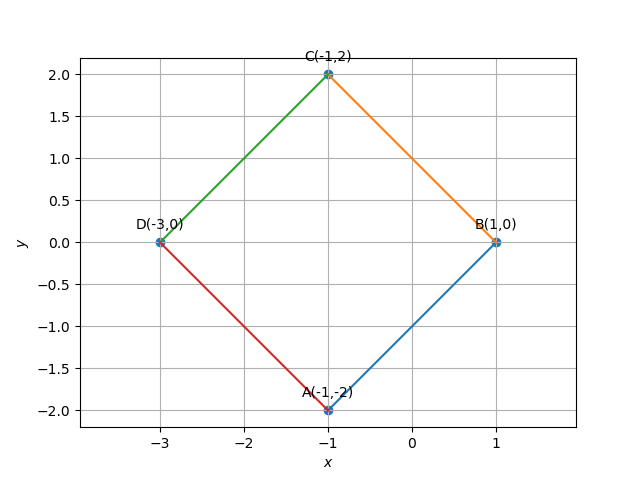
\includegraphics[width=0.75\columnwidth]{chapters/10/7/1/6/figs/quad1}
	\end{center}
\caption{}
\label{fig:10/7/1/6/Fig1}
\end{figure}
%
\begin{figure}[H]
	\begin{center} 
	    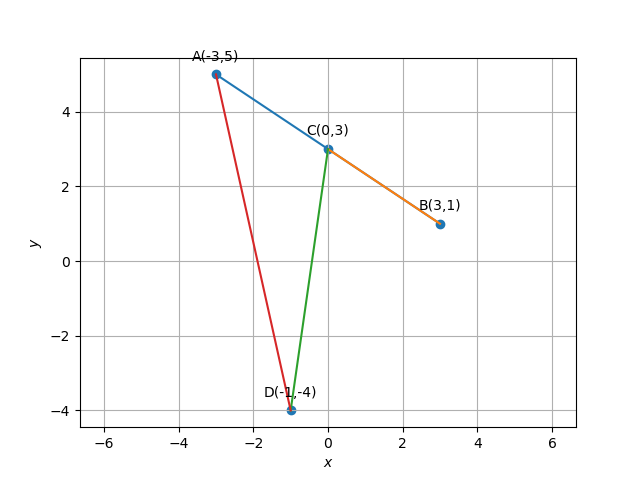
\includegraphics[width=0.75\columnwidth]{chapters/10/7/1/6/figs/quad2}
	\end{center}
\caption{}
\label{fig:10/7/1/6/Fig2}
\end{figure}
%	
\begin{figure}[H]
	\begin{center} 
	    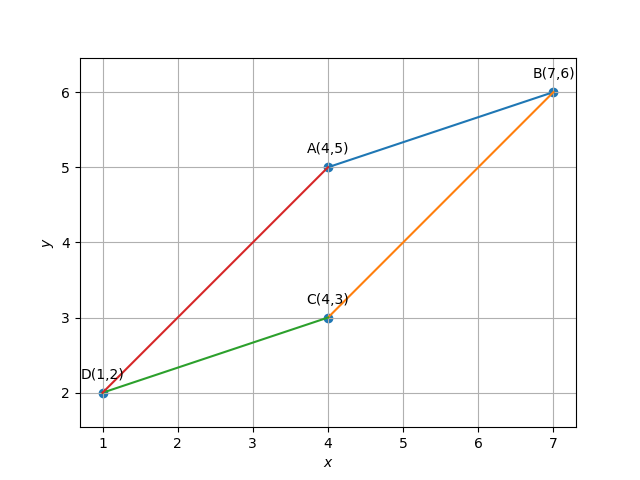
\includegraphics[width=0.75\columnwidth]{chapters/10/7/1/6/figs/quad3}
	\end{center}
\caption{}
\label{fig:10/7/1/6/Fig3}
\end{figure}
%
\begin{table}[H]
    \centering
%    \begin{tabular}{|c|c|c|c|c|}
	    \begin{tabularx}{\columnwidth}{|c|X|X|X|c|}
        \hline
		    &{\scriptsize $\vec{B}-\vec{A} = \vec{C}-\vec{D}$?} & {\tiny $(\vec{B}-\vec{A})^\top (\vec{C}-\vec{B}) =  0$?} & {\tiny $(\vec{C}-\vec{A})^\top (\vec{D}-\vec{B}) = 0$}& \textbf{Geometry}\\
        \hline
	    a)& Yes & Yes & Yes& Square \\
        \hline
	    b)& No & -&- & Triangle\\
        \hline
	    c)&Yes & No & No & Parallelogram\\
        \hline
	\end{tabularx}
%    \end{tabular}
	\caption{}
	\label{tab:10/7/1/6/inner}
\end{table}

\item Find the projection of the vector $\hat{i}+3\hat{j}+7\hat{k}$ on the vector $7\hat{i}-\hat{j}+8\hat{k}$.
	\\
	\solution
				Let 
\begin{align}
 \vec{A} =\myvec{1\\3\\7}, \vec{B} =\myvec{7\\-1\\8}
\end{align}
The projection of $\vec{A}$ on $\vec{B}$ is defined as
the foot of the perpendicular from 
$\vec{A}$ to $\vec{B}$ and obtained in 
	\eqref{eq:12/10/3/4/proj}.
Substituting numerical values,
\begin{align}
	\vec{C}
		=\frac{10}{19}\myvec{7\\-1\\8}
 \end{align}

\item Find the projection of the vector $\hat{i}-\hat{j}$ on the vector $\hat{i}+\hat{j}$.
	\\
\solution
		The given points are
\begin{align}
 \vec{A}=\myvec{1\\ -1},
 \vec{B}=\myvec{1\\ 1}
\end{align}
Since
\begin{align}
	\vec{A}^\top \vec{B} =0,
\end{align}
	from \eqref{eq:12/10/3/4/proj},
the projection vector is the origin.
		See \figref{fig:12/10/3/3fig}.
\begin{figure}[H]
	\centering
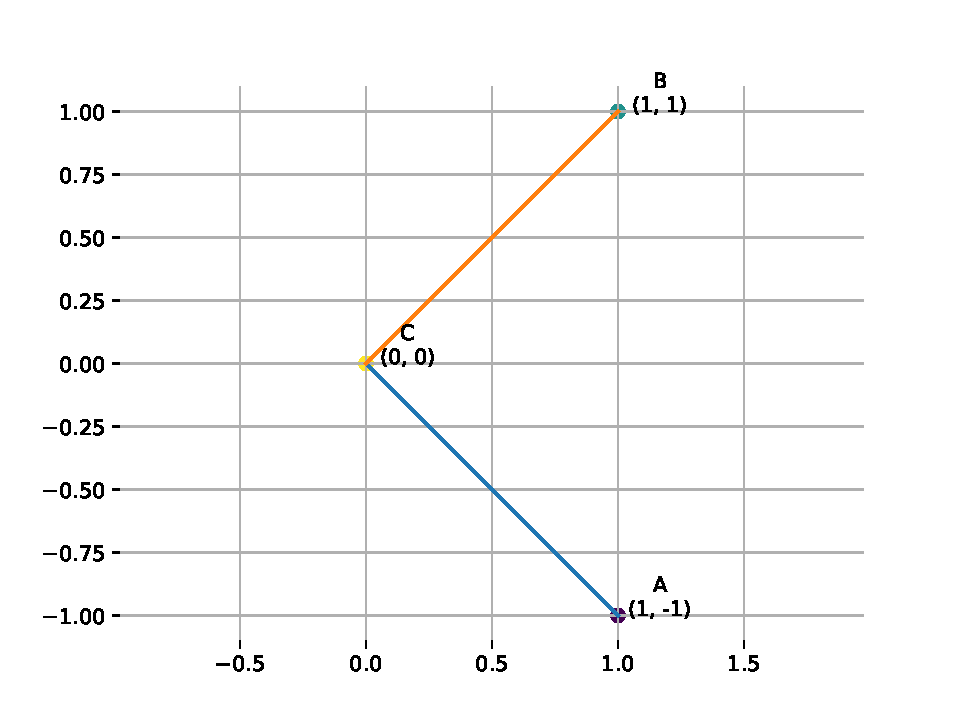
\includegraphics[width=0.75\columnwidth]{chapters/12/10/3/3/figs/fig.pdf}
\caption{}
		\label{fig:12/10/3/3fig}
\end{figure}

\item Show that each of the given three vectors is a unit vector: 
 $\frac{1}{7}(2\hat{i}+3\hat{j}+6\hat{k}),\frac{1}{7}(3\hat{i}-6\hat{j}+2\hat{k}),\frac{1}{7}(6\hat{i}+2\hat{j}-3\hat{k}$).
Also,show that they are mutually perpendicular to each other.
	\\
	\solution
		\begin{align}
\vec{A} = 	\myvec{
	\frac{2}{7} & \frac{3}{7} & \frac{6}{7} \\[1ex]
    \frac{3}{7} & -\frac{6}{7} & \frac{2}{7} \\[1ex]
    \frac{6}{7} & \frac{2}{7} & -\frac{3}{7}
}
\end{align}
is an orthogonal matrix satisfying
\eqref{eq:12/10/3/5/inner},
which verifies the given conditions.

\item Show that the vectors $2\hat{i}-\hat{j}+\hat{k},\hat{i}-3\hat{j}-5\hat{k}$ and  $3\hat{i}-4\hat{j}-4\hat{k}$ from the vertices of a right angled triangle.
	\\
	\solution
		\begin{align}
\vec{A} = \myvec{2\\-1\\1}, \, \vec{B} = \myvec{1\\-3\\-5}, \, \vec{C}=\myvec{3\\-4\\-4},
\\
\implies \vec{B}-\vec{C} = \myvec{-2\\1\\-1} ,\, 
\vec{C}-\vec{A} = \myvec{1\\-3\\-5} ,\, 
\\
	\text{or, }
\brak{\vec{B}-\vec{C}}^{\top}\brak{\vec{C}-\vec{A}} = 0
\end{align}

\item Show that the points A, B and C with position vectors, $3\hat{i}-4\hat{j}-4\hat{k}, 2\hat{i}-\hat{j}+\hat{k}$ and $\hat{i}-3\hat{j}-5\hat{k}$, respectively, form the vertices of a right angled
triangle.
\\
\solution
		    \begin{align}
         \vec{B} - \vec{A} = \myvec{-1\\3\\5},\, 
         \vec{C} - \vec{B} = \myvec{-1\\-2\\-6},\,
         \vec{C} - \vec{A} = \myvec{-2\\1\\-1},
        \label{eq:chapters/12/10/2/17/dir-vec}
	\\
	    \implies 
	    \brak{\vec{B} - \vec{A}}^\top
	    \brak{\vec{C} - \vec{A}} = 0
    \end{align}
Hence, $\triangle ABC$ is right angled at $\vec{A}$. 

\item Let $\vec{a}=\hat{i}+4\hat{j}+2\hat{k}, \vec{b}=3\hat{i}-2\hat{j}+7\hat{k}$ and $\vec{c}=2\hat{i}-\hat{j}+4\hat{k}$. Find a vector $\vec{d}$ which is perpendicular to both $\vec{a}$ and $\vec{b}$, and $\vec{c}\cdot \vec{d}$=15.\\
	\solution
		From the given information, 
\begin{align}
\vec{a}^{\top}\vec{d} &= 0\\
\vec{b}^{\top}\vec{d} &= 0\\
\vec{c}^{\top}\vec{d} &= 15
\end{align}
yielding
\begin{align}
\myvec{\vec{a}^{\top} \\\vec{b}^{\top}\\\vec{c}^{\top}}\vec{d} &= \myvec{0\\0\\15}\\
\implies \myvec{1&4&2 \\3&-2&7 \\2&-1&4}\vec{d} &= \myvec{0\\0\\15}
\label{eq:chapters/12/10/5/12/1}
\end{align}
%
Forming the augmented matrix, 
\begin{align}
	\myvec{1&4&2&\vrule&0\\ 3&-2&7&\vrule&0 \\ 2&-1&4&\vrule&15} 
	\xleftrightarrow[R_3\leftarrow R_3-2R_1]{R_2\leftarrow R_2-3R_1}
	\myvec{1&4&2&\vrule&0\\ 0&-14&1&\vrule&0 \\ 0&-9&0&\vrule&15}
\nonumber	\\
	\xleftrightarrow[]{R_3\leftarrow R_3-\frac{9}{14}R_2}
	\myvec{1&4&2&\vrule&0\\ 0&-14&1&\vrule&0 \\ 0&0&-\frac{9}{14}&\vrule&15}
	\label{eq:chapters/12/10/5/12/2}
\end{align}
yielding
%
\begin{align}
	\vec{d} &= \myvec{\frac{160}{3}\\[1ex]-\frac{5}{3}\\[1ex]-\frac{70}{3}}
\end{align}
upon back substitution.


\item $ABCD$ is a rectangle formed by the points $\vec{A}(–1, –1), \vec{B}(– 1, 4), \vec{C}(5, 4)$  and  $\vec{D}(5, – 1)$. $\vec{P}, \vec{Q}, \vec{R}$ and $\vec{S}$ are the mid-points of $AB, BC, CD$ and $DA$ respectively. Is the quadrilateral $PQRS$ a square? a rectangle? or a rhombus? Justify your answer.
	\\
	\solution 
See Fig. \ref{fig:10/7/4/8Fig3}. From 
  \eqref{eq:10/7/4/8det2f}, $PQRS$ is a parallelogram.
\begin{align}
  %\label{eq:10/7/4/8det2f}
  \vec{P}  = 
 \frac{3}{2},\, 
 \vec{Q}  = \myvec{
 2 \\
 4 \\
 } ,\,
 \vec{R}  = \myvec{
 5 \\
 \frac{3}{2}
 }   
  ,\,
 \vec{S}  = \myvec{
 2\\
 -1 \\
 }   
 \\
	\implies 
 \brak{\vec{Q}-\vec{P}}^\top\brak{\vec{R}-\vec{Q}}  \neq 0
 \\
 \brak{\vec{R}-\vec{P}}^\top\brak{\vec{S}-\vec{Q}}  = 0
\end{align}
Therefore $PQRS$ is a rhombus.
\begin{figure}[!h]
	\begin{center}
		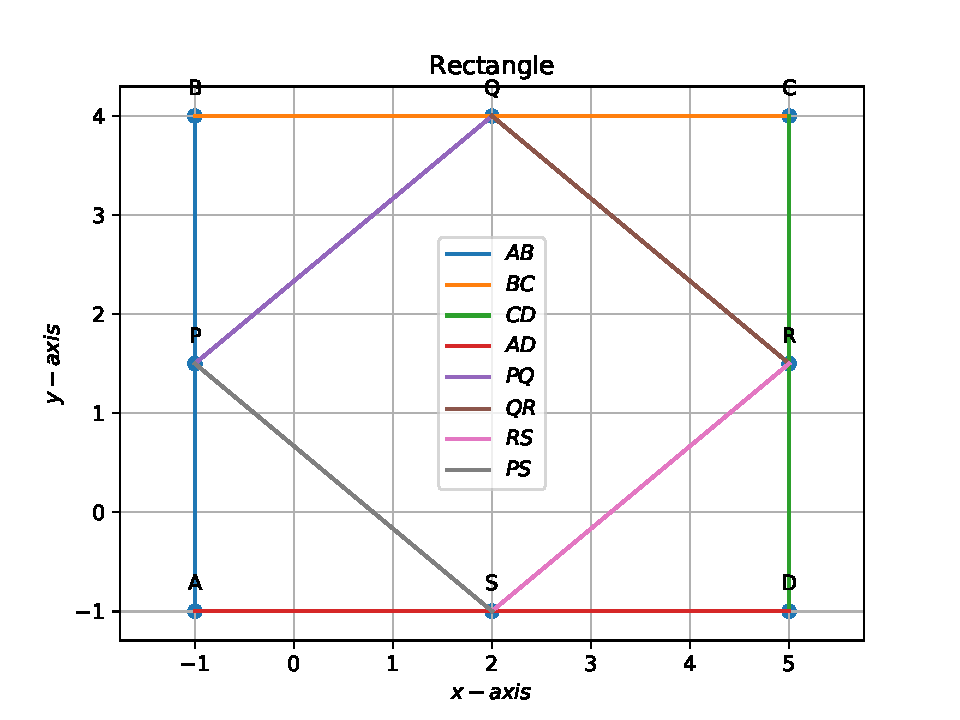
\includegraphics[width=\columnwidth]{chapters/10/7/4/8/figs/problem1.pdf}
	\end{center}
\caption{}
\label{fig:10/7/4/8Fig3}
\end{figure}


\item Without using the Baudhayana theorem, show that the points $A(4,4), B(3,5)$ and $C(-1,-1)$ are the vertices of a right angled triangle.
\label{chapters/11/10/1/6}
		See \figref{fig:11/10/1/6}.
\begin{align}
	\vec{C}-\vec{A}=\myvec{
-5 \\
	-5},\,
	\vec{A}-\vec{B}&=\myvec{
1 \\
-1 
}
\\
	\implies \brak{\vec{C}-\vec{A}}^{\top}
	\brak{\vec{A}-\vec{B}}&=0
\end{align}
Thus, $AB \perp AC$.
	\begin{figure}[H]
		\centering
 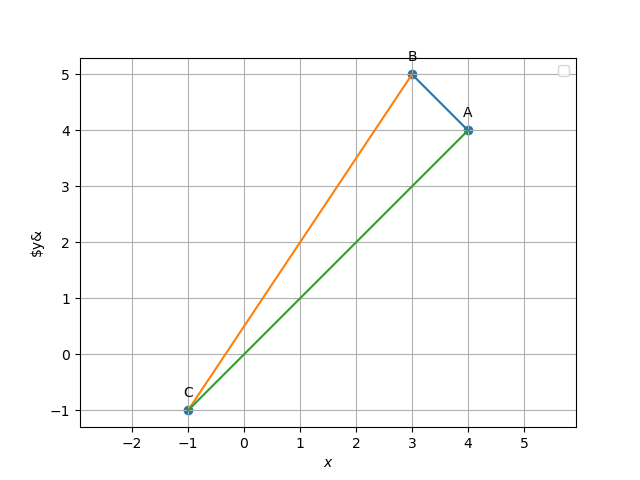
\includegraphics[width=0.75\columnwidth]{chapters/11/10/1/6/figs/triangle.png}
		\caption{}
		\label{fig:11/10/1/6}
  	\end{figure}

\item The line through the points $(h, 3)$ and $(4, 1)$ intersects the line $7x- 9y- 19= 0$ at a right angle. Find the value of $h$.
\label{chapters/11/10/3/10}
\\
\solution
The direction vectors of the given lines are 
\begin{align}
\myvec{4-h\\ -2}
,\,
\myvec{9\\ 7}
\\
\implies 
\myvec{9& 7}\myvec{4-h\\ -2}=0\\
\implies h=\frac{22}{9}
\end{align}
See  
		\figref{fig:chapters/11/10/3/10/Figure}.
\begin{figure}[h]
\centering
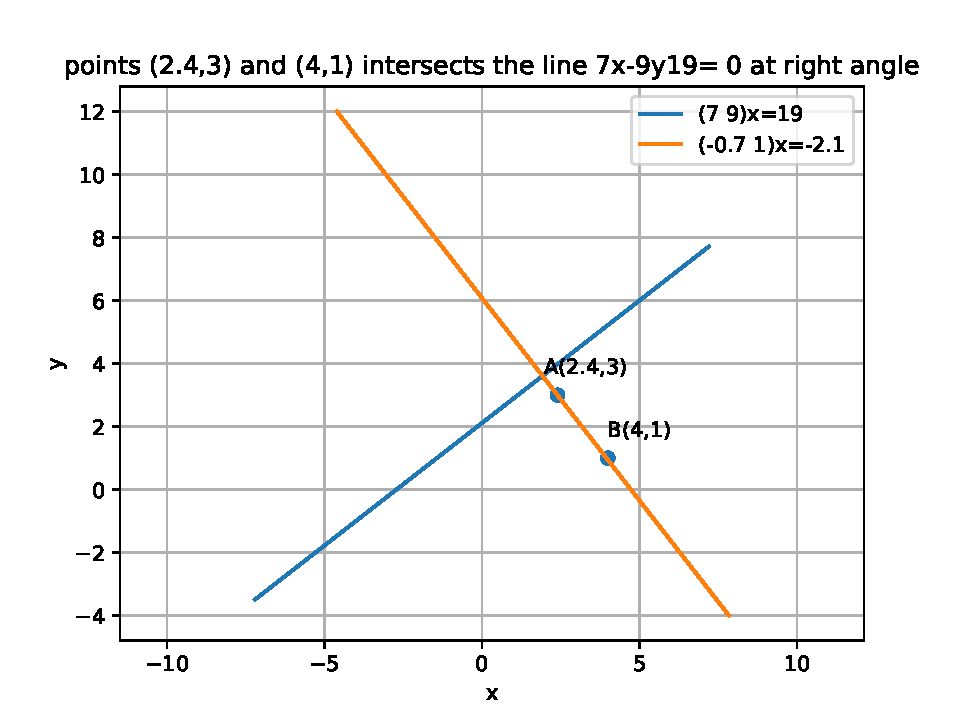
\includegraphics[width=\columnwidth]{chapters/11/10/3/10/figs/fig.pdf}
\caption{}
		\label{fig:chapters/11/10/3/10/Figure}
\end{figure}

\item In the following cases, determine whether the given planes are parallel or perpendicular, and in case they are neither, find the angles between them.
\begin{enumerate}
\item $7x + 5y + 6z + 30 = 0$ and $3x – y – 10z + 4 = 0$
\item $2x + y + 3z – 2 = 0$ and $x – 2y + 5 = 0$
\item $2x – 2y + 4z + 5 = 0$ and $3x – 3y + 6z – 1 = 0$
\item $2x – y + 3z – 1 = 0$ and $2x – y + 3z + 3 = 0$
\item $4x + 8y + z – 8 = 0$ and $y + z – 4 = 0$
\end{enumerate}
    \solution
		    See \tabref{tab:12/11/3/13}.
\begin{table}[htbp]
    \centering
    \caption{}
    \label{tab:12/11/3/13}
    \begin{tabular}{|c|c|c|c|c|c|}
        \hline
        $\vec{n}_1$ & $\vec{n}_1$ & $\vec{n}_1^{\top}\vec{n}_2$ & $\norm{\vec{n}_1}$ & $\norm{\vec{n}_2}$ & Angle\\
        \hline
        $\myvec{7\\5\\6}$ & $\myvec{3\\-1\\-10}$ & $-44$ & $\sqrt{110}$ & $\sqrt{110}$ & $\cos^{-1}-\frac{2}{5}$ \\
        \hline
        $\myvec{2\\1\\3}$ & $\myvec{1\\-2\\0}$ & $0$ & & & perpendicular \\
        \hline
        $\myvec{2\\-2\\4}$ & $\myvec{3\\-3\\6}$ & $36$ & $\sqrt{24}$ & $\sqrt{54}$ & parallel \\
        \hline
        $\myvec{2\\-1\\3}$ & $\myvec{2\\-1\\3}$ & $14$ & $\sqrt{14}$ & $\sqrt{14}$ & parallel \\
        \hline
        $\myvec{4\\8\\1}$ & $\myvec{0\\1\\1}$ & $9$ & $9$ & $\sqrt{2}$ & $45\degree$ \\
        \hline
    \end{tabular}
\end{table}

\iffalse
\begin{table}[htbp]
    \centering
    \caption{}
    \label{}
    \begin{tabular}{|c|c|c|c|c|c|}
        \hline
	    $\vec{n}_1$ & $\vec{n}_1$ &  $\vec{n}_1^{\top}\vec{n}_2$& $\norm{\vec{n}_1}$ &$\norm{\vec{n}_2}$  &  Angle\\
        \hline
	    \myvec{7\\5\\6} & \myvec{3\\-1\\-10} & -44 & \sqrt{110} &\sqrt{110}  & \cos^{-1}-\frac{2}{5} \\
        \hline
\myvec{2\\1\\3}  & \myvec{1\\-2\\0}& 0 &  &  & perpendicular\\
        \hline
 \myvec{2\\-2\\4} & \myvec{3\\-3\\6} & 36  & \sqrt{24} & \sqrt{54} &  parallel \\
        \hline
 \myvec{2\\-1\\3} & \myvec{2\\-1\\3} & 14 & \sqrt{14} & \sqrt{14} & parallel \\
        \hline
 \myvec{4\\8\\1} & \myvec{0\\1\\1} & 9 & 9 & \sqrt{2} &  45\degree  \\
        \hline
    \end{tabular}
\end{table}
\fi

		\item 
 Show that the line joining the origin to the point $P(2, 1, 1)$ is perpendicular to the
line determined by the points $A(3, 5, – 1), B(4, 3, – 1)$.
\\
    \solution
				\begin{align}
			\brak{\vec{A}-\vec{B}}^\top\vec{P}=
			\myvec{-1&2&0}\myvec{2\\1\\1}=0 \qed
		\end{align}

	\item If the lines $\frac{x-1}{-3} = \frac{y-2}{2k} = \frac{z-3}{2}$ and  $\frac{x-1}{3k} = \frac{y-1}{1} = \frac{z-6}{-5}$ are perpendicular, find the value of $k$.\\
    \solution
		From the given information,
\begin{align}
\vec{m}_1 = \myvec{-3\\ 2k\\ 2},\,  \vec{m}_2 =\myvec{3k\\ 1\\ -5} 
\\
	\implies \myvec{-3& 2k& 2}^{\top} \myvec{3k\\ 1\\ -5} =0
	\\
	\implies k = -\frac{10}{7}
\end{align}
See 
     \figref{fig:chapters/12/11/4/6/1}
\begin{figure}[h!]
  \centering
   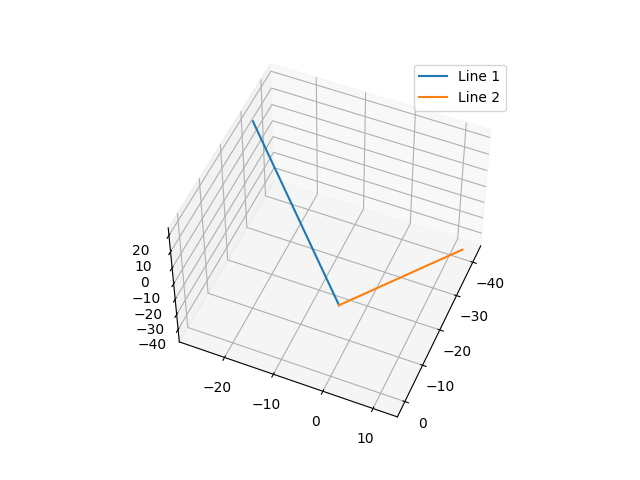
\includegraphics[width=\columnwidth]{chapters/12/11/4/6/figs/line_1.png}
    \caption{lines represented for the given points and direction vector with k=$\frac{-10}{7}$}
     \label{fig:chapters/12/11/4/6/1}
     \end{figure}  



\item Find a unit vector perpendicular to each of the vector $\overrightarrow{a}+\overrightarrow{b}\text{ and }\overrightarrow{a}-\overrightarrow{b},\text{ where } \overrightarrow{a}=3\hat{i}+2\hat{j}+2\hat{k}\text{ and } \overrightarrow{b}=\hat{i}+2\hat{j}-2\hat{k}$. 
	\\
		\solution
		Let the desired vector be $\vec{x}$.  Then, 
\begin{align} 
\myvec{\vec{a}+\vec{b}& \vec{a}-\vec{b}}^\top\vec{x}=0\\
	\label{eq:12/10/4/2/given}
\end{align}
\begin{align}
	\because 
	\vec{a}+\vec{b}= \myvec{\vec{a} & \vec{b}}\myvec{1 \\ 1}
	\\
	\vec{a} - \vec{b}= \myvec{\vec{a} & \vec{b}}\myvec{1 \\ -1}, 
\end{align}
	\eqref{eq:12/10/4/2/given}
	can be expressed as 
\begin{align}
	\cbrak{\myvec{\vec{a} & \vec{b}}\myvec{1 & 1\\ 1 & -1}}^\top\vec{x}=0\\
\implies 	\myvec{1 & 1\\ 1 & -1}^\top\myvec{\vec{a} & \vec{b}}^\top\vec{x}=0
\\
\implies 	\myvec{1 & 1\\ 1 & -1}\myvec{1 & 1\\ 1 & -1}^\top\myvec{\vec{a} & \vec{b}}^\top\vec{x}=0
\\
	\text{or, }
\myvec{\vec{a} & \vec{b}}^\top\vec{x}=0
\end{align}
which can be expressed as 
\begin{align} 
\myvec{
3&2&2\\
1&2&-2
}
	\xleftrightarrow[R_2 = \frac{R_2}{4}]{R_2=3R_2-R_1}
\myvec{
3&2&2\\
0&1&-2
	}
	\\
	\xleftrightarrow[R_1 = \frac{R_1}{3}]{R_1=R_1 - 2R_2}
\myvec{
1&0&2\\
0&1&-2
}
\end{align}
yielding
\begin{align}
\begin{split}
x_1+2x_3=0\\
x_2-2x_3=0
\end{split}
\implies 
\vec{x}
=x_3\myvec{-2\\2\\1}
\end{align}
Thus, the desired unit vector  is 
\begin{align}
\vec{x}
	=\frac{1}{3}\myvec{-2\\2\\1}
\end{align}

\item If $\overrightarrow {a}=2\hat{i}+2\hat{j}3\hat{k},\overrightarrow {b}=\hat{-i}+2\hat{j}+\hat{k}$ and $\overrightarrow {c}=3\hat{i}+\hat{j}$ are such that $\overrightarrow {a}+\lambda\overrightarrow {b}$ is perpendicular to $\overrightarrow {c}$,then find the value of $\lambda$.
	\\
		\solution
\begin{align}
\because	(\vec{a}+\lambda \vec{b})^{\top} \vec{c} = 0,
	\\
	\lambda=-\frac{\vec{a}^{\top}\vec{c}}{\vec{b}^{\top}\vec{c}}
	=8,
\end{align}
upon substituting numerical values.



\item Check whether $(5,-2), (6,4)$ and $(7,-2)$ are the vertices of an isosceles triangle.
\item The perpendicular bisector of the line segment joining the points $\vec{A} (1, 5) \text{ and }
\vec{B} (4, 6)$ cuts the y-axis at
\begin{enumerate}
	\item$(0, 13)$ 
	\item $(0, –13)$
	\item$(0, 12) $
	\item$(13, 0)$
\end{enumerate}
\item The point which lies on the perpendicular bisector of the line segment joining the
	points $\vec{A} (–2, –5)\text { and } \vec{B} (2, 5) $ is
\begin{enumerate}
\item  	$(0, 0)$
\item  $(0, 2)$ 
\item  $(2, 0)$ 
\item  $(–2, 0)$
\end{enumerate}
\item The points $ (–4, 0), (4, 0), (0, 3) $ are the vertices of
	\begin{enumerate}
\item right triangle 
\item isosceles triangle
\item  equilateral triangle
\item  scalene triangle 
\end{enumerate}
\item The point $\vec{A}(2,7)$ lies on the perpendicular bisector of line segment joining the points $\vec{P}(6,5)\text{ and } \vec{Q}(0,-4)$.
\item The points $\vec{A}(-1,-2), \vec{B}(4,3), \vec{C}(2,5) \text{ and } \vec{D}(-3,0)$ in that order form a rectangle.
\item Name the type of triangle formed by the points $\vec{A}(-5,6),\vec{B}(-4,-2),\text{ and }\vec{C}(7,5)$.
\item What type of a quadrilateral do the points $\vec{A}(2,-2),\vec{B}(7,3),\vec{C}(11,-1),\text{ and }\vec{D}(6,-6)$ taken in that order, form?
\item Find the coordinates of the point $\vec{Q}$ on the $x$-axis which lies on the perpendicular bisector of the line segment joining the points $\vec{A}(-5,-2) \text{ and } \vec{B}(4,-2)$. Name the type of triangle formed by points $\vec{Q},\vec{A}\text{ and }\vec{B}$.
\item The points $\vec{A}(2,9),\vec{B}(a,5) \text{ and }\vec{C}(5,5)$ are the vertices of a triangle $\vec{ABC}$ right angled at $\vec{B}$. Find the values of a and hence the area of $\triangle \vec{ABC}$.
\item Find a vector of magnitude 6, which is perpendicular to both the vectors $2\hat{i}-\hat{j}$+$2\hat{k}\text{ and }4\hat{i}-\hat{j}+3\hat{k}$.
\item If A,B,C,D  are the points with position vectors $\hat{i}+\hat{j}-\hat{k}$, $2\hat{i}-\hat{j}+3\hat{k}$, $2\hat{i}-3\hat{k}$, $3\hat{i}$-$2\hat{j}$+$\hat{k}$, respectively, find the projection of $\overline{AB}$ $\text{ along }$ $\overline{CD}$.
\item Find the value of $\lambda$ such that the vectors $\vec{a}=2\hat{i}+\lambda\hat{j}+\hat{k}$ $\text{and}$ $\vec{b}=\hat{i}+2\hat{j}+3\hat{k}$ are orthogonal.
	\begin{enumerate}
\item 0
\item 1 
\item $\frac{3}{2}$
\item $-\frac{5}{2}$
	\end{enumerate}
\item The number of vectors of unit length perpendicular to the vectors $\vec{a}=2\hat{i}+\hat{j}+2\hat{k}$ $\text{ and }$ $\vec{b}=\hat{j}+\hat{k}$ is
	\begin{enumerate}
\item one
\item  two
\item three
\item infinite
\end{enumerate}
\item Find the equation of a plane which  bisects perpendicularly the line joining the points A$(2,3,4)$ and B$(4,5,8)$ at right angles.
\item $\overrightarrow{AB}=3\hat{i}-\hat{j}+\hat{k}$ and $\overrightarrow{CD}=-3\hat{i}+2\hat{j}+4\hat{k}$ are two vectors. The position vectors of the points A and C are $6\hat{i}+7\hat{j}+4\hat{k}$ and $-9\hat{j}+2\hat{k},$ respectively. Find the position vector of a point P on the line AB and a point Q on the line CD such that $\overrightarrow{PQ}$ is perpendicular to $\overrightarrow{AB}$ and $\overrightarrow{CD}$ both.
\item Line joining the points (3,-4) and (-2,6) is perpendicular to the line joining the points (-3,6) and (9,-18).
\item Verify the following:
\begin{enumerate}
\item $(0,7,-10), (1,6,-6)$ and $(4,9,-6)$ are the vertices of an isoceles triangle.
\item $(0,7,10), (-1,6,6)$ and $(-4,9,6)$ are the vertices of a right angled triangle.
\end{enumerate}
\end{enumerate}

\subsection{CBSE}
\begin{enumerate}[label=\thesubsection.\arabic*, ref=\thesubsection.\theenumi]
\item Show that the points \brak{7, 10}, \brak{-2, 5} and \brak{3, 4} are vertices of an isosceles right triangle.
The points form an isosceles right triangle.
\hfill (10, 2020)
    \item The points $(-4,0)$, $(4,0)$, and $(0,3)$ are the vertices of a:
    \begin{enumerate}
        \item right triangle
        \item isosceles triangle
        \item equilateral triangle
        \item scalene triangle
    \end{enumerate}
    \hfill (10, 2023)
    \item Show that the points $(-2,3)$, $(8,3)$, and $(6,7)$ are the vertices of a right-angled triangle.
    \hfill (10, 2023)
    \item If
    \begin{align}
        \overrightarrow{a} = 2\hat{i} + y\hat{j} + \hat{k}
    \end{align}
    and
    \begin{align}
        \overrightarrow{b} = \hat{i} + 2\hat{j} + 3\hat{k}
    \end{align}
    are two vectors for which the vector $(\overrightarrow{a} + \overrightarrow{b})$ is perpendicular to the vector $(\overrightarrow{a} - \overrightarrow{b})$, then find all the possible values of $y$.
    \hfill (12, 2023)
    \item Write the projection of the vector $(\overrightarrow{b} + \overrightarrow{c})$ on the vector $\overrightarrow{a}$, where
    \begin{align}
        \overrightarrow{a} = 2\hat{i} - 2\hat{j} + \hat{k},
    \end{align}
    \begin{align}
        \overrightarrow{b} = \hat{i} + 2\hat{j} - 2\hat{k},
    \end{align}
    and
    \begin{align}
        \overrightarrow{c} = 2\hat{i} - \hat{j} + 4\hat{k}.
    \end{align}
    \hfill (12, 2023)

    \item If
    \begin{align}
        \overrightarrow{a} = 2\hat{i} - \hat{j} + \hat{k},
    \end{align}
    \begin{align}
        \overrightarrow{b} = \hat{i} + \hat{j} - 2\hat{k},
    \end{align}
    and
    \begin{align}
        \overrightarrow{c} = \hat{i} + 3\hat{j} - \hat{k},
    \end{align}
    and the projection of vector $\overrightarrow{c} + \lambda \overrightarrow{b}$ on vector $\overrightarrow{a}$ is $2\sqrt{6}$, find the value of $\lambda$.
    \hfill (12, 2023)
    \item If
    \begin{align}
        \overrightarrow{a} = 2\hat{i} - \hat{j} + 2\hat{k},
    \end{align}
    and
    \begin{align}
        \overrightarrow{b} = 5\hat{i} - 3\hat{j} - 4\hat{k},
    \end{align}
    then find the ratio of the projection of vector $\overrightarrow{a}$ on vector $\overrightarrow{b}$ to the projection of vector $\overrightarrow{b}$ on vector $\overrightarrow{a}$.
    \hfill (12, 2023)

    \item Show that the three vectors $2\hat{i} - \hat{j} + \hat{k}$, $\hat{i} - 3\hat{j} - 5\hat{k}$, and $3\hat{i} - 4\hat{j} - 4\hat{k}$ form the vertices of a right-angled triangle. 
    \hfill (12, 2023)
    \item If
    \begin{align}
        \overrightarrow{a} = 2\hat{i} + 2\hat{j} + 3\hat{k},
    \end{align}
    \begin{align}
        \overrightarrow{b} = -\hat{i} + 2\hat{j} + \hat{k},
    \end{align}
    and
    \begin{align}
        \overrightarrow{c} = 3\hat{i} + \hat{j},
    \end{align}
    are such that the vector $(\overrightarrow{a} + \lambda \overrightarrow{b})$ is perpendicular to vector $\overrightarrow{c}$, then find the value of $\lambda$.
    \hfill (12, 2023)
		\item What kind of triangle is formed with vertices $\vec{A}(0, 2)$, $\vec{B}(-3, 0)$, and $\vec{C}(3, 0)$?
		\hfill (10, 2021)
		\begin{enumerate}
			\item A right triangle
			\item An equilateral triangle
			\item An isosceles triangle
			\item A scalene triangle
		\end{enumerate}
		\item Check whether the points $\vec{P}(5, -2)$, $\vec{Q}(6, 4)$, and $\vec{R}(7, -2)$ are the vertices of an isosceles triangle $\triangle PQR$. \hfill (10, 2021)
		\item The points $\vec{A}(0, 3)$, $\vec{B}(-2, a)$, and $\vec{C}(-1, 4)$ are the vertices of a right triangle, right-angled at $\vec{A}$. Find the value of $a$. \hfill (10, 2021)
	\item If $\vec{a} = 2\hat{i} - \hat{j} + 2\hat{k}$ and $\vec{b} = 5\hat{i} - 3\hat{j} - 4\hat{k}$, then find the ratio $\frac{\text{projection of vector } \vec{a} \text{ on } \vec{b}}{\text{projection of vector } \vec{b} \text{ on vector } \vec{a}}$. \hfill (12, 2021)
	\item Let $\hat{a}$ and $\hat{b}$ be two unit vectors. If the vectors $\vec{c} = \hat{a} + 2\hat{b}$ and $\vec{d} = 5\hat{a} - 4\hat{b}$ are perpendicular to each other, then find the angle between the vectors $\hat{a}$ and $\hat{b}$. \hfill (12, 2021)
%	
	\item Show that $\abs{\vec{a}} \vec{b} + \abs{\vec{b}} \vec{a}$ is perpendicular to $\abs{\vec{a}} \vec{b} - \abs{\vec{b}} \vec{a}$, for any two non-zero vectors $\vec{a}$ and $\vec{b}$. \hfill (12, 2021)
	\item Find the value of $p$ for which the following lines are perpendicular:
	\begin{align*}
	\dfrac{1-x}{3} = \dfrac{2y-14}{2p} = \dfrac{z-3}{2}; \quad \dfrac{1-x}{3p} = \dfrac{y-5}{1} = \dfrac{6-z}{5}.
	\end{align*} \hfill (12, 2019)
%	
	\item Show that the vectors $\hat{i} - 2\hat{j} + 3\hat{k}$, $-2\hat{i} + 3\hat{j} - 4\hat{k}$, and $\hat{i} - 3\hat{j} + 5\hat{k}$ are coplanar. \hfill (12, 2019)
	\item Find a unit vector perpendicular to both the vectors $\overrightarrow{a}$ and $\overrightarrow{b}$, where $\overrightarrow{a} = \hat{i} - 7\hat{j} + 7\hat{k}$ and $\overrightarrow{b} = 3\hat{i} - 2\hat{j} + 2\hat{k}$. \hfill (12, 2019)
	\item Let $\overrightarrow{a} = \hat{i} + 2\hat{j} - 3\hat{k}$ and $\overrightarrow{b} = 3\hat{i} - \hat{j} + 2\hat{k}$. Show that the vectors $\overrightarrow{a} + \overrightarrow{b}$ and $\overrightarrow{a} - \overrightarrow{b}$ are perpendicular to each other. \hfill (12, 2019)
\item Show that the vectors $\hat{i} - 2\hat{j} + 3\hat{k}$, $2\hat{i} + 3\hat{j} - 4\hat{k}$, and $\hat{i} - 3\hat{j} + 5\hat{k}$ are coplanar. \hfill (12, 2018)
\item Find the value of $P$ for which the following lines are perpendicular:
\begin{align*}
\frac{1 - x}{3} &= \frac{2y - 14}{2P} = \frac{z - 3}{2}
\end{align*}
\begin{align*}
\frac{1 - x}{3P} &= \frac{y - 5}{1} = \frac{6 - z}{5}
\end{align*}
\hfill (12, 2018)
\item Find the value of $x$ such that the four points with position vectors $\mathbf{A}(3\hat{i} + 2\hat{j} + \hat{k})$, $\mathbf{B}(4\hat{i} + x\hat{j} + 5\hat{k})$, $\mathbf{C}(4\hat{i} + 2\hat{j} - 2\hat{k})$, and $\mathbf{D}(6\hat{i} + 5\hat{j} - \hat{k})$ are coplanar. \hfill (12, 2018)
 \item Let $\overrightarrow{a}$, $\overrightarrow{b} $ and $\overrightarrow{c}$ be three vectors such that $\abs{\overrightarrow{a}}=1$, $\abs {\overrightarrow{b}}=2 $ and $\abs{\overrightarrow{c}}=3$. If the projection of $\overrightarrow{b}$ along $\overrightarrow{a}$ is equal to the projection of $\overrightarrow{c}$ along $\overrightarrow{a}$ ; and $\overrightarrow{b}$, $\overrightarrow{c}$ are perpendicular to each other, then find $\abs{3\overrightarrow{a}- 2\overrightarrow{b} +2\overrightarrow{c}}$.
\hfill (12, 2018)
\item Find the value of $P$ for which the following lines are perpendicular:
 \begin{align*}
 \frac{1-x}{3}=\frac{2y-14}{2p}=\frac{z-3}{2}; \frac{1-x}{3p}=\frac{y-5}{1}=\frac{6-z}{5}
 \end{align*}
 \hfill (12, 2018)
\item Find the value of $x$, for which the four points $\mathbf{A}\brak{x,1,-1}$, $\mathbf{B}\brak{4,5,1}$, $\mathbf{C}\brak{3,9,4}$ and $\mathbf{D}\brak{-4,4,4}$ are coplanar.
\hfill (12, 2018)
\item Let $\vec{a}=\hat{i}+\hat{2j}-\hat{3k}$ and $\vec{b}=\hat{3i}-\hat{j}+\hat{2k}$ be two vectors. Show that the vectors $(\vec{a}+\vec{b})$ and $(\vec{a}-\vec{b})$ are perpendicular to each other.
\hfill (12, 2018)
\item Using vectors, find the value of $x$ such that the four points $\mathbf{A}$ $\brak{x,5,-1}$,$\mathbf{B}$ $\brak{3,2,1}$,$\mathbf{C}$ $\brak{4,5,5}$ and $\mathbf{D}$ $\brak{4,2,-2}$ are coplanar.

\hfill (12, 2018) 
\item Find the angle between the line $\overrightarrow{r}=\brak{2\hat{i}-\hat{j}+3\hat{k}}+\lambda\brak{3\hat{i}-\hat{j}+2\hat{k}}$ and the plane $\overrightarrow{r}.\brak{\hat{i}+\hat{j}+\hat{k}}=3$.

\hfill (12, 2018) 
\item If $\abs{\overrightarrow{a}}=2$, $\abs{\overrightarrow{b}}=7$ and  $\overrightarrow{a}$ $X$ $\overrightarrow{b} =\hat{3i}+\hat{2j}+\hat{6k}$, find the angle between $\overrightarrow{a}$ and $\overrightarrow{b}$.
\hfill (12, 2018) 
    \item If $\vec{a} = 2\hat{i} - \hat{j} - 2\hat{k}$ and $\vec{b} = 7\hat{i} + 2\hat{j} - 3\hat{k}$, then express $\vec{b}$ in the form $\vec{b} = \vec{b_1} + \vec{b_2}$, where $\vec{b_1}$ is parallel to $\vec{a}$ and $\vec{b_2}$ is perpendicular to $\vec{a}$. \hfill (12, 2017)
    \item Prove that the points $\myvec{3,0}$, $\myvec{6,4}$, and $\myvec{-1,3}$ are the vertices of a right-angled isosceles triangle. \hfill (10, 2016)
\item Write the number of vectors of unit length perpendicular to both the vector
      \begin{align*}
          \vec{a} & = 2 \hat{i} + \hat{j} +2\hat{k} \quad\text{ and} \\
          \vec{b} & = \hat{j}+\hat{k}.
      \end{align*} \hfill (12, 2016)
\item Find the projection of the vector $\vec{a}=2\vec{i}+3\vec{j}+2\vec{k}$ on the vector $\vec{b}=2\vec{i}+2\vec{j}+\vec{k}$. \hfill (12, 2015)
\item The points $\vec{A}\brak{4, 7}$, $\vec{B}\brak{p, 3}$ and $\vec{C}\brak{7, 3}$ are the vertices of a right triangle, right-angled at $\vec{B}$. Find the value of $p$. \hfill (10, 2015)
\item If the two lines
\begin{align}
      L_1 : x=5,\frac{y}{3-\alpha}=\frac{z}{-2}\\
     L_2 : x=2,\frac{y}{-1}=\frac{z}{z-\alpha} 
   \end{align}
are perpendicular, then the value of $\alpha$ 
\hfill (12, 2021)
\end{enumerate}

\subsection{Vector Product}
\begin{enumerate}[label=\thesubsection.\arabic*,ref=\thesubsection.\theenumi]
		\item Find $\abs{\overrightarrow{a}\times\overrightarrow{b}},\text{ if }\overrightarrow{a}=\hat{i}-7\hat{j}+7\hat{k}\text{ and } \overrightarrow{b}=3\hat{i}-2\hat{j}+2\hat{k}$.
	\\
		\solution
		\iffalse
\documentclass[12pt]{article}
\usepackage{graphicx}
\usepackage[none]{hyphenat}
\usepackage{listings}
\usepackage[english]{babel}
\usepackage{booktabs}
\usepackage{caption}
\usepackage{booktabs}
\usepackage{array}
\usepackage{commath}
\usepackage{amssymb}
\usepackage{amsmath}
%\usepackage{extarrows}
\usepackage{commath}
%\usepackage[utf8]{inputenc}
\lstset{ language=tex,
	frame=single,
         breaklines=true
        }
        \usepackage{hyper ref}
        \usepackage{atbegshi}
        \AtBeginDocument{\AtBeginShipoutNext{\AtBeginShipoutDiscard}}

        \newcommand{\mydet}[1]{\ensuremath{\begin{vmatrix}#1\end{vmatrix}}}
        \providecommand{\abs}[1]{\left\vert#1\right\vert}
        \providecommand{\brak}[1]{\ensuremath{\left(#1\right)}}
\providecommand{\norm}[1]{\left\lVert#1\right\rVert}
\newcommand{\solution}{\noindent \textbf{Solution: }}
\newcommand{\myvec}[1]{\ensuremath{\begin{pmatrix}#1\end{pmatrix}}}
\let\vec\mathbf

\begin{document}
\begin{center}\title{\textbf{Vectors Assignment-1}}
	\date{\vspace{-5ex}}
\maketitle
\end{center}
\setcounter{page}{1}
Section{12${th}$Math- Excercise 12.10.4.1}

\begin{enumerate}
	\item Find $\abs{\vec{a}\times\vec{b}}$, if $\vec{a}=\hat{i}-7\hat{j}+7\hat{k}$ $\text{ and } $ $\vec{b}=3\hat{i}-2\hat{j}+2\hat{k}$

\solution
\fi
Since 
\begin{align}
	\mydet{\vec{A}_{23}&\vec{B}_{23}}&=\mydet{-7 & -2 \\ 7 & 2}=-14+14=0\\
	\mydet{\vec{A}_{31}&\vec{B}_{31}}&=\mydet{1 & 3 \\ 7 & 2}=2-21=-19\\
	\mydet{\vec{A}_{12}&\vec{B}_{12}}&=\mydet{1 & 3 \\ -7 & -2}=-2+21=19,
	\\
	\norm{\vec{a}\times\vec{b}}&=\brak{\mydet{\vec{A}_{23}& \vec{B}_{23} \\ \vec{A}_{31} & \vec{B}_{31} \\ \vec{A}_{12}& \vec{B}_{12}}}
=19\sqrt{2}
\end{align}

\item Find $\lambda$ and $\mu$ if $(2\hat{i}+6\hat{j}+27\hat{k})\times(\hat{i}+\lambda \hat{j} + \mu \hat{k})=\overrightarrow{0}$.
	\\
		\solution
		From 
		 Formula \ref{prop:lin-dep-cross},
performing row reduction, 
\begin{align}
 \myvec{2&6&27 \\ 1& \lambda & \mu}
	\xleftrightarrow{R_{2}\leftarrow 2R_{2}-R_{1}}  	
 \myvec{2&6&27 \\ 0& 2\lambda -6 & 2\mu-27}
\end{align}
For the above matrix to have rank 1,
\begin{align}
	\mu=\frac{27}{2},
	\lambda=3.
\end{align}


\item Find the area of the triangle with vertices $A(1, 1, 2), B(2, 3, 5)$ and $C(1, 5, 5)$.
	\\
		\solution
		\iffalse
\documentclass[journal,12pt,twocolumn]{IEEEtran}
\usepackage{setspace}
\usepackage{gensymb}
\singlespacing
\usepackage[cmex10]{amsmath}
\usepackage{amsthm}
\usepackage{mathrsfs}
\usepackage{txfonts}
\usepackage{stfloats}
\usepackage{bm}
\usepackage{cite}
\usepackage{cases}
\usepackage{subfig}
\usepackage{longtable}
\usepackage{multirow}
\usepackage{enumitem}
\usepackage{mathtools}
\usepackage{steinmetz}
\usepackage{tikz}
\usepackage{circuitikz}
\usepackage{verbatim}
\usepackage{tfrupee}
\usepackage[breaklinks=true]{hyperref}
\usepackage{tkz-euclide}
\usetikzlibrary{calc,math}
\usepackage{listings}
    \usepackage{color}                                            %%
    \usepackage{array}                                            %%
    \usepackage{longtable}                                        %%
    \usepackage{calc}                                             %%
    \usepackage{multirow}                                         %%
    \usepackage{hhline}                                           %%
    \usepackage{ifthen}                                           %%
  %optionally (for landscape tables embedded in another document): %%
    \usepackage{lscape}     
\usepackage{multicol}
\usepackage{chngcntr}
\DeclareMathOperator*{\Res}{Res}
\renewcommand\thesection{\arabic{section}}
\renewcommand\thesubsection{\thesection.\arabic{subsection}}
\renewcommand\thesubsubsection{\thesubsection.\arabic{subsubsection}}

\renewcommand\thesectiondis{\arabic{section}}
\renewcommand\thesubsectiondis{\thesectiondis.\arabic{subsection}}
\renewcommand\thesubsubsectiondis{\thesubsectiondis.\arabic{subsubsection}}

% correct bad hyphenation here
\hyphenation{op-tical net-works semi-conduc-tor}
\def\inputGnumericTable{}                                 %%

\lstset{
frame=single, 
breaklines=true,
columns=fullflexible
}

\begin{document}


\newtheorem{theorem}{Theorem}[section]
\newtheorem{problem}{Problem}
\newtheorem{proposition}{Proposition}[section]
\newtheorem{lemma}{Lemma}[section]
\newtheorem{corollary}[theorem]{Corollary}
\newtheorem{example}{Example}[section]
\newtheorem{definition}[problem]{Definition}
\newcommand{\BEQA}{\begin{eqnarray}}
\newcommand{\EEQA}{\end{eqnarray}}
\newcommand{\define}{\stackrel{\triangle}{=}}

\bibliographystyle{IEEEtran}
\providecommand{\mbf}{\mathbf}
\providecommand{\pr}[1]{\ensuremath{\Pr\left(#1\right)}}
\providecommand{\qfunc}[1]{\ensuremath{Q\left(#1\right)}}
\providecommand{\sbrak}[1]{\ensuremath{{}\left[#1\right]}}
\providecommand{\lsbrak}[1]{\ensuremath{{}\left[#1\right.}}
\providecommand{\rsbrak}[1]{\ensuremath{{}\left.#1\right]}}
\providecommand{\brak}[1]{\ensuremath{\left(#1\right)}}
\providecommand{\lbrak}[1]{\ensuremath{\left(#1\right.}}
\providecommand{\rbrak}[1]{\ensuremath{\left.#1\right)}}
\providecommand{\cbrak}[1]{\ensuremath{\left\{#1\right\}}}
\providecommand{\lcbrak}[1]{\ensuremath{\left\{#1\right.}}
\providecommand{\rcbrak}[1]{\ensuremath{\left.#1\right\}}}
\theoremstyle{remark}
\newtheorem{rem}{Remark}
\newcommand{\sgn}{\mathop{\mathrm{sgn}}}
\providecommand{\abs}[1]{\left\vert#1\right\vert}
\providecommand{\res}[1]{\Res\displaylimits_{#1}} 
\providecommand{\norm}[1]{\left\lVert#1\right\rVert}
\providecommand{\mtx}[1]{\mathbf{#1}}
\providecommand{\mean}[1]{E\left[ #1 \right]}
\providecommand{\fourier}{\overset{\mathcal{F}}{ \rightleftharpoons}}
\providecommand{\system}{\overset{\mathcal{H}}{ \longleftrightarrow}}
\newcommand{\solution}{\noindent \textbf{Solution: }}
\newcommand{\cosec}{\,\text{cosec}\,}
\providecommand{\dec}[2]{\ensuremath{\overset{#1}{\underset{#2}{\gtrless}}}}
\newcommand{\myvec}[1]{\ensuremath{\begin{pmatrix}#1\end{pmatrix}}}
\newcommand{\mydet}[1]{\ensuremath{\begin{vmatrix}#1\end{vmatrix}}}
\numberwithin{equation}{subsection}
\makeatletter
\@addtoreset{figure}{problem}
\makeatother

\let\StandardTheFigure\thefigure
\let\vec\mathbf
\renewcommand{\thefigure}{\theproblem}



\def\putbox#1#2#3{\makebox[0in][l]{\makebox[#1][l]{}\raisebox{\baselineskip}[0in][0in]{\raisebox{#2}[0in][0in]{#3}}}}
     \def\rightbox#1{\makebox[0in][r]{#1}}
     \def\centbox#1{\makebox[0in]{#1}}
     \def\topbox#1{\raisebox{-\baselineskip}[0in][0in]{#1}}
     \def\midbox#1{\raisebox{-0.5\baselineskip}[0in][0in]{#1}}

\vspace{3cm}


\title{Assignment 1}
\author{Jaswanth Chowdary Madala}





% make the title area
\maketitle

\newpage

%\tableofcontents

\bigskip

\renewcommand{\thefigure}{\theenumi}
\renewcommand{\thetable}{\theenumi}

\begin{enumerate}
\item Find the area of the triangle with vertices $\vec{A}$(1,1,2), $\vec{B}$ (2,3,5), $\vec{C}$ (1,5,5).

\textbf{Solution:} The area of the triangle $ABC$ is given by
\begin{align}
ar(ABC) &= \dfrac{1}{2}\norm{\brak{\vec{B}-\vec{A}} \times \brak{\vec{C}-\vec{A}}}
\end{align}


given points are 
\fi
Since
\begin{align}
\vec{B}-\vec{A} = \myvec{1\\2\\3}, 
\vec{C}-\vec{A} = \myvec{0\\4\\3} \\
\end{align}
the desired area is given by 
\begin{align}
	\frac{1}{2} \norm{\myvec{1\\2\\3} \times \myvec{0\\4\\3}} 
	= 	\frac{1}{2}\norm{\myvec{-6\\3\\4}}
= \dfrac{\sqrt{61}}{2}
\end{align}






\item Find the area of the parallelogram whose adjacent sides are determined by the vectors $\overrightarrow{a}=\hat{i}-\hat{j}+3\hat{k}$ and $\overrightarrow{b}=2\hat{i}-7\hat{j}+\hat{k}$.
	\\
		\solution
					From \eqref{eq:tri-area-cross},
			the desired area is obtained as
\begin{align}
	\norm{\myvec{1\\-1\\3} \times \myvec{2\\ -7 \\ 1}}
	=\norm{\myvec{20\\5\\-5}}
= 15\sqrt{2}
\end{align}


\item Find the area of a rhombus if its vertices are $A(3,0), B(4,5), C(-1,4)$  and  $D(-2,-1)$ taken in order. 
	\\
		\solution
	The area of the rhombus is
\begin{align}
                \norm{\myvec{\vec{A-D}}\times \myvec{\vec{B-A}}}=\mydet{5 & 1\\1 & 5} = 24
\end{align}
See 
\figref{fig:chapters/10/7/2/10/gFig1}.
\begin{figure}[!h]
 \begin{center}
  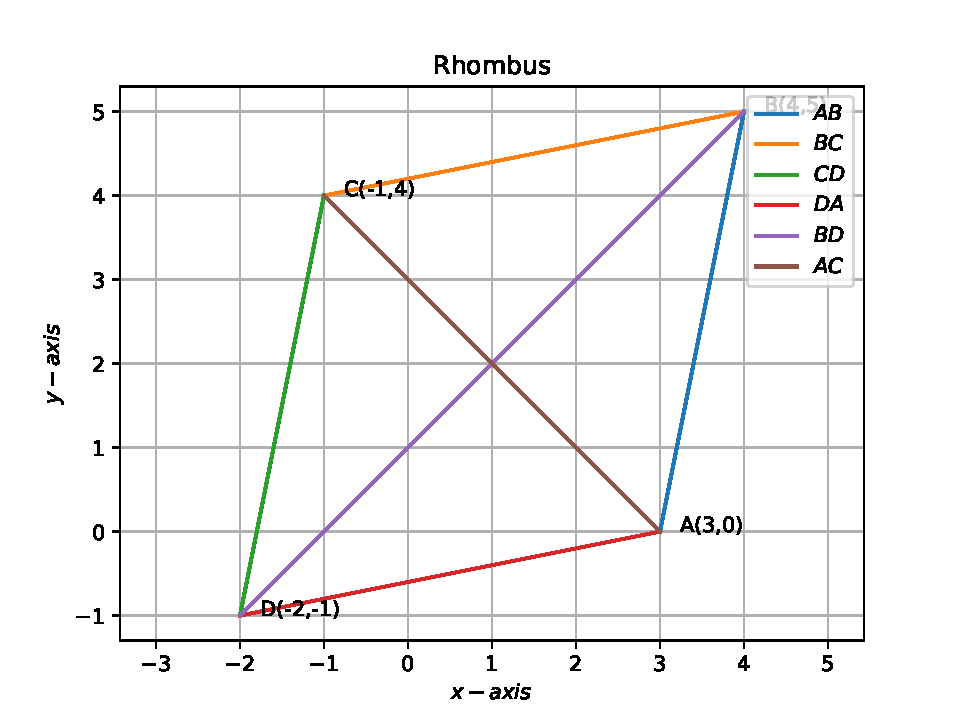
\includegraphics[width=\columnwidth]{chapters/10/7/2/10/figs/fig.pdf}
 \end{center}
\caption{}
\label{fig:chapters/10/7/2/10/gFig1}
\end{figure}

\item Let the vectors $\overrightarrow{a}$ and $\overrightarrow{b}$ be such that $|\overrightarrow{a}| = 3$ and $|\overrightarrow{b}| = \dfrac{\sqrt{2}}{3}$, then $\overrightarrow{a} \times \overrightarrow{b}$ is a unit vector, if the angle between $\overrightarrow{a}$ and $\overrightarrow{b}$ is
\begin{enumerate}
\item $\frac{\pi}{6}$
\item $\frac{\pi}{4}$
\item $\frac{\pi}{3}$
\item $\frac{\pi}{2}$
\end{enumerate}
		\solution
		From the given information and 
	\eqref{eq:cross-sin}
%
\begin{align}
	\norm{\vec{a} \times \vec{b}} & = \norm{\vec{a}} \norm{\vec{b}} \sin \theta =1\\
\implies\sin \theta & = \frac{1} {\norm{\vec{a}} \norm{\vec{b}}}
 = \frac{1}{\sqrt{2}}\\
\implies\theta &= 
 \frac{\pi}{4} 
\end{align}

\item Area of a rectangle having vertices A, B, C and D with position vectors $ -\hat{i}+ \frac{1}{2} \hat{j}+4\hat{k}, \hat{i}+ \frac{1}{2} \hat{j}+4\hat{k}, \hat{i}-\frac{1}{2} \hat{j}+4\hat{k}$ and $-\hat{i}- \frac{1}{2} \hat{j}+4\hat{k}$, respectively is
\begin{enumerate}
\item $\frac{1}{2}$
\item 1
\item 2
\item 4
\end{enumerate}
		\solution
		\iffalse
\documentclass[journal,12pt,twocolumn]{IEEEtran}
%
\usepackage{setspace}
\usepackage{gensymb}
%\doublespacing
\singlespacing

%\usepackage{graphicx}
%\usepackage{amssymb}
%\usepackage{relsize}
\usepackage[cmex10]{amsmath}
%\usepackage{amsthm}
%\interdisplaylinepenalty=2500
%\savesymbol{iint}
%\usepackage{txfonts}
%\restoresymbol{TXF}{iint}
%\usepackage{wasysym}
\usepackage{amsthm}
%\usepackage{iithtlc}
\usepackage{mathrsfs}
\usepackage{txfonts}
\usepackage{stfloats}
\usepackage{bm}
\usepackage{cite}
\usepackage{cases}
\usepackage{subfig}
%\usepackage{xtab}
\usepackage{longtable}
\usepackage{multirow}
%\usepackage{algorithm}
%\usepackage{algpseudocode}
\usepackage{enumitem}
\usepackage{mathtools}
\usepackage{steinmetz}
\usepackage{tikz}
\usepackage{circuitikz}
\usepackage{verbatim}
\usepackage{tfrupee}
\usepackage[breaklinks=true]{hyperref}
%\usepackage{stmaryrd}
\usepackage{tkz-euclide} % loads  TikZ and tkz-base
%\usetkzobj{all}
\usetikzlibrary{calc,math}
\usepackage{listings}
    \usepackage{color}                                            %%
    \usepackage{array}                                            %%
    \usepackage{longtable}                                        %%
    \usepackage{calc}                                             %%
    \usepackage{multirow}                                         %%
    \usepackage{hhline}                                           %%
    \usepackage{ifthen}                                           %%
  %optionally (for landscape tables embedded in another document): %%
    \usepackage{lscape}     
\usepackage{multicol}
\usepackage{chngcntr}
%\usepackage{enumerate}

%\usepackage{wasysym}
%\newcounter{MYtempeqncnt}
\DeclareMathOperator*{\Res}{Res}
%\renewcommand{\baselinestretch}{2}
\renewcommand\thesection{\arabic{section}}
\renewcommand\thesubsection{\thesection.\arabic{subsection}}
\renewcommand\thesubsubsection{\thesubsection.\arabic{subsubsection}}

\renewcommand\thesectiondis{\arabic{section}}
\renewcommand\thesubsectiondis{\thesectiondis.\arabic{subsection}}
\renewcommand\thesubsubsectiondis{\thesubsectiondis.\arabic{subsubsection}}

% correct bad hyphenation here
\hyphenation{op-tical net-works semi-conduc-tor}
\def\inputGnumericTable{}                                 %%

\lstset{
%language=C,
frame=single, 
breaklines=true,
columns=fullflexible
}
%\lstset{
%language=tex,
%frame=single, 
%breaklines=true
%}

\begin{document}
%


\newtheorem{theorem}{Theorem}[section]
\newtheorem{problem}{Problem}
\newtheorem{proposition}{Proposition}[section]
\newtheorem{lemma}{Lemma}[section]
\newtheorem{corollary}[theorem]{Corollary}
\newtheorem{example}{Example}[section]
\newtheorem{definition}[problem]{Definition}
%\newtheorem{thm}{Theorem}[section] 
%\newtheorem{defn}[thm]{Definition}
%\newtheorem{algorithm}{Algorithm}[section]
%\newtheorem{cor}{Corollary}
\newcommand{\BEQA}{\begin{eqnarray}}
\newcommand{\EEQA}{\end{eqnarray}}
\newcommand{\define}{\stackrel{\triangle}{=}}

\bibliographystyle{IEEEtran}
%\bibliographystyle{ieeetr}


\providecommand{\mbf}{\mathbf}
\providecommand{\pr}[1]{\ensuremath{\Pr\left(#1\right)}}
\providecommand{\qfunc}[1]{\ensuremath{Q\left(#1\right)}}
\providecommand{\sbrak}[1]{\ensuremath{{}\left[#1\right]}}
\providecommand{\lsbrak}[1]{\ensuremath{{}\left[#1\right.}}
\providecommand{\rsbrak}[1]{\ensuremath{{}\left.#1\right]}}
\providecommand{\brak}[1]{\ensuremath{\left(#1\right)}}
\providecommand{\lbrak}[1]{\ensuremath{\left(#1\right.}}
\providecommand{\rbrak}[1]{\ensuremath{\left.#1\right)}}
\providecommand{\cbrak}[1]{\ensuremath{\left\{#1\right\}}}
\providecommand{\lcbrak}[1]{\ensuremath{\left\{#1\right.}}
\providecommand{\rcbrak}[1]{\ensuremath{\left.#1\right\}}}
\theoremstyle{remark}
\newtheorem{rem}{Remark}
\newcommand{\sgn}{\mathop{\mathrm{sgn}}}
\providecommand{\abs}[1]{\left\vert#1\right\vert}
\providecommand{\res}[1]{\Res\displaylimits_{#1}} 
\providecommand{\norm}[1]{\left\lVert#1\right\rVert}
%\providecommand{\norm}[1]{\lVert#1\rVert}
\providecommand{\mtx}[1]{\mathbf{#1}}
\providecommand{\mean}[1]{E\left[ #1 \right]}
\providecommand{\fourier}{\overset{\mathcal{F}}{ \rightleftharpoons}}
%\providecommand{\hilbert}{\overset{\mathcal{H}}{ \rightleftharpoons}}
\providecommand{\system}{\overset{\mathcal{H}}{ \longleftrightarrow}}
	%\newcommand{\solution}[2]{\textbf{Solution:}{#1}}
\newcommand{\solution}{\noindent \textbf{Solution: }}
\newcommand{\cosec}{\,\text{cosec}\,}
\providecommand{\dec}[2]{\ensuremath{\overset{#1}{\underset{#2}{\gtrless}}}}
\newcommand{\myvec}[1]{\ensuremath{\begin{pmatrix}#1\end{pmatrix}}}
\newcommand{\mydet}[1]{\ensuremath{\begin{vmatrix}#1\end{vmatrix}}}
%\numberwithin{equation}{section}
\numberwithin{equation}{subsection}
%\numberwithin{problem}{section}
%\numberwithin{definition}{section}
\makeatletter
\@addtoreset{figure}{problem}
\makeatother

\let\StandardTheFigure\thefigure
\let\vec\mathbf
%\renewcommand{\thefigure}{\theproblem.\arabic{figure}}
\renewcommand{\thefigure}{\theproblem}
%\setlist[enumerate,1]{before=\renewcommand\theequation{\theenumi.\arabic{equation}}
%\counterwithin{equation}{enumi}


%\renewcommand{\theequation}{\arabic{subsection}.\arabic{equation}}

\def\putbox#1#2#3{\makebox[0in][l]{\makebox[#1][l]{}\raisebox{\baselineskip}[0in][0in]{\raisebox{#2}[0in][0in]{#3}}}}
     \def\rightbox#1{\makebox[0in][r]{#1}}
     \def\centbox#1{\makebox[0in]{#1}}
     \def\topbox#1{\raisebox{-\baselineskip}[0in][0in]{#1}}
     \def\midbox#1{\raisebox{-0.5\baselineskip}[0in][0in]{#1}}

\vspace{3cm}


\title{Question: 12.10.4.12}
\author{Nikam Pratik Balasaheb (EE21BTECH11037)}





% make the title area
\maketitle

\newpage

%\tableofcontents

\bigskip

\renewcommand{\thefigure}{\theenumi}
\renewcommand{\thetable}{\theenumi}
%\renewcommand{\theequation}{\theenumi}

\section{Problem}
Find the area of rectangle having A,B,C,D with position vectors $\myvec{-1\\[1pt]\frac{1}{2} \\[1pt] 4}$ ,$\myvec{1\\[1pt]\frac{1}{2} \\[1pt] 4}$, $\myvec{1\\[1pt]\frac{-1}{2} \\[1pt] 4}$ and $\myvec{-1\\[1pt]\frac{-1}{2} \\[1pt] 4}$ respectively.  
\section{Solution}
\fi
Since
\begin{align}
\vec{A} - \vec{B} &= \myvec{-2\\0\\0}\\
\vec{C} -\vec{B} &= \myvec{0\\-1\\0}
\end{align}
area of the rectangle is
\begin{align}
 \norm{\brak{\vec{A} -\vec{B}} \times \brak{\vec{C}-\vec{D}}}
= 2
\end{align} 
See Fig. 
   \ref{fig:chapters/12/10/4/12Rect_ABCD}
\begin{figure}[h!]
  \centering
   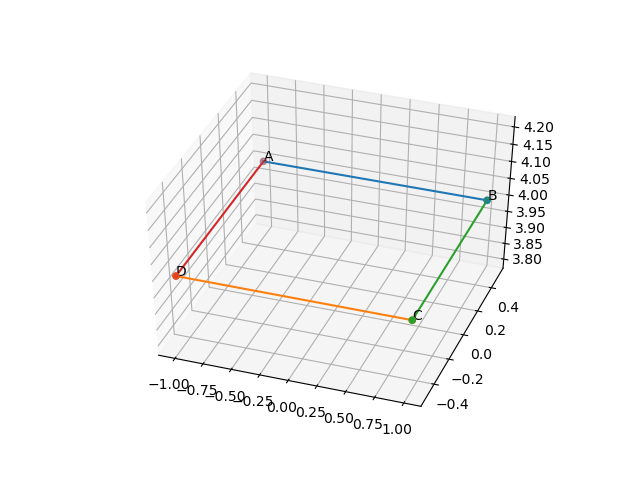
\includegraphics[width=\columnwidth]{chapters/12/10/4/12/figs/Figure_1.png}
   \caption{}
   \label{fig:chapters/12/10/4/12Rect_ABCD}
\end{figure}





\item Find the area of the triangle whose vertices are 
\begin{enumerate}
\item $(2, 3), (–1, 0), (2, – 4)$
\item $(–5, –1), (3, –5), (5, 2)$ 
\end{enumerate}
		\label{10/7/3/1}
\solution
		    See \tabref{eq:10/7/3/1/area}.
\begin{table}[H]
    \centering
    \caption{}
    \label{eq:10/7/3/1/area}
    \begin{tabular}{|c|c|c|c|}
        \hline
	     & $\vec{A}-\vec{B}$  & $\vec{A}-\vec{C}$  & $\frac{1}{2}\|\brak{\vec{A}-\vec{B}} \times \brak{\vec{A}-\vec{C}}\|$ \\
        \hline
         a)& $\myvec{ 3 \\3 }$ & $\myvec{ 0 \\ 7 }$ & $\frac{21}{2}$ \\
        \hline
	    b)& $\myvec{
 -8 \\
 4 
 }$
         &$\myvec{
 -10 \\
 -3 
 }$
  &  $32$   \\
        \hline
    \end{tabular}
\end{table}


\item Find the area of the triangle formed by joining the mid-points of the sides of the triangle whose vertices are $A(0, –1), B(2, 1)$  and  $C(0, 3)$. Find the ratio of this area to the area of the given triangle.
	\\
\solution
		Using 
	  \eqref{eq:section_formula},
the mid point coordinates are given by
	\begin{align}
		\vec{P} = \frac{1}{2}\vec(\vec{A}+\vec{B})  = \myvec{1\\0}\\
		\vec{Q} = \frac{1}{2}\vec(\vec{B}+\vec{C}) = \myvec{1\\2}\\
		\vec{R} = \frac{1}{2}\vec(\vec{A}+\vec{C}) = \myvec{0\\1}
	\end{align}
	\begin{align}
\because		\vec{P}-\vec{Q} =  \myvec{
 0 \\
 -2 
 },\,
		\vec{Q}-\vec{R} =   \myvec{
 1 \\
 1 
 }
 \\
		ar(PQR)=\frac{1}{2}{\norm{\vec(\vec{P}-\vec{Q})\times\vec(\vec{Q}-\vec{R})}}
		=1
	\end{align}
	Similarly, 
	\begin{align}
		\vec{A}-\vec{B} = \myvec{
 -2 \\
 -2 
 }
 ,\,
		\vec{A}-\vec{C} =  \myvec{
 0 \\
 -4 
 }
 \\
 \implies
		ar(ABC)=\frac{1}{2}{\norm{\vec(\vec{A}-\vec{B})\times\vec(\vec{A}-\vec{C})}}
=4
\\
		\implies \frac{ar\brak{PQR}}{ar\brak{ABC}} = \frac{1}{4}
	\end{align}
	See 
\figref{fig:10/7/3/3Fig}
\begin{figure}[H]
	\begin{center} 
	    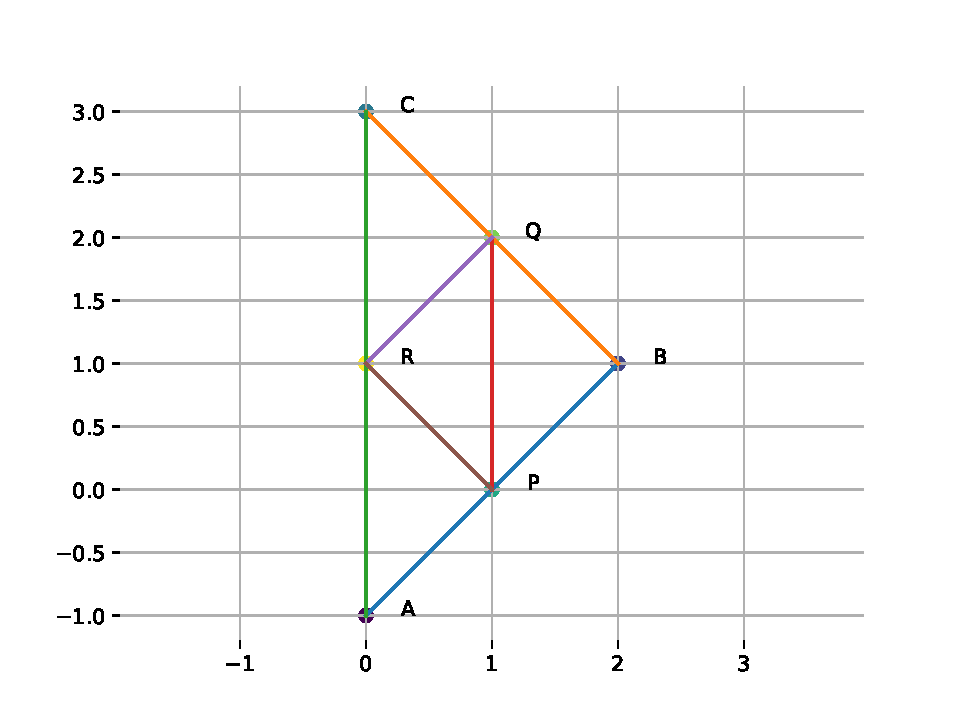
\includegraphics[width=0.75\columnwidth]{chapters/10/7/3/3/figs/fig.pdf}
	\end{center}
\caption{}
\label{fig:10/7/3/3Fig}
\end{figure}


\item Find the area of the quadrilateral whose vertices, taken in order, are $A(– 4, – 2), B(– 3, – 5), C(3, – 2)$  and $ D(2, 3)$.
	\\
\solution
		\iffalse
\documentclass[12pt]{article}
\usepackage{graphicx}
%\documentclass[journal,12pt,twocolumn]{IEEEtran}
\usepackage[none]{hyphenat}
\usepackage{graphicx}
\usepackage{listings}
\usepackage[english]{babel}
\usepackage{graphicx}
\usepackage{caption} 
\usepackage{hyperref}
\usepackage{booktabs}
\def\inputGnumericTable{}
\usepackage{color}                                            %%
    \usepackage{array}                                            %%
    \usepackage{longtable}                                        %%
    \usepackage{calc}                                             %%
    \usepackage{multirow}                                         %%
    \usepackage{hhline}                                           %%
    \usepackage{ifthen}
\usepackage{array}
\usepackage{amsmath}   % for having text in math mode
\usepackage{listings}
\lstset{
language=tex,
frame=single, 
breaklines=true
}
  
%Following 2 lines were added to remove the blank page at the beginning
\usepackage{atbegshi}% http://ctan.org/pkg/atbegshi
\AtBeginDocument{\AtBeginShipoutNext{\AtBeginShipoutDiscard}}
%
%New macro definitions
\newcommand{\mydet}[1]{\ensuremath{\begin{vmatrix}#1\end{vmatrix}}}
\providecommand{\brak}[1]{\ensuremath{\left(#1\right)}}
\providecommand{\norm}[1]{\left\lVert#1\right\rVert}
\newcommand{\solution}{\noindent \textbf{Solution: }}
\newcommand{\myvec}[1]{\ensuremath{\begin{pmatrix}#1\end{pmatrix}}}
\let\vec\mathbf
\begin{document}
\begin{center}
\title{\textbf{Coordinate Geometry}}
\date{\vspace{-5ex}} %Not to print date automatically
\maketitle
\end{center}
\setcounter{page}{1}
\section*{10$^{th}$ Maths - Chapter 7}
This is Problem-4 from Exercise 7.3
\begin{enumerate}
\item Find the area of quadrilateral whose vertices, taken in order, are $\myvec{-4 \\ -2}, \myvec{-3\\-5}, \myvec{3\\-2}$ and $\myvec{2\\3}$.\\
	\solution 
\fi
		The input parameters for this problem are available in Table \eqref{tab:10/7/3/4}.
\begin{table}[ht!]\centering
%%%%%%%%%%%%%%%%%%%%%%%%%%%%%%%%%%%%%%%%%%%%%%%%%%%%%%%%%%%%%%%%%%%%%%
%%                                                                  %%
%%  This is the header of a LaTeX2e file exported from Gnumeric.    %%
%%                                                                  %%
%%  This file can be compiled as it stands or included in another   %%
%%  LaTeX document. The table is based on the longtable package so  %%
%%  the longtable options (headers, footers...) can be set in the   %%
%%  preamble section below (see PRAMBLE).                           %%
%%                                                                  %%
%%  To include the file in another, the following two lines must be %%
%%  in the including file:                                          %%
%%        \def\inputGnumericTable{}                                 %%
%%  at the beginning of the file and:                               %%
%%        \input{name-of-this-file.tex}                             %%
%%  where the table is to be placed. Note also that the including   %%
%%  file must use the following packages for the table to be        %%
%%  rendered correctly:                                             %%
%%    \usepackage[latin1]{inputenc}                                 %%
%%    \usepackage{color}                                            %%
%%    \usepackage{array}                                            %%
%%    \usepackage{longtable}                                        %%
%%    \usepackage{calc}                                             %%
%%    \usepackage{multirow}                                         %%
%%    \usepackage{hhline}                                           %%
%%    \usepackage{ifthen}                                           %%
%%  optionally (for landscape tables embedded in another document): %%
%%    \usepackage{lscape}                                           %%
%%                                                                  %%
%%%%%%%%%%%%%%%%%%%%%%%%%%%%%%%%%%%%%%%%%%%%%%%%%%%%%%%%%%%%%%%%%%%%%%



%%  This section checks if we are begin input into another file or  %%
%%  the file will be compiled alone. First use a macro taken from   %%
%%  the TeXbook ex 7.7 (suggestion of Han-Wen Nienhuys).            %%
\def\ifundefined#1{\expandafter\ifx\csname#1\endcsname\relax}


%%  Check for the \def token for inputed files. If it is not        %%
%%  defined, the file will be processed as a standalone and the     %%
%%  preamble will be used.                                          %%
\ifundefined{inputGnumericTable}

%%  We must be able to close or not the document at the end.        %%
 \def\gnumericTableEnd{\end{document}}


%%%%%%%%%%%%%%%%%%%%%%%%%%%%%%%%%%%%%%%%%%%%%%%%%%%%%%%%%%%%%%%%%%%%%%
%%                                                                  %%
%%  This is the PREAMBLE. Change these values to get the right      %%
%%  paper size and other niceties.                                  %%
%%                                                                  %%
%%%%%%%%%%%%%%%%%%%%%%%%%%%%%%%%%%%%%%%%%%%%%%%%%%%%%%%%%%%%%%%%%%%%%%

 \documentclass[12pt%
     %,landscape%
                    ]{report}
       \usepackage[latin1]{inputenc}
       \usepackage{fullpage}
       \usepackage{color}
       \usepackage{array}
       \usepackage{longtable}
       \usepackage{calc}
       \usepackage{multirow}
       \usepackage{hhline}
       \usepackage{ifthen}

 \begin{document}


%%  End of the preamble for the standalone. The next section is for %%
%%  documents which are included into other LaTeX2e files.          %%
\else

%%  We are not a stand alone document. For a regular table, we will %%
%%  have no preamble and only define the closing to mean nothing.   %%
    \def\gnumericTableEnd{}

%%  If we want landscape mode in an embedded document, comment out  %%
%%  the line above and uncomment the two below. The table will      %%
%%  begin on a new page and run in landscape mode.                  %%
%       \def\gnumericTableEnd{\end{landscape}}
%       \begin{landscape}


%%  End  theoelse clause for this file being \input.              %%
\fi

%%%%%%%%%%%%%%%%%%%%%%%%%%%%%%%%%%%%%%%%%%%%%%%%%%%%%%%%%%%%%%%%%%%%%%
%%                                                                  %%
%%  The rest is the gnumeric table, except for the closing          %%
%%  statement. Changes below will alter the table's appearance.     %%
%%                                                                  %%
%%%%%%%%%%%%%%%%%%%%%%%%%%%%%%%%%%%%%%%%%%%%%%%%%%%%%%%%%%%%%%%%%%%%%%

\providecommand{\gnumericmathit}[1]{#1} 
%%  Uncomment the next line if you would like your numbers to be in %%
%%  italics if they are italizised in the gnumeric table.           %%
%\renewcommand{\gnumericmathit}[1]{\mathit{#1}}
\providecommand{\gnumericPB}[1]%
{\let\gnumericTemp=\\#1\let\\=\gnumericTemp\hspace{0pt}}
 \ifundefined{gnumericTableWidthDefined}
        \newlength{\gnumericTableWidth}
        \newlength{\gnumericTableWidthComplete}
        \newlength{\gnumericMultiRowLength}
        \global\def\gnumericTableWidthDefined{}
 \fi
%% The following setting protects this code from babel shorthands.  %%
 \ifthenelse{\isundefined{\languageshorthands}}{}{\languageshorthands{english}}
%%  The default table format retains the relative column widths of  %%
%%  gnumeric. They can easily be changed to c, r or l. In that case %%
%%  you may want to comment out the next line and uncomment the one %%
%%  thereafter                                                      %%
\providecommand\gnumbox{\makebox[0pt]}
%%\providecommand\gnumbox[1][]{\makebox}

%% to adjust positions in multirow situations                       %%
\setlength{\bigstrutjot}{\jot}
\setlength{\extrarowheight}{\doublerulesep}

%%  The \setlongtables command keeps column widths the same across  %%
%%  pages. Simply comment out next line for varying column widths.  %%
\setlongtables

\setlength\gnumericTableWidth{%
 53pt+%
 53pt+%
 82pt+%
 53pt+%
0pt}
\def\gumericNumCols{4}
\setlength\gnumericTableWidthComplete{\gnumericTableWidth+%
         \tabcolsep*\gumericNumCols*2+\arrayrulewidth*\gumericNumCols}
\ifthenelse{\lengthtest{\gnumericTableWidthComplete > \linewidth}}%
         {\def\gnumericScale{1*\ratio{\linewidth-%
                        \tabcolsep*\gumericNumCols*2-%
                        \arrayrulewidth*\gumericNumCols}%
{\gnumericTableWidth}}}%
{\def\gnumericScale{1}}

%%%%%%%%%%%%%%%%%%%%%%%%%%%%%%%%%%%%%%%%%%%%%%%%%%%%%%%%%%%%%%%%%%%%%%
%%                                                                  %%
%% The following are the widths of the various columns. We are      %%
%% defining them here because then they are easier to change.       %%
%% Depending on the cell formats we may use them more than once.    %%
%%                                                                  %%
%%%%%%%%%%%%%%%%%%%%%%%%%%%%%%%%%%%%%%%%%%%%%%%%%%%%%%%%%%%%%%%%%%%%%%

\ifthenelse{\isundefined{\gnumericColA}}{\newlength{\gnumericColA}}{}\settowidth{\gnumericColA}{\begin{tabular}{@{}p{53pt*\gnumericScale}@{}}x\end{tabular}}
\ifthenelse{\isundefined{\gnumericColB}}{\newlength{\gnumericColB}}{}\settowidth{\gnumericColB}{\begin{tabular}{@{}p{53pt*\gnumericScale}@{}}x\end{tabular}}
\ifthenelse{\isundefined{\gnumericColC}}{\newlength{\gnumericColC}}{}\settowidth{\gnumericColC}{\begin{tabular}{@{}p{82pt*\gnumericScale}@{}}x\end{tabular}}
\ifthenelse{\isundefined{\gnumericColD}}{\newlength{\gnumericColD}}{}\settowidth{\gnumericColD}{\begin{tabular}{@{}p{53pt*\gnumericScale}@{}}x\end{tabular}}

\begin{center}
\begin{tabular}[c]{%
 b{\gnumericColA}%
 b{\gnumericColB}%
 b{\gnumericColC}%
 b{\gnumericColD}%
 }

%%%%%%%%%%%%%%%%%%%%%%%%%%%%%%%%%%%%%%%%%%%%%%%%%%%%%%%%%%%%%%%%%%%%%%
%%  The longtable options. (Caption, headers... see Goosens, p.124) %%
% \caption{The Table Caption.}             \\ %
% \hline % Across the top of the table.
%%  The rest of these options are table rows which are placed on    %%
%%  the first, last or every page. Use \multicolumn if you want.    %%

%%  Header for the first page.                                      %%
% \multicolumn{4}{c}{The First Header} \\ \hline 
% \multicolumn{1}{c}{colTag} %Column 1
% &\multicolumn{1}{c}{colTag} %Column 2
% &\multicolumn{1}{c}{colTag} %Column 3
% &\multicolumn{1}{c}{colTag} \\ \hline %Last column
% \endfirsthead

%%  The running header definition.                                  %%
% \hline
% \multicolumn{4}{l}{\ldots\small\slshape continued} \\ \hline
% \multicolumn{1}{c}{colTag} %Column 1
% &\multicolumn{1}{c}{colTag} %Column 2
% &\multicolumn{1}{c}{colTag} %Column 3
% &\multicolumn{1}{c}{colTag} \\ \hline %Last column
% \endhead

%%  The running footer definition.                                  %%
% \hline
% \multicolumn{4}{r}{\small\slshape continued\ldots} \\
% \endfoot

%%  The ending footer definition.                                   %%
% \multicolumn{4}{c}{That's all folks} \\ \hline 
% \endlastfoot
%%%%%%%%%%%%%%%%%%%%%%%%%%%%%%%%%%%%%%%%%%%%%%%%%%%%%%%%%%%%%%%%%%%%%%

\hhline{|-|-|-~}
  \multicolumn{1}{|p{\gnumericColA}|}%
 {\gnumericPB{\centering}\gnumbox{\textbf{Symbol}}}
 &\multicolumn{1}{p{\gnumericColB}|}%
 {\gnumericPB{\centering}\gnumbox{\textbf{Value}}}
 &\multicolumn{1}{p{\gnumericColC}|}%
 {\gnumericPB{\centering}\gnumbox{\textbf{Description}}}
 &
\\
\hhline{|---|~}
  \multicolumn{1}{|p{\gnumericColA}|}%
 {\gnumericPB{\centering}\gnumbox{$\vec{A}$}}
 &\multicolumn{1}{p{\gnumericColB}|}%
 {\gnumericPB{\centering}\gnumbox{$\myvec{-4\\-2}$}}
 &\multicolumn{1}{p{\gnumericColC}|}%
 {\gnumericPB{\centering}\gnumbox{First point}}
 &
\\
\hhline{|---|~}
  \multicolumn{1}{|p{\gnumericColA}|}%
 {\gnumericPB{\centering}\gnumbox{$\vec{B}$}}
 &\multicolumn{1}{p{\gnumericColB}|}%
 {\gnumericPB{\centering}\gnumbox{$\myvec{-3\\-5}$}}
 &\multicolumn{1}{p{\gnumericColC}|}%
 {\gnumericPB{\centering}\gnumbox{Second point}}
 &
\\
\hhline{|---|~}
  \multicolumn{1}{|p{\gnumericColA}|}%
 {\gnumericPB{\centering}\gnumbox{$\vec{C}$}}
 &\multicolumn{1}{p{\gnumericColB}|}%
 {\gnumericPB{\centering}\gnumbox{$\myvec{3\\-2}$}}
 &\multicolumn{1}{p{\gnumericColC}|}%
 {\gnumericPB{\centering}\gnumbox{Third point}}
 &
\\

\hhline{|---|~}
  \multicolumn{1}{|p{\gnumericColA}|}%
 {\gnumericPB{\centering}\gnumbox{$\vec{D}$}}
 &\multicolumn{1}{p{\gnumericColB}|}%
 {\gnumericPB{\centering}\gnumbox{$\myvec{2\\3}$}}
 &\multicolumn{1}{p{\gnumericColC}|}%
 {\gnumericPB{\centering}\gnumbox{Fourth point}}
 &
\\
\hhline{|-|-|-|~}
\end{tabular}
 \end{center}

\ifthenelse{\isundefined{\languageshorthands}}{}{\languageshorthands{\languagename}}
%\gnumericTableEndf

\caption{}
\label{tab:10/7/3/4}	
\end{table}
By joining $\vec{B}$ to $\vec{D}$, two triangles $\vec{A}\vec{B}\vec{D}$ and $\vec{B}\vec{C}\vec{D}$ are obtained.
Since
\begin{align}
	\vec{A}- \vec{B} &= \myvec{-4\\-2\\}-\myvec{-3\\-5\\}=\myvec{-1\\3\\}\label{eq:chapters/10/7/3/4/2}\\
	  \vec{A}- \vec{D} &= \myvec{-4\\-2\\}-\myvec{2\\3\\}=\myvec{-6\\-5\\}\label{eq:chapters/10/7/3/4/3}
  \end{align}
  \begin{align}
	  ar(ABD)&=\frac{1}{2} \norm{\brak{\vec{A}-\vec{B}}  \times 
   \brak{\vec{A}- \vec{D}}} \label{eq:chapters/10/7/3/4/1} 
   \\
	  &=	\frac{1}{2}\mydet{-1 & 3\\-6 & -5}  
	=	\frac{23}{2}
\end{align}
upon substituting the values of \eqref{eq:chapters/10/7/3/4/2} and \eqref{eq:chapters/10/7/3/4/3} in \eqref{eq:chapters/10/7/3/4/1}.
Similarly,
\begin{align}
	\vec{B}- \vec{C} &= \myvec{-3\\-5\\}-\myvec{3\\-2\\}=\myvec{-6\\-5\\}\label{eq:chapters/10/7/3/4/6} \\
	  \vec{B}- \vec{D} &= \myvec{-3\\-5\\}-\myvec{2\\3\\}=\myvec{-3\\-8\\}\label{eq:chapters/10/7/3/4/7} 
  \end{align}
  yielding
  \begin{align}
	  ar(BCD)&=\frac{1}{2} \norm{\brak{\vec{B}-\vec{C}}  \times 
   \brak{\vec{B}- \vec{D}}} \label{eq:chapters/10/7/3/4/5}
   \\
	  &=	\frac{1}{2}\mydet{-6 & -3\\-5 & -8}  
	=	\frac{33}{2}
\end{align}
	upon 	substituting the values of \eqref{eq:chapters/10/7/3/4/6} and \eqref{eq:chapters/10/7/3/4/7} in \eqref{eq:chapters/10/7/3/4/5}
		Thus, 
\begin{align}
	ar(ABCD)&=  ar(ABD) +  ar(BCD)
	= 28
\end{align}
See Fig. 
\ref{fig:chapters/10/7/3/4/Fig1}
\begin{figure}[!h]
 \begin{center}
  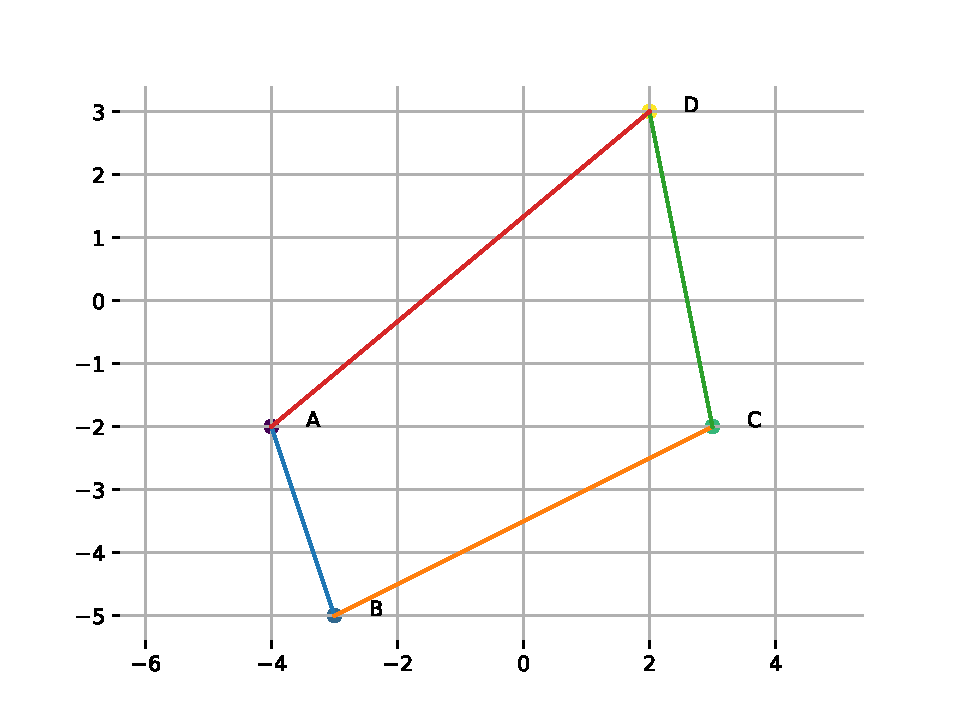
\includegraphics[width=\columnwidth]{chapters/10/7/3/4/figs/fig.pdf}
 \end{center}
\caption{}
\label{fig:chapters/10/7/3/4/Fig1}
\end{figure}


\item Verify that a median of a triangle divides it into two triangles of equal areas for $\triangle ABC$ whose vertices are $\vec{A}(4, -6), \vec{B}(3, 2), \text{ and } \vec{C}(5, 2)$. 
		\label{10/7/3/5}
		\\
\solution
		\begin{align}
\vec{D}=\frac{\vec{B}+\vec{C}}{2}
=\myvec{4\\ 0},
\\
	\vec{A}- \vec{B} =\myvec{1\\ -4},\,
	  \vec{A}- \vec{D} =\myvec{0\\ -6}
	  \\
	  \implies
  ar(ABD)=\frac{1}{2} \norm{\brak{\vec{A}-\vec{B}}  \times 
   \brak{\vec{A}- \vec{D}}} 
	       =3	
	       \\
	\vec{A}- \vec{C} =\myvec{-1\\ -8},\,
	  \vec{A}- \vec{D} =\myvec{0\\ -6}
	  \\
	  \implies
  ar(ACD)=\frac{1}{2} \norm{\brak{\vec{A}-\vec{C}}  \times 
   \brak{\vec{A}- \vec{D}}} 
   \\
	= 3 =
ar(ABD)
\end{align}
See  
\figref{fig:10/7/3/5/}.
\begin{figure}[H]
\centering
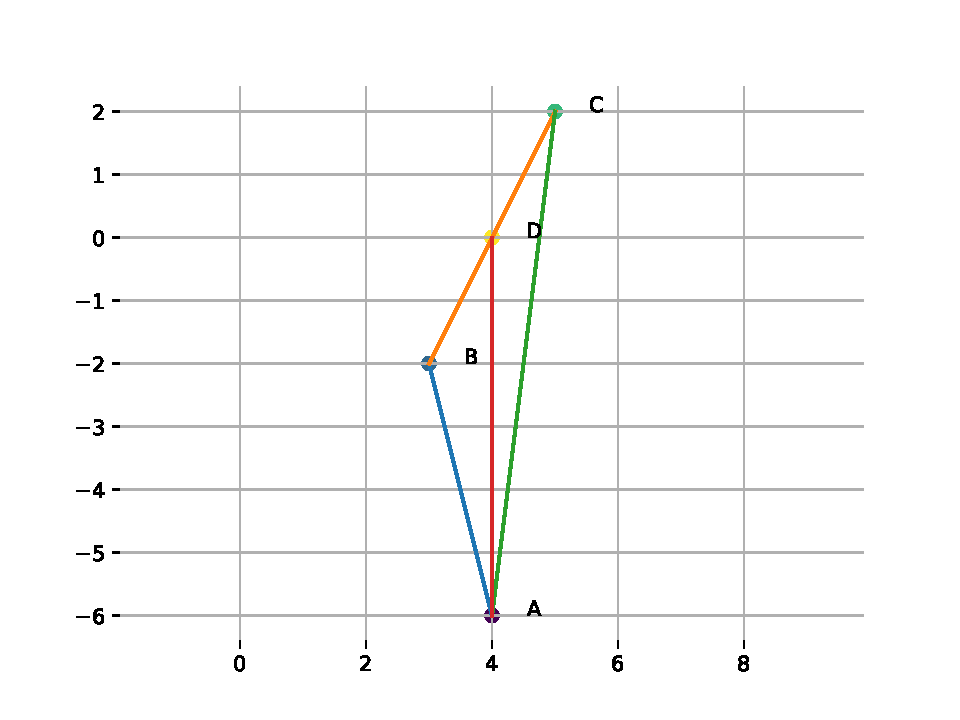
\includegraphics[width=0.75\columnwidth]{chapters/10/7/3/5/figs/fig.pdf}
\caption{}
\label{fig:10/7/3/5/}
\end{figure} 

\item The two adjacent sides of a parallelogram are 
$\vec{a}= 2\hat{i}-4\hat{j}+5\hat{k}$  and  $\vec{b} =\hat{i}-2\hat{j}-3\hat{k}$.
Find the unit vector parallel to its diagonal. Also, find its area.\\
	\solution
		\iffalse
\documentclass[journal,12pt,twocolumn]{IEEEtran}
\usepackage{setspace}
\usepackage{gensymb}
\usepackage{xcolor}
\usepackage{caption}
\singlespacing
\usepackage{siunitx}
\usepackage[cmex10]{amsmath}
\usepackage{mathtools}
\usepackage{hyperref}
\usepackage{amsthm}
\usepackage{mathrsfs}
\usepackage{txfonts}
\usepackage{stfloats}
\usepackage{cite}
\usepackage{cases}
\usepackage{subfig}
\usepackage{longtable}
\usepackage{multirow}
\usepackage{enumitem}
\usepackage{bm}
\usepackage{mathtools}
\usepackage{listings}
\usepackage{tikz}
\usetikzlibrary{shapes,arrows,positioning}
\usepackage{circuitikz}
\renewcommand{\vec}[1]{\boldsymbol{\mathbf{#1}}}
\DeclareMathOperator*{\Res}{Res}
\renewcommand\thesection{\arabic{section}}
\renewcommand\thesubsection{\thesection.\arabic{subsection}}
\renewcommand\thesubsubsection{\thesubsection.\arabic{subsubsection}}

\renewcommand\thesectiondis{\arabic{section}}
\renewcommand\thesubsectiondis{\thesectiondis.\arabic{subsection}}
\renewcommand\thesubsubsectiondis{\thesubsectiondis.\arabic{subsubsection}}
\hyphenation{op-tical net-works semi-conduc-tor}

\lstset{
language=Python,
frame=single, 
breaklines=true,
columns=fullflexible
}
\begin{document}
\theoremstyle{definition}
\newtheorem{theorem}{Theorem}[section]
\newtheorem{problem}{Problem}
\newtheorem{proposition}{Proposition}[section]
\newtheorem{lemma}{Lemma}[section]
\newtheorem{corollary}[theorem]{Corollary}
\newtheorem{example}{Example}[section]
\newtheorem{definition}{Definition}[section]
\newcommand{\BEQA}{\begin{eqnarray}}
        \newcommand{\EEQA}{\end{eqnarray}}
\newcommand{\define}{\stackrel{\triangle}{=}}
\newcommand{\myvec}[1]{\ensuremath{\begin{pmatrix}#1\end{pmatrix}}}
\newcommand{\mydet}[1]{\ensuremath{\begin{vmatrix}#1\end{vmatrix}}}
\bibliographystyle{IEEEtran}
\providecommand{\nCr}[2]{\,^{#1}C_{#2}} % nCr
\providecommand{\nPr}[2]{\,^{#1}P_{#2}} % nPr
\providecommand{\mbf}{\mathbf}
\providecommand{\pr}[1]{\ensuremath{\Pr\left(#1\right)}}
\providecommand{\qfunc}[1]{\ensuremath{Q\left(#1\right)}}
\providecommand{\sbrak}[1]{\ensuremath{{}\left[#1\right]}}
\providecommand{\lsbrak}[1]{\ensuremath{{}\left[#1\right.}}
\providecommand{\rsbrak}[1]{\ensuremath{{}\left.#1\right]}}
\providecommand{\brak}[1]{\ensuremath{\left(#1\right)}}
\providecommand{\lbrak}[1]{\ensuremath{\left(#1\right.}}
\providecommand{\rbrak}[1]{\ensuremath{\left.#1\right)}}
\providecommand{\cbrak}[1]{\ensuremath{\left\{#1\right\}}}
\providecommand{\lcbrak}[1]{\ensuremath{\left\{#1\right.}}
\providecommand{\rcbrak}[1]{\ensuremath{\left.#1\right\}}}
\theoremstyle{remark}
\newtheorem{rem}{Remark}
\newcommand{\sgn}{\mathop{\mathrm{sgn}}}
\newcommand{\rect}{\mathop{\mathrm{rect}}}
\newcommand{\sinc}{\mathop{\mathrm{sinc}}}
\providecommand{\abs}[1]{\left\vert#1\right\vert}
\providecommand{\res}[1]{\Res\displaylimits_{#1}}
\providecommand{\norm}[1]{\lVert#1\rVert}
\providecommand{\mtx}[1]{\mathbf{#1}}
\providecommand{\mean}[1]{E\left[ #1 \right]}
\providecommand{\fourier}{\overset{\mathcal{F}}{ \rightleftharpoons}}
\providecommand{\ztrans}{\overset{\mathcal{Z}}{ \rightleftharpoons}}
\providecommand{\system}[1]{\overset{\mathcal{#1}}{ \longleftrightarrow}}
\newcommand{\solution}{\noindent \textbf{Solution: }}
\providecommand{\dec}[2]{\ensuremath{\overset{#1}{\underset{#2}{\gtrless}}}}
\let\StandardTheFigure\thefigure
\def\putbox#1#2#3{\makebox[0in][l]{\makebox[#1][l]{}\raisebox{\baselineskip}[0in][0in]{\raisebox{#2}[0in][0in]{#3}}}}
\def\rightbox#1{\makebox[0in][r]{#1}}
\def\centbox#1{\makebox[0in]{#1}}
\def\topbox#1{\raisebox{-\baselineskip}[0in][0in]{#1}}
\def\midbox#1{\raisebox{-0.5\baselineskip}[0in][0in]{#1}}

\vspace{3cm}
\title{12.10.5.10}
\author{Lokesh Surana}
\maketitle
\section*{Class 12, Chapter 10, Exercise 5.10}

Q.10. The two adjacent sides of a parallelogram are  ${2}\hat{i} -  {4}\hat{j} + {5}\hat{k}$ and ${1}\hat{i} -  {2}\hat{j} - {3}\hat{k}$.
Find the unit vector parallel to its diagonal. Also, find its area.

\solution 
\fi
Let the sides of the parallelogram be 
\begin{align}
\vec{a} = \myvec{2\\-4\\5}, \, \vec{b} = \myvec{1\\-2\\-3}.
\end{align}
The diagonals of the parallelogram are given by
\begin{align}
	\vec{D}_1 &= \vec{a} + \vec{b} = \myvec{3 \\-6\\2} \\
	\vec{D}_2 &= \vec{a} - \vec{b} = \myvec{1 \\-2\\8}
\end{align}
The unit vectors parallel to the diagonals are then given by
\begin{align}
	\hat{\vec{D}_1} &= \frac{\vec{D}_1}{\norm{\vec{D}_1}}  = \myvec{\frac{3}{\sqrt{45}}\\-\frac{6}{\sqrt{45}}\\\frac{2}{\sqrt{45}}} \\
    \hat{\vec{D}_2} &= \frac{\vec{D}_2}{\norm{\vec{D}_2}}  = \myvec{\frac{1}{\sqrt{69}}\\-\frac{2}{\sqrt{69}}\\\frac{8}{\sqrt{69}}}
\end{align}
%
Since
\begin{align}
    \vec{a}\times\vec{b}=\myvec{22 \\-11\\0},
\end{align}
he area of the parallelogram is given by
\begin{align}
    \norm{\vec{a}\times\vec{b}}  = \sqrt{605}
\end{align}


\item The vertices of a $\triangle ABC$ are $\vec{A}(4,6), \vec{B}(1,5)$ and  $\vec{C}(7,2)$. A line is drawn to intersect sides $AB$ and $AC$ at $\vec{D}$ and $\vec{E}$ respectively, such that $\frac{AD}{AB} = \frac{AE}{AC} = \frac{1}{4}$. Calculate the area of $\triangle ADE$ and compare it with the area of the $\triangle ABC$.
\\
\solution
	See  
\figref{fig:chapters/10/7/4/6Fig1}.
\begin{figure}[H]
 \begin{center}
 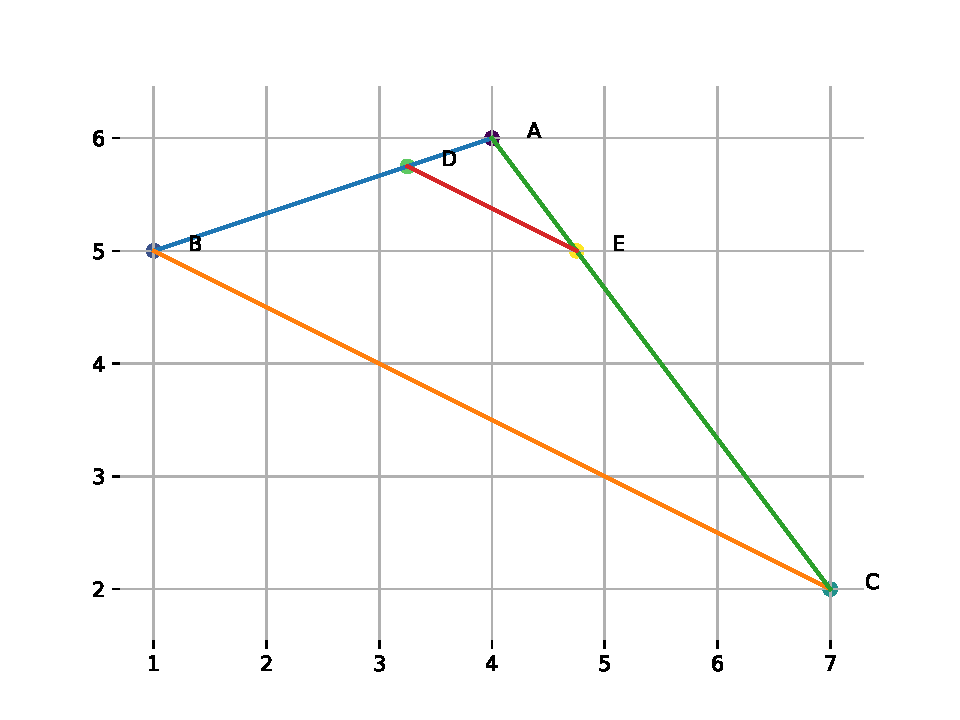
\includegraphics[width=0.75\columnwidth]{chapters/10/7/4/6/figs/fig.pdf}
 \end{center}
\caption{}
\label{fig:chapters/10/7/4/6Fig1}
\end{figure}
	Using section formula
	  \eqref{eq:section_formula},
\begin{align}
\vec{D} =\frac{3\vec{A}+\vec{B}}{4}
	=\frac{1}{4}\myvec{13\\ 23}
	\\
\vec{E} =\frac{3\vec{A}+\vec{C}}{4}
	=\frac{1}{4}\myvec{19\\ 20}
	\\
	\vec{A}- \vec{D} 
	=\frac{1}{4}\myvec{3\\ 1},\,
	  \vec{A}- \vec{E}  
	=\frac{1}{4}\myvec{-3\\ 1}
	\\
	\vec{A}- \vec{B} =\myvec{3\\1},
	  \vec{B}-\vec{C} =\myvec{-6\\3}
\end{align}
yielding
\begin{align}
ar(ABD) =\frac{1}{2} \norm{\brak{\vec{A}-\vec{D}}  \times 
   \brak{\vec{A}- \vec{E}}} 
	=	\frac{15}{32}
	\\
	  ar(ABC) =\frac{1}{2} \norm{\brak{\vec{A}-\vec{B}}  \times 
   \brak{\vec{B}- \vec{C}}} 
	=	\frac{15}{2}
	\\
	\implies \frac{ar\brak{ADE}}{ar\brak{ABC}}=\frac{1}{16}
\end{align}

    \item Draw a quadrilateral in the Cartesian plane, whose vertices are 
    \begin{align}
        \vec{A} = \myvec{-4\\5},\, \vec{B} = \myvec{0\\7},\, 
        \vec{C} = \myvec{5\\-5},\, \vec{D} = \myvec{-4\\-2}.
    \end{align}
    Also, find its area.
\label{chapters/11/10/1/1}
   \\ 
    \solution 
See \figref{fig:11/10/1/1quad}.
    From 
        \eqref{eq:11/10/1/1area-diag},
    \begin{align}
ar\brak{ABCD}
	       = \frac{121}{2}
        \label{eq:11/10/1/1ans}
    \end{align}
    \begin{figure}[H]
        \centering
        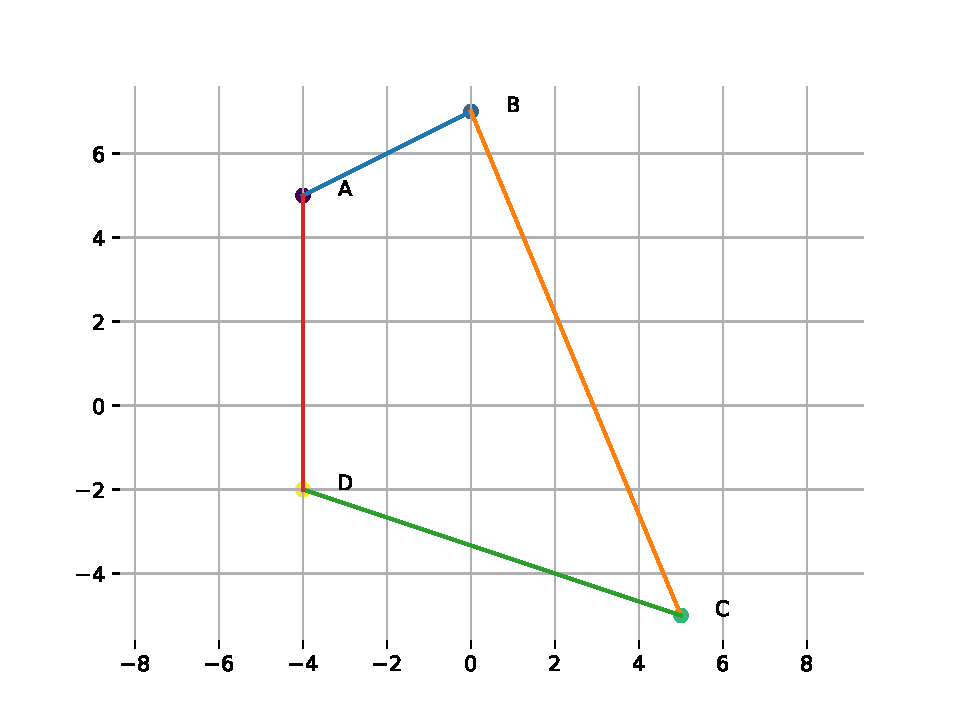
\includegraphics[width=0.75\columnwidth]{chapters/11/10/1/1/figs/fig.pdf}
        \caption{Plot of quadrilateral $ABCD$}
        \label{fig:11/10/1/1quad}
    \end{figure}

\item Find the area of region bounded by the triangle whose
	vertices are $(1, 0), (2, 2)$ and $(3, 1)$. 
\item Find the area of region bounded by the triangle whose vertices
	are $(– 1, 0), (1, 3)$  and  $(3, 2)$. 
\item Find the area of the $\triangle ABC$, coordinates of whose vertices are $\vec{A}(2, 0), \vec{B}(4, 5)$ and $\vec{C}(6, 3)$.
\item The area of a triangle with vertices $\vec{A}(3, 0), \vec{B}(7, 0)$ and  $\vec{C}(8, 4)$ is
\begin{enumerate}
\item 14
\item 28
\item 8
\item 6
\end{enumerate}
\item Find the area of the triangle whose vertices are $(-8,4),(-6,6)$ and $(-3,9)$.
\item If $\vec{D}\brak{\frac{-1}{2},\frac{5}{2}},\vec{E}(7,3)$ and $\vec{F}\brak{\frac{7}{2},\frac{7}{2}}$ are the midpoints of sides of $\triangle ABC$, find the area of the $\triangle ABC$.
\item Find the sine of the angle between the vectors $\vec{a}=3\hat{i}+\hat{j}+2\hat{k}$ $\text{ and }$ $\vec{b}=2\hat{i}-2\hat{j}+4\hat{k}$.
\item Using vectors, find the area of $\triangle{ABC}$ with vertices A(1,2,3), B(2,-1,4) and C(4,5,-1).
\item Find the area of the parallelogram whose diagonals are $2\hat{i}-\hat{j}+\hat{k}$ and $\hat{i}+3\hat{j}-\hat{k}$.

\item The vector from origin to the points A and B are $\vec{a}$ = $2\hat{i}-3\hat{j}+2\hat{k}$ and  $\vec{b}$ = $2\hat{i}+3\hat{j}+\hat{k}$, respectively, then the area of $\triangle {OAB}$ is
	\begin{enumerate}
\item 340 
\item $\sqrt{25}$
\item $\sqrt{229}$
\item $\frac{1}{2}\sqrt{229}$
\end{enumerate}
\item If $\vec{a} = \hat{i}+\hat{j}+\hat{k}$ and $\vec{b} = \hat{j}-\hat{k}$, find a vector $\vec{c}$ such that $\vec{a}\times\vec{c} = \vec{b}$ and $\vec{a}\cdot \vec{c}$ = 3.
%
\item The area of the quadrilateral ABCD, where A$(0,4,1)$, B$(2,3,-1)$, C$(4,5,0)$ and D$(2,6,2)$, is equal to 
\begin{enumerate}
	\item 9 sq. units
	\item 18 sq. units 
	\item 27 sq. units 
	\item 81 sq. units
\end{enumerate}
\item Find the area of region bounded by the triangle whose vertices are $(-1, 1), (0, 5)$ and $(3, 2)$.
\item The value of $\hat{i}\cdot(\hat{j}\times\hat{k})+\hat{j}\cdot(\hat{i}\times\hat{k})+\hat{k}\cdot(\hat{i}\times\hat{j})$ is
\begin{enumerate}
\item 0
\item -1
\item 1
\item 3
\end{enumerate}
\item The value of $\hat{i}\cdot (\hat{j}\times\hat{k})+\hat{j}\cdot (\hat{i}\times\hat{k})+\hat{k}\cdot (\hat{i}\times\hat{j})$ is
\begin{enumerate}
\item 0
\item -1
\item 1
\item 3
\end{enumerate}
\end{enumerate}


\subsection{CBSE}
\begin{enumerate}[label=\thesubsection.\arabic*,ref=\thesubsection.\theenumi]
\item The area of a triangle formed by vertices $\vec{O}$, $\vec{A}$ and $\vec{B}$, where $\overrightarrow{OA}= \hat{i}+2 \hat{j}+3\hat{k}$ and $\overrightarrow{OB}= -3\hat{i} - 2\hat{j} + \hat{k}$ is
\hfill (12, 2020)
    \item The area of the triangle formed by the line $ \frac{x}{a} + \frac{y}{b} = 1 $ with the coordinate axes is 
    \hfill (10, 2023)
    \item  Find the area of the triangle whose vertices are $(-1, 1)$, $(0, 5)$, and $(3, 2)$.
    \hfill (12, 2023)
    \item If $\overrightarrow{a}$ and $\overrightarrow{b}$ are two vectors such that
    \begin{align}
        \overrightarrow{a} = \hat{i} - \hat{j} + \hat{k}
    \end{align}
    and
    \begin{align}
        \overrightarrow{b} = 2\hat{i} - \hat{j} - 3\hat{k},
    \end{align}
    then find the vector $\overrightarrow{c}$, given that
    \begin{align}
        \overrightarrow{a} \times \overrightarrow{c} = \overrightarrow{b}
    \end{align}
    and
    \begin{align}
        \overrightarrow{a} \cdot \overrightarrow{c} = 4.
    \end{align}
    \hfill (12, 2023)
    \item If
    \begin{align}
        \overrightarrow{a} = 2\hat{i} + \hat{j} + 3\hat{k},
    \end{align}
    \begin{align}
        \overrightarrow{b} = -\hat{i} + 2\hat{j} + \hat{k},
    \end{align}
    and
    \begin{align}
        \overrightarrow{c} = 3\hat{i} + \hat{j} + 2\hat{k},
    \end{align}
    then find $\overrightarrow{a} \cdot (\overrightarrow{b} \times \overrightarrow{c})$.
    \hfill (12, 2023)
    \item Using vectors, find the area of the triangle with vertices $\vec{A}(-1, 0, -2)$, $\vec{B}(0, 2, 1)$, and $\vec{C}(-1, 4, 1)$.
    \hfill (12, 2023)

    \item Find the area of the triangle with vertices $(2, 0)$, $(4, 5)$, and $(1, 4)$.
    \hfill (12, 2023)
    \item Find the area of the quadrilateral $ABCD$ whose vertices are $\vec{A}(-4, -3)$, $\vec{B}(3, -1)$, $\vec{C}(0, 5)$, and $\vec{D}(-4, 2)$.
    \hfill (10, 2022)
	\item Find $|\overrightarrow{a} \times \overrightarrow{b}|$, if $\overrightarrow{a} = 2\hat{i} + \hat{j} + 3\hat{k}$ and $\overrightarrow{b} = 3\hat{i} + 5\hat{j} - 2\hat{k}$. \hfill (12, 2019)
	\item Find the area of the triangular region whose sides have the equations $y = 2x + 1$, $y = 3x + 1$, and $x = 4$. \hfill (12, 2019)
	
	\item Find the area of the triangle whose vertices are $(1, 0)$, $(2, 2)$, and $(3, 1)$. \hfill (12, 2019)
	\item Find the area of the triangle whose vertices are $(-1, 1)$, $(0, 5)$, and $(3, 2)$. \hfill (12, 2019)
\item Find the area of a triangle whose vertices are $(1, -1)$, $(-4, 6)$, and $(-3, -5)$. \hfill (10, 2019)
\item Find the area of the triangle formed by joining the midpoints of the sides of the triangle $ABC$, whose vertices are $A(0, -1)$, $B(2, 1)$, and $C(0, 3)$. \hfill (10, 2019)
    \item Given vertices $\vec{A}(-5,7)$, $\vec{B}(-4,-5)$, $\vec{C}(-1,-6)$, and $\vec{D}(4,5)$ of a quadrilateral. Find the area of quadrilateral $\vec{ABCD}$. \hfill (10, 2018)
\item If $\theta$ is the angle between the two vectors $\hat{i} - 2\hat{j} + 3\hat{k}$ and $3\hat{i} - 2\hat{j} + \hat{k}$, find $\sin \theta$. \hfill (12, 2018)
\item For any two vectors $\overrightarrow{a}$ and $\overrightarrow{b}$, prove that
    \begin{align*}
    \brak{{\overrightarrow{a} \times \overrightarrow{b}}}^{2} = {\overrightarrow{a}^{2}}~~{\overrightarrow{b}^{2}} - \brak{{\overrightarrow{a} \cdot \overrightarrow{b}}}^{2} 
    \end{align*}

\hfill (12, 2018) 
\item Find the volume of a cuboid whose edges are given by $-3\hat{i}+7\hat{j}+5\hat{k}$,$-5\hat{i}+7\hat{j}-3\hat{k}$ and $7\hat{i}-5\hat{j}-3\hat{k}$.

\hfill (12, 2018) 
\item Find $\abs{\overrightarrow{a} \times \overrightarrow{b}}$, if $\overrightarrow{a}=2\hat{i}+\hat{j}+3\hat{k}$ and $\overrightarrow{b}=3\hat{i}+5\hat{j}-2\hat{k}$.
\hfill (12, 2018) 
    \item Show that the points $\vec{A} = 2\hat{i} - \hat{j} + \hat{k}$, $\vec{B} = \hat{i} - 3\hat{j} - 5\hat{k}$, and $\vec{C} = 3\hat{i} - 4\hat{j} - 4\hat{k}$ respectively, are the vertices of a right-angled triangle. Hence, find the area of the triangle. \hfill (12, 2017)
    \item The vertices of $\triangle ABC$ are $A \myvec{4, 6}$, $B \myvec{1, 5}$, and $C \myvec{7, 2}$. A line-segment $DE$ is drawn to intersect the sides $AB$ and $AC$ at $D$ and $E$ respectively such that $\frac{AD}{AB} = \frac{AE}{AC} = \frac{1}{3}$. Calculate the area of $\triangle ADE$ and compare it with the area of $\triangle ABC$. \hfill (10, 2016)
\item Find $\lambda$ and $\mu$ if
      \begin{align*}
          \myvec{\hat{i} + 3\hat{j} + 9\hat{k}} \times \myvec{3\hat{i} - \lambda \hat{j} + \mu \hat{k}} = \overrightarrow{0}.
      \end{align*}
      \hfill (12, 2016)
\item The two adjacent sides of a parallelogram are $2\hat{i}-4\hat{j}-5\hat{k}$ and $2\hat{i}+2\hat{j}+3\hat{k}$. Find the two unit vectors parallel to its diagonals. Using the diagonal vectors, find the area of the parallelogram. \hfill (12, 2016)
\item Find the values of $k$ so that the area of the triangle with vertices $\begin{bmatrix}1, -1\end{bmatrix}$, $\begin{bmatrix}-4, 2k\end{bmatrix}$, and $\begin{bmatrix}-k, -5\end{bmatrix}$ is $24$ sq. units. \hfill (10, 2015)
\item The area of a triangle whose vertices are $\brak{5,0}$, $\brak{8,0}$ and $\brak{8,4}$ $\brak{\text{in sq. units}}$ is
\hfill (10, 2012)
\item For what value of $k$, $\brak{ k > 0}$, s the area of the triangle with vertices $\brak{-2,5}$, $\brak{k,-4}$, and $\brak{2k+1,10}$ equal to $52$ sq. units? 
\hfill (10, 2012)

\item If the vertices of a triangle are $\brak{1,-3}$, $\brak{4,p}$ and $\brak{-9,7}$ and its area is $15$ sq. units, find the value$\brak{\text{s}}$ of $p$. 
\hfill (10, 2012)

\item Find the area of quadrilateral $ABCD$ whose vertices are $A\brak{-3,-1}$, $B\brak{-2,-4}$, $C\brak{4,-1}$ and $D\brak{3,4}$.
\hfill (10, 2012)
\item Find the area of the quadrilateral $ABCD$, whose vertices are $A(-3, -1)$, $B(-2, -4)$, $C(4, -1)$, and $D(3, 4)$.
\hfill (10, 2011)
\item Using integration, find the area of triangle ABC, whose vertices are A$\brak{2, 5}$, B$\brak{4, 7}$ and C$\brak{6, 2}$.
\hfill (12, 2018)
\item Using integration, find the area of the triangle whose vertices are $\brak{2,3},\brak{3,5}$ and $\brak{4,4}$
\hfill (12, 2018)
\item The area of a triangle formed by vertices $\vec{O}$, $\vec{A}$ and $\vec{B}$, where $\overrightarrow{OA}= \hat{i}+2 \hat{j}+3\hat{k}$ and $\overrightarrow{OB}= -3\hat{i} - 2\hat{j} + \hat{k}$ is
\hfill (12, 2020)
\item Find the value of $k$ so that the area of triangle $ABC$ with $A\brak{k + 1, 1}$, $B\brak{4, -3}$ and $C\brak{7, -k}$ is $6$ square units.
\hfill (10, 2019)
\item Using integration, find the area of triangle ABC, whose vertices are A$\brak{2, 5}$, B$\brak{4, 7}$ and C$\brak{6, 2}$.
\hfill (12, 2018)
\item Using integration, find the area of the triangle whose vertices are $\brak{2,3},\brak{3,5}$ and $\brak{4,4}$
\hfill (12, 2018)

\end{enumerate}

\subsection{Miscellaneous}
\begin{enumerate}[label=\thesubsection.\arabic*,ref=\thesubsection.\theenumi]
\item The two opposite vertices of a square are $(–1, 2)$  and $ (3, 2)$. Find the coordinates of the other two vertices.
\\
\solution
	\iffalse
\documentclass[12pt]{article}
\usepackage{graphicx}
\usepackage{amsmath}
\usepackage{mathtools}
\usepackage{gensymb}

\newcommand{\mydet}[1]{\ensuremath{\begin{vmatrix}#1\end{vmatrix}}}
\providecommand{\brak}[1]{\ensuremath{\left(#1\right)}}
\providecommand{\norm}[1]{\left\lVert#1\right\rVert}
\newcommand{\solution}{\noindent \textbf{Solution: }}
\newcommand{\myvec}[1]{\ensuremath{\begin{pmatrix}#1\end{pmatrix}}}
\let\vec\mathbf

\begin{document}
\begin{center}
\textbf\large{CHAPTER-7 \\ COORDINATE GEOMETRY}

\end{center}
\section*{Excercise 7.4}

Q4.The two opposite vertices of a square are $(–1, 2) \text{ and } (3, 2)$. Find the coordinates of the other two vertices.\\
\fi
\solution
Let
\begin{align}
\vec{A} = \myvec
{
-1 \\
 2\\
},
\vec{C} = 
\myvec
{
3\\
2\\
}
\end{align}

\begin{figure}[!h]
	\begin{center} 
	    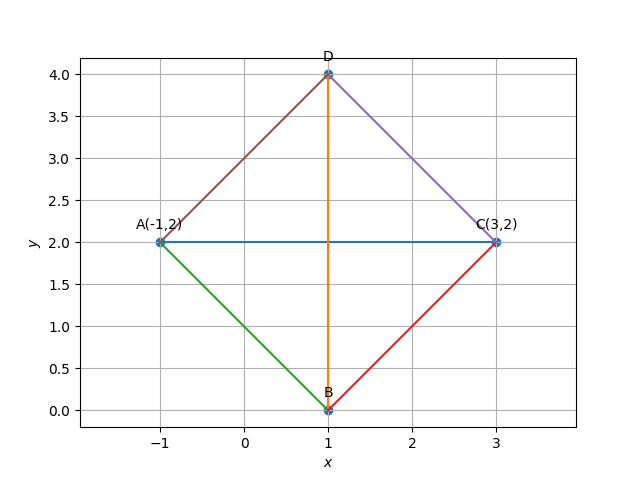
\includegraphics[width=\columnwidth]{chapters/10/7/4/4/figs/square}
	\end{center}
\caption{}
\label{fig:7/4/4/4Fig1}
\end{figure}

Shifting $\vec{A}$ to origin with reference to Fig. \ref{fig:7/4/4/4Fig2},
\begin{align}
\vec{A^{\prime}} =
\myvec{
0 \\
0\\
},
\vec{C^{\prime}} = \vec{C}-\vec{A} = 
\myvec{
4 \\
0\\
}
\end{align}

\begin{figure}[!h]
	\begin{center} 
	    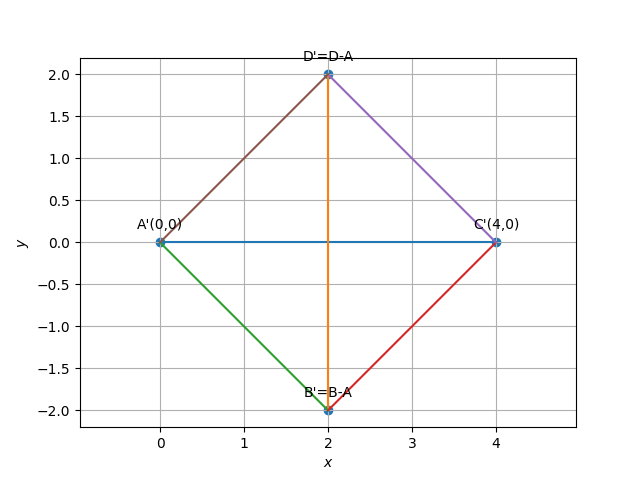
\includegraphics[width=\columnwidth]{chapters/10/7/4/4/figs/square1}
	\end{center}
\caption{}
\label{fig:7/4/4/4Fig2}
\end{figure}
\iffalse
In general,
the angle made by $AC$ with the x-axis is 
		\begin{align}
\beta = \theta + 45\degree
		\end{align}
\fi
Since
\begin{align}
\vec{C} - \vec{A} = \myvec{
4\\
0
} \equiv 
\myvec{
1\\
0
},
	\tan\theta&= \frac{0}{4} \implies 
\theta= 0\degree
\end{align}
		where
$\theta$ is the angle made by $AC$ with the x-axis.
Considering the rotation matrix 
\begin{align}
\vec{P} =
\myvec{
\cos\brak{\frac{\pi}{4}-\theta} & -\sin\brak{\frac{\pi}{4}-\theta} \\
\sin\brak{\frac{\pi}{4}-\theta} & \cos\brak{\frac{\pi}{4}-\theta} 
}
\end{align}
\iffalse
from Fig. \ref{fig:7/4/4/4Fig3},
\begin{align}
\vec{C^{\prime \prime}} = \vec{P}^\top (\vec{C}-\vec{A}) =
\myvec{
\frac{1}{\sqrt{2}} & -\frac{1}{\sqrt{2}} \\
\frac{1}{\sqrt{2}} & \frac{1}{\sqrt{2}}\\
}
\myvec{
4 \\
0\\
} = 
\myvec{
\frac{4}{\sqrt{2}} \\
\frac{4}{\sqrt{2}}\\
}
\end{align}
\begin{align}
\vec{B^{\prime \prime}} = \myvec{
 1&0\\
 0&0\\
}\vec{C^{\prime \prime}}=
\myvec{
 \frac{4}{\sqrt{2}}\\
 0\\
},
\vec{D^{\prime \prime}} = \myvec{
 0&0\\
 0&1\\
}\vec{C^{\prime \prime}}=
\myvec{
 0\\
 \frac{4}{\sqrt{2}}\\
} \text{ and }
\vec{A^{\prime \prime}} =
\myvec{
0 \\
0\\
}
\end{align}
\fi
\begin{figure}[!h]
	\begin{center} 
	    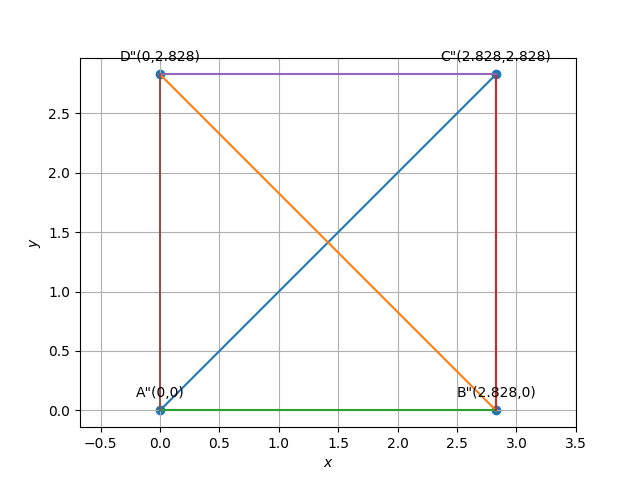
\includegraphics[width=\columnwidth]{chapters/10/7/4/4/figs/square2}
	\end{center}
\caption{}
\label{fig:7/4/4/4Fig3}
\end{figure}

\newpage
\iffalse
Again tranforming(rotating) the coordinates back to the original axis.

We know for anti-clockwise direction the rotation matrix is given as
\begin{align}
\vec{P} =
\myvec{
\cos\theta & -\sin\theta \\
\sin\theta & \cos\theta \\
}
\end{align}

Again we know that the angle is negative so the rotation will be in clockwise direction. So now the transformed(rotated) coordinates $\vec{B} \text{ and } \vec{D}$ are with refrence to 
\fi
from Figure 
%\ref{fig:7/4/4/4Fig4},
\ref{fig:7/4/4/4Fig3},
\begin{align}
	\vec{C^{\prime \prime}} &= \vec{P} (\vec{C}-\vec{A}) 
	\\
\label{eq:7/4/4/4bp}
	\vec{B^{\prime \prime}} &= \myvec{\vec{e}_1 & \vec{0}}\vec{C^{\prime \prime}}
	\\
\label{eq:7/4/4/4dp}
	\vec{D^{\prime \prime}} &= \myvec{ \vec{0} & \vec{e}_2}\vec{C^{\prime \prime}}
\end{align}
Now, 
\begin{align}
\label{eq:7/4/4/4b}
	\vec{B} = \vec{P}^{\top}\vec{B}^{\prime \prime}+\vec{A}
	\\
\label{eq:7/4/4/4d}
	\vec{D} = \vec{P}^{\top}\vec{D}^{\prime \prime}+\vec{A}
\end{align}
by reversing the process of translation and rotation.  Thus, 
from
\eqref{eq:7/4/4/4b}
\eqref{eq:7/4/4/4bp},
\eqref{eq:7/4/4/4d}
and
\eqref{eq:7/4/4/4dp}
\begin{align}
	\vec{B} = \vec{P}^{\top}\myvec{\vec{e}_1 & \vec{0}}\vec{P} (\vec{C}-\vec{A}) +\vec{A}
	\\
	\vec{D} = \vec{P}^{\top}\myvec{\vec{0} & \vec{e}_2  }\vec{P} (\vec{C}-\vec{A}) +\vec{A}
%	\vec{B} &= \brak{(\vec{C}-\vec{A})^{\top}\vec{P}^{\top} \vec{e}_1}\vec{P}^{\top}\vec{e}_1+\vec{A}
%	\\
%	\vec{D} &= \brak{(\vec{C}-\vec{A})^{\top}\vec{P}^{\top} \vec{e}_2}\vec{P}^{\top}\vec{e}_2+\vec{A}
\end{align}
yielding
		\begin{align}
\vec{B}=
\myvec{
1\\
0
},
\vec{D}
\myvec{
1\\
4
}.
		\end{align}
\iffalse
\begin{align}
\vec{B^{\prime}} &= \vec{P}\vec{B^{\prime \prime}} = \myvec{
\frac{1}{\sqrt{2}} & \frac{1}{\sqrt{2}} \\
-\frac{1}{\sqrt{2}} & \frac{1}{\sqrt{2}}\\
}
\myvec{
 \frac{4}{\sqrt{2}}\\
 0\\
} = 
\myvec{
2 \\
-2\\
}\\
\vec{D^{\prime}} &= \vec{P}\vec{D^{\prime \prime}} = \myvec{
\frac{1}{\sqrt{2}} & \frac{1}{\sqrt{2}} \\
-\frac{1}{\sqrt{2}} & \frac{1}{\sqrt{2}}\\
}
\myvec{
 0\\
 \frac{4}{\sqrt{2}}\\
} = 
\myvec{
2 \\
2 \\
}
\end{align}

\begin{figure}[!h]
	\begin{center} 
	    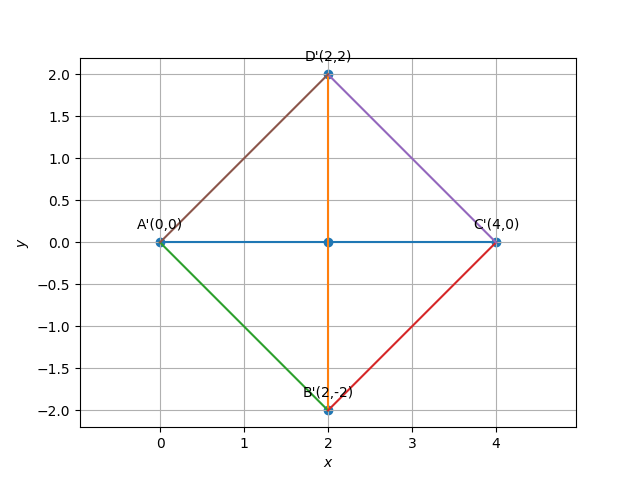
\includegraphics[width=\columnwidth]{chapters/10/7/4/4/figs/square3}
	\end{center}
\caption{}
\label{fig:7/4/4/4Fig4}
\end{figure}

Again transforming(shifting) the axis back to the original with refrence to Figure \ref{fig:7/4/4/4Fig5}
\begin{align}
\vec{B} &= \vec{B^{\prime}}+\vec{A} = \myvec{
2 \\
-2\\
}+\myvec{
-1 \\
2\\
} = 
\myvec{
1 \\
0\\
}\\
\vec{D} &= \vec{D^{\prime}}+\vec{A} = \myvec{
2 \\
2\\
}+\myvec{
-1 \\
2\\
} = 
\myvec{
1 \\
4 \\
}
\end{align}

Hence, the other two vertices are $\vec{B}(1,0) \text{ and } \vec{D}(1,4)$   

\begin{figure}[!h]
	\begin{center} 
	    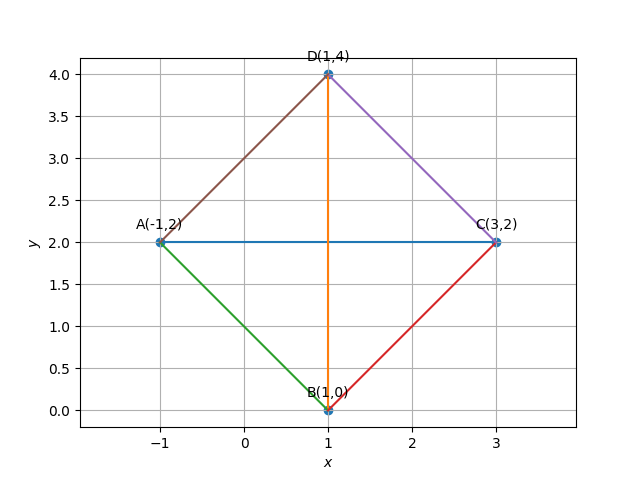
\includegraphics[width=\columnwidth]{chapters/10/7/4/4/figs/square4}
	\end{center}
\caption{}
\label{fig:7/4/4/4Fig5}
\end{figure}
which can also be expressed as
\begin{align}
\vec{B} &= \vec{A} + \vec{P}\myvec{
\vec{e_{1}}&\vec{0}\\
}
\vec{P}^\top \brak{\vec{C}-\vec{A}}\\
\vec{D} &= \vec{A} + \vec{P}\myvec{
\vec{0}&\vec{e_{2}}\\
}
\vec{P}^\top \brak{\vec{C}-\vec{A}}\\
\end{align}
where $\vec{P}$ is the rotation matrix and $\vec{A} \text{ and } \vec{C}$ are the position vectors of opposite vertices.

Derivation of the above formulas:

We know that after shifting the axis and rotating by the required angle any arbitrary square will be aligned with the x and y axis so that we can directly get the vectors $\vec{B} \text{ and } \vec{D}$ as follows
\begin{align}
\vec{C^{\prime\prime}} &= \vec{P}^\top \brak{\vec{C} - \vec{A}}\\
\vec{B^{\prime\prime}} &= \myvec{
\vec{e_{1}} & \vec{0}
}\vec{C^{\prime\prime}} = \myvec{
\vec{e_{1}} & \vec{0}
}\vec{P}^\top \brak{\vec{C} - \vec{A}}\\
\vec{B^{\prime}} &= \vec{P} \vec{B^{\prime\prime}}  = \vec{P}\myvec{
\vec{e_{1}} & \vec{0}
}\vec{P}^\top \brak{\vec{C} - \vec{A}}\\
\vec{B} &= \vec{A}+\vec{B^{\prime}}\\
 &= \vec{A} + \vec{P}\myvec{
\vec{e_{1}}&\vec{0}\\
}
\vec{P}^\top\brak{\vec{C}-\vec{A}}
\end{align}

Similarly for D it can be derived as
\begin{align}
\vec{C^{\prime\prime}} &= \vec{P}^\top \brak{\vec{C} - \vec{A}}\\
\vec{D^{\prime\prime}} &= \myvec{
\vec{0} & \vec{e_{2}}
}\vec{C^{\prime\prime}} = \myvec{
\vec{0} & \vec{e_{2}}
}\vec{P}^\top \brak{\vec{C} - \vec{A}}\\
\vec{D^{\prime}} &= \vec{P} \vec{D^{\prime\prime}} = \vec{P} \myvec{
\vec{0} & \vec{e_{2}}
}\vec{P}^\top \brak{\vec{C} - \vec{A}}\\
\vec{D} &= \vec{A}+\vec{D^{\prime}}\\
 &= \vec{A} + \vec{P}\myvec{
\vec{0}&\vec{e_{2}}\\
}
\vec{P}^\top\brak{\vec{C}-\vec{A}}
\end{align}


Verification of the above formula for the given question

\begin{align}
\vec{B} &= \myvec{
-1\\
2\\
}+\myvec{
\frac{1}{\sqrt{2}} & \frac{1}{\sqrt{2}} \\
-\frac{1}{\sqrt{2}} & \frac{1}{\sqrt{2}}\\
}\myvec{
 1&0\\
 0&0\\
}\myvec{
\frac{1}{\sqrt{2}} & -\frac{1}{\sqrt{2}} \\
\frac{1}{\sqrt{2}} & \frac{1}{\sqrt{2}}\\
}\myvec{
4\\
0\\
}\\
 &= \myvec{
-1\\
2\\
}+\myvec{
\frac{1}{\sqrt{2}} & \frac{1}{\sqrt{2}} \\
-\frac{1}{\sqrt{2}} & \frac{1}{\sqrt{2}}\\
}\myvec{
 1&0\\
 0&0\\
}\myvec{
\frac{4}{\sqrt{2}}\\
\frac{4}{\sqrt{2}}\\
}\\
 &= \myvec{
-1\\
2\\
}+\myvec{
\frac{1}{\sqrt{2}} & \frac{1}{\sqrt{2}} \\
-\frac{1}{\sqrt{2}} & \frac{1}{\sqrt{2}}\\
}\myvec{
\frac{4}{\sqrt{2}}\\
0\\
}\\
 &= \myvec{
-1\\
2\\
}+\myvec{
2\\
-2\\
}\\
 &= \myvec{
1\\
0\\
}\\
\vec{D} &= \myvec{
-1\\
2\\
}+\myvec{
\frac{1}{\sqrt{2}} & \frac{1}{\sqrt{2}} \\
-\frac{1}{\sqrt{2}} & \frac{1}{\sqrt{2}}\\
}\myvec{
 0&0\\
 0&1\\
}\myvec{
\frac{1}{\sqrt{2}} & -\frac{1}{\sqrt{2}} \\
\frac{1}{\sqrt{2}} & \frac{1}{\sqrt{2}}\\
}\myvec{
4\\
0\\
}\\
 &= \myvec{
-1\\
2\\
}+\myvec{
\frac{1}{\sqrt{2}} & \frac{1}{\sqrt{2}} \\
-\frac{1}{\sqrt{2}} & \frac{1}{\sqrt{2}}\\
}\myvec{
 0&0\\
 0&1\\
}\myvec{
\frac{4}{\sqrt{2}}\\
\frac{4}{\sqrt{2}}\\
}\\
 &= \myvec{
-1\\
2\\
}+\myvec{
\frac{1}{\sqrt{2}} & \frac{1}{\sqrt{2}} \\
-\frac{1}{\sqrt{2}} & \frac{1}{\sqrt{2}}\\
}\myvec{
0\\
\frac{4}{\sqrt{2}}\\
}\\
 &= \myvec{
-1\\
2\\
}+\myvec{
2\\
2\\
}\\
 &= \myvec{
1\\
4\\
}
\end{align}
\fi








\item The base of an equilateral triangle with side $2a$ lies along the y-axis such that the mid-point of the base is at the origin. Find vertices of the triangle.
\label{chapters/11/10/1/2}
\iffalse
\documentclass[journal,12pt,twocolumn]{IEEEtran}
\usepackage{graphicx}
\usepackage{listings}
\usepackage[utf8]{inputenc}
\usepackage{caption}
\usepackage{hyperref}
\usepackage[cmex10]{amsmath}
\usepackage{array}
\usepackage{gensymb}
\usepackage{booktabs}
\usepackage{etoolbox}
\patchcmd{\section}{\centering}{}{}{}
\providecommand{\norm}[1]{\left\lVert#1\right\rVert}
\providecommand{\abs}[1]{\left\vert#1\right\vert}
\let\vec\mathbf
\newcommand{\myvec}[1]{\ensuremath{\begin{pmatrix}#1\end{pmatrix}}}
\newcommand{\mydet}[1]{\ensuremath{\begin{vmatrix}#1\end{vmatrix}}}
\providecommand{\brak}[1]{\ensuremath{\left(#1\right)}}
\makeatletter
\newcommand\xleftrightarrow[2][]{%
  \ext@arrow 9999{\longleftrightarrowfill@}{#1}{#2}}
\newcommand\longleftrightarrowfill@{%
  \arrowfill@\leftarrow\relbar\rightarrow}
\makeatother
\title{Matrix Problems \textbf{\\Straight Lines }}
\author{Manoj Chavva} 

\begin{document}
\maketitle



\section{Problem Statement}

\noindent 
\fi
	\begin{figure}[!ht]
		\centering
 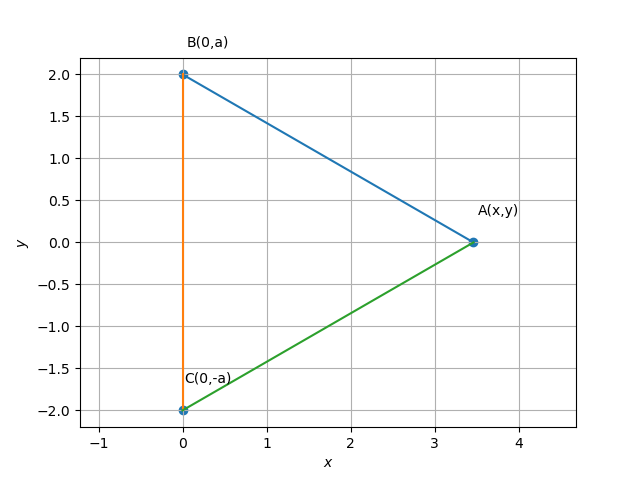
\includegraphics[width=\columnwidth]{chapters/11/10/1/2/figs/triangle.png}
		\caption{}
		\label{fig:11/10/1/2}
  	\end{figure}
	\\
	\solution Let the base be $BC$.  From the given information, 
\begin{align}
	\vec{B} = a\vec{e}_2,
	\vec{C} = -a\vec{e}_2
\end{align}
Since $\vec{A}$ lies on the $x$-axis, 
\begin{align}
	\vec{A} = k\vec{e}_1
\end{align}
and 
\begin{align}
	\norm{\vec{A}-\vec{C}}^2 &= \brak{2a}^2
	\\
	\implies \norm{\vec{A}}^2+\norm{\vec{C}}^2 - 2 \vec{A}^{\top}\vec{C} &= 4a^2
	\\
	\implies k^2 +a^2 &= 4a^2
	\\
	\text{or, } k = \pm a\sqrt{3}
\end{align}
Thus, 
\begin{align}
	\vec{A} = \pm \sqrt{3}a\vec{e}_1
\end{align}
		Fig. \ref{fig:11/10/1/2}
		is plotted for $a = 2$.

\iffalse

\begin{figure}[h]
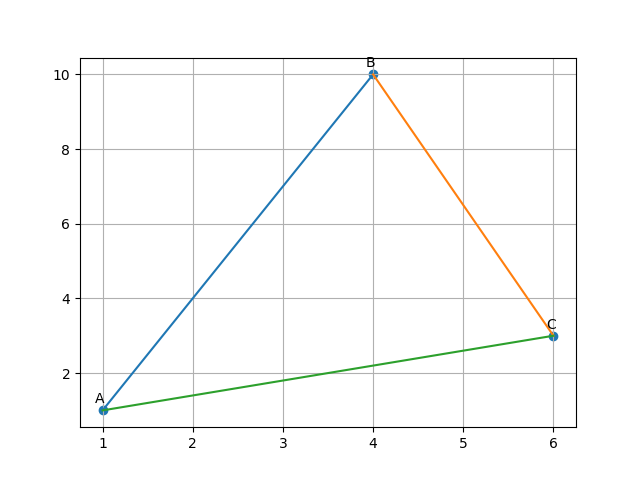
\includegraphics[width=1\columnwidth]{triangle.png}
\caption{Equilateral Triangle ABC}
\label{fig:triangle}
\end{figure}

\section{Construction}
B and C are the inputs.
\begin{table}[h]
\centering
\large
\begin{tabular}{|l|l|l|}
\hline
\textbf{Symbol} & \textbf{Value} & \textbf{Description} \\ \hline
B               & \myvec{0 \\ 2}         & Vertex B             \\ \hline
C               & \myvec{0 \\ -2}        & Vertex C             \\ \hline
A               & \myvec{x \\ y}          & Vertex A             \\ \hline
A1              & \myvec{x1 \\ y1}       & Vertex A             \\ \hline
\end{tabular}
\end{table}

\section{Solution}
\noindent Given the base with 2a is lies on the y-axis with the mid-point of the base is at origin. The vertices of the two points on y-axis will be

\begin{equation}
\vec{B}=\begin{pmatrix} 
0\\
a
\end{pmatrix}, {
\vec{C}=\begin{pmatrix} 
0\\
-a
\end{pmatrix} }
\end{equation}
\noindent Given $\Delta$ABC is an equilateral triangle i.e 
\begin{equation}
 \norm{\vec{A}-\vec{B}}= \norm{\vec{B}-\vec{C}}= \norm{\vec{C}-\vec{A}} =2a
\end{equation}

%\noindent As AB = AC, triangle is isoceles and by properties of isoceles triangle, altitude is perpendicular bisector of base.\\
%
%\noindent Therefore $\angle$AOC = $\angle$AOB = $90^0$ and $\norm{\vec{O}-\vec{B}}= \norm{\vec{O}-\vec{C}}= a$ \\
%
%\noindent By Cosine laws,
%\begin{equation}
%\cos\vec{B} = \cos\vec{C} = a* \frac{1}{2a} = \frac{1}{2}
%\end{equation}
%\begin{equation}
%\angle B = \angle C = \arccos\frac{1}{2} = 60^0
%\end{equation}
% \begin{equation}
% \angle A = 180^0 -(60^0 * 2) = 60^0
%  \end{equation}
%\noindent Therefore, the equilaterial triangle have all internal angles eaqual to  $60^0$ 

\noindent Consider, two sides of equilateral triangle be $\vec{A}$ and $\vec{B}$ then the third side will be $ \vec{A} -\vec{B}$ 
%Hence,
%\begin{equation}
%\norm{\vec{a}-\vec{b}}^2 = l
%\end{equation}
%\begin{equation}
%\brak{\vec{a}-\vec{b}}^{\top} \brak{\vec{a}-\vec{b}} = l^2
%\end{equation}
%\begin{equation}
%l^2 = 2 \vec{a}^{\top} \cdot \vec{b}
%\end{equation}
%\begin{equation}
%l^2 = 2 \norm{\vec{a}}\norm{\vec{b}} \cos\theta
%\end{equation}
%\begin{equation}
%\theta = \arccos\frac{1}{2} = 60^0
\begin{equation}
\norm{\vec{A}}=\norm{\vec{B}}=\norm{\vec{A-B}}\\
\end{equation}
\begin{equation}
\norm{\vec{A}}^2=\norm{\vec{B}}^2=\norm{\vec{A-B}}^2\\
\end{equation}
\begin{equation}
\norm{\vec{A}}^2+\norm{\vec{B}}^2-2\vec{A}^T\vec{B}=\norm{\vec{A}}^2=\norm{\vec{B}}^2\\
\end{equation}
\begin{equation}
\frac{\vec{A}^T\vec{B}}{\norm{\vec{A}}^2}=\frac{\vec{A}^T\vec{B}}{\norm{\vec{B}^2}}=\frac{1}{2}
\end{equation}
%$\triangle$OAB is a equilateral triangle\\

\noindent Therefore, the  triangle have all internal angles eaqual to  $60^0$

The angle between two vectors is given by 
  \begin{align}
    \label{eq:angle2d}
    \theta = \cos^{-1}\frac{\vec{A}^{\top} \vec{B}}{\norm{A}\norm{B}}
  \end{align}

 \begin{equation}  
  \brak{\vec{x}-\vec{B}}^{\top} \brak{\vec{x}-\vec{C}}= \norm{\vec{x}-\vec{B}} \cdot \norm{\vec{x}-\vec{C}} \cdot \cos\theta 
 \end{equation}

 \begin{equation}  
\brak{\vec{x}^\top \cdot \vec{x}} - \brak{\vec{x}^\top \cdot \vec{C}} - \brak{\vec{B}^\top \cdot \vec{x}} - \brak{\vec{B}^\top \cdot \vec{C}} = 2a \cdot 2a \cos 60^0   
 \end{equation}

 \begin{equation}  
\norm{\vec{x}}^2 - \vec{x}^\top\brak{\vec{B}+\vec{C}} - \vec{B}^\top \cdot \vec{C} = 2a \cdot 2a \cdot \frac{1}{2}
 \end{equation}

  \begin{equation}  
\norm{\vec{x}}^2 - \vec{x}^\top\brak{0} -\myvec{0 \\ a} \myvec{0 & -a}  = 4a^2
 \end{equation}

\begin{equation}
\norm{\vec{x}}^2 + a^2 = 4a^2
\end{equation}

\begin{equation}
\norm{\vec{x}}^2 = 3a^2
\label{eq-1}
\end{equation}
Considering, the line equation of $\vec{AB}$

\begin{equation}
\norm{\vec{x}-\vec{B}}^2 = 4a^2
\end{equation}

\begin{equation}
\brak{\vec{x} -\vec{B}}^{\top} \cdot \brak{\vec{x}-\vec{B}} = 4a^2
\end{equation}

\begin{equation}
\norm{\vec{x}}^2-2\cdot \vec{x}^\top \vec{B} + \norm{\vec{B}}^2 = 4a^2
\end{equation}

\begin{equation}
3a^2 - 2\cdot \vec{x}^\top \vec{B} + a^2 = 4a^2
\end{equation}

\begin{equation}
\vec{x}^\top \vec{B} = 0
\end{equation}
\noindent Since we can write, \begin{equation}
\vec{B} = a \cdot \vec{e}_2
\end{equation}

\begin{equation}
\vec{x}^\top \cdot a \cdot \vec{e}_2 = 0
\end{equation}

\begin{equation}
\vec{x}^\top \cdot \vec{e}_2 = 0
\end{equation}

\begin{equation}
\vec{x} = \lambda \vec{e}_1
\end{equation}

\noindent From this its clearly concluded that third vertex will lie on x-axis. 
\noindent From the equation \eqref{eq-1} 
\begin{equation}
\vec{x} = \sqrt{3}{a}
\end{equation}


\noindent Hence,the coordinates of the vertices of triangle are 
  \begin{equation*}
\vec{A} = 
   \begin{pmatrix}
   \pm\sqrt{3}a \\ 0
 \end{pmatrix}
 \end{equation*}

\begin{equation}
\vec{B}=\begin{pmatrix} 
0\\
a
\end{pmatrix}, {
\vec{C}=\begin{pmatrix} 
0\\
-a
\end{pmatrix} }
\end{equation}



\begin{table}[h]
\large
\begin{tabular}{lll}
\multicolumn{3}{l}{Get Python Code for image from}                                                 \\ \hline
\multicolumn{3}{|l|}{\url{https://github.com/ManojChavva/FWC/blob/main/Matrix/line/code-py/triangle.py}} \\ 
 \hline
\multicolumn{3}{l}{Get LaTex code from}                                                            \\ \hline
\multicolumn{3}{|l|}{\url{https://github.com/ManojChavva/FWC/blob/main/Matrix/line/line.tex}}            \\ \hline
\end{tabular}
\end{table}

\end{document}

\fi

\item The value of the expression $\abs{\vec{a}\times\vec{b}}$+ $({\vec{a}.\vec{b}})$ is \rule{1cm}{0.15mm}.
\item If $\abs{\vec{a}\times\vec{b}}^2$ + $\abs{\vec{a}.\vec{b}}^2$=144 $\text{and}$  $\abs{\vec{a}}$=4, then $\abs{\vec{b}}$ is equal to \rule{1cm}{0.15mm}.
\item If the directions cosines of a line are $(k,k,k)$ then
\begin{enumerate}
	\item $k>0$
	\item $0<k<1$
	\item $k=1$ 
	\item $k=\dfrac{1}{\sqrt{3}}$ or $-\dfrac{1}{\sqrt{3}}$
\end{enumerate}
\item  Find the position vector of a point A in space such that $\overrightarrow{OA}$ is inclined at $60 \degree$ to OX and at $45 \degree$ to OY and $\abs{\overrightarrow{OA}} =10$ units.
\item If $(-4,3)\text{ and }(4,3)$ are two vertices of an equilateral triangle. Find the coordinates of the third vertex, given that the origin lies in the interior of the triangle. 
\item $\vec{A} (6,1),\vec{B}(8,2) \text{ and } \vec{C}(9,4)$ are three vertices of a parallelogram ABCD. If $\vec{C}$ is the midpoint of DC find the area of $\triangle ADE$
\item If the points  $\vec{A}(1,-2), \vec{B}(2,3) , \vec{C}(a,2)\text{ and }\vec{D} (-4-3)$ form parallelogram, find the value of $a$ and height of the parallelogram taking AB as base.
\item Ayush starts walking from his house to office. Instead of going to the office directly, he goes to a bank first, from there to his daughter school and then reaches the office what is the extra distance travelled by Ayush in reaching his office? (Assume that all distanes covered are in straight lines). If the house is situated at $(2,4)$, bank at $(5,8)$, school at $(13,14)$ and office at $(13,26)$ and coordinates are in km.
\item Find the angle between the lines whose direction cosines are given by the equations $l+m+n=0$, $l^2+m^2-n^2=0$.
\item If a variable line in two adjacent positions has directions cosines $l, m, n$ and $l+\delta l, m+\delta m, n+\delta n$, show that the small angle $\delta\theta$ between the two positions is given by 
\begin{align}
	\delta\theta^2=\delta l^2+\delta m^2+\delta n^2
\end{align}
\item The vector $\vec{a}+\vec{b}$ bisects the angle between the non-collinear vectors $\vec{a}$ $\text{ and }$ $\vec{b}$ if \rule{1cm}{0.15mm}.
\item If $\vec{a}$ $\text{ and }$ $\vec{b}$ are adjacent sides of a rhombus, then $\vec{a}\cdot \vec{b}$=0.
\item Let $\vec{a}$ and $\vec{b}$ be two unit vectors and $\theta$ the angle between them. Then $\vec{a}+\vec{b}$ is a unit vector if
	\begin{enumerate}
			\itemsep2pt
		\item $\theta = \frac{\pi}{4}$
		\item $\theta = \frac{\pi}{3}$
		\item $\theta = \frac{\pi}{2}$
		\item $\theta = \frac{2\pi}{3}$
			\end{enumerate}
\solution
Given,
\begin{align}
	\norm{\vec{a}}=\norm{\vec{b}}=1\label{eq:12/10/5/17/1}
	\\
	\norm{\vec{a}+\vec{b}}=1\label{eq:12/10/5/17/2}
\end{align}
Squaring both sides of \eqref{eq:12/10/5/17/2}  , we get
\begin{align}
	\norm{\vec{a}+\vec{b}}^2=1^2
\\	
	\implies \norm{\vec{a}}^2 + \norm{\vec{b}}^2 + 2\vec{a}^{\top}\vec{b} = 1\label{eq:12/10/5/17/3}	
\end{align}
Substituting \eqref{eq:12/10/5/17/1} in \eqref{eq:12/10/5/17/3}, we get
\\
\begin{align}
	\implies 1+1+2(\norm{\vec{a}}\norm{\vec{b}}\cos{\theta})=1
	\\
	\implies 2+2(\norm{\vec{a}}\norm{\vec{b}}\cos{\theta})=1
        \\
	\implies 2(\norm{\vec{a}}\norm{\vec{b}}\cos{\theta})=-1
	\\
	\implies (\norm{\vec{a}}\norm{\vec{b}}\cos{\theta})=\frac{-1}{2}\label{eq:12/10/5/17/4}
\end{align}
Subtituting \eqref{eq:12/10/5/17/1} in \eqref{eq:12/10/5/17/4}, we get
\begin{align}
	\implies \cos{\theta}=\frac{-1}{2}
	\\
	\implies \theta=\frac{2\pi}{3}
\end{align}

\item Show that the tangent of an angle between the lines 
\begin{align}
	\frac{x}{a}+\frac{y}{b}&=1 \text{ and }
	\\
	\frac{x}{a}-\frac{y}{b}&=1 
\end{align}
is $\frac{2ab}{a^2-b^2}$.
\item Find $\abs{\overrightarrow {x}}$, if for a unit vector $\overrightarrow {a}, (\overrightarrow {x}-\overrightarrow {a})\cdot (\overrightarrow {x}+\overrightarrow {a}$)=12.
	\\
\solution 
		From the given information,
\begin{align}
  \label{eq:12/10/3/9det2f}
  \brak{\vec{x}-\vec{a}}^\top\brak{\vec{x}+\vec{a}} &= 12 \\
  \implies \norm{\vec{x}}^{2} - \norm{\vec{a}}^{2} &= 12 \\
\implies   
	\norm{\vec{x}} &= \sqrt{13}
\end{align}

\item Find $\abs{\overrightarrow {a}}$ and $\abs{\overrightarrow {b}}$, if ($\overrightarrow {a}+\overrightarrow {b})\cdot (\overrightarrow {a}-\overrightarrow {b})=8$ and $\abs{\overrightarrow {a}}=8\abs{\overrightarrow {b}}$.
	\\
	\solution
		\begin{align}
\because \brak{\vec{a}+\vec{b}}^\top\brak{\vec{a}-\vec{b}}=8,
\norm{\vec{a}} &= 8\norm{\vec{b}},\\
\norm{\vec{a}}^2-\norm{\vec{b}}^2&=8\\
\implies\norm{8\vec{b}}^2-\norm{\vec{b}}^2&=8\\
\implies \norm{\vec{b}}&=\frac{2\sqrt{2}}{3\sqrt{7}}
\end{align}
Thus, 
\begin{align}
\norm{\vec{a}}&=8\norm{\vec{b}}
=\frac{16\sqrt{2}}{3\sqrt{7}}
\end{align}

\item Find the magnitude of two vectors $\overrightarrow {a}$ and $\overrightarrow {b}$, having the same magnitude and such that the angle between them is $60\degree$ and their scalar product is $\frac{1}{2}$.
	\\
	\solution
		Given 
\begin{align}
	\norm{\vec{a}}= \norm{\vec{b}}, {\cos\theta} = \frac{1}{2}, 
	\vec{a}^{\top}{\vec{b}} = \frac{1}{2},  \\
\implies 
	\frac{1}{2} = \frac{\frac{1}{2}}{\norm{\vec{a}}^2}
\implies \norm{\vec{a}}
= \norm{\vec{b}}=1
\end{align}
by using  the definition of the scalar product.

\item Show that $\abs {\overrightarrow {a}}\overrightarrow {b}+\abs{\overrightarrow {b}}\overrightarrow {a}$ is perpendicular to $\abs{\overrightarrow {a}} \overrightarrow {b}-\abs{\overrightarrow {b}} \overrightarrow {a}$, for any two nonzero vectors $\overrightarrow {a}$ and $\overrightarrow {b}$.
	\\
	\solution
		\begin{align}
\norm{\vec{a}}\vec{b}+\norm{\vec{b}}\vec{a}
=
	\norm{\vec{a}}\norm{\vec{b}}\brak{\frac{\vec{b}}{\norm{\vec{b}}}+\frac{\vec{a}}{\norm{\vec{a}}}}
	\\
\norm{\vec{a}}\vec{b}-\norm{\vec{b}}\vec{a}
=
	\norm{\vec{a}}\norm{\vec{b}}\brak{\frac{\vec{b}}{\norm{\vec{b}}}-\frac{\vec{a}}{\norm{\vec{a}}}}
	\\
	\implies 
	\brak{\norm{\vec{a}}\vec{b}+\norm{\vec{b}}\vec{a}}^{\top} \brak{\norm{\vec{a}}\vec{b}-\norm{\vec{b}}\vec{a}} = 0
\end{align}
	from \eqref{eq:12/10/3/11/unit}.

\item If $\overrightarrow {a},\overrightarrow {b},\overrightarrow {c}$ are unit vectors such that $\overrightarrow {a}+\overrightarrow {b}+\overrightarrow {c}=\overrightarrow {0}$, find the value of $\overrightarrow {a}.\overrightarrow {b}+\overrightarrow {b}.\overrightarrow {c}+\overrightarrow {c}.\overrightarrow {a}$.
	\\
	\solution
		\begin{align}
	\norm{{\vec{a}}+{\vec{b}}+{\vec{c}}}^2=0
	\nonumber \\
	\implies{\norm{\vec{a}}}^2+{\norm{\vec{b}}}^2+{\norm{\vec{c}}}^2+2({{\vec{a}^\top}{\vec{b}}+{\vec{b}^\top}{\vec{c}}+{\vec{c}^\top}{\vec{a}}})=0
	\nonumber \\
	\implies3+2({{\vec{a}^\top}{\vec{b}}+{\vec{b}^\top}{\vec{c}}+{\vec{c}^\top}{\vec{a}}})=0\nonumber \\
	\implies{\vec{a}^\top}{\vec{b}}+{\vec{b}^\top}{\vec{c}}+{\vec{c}^\top}\vec{a}=-\frac{3}{2}
\end{align}

\item If either vector $\overrightarrow {a}=0$ or $\overrightarrow {b}=0$, then $\overrightarrow {a}.\overrightarrow {b}$=0. But the converse need not be true. Justify your answer with an example.
	\\
	\solution
		\begin{align}
	\vec{a}=\myvec{1\\1},\,
\vec{b}=\myvec{1\\-1}\\
\implies \vec{a} ^\top \vec{b} =  0 
\end{align}



\item Prove that $(\vec{a}+\vec{b})\cdot(\vec{a}+\vec{b})=|{\vec{a}}|^2+|{\vec{b}}|^2$, if and only if $\vec{a}, \vec{b}$ are perpendicular, given $\vec{a}\neq\vec{0}, \vec{b}\neq\vec{0}$.\\
	\solution
			\begin{align}
\because 		\brak{\vec{a}+\vec{b}}^{\top}\brak{\vec{a}+\vec{b}} 
		= \norm{\vec{a}}^2+\norm{\vec{b}}^2,
		\\
		 \norm{\vec{a}}^2+\norm{\vec{b}}^2+2\vec{a}^{\top}\vec{b}
		= \norm{\vec{a}}^2+\norm{\vec{b}}^2
		\\
		\implies 
		\vec{a}^{\top}\vec{b} = 0 
	\end{align}


	\item  If $l_1, m_1,n_1 \text{ and } l_2,m_2,n_2$ are the direction cosines of two mutually perpendicular lines, show that the direction cosines of the line perpendicular to both these are  $m_1n_2-m_2n_1,n_1l_2-n_2l_1,l_1m_2-l_2m_1$.
\\
    \solution
		\begin{align}
\vec{P} 
	=\myvec{
l_1&l_2&m_1n_2-m_2n_1\\
        m_1&m_2&n_1l_2-n_2l_1\\
        n_1&n_2&l_1m_2-l_2m_1
}
	\end{align}
	satisfies 
\eqref{eq:12/10/3/5/inner}.
	Hence, the three vectors are mutually perpendicular.

    \item If $ \vec{A},\vec{B},\vec{C} $ are mutually perpendicular vectors of equal magnitudes,show that the  $ \vec{A}+\vec{B}+\vec{C} $ is equally inclined to $ \vec{A},\vec{B}  \text{ and }  \vec{C} $.
\item Projection vector of $\vec{a}$ on $\vec{b}$ is
	\begin{enumerate}
\item $\left(\frac{\vec{a}\cdot\vec{b}}{\abs{\vec{b}}^2}\right)$
\item $\frac{\vec{a}\cdot\vec{b}}{\abs{\vec{b}}}$
\item $\frac{\vec{a}\cdot\vec{b}}{\abs{\vec{a}}}$
\item $\left(\frac{\vec{a}\cdot\vec{b}}{\abs{\vec{a}}^2}\right)$
\end{enumerate}
\item If $\vec{a}$ is  any non-zero vector, then $(\vec{a}\cdot \hat{i})\hat{i}$+$(\vec{a}\cdot \hat{j})\hat{j}$+$(\vec{a}\cdot \hat{k})$ $\hat{k}$ equals \rule{1cm}{0.15mm}.
\item If $\vec{a}$, $\vec{b}$, $\vec{c}$ are unit vectors such that $\vec{a}$+$\vec{b}$+$\vec{c}$=0, then the value of $\vec{a} \cdot \vec{b}+\vec{b} \cdot \vec{c}+\vec{c} \cdot \vec{a}$ is
	\begin{enumerate}
\item 1
\item 3
\item $\frac{-3}{2}$
\item None of these
\end{enumerate}
\item If $\vec{a},\vec{b},\vec{c}$ are the three vectors such that $\vec{a}+\vec{b}+\vec{c}=0$ $\text{ and }$ $|\vec{a}|=2$, $|\vec{b}|$=3, $|\vec{c}|$=5, the value of $\vec{a} \cdot \vec{b}+\vec{b} \cdot \vec{c}+\vec{c} \cdot \vec{a}$ is
	\begin{enumerate}
\item 0
\item 1	
\item -19
\item 38
\end{enumerate}
\item If $\vec{r}\cdot\vec{a}=0, \vec{r}\cdot\vec{b}=0$ and $\vec{r}\cdot\vec{c}=0$ for some non-zero vector $\vec{r}$, then the value of $\vec{a}\cdot(\vec{b}\times\vec{c})$ is \rule{1cm}{0.15mm}.
\item If $\abs{\vec{a}+\vec{b}}$ = $\abs{\vec{a}-\vec{b}}$, then the vectors $\vec{a}$ $\text {and}$ $\vec{b}$ are orthogonal.
\item Prove that the lines $x=py+q , z=ry+s \text{ and } x=p^{\prime}y+q^{\prime}, z=r^{\prime}y+s^{\prime} $ are perpendicular if $pp^{\prime}+rr^{\prime}+1=0$.
\item Show that the straight lines whose direction cosines are given by $2l+2m-n=0$ and $mn+nl+lm=0$ are at right angles.
\item If $l_1, m_1, n_1;l_2, m_2, n_2;l_3, m_3, n_3$ are the direction cosines of the three mutually perpendcular lines, prove that the line whose direction cosines are propotional to $l_1+l_2+l_3 , m_1+m_2,m_3, n_1+n_2+n_3$ make angles with them.
\item
Find the angle between the lines whose direction ratios are $a,b,c$ and $b-c,c-a,a-b$.
\\
\solution
    \begin{align}
\because \myvec{a&b&c}\myvec{b-c\\c-a\\a-b} = 0,
   \theta=\frac{\pi}{2}
    \end{align}

\end{enumerate}

\subsection{CBSE}
\begin{enumerate}[label=\thesubsection.\arabic*,ref=\thesubsection.\theenumi]
    \item Jagdish has a field which is in the shape of a right-angled triangle $ AQC $. He wants to leave a space in the form of a square $ PQRS $ inside the field for growing wheat and the remaining space for growing vegetables.  In the field, there is a pole marked as $ \vec{O} $.
    Based on the above information, answer the following equations
    \begin{enumerate}
        \item Taking $ \vec{O} $ as the origin, $ \vec{P} = (-200,0) $ and  $ \vec{Q} = (200,0) $. PQRS being a square, what are the coordinates of $ \vec{R} $ and $ \vec{S} $?
        \item
        \begin{enumerate}
            \item What is the area of square $ PQRS $?
            \item What is the length of diagonal $ PR $ in $ PQRS $?
        \end{enumerate}
        \item If $ \vec{S} $ divides $ CA $ in the ratio $ K:1 $, what is the value of $ K $, where $ \vec{A} = (200,800) $?
    \end{enumerate}
    \hfill (10, 2023)
    \item If $(-5,3)$ and $(5,3)$ are two vertices of an equilateral triangle, then the coordinates of the third vertex, given that the origin lies inside the triangle (take $\sqrt{3} = 1.7$), are
    \hfill (10, 2023)
    \item If
    \begin{align*}
        \left| \overrightarrow{a} \times \overrightarrow{b} \right|^2 + \left| \overrightarrow{a} \cdot \overrightarrow{b} \right|^2 = 400
    \end{align*}
    and
    \begin{align*}
        \left| \overrightarrow{b} \right| = 5,
    \end{align*}
    find the value of $\left| \overrightarrow{a} \right|$.
    \hfill (12, 2022)
    \item If
    \begin{align*}
        \overrightarrow{a} = \hat{i} + \hat{j} + \hat{k},
    \end{align*}
    \begin{align*}
        \overrightarrow{a} \cdot \overrightarrow{b} = 1,
    \end{align*}
    and
    \begin{align*}
        \overrightarrow{a} \times \overrightarrow{b} = \hat{j} - \hat{k},
    \end{align*}
    then find $\left| \overrightarrow{b} \right|$.
    \hfill (12, 2022)
    \item If
    \begin{align*}
        \left| \overrightarrow{a} \right| = 3,
    \end{align*}
    \begin{align*}
        \left| \overrightarrow{b} \right| = 2\sqrt{3},
    \end{align*}
    and
    \begin{align*}
        \overrightarrow{a} \cdot \overrightarrow{b} = 6,
    \end{align*}
    then find the value of $\left| \overrightarrow{a} \times \overrightarrow{b} \right|$.
    \hfill (12, 2022)

    \item $\left| \overrightarrow{a} \right| = 8$, $\left| \overrightarrow{b} \right| = 3$, and $\overrightarrow{a} \cdot \overrightarrow{b} = 12\sqrt{3}$, then the value of $\left| \overrightarrow{a} \times \overrightarrow{b} \right|$ is
    \hfill (12, 2022)
    \item If
    \begin{align*}
        \overrightarrow{a} = 2\hat{i} + \hat{j} + 3\hat{k},
    \end{align*}
    \begin{align*}
        \overrightarrow{b} = -\hat{i} + 2\hat{j} + \hat{k},
    \end{align*}
    and
    \begin{align*}
        \overrightarrow{c} = 3\hat{i} + \hat{j} + 2\hat{k},
    \end{align*}
    then find $\overrightarrow{a} \cdot (\overrightarrow{b} \times \overrightarrow{c})$.
    \hfill (12, 2022)

    \item $\overrightarrow{a}, \overrightarrow{b}, \overrightarrow{c},$ and $\overrightarrow{d}$ are four non-zero vectors such that
    \begin{align*}
        \overrightarrow{a} \times \overrightarrow{b} = \overrightarrow{c} \times \overrightarrow{d}
    \end{align*}
    and
    \begin{align*}
        \overrightarrow{a} \times \overrightarrow{c} = 4\overrightarrow{b} \times \overrightarrow{d},
    \end{align*}
    then show that $(\overrightarrow{a} - 2\overrightarrow{d})$ is parallel to $(2\overrightarrow{b} - \overrightarrow{c})$ where
    \begin{align*}
        \overrightarrow{a} \neq 2\overrightarrow{d}, \quad \overrightarrow{c} \neq 2\overrightarrow{b}.
    \end{align*}
    \hfill (12, 2022)

    \item If
    \begin{align*}
        \overrightarrow{a} = \hat{i} + \hat{j} + \hat{k},
    \end{align*}
    \begin{align*}
        \overrightarrow{a} \cdot \overrightarrow{b} = 1,
    \end{align*}
    and
    \begin{align*}
        \overrightarrow{a} \times \overrightarrow{b} = \hat{j} - \hat{k},
    \end{align*}
    then find $\left| \overrightarrow{b} \right|$.
    \hfill (12, 2022)

    \item If $\overrightarrow{a}$ and $\overrightarrow{b}$ are two vectors such that
    \begin{align*}
        \left| \overrightarrow{a} + \overrightarrow{b} \right| = \left| \overrightarrow{b} \right|,
    \end{align*}
    then prove that $(\overrightarrow{a} + 2\overrightarrow{b})$ is perpendicular to $\overrightarrow{a}$.
    \hfill (12, 2022)

    \item If $\overrightarrow{a}$ and $\overrightarrow{b}$ are unit vectors and $\theta$ is the angle between them, then prove that
    \begin{align*}
        \sin \frac{\theta}{2} = \frac{1}{2} \left| \overrightarrow{a} - \overrightarrow{b} \right|.
    \end{align*}
    \hfill (12, 2022)

    \item If $\overrightarrow{a}$ and $\overrightarrow{b}$ are two unit vectors and $\theta$ is the angle between them, then prove that
    \begin{align*}
        \sin \frac{\theta}{2} = \frac{1}{2} \left| \overrightarrow{a} - \overrightarrow{b} \right|.
    \end{align*}
    \hfill (12, 2022)
    \item If $\overrightarrow{a}$, $\overrightarrow{b}$, and $\overrightarrow{c}$ are the position vectors of the points $\vec{A}(2, 3, -4)$, $\vec{B}(3, -4, -5)$, and $\vec{C}(3, 2, -3)$ respectively, then $\left| \overrightarrow{a} + \overrightarrow{b} + \overrightarrow{c} \right|$ is equal to:
    \hfill (12, 2022)
    \item The two adjacent sides of a parallelogram are represented by $2\hat{i} + 4\hat{j} - 5\hat{k}$ and $\hat{i} + 2\hat{j} + 3\hat{k}$. Find the unit vectors parallel to its diagonals. Using the diagonal vectors, find the area of the parallelogram also.
    \hfill (12, 2022)
    \item If the points $\vec{A}(2,0)$, $\vec{B}(6,1)$, and $\vec{C}(p, q)$ form a triangle of area 12 square units (positive only) and
    \begin{align*}
        2p + q = 10,
    \end{align*}
    then find the values of $p$ and $q$.
    \hfill (10, 2022)
	\item Prove that three points $A$, $B$, and $C$ with position vectors $\vec{a}$, $\vec{b}$, and $\vec{c}$ respectively are collinear if and only if $(\vec{b} \times \vec{c}) + (\vec{c} \times \vec{a}) + (\vec{a} \times \vec{b}) = \vec{0}$. \hfill (12, 2021)
	\item If $|\overrightarrow{a}| = 2$, $|\overrightarrow{b}| = 7$, and $\overrightarrow{a} \times \overrightarrow{b} = 3\hat{i} + 2\hat{j} + 6\hat{k}$, find the angle between $\overrightarrow{a}$ and $\overrightarrow{b}$. \hfill (12, 2019)
	
	\item Find the volume of a cuboid whose edges are given by $-3\hat{i} + 7\hat{j} + 5\hat{k}$, $-5\hat{i} + 7\hat{j} - 3\hat{k}$, and $7\hat{i} - 5\hat{j} - 3\hat{k}$. \hfill (12, 2019)
	
	\item Let $\overrightarrow{a}$, $\overrightarrow{b}$, and $\overrightarrow{c}$ be three vectors such that $|\overrightarrow{a}| = 1$, $|\overrightarrow{b}| = 2$, and $|\overrightarrow{c}| = 3$. If the projection of $\overrightarrow{b}$ along $\overrightarrow{a}$ is equal to the projection of $\overrightarrow{c}$ along $\overrightarrow{a}$, and $\overrightarrow{b}$ and $\overrightarrow{c}$ are perpendicular to each other, then find $|3\overrightarrow{a} - 2\overrightarrow{b} + 2\overrightarrow{c}|$. \hfill (12, 2019)
	\item For any two vectors $\overrightarrow{\vec{a}}$ and $\overrightarrow{\vec{b}}$, prove that
	\begin{align*}
	|\overrightarrow{\vec{a}} \times \overrightarrow{\vec{b}}|^2 = \overrightarrow{\vec{a}}^2 \overrightarrow{\vec{b}}^2 - (\overrightarrow{\vec{a}} \cdot \overrightarrow{\vec{b}})^2.
	\end{align*} \hfill (12, 2019)
	\item $X$ and $Y$ are two points with position vectors $3\overrightarrow{a} + \overrightarrow{b}$ and $\overrightarrow{a} - 3\overrightarrow{b}$, respectively. Write the position vector of a point $Z$ which divides the line segment $XY$ in the ratio $2:1$ externally. \hfill (12, 2019)
\item Let $\overrightarrow{\mathbf{a}} = 4\hat{i} + 5\hat{j} - \hat{k}$, $\overrightarrow{\mathbf{b}} = \hat{i} - 4\hat{j} + 5\hat{k}$, and $\overrightarrow{\mathbf{c}} = 3\hat{i} + \hat{j} - \hat{k}$. Find a vector $\overrightarrow{\mathbf{d}}$ which is perpendicular to both $\overrightarrow{\mathbf{c}}$ and $\overrightarrow{\mathbf{b}}$ and satisfies $\overrightarrow{\mathbf{d}} \cdot \overrightarrow{\mathbf{a}} = 21$. \hfill (12, 2018)
\item Let $\overrightarrow{a}$, $\overrightarrow{b}$, and $\overrightarrow{c}$ be three vectors such that $|\overrightarrow{a}| = 1$, $|\overrightarrow{b}| = 2$, and $|\overrightarrow{c}| = 3$. If the projection of $\overrightarrow{b}$ along $\overrightarrow{a}$ is equal to the projection of $\overrightarrow{c}$ along $\overrightarrow{a}$, and $\overrightarrow{b}$ and $\overrightarrow{c}$ are perpendicular to each other, then find $|3\overrightarrow{a} - 2\overrightarrow{b} + 2\overrightarrow{c}|$. \hfill (12, 2018)
\item Given that vectors $\overrightarrow{a}$, $\overrightarrow{b}$, $\overrightarrow{c}$ form a triangle such that
      $\overrightarrow{a} = \overrightarrow{b}+\overrightarrow{c}$. Find $p$, $q$, $r$, $s$ such that area of triangle is $5\sqrt{6}$ where $\overrightarrow{a} = p\hat{i} +q\hat{j}+r\hat{k}$,
      $\overrightarrow{b} = s\hat{i} +3\hat{j}+4\hat{k}$ and $\overrightarrow{c}=3\hat{i} +\hat{j}-2\hat{k}$. \hfill (12, 2016)
\item Find the co-ordinates of the point where the line $\overrightarrow{r}=(-\hat{i}-2\hat{j}-3\hat{k})+\lambda(3\hat{i} +4\hat{j}+3\hat{k})$ meets the plane which is perpendicular to the vector $\overrightarrow{n}=\hat{i}+\hat{j} +3\hat{k}$ and at a distance of
      $\frac{4}{\sqrt{11}}$ from origin. \hfill (12, 2016)
\item Find a unit vector perpendicular to each of the vectors $(\vec{a}+\vec{b})$ and $(\vec{a}-\vec{b})$ where 
\begin{align}
	\vec{a}&=\hat{i}+\hat{j}+\hat{k}\\
	\vec{b}&=\hat{i}+2\hat{j}+3\hat{k}
\end{align}
\hfill (12, 2022)
\end{enumerate}

\newpage
\section{Constructions}
\subsection{Formulae}
\begin{enumerate}[label=\thesubsection.\arabic*.,ref=\thesubsection.\theenumi]
\item Construct a $\triangle ABC$ given $a, \angle B$ and $K = b+c$.
		\label{prob:9/11/2/1}
	\\
	\solution 
	Using the cosine formula in  $\triangle ABC$,
\begin{align}
	{b}^2&= {a}^2 + {c}^2 - 2ac\cos{B}
\\
\implies	(K-c)^2 &= {a}^2 + c^2- 2  a  c\cos{B}
\\
\implies
	c &=
	\frac{K^2-a^2}{2\brak{K- a  \cos{B}}}
		\label{eq:9/11/2/1}
\end{align}
The coordinates of $\triangle ABC$ can then be expressed as
\begin{align}
		\label{eq:9/11/2/1-final}
	\vec{A}=c\myvec{\cos B \\ \sin B},
	\vec{B} = \vec{0},
	\vec{C} =\myvec{a \\ 0}.
\end{align}
\item Construct a $\triangle ABC$ given $\angle B, \angle C$ and $K = a+b+c$.
	\\
	\solution
	\begin{align}
a+b+c &= K \\
b\cos C + c \cos B -a &=0 \\
b\sin C - c \sin B &=0
\end{align}
resulting in the matrix equation
\begin{align}
		\label{eq:9/11/2/4}
	\myvec{1 & 1 & 1 \\ -1 & \cos C & \cos B  \\ 0 &\sin C & -\sin B } \myvec{a \\ b \\ c} = K \myvec{1 \\ 0 \\ 0}
\end{align}
which can be solved to obtain all the sides.  $\triangle ABC$ can then be plotted using
\begin{align}
\vec{A} = \myvec{a \\ b},\,
\vec{B} = \vec{0},\, 
\vec{C} = \myvec{a \\ 0}
		\label{eq:9/11/2/4-final}
\end{align}
\end{enumerate}

\subsection{Triangle}
\begin{enumerate}[label=\thesubsection.\arabic*,ref=\thesubsection.\theenumi]
\item Construct a triangle $ABC$ in which $BC=7cm, \angle{B}=75\degree$ and $AB + AC = 13 cm$.
\label{chapters/9/11/2/1}
	\\
	\solution 
		From 
		\eqref{eq:9/11/2/1}
		and 
		\eqref{eq:9/11/2/1-final},
		we obtain
		\figref{fig:9/11/2/1}.
		\iffalse
		See
\begin{lstlisting}
	codes/triangle/const-aBsum.py
\end{lstlisting}
\fi
	\begin{figure}[H]
		\centering
 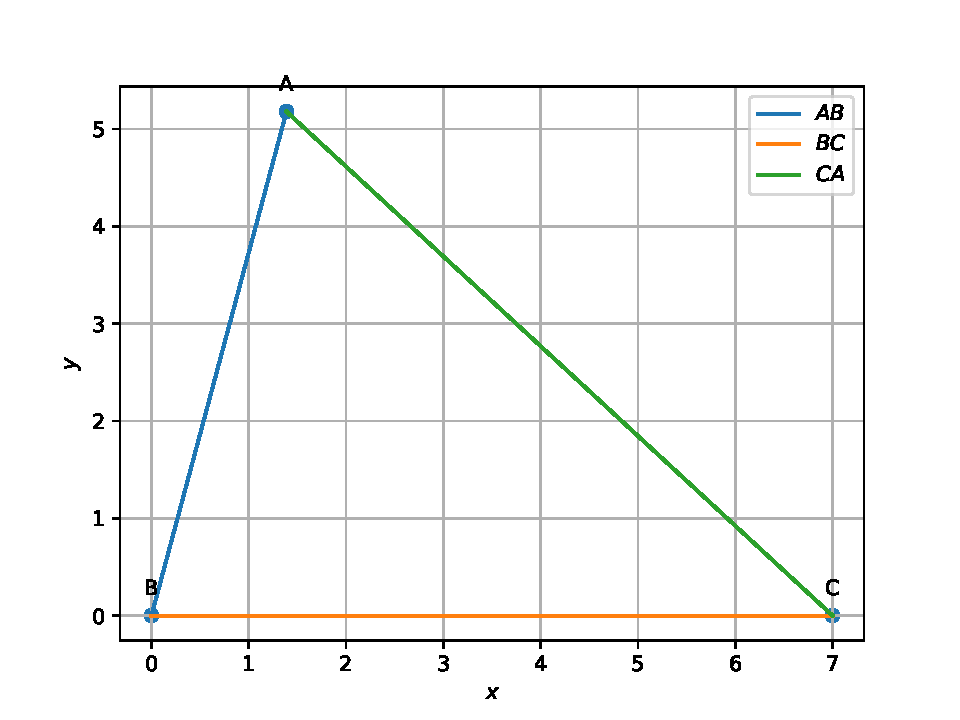
\includegraphics[width=0.75\columnwidth]{chapters/9/11/2/1/figs/vector.pdf}
		\caption{}
		\label{fig:9/11/2/1}
  	\end{figure}
	

%
\item Construct a triangle $ABC$ in which $BC=8cm, \angle{B}=45\degree$ and $AB - AC = 3.5 cm$.
\label{chapters/9/11/2/2}
\\
\solution
See \figref{fig:Fig1}.
\begin{figure}[H]
 \begin{center}
	 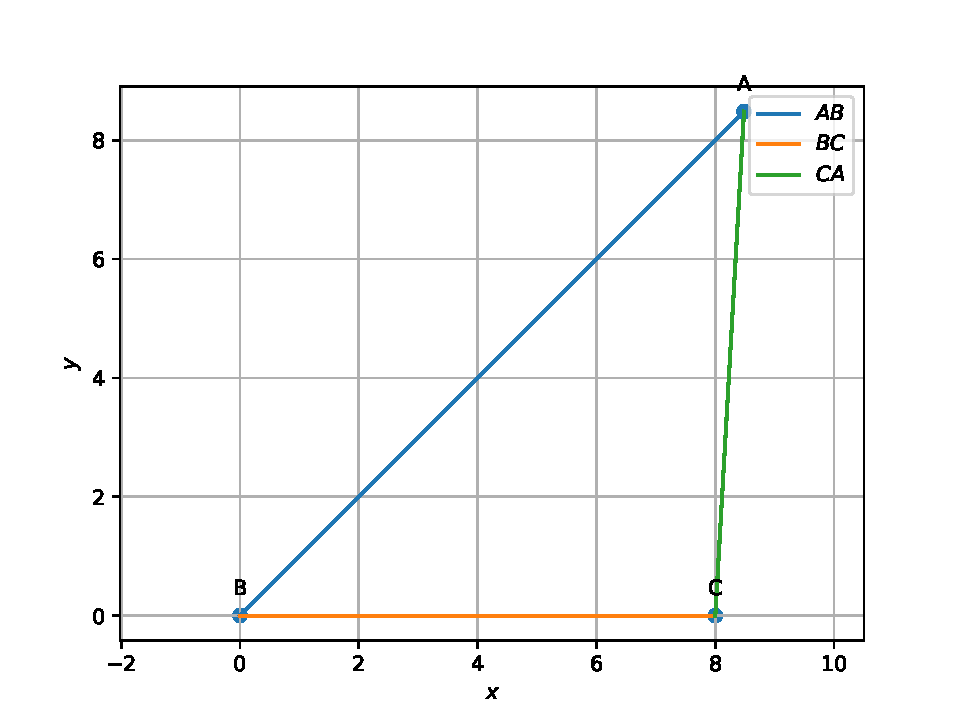
\includegraphics[width=0.75\columnwidth]{chapters/9/11/2/2/figs/vector.pdf}
 \end{center}
 \caption{}
 \label{fig:Fig1}
\end{figure}

%
\item Construct a triangle $ABC$ in which $BC=6cm, \angle{B}=60\degree$ and $AC - AB = 2cm$.
\label{chapters/9/11/2/3}
\\
\solution 
\iffalse
\documentclass[10pt,a4paper]{article}
\usepackage{amsmath}
\usepackage{amsfonts}
\usepackage{amssymb}
\usepackage{graphicx}
\usepackage{multicol}
\usepackage{tabularx}
\usepackage{tikz}
\usetikzlibrary{arrows,shapes,automata,petri,positioning,calc}
\usepackage{hyperref}
\usepackage{tikz}
\usepackage{gensymb}
\usepackage{polynom}
\usetikzlibrary{matrix,calc}
\makeatletter
\newcommand\xleftrightarrow[2][]{%
  \ext@arrow 9999{\longleftrightarrowfill@}{#1}{#2}}
\newcommand\longleftrightarrowfill@{%
  \arrowfill@\leftarrow\relbar\rightarrow}
\makeatother
\usepackage[margin=0.5in]{geometry}
\newcommand{\myvec}[1]{\ensuremath{\begin{pmatrix}#1\end{pmatrix}}}
\let\vec\mathbf
\newenvironment{Figure}
  {\par\medskip\noindent\minipage{\linewidth}}
  {\endminipage\par\medskip}
\begin{document}
%--------------------logo figure-------------------------%
\begin{figure*}[!tbp]
 \centering
  \begin{minipage}[b]{0.4\textwidth}
  
\includegraphics[scale=.25]{iitlogo.png} 
  \end{minipage}
\end{figure*}
%--------------------name & rollno-----------------------
\raggedright \textbf{Name}:\hspace{1mm} Ganga Gopinath\hspace{3cm} \Large \textbf{Matrix Assignment}\hspace{2.5cm} % 
\normalsize \textbf{Roll No.} :\hspace{1mm} FWC22050\vspace{1cm}
\begin{multicols}{2}
\section{Problem statement:}
\fi
	\begin{figure}[!h]
		\centering
 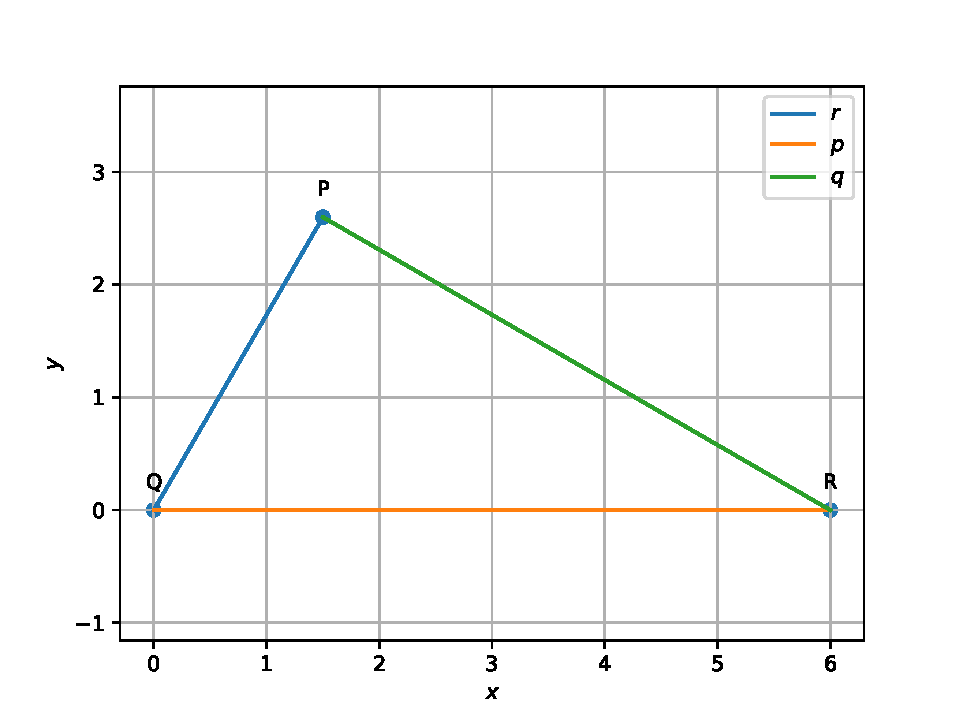
\includegraphics[width=\columnwidth]{chapters/9/11/2/3/figs/line1.pdf}
		\caption{}
		\label{fig:9/11/2/3}
  	\end{figure}
	\solution  Same as Problem 
\ref{chapters/9/11/2/1} with 
\begin{align}
\angle Q = \angle B, QR = a, PR = b, PQ = c
\end{align}
\iffalse

\textbf{Law of Cosines}
\vspace{2mm}\raggedright \\

The law of Cosines relates the length of the triangle to the cosines of one of its angles. It states that, if the length of two sides and the angle between them is known for a triangle, then we can determine the length of the third side. It is given by:
\begin{equation}
\alpha^2=\beta^2+\gamma^2-2\beta\gamma\cos\theta
\end{equation}
%-----------------------------solution---------------------------
\raggedright \textbf{SOLUTION}:\vspace{5mm}\\
\raggedright \textbf{Steps of Construction:}\vspace{2mm}\\
\textbf{Step 1:}\vspace{2mm}\\
Let P,Q and R be the vertices of the triangle  with coordinates.

Given QR length is a=6cm,
So the coordinates of vertices  Q,R and P are :\vspace{2mm}\\
\begin{center}$
{
 Q =\begin{pmatrix}
0 \\
0 
\end{pmatrix} 
\vspace{1mm}
R=\begin{pmatrix}
6 \\
0 
\end{pmatrix} 
\vspace{1mm}
P=\alpha\begin{pmatrix}
cos \theta\\
  sin \theta\\
\end{pmatrix} }
\vspace{1mm}$
\end{center}
Also given the angle is $Q=60^0$,so by finding the coordinates of the other sid
    e we can form a required triangle. \\
 \vspace{2mm}
For the input parameters in Table 1.\\
{\setlength\extrarowheight{2pt}
\begin{center}
\begin{tabular}{|c|c|c|}
	\hline
	\textbf{Symbol}&\textbf{Value}&\textbf{Description}\\
	\hline
	Q&$\begin{pmatrix}
	0\\0\\
	\end{pmatrix} $& Q Point\\
	\hline
	R&$\begin{pmatrix}
	6\\0\\
	\end{pmatrix} $& R Point\\
	\hline
	$\theta$&60$^{\circ}$&$\angle$PQR\\
	\hline
	$\lambda$ & 2 & PR-PQ\\
	\hline
	q&$\alpha$  & PR\\
	\hline
	r &$\gamma$  & PQ\\
	\hline
	p & 6 & QR\\
	\hline
\end{tabular}
%}\\
\\ {Table 1}\\
\end{center}
\vspace{3mm} 
Given that,
\begin{equation}
	\alpha-\gamma=2
\end{equation}
By using the Cosine formula in  $\Delta$PQR \\ 
\begin{equation}
\alpha^2=\beta^2+\gamma^2-2\beta\gamma\cos\theta 
\end{equation}
\vspace{1mm}
\begin{equation}
\alpha^2-\gamma^2=\beta^2-2\beta\gamma\cos\theta
\end{equation}
\vspace{1mm}
\begin{equation}
(\alpha+\gamma)(\alpha-\gamma)=\beta^2-2\beta\gamma\cos\theta
\end{equation}
\vspace{1mm}
\begin{equation}
(\alpha+\gamma)(\lambda)=\beta^2-2\beta\gamma\cos\theta
\end{equation}
\vspace{1mm}
\begin{equation}
\lambda\alpha +\lambda \gamma +2\beta\gamma\cos\theta=\beta^2
\end{equation}
\vspace{1mm}
\begin{equation}
\lambda \alpha +\gamma(\lambda+2\beta\cos\theta)=\beta^2
\end{equation}
\vspace{1mm}
%\begin{center}
%	$0=6^2+\gamma^2 -\alpha^2-2\times \gamma \times 6 \times cos60$\\

%\vspace{5mm}
%\end{center}
%After simplification
%\begin{equation}
%	   4\gamma+\alpha =18
%\end{equation}

\textbf{Step 2:}\vspace{2mm}\\
We know that,\\
\begin{equation}
\vec{A  X = B}
\end{equation}
Using equation (2) and (8),


\begin{equation}
  \begin{pmatrix}
1 & -1\\
\lambda & \lambda+2\beta\cos\theta
\end{pmatrix} 
\begin{pmatrix}
\alpha\\
\gamma
\end{pmatrix} 
=
\begin{pmatrix}
\lambda\\ 
 \beta^2\
\end{pmatrix}
\end{equation}\vspace{2mm}\\
 
After substituting values,
\begin{equation}
  \begin{pmatrix}
1 & -1\\
1 &4
\end{pmatrix} 
\begin{pmatrix}
\alpha\\
\gamma
\end{pmatrix} 
=
\begin{pmatrix}
2\\ 
 18\
\end{pmatrix}
\end{equation}\vspace{2mm}\\


The augmented matrix for the above matrix equation is 
\vspace{3mm}
\begin{equation}
\begin{pmatrix}
  1 & -1 & \vrule & 2\\
  1 & 4  &\vrule & 18
    \end{pmatrix}  
    \end{equation} 
    
  \begin{center}
  $ \xleftrightarrow{\text{$R_2$ $\leftarrow {R_2}-{R_1}$}} $
$\begin{pmatrix}
 1 & -1& \vrule & 2\\
 0 & 5  &\vrule & 16\
  \end{pmatrix}$
  \\
  \end{center}
  
  \begin{center}
$ \xleftrightarrow{\text{$R_2$ $\leftarrow  \frac{1}{5}{R_2}$}} $
$\begin{pmatrix}
 1 & -1 & \vrule & 2\\
  0 & 1  &\vrule & \frac{16}{5}\
  \end{pmatrix}$
  \\
  \end{center}    
  
  \begin{center}
  $ \xleftrightarrow{\text{$R_1$ $\leftarrow  {R_1}+{R_2}$}} $
$\begin{pmatrix}
  1 & 0 & \vrule & \frac{26}{5}\\
  0 & 1  &\vrule & \frac{16}{5}\
  \end{pmatrix}$
  \\
  \end{center}

  \begin{equation}
\implies X = 
   \begin{pmatrix}
   \frac {26}{5}\\ 
   \frac{16}{5}
 \end{pmatrix}
 \end{equation}
Using equation (7) we get ,
\begin{equation}
	\alpha = \frac{26}{5} \vspace{2mm}
\end{equation}
\begin{equation}
	\gamma= \frac{16}{5}\vspace{2mm}
\end{equation}
The vertices of $\Delta$ PQR are \\
\begin{equation}
P= \frac{26}{5} \begin{pmatrix}
cos 60\\
sin 60\\
\end{pmatrix} 
,Q= \begin{pmatrix}
 0\\
 0\\
 \end{pmatrix} 
,R= \begin{pmatrix}
 6\\
 0\\
\end{pmatrix} 
\end{equation} \vspace{2mm}


\textbf{Result} 
\begin{center}
	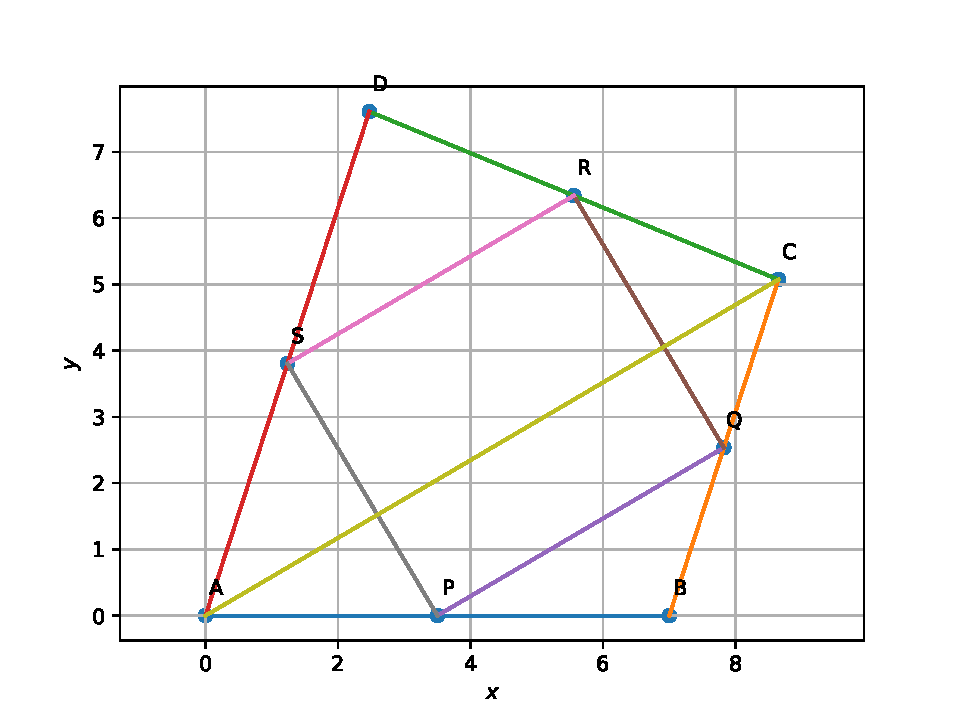
\includegraphics[width=0.4\textwidth]{line1.pdf}
\end{center}\vspace{5mm}

\vspace{4mm}  
\textbf{Implementation}
\begin{center}
\setlength{\arrayrulewidth}{0.5mm}
\setlength{\tabcolsep}{5pt}
\renewcommand{\arraystretch}{3}
    \begin{tabular}{|l|c|}
    \hline 
    \textbf{Equation no} & \textbf{Role} \\ \hline
    1 &  law of Cosines \\ 
    7 & Matrix form of Linear equation  \\
    10 & Length of r\\
    11& Length of q \\
    
    \hline
      \end{tabular}
  \end{center} \vspace{2mm} 



  \vspace{2mm} \textbf{Construction}
\begin{center}
\setlength{\arrayrulewidth}{0.5mm}
\setlength{\tabcolsep}{6pt}
\renewcommand{\arraystretch}{1.5}
    \begin{tabular}{|l|c|}
  \hline 
  \textbf{vertex} & \textbf{coordinates} \\ \hline
P & $ \begin{pmatrix} 
2.6 \\
4.5
\end{pmatrix} $ \\ \hline
   Q & $\begin{pmatrix}
0 \\
0
\end{pmatrix}$   \\\hline
   R & $\begin{pmatrix}
6 \\
0
\end{pmatrix} $\\
   \hline
    \end{tabular}
\end{center}
  
  
 
\raggedright  Download the code \\
https://github.com/Gangagopinath/ASSIGNMENT/tree/
\newline
main/assignment4
}  \end{multicols}
\end{document}
\fi

%
\item Construct a right triangle whose base is 12$cm$ and sum of its hypotenuse and other side is 18$cm$.
\label{chapters/9/11/2/5}
\\
\solution
For $a = 12, \angle B = 90\degree, b+c = 18$, we obtain 
		\figref{fig:9/11/2/5}.
	\begin{figure}[H]
		\centering
 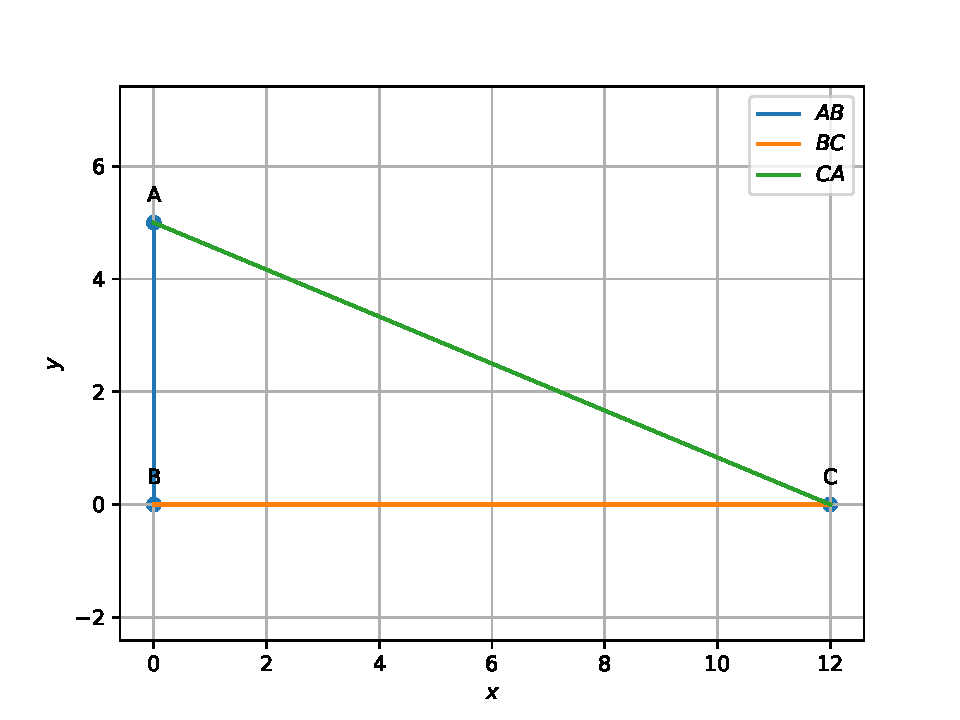
\includegraphics[width=0.75\columnwidth]{chapters/9/11/2/5/figs/vector.pdf}
		\caption{}
		\label{fig:9/11/2/5}
  	\end{figure}

%
\item Construct a triangle $ABC$ in which $\angle{B}=30\degree, \angle{C}=90\degree$ and  $AB+BC+CA=11cm$.
\label{chapters/9/11/2/4}
\\
\solution 
From 
		\eqref{eq:9/11/2/4}
		and
		\eqref{eq:9/11/2/4-final},
		\figref{fig:9/11/2/4}
		is generated.
		See
\begin{lstlisting}
	codes/triangle/const-BCsum.py
\end{lstlisting}
	\begin{figure}[!h]
		\centering
 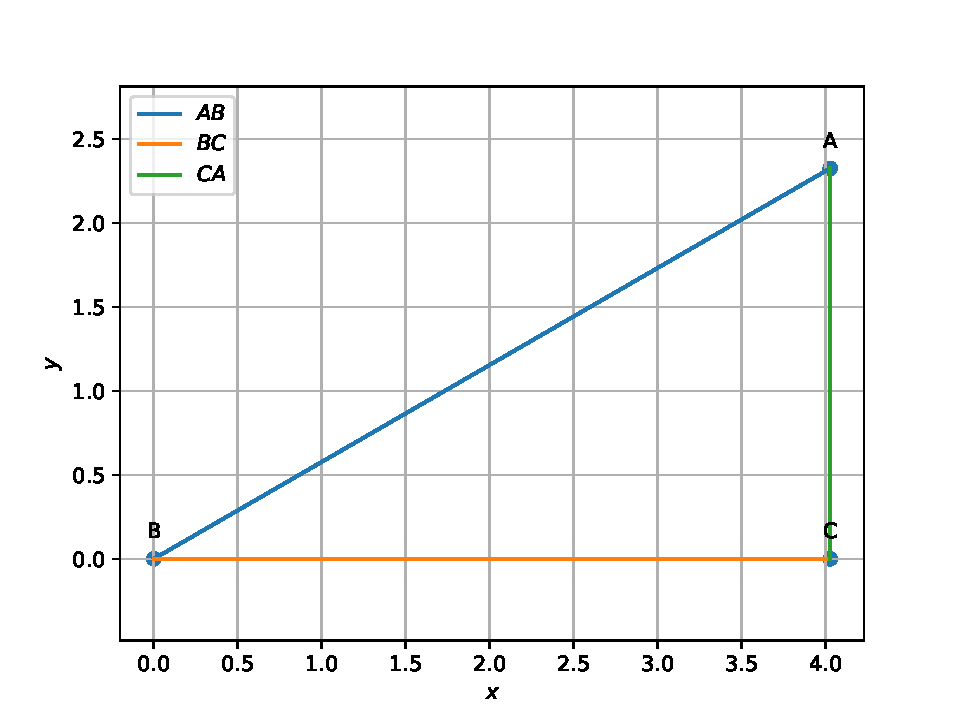
\includegraphics[width=\columnwidth]{chapters/9/11/2/4/figs/vector.pdf}
		\caption{}
		\label{fig:9/11/2/4}
  	\end{figure}

%
\item Draw a right triangle ${ABC}$ in which $BC=12 cm$, $AB=5 cm$ and $\angle{B}=90\degree$.
\item Draw an isosceles triangle ${ABC}$ in which $AB=AC=6cm$ and $BC =6cm$.
\item Draw a triangle ${ABC}$ in which $AB=5cm,BC=6cm$ and $\angle {ABC}=60\degree$.
\item Draw a triangle ${ABC}$ in which $AB=4cm, BC=6cm$ and $AC=9cm$.
\item Draw a triangle ${ABC}$ in which $BC=6 cm, CA=5 cm$ and $AB=4 cm$. 
\item Is it possible to construct a triangle with lengths of its sides as 4$cm$, 3$cm$ and 7$cm$? Give reason for your answer.

\item Is it possible to construct a triangle with lengths of its sides as 9$cm$, 7$cm$ and 17$cm$? Give reason for your answer.

\item Is it possible to construct a triangle with lengths of its sides as 8$cm$, 7$cm$ and 4$cm$? Give reason for your answer.

\item Two sides of a triangle are of lengths 5$cm$ and 1.5$cm$. The length of the third side of the triangle cannot be
\begin{enumerate}
\item $3.6 cm$
\item $4.1 cm$
\item $3.8 cm$
\item $3.4 cm$
\end{enumerate}
\item The construction of a triangle $ABC$, given that $BC = 6 cm, \angle B = 45\degree$ is not possible when difference of $AB$ and $AC$ is equal to
		\begin{enumerate}
			\item 6.9$cm$
			\item 5.2$cm$
			\item 5.0$cm$
			\item 4.0$cm$
		\end{enumerate}
	\item The construction of a triangle $ABC$, given that $BC = 6 cm, \angle C = 60\degree$ is possible when difference of $AB$ and $AC$ is equal to
		\begin{enumerate}
			\item 3.2$cm$
			\item 3.1$cm$
			\item 3$cm$
			\item 2.8$cm$
		\end{enumerate}
\item Construct a triangle whose sides are $3.6 cm$, $3.0 cm$ and $4.8 cm$. Bisect the smallest angle and measure each part.
\item Construct a triangle $ABC$ in which $BC = 5 cm$, $\angle B = 60\degree$ and $AC+AB = 7.5cm$.
\end{enumerate}
Construct each of the following and give justification :
\begin{enumerate}[label=\thesection.\arabic*,ref=\thesection.\theenumi,resume*]
\item A triangle if its perimeter is 10.4$cm$ and two angles are 45\degree and 120\degree.
\item A triangle $PQR$ given that $QR$ = 3$cm$, $\angle PQR = 45\degree$ and $QP - PR = 2 cm$.
\item A right triangle when one side is 3.5$cm$ and sum of other sides and the hypotenuse
is 5.5$cm$.
\item An equilateral triangle if its altitude is 3.2$cm$.
\end{enumerate}                               
Write true or false in each of the following. Give reasons for your answer:
\begin{enumerate}[label=\thesection.\arabic*,ref=\thesection.\theenumi,resume*]
\item A triangle $ABC$ can be constructed in which $AB = 5cm, \angle A =45\degree$ and $BC + AC = 5cm$.
\item A triangle $ABC$ can be constructed in which $BC = 6cm, \angle B =30\degree$ and $AC - AB=4cm$.
\item A triangle $ABC$ can be constructed in which $\angle B =105\degree,\angle C =90\degree$ and $AB + BC + AC = 10cm$.        
\item A triangle $ABC$ can be constructed in which $\angle B =60\degree, \angle C =45 \degree$ and $AB + BC + AC = 12cm$.           
\item Draw a right triangle ${ABC}$ in which $BC=12$ cm, $AB=5$ cm and $\angle{B}=90\degree$.
\item Draw a triangle ${ABC}$ in which $AB$=4 cm, $BC=6 cm\text{ and }AC=9$. 
\item Draw a triangle ${ABC}$ in which $AB$=5 cm. $BC=6 cm\text{ and }\angle {ABC}=60\degree$. 
\item Draw a parallelogram ${ABCD}$ in which $BC=5$ cm, $AB=3$ cm and $\angle{ABC}=60\degree$, divide it into triangles ${ACB}\text{ and }{ABD}$ by the diagonal $BD$. 
Construct the triangle $BD'C'$ similar to $\triangle{BDC}$ with scale factor $\frac{4}{3}$. Draw the line segment $D'A'$ parallel to $DA$ where $\vec{A}$' lies on extended side $BA$. Is $A'BC'D'$ a parallelogram? 
\item Draw a triangle ${ABC}$ in which $BC=6$ cm, $CA=5$ cm and $AB=4$ cm. 
\end{enumerate}

\subsection{CBSE}
\begin{enumerate}[label=\thesubsection.\arabic*,ref=\thesubsection.\theenumi]
    \item Draw a triangle $\triangle ABC$ with $BC = 6 \text{ cm}$, $AB = 5 \text{ cm}$, and $\angle ABC = 60^\circ$. Then construct a triangle whose sides are $\frac{3}{4}$ of the corresponding sides of $\triangle ABC$. \hfill (10, 2018)
\end{enumerate}

\subsection{Quadrilateral}
\begin{enumerate}[label=\thesection.\arabic*,ref=\thesection.\theenumi]
	\item Draw a quadrilateral in the Cartesian plane, whose vertices are (-4, 5), (0, 7), (5, -5) and (-4, -2). 
\item Draw a parallelogram ${ABCD}$ in which $BC=5 cm, AB=3 cm$ and $\angle{ABC}=60\degree$, divide it into triangles ${ACB}\text{ and }{ABD}$ by the diagonal $BD$. 
\item Construct a square of side $3 cm$.
\item Construct  a rectangle whose adjacent sides are of lengths $5 cm$ and $3.5 cm$.
\item Construct a rhombus whose side is of length $3.4 cm$ and one of its angles is $45\degree$.
\item Construct a rhombus whose diagonals are 4 cm and 6 cm in lengths.
\end{enumerate}

\newpage
\section{Linear Forms}
\subsection{Formulae}
\begin{enumerate}[label=\thesubsection.\arabic*.,ref=\thesubsection.\theenumi]
\item The equation of a line is given by 
\begin{align}
			\label{eq:line-school}
	y &= mx + c
	\\
	\implies \myvec{x \\ y} &= \myvec{x \\ 
	 mx + c} =\myvec{0 \\ c} + x\myvec{1 \\ m}
\end{align}
			yielding 
\begin{align}
\label{eq:geo-param}
	\vec{x} = \vec{h} + \kappa \vec{m}.
\end{align}
where $\vec{h}$ is any point on the line and 
\begin{align}
			\label{eq:line-school-dir}
\vec{m} = \myvec{1 \\ m}
\end{align}
is the direction vector. 
\item 
	For
\begin{align}
	\vec{m}^{\top}\vec{n} = 0,
\end{align}
\eqref{eq:geo-param}
	can be expressed as
\begin{align}
	\vec{n}^{\top}\vec{x} &= \vec{n}^{\top}\vec{h} + \kappa \vec{n}^{\top}\vec{m}
	\\
	\begin{split}
	\implies	\vec{n}^{\top}\brak{\vec{x}-\vec{h}} &=0 
	\\
		\text{or, }
	\vec{n}^{\top}\vec{x} &= c
	\end{split}
	\label{eq:geo-normal}
\end{align}
for 
\begin{align}
c = 	\vec{n}^{\top}\vec{h}. 
\end{align}
where
\begin{align}
\vec{n}=\myvec{-m \\ 1}
			\label{eq:line-school-normal}
\end{align}
is defined to be the
{\em normal vector}
		of the line.  
	In 3D, \eqref{eq:geo-normal} represents a plane.
	\iffalse
\item 			\eqref{eq:line-school} can also be expressed as
\begin{align}
	y - mx &= c 
	\\
	\implies \myvec{-m & 1}\myvec{x \\ y} &= c
\end{align}
			yielding 
\begin{align}
	\label{eq:geo-normal}
\vec{n}^{\top}\vec{x} &= c
\end{align}
		\item 
and the normal vector is
\item The equation of a line passing through 
  \item From \eqref{eq:geo-param}, 
	  if $\vec{A},\vec{D}$ and $\vec{C}$ are on the same line,
		\label{prop:lin-dep}
\begin{align}
			\vec{D}=\vec{A}+q\vec{m} 
			\\ 
			\vec{C}=\vec{D}+p\vec{m} \\
			\label{eq:collinear} 
			\implies 	p\brak{\vec{D}-\vec{A}} 
			+ q\brak{\vec{D}-\vec{C}} = 0, \quad p, q \ne 0 \\ 
			\implies \vec{D} = \frac{p\vec{A}+q\vec{C}}{p+q} 
			\end{align} 
			yielding \eqref{eq:section_formula} upon substituting \begin{align} k = \frac{p}{q}. \end{align} 
			$\brak{\vec{D}-\vec{A}}, \brak{\vec{D}-\vec{C}}$ 
		are then said to be {\em linearly dependent}.
			  \fi
	\item If $\vec{A}, \vec{B}, \vec{C}$ are collinear,  from \eqref{eq:geo-normal}, \begin{align}
	 \vec{n}^{\top}\vec{A} &=  c 
	 \\
	 \vec{n}^{\top}\vec{B} &=  c 
	 \\
	 \vec{n}^{\top}\vec{C} &=  c 
\end{align}
which can be expressed as 
\begin{align}
		\label{prop:lin-eq}
	\myvec{ \vec{A} & \vec{B} & \vec{C}}^{\top}\vec{n} = c\myvec{1 \\ 1 \\ 1}
	\\
	\equiv \myvec{ \vec{A} & \vec{B} & \vec{C}}^{\top}\vec{n} = \myvec{1 \\ 1 \\ 1}
		\label{prop:lin-eq-unit-mat},
	\\
	\implies 
	\myvec{ 1 & 1 &1 \\ \vec{A} & \vec{B} & \vec{C}}^{\top}\myvec{\vec{n} \\ -1} &= \vec{0}
		\label{prop:lin-dep-rank}
\end{align}
\iffalse
yielding
		\begin{align}
			\label{eq:line-rank}
			\rank{\myvec{1 & 1 & 1 \\ \vec{A}& \vec{B}&\vec{C}}} = 2
		\end{align}
			  Rank is defined to be the number of linearly indpendent rows or columns of a matrix.
			  \fi
		\item
The equation of a line that does not pass through the origin can be expressed as
\begin{align}
	 \vec{n}^{\top}\vec{x} &=   1
		\label{prop:lin-eq-unit}
\end{align}
\item Let the perpendicular distance from the origin to a line be $p$ and the angle made by the perpendicular with the positive $x$-axis be $\theta$.
	Then 
\begin{align}
	p\myvec{\cos \theta \\ \sin \theta}
\end{align}
is a point on the line as well as the normal vector.
Hence, the equation of the line is 
\begin{align}
	p\myvec{\cos \theta & \sin \theta}
	\cbrak{\vec{x}-p\myvec{\cos \theta \\ \sin \theta}} &= 0
	\\
	\implies 
	\myvec{\cos \theta & \sin \theta}
	\vec{x} &= p
\label{eq:chapters/11/10/2/8-final}
\end{align}
\item Let $\vec{Q}$ be the foot of the perpendicular from $\vec{P}$
	to the line
\begin{align}
			\label{eq:geo-norm-app}
    \vec{n}^{\top}  \vec{x} = c
\end{align}
From
			\eqref{eq:geo-param}
\begin{align}
			\label{eq:geo-param-app}
	\vec{Q} = \vec{P} + k\vec{n}
	\\
	\implies PQ = \norm{\vec{Q} - \vec{P}}=\abs{k} \norm{\vec{n}}
			\label{eq:geo-param-app-PQ}
\end{align}
is the distance from $\vec{Q}$
to the line in 
			\eqref{eq:geo-norm-app}.
			From \eqref{eq:geo-param-app},
\begin{align}
	\vec{n}^{\top}  \vec{Q} = \vec{n}^{\top}  \vec{P} + k\norm{\vec{n}}^2
	\\
	\implies \abs{k} = 
	\frac{\abs{\vec{n}^{\top}\brak{\vec{Q} - \vec{P}}}}{\norm{\vec{n}}^2}
			\label{eq:geo-param-app-k}
			\\
	\implies PQ =\abs{k}  
		\norm{\vec{n}}	=
	\frac{\abs{\vec{n}^{\top}\vec{P} - c}}{\norm{\vec{n}}}
			\label{eq:PQ-final}
\end{align}
upon substituting from 
			\eqref{eq:geo-param-app-PQ}.
\item The foot of the perpendicular is given by
\begin{align}
	\label{eq:11/10/3/4/foot_of_perpendicular}
	\myvec{\vec{m} & \vec{n}}^\top\vec{Q} &= 
	   \myvec{
              \vec{m}^\top\vec{P}\\
	      c
	      }
\end{align}
\item The distance between the parallel lines 
\begin{align}
	\label{eq:parallel_lines}
	\begin{split}
		\vec{n}^{\top}\vec{x} &= c_1
		\\
		\vec{n}^{\top}\vec{x} &= c_2
	\end{split}
\end{align}
is given by 
\begin{align}
	\label{eq:dist_lines_2d}
	d = \frac{\abs{   c_1-c_2 }}{\norm{\vec{n}}}	
\end{align}
	\item 
The reflection of point $\vec{Q}$ w.r.t a line is given by
\begin{align}
	\label{eq:11/10/4/22}
\vec{R} = \vec{Q} -\frac{2\brak{\vec{n}^{\top}\vec{Q}-c}}{\norm{\vec{n}}}\vec{n}
\end{align}
\end{enumerate}

\subsection{Parameters}
Find the direction and normal vectors of each of the following lines
\begin{enumerate}[label=\thesubsection.\arabic*,ref=\thesubsection.\theenumi]
\item $2x+3y=9$
\item $x-\frac{y}{5}-10=10$
\item $-2x+3y=6$
\item $ x=3y$
\item $2x=-5y$
\item $3x+2=0$
\item $y-2=0$
\item $5=2x$
\item $x+y=4$
\item $x-y=2$
\item $y=3x$
\item $3=2x+y$
\item $y=x$
\item $x+y=0$
\item $y=2x$
\item $2+3y=7x$
\item $y=x+2$
\item $y=x-2$
\item $y=-x+2$
\item $x+2y=6$
\item $F=\frac{9}{5}C+32$
\end{enumerate}
Show that two lines $a_1x+b_1y+c_1=0$ and $a_2x+b_2y+c_2=0$ where $b_1b-2\neq 0$ are
\begin{enumerate}[label=\thesubsection.\arabic*,ref=\thesubsection.\theenumi,resume*]
\item parallel if $\frac{a_1}{b_1}=\frac{a_2}{b_2}$ and 
\item Perpendicular if $a_1a_2-b_1b_2=0$.
\end{enumerate}

\subsection{CBSE}
\begin{enumerate}[label=\thesubsection.\arabic*,ref=\thesubsection.\theenumi]
    \item The Cartesian equation of a line $AB$ is
    \begin{align}
        \frac{2x - 1}{12} = \frac{y + 2}{2} = \frac{z - 3}{3}.
    \end{align}
Find the direction cosines of a line parallel to line $AB$.
    \hfill (12, 2023)
    \item Find the direction cosines of a line whose Cartesian equation is given as
    \begin{align}
        3x + 1 = 6y - 2 = 1 - z.
    \end{align}
    \hfill (12, 2022)
\end{enumerate}

\subsection{Equation }
Find the equation of line 
\begin{enumerate}[label=\thesubsection.\arabic*,ref=\thesubsection.\theenumi]
	\item passing through the point $\vec{P} = (– 4, 3)$ with slope $\frac{1}{2}$.
\label{chapters/11/10/2/2}
\\
\solution
Since the normal vector 
\begin{align}
\vec{n}=\myvec{\frac{1}{2}\\ -1}\\
\end{align}
the desired equation \eqref{eq:geo-normal} is 
\begin{align}
\vec{n}^\top \brak{\vec{x}-\vec{P}}&= 0 \\
\implies \myvec{\frac{1}{2}&-1}{\vec{x}}&=-5
\end{align}
See 
		\figref{fig:chapters/11/10/2/2/Figure}.
\begin{figure}[h]
\centering
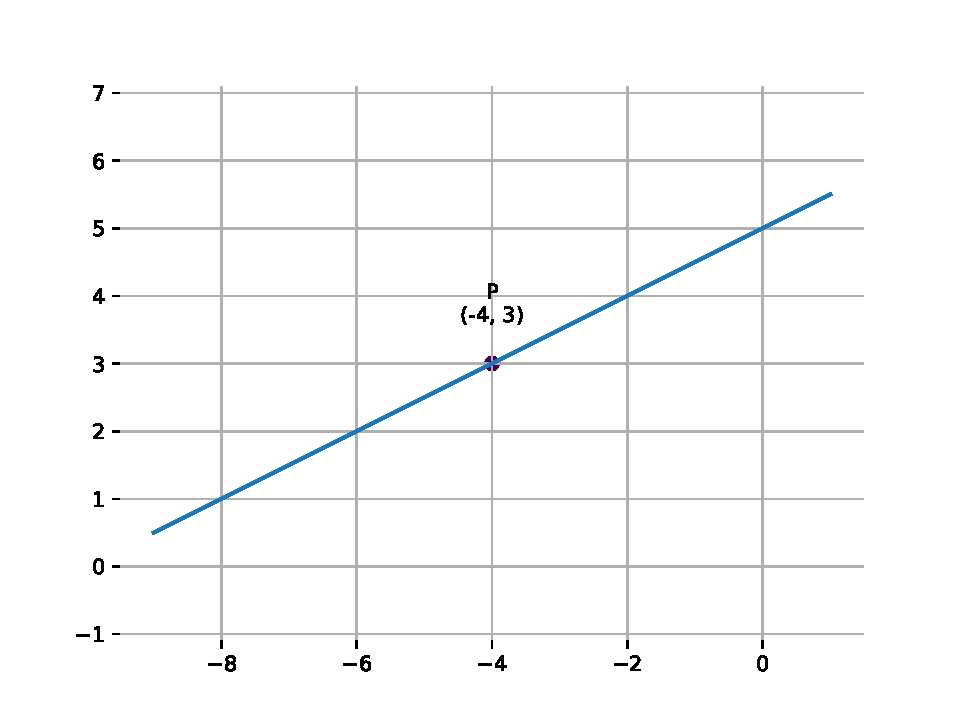
\includegraphics[width=\columnwidth]{chapters/11/10/2/2/figs/fig.pdf}
\caption{}
		\label{fig:chapters/11/10/2/2/Figure}
\end{figure}

	\item passing through $\myvec{0\\0}$ with slope $m$.\\
\label{chapters/11/10/2/3}
\solution
\iffalse
\documentclass[12pt]{article}
\usepackage{graphicx}
%\documentclass[journal,12pt,twocolumn]{IEEEtran}
\usepackage[none]{hyphenat}
\usepackage{graphicx}
\usepackage{listings}
\usepackage[english]{babel}
\usepackage{graphicx}
\usepackage{caption}
\usepackage[parfill]{parskip}
\usepackage{hyperref}
\usepackage{booktabs}
%\usepackage{setspace}\doublespacing\pagestyle{plain}
\def\inputGnumericTable{}
\usepackage{color}                                            %%
    \usepackage{array}                                            %%
    \usepackage{longtable}                                        %%
    \usepackage{calc}                                             %%
    \usepackage{multirow}                                         %%
    \usepackage{hhline}                                           %%
    \usepackage{ifthen}
\usepackage{array}
\usepackage{amsmath}   % for having text in math mode
\usepackage{parallel,enumitem}
\usepackage{listings}
\lstset{
language=tex,
frame=single, 
breaklines=true
}
  
%Following 2 lines were added to remove the blank page at the beginning
\usepackage{atbegshi}% http://ctan.org/pkg/atbegshi
\AtBeginDocument{\AtBeginShipoutNext{\AtBeginShipoutDiscard}}
%
%New macro definitions
\newcommand{\mydet}[1]{\ensuremath{\begin{vmatrix}#1\end{vmatrix}}}
\providecommand{\brak}[1]{\ensuremath{\left(#1\right)}}
\providecommand{\norm}[1]{\left\lVert#1\right\rVert}
\newcommand{\solution}{\noindent \textbf{Solution: }}
\newcommand{\myvec}[1]{\ensuremath{\begin{pmatrix}#1\end{pmatrix}}}
\let\vec\mathbf
\begin{document}
\begin{center}
\title{\textbf{Straight Lines}}
\date{\vspace{-5ex}} %Not to print date automatically
\maketitle
\end{center}
\setcounter{page}{1}
\section*{11$^{th}$ Maths - Chapter 10}
This is Problem-3 from Exercise 10.2
\begin{enumerate}
		\fi
		Line passing through point $\vec{A}=\myvec{0\\0}$ is given by,
\begin{align}
	\vec{n}^\top \brak{\vec{x}-\vec{A}} &= 0\label{eq:11/10/2/31}
\end{align}
Where,
		\begin{align}
			\vec{n} =\myvec{m \\ -1}
		\end{align}
		Substituting $\vec{A}$ and $\vec{n}$ in equation \eqref{eq:11/10/2/31}
		\begin{align}
			\myvec{m & -1}\brak{\vec{x}-\myvec{0\\0}} &=0\\
\implies			\myvec{m & -1}\vec{x} &= 0
		\end{align}
Line segment passing through $\myvec{0\\0}$ with slope $m = 2$ is shown in Fig. \ref{fig:11/10/2/3Fig1}
\begin{figure}[!h]
\begin{center}
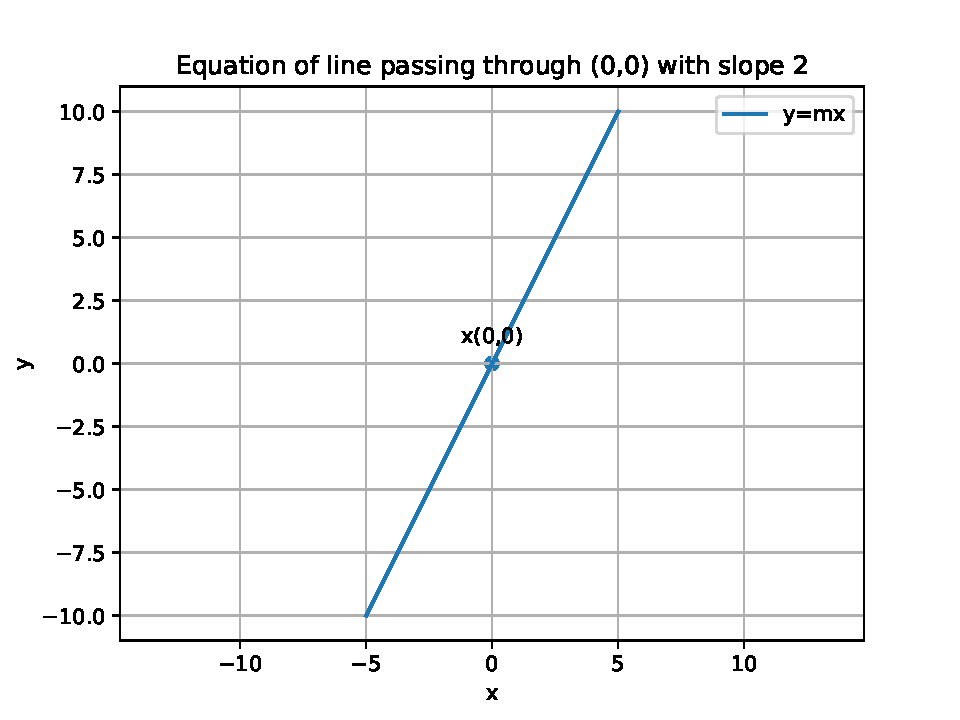
\includegraphics[width=\columnwidth]{chapters/11/10/2/3/figs/fig.pdf}
\end{center}
\caption{}
\label{fig:11/10/2/3Fig1}
\end{figure}

    \item passing through 
    $\vec{A} = \myvec{2\\2\sqrt{3}}$ and inclined with the x-axis at an angle 
    of 75\textdegree.
\label{chapters/11/10/2/4}
\\
    \solution 
    \begin{align}
	    \vec{n} &= \myvec{-1\\2+\sqrt{3}}
        \label{eq:11/10/2/4normal-vec}
	\\
	    \implies
        \implies \vec{n}^\top\vec{x} = \vec{n}^\top\vec{A} &= 4\brak{\sqrt{3}+1} \\
        \implies \myvec{-1&2+\sqrt{3}}\vec{x} &=\myvec{-1&2+\sqrt{3}}\myvec{2\\2\sqrt{3}}  
	    \\
	    &= 4\brak{\sqrt{3}+1}
        \label{eq:11/10/2/4line}
    \end{align}
is the desired equation.  See \figref{fig:11/10/2/4line}.
    \begin{figure}[!ht]
        \centering
        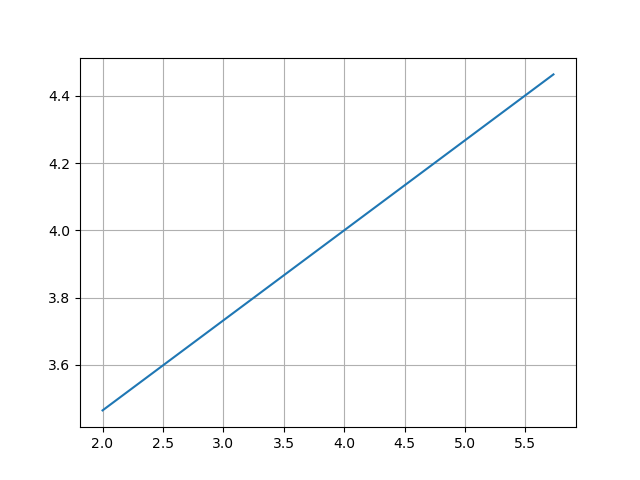
\includegraphics[width=\columnwidth]{chapters/11/10/2/4/figs/line.png}
        \caption{}
        \label{fig:11/10/2/4line}
    \end{figure}

\item intersecting the x-axis at a distance of 3 units to the left of origin with slope of -2.
\label{chapters/11/10/2/5}
\\
\solution 
		From the given information,
\begin{align}		
	\vec{A}=\myvec{-3\\0},\,
\vec{n} = \myvec{2 \\1}.
\end{align}
The desired equation of the line is
\begin{align}
\implies	\myvec { 2 & 1 } \brak{ \vec{x} - \myvec{ -3 \\ 0}} &= 0  \\
	\text{or, }	\myvec{ 2 & 1} \vec{x}  &= -6
        \label{eq:chapters/11/10/2/5/1}
\end{align}
See \figref{fig:chapters/11/10/2/5/Fig1}.
\begin{figure}[H]
	\begin{center}
		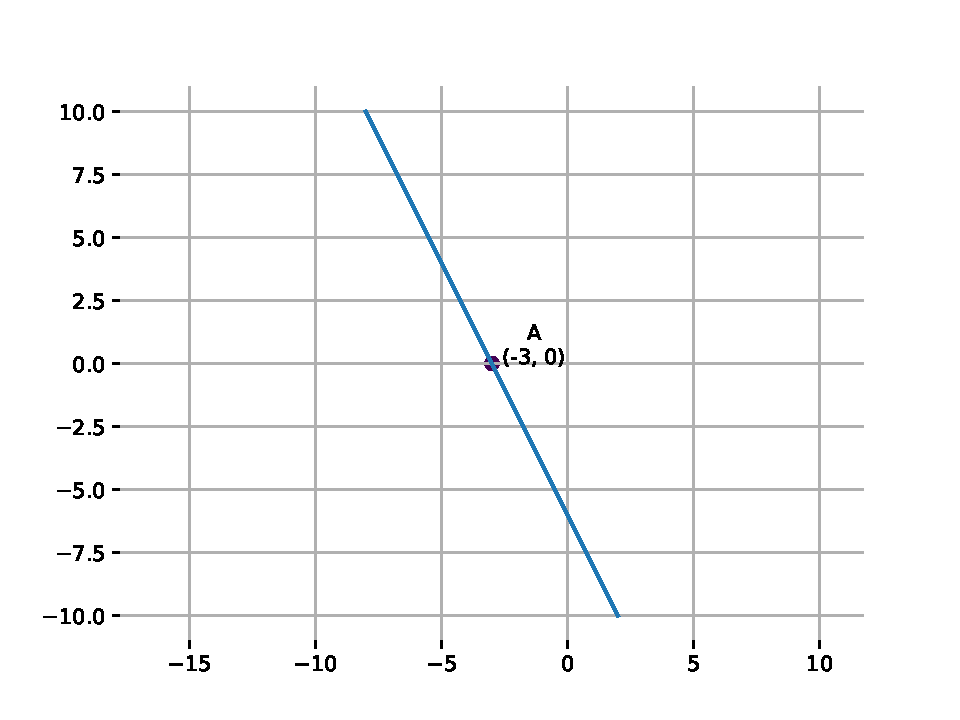
\includegraphics[width=0.75\columnwidth]{chapters/11/10/2/5/figs/fig.pdf}
	\end{center}
\caption{}
\label{fig:chapters/11/10/2/5/Fig1}
\end{figure}


\item intersecting the y-axis at a distance of 2 units above the origin and making an
angle of $30\degree$ with positive direction of the x-axis.
\\
\solution 
\iffalse
\documentclass[journal,12pt,twocolumn]{IEEEtran}
\usepackage{setspace}
\usepackage{gensymb}
\usepackage{xcolor}
\usepackage{caption}
\singlespacing
\usepackage{siunitx}
\usepackage[cmex10]{amsmath}
\usepackage{mathtools}
\usepackage{hyperref}
\usepackage{amsthm}
\usepackage{mathrsfs}
\usepackage{txfonts}
\usepackage{stfloats}
\usepackage{cite}
\usepackage{cases}
\usepackage{subfig}
\usepackage{longtable}
\usepackage{multirow}
\usepackage{enumitem}
\usepackage{bm}
\usepackage{mathtools}
\usepackage{listings}
\usepackage{tikz}
\usetikzlibrary{shapes,arrows,positioning}
\usepackage{circuitikz}
\renewcommand{\vec}[1]{\boldsymbol{\mathbf{#1}}}
\DeclareMathOperator*{\Res}{Res}
\renewcommand\thesection{\arabic{section}}
\renewcommand\thesubsection{\thesection.\arabic{subsection}}
\renewcommand\thesubsubsection{\thesubsection.\arabic{subsubsection}}

\renewcommand\thesectiondis{\arabic{section}}
\renewcommand\thesubsectiondis{\thesectiondis.\arabic{subsection}}
\renewcommand\thesubsubsectiondis{\thesubsectiondis.\arabic{subsubsection}}
\hyphenation{op-tical net-works semi-conduc-tor}

\lstset{
language=Python,
frame=single, 
breaklines=true,
columns=fullflexible
}
\begin{document}
\theoremstyle{definition}
\newtheorem{theorem}{Theorem}[section]
\newtheorem{problem}{Problem}
\newtheorem{proposition}{Proposition}[section]
\newtheorem{lemma}{Lemma}[section]
\newtheorem{corollary}[theorem]{Corollary}
\newtheorem{example}{Example}[section]
\newtheorem{definition}{Definition}[section]
\newcommand{\BEQA}{\begin{eqnarray}}
        \newcommand{\EEQA}{\end{eqnarray}}
\newcommand{\define}{\stackrel{\triangle}{=}}
\newcommand{\myvec}[1]{\ensuremath{\begin{pmatrix}#1\end{pmatrix}}}
\newcommand{\mydet}[1]{\ensuremath{\begin{vmatrix}#1\end{vmatrix}}}
\bibliographystyle{IEEEtran}
\providecommand{\nCr}[2]{\,^{#1}C_{#2}} % nCr
\providecommand{\nPr}[2]{\,^{#1}P_{#2}} % nPr
\providecommand{\mbf}{\mathbf}
\providecommand{\pr}[1]{\ensuremath{\Pr\left(#1\right)}}
\providecommand{\qfunc}[1]{\ensuremath{Q\left(#1\right)}}
\providecommand{\sbrak}[1]{\ensuremath{{}\left[#1\right]}}
\providecommand{\lsbrak}[1]{\ensuremath{{}\left[#1\right.}}
\providecommand{\rsbrak}[1]{\ensuremath{{}\left.#1\right]}}
\providecommand{\brak}[1]{\ensuremath{\left(#1\right)}}
\providecommand{\lbrak}[1]{\ensuremath{\left(#1\right.}}
\providecommand{\rbrak}[1]{\ensuremath{\left.#1\right)}}
\providecommand{\cbrak}[1]{\ensuremath{\left\{#1\right\}}}
\providecommand{\lcbrak}[1]{\ensuremath{\left\{#1\right.}}
\providecommand{\rcbrak}[1]{\ensuremath{\left.#1\right\}}}
\theoremstyle{remark}
\newtheorem{rem}{Remark}
\newcommand{\sgn}{\mathop{\mathrm{sgn}}}
\newcommand{\rect}{\mathop{\mathrm{rect}}}
\newcommand{\sinc}{\mathop{\mathrm{sinc}}}
\providecommand{\abs}[1]{\left\vert#1\right\vert}
\providecommand{\res}[1]{\Res\displaylimits_{#1}}
\providecommand{\norm}[1]{\lVert#1\rVert}
\providecommand{\mtx}[1]{\mathbf{#1}}
\providecommand{\mean}[1]{E\left[ #1 \right]}
\providecommand{\fourier}{\overset{\mathcal{F}}{ \rightleftharpoons}}
\providecommand{\ztrans}{\overset{\mathcal{Z}}{ \rightleftharpoons}}
\providecommand{\system}[1]{\overset{\mathcal{#1}}{ \longleftrightarrow}}
\newcommand{\solution}{\noindent \textbf{Solution: }}
\providecommand{\dec}[2]{\ensuremath{\overset{#1}{\underset{#2}{\gtrless}}}}
\let\StandardTheFigure\thefigure
\def\putbox#1#2#3{\makebox[0in][l]{\makebox[#1][l]{}\raisebox{\baselineskip}[0in][0in]{\raisebox{#2}[0in][0in]{#3}}}}
\def\rightbox#1{\makebox[0in][r]{#1}}
\def\centbox#1{\makebox[0in]{#1}}
\def\topbox#1{\raisebox{-\baselineskip}[0in][0in]{#1}}
\def\midbox#1{\raisebox{-0.5\baselineskip}[0in][0in]{#1}}

\vspace{3cm}
\title{11.10.2.6}
\author{Lokesh Surana}
\maketitle
\section*{Class 11, Chapter 10, Exercise 2.6}


\solution 
\fi
The direction vector of the line is given by
\begin{align}
    \vec{m} = \myvec{1 \\ \tan(30\degree)} = \myvec{1 \\ \frac{1}{\sqrt{3}}}
\end{align}
The normal vector $\vec{n}$ to the line is given by
\begin{align}
    \vec{n} =  \myvec{-\frac{1}{\sqrt{3}} \\ 1}
\end{align}
The line is passing through the point 
\begin{align}
    \vec{A} = \myvec{0 \\ 2}
\end{align}
Hence, 
the equation of the line is given by
\begin{align}
    \vec{n}^\top\brak{\vec{x}-\vec{A}} &= 0 \\
    \implies \myvec{-\frac{1}{\sqrt{3}}&1}\brak{ \vec{x} - \myvec{0 \\ 2}} &= 0  \\
    \text{or, }	\myvec{-\frac{1}{\sqrt{3}}&1} \vec{x}  &= 2
\end{align}
%
\begin{figure}[!htb]
    \centering
    \includegraphics[width=\columnwidth]{chapters/11/10/2/6/figs/line.png}
    \caption{}
    \label{fig:chapters/11/10/2/6/line}
\end{figure}


\item passing through (1,2) and making angle $30\degree$ with $y$-axis.
\item passing through the points $\vec{A}\myvec{-1\\1}$ and $\vec{B}\myvec{2\\-4}$.
\label{chapters/11/10/2/7}
\\
\solution 
\begin{align}
	\vec{m} &= \vec{A} - \vec{B}
= \myvec{-3\\5}
\implies
\vec{n} &= \myvec{5\\3}
\end{align}
Thus, the equation of line is
\begin{align}
 \myvec{ 5 & 3}\vec{x}  &= -2
\end{align}
See 
   \figref{fig:chapters/11/10/2/7/Line_AB}.
\begin{figure}[h!]
  \centering
   \includegraphics[width=\linewidth]{chapters/11/10/2/7/figs/Figure_1.png}
   \caption{}
   \label{fig:chapters/11/10/2/7/Line_AB}
\end{figure}





\item passing through the points $(3,4,-7)$ and $(1,-1,6)$. 
\item The vector equation of the line 
\begin{align*}
	\frac{x-5}{3}=\frac{y+4}{7}=\frac{z-6}{2} 
\end{align*}
is \noindent\rule{2cm}{0.4pt}. 
\item The vector equation of the line 
\begin{align*}
	\frac{x-5}{3}=\frac{y+4}{7}=\frac{z-6}{2}
\end{align*}
 is \noindent\rule{2cm}{0.4pt}.
\item 
The vertices of triangle $PQR$ are $\vec{P}(2,1), \vec{Q}(-2,3), \vec{R}(4,5)$. Find the equation of the median through $\vec{R}$.
\label{chapters/11/10/2/9}
\\
\solution
	\begin{figure}[H]
		\centering
 \includegraphics[width=0.75\columnwidth]{chapters/11/10/2/9/figs/line.png}
		\caption{}
		\label{fig:11/10/2/9}
  	\end{figure}
	See Fig. 
		\ref{fig:11/10/2/9}.
Using section formula, the mid point of $PQ$ is
\begin{align}
\vec{A} = \frac{\vec{P} +\vec{Q} }{2}
	= {\myvec{0\\2}}
\end{align} 
Following the approach in \probref{chapters/11/10/2/7},
\begin{align*}
	\augvec{2}{1}{ 
	4 & 5 & 1
	\\  
	0 & 2 & 1
	}
	\xleftrightarrow[R_2 \leftarrow 4R_2 ]{R_1 \leftarrow 2R_1 -5R_2}
	\augvec{2}{1}{ 
	8 & 0 & -3 
	\\ 
	0 & 8 & 4 
	}
	\implies \vec{n} = \frac{1}{8}\myvec{ -3 \\ 4}
\end{align*}
Thus,
the equation of the line is 
\begin{align}
	\myvec{-3 & 4}\vec{x} =8 
\end{align}

	\item Find the equations of the planes that pass through the points
\begin{enumerate}
\item $\vec{A}= \myvec{1\\1\\– 1}, \vec{B}=\myvec{6\\4\\– 5},\vec{C}= \myvec{– 4\\– 2\\3}$
\item $\vec{A}= \myvec{1\\1\\0}, \vec{B}= \myvec{1\\2\\1}, \vec{C}= \myvec{– 2\\2\\-1}$
\end{enumerate}
    \solution
		\begin{enumerate}
	\item From 
		\eqref{prop:lin-eq-unit-mat},
\begin{align}
\myvec{1&1&-1\\ 6&4&-5\\ -4&-2&3} \vec{n} = \myvec{1\\1\\1}
\end{align}
\begin{align*}
	\implies \myvec{1&1&-1&\vrule&1\\6&4&-5&\vrule&1\\-4&-2&3&\vrule&1}
	\\
\xleftrightarrow[R_3 \leftarrow R_3 + 4R_1]{R_2 \leftarrow R_2 - 6R_1}
\myvec{1&1&-1&\vrule&1\\0&-2&1&\vrule&-5\\0&2&-1&\vrule&5}\\ 
\xleftrightarrow[{R_1 \leftarrow 2R_1 + R_2}] {R_3 \leftarrow R_3 + R_2}
\myvec{2&0&-1&\vrule&-3\\0&2&-1&\vrule&5\\0&0&0&\vrule&0}
\end{align*}
Since we obtain a 0 row, 
the given points are collinear.
The direction vector of the line is
\begin{align}
\vec{m}=\vec{B}-\vec{C} \equiv \myvec{5\\3\\-4}
\end{align}
and the equation of a line is given by,
\begin{align}
	\vec{x}&=\vec{A}+  \kappa\vec{m}\\
&= \myvec{1\\1\\– 1} + \kappa \myvec{5\\3\\-4}
\end{align}
See 
     \figref{fig:chapters/12/11/3/6/1}.
\begin{figure}[h!]
  \centering
   \includegraphics[width=\columnwidth]{chapters/12/11/3/6/figs/collinear_points.png}
    \caption{}
     \label{fig:chapters/12/11/3/6/1}
     \end{figure}
     \item  In this case, 
\begin{align}
\myvec{1&1&0 \\ 1&2&1 \\ -2&2&-1} \vec{n}=\vec{1}
\end{align}
\begin{align*}
\implies
\myvec{1&1&0&\vrule&1\\1&2&1&\vrule&1\\-2&2&-1&\vrule&1}
\\
\xleftrightarrow[R_3 \leftarrow R_3 + 2R_1]{R_2 \leftarrow R_2 - R_1}
\myvec{1&1&0&\vrule&1\\0&1&1&\vrule&0\\0&4&-1&\vrule&3}
\\
	\xleftrightarrow[R_3 \leftarrow R_3 - 4R_2]{R_1 \leftarrow R_1- R_2}
\myvec{1&0&-1&\vrule&1\\0&1&1&\vrule&0\\0&0&-5&\vrule&3}\\
	\xleftrightarrow[R_2 \leftarrow 5R_2 + R_3]{R_1 \leftarrow 5R_1- R_3}
\myvec{5&0&0&\vrule&2\\0&5&0&\vrule&3\\0&0&5&\vrule&-3}
\end{align*}
Hence, the equation of the plane is
\begin{align}
\myvec{2 & 3 & -3} \vec{x} = 5
\end{align}
\end{enumerate}

\item Find the equation of the plane through the points $(2,1,0)$, $(3,-2,-2)$ and $(3,1,7)$.
\item A plane passes through the points $(2,0,0) (0,3,0)$ and $(0,0,4)$. The equation of the plane is \noindent\rule{2cm}{0.4pt}.
\item If the intercept of a line between the coordinate axes is divided by the point (-5,4) in the ratio 1:2 then find the equation of the line.
\item Find the equation of a line that cuts off equal intercepts on the coordinate axes and passes through the point $(2,3)$.  
	\\
\solution 
\label{chapters/11/10/2/12}
Let $(a,0)$  and  $(0,a)$ be the intercept points. 
\begin{align}
\vec{m} 
        &=   \myvec{
		a \\
		0 
		} - \myvec{
		   0 \\
		   a
		}  
        		  \equiv \myvec{
                           1 \\
			   -1 
		         } 
			 \\
			 \implies
\vec{n} &=  \myvec{
		     1 \\
		     1
	     } 
\end{align}
and 
the equation of the  line is
\begin{align}
	\myvec { 1 & 1 } \brak{ \vec{ x  - \myvec{ 2 \\
                                   3
			     }
		}}  &= 0  \\
\implies		\myvec{ 1 & 1} \vec{x}  &= 5 
        \label{eq:11/10/2/12/1}
\end{align}
See  \figref{fig:11/10/2/12/Fig1}.
\begin{figure}[H]
	\begin{center}
		\includegraphics[width=0.75\columnwidth]{chapters/11/10/2/12/figs/problem12.pdf}
	\end{center}
\caption{}
\label{fig:11/10/2/12/Fig1}
\end{figure}


\item 
Find the equation of a line passing through a point (2,2) and cutting off intercepts on the axes whose sum is 9.
\label{chapters/11/10/2/13}
	\\
	\solution 
Let  the intercept points be
\begin{align}
{\vec{P}}=\myvec{
  a\\
  0}
 , {\vec{Q}}=\myvec{
  0\\
  b}
  \text{ and }
   {\vec{R}}=\myvec{
  2\\
  2}
\end{align}
be the given point.  
Forming the collinearity matrix from 
		\eqref{prop:lin-dep-rank},
\begin{align}
	\myvec{ \vec{P}-\vec{Q} &\vec{P}-\vec{R}} 
	=
	 \myvec{
  a & a-2\\
  -b & -2
 }
\end{align}
which is singular if 
\begin{align}
 ab -2\brak{a+b} = 0
 \implies ab = 18
		\label{eq:11/10/2/13-a+b}
		\\
\because  a + b = 9.
\end{align}
$\therefore a,b$
are the roots of
\begin{align}
	x^2 -9x +18 = 0.
\end{align}
yielding
\begin{align}
	\myvec{a \\ b} = \myvec{6 \\ 3}, \myvec{3\\6}
\end{align}
Since 
\begin{align}
	\vec{m} = \myvec{a \\ -b},
	\vec{n} = \myvec{b \\ a} \equiv \myvec{1 \\ 2}, \myvec{2\\1}
\end{align}
Thus, the possible equations of the line are 
\begin{align}
\myvec{1 & 2}\vec{x} = 6
	\\
	\myvec{2&1}\vec{x} = 6
\end{align}
		See \figref{fig:11/10/2/13}.
	\begin{figure}[H]
		\centering
 \includegraphics[width=0.75\columnwidth]{chapters/11/10/2/13/figs/fig.pdf}
		\caption{}
		\label{fig:11/10/2/13}
  	\end{figure}

\item Find the equation of the lines which passes the point (3,4) and cuts off intercepts from the coordinate axes such that their sum is 14.
\item Find the equation of the straight line which passes through the point (1, -2) and cuts off equal intercepts from axes.
\item Find the equation of the line which passes through the point (-4,3) and the portion of the line intercepted between the axes is divided internally in ratio 5:3 by this point.
\item Consider the following population and year graph. Find the slope of the line AB and using it, find what will be the population in the year 2010.
\\
\begin{figure}[H]
\centering
\includegraphics[width=0.75\columnwidth]{chapters/11/10/1/14/figs/fig.png}
\caption{}
\label{fig:chapters/11/10/1/14/1}
\end{figure}
\solution
The direction vector of the line in \figref{fig:chapters/11/10/1/14/1} is
\begin{align}
\vec{m} = \vec{B} - \vec{A}
= \myvec{2 \\ 1}
\\
\implies \vec{n}
= \myvec{1 \\ -2}
\end{align}
 The equation of the line is then given by 
\begin{align}
\vec{n}^{\top} (\vec{x} -\vec{A}) &= 0 \\
\implies 
\myvec{1& -2} \vec{x} &= 1801
\\
\implies  \myvec{1&-2} \myvec{2010\\y} &= 1801 \\
\implies y &= \frac{209}{2}
\end{align}





\item Slope of a line which cuts off intercepts of equal length on the axes is 
\begin{enumerate}
\item -1
\item -0
\item 2
\item $\sqrt{3}$
\end{enumerate}
\item If the coordinates of middle point of the portion of a line intercepted between the coordinate axes is (3,2),then the equation of the line will be
\begin{enumerate}
\item $2x+3y=12$
\item $3x+2y=12$
\item $4x-3y=6$
\item $5x-2y=10$
\end{enumerate}
\item If the line $\frac{x}{a}+\frac{y}{b}=1$ passes the points (2,-3) and (4,-5), then $(a,b)$ is 
\begin{enumerate}
\item (1,1)
\item (-1,1)
\item (1,-1)
\item (-1,-1)
\end{enumerate}
\item The intercepts made by the plane $2x-3y+5z+4=0$ on the co-ordinate axis are $\brak{-2,\frac{4}{3},-\frac{4}{5}}$.
\item The line $\overrightarrow{r}=2\hat{i}-3\hat{j}-\hat{k}+\lambda(\hat{i}-\hat{j}+2\hat{k})$ lies in the plane $\overrightarrow{r} \cdot (3\hat{i}+\hat{j}-\hat{k})+2=0$.
\end{enumerate}

\subsection{CBSE}
\begin{enumerate}[label=\thesubsection.\arabic*, ref=\thesubsection.\theenumi]
\item Show that the plane $x - 5y - 2z = 1$ contains the line $\frac{x - 5}{3}$ = y = $2 -z$.
\hfill (12, 2020)
    \item If the equation of a line is
    \begin{align}
        x &= ay + b, \\
        z &= cy + d,
    \end{align}
    then find its parametric form
    \hfill (12, 2023)
    \item Equation of the line passing through the origin and making $30\degree$, $60\degree$, and $90\degree$ with the $x, y, z$ axes respectively is
    \hfill (12, 2023)
	\item A line passes through the point with position vector $2\hat{i} - \hat{j} + 4\hat{k}$ and is in the direction of the vector $\hat{i} + \hat{j} - 2\hat{k}$. Find the equation of the line in Cartesian form. \hfill (12, 2019)
	\item Find the vector and Cartesian equations of the plane passing through the points having position vectors $\hat{i} + \hat{j} - 2\hat{k}$, $2\hat{i} - \hat{j} + \hat{k}$, and $\hat{i} + 2\hat{j} + \hat{k}$. (12, 2019)
	\item Find the Cartesian and vector equations of the plane passing through the points $A(2, 5, -3)$, $B(-2, -3, 5)$, and $C(5, 3, -3)$. \hfill (12, 2019)
	\item Write the equation of a plane passing through the point $(2, 3, 7)$ and parallel to the plane obtained above. Hence, find the distance between the two parallel planes. \hfill (12, 2019)
	\item Find the vector equation of a line passing through the point $(2, 3, 2)$ and parallel to the line $\overrightarrow{r} = (-2\hat{i} + 3\hat{j}) + \lambda (2\hat{i} - 3\hat{j} + 6\hat{k})$. Also, find the distance between these two lines. \hfill (12, 2019)
	\item Find the value of $\vec{x}$ such that the four points with position vectors $\vec{A}(3\hat{i} + 2\hat{j} + \hat{k})$, $\vec{B}(4\hat{i} + x\hat{j} + 5\hat{k})$, $\vec{C}(4\hat{i} + 2\hat{j} - 2\hat{k})$, and $\vec{D}(6\hat{i} + 5\hat{j} - \hat{k})$ are coplanar. \hfill (12, 2019)
	\item Using vectors, find the value of $\vec{x}$ such that the four points $A(x, 5, -1)$, $B(3, 2, 1)$, $C(4, 5, 5)$, and $D(4, 2, -2)$ are coplanar. \hfill (12, 2019)
\item Find the value of $a$ so that the point $(3, a)$ lies on the line represented by $2x - 3y = 5$. \hfill (10, 2019)
\item Point $P$ divides the line segment joining the points $A(2, 1)$ and $B(5, -8)$ such that $\frac{AP}{AB} = \frac{1}{3}$. If $P$ lies on the line $2x - y + k = 0$, find the value of $k$. \hfill (10, 2019)
\item The line segment joining the points $A(2, 1)$ and $B(5, -8)$ is trisected at the points $P$ and $Q$ such that $P$ is nearer to $A$. If $P$ also lies on the line given by $2x - y + k = 0$, find the value of $k$. \hfill (10, 2019)
    \item The line segment joining the points $\vec{A}(2,1)$ and $\vec{B}(5,-8)$ is trisected at the points $\vec{P}$ and $\vec{Q}$, where $\vec{P}$ is nearer to $\vec{A}$. If $\vec{P}$ lies on the line $2x - y + k = 0$, find the value of $k$. \hfill (10, 2018)
\item Find the vector and cartesian equations of the plane passing through the points $\brak{2,5,-3},\brak{-2,-3,5}$ and $\brak{5,3,-3}$. also find the point of intersection of this plane with the line passing through points $\brak{3,1,5}$ and $\brak{-1,-3,-1}$.
\hfill (12, 2018)
\item A line passes through the point with position vector $2\hat{i}-\hat{j}+4\hat{k}$ and is in the direction of the vector $\hat{i}+\hat{j}-2\hat{k}$. Find the equation of the line in cartesian form.
\hfill (12, 2018) 
\item Find the cartesian and vector equations of the plane passing through the points $A$ $\brak{2, 5, -3}$, $B$ $\brak{-2, -3, 5}$, and $C$ $\brak{5, 3, -3}$.

\hfill (12, 2018) 
\end{enumerate}

\subsection{Parallel}
\begin{enumerate}[label=\thesubsection.\arabic*, ref=\thesubsection.\theenumi]
	\item  Find the vector equation of the line passing through $\myvec{1&2&3}^{\top}$ and parallel to the planes $\myvec{1&-1&2}\vec{x} = 5$ and $\myvec{3&1&1}\vec{x} = 6$.  
		\\
    \solution
		The direction vector of the line  is given by 
\begin{align*}
 \myvec{1&-1&2 \\ 3&1&1}\vec{m} = 0
 \xleftrightarrow[]{R_2\rightarrow -\frac{3}{4}{R_1} + \frac{1}{4}{R_2}} \myvec{1&-1&2 \\ 0&1&-\frac{5}{4}}\\
   \myvec{1&-1&2 \\ 0&1&-\frac{5}{4}} \xleftrightarrow[]{R_1\rightarrow {R_1} + {R_2}} \myvec{1&0&\frac{3}{4} \\ 0&1&-\frac{5}{4}}
   \\
 \implies \vec{m} =\myvec{-3\\5\\4}
\end{align*}
$\therefore$ the equation of the line is
\begin{align}
    \vec{x} = \myvec{1\\2\\3} + \lambda\myvec{-3\\5\\4} 
\end{align}


	\item Find the equation of the plane with an intercept 3 on the Y-axis and parallel to ZOX-Plane.\\
    \solution
		\iffalse
\documentclass[A4,12pt,twocolumn]{IEEEtran}
%
\usepackage{setspace}
\usepackage{gensymb}
%\doublespacing
\singlespacing

%\usepackage{graphicx}
%\usepackage{amssymb}
%\usepackage{relsize}
\usepackage[cmex10]{amsmath}
%\usepackage{amsthm}
%\interdisplaylinepenalty=2500
%\savesymbol{iint}
%\usepackage{txfonts}
%\restoresymbol{TXF}{iint}
%\usepackage{wasysym}
\usepackage{amsthm}
%\usepackage{iithtlc}
\usepackage{mathrsfs}
\usepackage{txfonts}
\usepackage{stfloats}
\usepackage{bm}
\usepackage{cite}
\usepackage{cases}
\usepackage{subfig}
%\usepackage{xtab}
\usepackage{longtable}
\usepackage{multirow}
%\usepackage{algorithm}
%\usepackage{algpseudocode}
\usepackage{enumitem}
\usepackage{mathtools}
\usepackage{steinmetz}
\usepackage{tikz}
\usepackage{circuitikz}
\usepackage{verbatim}
\usepackage{tfrupee}
\usepackage[breaklinks=true]{hyperref}
%\usepackage{stmaryrd}
\usepackage{tkz-euclide} % loads  TikZ and tkz-base
%\usetkzobj{all}
\usetikzlibrary{calc,math}
\usepackage{listings}
    \usepackage{color}                                            %%
    \usepackage{array}                                            %%
    \usepackage{longtable}                                        %%
    \usepackage{calc}                                             %%
    \usepackage{multirow}                                         %%
    \usepackage{hhline}                                           %%
    \usepackage{ifthen}                                           %%
  %optionally (for landscape tables embedded in another document): %%
    \usepackage{lscape}     
\usepackage{multicol}
\usepackage{chngcntr}
%\usepackage{enumerate}

%\usepackage{wasysym}
%\newcounter{MYtempeqncnt}
\DeclareMathOperator*{\Res}{Res}
%\renewcommand{\baselinestretch}{2}
\renewcommand\thesection{\arabic{section}}
\renewcommand\thesubsection{\thesection.\arabic{subsection}}
\renewcommand\thesubsubsection{\thesubsection.\arabic{subsubsection}}

\renewcommand\thesectiondis{\arabic{section}}
\renewcommand\thesubsectiondis{\thesectiondis.\arabic{subsection}}
\renewcommand\thesubsubsectiondis{\thesubsectiondis.\arabic{subsubsection}}

% correct bad hyphenation here
\hyphenation{op-tical net-works semi-conduc-tor}
\def\inputGnumericTable{}                                 %%

\lstset{
%language=C,
frame=single, 
breaklines=true,
columns=fullflexible
}
%\lstset{
%language=tex,
%frame=single, 
%breaklines=true
%}

\begin{document}
%


\newtheorem{theorem}{Theorem}[section]
\newtheorem{problem}{Problem}
\newtheorem{proposition}{Proposition}[section]
\newtheorem{lemma}{Lemma}[section]
\newtheorem{corollary}[theorem]{Corollary}
\newtheorem{example}{Example}[section]
\newtheorem{definition}[problem]{Definition}
%\newtheorem{thm}{Theorem}[section] 
%\newtheorem{defn}[thm]{Definition}
%\newtheorem{algorithm}{Algorithm}[section]
%\newtheorem{cor}{Corollary}
\newcommand{\BEQA}{\begin{eqnarray}}
\newcommand{\EEQA}{\end{eqnarray}}
\newcommand{\define}{\stackrel{\triangle}{=}}

\bibliographystyle{IEEEtran}
%\bibliographystyle{ieeetr}


\providecommand{\mbf}{\mathbf}
\providecommand{\pr}[1]{\ensuremath{\Pr\left(#1\right)}}
\providecommand{\qfunc}[1]{\ensuremath{Q\left(#1\right)}}
\providecommand{\sbrak}[1]{\ensuremath{{}\left[#1\right]}}
\providecommand{\lsbrak}[1]{\ensuremath{{}\left[#1\right.}}
\providecommand{\rsbrak}[1]{\ensuremath{{}\left.#1\right]}}
\providecommand{\brak}[1]{\ensuremath{\left(#1\right)}}
\providecommand{\lbrak}[1]{\ensuremath{\left(#1\right.}}
\providecommand{\rbrak}[1]{\ensuremath{\left.#1\right)}}
\providecommand{\cbrak}[1]{\ensuremath{\left\{#1\right\}}}
\providecommand{\lcbrak}[1]{\ensuremath{\left\{#1\right.}}
\providecommand{\rcbrak}[1]{\ensuremath{\left.#1\right\}}}
\theoremstyle{remark}
\newtheorem{rem}{Remark}
\newcommand{\sgn}{\mathop{\mathrm{sgn}}}
\providecommand{\abs}[1]{\left\vert#1\right\vert}
\providecommand{\res}[1]{\Res\displaylimits_{#1}} 
\providecommand{\norm}[1]{\left\lVert#1\right\rVert}
%\providecommand{\norm}[1]{\lVert#1\rVert}
\providecommand{\mtx}[1]{\mathbf{#1}}
\providecommand{\mean}[1]{E\left[ #1 \right]}
\providecommand{\fourier}{\overset{\mathcal{F}}{ \rightleftharpoons}}
%\providecommand{\hilbert}{\overset{\mathcal{H}}{ \rightleftharpoons}}
\providecommand{\system}{\overset{\mathcal{H}}{ \longleftrightarrow}}
	%\newcommand{\solution}[2]{\textbf{Solution:}{#1}}
\newcommand{\solution}{\noindent \textbf{Solution: }}
\newcommand{\cosec}{\,\text{cosec}\,}
\providecommand{\dec}[2]{\ensuremath{\overset{#1}{\underset{#2}{\gtrless}}}}
\newcommand{\myvec}[1]{\ensuremath{\begin{pmatrix}#1\end{pmatrix}}}
\newcommand{\mydet}[1]{\ensuremath{\begin{vmatrix}#1\end{vmatrix}}}
%\numberwithin{equation}{section}
\numberwithin{equation}{subsection}
%\numberwithin{problem}{section}
%\numberwithin{definition}{section}
\makeatletter
\@addtoreset{figure}{problem}
\makeatother

\let\StandardTheFigure\thefigure
\let\vec\mathbf
%\renewcommand{\thefigure}{\theproblem.\arabic{figure}}
\renewcommand{\thefigure}{\theproblem}
%\setlist[enumerate,1]{before=\renewcommand\theequation{\theenumi.\arabic{equation}}
%\counterwithin{equation}{enumi}


%\renewcommand{\theequation}{\arabic{subsection}.\arabic{equation}}

\def\putbox#1#2#3{\makebox[0in][l]{\makebox[#1][l]{}\raisebox{\baselineskip}[0in][0in]{\raisebox{#2}[0in][0in]{#3}}}}
     \def\rightbox#1{\makebox[0in][r]{#1}}
     \def\centbox#1{\makebox[0in]{#1}}
     \def\topbox#1{\raisebox{-\baselineskip}[0in][0in]{#1}}
     \def\midbox#1{\raisebox{-0.5\baselineskip}[0in][0in]{#1}}

\vspace{3cm}


\title{GEOMETRY}
\author{Shristy Sharma (EE22BNITS11001)}





% make the title area
\maketitle

\newpage

%\tableofcontents

\bigskip

\renewcommand{\thefigure}{\theenumi}
\renewcommand{\thetable}{\theenumi}
%\renewcommand{\theequation}{\theenumi}


%Download all python codes 
%
%\begin{lstlisting}
%svn co https://github.com/JayatiD93/trunk/My_solution_design/codes
%\end{lstlisting}

%Download all and latex-tikz codes from 
%
%\begin{lstlisting}
%svn co https://github.com/gadepall/school/trunk/ncert/geometry/figs
%\end{lstlisting}
%


\section{PROBLEM 1}
SOLUTION:\\
\fi
The normal vector to the ZOX plane is
\begin{align} 
\vec{n} = \myvec{0\\1\\0}.
\end{align}
Since, Y-axis has the intercept 3, the desired plane passes through the point
\begin{align}
\vec{P}=\myvec{0\\3\\0}.
\end{align}
Thus, the equation of the plane is given by,
\begin{align}
	\vec{n}^\top \brak{\vec{x}-\vec{P}} &= 0\\
	\implies \myvec{0&1&0} \vec{x}&= 3
\end{align}
See Fig. 
     \ref{fig:chapters/12/11/3/8/1}.
\begin{figure}[h!]
  \centering
   \includegraphics[width=\columnwidth]{chapters/12/11/3/8/figs/plane1.png}
    \caption{}
     \label{fig:chapters/12/11/3/8/1}
     \end{figure}  

\item Find the equation of the line  parallel to the line $3x-4y+2=0$ and passing through the point (-2, 3).
\label{chapters/11/10/3/7}
\\
\solution 
\iffalse
% #######################################
% ########### FILL THESE IN #############
% #######################################
\def\mytitle{MATRICES}
\def\mykeywords{}
\def\myauthor{GOWTHAMI MANDAVA}
\def\contact{gowthamimandava999@gmail.com}
\def\mymodule{ Future Wireless Communication(FWC22012)}
% #######################################
% #### YOU DON'T NEED TO TOUCH BELOW ####
% #######################################
\newcommand{\myvec}[1]{\ensuremath{\begin{pmatrix}#1\end{pmatrix}}}
\let\vec\mathbf
\providecommand{\pr}[1]{\ensuremath{\Pr\left(#1\right)}}
\providecommand{\qfunc}[1]{\ensuremath{Q\left(#1\right)}}
\providecommand{\sbrak}[1]{\ensuremath{{}\left[#1\right]}}
\providecommand{\lsbrak}[1]{\ensuremath{{}\left[#1\right.}}
\providecommand{\rsbrak}[1]{\ensuremath{{}\left.#1\right]}}
\providecommand{\brak}[1]{\ensuremath{\left(#1\right)}}
\providecommand{\lbrak}[1]{\ensuremath{\left(#1\right.}}
\providecommand{\rbrak}[1]{\ensuremath{\left.#1\right)}}
\providecommand{\cbrak}[1]{\ensuremath{\left\{#1\right\}}}
\providecommand{\lcbrak}[1]{\ensuremath{\left\{#1\right.}}
\providecommand{\rcbrak}[1]{\ensuremath{\left.#1\right\}}}
\documentclass[10pt, a4paper]{article}
\usepackage[a4paper,outer=1.5cm,inner=1.5cm,top=1.75cm,bottom=1.5cm]{geometry}
\twocolumn
\usepackage{circuitikz}
\usepackage{amsmath,bm}
\usepackage{amsthm}
\usepackage{mathtools}
\usepackage{amsfonts}
\usepackage{amssymb}
\usepackage{graphicx}
\graphicspath{{./images/}}
%colour our links, remove weird boxes
\usepackage[colorlinks,linkcolor={black},citecolor={blue!80!black},urlcolor={blue!80!black}]{hyperref}
%Stop indentation on new paragraphs
\usepackage[parfill]{parskip}
%% Arial-like font
\usepackage{lmodern}
\renewcommand*\familydefault{\sfdefault}
%Napier logo top right
\usepackage{watermark}
%Lorem Ipusm dolor please don't leave any in you final report ;)
\usepackage{karnaugh-map} 
\usepackage{tabularx}
\usepackage{lipsum}
\usepackage{xcolor}
\usepackage{listings}
%give us the Capital H that we all know and love
\usepackage{float}
%tone down the line spacing after section titles
\usepackage{titlesec}
%Cool maths printing
\usepackage{amsmath}
%PseudoCode
\usepackage{algorithm2e}

\titlespacing{\subsection}{0pt}{\parskip}{-3pt}
\titlespacing{\subsubsection}{0pt}{\parskip}{-\parskip}
\titlespacing{\paragraph}{0pt}{\parskip}{\parskip}
\newcommand{\figuremacro}[5]{
    \begin{figure}[#1]
        \centering
        \includegraphics[width=#5\columnwidth]{#2}
        \caption[#3]{\textbf{#3}#4}
        \label{fig:#2}
    \end{figure}
}


 \lstset{
frame=single, 
breaklines=true,
columns=fullflexible
}

\thiswatermark{\centering \put(1,-110){\includegraphics[scale=0.05]{IIT_logo.jpg}} }
\title{\mytitle}
\author{\myauthor\hspace{1em}\\\contact\\IITH\hspace{0.5em}-\hspace{0.5em}\mymodule}
\date{}
\hypersetup{pdfauthor=\myauthor,pdftitle=\mytitle,pdfkeywords=\mykeywords}
\sloppy
% #######################################
% ########### START FROM HERE ###########
% #######################################
\begin{document}
 \maketitle
 \tableofcontents
 
    
 

 
    
    
    
 
 \Large\section{Problem}
 \fi
\\
\solution 
\iffalse
 \section{Solution}
 \begin{center}
 Given equation is 3x-4y+2=0
\\the parallel line passing through point(-2,3)
\begin{align}
\textbf{n}^{\top}(\textbf{x}-\textbf{p})=0 
\end{align}
\label{tab:truthtable}
    \setlength{\arrayrulewidth}{0.2mm}
\setlength{\tabcolsep}{5pt}
\renewcommand{\arraystretch}{1.25}
    \begin{tabular}{|c|c|}
    \hline % <-- Alignments: 1st column left, 2nd middle and 3rd right, with vertical lines in between
      \large\textbf{Symbol} & \large\textbf{Co-ordinates} \\
      \hline
       \large \textbf{n} & $\ \begin{pmatrix} 3\\ -4 \end{pmatrix}$  \\
       \hline
       \large p & $\ \begin{pmatrix} -2\\ 3 \end{pmatrix}$ \\
       \hline
       	\large c & 2 \\
      \hline
   \end{tabular}
\\ by substituting we get
\fi
From the given information, 
\begin{align}
{\vec{n}}=\myvec{3\\-4} \\
\implies 
	\myvec{3&-4}\cbrak{\vec{x}-\myvec{-2\\3}}&=0
	\\
	&=-18 
\end{align}
which is the required equation of the line.
\iffalse
  therefore,the equation parallel to the given equation and passing through the point(-2,3) is 3x-4y+18=0
 \end{center}
 \section{Plot}
         \centering
        \includegraphics[scale=0.275]{mat.jpg}
  \section{Software}
  We can get the parallel equation of given equation and the plot of two equtions by executing the following code:
 \vspace{3mm} 
\begin{lstlisting}

https://github.com/Gowt-hami/fwc-1-module1/blob/main/par.py
\end{lstlisting}
\end{document}
\fi

\item 
	Find the equation of the line through the point (0, 2) making an angle $\frac{2\pi}{3}$ with the positive X-axis. Also find the equation of the line parallel to it and crossing the Y-axis at a distance of 2 units below the origin.
	\\
	\solution
\label{chapters/11/10/2/14}
The equation of the first line is 
\begin{align}
	\myvec{\sqrt{3} &1}\myvec{\vec{x}-\myvec{0\\2}}&=0
	\\
	\implies 
	\myvec{\sqrt{3}&1}
	\vec{x}&=2
\end{align}
The equation of the second line is 
\begin{align}
	\myvec{\sqrt{3} &1}\myvec{\vec{x}-\myvec{0\\-2}}&=0
	\\
	\implies 
	\myvec{\sqrt{3}&1}
\vec{x}=-2
\end{align}
See
		\figref{fig:11/10/2/14}.
	\begin{figure}[!ht]
		\centering
 \includegraphics[width=\columnwidth]{chapters/11/10/2/14/figs/fig.pdf}
		\caption{}
		\label{fig:11/10/2/14}
  	\end{figure}

\item  Find the vector equation of the line which is parallel to the vector $3\hat{i}-2\hat{j}+6\hat{k}$ and passes through the point $(1, -2, 3)$.
\item Find the equations of the line passing through the point $(3, 0, 1)$ and parallel to the planes $x+2y=0$ and $3y-z=0.$
\item The equation of a line,  which is parallel to $2\hat{i}+\hat{j}+3\hat{k}$ and passes through the point $(5, -2, 4)$ is $\dfrac{x-5}{2}=\dfrac{y+2}{-1}=\dfrac{z-4}{3}$.
\item The value of $\lambda$ for which the vectors $3\hat{i}-6\hat{j}+\hat{k}$ $\text{and}$,   $2\hat{i}-4\hat{j}$+$\lambda\hat{k}$ are parallel is
	\begin{enumerate}
			\setlength{\itemsep}{1ex}
\item $\frac{2}{3}$
\item $\frac{3}{2}$
\item $\frac{5}{2}$
\item $\frac{2}{5}$
	\end{enumerate}	
\item Equation of the line passing through (1, 2) and parallel to the line $y=3x-1$ is
\begin{enumerate}
\item $y+2=x+1$
\item $y+2=3(x+1)$
\item $y-2=3(x-1)$
\item $y-2=x-1$
\end{enumerate}
\item  Find the equation of the line which passes through the point $(1, 2, 3)$ and is parallel to the vector $3\hat{i}+2\hat{j}-2\hat{k}$
\item Find the cartesian equation of the line which passes through the point $(-2, 4, -5)$ and parallel to the line given by $ \frac{x+3}{3}=\frac{y-4}{5}=\frac{z+8}{6}$.
\item Find the equation of the plane passing through $(a, b, c)$ and parallel to the plane $\overrightarrow{r} \cdot (\hat{i}+\hat{j}+\hat{k})=2$.
\item Find the equations of the lines parallel to axes and passing through $(2,3)$.
\item Find the equation of the line through the point $(5, 2, -4)$ and which is parallel to the vector $3 \hat{i}+2 \hat{j}- 8 \hat{k}$.
\end{enumerate}

\subsection{Perpendicular}
\begin{enumerate}[label=\thesubsection.\arabic*,ref=\thesubsection.\theenumi]
	\item Find the values of $\theta \text{ and } p$, if the equation $x\cos\theta+y\sin\theta=p$ is the normal form
of the line $\sqrt{3}x+y+2=0$.
\\
\solution
				\begin{align}
	\vec{n}=\myvec{\sqrt{3}\\1},
			c=-2
			\\
			\implies
			\theta=\tan^{-1}\brak{\sqrt{3}}
			=\frac{\pi}{3},
			p=\frac{\abs{c}}{\norm{\vec{n}}}=1
		\end{align}
See \figref{fig:chapters/11/10/4/2/Fig1}.
\begin{figure}[H]
	\begin{center} 
	    \includegraphics[width=0.75\columnwidth]{chapters/11/10/4/2/figs/line.png}
	\end{center}
\caption{}
\label{fig:chapters/11/10/4/2/Fig1}
\end{figure}


\item  Reduce the following equations into normal form. Find their perpendicular distances from the origin and angle between perpendicular and the positive $x$-axis.
\label{chapters/11/10/3/3}
\begin{enumerate}
	\item $x-\sqrt{3}y+8=0$ 
	\item $y-2=0$
	\item $x-y=4$
\end{enumerate}
\solution
\iffalse
\documentclass[12pt]{article}
\usepackage{graphicx}
\usepackage{amsmath}
\usepackage{mathtools}
\usepackage{gensymb}
\usepackage[utf8]{inputenc}
\usepackage{float}
\newcommand{\mydet}[1]{\ensuremath{\begin{vmatrix}#1\end{vmatrix}}}
\providecommand{\brak}[1]{\ensuremath{\left(#1\right)}}
\providecommand{\norm}[1]{\left\lVert#1\right\rVert}
\newcommand{\solution}{\noindent \textbf{Solution: }}
\newcommand{\myvec}[1]{\ensuremath{\begin{pmatrix}#1\end{pmatrix}}}
\let\vec\mathbf

\begin{document}
\begin{center}
\textbf\large{CLASS-11 \\ CHAPTER-10 \\ STRAIGHT LINES}
\end{center}
\section*{Excercise 10.3}

\solution
\fi
\begin{enumerate}
\item The given equation can be expressed as
		\begin{align}
			\myvec{ 1 & -\sqrt{3}}\vec{x}= -8
			\end{align}
			yielding
\begin{align}
			\vec{n} = \myvec{ 1 & -\sqrt{3}}, c = -8
\end{align}
From the above, the	angle between perpendicular and the positive $x$-axis is given by
		\begin{align}
			\tan^{-1}\brak{-\sqrt{3}} = \frac{2\pi}{3}
		\end{align}
	The perpendicular distance from the origin to the line is given by
		\begin{align}
			d=\frac{\abs{c}}{\norm{\vec{n}}}=4
		\end{align}
\item In this case, the given equation becomes
          \begin{align}
		  \myvec{0 & 1}\vec{x} = 2
          \end{align}
	  yielding
                  \begin{align}
			  \vec{n}=\myvec{0\\1}, c = 2
                          \end{align}
          Angle between perpendicular and the positive $x$-axis is given by:
		\begin{align}  
			\tan^{-1}\infty = \frac{\pi}{2}
                \end{align}      
and  the perpendicular distance from the origin to the line is given by    
                                      \begin{align}
					      d=\frac{|c|}{\norm{\vec{n}}}=2             
                  \end{align}
\item   The given equation can be expressed as
                  \begin{align}
      \myvec{-1 & 1}\vec{x} = 4
                          \end{align}
			  yielding
                  \begin{align}
			  \vec{n}=\myvec{1\\-1}, c = 4
                          \end{align}
          Angle between perpendicular and the positive $x$-axis is given by
		\begin{align}   
			\tan^{-1}\brak{-1} = \frac{3\pi}{4}
                \end{align}                                                                           The perpendicular distance from the origin to the line is given by
		\begin{align}
			d=\frac{|c|}{\norm{\vec{n}}}=\frac{4}{\sqrt{2}}=2\sqrt{2}                    
                  \end{align}
\end{enumerate}
 

 \item  In each of the following cases, determine the direction cosines of the normal to
the plane and the distance from the origin.
\begin{enumerate}
	\item $z=2$ 
	\item $x + y + z = 1$
	\item $2x + 3y – z = 5$
	\item $5y + 8 = 0$
\end{enumerate}
    \solution
		  See 
  \tabref{tab:12/11/3/1}.
			\eqref{eq:PQ-final} was used for computing the distance from the origin.
			\begin{table}[H]
  \centering
  \begin{tabular}{|c|c|c|c|}
    \hline
    & $\vec{n}$ & $c$ & Distance \\
    \hline
    a) &		\myvec{0\\0\\1}  &2  & 2 \\
    \hline
    b) & $\myvec{1\\1\\1}$ & 1 & $\frac{1}{\sqrt{3}}$ \\
    \hline
    c) & $\myvec{2\\3\\-1}$ & 5 & $\frac{5}{\sqrt{14}}$ \\
    \hline
    d) & $\myvec{0\\-5\\0}$ & 8 & $\frac{8}{5}$ \\
    \hline
  \end{tabular}
  \caption{}
  \label{tab:12/11/3/1}
\end{table}
 


\item Find the distance of the point $(-1,1)$ from the line $12\brak{x+6} = 5\brak{y-2}$. 
\label{chapters/11/10/3/4}
	\\
\solution 
\begin{align}
		\vec{n} = \myvec{
	  12 \\
	  -5 
	  } ,   c = -82 
	  \\
	  \implies 
	d 
	= \frac{\abs{  \myvec{12 & -5 }\myvec{-1 \\ 1}-\brak{-82} }}{\sqrt{12^2+\brak{-5}^2}} 	
	= 5
\end{align}
\iffalse
See \figref{fig:11/10/3/4/Fig1}.
\begin{figure}[H]
	\begin{center}
		\includegraphics[width=0.75\columnwidth]{chapters/11/10/3/4/figs/problem4.pdf}
	\end{center}
\caption{}
\label{fig:11/10/3/4/Fig1}
\end{figure}
\fi

\item Find the coordinates of the foot of the perpendicular from $(-1, 3)$ to the line $3x-4y-16=0$.  
\label{chapters/11/10/3/14}
\\
\solution
Substituting
\begin{align}
 \vec{P}=\myvec{
-1\\
3
},
\vec{n}=\myvec{
3\\
-4
}, c=16
\end{align}
in 
	\eqref{eq:11/10/3/4/foot_of_perpendicular},
the desired foot of the perpendicular is then given by 
\begin{align}
\myvec{4&3\\3&-4}\vec{Q}=\myvec{\myvec{4&3}\myvec{-1\\3}\\16}
=\myvec{5\\16}  
\\
\implies
  \myvec{
   4 &  3  & 5\\
   3 & -4  & 16} 
  \xleftrightarrow[]{R_2=R_2-\frac{3}{4}R_1}
  \myvec{
  4 & 3 & 5\\
  0 & \frac{-25}{4} & \frac{49}{4}} 
\\
  \xleftrightarrow{R_2=\frac{-4}{25}}
  \myvec{
  4 & 3 & 5\\
  0 & 1 & \frac{-49}{25}}
  \xleftrightarrow{R_1=\frac{1}{4}R_1}
  \myvec{
  1 & \frac{3}{4} & \frac{5}{4}\\
  0 & 1 & \frac{-49}{25}}
\\
  \xleftrightarrow{R_1=R_1-\frac{3}{4}R_2}
  \myvec{
  1 & 0 & \frac{68}{25}\\
  0 & 1 & \frac{-49}{25}}          
\implies \vec{Q}=\myvec{
\frac{68}{25}\\[1pt]
\frac{-49}{25}
}
\end{align}
See 
\figref{fig:chapters/11/10/3/14/Fig}.
\begin{figure}[H]
	\begin{center} 
	    \includegraphics[width=0.75\columnwidth]{chapters/11/10/3/14/figs/lines.png}
	\end{center}
\caption{}
\label{fig:chapters/11/10/3/14/Fig}
\end{figure}

\item In the triangle $ABC$ with vertices $\vec{A} \brak{2, 3}$, $\vec{B} \brak{4, –1}$ and $\vec{C} \brak{1, 2}$, find the equation and length of altitude from the vertex $\vec{A}$.
\label{chapters/11/10/3/17}
\\
\solution
\begin{enumerate}
\item The normal vector of the altitude from $\vec{A}$ is,
\begin{align}
\vec{m}_{BC}
= \myvec{1\\-1},
\because \vec{n}_{BC} &= \myvec{1\\1}.
\end{align}
The equation of the desired altitude  is given by
\begin{align}
\vec{m}_{BC}^{\top}\vec{x} &=\vec{m}_{BC}^{\top}\vec{A}\\
\implies \myvec{1&-1}\vec{x} &= -1
\end{align}
	\item
The equation of line $BC$ is given by,
\begin{align}
{\vec{n}^{\top}_{BC}}\vec{x} &= {\vec{n}^{\top}_{BC}}\vec{B}\\
\implies \myvec{1&1}\vec{x}  &= 3
\end{align}
			From \eqref{eq:PQ-final},
the length of the desired altitude is 
\begin{align}
d =  \sqrt{2}
\end{align}

\end{enumerate}
See 
\figref{fig:chapters/11/10/3/17/1}.
\begin{figure}[H]
\centering
\includegraphics[width=0.75\columnwidth]{chapters/11/10/3/17/figs/fig.png}
\caption{}
\label{fig:chapters/11/10/3/17/1}
\end{figure}

\item Find the points on the x-axis, whose distances from the line $\frac{x}{3}+\frac{y}{4}=1$ are 4 units.
\label{chapters/11/10/3/5}
	\\
	\solution
\iffalse
\documentclass[12pt]{article}
\usepackage{graphicx}
\usepackage{amsmath}
\usepackage{mathtools}
\usepackage{gensymb}
\usepackage{amssymb}

\newcommand{\mydet}[1]{\ensuremath{\begin{vmatrix}#1\end{vmatrix}}}
\providecommand{\brak}[1]{\ensuremath{\left(#1\right)}}
\providecommand{\norm}[1]{\left\lVert#1\right\rVert}
\newcommand{\solution}{\noindent \textbf{Solution: }}
\newcommand{\myvec}[1]{\ensuremath{\begin{pmatrix}#1\end{pmatrix}}}
\providecommand{\abs}[1]{\left\vert#1\right\vert}	
\let\vec\mathbf

\begin{document}
\begin{center}
\textbf\large{CLASS 11 CHAPTER-11 \\ LINES}

\end{center}
\section*{Exercise 10.3}


\solution
\fi
The given line can be expressed as 
\begin{align}
	\vec{n}^{\top}\vec{x}&=c,
	\text{ where }
		\vec{n} &= \myvec{4\\3} , c = 12
\end{align}
The distance formula is given by
\begin{align}
	d = \frac{\abs{\vec{n}^\top\vec{P}-c}}{\norm{\vec{n}}}
\end{align}
Let the desired point be
\begin{align}
	\vec{P} = x\vec{e}_{1} = \myvec{x\\0}
\end{align}
Substituting the values in the distance formula, 
\begin{align}
	d &= \frac{\abs{\vec{n}^\top\vec{P}-c}}{\norm{\vec{n}}}\\
	  &= \frac{\abs{x\vec{n}^\top\vec{e}_{1}-c}}{\norm{\vec{n}}}
	  \\
	  \implies 
	\abs{x\vec{n}^\top\vec{e}_{1}-c} &= d\norm{\vec{n}}
	\\
	\text{or, }	x = \frac{\pm d\norm{\vec{n}}+c}{\vec{n}^\top\vec{e}_{1}}
\end{align}
Since 
\begin{align}
	d &= 4,
\end{align}
substituting numerical values, 
\begin{align}
	x = 8,
	 -2
\end{align}
This is verified in Fig. 
\ref{fig:11/10/3/5/Fig1}.	
\begin{figure}[!h]
	\begin{center} 
	    \includegraphics[width=\columnwidth]{chapters/11/10/3/5/figs/line2}
	\end{center}
\caption{}
\label{fig:11/10/3/5/Fig1}
\end{figure}



\item What are the points on the y-axis whose distance from the line $\frac{x}{3}+\frac{y}{4}=1$ is 4 units.
\\
\solution
		\iffalse
\documentclass[12pt]{article}
\usepackage{graphicx}
\usepackage[none]{hyphenat}
\usepackage{graphicx}
\usepackage{listings}
\usepackage[english]{babel}
\usepackage{graphicx}
\usepackage{caption} 
\usepackage{booktabs}
\usepackage{array}
\usepackage{amssymb} % for \because
\usepackage{amsmath}   % for having text in math mode
\usepackage{extarrows} % for Row operations arrows
\usepackage{listings}
\usepackage[utf8]{inputenc}
\lstset{
  frame=single,
  breaklines=true
}
\usepackage{hyperref}
  
%Following 2 lines were added to remove the blank page at the beginning
\usepackage{atbegshi}% http://ctan.org/pkg/atbegshi
\AtBeginDocument{\AtBeginShipoutNext{\AtBeginShipoutDiscard}}


%New macro definitions
\newcommand{\mydet}[1]{\ensuremath{\begin{vmatrix}#1\end{vmatrix}}}
\providecommand{\brak}[1]{\ensuremath{\left(#1\right)}}
\newcommand{\solution}{\noindent \textbf{Solution: }}
\newcommand{\myvec}[1]{\ensuremath{\begin{pmatrix}#1\end{pmatrix}}}
\providecommand{\norm}[1]{\left\lVert#1\right\rVert}
\providecommand{\abs}[1]{\left\vert#1\right\vert}
\let\vec\mathbf

\begin{document}

\begin{center}
\title{\textbf{LINE}}
\date{\vspace{-5ex}} %Not to print date automatically
\maketitle
\end{center}

\section{11$^{th}$ Maths - EXERCISE-10.4}
\begin{enumerate}
\end{enumerate}
\section{SOLUTION}
\fi
Given line parameters are
\begin{align}
\vec{n}=\myvec{4\\3},\,
c=12.
\end{align}
The distance of the line from y-axis
\begin{align}
d&=\frac{\vec{n}^\top\vec{P}-c}{\abs{n}}\\
\implies\pm4&=\frac{\myvec{0\\ 3y}-12}{5}\\
	\implies y&= \frac{32}{3}\text{ or }y=\frac{-8}{3}
\end{align}
See Fig. 
		\ref{fig:chapters/11/10/4/4/Figure}.
\begin{figure}[h]
\centering
\includegraphics[width=\columnwidth]{chapters/11/10/4/4/figs/fig.png}
\caption{}
		\label{fig:chapters/11/10/4/4/Figure}
\end{figure}

\item Find the distance between parallel lines
\label{chapters/11/10/3/6}
\begin{enumerate}
	\item $15x+8y-34=0$ and  $15x+8y+31=0$ \\
	\item  $l(x+y)+p=0$ and  $l(x+y)-r=0$
\end{enumerate}
	\solution
	From \eqref{eq:parallel_lines}, the desired values are available in
  \tabref{tab:11/10/3/6}.
\begin{table}[H]
  \centering
  \begin{tabular}{|c|c|c|c|c|}
    \hline
    & $\vec{n}$ & $c_1$ & $c_2$ & $d$ \\
    \hline
    a) & $\myvec{15 \\ 8}$ & 34 & -31 & $\frac{65}{17}$ \\
    \hline
    b) & $\myvec{1 \\ 1}$ & $\frac{-p}{l}$ & $\frac{r}{l}$ & $\frac{\lvert p-r \rvert}{l\sqrt{2}}$ \\
    \hline
  \end{tabular}
  \caption{}
  \label{tab:11/10/3/6}
\end{table}

\item Find the equation of line which is equidistant from parallel lines $9x+6y-7=0$ and $3x+2y+6=0$.
\\
\solution
		\iffalse
\documentclass[journal,12pt,twocolumn]{IEEEtran}
%
\usepackage{setspace}
\usepackage{gensymb}
%\doublespacing
\singlespacing

%\usepackage{graphicx}
%\usepackage{amssymb}
%\usepackage{relsize}
\usepackage[cmex10]{amsmath}
%\usepackage{amsthm}
%\interdisplaylinepenalty=2500
%\savesymbol{iint}
%\usepackage{txfonts}
%\restoresymbol{TXF}{iint}
%\usepackage{wasysym}
\usepackage{amsthm}
%\usepackage{iithtlc}
\usepackage{mathrsfs}
\usepackage{txfonts}
\usepackage{stfloats}
\usepackage{bm}
\usepackage{cite}
\usepackage{cases}
\usepackage{subfig}
%\usepackage{xtab}
\usepackage{longtable}
\usepackage{multirow}
%\usepackage{algorithm}
%\usepackage{algpseudocode}
\usepackage{enumitem}
\usepackage{mathtools}
\usepackage{steinmetz}
\usepackage{tikz}
\usepackage{circuitikz}
\usepackage{verbatim}
\usepackage{tfrupee}
\usepackage[breaklinks=true]{hyperref}
%\usepackage{stmaryrd}
\usepackage{tkz-euclide} % loads  TikZ and tkz-base
%\usetkzobj{all}
\usetikzlibrary{calc,math}
\usepackage{listings}
    \usepackage{color}                                            %%
    \usepackage{array}                                            %%
    \usepackage{longtable}                                        %%
    \usepackage{calc}                                             %%
    \usepackage{multirow}                                         %%
    \usepackage{hhline}                                           %%
    \usepackage{ifthen}                                           %%
  %optionally (for landscape tables embedded in another document): %%
    \usepackage{lscape}     
\usepackage{multicol}
\usepackage{chngcntr}
%\usepackage{enumerate}

%\usepackage{wasysym}
%\newcounter{MYtempeqncnt}
\DeclareMathOperator*{\Res}{Res}
%\renewcommand{\baselinestretch}{2}
\renewcommand\thesection{\arabic{section}}
\renewcommand\thesubsection{\thesection.\arabic{subsection}}
\renewcommand\thesubsubsection{\thesubsection.\arabic{subsubsection}}

\renewcommand\thesectiondis{\arabic{section}}
\renewcommand\thesubsectiondis{\thesectiondis.\arabic{subsection}}
\renewcommand\thesubsubsectiondis{\thesubsectiondis.\arabic{subsubsection}}

% correct bad hyphenation here
\hyphenation{op-tical net-works semi-conduc-tor}
\def\inputGnumericTable{}                                 %%

\lstset{
%language=C,
frame=single, 
breaklines=true,
columns=fullflexible
}
%\lstset{
%language=tex,
%frame=single, 
%breaklines=true
%}


\begin{document}
%


\newtheorem{theorem}{Theorem}[section]
\newtheorem{problem}{Problem}
\newtheorem{proposition}{Proposition}[section]
\newtheorem{lemma}{Lemma}[section]
\newtheorem{corollary}[theorem]{Corollary}
\newtheorem{example}{Example}[section]
\newtheorem{definition}[problem]{Definition}
%\newtheorem{thm}{Theorem}[section] 
%\newtheorem{defn}[thm]{Definition}
%\newtheorem{algorithm}{Algorithm}[section]
%\newtheorem{cor}{Corollary}
\newcommand{\BEQA}{\begin{eqnarray}}
\newcommand{\EEQA}{\end{eqnarray}}
\newcommand{\define}{\stackrel{\triangle}{=}}

\bibliographystyle{IEEEtran}
%\bibliographystyle{ieeetr}


\providecommand{\mbf}{\mathbf}
\providecommand{\pr}[1]{\ensuremath{\Pr\left(#1\right)}}
\providecommand{\qfunc}[1]{\ensuremath{Q\left(#1\right)}}
\providecommand{\sbrak}[1]{\ensuremath{{}\left[#1\right]}}
\providecommand{\lsbrak}[1]{\ensuremath{{}\left[#1\right.}}
\providecommand{\rsbrak}[1]{\ensuremath{{}\left.#1\right]}}
\providecommand{\brak}[1]{\ensuremath{\left(#1\right)}}
\providecommand{\lbrak}[1]{\ensuremath{\left(#1\right.}}
\providecommand{\rbrak}[1]{\ensuremath{\left.#1\right)}}
\providecommand{\cbrak}[1]{\ensuremath{\left\{#1\right\}}}
\providecommand{\lcbrak}[1]{\ensuremath{\left\{#1\right.}}
\providecommand{\rcbrak}[1]{\ensuremath{\left.#1\right\}}}
\theoremstyle{remark}
\newtheorem{rem}{Remark}
\newcommand{\sgn}{\mathop{\mathrm{sgn}}}
\providecommand{\abs}[1]{\left\vert#1\right\vert}
\providecommand{\res}[1]{\Res\displaylimits_{#1}} 
\providecommand{\norm}[1]{\left\lVert#1\right\rVert}
%\providecommand{\norm}[1]{\lVert#1\rVert}
\providecommand{\mtx}[1]{\mathbf{#1}}
\providecommand{\mean}[1]{E\left[ #1 \right]}
\providecommand{\fourier}{\overset{\mathcal{F}}{ \rightleftharpoons}}
%\providecommand{\hilbert}{\overset{\mathcal{H}}{ \rightleftharpoons}}
\providecommand{\system}{\overset{\mathcal{H}}{ \longleftrightarrow}}
	%\newcommand{\solution}[2]{\textbf{Solution:}{#1}}
\newcommand{\solution}{\noindent \textbf{Solution: }}
\newcommand{\cosec}{\,\text{cosec}\,}
\providecommand{\dec}[2]{\ensuremath{\overset{#1}{\underset{#2}{\gtrless}}}}
\newcommand{\myvec}[1]{\ensuremath{\begin{pmatrix}#1\end{pmatrix}}}
\newcommand{\mydet}[1]{\ensuremath{\begin{vmatrix}#1\end{vmatrix}}}
%\numberwithin{equation}{section}
\numberwithin{equation}{subsection}
%\numberwithin{problem}{section}
%\numberwithin{definition}{section}
\makeatletter
\@addtoreset{figure}{problem}
\makeatother

\let\StandardTheFigure\thefigure
\let\vec\mathbf
%\renewcommand{\thefigure}{\theproblem.\arabic{figure}}
\renewcommand{\thefigure}{\theproblem}
%\setlist[enumerate,1]{before=\renewcommand\theequation{\theenumi.\arabic{equation}}
%\counterwithin{equation}{enumi}


%\renewcommand{\theequation}{\arabic{subsection}.\arabic{equation}}

\def\putbox#1#2#3{\makebox[0in][l]{\makebox[#1][l]{}\raisebox{\baselineskip}[0in][0in]{\raisebox{#2}[0in][0in]{#3}}}}
     \def\rightbox#1{\makebox[0in][r]{#1}}
     \def\centbox#1{\makebox[0in]{#1}}
     \def\topbox#1{\raisebox{-\baselineskip}[0in][0in]{#1}}
     \def\midbox#1{\raisebox{-0.5\baselineskip}[0in][0in]{#1}}

\vspace{3cm}


\title{Quiz 7}
\author{S Nithish}
% make the title area
\maketitle

\newpage

%\tableofcontents

\bigskip

\renewcommand{\thefigure}{\theenumi}
\renewcommand{\thetable}{\theenumi}
%\renewcommand{\theequation}{\theenumi}


\begin{abstract}
This document contains the solution of the question from NCERT 11th standard chapter 10 exercise 10.4 problem 21
\end{abstract}

%Download all python codes 
%
%\begin{lstlisting}
%svn co https://github.com/JayatiD93/trunk/My_solution_design/codes
%\end{lstlisting}

%Download all and latex-tikz codes from 
%
%\begin{lstlisting}
%svn co https://github.com/gadepall/school/trunk/ncert/geometry/figs
%\end{lstlisting}
%
\section{Exercise 10.4}
\begin{enumerate}
	\fi
The distance between  two parallel lines is given by
\begin{align}
	d = \frac{\abs{c_1-c_2}}{\norm{\vec{n}}}
\end{align}
We need to find $c$ such that,
\begin{align}
	\frac{\abs{c-c_1}}{\norm{\vec{n}}} = \frac{\abs{c-c_2}}{\norm{\vec{n}}}
\end{align}
\begin{figure}[ht]
	\centering
	\includegraphics[width = \columnwidth]{chapters/11/10/4/21/figs/line_plot.jpg}
	\caption{}
	\label{fig:chapters/11/10/4/21/1}
\end{figure}
Since
\begin{align}
	c_1 &= \frac{7}{3},\,
c_2 = -6,\,
	\vec{n} = \myvec{3 \\ 2},
	\\
	\abs{c-\frac{7}{3}} &= \abs{c-\brak{-6}}
\implies 	c = \frac{-11}{6}
\end{align}
Hence, the desired equation is
\begin{align}
	\myvec{3 & 2}\vec{x} &= -\frac{11}{6}
\end{align}








\item Find the equation of line  drawn perpendicular to the line $\frac{x}{4}+\frac{y}{6}=1$ through the point where it meets the y-axis \\
\solution
				The given line
parameters are
\begin{align}
		\vec{n} = \myvec{3\\2},\, c=12 ,\,
	\vec{m} =\myvec{-2 \\ 3}.
\end{align}
and the point on the y-axis is
\begin{align}
	\vec{A} =\myvec{0\\6}.
\end{align}
Thus, the equation of the desired line is 
\begin{align}
	\vec{m}^\top\brak{\vec{x}-\vec{A}}&=0\label{eq:chapters/11/10/4/7/5}
	\\
\implies
			\myvec{-2 & 3}\vec{x} &=-18
		\end{align}
		See 
  \figref{fig:chapters/11/10/4/7/Figure}.
\begin{figure}[H]
\includegraphics[width=0.75\columnwidth]{chapters/11/10/4/7/figs/fig.png}
\caption{}
  \label{fig:chapters/11/10/4/7/Figure}
\end{figure}

\item Find the equation of line whose perpendicular distance from the origin is 5 units and the angle made by the perpendicular with the positive $x$-axis is $30\degree$.
\label{chapters/11/10/2/8}
\\
\solution
			From 
\eqref{eq:chapters/11/10/2/8-final},
		Thus, the equation of lines are
\begin{align}
	\myvec{\frac{\sqrt{3}}{2}& \frac{1}{2}}\vec{x}=\pm5
\end{align}
See 
\figref{fig:chapters/11/10/2/8/Fig1}.
\begin{figure}[H]
\begin{center}
\includegraphics[width=0.75\columnwidth]{chapters/11/10/2/8/figs/fig.pdf}
\end{center}
\caption{}
\label{fig:chapters/11/10/2/8/Fig1}
\end{figure}

\item 
	Find the equation of the line passing through  (-3,5) and perpendicular to the line through the points (2,5) and (-3,6).
	\\
	\solution 
\label{chapters/11/10/2/10}
	\begin{figure}[H]
		\centering
 \includegraphics[width=0.75\columnwidth]{chapters/11/10/2/10/figs/Figure_1.png}
		\caption{}
		\label{fig:11/10/2/10}
  	\end{figure}
The normal vector is
\begin{align}
\vec{n} =\myvec{2 \\5} -  \myvec{-3 \\ 6} 
=\myvec{
    5\\
    -1
}
\end{align}
Thus, the equation of the line is 
\begin{align}
\myvec{
    5 &-1
	}\brak{\vec{x} - \myvec{-3 \\5}}
= 0
\\
\implies 
\myvec{
    5 &-1
	}\vec{x} 
= -20
\end{align}
See 
		\figref{fig:11/10/2/10}.

\item 
	The perpendicular from the origin to a line meets it at the point $(-2,9)$. Find the equation of the line.
\label{chapters/11/10/2/15}
	\\
	\solution
It is obvious that the normal vector to the line is 
\begin{align}
\vec{n} =\myvec{2 \\ -9} -\vec{0} 
=\myvec{2 \\ -9}
\end{align}
Hence, the equation of the line is 
\begin{align}
	\myvec{2 & -9}\brak{\vec{x} - \myvec{2 \\ -9}}&= 0
	\\
	\implies 
	\myvec{2 & -9}\vec{x} &= 85
\end{align}
See 
		\figref{fig:11/10/2/15}.
	\begin{figure}[!ht]
		\centering
 \includegraphics[width=\columnwidth]{chapters/11/10/2/15/figs/line.pdf}
		\caption{}
		\label{fig:11/10/2/15}
  	\end{figure}

\item Find the equation of line perpendicular to the line $x-7y+5=0$ and having $x$ intercept $3$\\
\label{chapters/11/10/3/8}
\solution
The desired equation is
		\begin{align}
			\myvec{7 & 1}\brak{\vec{x}-\myvec{3\\0}} &=0\\
		\implies 	\myvec{7 & 1}\vec{x} &= 21
		\end{align}
		See 
\figref{fig:chapters/11/10/3/8/Fig1}.
		\begin{figure}[!h]
\begin{center}
\includegraphics[width=\columnwidth]{chapters/11/10/3/8/figs/fig.pdf}
\end{center}
\caption{}
\label{fig:chapters/11/10/3/8/Fig1}
\end{figure}

	\item Find the equation of the line passing through the point $\brak{1,2,-4}$ and perpendicular to the two lines
\begin{align}
	\frac{x-8}{3}=\frac{y+19}{-16}=\frac{z-10}{7} \text{ and }\\ \frac{x-15}{3}=\frac{y-29}{8}=\frac{z-5}{-5} 
\end{align}
    \solution
		The direction vector of the desired line 
is given by 
\begin{align*}
	\myvec{3 & -16 & 7\\3 & 8 & -5}\vec{m} = 0
	\xleftrightarrow[]{R_2\leftarrow R_2-R_1}
 	\myvec{3 & -16 & 7\\0 & 24 & -12}
	\\
	\xleftrightarrow[]{R_1\leftarrow R_1+\frac{2}{3}R_2}
	\myvec{3 & 0 & -1\\0 & 24 & -12}
	\xleftrightarrow[]{R_2\leftarrow R_2/12}
	\myvec{3 & 0 & -1\\0 & 2 & -1}
\end{align*}
yielding
\begin{align}
	\vec{m} = \myvec{2\\3\\6}
\end{align}
Hence the vector equation of the line passing through $\brak{1,2,-4}$ is,
\begin{align}
	\vec{x} = \myvec{1\\2\\-4} + \kappa \myvec{2\\3\\6}
\end{align}



 \item The perpendicular from the origin to the line $y=mx+c$ meets it at the point $(-1,2)$. Find the values of m and c.
 \label{11.10.3.15}
	 \\
 \solution
 From \probref{chapters/11/10/2/15},
\begin{align}
	\vec{n} = \myvec{-1\\2} \implies m = \frac{1}{2}
\end{align}
Also, from the given equation of the line and the given point, 
\begin{align}
	c = \myvec{-m & 1}\myvec{-1\\2} = 
\frac{5}{2}  
\end{align}
\iffalse
 See \figref{fig:pic}.
\begin{figure}[H]
 \centering
\includegraphics[width=0.75\columnwidth]{chapters/11/10/3/15/figs/graph.jpg}
 \caption{Graph}
 \label{fig:pic}
\end{figure}
\fi

\item 
A line perpendicular to the line segment joining the points $\vec{P}(1,0)$ and $\vec{Q}(2,3)$ divides it in the ratio $1:n$. Find the equation of the line.
	\\
	\solution 
\label{chapters/11/10/2/11}
\iffalse
\documentclass[journal,12pt,twocolumn]{article}
\usepackage{graphicx}
\graphicspath{{./figs/}}{}
\usepackage{amsmath,amssymb,amsfonts,amsthm}
\newcommand{\myvec}[1]{\ensuremath{\begin{pmatrix}#1\end{pmatrix}}}
\let\vec\mathbf
\title{
Matrix-Lines
}
\author{SHREYASH CHANDRA PUTTA}
\begin{document}
\maketitle
\tableofcontents

\section{Problem Statement}
\fi
A line perpendicular to the line segement joining the points (1,0) and (2,3) divides it in the ratio $1:n$. Find the equation of the line.
	\begin{figure}[!ht]
		\centering
 \includegraphics[width=\columnwidth]{chapters/11/10/2/11/figs/linefig.pdf}
		\caption{}
		\label{fig:11/10/2/11}
  	\end{figure}
	\\
	\solution 
\iffalse
(note: we are taking n as user Input) .

% 

\begin{table}[h]
    \centering
    \begin{tabular}{|c|c|c|}
       \hline
       \textbf{Symbol}&\textbf{Value}&\textbf{Description}  \\
       \hline
	    $\vec{P}$ & $\myvec{
		    1\\
		    0}$
	    & given point\\
        \hline
	    $\vec{Q}$ & $\myvec{2\\3}$
 & given point\\
        \hline
	    $\vec{R}$ & $\myvec{
  \frac{2+n}{1+n}\\
  \frac{3}{1+n}}$
 & intersecting point  \\
       \hline
    \end{tabular}
    \caption{Parameters}
    \label{tab:my_label}
\end{table}

%\section{Construction}

\begin{figure}[h]
    \centering
\includegraphics[width=\columnwidth]{fig/linefig.pdf}
    \caption{Equation of the required Straight Line}
    \label{fig:my_label}
\end{figure}




\section{Solution}

Given that resultant will divide the equation of line in the ratio 1:n and the line is perpendicular to line segment joining the points (1,0)and(2,3)  ) \\
%so, b = 9 - a  \\
\\
\fi 
Let 
\begin{align}
{\vec{P}}=\myvec{
  1\\
  0},
 {\vec{Q}}=\myvec{
  2\\
  3}
\end{align}
\iffalse
%	\vec{n^{\top}}
%	\myvec{
 % a\\
  %0}
  %= c \label{eq-1}
%\end{align}
\\
\fi
The direction vector of 
$PQ$ is 
\begin{align}
	\vec{m}=
     \vec{Q
 }-  \vec{P
 }
=
     \myvec{
  1\\
  3
 }
\end{align}
\iffalse
\\
We know, that position or  directional vector of points P and Q line segement used as the normal vector
\\
\\
 The general equation of the required perpendicular line is
 ${\vec{M^{\top}}\vec{X}} = c$.
 \\
 \\
 The perpendicular line cutting a line segment P and Q in ratio 1:n is passes through the point R.
 \fi
 Also, using section formula, 
 \begin{align}
	 \vec{R}=\frac{\vec{Q}+n\vec{P}}{1+n}
\end{align}
and the 
equation of line passing through ${\vec{R}}$ is
\begin{align}
	\vec{m}^{\top}\brak{\vec{x}-\vec{R}}=0
\\
\implies 
	   \myvec{
		   1 &  3}\vec{x}
	   &= \myvec{
  1\ 3}\myvec{
  \frac{2+n}{1+n}\\
  \frac{3}{1+n}} 
  \\
	&=	  \frac{11+n}{1+n} 
\end{align}
\iffalse



 
\section{Software}
Download the following code using,
\begin{table}[h]
    \centering
    \begin{tabular}{|c|}
    \hline \\
         svn co https://github.com/chanduputta/ \\FWC-Module1Assignments/blob/\\main/assignment4/line/lines3.py  \\
         \\
\hline
    \end{tabular}
\end{table}
\\
and execute the code by using command
\begin{center}
	\textbf{cmd:}
{Python3  lines3.py}\\
	\textbf{Then,}
{input your required n value}
\end{center}

\section{Conclusion}
\begin{center}
We found the equation of a line perpendicular to the line segement joining the points (1,0)and(2,3) divides it in the ratio 1:n .
\end{center}
\end{document}
\fi

\item Find the vector equation of a plane which is at a distance of 7 units from the origin and normal to the vector $3\hat{i}+5\hat{j}-6\hat{k}$.
	\\
    \solution
		\iffalse
\documentclass[12pt]{article}
\usepackage{graphicx}
\usepackage[none]{hyphenat}
\usepackage{graphicx}
\usepackage{listings}
\usepackage[english]{babel}
\usepackage{graphicx}
\usepackage{caption} 
\usepackage{booktabs}
\usepackage{array}
\usepackage{amssymb} % for \because
\usepackage{amsmath}   % for having text in math mode
\usepackage{extarrows} % for Row operations arrows
\usepackage{listings}
\lstset{
  frame=single,
  breaklines=true
}
\usepackage{hyperref}
  
%Following 2 lines were added to remove the blank page at the beginning
\usepackage{atbegshi}% http://ctan.org/pkg/atbegshi
\AtBeginDocument{\AtBeginShipoutNext{\AtBeginShipoutDiscard}}


%New macro definitions
\newcommand{\mydet}[1]{\ensuremath{\begin{vmatrix}#1\end{vmatrix}}}
\providecommand{\brak}[1]{\ensuremath{\left(#1\right)}}
\providecommand{\norm}[1]{\left\lVert#1\right\rVert}
\newcommand{\solution}{\noindent \textbf{Solution: }}
\newcommand{\myvec}[1]{\ensuremath{\begin{pmatrix}#1\end{pmatrix}}}
\providecommand{\abs}[1]{\left\vert#1\right\vert}
\let\vec\mathbf

\begin{document}

\begin{center}
\title{\textbf{Equation  of Unit Vector}}
\date{\vspace{-5ex}} %Not to print date automatically
\maketitle
\end{center}
\setcounter{page}{1}
\section{12$^{th}$ Maths - Chapter 11}
\textbf{This is Problem-2 from Exercise 3.2}
\begin{enumerate}
\section{Solution}
\fi
From the given information, 
\begin{align} 
\vec{n}=\myvec{3\\5\\-6},\,
	d=\frac{\abs{c}}{\norm{\vec{n}}} = 7
\end{align}	  
yielding
\begin{align}
c =\pm7\sqrt{70}
\end{align}	  

\item Find the equation of a plane which is at a distance 3$\sqrt{3}$ units from origin and the normal to which is equally inclined to the coordinate axis.
\item If the line drawn from the point $(-2,-1,-3)$ meets a plane at right angle at the point $(1,-3,3)$, find the equation of the plane.
\item Find the equation of the plane through the points $(2,1,-1)$ and $(-1,3,4),$ and 
perpendicular to the plane $x-2y+4z=10.$
\item If the foot of perpendicular drawn from the origin to a plane is $(5,-3,-2)$, then the equation of the plane is $\overrightarrow{r} \cdot (5\hat{i}-3\hat{j}-2\hat{k})=38.$
\item  $\vec{P}(0,2)$ is the point of intersection of $y$-axis and perpendicular bisector of line segment joining the points $\vec{A}(-1,1) \text{ and } \vec{B}(3,3)$.
	\item The distance of the point $\vec{P}(2, 3)$ from the x-axis is

\begin{enumerate}
\item 2
\item 3
\item 1
\item 5 
\end{enumerate}

\item Find the foot of perpendicular from the point $(2,3,-8)$ to the line  
\begin{align*}
	\dfrac{4-x}{2}=\dfrac{y}{6}=\dfrac{1-z}{3}.
\end{align*}
	Also, find the perpendicular distance from the given point to the line.
\item Find the distance of a point $(2,4,-1)$ from the line $$\frac{x+5}{1}=\frac{y+3}{4}=\frac{z-6}{-9}$$.
\item Find the length and the foot of perpendicular from the point $ \brak{1,\dfrac{3}{2} ,2 }$ to the plane $2x-2y+4z+5=0.$
\item Show that the points $(\hat{i}-\hat{j}+3\hat{k})$ and $3(\hat{i}+\hat{j}+\hat{k})$ are equidistant from the plane $\overrightarrow{r} \cdot (5\hat{i}+2\hat{j}-7\hat{k})+9=0$ and lie on opposite side of it.
\item The distance of the plane $\overrightarrow{r} \cdot \brak{ \dfrac{2}{7}\hat{i}+\dfrac{3}{7}\hat{j}-\dfrac{6}{7}\hat{k}}=1$ from the origin is 
\begin{enumerate}
	\item 1
	\item 7
	\item $\frac{1}{7}$
	\item None of these	
\end{enumerate}
\item Find the equation of the line passing through the point (5,2) and perpendicular to the line joining the points (2,3) and (3, -1).
\item Find the points on the line $x+y=4$ which lie at a unit distance from the line $4x+3y=10$.
\item Find the equation of a straight line on which length of perpendicular from the origin is four units and the line makes on angle of 120$\degree$ with the positive direction of $x$-axis. 
\item Find the equation of one of the sides of an isosceles right angled triangle whose hypotenuse is given by $3x+4y=4$ and the opposite vertex of the hypotenuse is (2,2).
\item In what direction should a line be drawn through the point (1,2) so that its point of intersection with line $x+y=4$ is at a distance $\sqrt{6}{3}$. 
\item The equation of the straight line passing through the point (3,2) and perpendicular to the line $y=x$ is
\begin{enumerate}
\item $x-y=5$
\item $x+y=5$
\item $x+y=1$
\item $x-y=1$
\end{enumerate}
\item The equation of the line passing through the point (1,2) and perpendicular to the line $x+y+1=0$ is
\begin {enumerate}
\item $y-x+1=0$
\item $y-x-1=0$
\item $y-x+2=0$
\item $y-x-1=0$
\end{enumerate}
\item The distance of the point of intersection of the lines $2x-3y+5=0 \text{ and }3x+4y=0$ from the line $5x-2y=0$ is
\begin{enumerate}
\item $\frac{130}{17\sqrt{29}}$
\item $\frac{13}{7\sqrt{29}}$
\item $\frac{130}{7}$
\item none of these
\end{enumerate}
\item The equations of the lines passing through the point (1,0) and at a distance $\frac{\sqrt{3}}{2}$ from the origin, are 
\begin{enumerate}
\item $\sqrt{3}x+y-\sqrt{3}=0$, $\sqrt{3}x-y-\sqrt{3}=0$
\item $\sqrt{3}x+y+\sqrt{3}=0$, $\sqrt{3}x-y+\sqrt{3}=0$
\item $x+\sqrt{3}y-\sqrt{3}=0$, $\sqrt{3}y-\sqrt{3}=0$
\item None of these.
\end{enumerate}
\item The coordinates of the foot of perpendiculars from the point (2,3) on the line $y=3x+4$ is given by 
\begin{enumerate} 
\item $\frac{37}{10}$, $\frac{-1}{10}$
\item $\frac{-1}{10}$, $\frac{37}{10}$
\item $\frac{10}{37}$, -10
\item $\frac{2}{3}$, $\frac{-1}{3}$
\end{enumerate}
\item A point equidistant from the lines $4x+3y+10=0$, $5x-12y+26=0$ and $7x+24y-50=0$ is
\begin{enumerate}
\item (1,-1)
\item (1,1)
\item (0,0)
\item (0,1)
\end{enumerate}
\item A line passes through (2,2) and is perpendicular to the line $3x+y=3$. Its $y$-intercept is 
\begin{enumerate}
\item $\frac{1}{3}$
\item $\frac{2}{3}$
\item 1
\item $\frac{4}{3}$
\end{enumerate}
\item The ratio in which the line $3x+4y+2=0$ divides the distance between the lines $3x+4y+5=0$ and $3x+4y-5=0$ is
\begin{enumerate}
\item 1:2
\item 3:7
\item 2:3
\item 2:5
\end{enumerate}
\item Find the vector equation of the line passing through $(1,2,3)$ and perpendicular to the plane $\overrightarrow{r}\cdot(\hat{i}+2\hat{j}-5\hat{k})+9=0$ .
\item Find the equation of the plane passing through the point $(-1,3,2)$ and perpendicular to each of the planes $x+2y+3z=5$ and $3x+3y+z=0$.
\item If the points $(1,1,p)$ and $(-3,0,1)$ be equidistant from the plane $\overrightarrow{r}\cdot(3\hat{i}+4\hat{j}-12\hat{k})+13=0$, then find the value of $p$.
\item If $O$ be the origin and the coordinates of $P$ be $(1,2,-3)$, then find the equation of the plane passing through $P$ and perpendicular to $OP$.
\item Find the vector equations of the line passing through the point $(1,2,-4)$ and perpendicular to the two lines:
\begin{align}
\frac{x-8}{3}=\frac{y+19}{-16}=\frac{z-10}{7}\text{ and } \frac{x-15}{3}=\frac{y-29}{8}=\frac{z-5}{-5}.
\end{align}
\item Distance between the two planes: $2x+3y+4z=4$ and $4x+6y+8z=12$ is \label{prob:22}
\begin{enumerate}
\item $2$ units
\item $4$ units
\item $8$ units
\item $\frac{2}{\sqrt{29}}$ units
\end{enumerate}
\item Find the equation of the line whose perpendicular distance from the origin is $4$ units and the angle which the normal makes with positive direction of x-axis is $15\degree$.
\item Find the distance of the point $(3,-5)$ from the line $3x-4y-26=0$.
\item Find the distance between the parallel lines $3x-4y+7=0$ and $3x-4y+5=0$.
\item Find the equation of a line perpendicular to the line $x+2y+3=0$ and passing through the point $(1,-2)$.
\item Reduce the equation $\sqrt3x+y-8=0$ into normal form. Find the values of $p$ and $\omega$.
\item Show that the path of a moving point such that its distances from two lines $3x-2y=5$ and $3x+2y=5$ are equal is a straight line.
\item Find the distance of the line $4x-y-0$ from the point $p(4,1)$ measured along the line making an angle of $135\degree$ with the positive x-axis.
\end{enumerate}

\subsection{CBSE}
\begin{enumerate}[label=\thesubsection.\arabic*, ref=\thesubsection.\theenumi]
\item Find the equation of the plane passing through the points $\brak{1, 0, -2}$,  $\brak{3, -1, 0}$ and perpendicular to the plane $2x - y + z = 8$. Also find the distance of the plane thus obtained from the origin.
\hfill (12, 2020)
    \item Find the values of $\lambda$ for which the distance of the point $(2, 1, \lambda)$ from the plane
    \begin{align}
        3x + 5y + 4z = 11
    \end{align}
    is $2\sqrt{2}$ units.
    \hfill (12, 2023)
	\item Find the distance of the point $(a, b, c)$ from the $x$-axis. \hfill (12, 2021)
	\item If the lines $\frac{x-1}{-3} = \frac{y-2}{2\lambda} = \frac{z-3}{2}$ and $\frac{x-1}{3\lambda} = \frac{y-1}{2} = \frac{z-6}{-5}$ are perpendicular, find the value of $\lambda$. Hence, determine whether the lines intersect or not. \hfill (12, 2019)
	\item Find the vector equation of the plane determined by the points $\vec{A}(3, -1, 2)$, $\vec{B}(5, 2, 4)$, and $\vec{C}(-1, -1, 6)$. Hence, find the distance of the plane, thus obtained, from the origin. \hfill (12, 2019)
	\item Find the coordinates of the foot of the perpendicular $\vec{Q}$ drawn from $\vec{P}(3, 2, 1)$ to the plane $2x - y + z + 1 = 0$. Also, find the distance $\vec{P}\vec{Q}$ and the image of the point $\vec{P}$ treating this plane as a mirror. \hfill (12, 2019)
	\item Find the value of $\lambda$ for which the following lines are perpendicular to each other:
	\begin{align*}
	\dfrac{x-5}{5(\lambda+2)} = \dfrac{2-y}{5} = \dfrac{1-z}{-1}; \quad \dfrac{x}{1} = \dfrac{y + \frac{1}{2}}{2\lambda} = \dfrac{z-1}{3}.
	\end{align*}
	Hence, find whether the lines intersect or not. \hfill (12, 2019)
	\item Find the equation of the plane passing through the point $(-1, 3, 2)$ and perpendicular to the planes $x + 2y + 3z = 5$ and $3x + 3y + z = 0$. \hfill (12, 2019)
	Gitem Find the equation of the plane passing through the point $(-1, 3, 2)$ and perpendicular to the planes $x + 2y + 3z = 5$ and $3x + 3y + z = 0$. \hfill (12, 2019)
	
	\item Find the coordinates of the foot $Q$ of the perpendicular drawn from the point $P(1, 3, 4)$ to the plane $2x - y + z + 3 = 0$. Find the distance $PQ$ and the image of $P$ treating the plane as a mirror. \hfill (12, 2019)
\item Find the coordinates of the foot of the perpendicular $\mathbf{Q}$ drawn from $\mathbf{P}(3, 2, 1)$ to the plane $2x - y + z + 1 = 0$. Also, find distance $\mathbf{PQ}$ and the image of the point $\mathbf{P}$ treating this plane as a mirror.
\hfill (12, 2018)
\item Find the vector equation of the plane determined by the points $\mathbf{A}\brak{3,-1,2}$, $\mathbf{B}\brak{5,2,4}$, $\mathbf{C}\brak{-1,-1,6}$. Hence, find the distance of the plane, thus obtained, from the origin.
\hfill (12, 2018)
\item Find the vector equation of the plane that contains the lines $r=\brak{\hat{i}+\hat{j}}+\lambda \brak{\hat{i}+2\hat{j} - \hat{j}}$ and the point $\brak{-1,3,-4}$. Also,find the length of the perpendicular drawn from the point $\brak{2,1,4}$ to the plane, thus obtained.
\hfill (12, 2018) 
\item Find the distance between the planes
      \begin{align*}
          \overrightarrow{r}.\myvec{2\hat{i}-3\hat{j}+6\hat{k} } - 4 =0
      \end{align*}
      and
      \begin{align*}
          \overrightarrow{r}.\myvec{6\hat{i}-9\hat{j} +18\hat{k}} +30 =0
      \end{align*}
      \hfill (12, 2016)
\item Find the position vector of the foot of perpendicular and the perpendicular distance from the point $P$ with position vector $2\hat{i}+3\hat{j}+\hat{k}$ to the plane
      \begin{align*}
          \vec{r}\cdot\brak{2\hat{i}+\hat{j}+3\hat{k}} - 26=0
      \end{align*}
      Also find image of $P$ in the plane. \hfill (12, 2016)
\item A line $l$ passes through point (-1,3,-2) and is perpendicular to both the lines $\frac {x}{1}=\frac{y}{2}=\frac{z}{3}$ and $\frac {x+2}{-3}=\frac{y-1}{2}=\frac{z+1}{5}$. Find the vector equation of the line $l$. Hence, obtain its distance from origin. \hfill (12, 2023)
\item Find the equation of the plane passing through the points $(2,1,0),(3,-2,-2)$ and $(1,1,7)$. Also, obtain its distance from the origin. \hfill (12, 2022)

\item The foot of a perpendicular drawn from the point $(-2,-1,-3)$ on a plane is $(1,-3,3)$. Find the equation of the plane. \hfill (12, 2022)
\item The distance between the planes $4x-4y+2z+5=0$ and $2x-2y+z+6=0$ is
	\begin{enumerate}
		\item $\dfrac{1}{6}$
		\item $\dfrac{7}{6}$
		\item $\dfrac{11}{6}$
		\item $\dfrac{16}{6}$
	\end{enumerate}
\hfill (12, 2022)
\item If the distance of the point $(1,1,1)$ from the plane $x-y+z+\lambda=0$ is $\dfrac{5}{\sqrt{3}}$, find the value(s) of $\lambda$. \hfill (12, 2022)

\item Find the distance of the point $(2,3,4)$ measured along the line $\dfrac{x-4}{3}=\dfrac{y+5}{6}=\dfrac{z+1}{2}$ from the plane $3x+2y+2z+5=0$. \hfill (12, 2022)

\item Find the distance of the point $P(4,3,2)$ from the plane determined by the points $A(-1,6,-5),B(-5,-2,3)$ and $C(2,4,-5)$. \hfill (12, 2022)

\item The distance of the line
	\begin{align}
		\vec{r}=(\hat{i}-\hat{j})+\lambda(\hat{i}+5\hat{j}+\hat{k})
	\end{align}
	from the plane
	\begin{align}
		\vec{r}\cdot(\hat{i}-\hat{j}+4\hat{k})=5
	\end{align}
	is
	\begin{enumerate}
		\item $\sqrt{2}$
		\item $\dfrac{1}{\sqrt{2}}$
		\item $\dfrac{1}{3\sqrt{2}}$
		\item $\dfrac{-2}{3\sqrt{2}}$
	\end{enumerate}
\hfill (12, 2022)

\item Find the values of $\lambda$, for which the distance of point $(2,1,\lambda)$ from plane $3x+5y+4z=11$ is $2\sqrt{2}$ units. \hfill (12, 2022)
\item If the distance of the point $(1,1,1)$ from the plane $x-y+z+\lambda=0$ is $\frac{5}{\sqrt{3}}$, find the value(s) of $\lambda$. \hfill (12, 2022)
\item If the line $\frac{x-1}{-3} = \frac{y-2}{2\lambda} = \frac{z-3}{2} $ and $\frac{x-1}{3\lambda} = \frac{y-1}{2}  = \frac{z-6}{-5} $ are perpendicular, find the value of $\lambda$. Hence find whether the lines are intersecting or not. \hfill (12, 2018)
\item Find the distance between the planes $2x - y + 2z = 5$ and $5x - 2.5y + 5z = 20$. \hfill (12, 2017)
\item Find the coordinates of the foot of perpendicular drawn from the point
      $A(-1, 8, 4)$ to the line joining the points $B(0, -1, 3)$ and $C(2,-3,-1)$. Hence
      find the image of the point $A$ in the line $BC$. \hfill (12, 2016)
\item The coordinates of the foot of the perpendicular drawn from the point $\brak{2,-3,4}$ on the $y-axis$ is
\hfill (12, 2020)
\end{enumerate}

\subsection{Angle}
\begin{enumerate}[label=\thesubsection.\arabic*,ref=\thesubsection.\theenumi]
	\item
 Two lines passing through the point (2, 3) intersect each other at an angle of $60\degree$. If slope of one line is 2, find the equation of the other line.
\label{chapters/11/10/3/12}
 \\
 \solution
		Using the scalar product
\begin{align}
  \cos{60\degree}=
\frac{1}{2}=\frac{\myvec{
        1&2
    }\myvec{
        1\\m
    }}{\sqrt{5}\sqrt{m^2+1}}\\
\implies 11m^2+16m-1=0\\
   or, m=\frac{-8\pm5\sqrt{3}}{11}    
\end{align}
So, the desired equation of the line is
\begin{align}
\myvec{
    \frac{-8\pm5\sqrt{3}}{11}&-1
}\vec{x} 
	&=
\myvec{
    \frac{-8\pm5\sqrt{3}}{11}&-1
}
\myvec{
    2\\3}
    \\
	&=\frac{-49\pm16\sqrt{3}}{11}
\end{align}
See 
    \figref{fig:11.10.3.12}.
\begin{figure}[!ht]
    \centering
    \includegraphics[width=\columnwidth]{chapters/11/10/3/12/fig/asgnt1.png}
    \caption{}
    \label{fig:11.10.3.12}
\end{figure}


\item Find the equation of the lines through the point (3, 2) which make an angle of $45\degree$  with the line $x – 2y = 3$.
\label{chapters/11/10/4/11}\\
\solution
Following the approach in \probref{chapters/11/10/3/12},
\begin{align}
\cos45\degree =
\frac{1}{\sqrt{2}} = \frac{\myvec{2 & 1} \myvec{1\\m}}{\norm{\myvec{2\\1}}\norm{\myvec{1\\m}}}
\\
\implies 
 3m^2 - 8m -3 = 0
 \\
\text{or, }
m= - \frac{1}{3}, 3
\end{align} 
Thus, the desired equations are 
\begin{align}
	\myvec{1&3}\cbrak{\vec{x}-\myvec{3\\2}}&=0\\
 \implies 	\myvec{1 & 3}\vec{x} &= 9
\end{align}
and 
\begin{align}
	\myvec{3&-1}\cbrak{\vec{x}-\myvec{3\\2}}&=0\\
		\implies 	\myvec{3 & -1}\vec{x} &= 7
\end{align}
See
\figref{fig:chapters/11/10/4/11/figs/strline.jpg}.
\begin{figure}[H]
\centering
\includegraphics[width=0.75\columnwidth]{chapters/11/10/4/11/figs/fig.pdf}
\caption{}
\label{fig:chapters/11/10/4/11/figs/strline.jpg}
\end{figure}

\item Find the equations of the two lines through the origin which intersect the line $ \frac{x-3}{2}=\frac{y-3}{1}=\frac{z}{1}$ at angles of  $\frac{\pi}{3}$ each.
\item The equations of the lines which pass through the point (3, -2) and are inclined at $60\degree$ to the line $\sqrt{3} x+y=1$ is
\begin{enumerate}
\item $y+2=0$, $\sqrt{3}x-y-2-3\sqrt{3}=0$
\item $x-2=0$, $\sqrt{3}x-y+2+3\sqrt{3}=0$
\item $\sqrt{3}x-y-2-3\sqrt{3}=0$
\item None of these
\end{enumerate}
\item Equations of the lines through the point (3,2) and making an angle of $40\degree$ with the line $x-2y=3$ are \rule{1cm}{0.15mm}.   
\end{enumerate}

\subsection{Intersection}
\begin{enumerate}[label=\thesubsection.\arabic*,ref=\thesubsection.\theenumi]
	\item  Find the equation of the plane through the intersection of the planes $3{x} – {y} + 2{z} – 4 = 0 \text{ and } {x} + {y} + {z} – 2 = 0$ and the point $\myvec{2\\2\\1}$.
		\label{prob:12/11/3/9/plane}
		\\
    \solution
		\iffalse
\documentclass[journal,12pt,twocolumn]{IEEEtran}
\usepackage{setspace}
\usepackage{gensymb}
\usepackage{xcolor}
\usepackage{caption}
\singlespacing
\usepackage{siunitx}
\usepackage[cmex10]{amsmath}
\usepackage{mathtools}
\usepackage{hyperref}
\usepackage{amsthm}
\usepackage{mathrsfs}
\usepackage{txfonts}
\usepackage{stfloats}
\usepackage{cite}
\usepackage{cases}
\usepackage{subfig}
\usepackage{longtable}
\usepackage{multirow}
\usepackage{enumitem}
\usepackage{bm}
\usepackage{mathtools}
\usepackage{listings}
\usepackage{tikz}
\usetikzlibrary{shapes,arrows,positioning}
\usepackage{circuitikz}
\renewcommand{\vec}[1]{\boldsymbol{\mathbf{#1}}}
\DeclareMathOperator*{\Res}{Res}
\renewcommand\thesection{\arabic{section}}
\renewcommand\thesubsection{\thesection.\arabic{subsection}}
\renewcommand\thesubsubsection{\thesubsection.\arabic{subsubsection}}

\renewcommand\thesectiondis{\arabic{section}}
\renewcommand\thesubsectiondis{\thesectiondis.\arabic{subsection}}
\renewcommand\thesubsubsectiondis{\thesubsectiondis.\arabic{subsubsection}}
\hyphenation{op-tical net-works semi-conduc-tor}

\lstset{
language=Python,
frame=single, 
breaklines=true,
columns=fullflexible
}
\begin{document}
\theoremstyle{definition}
\newtheorem{theorem}{Theorem}[section]
\newtheorem{problem}{Problem}
\newtheorem{proposition}{Proposition}[section]
\newtheorem{lemma}{Lemma}[section]
\newtheorem{corollary}[theorem]{Corollary}
\newtheorem{example}{Example}[section]
\newtheorem{definition}{Definition}[section]
\newcommand{\BEQA}{\begin{eqnarray}}
        \newcommand{\EEQA}{\end{eqnarray}}
\newcommand{\define}{\stackrel{\triangle}{=}}
\newcommand{\myvec}[1]{\ensuremath{\begin{pmatrix}#1\end{pmatrix}}}
\newcommand{\mydet}[1]{\ensuremath{\begin{vmatrix}#1\end{vmatrix}}}
\bibliographystyle{IEEEtran}
\providecommand{\nCr}[2]{\,^{#1}C_{#2}} % nCr
\providecommand{\nPr}[2]{\,^{#1}P_{#2}} % nPr
\providecommand{\mbf}{\mathbf}
\providecommand{\pr}[1]{\ensuremath{\Pr\left(#1\right)}}
\providecommand{\qfunc}[1]{\ensuremath{Q\left(#1\right)}}
\providecommand{\sbrak}[1]{\ensuremath{{}\left[#1\right]}}
\providecommand{\lsbrak}[1]{\ensuremath{{}\left[#1\right.}}
\providecommand{\rsbrak}[1]{\ensuremath{{}\left.#1\right]}}
\providecommand{\brak}[1]{\ensuremath{\left(#1\right)}}
\providecommand{\lbrak}[1]{\ensuremath{\left(#1\right.}}
\providecommand{\rbrak}[1]{\ensuremath{\left.#1\right)}}
\providecommand{\cbrak}[1]{\ensuremath{\left\{#1\right\}}}
\providecommand{\lcbrak}[1]{\ensuremath{\left\{#1\right.}}
\providecommand{\rcbrak}[1]{\ensuremath{\left.#1\right\}}}
\theoremstyle{remark}
\newtheorem{rem}{Remark}
\newcommand{\sgn}{\mathop{\mathrm{sgn}}}
\newcommand{\rect}{\mathop{\mathrm{rect}}}
\newcommand{\sinc}{\mathop{\mathrm{sinc}}}
\providecommand{\abs}[1]{\left\vert#1\right\vert}
\providecommand{\res}[1]{\Res\displaylimits_{#1}}
\providecommand{\norm}[1]{\lVert#1\rVert}
\providecommand{\mtx}[1]{\mathbf{#1}}
\providecommand{\mean}[1]{E\left[ #1 \right]}
\providecommand{\fourier}{\overset{\mathcal{F}}{ \rightleftharpoons}}
\providecommand{\ztrans}{\overset{\mathcal{Z}}{ \rightleftharpoons}}
\providecommand{\system}[1]{\overset{\mathcal{#1}}{ \longleftrightarrow}}
\newcommand{\solution}{\noindent \textbf{Solution: }}
\providecommand{\dec}[2]{\ensuremath{\overset{#1}{\underset{#2}{\gtrless}}}}
\let\StandardTheFigure\thefigure
\def\putbox#1#2#3{\makebox[0in][l]{\makebox[#1][l]{}\raisebox{\baselineskip}[0in][0in]{\raisebox{#2}[0in][0in]{#3}}}}
\def\rightbox#1{\makebox[0in][r]{#1}}
\def\centbox#1{\makebox[0in]{#1}}
\def\topbox#1{\raisebox{-\baselineskip}[0in][0in]{#1}}
\def\midbox#1{\raisebox{-0.5\baselineskip}[0in][0in]{#1}}

\vspace{3cm}
\title{12.11.3.9}
\author{Lokesh Surana}
\maketitle
\section*{Class 12, Chapter 11, Exercise 3.9}


\solution The equation of given are given by
\begin{align}
	 {P}_1: \vec{n}_1^{\top}{\vec{x}} &= {c}_1\\
	 {P}_1: \vec{n}_1^{\top}{\vec{x}} &= {c}_2
\end{align}
%
\fi
The parameters of the given planes are
\begin{align}
 \vec{n}_1 = \myvec{3\\-1\\2},\,
 \vec{n}_1 = \myvec{1\\1\\1},\,
	c_1 = 4, c_2 = 2.
\end{align}
The intersection of the planes is given as
\begin{align}
\vec{n}_1^{\top}{\vec{x}} - {c}_1 + \lambda\brak{\vec{n}_2^{\top}{\vec{x}} - {c}_2} &= 0
\end{align}
where 
\begin{align}
	\lambda = \frac{{c}_1 - {n}_1^{\top}\vec{P}}{{n}_2^{\top}\vec{P} - {c}_2} 
= -\frac{2}{3}  
\end{align}
upon substituting 
\begin{align}
\vec{P} = \myvec{2\\2\\1}
\end{align}
Thus, 
the equation of plane is 
\begin{align}
 \myvec{7&-5&4}\vec{x} = 8
\end{align}


	\item  Find the equation of the line parallel to y-axis and drawn through the point of
intersection of the lines x – 7y + 5 = 0 and 3x + y = 0.
\\
\solution
		\iffalse
\documentclass[12pt]{article}
\usepackage{graphicx}
\usepackage{amsmath}
\usepackage{mathtools}
\usepackage{gensymb}
\usepackage[utf8]{inputenc}
\usepackage{float}
\newcommand{\mydet}[1]{\ensuremath{\begin{vmatrix}#1\end{vmatrix}}}
\providecommand{\brak}[1]{\ensuremath{\left(#1\right)}}
\providecommand{\norm}[1]{\left\lVert#1\right\rVert}
\newcommand{\solution}{\noindent \textbf{Solution: }}
\newcommand{\myvec}[1]{\ensuremath{\begin{pmatrix}#1\end{pmatrix}}}
\let\vec\mathbf

\begin{document}
\begin{center}
\textbf\large{CLASS-11 \\ CHAPTER-10 \\ STRAIGHT LINES}
\end{center}
\section*{Excercise 10.4}

\section*{Solution}
\fi
The given line can be expressed as
\begin{align}
\myvec{1&-7}\vec{x}&=-5\\
\myvec{3&1}\vec{x}&=0
\end{align}
The intersection of two lines is given by row reducing the augmented matrix
\begin{align}
\myvec{
1&-7&5\\
3&1&0
}
\xleftrightarrow[]{R_2=R_2-3R_1}
\myvec{
1&-7&5\\
0&22&-15
}\\\xleftrightarrow[]{R_2=\frac{R_2}{22}}
\myvec{
  1&-7&5\\[1pt]
0&1&-\frac{15}{22}
}
\xleftrightarrow[]{R_1={R_1}+7{R_2}}
\myvec{
1&0&\frac{5}{22}\\[1pt]
0&1&\frac{-15}{22}
}
\end{align}
yielding
\begin{align}
  \vec{P}&=\myvec{-\frac{5}{22}\\[1pt] \frac{15}{22}}
\end{align}
The normal vector of the desired 
line is 
\begin{equation}
    \vec{n}=\myvec{1\\0}
    \label{eq:chapters/11/10/4/6/normal}
\end{equation}
The desired equation is then given by 
\begin{align}
	\vec{n}^{\top}\myvec{\vec{x}-\vec{P}}&=0
	\\
\implies 
	\myvec{1&0}\vec{x}&=-\frac{5}{22}
\end{align}
See Fig. 
\ref{fig:chapters/11/10/4/6/Fig3}
\begin{figure}[!ht]
  \begin{center} 
      \includegraphics[width=\columnwidth]{chapters/11/10/4/6/figs/line_fig.png}
  \end{center}
\caption{}
\label{fig:chapters/11/10/4/6/Fig3}
\end{figure}

    \item A person standing at the junction (crossing) of two straight paths 
    represented by the equations 
    \begin{align}
        \myvec{2&-3}\vec{x} = -4 
        \label{eq:chapters/11/10/4/24/L1}
    \end{align}
    and
    \begin{align}
        \myvec{3&4}\vec{x} = 5
        \label{eq:chapters/11/10/4/24/L2}
    \end{align} 
    wants to reach the path whose equation is 
    \begin{align}
        \myvec{6&-7}\vec{x} = -8
        \label{eq:chapters/11/10/4/24/L3}
    \end{align}
    Find equation of the path that he should follow.
\\
    \solution 
		\iffalse
\documentclass[journal,12pt,twocolumn]{IEEEtran}
\usepackage{setspace}
\usepackage{gensymb}
\usepackage{xcolor}
\usepackage{caption}
\singlespacing
\usepackage{siunitx}
\usepackage[cmex10]{amsmath}
\usepackage{mathtools}
\usepackage{hyperref}
\usepackage{amsthm}
\usepackage{mathrsfs}
\usepackage{txfonts}
\usepackage{stfloats}
\usepackage{cite}
\usepackage{cases}
\usepackage{subfig}
\usepackage{longtable}
\usepackage{multirow}
\usepackage{enumitem}
\usepackage{mathtools}
\usepackage{listings}
\usepackage{tikz}
\usetikzlibrary{shapes,arrows,positioning}
\usepackage{circuitikz}
\let\vec\mathbf
\DeclareMathOperator*{\Res}{Res}
\renewcommand\thesection{\arabic{section}}
\renewcommand\thesubsection{\thesection.\arabic{subsection}}
\renewcommand\thesubsubsection{\thesubsection.\arabic{subsubsection}}

\renewcommand\thesectiondis{\arabic{section}}
\renewcommand\thesubsectiondis{\thesectiondis.\arabic{subsection}}
\renewcommand\thesubsubsectiondis{\thesubsectiondis.\arabic{subsubsection}}
\hyphenation{op-tical net-works semi-conduc-tor}

\lstset{
language=Python,
frame=single, 
breaklines=true,
columns=fullflexible
}
\begin{document}
\theoremstyle{definition}
\newtheorem{theorem}{Theorem}[section]
\newtheorem{problem}{Problem}
\newtheorem{proposition}{Proposition}[section]
\newtheorem{lemma}{Lemma}[section]
\newtheorem{corollary}[theorem]{Corollary}
\newtheorem{example}{Example}[section]
\newtheorem{definition}{Definition}[section]
\newcommand{\BEQA}{\begin{eqnarray}}
\newcommand{\EEQA}{\end{eqnarray}}
\newcommand{\define}{\stackrel{\triangle}{=}}
\newenvironment{amatrix}[1]{%
  \left(\begin{array}{@{}*{#1}{c}|c@{}}
}{%
  \end{array}\right)
}
\newcommand{\myvec}[1]{\ensuremath{\begin{pmatrix}#1\end{pmatrix}}}
\newcommand{\myaugvec}[2]{\ensuremath{\begin{amatrix}{#1}#2\end{amatrix}}}
\newcommand{\mydet}[1]{\ensuremath{\begin{vmatrix}#1\end{vmatrix}}}
\bibliographystyle{IEEEtran}
\providecommand{\nCr}[2]{\,^{#1}C_{#2}} % nCr
\providecommand{\nPr}[2]{\,^{#1}P_{#2}} % nPr
\providecommand{\mbf}{\mathbf}
\providecommand{\pr}[1]{\ensuremath{\Pr\left(#1\right)}}
\providecommand{\qfunc}[1]{\ensuremath{Q\left(#1\right)}}
\providecommand{\sbrak}[1]{\ensuremath{{}\left[#1\right]}}
\providecommand{\lsbrak}[1]{\ensuremath{{}\left[#1\right.}}
\providecommand{\rsbrak}[1]{\ensuremath{{}\left.#1\right]}}
\providecommand{\brak}[1]{\ensuremath{\left(#1\right)}}
\providecommand{\lbrak}[1]{\ensuremath{\left(#1\right.}}
\providecommand{\rbrak}[1]{\ensuremath{\left.#1\right)}}
\providecommand{\cbrak}[1]{\ensuremath{\left\{#1\right\}}}
\providecommand{\lcbrak}[1]{\ensuremath{\left\{#1\right.}}
\providecommand{\rcbrak}[1]{\ensuremath{\left.#1\right\}}}
\theoremstyle{remark}
\newtheorem{rem}{Remark}
\newcommand{\sgn}{\mathop{\mathrm{sgn}}}
\newcommand{\rect}{\mathop{\mathrm{rect}}}
\newcommand{\sinc}{\mathop{\mathrm{sinc}}}
\providecommand{\abs}[1]{\left\vert#1\right\vert}
\providecommand{\res}[1]{\Res\displaylimits_{#1}} 
\providecommand{\norm}[1]{\left\Vert#1\right\Vert}
\providecommand{\mtx}[1]{\mathbf{#1}}
\providecommand{\mean}[1]{E\left[ #1 \right]}
\providecommand{\fourier}{\overset{\mathcal{F}}{ \rightleftharpoons}}
\providecommand{\ztrans}{\overset{\mathcal{Z}}{ \rightleftharpoons}}
\providecommand{\system}[1]{\overset{\mathcal{#1}}{ \longleftrightarrow}}
\newcommand{\solution}{\noindent \textbf{Solution: }}
\providecommand{\dec}[2]{\ensuremath{\overset{#1}{\underset{#2}{\gtrless}}}}
\let\StandardTheFigure\thefigure
\def\putbox#1#2#3{\makebox[0in][l]{\makebox[#1][l]{}\raisebox{\baselineskip}[0in][0in]{\raisebox{#2}[0in][0in]{#3}}}}
     \def\rightbox#1{\makebox[0in][r]{#1}}
     \def\centbox#1{\makebox[0in]{#1}}
     \def\topbox#1{\raisebox{-\baselineskip}[0in][0in]{#1}}
     \def\midbox#1{\raisebox{-0.5\baselineskip}[0in][0in]{#1}}

\vspace{3cm}
\title{Line Assignment}
\author{Gautam Singh}
\maketitle
\bigskip

\begin{abstract}
    This document contains the solution to Question 24 of Exercise 4 
    in Chapter 10 of the class 11 NCERT textbook.
\end{abstract}

\begin{enumerate}
\fi
		We first find the coordinates of the intersection of \eqref{eq:chapters/11/10/4/24/L1}
    and \eqref{eq:chapters/11/10/4/24/L2}. Using the augmented matrix and row reduction methods,
    \begin{align}
        \myaugvec{2}{2&-3&-4\\3&4&5} &\xleftrightarrow[]{R_2\rightarrow2R_2-3R_1} 
        \myaugvec{2}{2&-3&-4\\0&17&22} \\
                      &\xleftrightarrow[]{R_1\rightarrow17R_1+3R_2} \myaugvec{2}{17&0&-1\\0&17&22} \\
                      &\xleftrightarrow[]{\substack{R_1\rightarrow\frac{R_1}{17}\\R_2\rightarrow\frac{R_2}{17}}} \myaugvec{2}{1&0&-\frac{1}{17}\\0&1&\frac{22}{17}}
        \label{eq:chapters/11/10/4/24/intersect}
    \end{align}
    the intersection of the lines is
    \begin{align}
        \vec{A} = \frac{1}{17}\myvec{-1\\22}
    \end{align}
    Clearly, the man should follow the path perpendicular to \eqref{eq:chapters/11/10/4/24/L3} from
    $\vec{A}$ to reach it in the shortest time. The normal vector 
    of \eqref{eq:chapters/11/10/4/24/L3} is 
    \begin{align}
        \vec{m} = \myvec{6\\-7}
        \label{eq:chapters/11/10/4/24/L3-norm}
    \end{align}
    which is consequently the direction vector of the required line. Therefore, 
    the required normal vector is given by
    \begin{align}
        \vec{n} = \myvec{7\\6}
        \label{eq:chapters/11/10/4/24/L4-norm}
    \end{align}
    and hence, the equation of the line is
   \begin{align}
        \vec{n}^\top\vec{x} &= \vec{n}^\top\vec{A} \\
        \implies \myvec{7&6}\vec{x} &= \frac{1}{17}\myvec{7&6}\myvec{-1\\22} = \frac{125}{17}
        \label{eq:chapters/11/10/4/24/L4}
    \end{align}
		See Fig. \ref{fig:chapters/11/10/4/24/crossing}. In this figure $\vec{F}$ represents 
    the foot of the prependicular drawn from $\vec{A}$ onto \eqref{eq:chapters/11/10/4/24/L3}.

	\item Find the equation of the line passing through the point of intersection of the lines $4x + 7y - 3 = 0$ and $2x - 3y + 1 = 0$ that has equal intercepts on the axes.\\
	\solution 
	  Given lines can be written in the form of \begin{align}
        \Vec{n}^{\top}\Vec{x} = c
    \end{align}
   Therefore,
		\begin{align}
       \myvec{4&7}\vec{x}=3
       \label{eq:11/10.4/12/2}
   \end{align} 
   \begin{align}
       \myvec{2&-3}\vec{x}=-1
       \label{eq:11/10.4/12/3}
   \end{align}
   Now, line equation that has equal intercepts on the axes is
   \begin{align}
       \myvec{1 & 1}\Vec{x}=c
       \label{eq:11/10.4/12/4}
   \end{align}
   Solving equations \eqref{eq:11/10.4/12/2} and \eqref{eq:11/10.4/12/3}
		augumented matrix is
 \begin{align}
    \myvec{4&7&3\\2&-3&-1}\\
    \xleftrightarrow{R_1 \leftarrow 4 R_1}
    \myvec{1&\frac{7}{4}&\frac{3}{4}\\2&-3&-1}
    \xleftrightarrow{R_2 \leftarrow R_2 - 2R_1}
    \myvec{1&\frac{7}{4}&\frac{3}{4}\\0&\frac{-13}{2}&\frac{-5}{2}}\\
    \xleftrightarrow{R_2 \leftarrow \frac{-2}{13}R_2}
    \myvec{1&\frac{7}{4}&\frac{3}{4}\\0&1&\frac{5}{13}}
    \xleftrightarrow{R_1 \leftarrow R_1-\frac{7}{4}R_2}
    \myvec{1&0&\frac{1}{13}\\0&1&\frac{5}{13}}
\end{align}
Therfore, \begin{align}    
\vec{x} = \myvec{\frac{1}{13}\\\frac{5}{13}}
\end{align}
Also this point lies on the equation \eqref{eq:11/10.4/12/4}
\begin{align}
    \myvec{1 & 1}\myvec{\frac{1}{13}\\\frac{5}{13}} = c\\
    \frac{1}{13}+\frac{5}{13} = c
    \end{align}
    Therefore, the equation is \begin{align}
        \myvec{1&1}\Vec{x}=\frac{6}{13}
    \end{align}

\item
Find the value of $p$ so that the three lines $3x+y-2=0, px+2y-3=0$ and $2x-y-3=0$ may intersect at one point.
\label{11.10.4.9}
\\
\solution
Performing row operations
on the matrix
\begin{align*}  
\myvec{
    3 &1&-2 \\
     p&2&-3\\
     2&-1&-3
}
\xrightarrow[R_3=3R_3-2R_1]{R_2=3R_2-pR_1}&\myvec{
    3&1&-2\\
     $0$&6-p&-9+2p\\
     0&-5&-5}\\
 \xrightarrow{R_3=R_3(6-p)+5R_2}&\myvec{
    3&1&-2\\
     0&6-p&-9+2p\\
     0&0&-75+15p}
     \\
  \implies 
    p=5
\end{align*}
Substituting this value in the above, we obtain
\begin{align}
\myvec{
    3&1&-2\\
     0&1&1\\
     0&0&0}
\end{align}
yielding
\begin{align}
	\vec{x} = \myvec{-1 \\ 1}
\end{align}
as the point of intersection.
    See \figref{fig:11.10.4.9}.
\begin{figure}[H]
    \centering
    \includegraphics[width=0.75\columnwidth]{chapters/11/10/4/9/figs/fig.pdf}
    \caption{}
    \label{fig:11.10.4.9}
\end{figure}


\item Show the lines
$$\frac{x-1}{2}=\frac{y-2}{3}=\frac{z-3}{4}$$
$$\text{ and } \frac{x-4}{5}=\frac{y-1}{2}=z  \text{ intersect }.$$
 Also, find their point of intersection.
\item The area of the region bounded by the curve $y = x + 1$ and the lines $x = 2\text{ and }x = 3$ is
\begin{enumerate}
\item $\frac{7}{2}$ sq units
\item $\frac{9}{2}$ sq units
\item $\frac{11}{2}$ sq units
\item $\frac{13}{2}$ sq units
\end{enumerate}   
\item The area of the region bounded by the curve $x = 2 + 3$ and the $y$ lines $y = 1\text{ and }y = - 1$ is
\begin{enumerate}
\item 4 sq units 
\item $\frac{3}{2}$ sq units
\item 6 sq units
\item 8 sq units
\end{enumerate}
\item Compute the area bounded by the line $x + 2y = 2$, $y - x = 1\text{ and }2x + y = 7$.
\item Find the area bounded by the lines $y = 4x + 5$, $y = 5 - x\text{ and }4y = x + 5$.
\item Find the equation of the plane which is perpendicular to the plane $5x+3y+6z+8=0$ and which contains the line of intersection of the planes $x+2y+3z-4=0$ and $2x+y-z+5=0.$
\item  Point $\vec{P}(0,2)$ is the point of intersection of $y$-axis and perpendicular bisector of line segment joining the points $\vec{A}(-1,1) \text{ and } \vec{B}(3,3)$.
\item Prove that the line through A$(0,-1,-1)$ and B$(4,5,1)$ intersects the line through C$(3,9,4)$ and D$(-4,4,4)$.
\item Find the equation of the plane through the intersection of the planes $\overrightarrow{r} \cdot (\hat{i}+3\hat{j}) - 6=0$ and $\overrightarrow{r} \cdot (3\hat{i}-\hat{j}-4\hat{k})=0,$ whose perpendicular distance from origin is unity.
\item Find the equation of the line passing through the point of intersection of $2x+y=5\text{ and }x+3y+8=0$ and parallel the line $3x+4y=7$.
\item Find the equations of the lines through the point of intersection of the line $x-y+1=0 \text{ and }2x-3y+5=0$ and whose distance from the point (3,2) is $\frac{7}{5}$.
\item Equations of diagonals of the square formed by the lines $x=0$, $y=0$, $x=1$ and $y=1$ are
\begin{enumerate}
\item $y=x$, $y+x=1$
\item $y=x$,$x+y=2$
\item $2y=x$, $y+x=\frac{1}{3}$
\item $y=2x$, $y+2x=1$
\end{enumerate}
\item The straight line $5x+4y=0$ passes through the point of intersection of the straight lines $x+2y-10=0$ and $2x+y+5=0$.
\end{enumerate}

\subsection{CBSE}
\begin{enumerate}[label=\thesubsection.\arabic*, ref=\thesubsection.\theenumi]
\item Find the coordinates of the point where the line $\frac{x-1}{3} = \frac{y+4}{7} = \frac{z+4}{2}$ cuts the $xy-plane$.
\hfill (12, 2020)
    \item Find the coordinates of the point where the line through $(3, 4, 1)$ crosses the ZX-plane.
    \hfill (12, 2023)
	\item Find the equation of the line passing through $(2, -1, 2)$ and $(5, 3, 4)$ and the equation of the plane passing through $(2, 0, 3)$, $(1, 1, 5)$, and $(3, 2, 4)$. Also, find their point of intersection. \hfill (12, 2019)
	
	\item Find the vector equation of the plane which contains the line of intersection of the planes $\overrightarrow{r} \cdot (\hat{i} + 2\hat{j} + 3\hat{k}) - 4 = 0$ and $\overrightarrow{r} \cdot (2\hat{i} + \hat{j} - \hat{k}) + 5 = 0$, and which is perpendicular to the plane $\overrightarrow{r} \cdot (5\hat{i} + 3\hat{j} - 6\hat{k}) + 8 = 0$. \hfill (12, 2019)
	\item Find the vector and Cartesian equations of the plane passing through the points $(2, 5, -3)$, $(-2, -3, 5)$, and $(5, 3, -3)$. Also, find the point of intersection of this plane with the line passing through points $(3, 1, 5)$ and $(-1, -3, -1)$. \hfill (12, 2019)
	\item Find the equation of the plane passing through the intersection of the planes $\overrightarrow{r} \cdot (\hat{i} + \hat{j} + \hat{k}) = 1$ and $\overrightarrow{r} \cdot (2\hat{i} + 3\hat{j} - \hat{k}) + 4 = 0$ and parallel to the $x$-axis. Hence, find the distance of the plane from the $x$-axis. \hfill (12, 2019)
	\item Find the equation of the planes passing through the intersection of the planes $\overrightarrow{r} \cdot (3\hat{i} + 6\hat{j}) + 12 = 0$ and $\overrightarrow{r} \cdot (3\hat{i} - \hat{j} + 4\hat{k}) = 0$ and are at a unit distance from the origin. \hfill (12, 2019)
	\item Find the coordinates of the point where the line $\dfrac{x+2}{1} = \dfrac{y-5}{3} = \dfrac{z+1}{5}$ cuts the $yz$-plane. \hfill (12, 2019)
	\item Find the area of the triangle $\triangle ABC$ bounded by the lines
	\begin{align*}
	4x - y + 5 &= 0, \\
	x + y - 5 &= 0, \\
	x - 4y + 5 &= 0.
	\end{align*} \hfill (12, 2019)
\item Point $A$ lies on the line segment $XY$ joining $X(6, -6)$ and $Y(-4, -1)$ in such a way that $\frac{XA}{XY} = \frac{2}{5}$. If point $A$ also lies on the line $3x + k(y + 1) = 0$, find the value of $k$. \hfill (10, 2019)
\item Find the ratio in which the line $x - 3y = 0$ divides the line segment joining the points $(-2, -5)$ and $(6, 3)$. Find the coordinates of the point of intersection. \hfill (10, 2019)
\item Find the distance of the point $(-1, -5, -10)$ from the point of intersection of the line 
\begin{align*}
\overrightarrow{\mathbf{r}} &= \langle 2\hat{i} - \hat{j} + 2\hat{k} \rangle + \lambda \langle 3\hat{i} + 4\hat{j} + 2\hat{k} \rangle
\end{align*}
and the plane 
\begin{align*}
\overrightarrow{\mathbf{r}} \cdot \langle \hat{i} - \hat{j} + \hat{k} \rangle &= 5.
\end{align*}
\hfill (12, 2018)
\item Find the vector and Cartesian equations of the plane passing through the points $(2, 5, -3)$, $(-2, -3, 5)$, and $(5, 3, -3)$. Also, find the point of intersection of this plane with the line passing through points $(3, 1, 5)$ and $(-1, -3, -1)$. \hfill (12, 2018)
\item Find the equation of the plane passing through the intersection of the planes 
\begin{align*}
\overrightarrow{\mathbf{r}} \cdot \langle \hat{i} + \hat{j} + \hat{k} \rangle &= 1
\end{align*}
and 
\begin{align*}
\overrightarrow{\mathbf{r}} \cdot \langle 2\hat{i} + 3\hat{j} - \hat{k} \rangle + 4 &= 0
\end{align*}
and parallel to the $x$-axis. Hence, find the distance of the plane from the $x$-axis. \hfill (12, 2018)
\item Find the value of $\lambda$ for which the following lines are perpendicular to each other:
\begin{align*}
\frac{x - 5}{5\lambda + 2} &= \frac{2 - y}{5} = \frac{1 - z}{-1}
\end{align*}
\begin{align*}
\frac{x}{1} &= \frac{y + \frac{1}{2}}{2\lambda} = \frac{z - 1}{3}
\end{align*}
Hence, find whether the lines intersect or not. \hfill (12, 2018)
\item Find the equation of the plane passing through the intersection of the planes $\overrightarrow{r} \cdot\brak{\hat{i} + \hat{j} + \hat{k}}=1$ and $\overrightarrow{r} \cdot \brak{ 2\hat{i}+3\hat{j}-\hat{k}} +4=0$ and parallel to $x-axis$. Hence, find the distance of plane from $x-axis$.
\hfill (12, 2018)
\item Find the vector equation of the plane which contains the line of intersection of the planes $ \overrightarrow{r}.\brak{\hat{i} + 2\hat{j}+3\hat{k}}-4=0$ , $\overrightarrow{r}.\brak{2\hat{i} + \hat{j} - \hat{k}}+5=0$ and which is perpendicular to the plane $\overrightarrow{r}.\brak{5\hat{i} + 3\hat{j} - 6\hat{k}}+8=0$.
\hfill (12, 2018)
\item Find the equation of planes passing through the intersection  of the planes $\overrightarrow{r} \cdot \brak{2\hat{i}+6\hat{j}}+12=0$ and $\overrightarrow{r} \cdot \brak{3\hat{i}-\hat{j}+4\hat{k}}=0$ and are at a unit distance from origin.
\hfill (12, 2018) 
\item Find the value of $\lambda$, so that the lines $\frac{1-x}{3}=\frac{7y-14}{\lambda}=\frac{z-3}{2}$ and $\frac{7-7x}{3\lambda}=\frac{y-5}{1}=\frac{6-z}{5}$ are at right angles. Also, find whether the lines are intersecting or not.       
\hfill (12, 2018) 
\item Find the equation of the plane which contains the line of intersection of the planes
      \begin{align*}
          \overrightarrow{r}.\myvec{\hat{i} - 2\hat{j} + 3\hat{k}} - 4 & = 0 \text{  and} \\
          \overrightarrow{r}.\myvec{-2\hat{i} + \hat{j} + \hat{k}} + 5 & = 0
      \end{align*}
      and whose intercept on $x$-axis is equal to that of on $y$-axis. \hfill (12, 2016)
\item Find the coordinates of the point where the line through the points $P\brak{4, 3, 2}$ and $Q\brak{5,1,6}$ crosses the $XZ$ plane. Also find the angle which this line makes with the $XZ$ plane. \hfill (12, 2016)
\item Find the coordinates of the point where the line through the points $A\brak{3,4,1}$ and $B\brak{5,1,6}$ crosses the $XZ$ plane. Also find the angle which this line makes with the $XZ$ plane. \hfill (12, 2016)
\item Find the vector and cartesian equations of the plane passing through the line of intersection of planes 
$\vec{r}\cdot\brak{2\vec{i}+2\vec{j}-3\vec{k}}=7$, \quad $\vec{r}\cdot\brak{2\vec{i}+5\vec{j}+3\vec{k}}=9$
such that the intercepts made by the plane on x-axis and z-axis are equal. \hfill (12, 2015)
\item Find the equations of the diagonals of the parallelogram $PQRS$ whose vertices are $P$(4,2,-6), $Q$(5,-3,1), $R$(12,4,5) and $S$(11,9,-2). Use these equations to find the point of intersection of diagonals. \hfill (12, 2023)
\item Find the co-ordinates of the point where the line $\dfrac{x-3}{-1}=\dfrac{y+4}{1}=\dfrac{z+5}{6}$ crosses the plane passing through the points $\left(\dfrac{7}{2},0,0\right),(0,7,0),(0,0,7)$. \hfill (12, 2022)

\item Find the equation of the plane through the line of intersection of the planes
	\begin{align}
		\vec{r}\cdot(\hat{i}+3\hat{j})+6&=0\\
		\vec{r}\cdot(3\hat{i}-\hat{j}-4\hat{k})&=0
	\end{align}
	which is at a unit distance from the origin. \hfill (12, 2022)
\item Find the distance of the point $(1,-2, 9)$ from the point of intersection of the line
	\begin{align}
		\vec{r}=4\hat{i}+2\hat{j}+7\hat{k}+\lambda(3\hat{i}+4\hat{j}+2\hat{k})
	\end{align}
	and the plane
	\begin{align}
		\vec{r}\cdot(\hat{i}-\hat{j}+\hat{k})=10.
	\end{align}
\hfill (12, 2022)

\item Find the area bounded by the curves $y=\abs{x-1}$ and $y=1$, using integration. \hfill (12, 2022)

\item Find the coordinates of the point where the line through $(4,-3,-4)$ and $(3,-2,2)$ crosses the plane $2x+y+z=6$. \hfill (12, 2022)
\item Find the equation of the plane through the line of intersection of the planes 
\begin{align}
  \vec{r} \cdot \brak{i+3j} + 6 &= 0 \\  
  \vec{r} \cdot \brak{3i - j - 4k} &= 0
\end{align}
which is at a unit distance from the origin. \hfill (12, 2021)
\item Solve the system of linear equations, using matrix method : 
\begin{align}
  7x + 2y &= 11\\
  4x - y &= 2
\end{align}
\hfill (12, 2021)
\item Using the method of integration, find the area of the region bounded by the lines $3x - 2y + 1 = 0, 2x + 3y - 21 = 0$ and $x - 5y + 9 = 0$. \hfill (12, 2019)
\item Draw the graph of the equations $x - y + 1 = 0$ and $3x + 2y - 12 = 0$. Using this graph, find the values of $x$ and $y$ which satisfy both the equations.
\hfill (10, 2021)

\item Using integration, find the area of the region bounded by the line $y = 3x + 2,$ the x-axis and the ordinates $x = - 2$ and $x = 1$. \hfill (12, 2019)
\item Find the equation of the line passing through $\brak{2,-1, 2}$ and $\brak{5, 3, 4}$ and of the plane passing through $\brak{2, 0, 3}$, $\brak{1, 1, 5}$ and $\brak{3, 2, 4}$. Also, find their point of intersection. \hfill (12, 2018)
\item Find the length of the intercept, cut off by the plane $2x+y-z=5$ on the x-axis. \hfill (12, 2018)
\item Using the method of integration, find the area of the region bounded by the lines $3x-2y+1$=$0$, $2x+3y-21$ = $0$ , and  $x-5y+9$ = $0$. \hfill (12, 2018)
\item Using integration, find the area of the region bounded by the line $y = 3x + 2$, the x-axis and the ordinates and the ordinates $x=-2$ and $x=1$. \hfill (12, 2018)
\item Find the coordinates of the point where the line through the points $\brak{3, – 4, – 5}$ and $\brak{2, – 3, 1}$, crosses the plane determined by the points $\brak{1, 2, 3}, \brak{4, 2, – 3}$ and $\brak{0, 4, 3}$. \hfill (12, 2017)
\item Show that the lines $\frac{x-1}{3} = \frac{y-1}{-1} = \frac{z+1}{0} $ and $\frac{x-4}{2} = \frac{y}{0} = \frac{z+1}{3} $ intersect. Find their point of intersection. \hfill (12, 2016)
	\item Find the area of the triangular region whose sides have the equations $y = 2x + 1$, $y = 3x + 1$, and $x = 4$. \hfill (12, 2019)
\end{enumerate}

\subsection{Miscellaneous }
\begin{enumerate}[label=\thesubsection.\arabic*,ref=\thesubsection.\theenumi]


\item Find the values of $k$ for which the line 
\begin{align}
(k-3)x-(4-k^2)y+k^2-7k+6=0 \label{eq:chapters/11/10/4/1/1}
\end{align}
is
\begin{enumerate}
\item Parallel to the $x$-axis
\item Parallel to the $y$-axis
\item Passing through the origin
\end{enumerate}
    \solution 
		The parameters of the given line are
\begin{align}
\vec{n}^{\top}\vec{x}=c \label{eq:chapters/11/10/4/1/2}
\end{align}
This equation can be expressed in the form of 
\begin{align}
\vec{n} = \myvec{k-3\\-4+k^2}, c  = -k^2+7k-6
\end{align}
\iffalse
Then \eqref{eq:chapters/11/10/4/1/1} can be expressed as
\begin{align}
\myvec{k-3 & -4+k^2}\vec{x} &=-k^2+7k-6\label{eq:chapters/11/10/4/1/4}
\end{align}
\fi
\begin{enumerate}
%part-1
    \item 
	    In this case,
	    \iffalse
The normal vector of $x$-axis is given by
\begin{align}
\myvec{0\\1}
\end{align}
\fi
equating $\vec{n}$ to the normal vector of $x$-axis,
\begin{align}
\myvec{k-3\\-4+k^2} &=\alpha\myvec{0\\1}\label{eq:chapters/11/10/4/1/6}
\\
\implies
k &=3
\end{align}
Substituting the value of $k$ in \eqref{eq:chapters/11/10/4/1/1}, the desired equation is
\begin{align}
        \myvec{0 & 5}\vec{x} &=6
\end{align}

\item In this case, 
equating $\vec{n}$ to the normal vector of $y$-axis,
\begin{align}
\myvec{k-3\\-4+k^2} &=\beta\myvec{1\\0}\label{eq:chapters/11/10/4/1/11}
\\
	\implies k &=\pm2
\end{align}
Substituting the value of $k$ in \eqref{eq:chapters/11/10/4/1/1}, the desired equation is 
\begin{align}
        \myvec{-1 & 0}\vec{x} &=4, \quad  k &=2\\
        \myvec{-5 & 0}\vec{x} &=-24, \quad  k &=-2
\end{align}
\item 
	In this case, 
\begin{align}
	c = 0 \implies 
	-k^2+7k-6 &= 0\\
	\implies k =1 \text{ or } k&=6
\end{align}
Substituting the value of $k$ in \eqref{eq:chapters/11/10/4/1/1}, the desired equations are 
\begin{align}
        \myvec{-2 & -3}\vec{x} &=0, \quad  k &=1\\
       \myvec{3 & 32}\vec{x} &=0, \quad  k &=6
\end{align}
\end{enumerate}

	\item Find the  equations of the lines, which cutoff intercepts on the axes  whose sum and product are 1 and -6 respectively.
\\
\solution
		Let the intercepts be $a$ and  $b$. Then
\begin{align}
a+b=1,
ab=-6 \label{eq:11/10/4/32a}
\\
\implies  a = 3, b = -2
\end{align}
Thus, the possible 
intercepts are
\begin{align}
\myvec{3\\0}, \myvec{0\\-2},
\myvec{-2\\0}, \myvec{0\\3}
\end{align}
From
		\eqref{prop:lin-eq-unit-mat},
\begin{align}
	\myvec{3 & 0 \\ 0 &-2}\vec{n} = \myvec{1 \\ 1}
	\\
	\implies \vec{n} = \myvec{\frac{1}{3} \\ -\frac{1}{2}}
	\\
	\text{or, } \myvec{2 & -3}\vec{x} = 6
\end{align}
using		\eqref{prop:lin-eq-unit}.
Similarly, the other line can be obtained
as
\begin{align}
	\myvec { 3 & -2 }  \vec{x}  = -6        
\end{align}
See  
\figref{fig:11/10/4/3line segmenta}.
\begin{figure}[!htbp]
\centering
\includegraphics[width=\columnwidth]{chapters/11/10/4/3/figs/inter.png}
\caption{}
\label{fig:11/10/4/3line segmenta}
\end{figure}

\item A ray of light passing through the point $\vec{P} = \brak{1, 2}$ reflects on the x-axis at point $\vec{A}$ and the reflected ray passes through the point $\vec{Q} =\brak{5, 3}$. Find the coordinates of $\vec{A}$.
\\
    \solution 
			From \eqref{eq:11/10/4/22},
the reflection of $\vec{Q}$ is 
\begin{align}
\vec{R}  
= \myvec{5\\-3}
\end{align}
Letting
\begin{align}
\vec{A} = \myvec{x\\0},
\end{align}
since 
$\vec{P},
\vec{A},  
\vec{R}  
$
are collinear, 
		from \eqref{prop:lin-dep-rank},
\begin{align}
	\myvec{
		1 & 1 & 2 
		\\ 
		1 & 5 & -3 
		\\
		1 & x & 0 }
	\xleftrightarrow[R_3=R_3 - R_1]{R_2 = R_2 - R_1}
	\myvec{
		1 & 1 & 2 
		\\ 
		0 & 4 & -5 
		\\
		0 & x-1 & -2 }
	\\
	\xleftrightarrow[]{R_3 = 4R_3 - \brak{x-1}R_2}
	\myvec{
		1 & 1 & 2 
		\\ 
		0 & 4 & -5 
		\\
		0 & 0 & 5x-13 }
	\implies x = \frac{13}{5}
\end{align}
See  
\figref{fig:chapters/11/10/4/22/1}.
\begin{figure}[H]
\centering
\includegraphics[width=0.75\columnwidth]{chapters/11/10/4/22/figs/fig.pdf}
\caption{}
\label{fig:chapters/11/10/4/22/1}
\end{figure}




\item Prove that in any $\triangle{ABC}$, cos A=$\frac{b^2+c^2-a^2}{2bc}$, where a,b,c are the magnitudes of the sides opposite to the vertices A,B,C respectively.
\item Distance of the point $(\alpha, \beta, \gamma)$ from y-axis is
\begin{enumerate}
	\item $\beta$ 
	\item $\abs{\beta}$
	\item $\abs{\beta+\gamma}$
	\item $\sqrt{\alpha^2+\gamma^2}$
\end{enumerate}
\item The reflection of the point $(\alpha, \beta, \gamma )$ in the xy-plane is 
\begin{enumerate}
	\item $\alpha,\beta,0)$
	\item $(0,0,\gamma)$
	\item $(-\alpha,-\beta,\gamma)$
	\item $(\alpha,\beta,-\gamma)$
\end{enumerate}
\item The plane $ax+by=0$ is rotated about its line of intersection with the plane $z=0$ through an angle $\alpha.$ Prove that the equation of the plane in its new position is 
\begin{align*}
	ax+by \pm (\sqrt{a^2+b^2} \tan\alpha)z=0.
\end{align*}
\item The locus represented by $xy+yz=0$ is 
\begin{enumerate}
	\item A pair of perpendicular lines
	\item A pair of parallel lines
	\item A pair of parallel planes 
	\item A pair of perpendicular planes
\end{enumerate}
\item For what values of $a$ and $b$ the intercepts cut off on the coordinate axes by the line $ax+by+8=0$ are equal in length but opposite in signs to those cut off by the line $2x-3y=0$ on the axes.
\item If the equation of the base of an equilateral triangle is $x+y=2$ and the vertex is (2,-1), then find the length of the side of the triangle. 
\item A variable line passes through a fixed point $\vec{P}$. The algebraic sum of the perpendiculars drawn from the points (2,0), (0,2) and (1,1) on the line is zero. Find the coordinates of the point $\vec{P}$.  
\item A straight line moves so that the sum of the reciprocals of its intercepts made on axes is constant. Show that the line passes through a fixed point. 
\item If the sum of the distances of a moving point in a plane from the axes is $l$, then finds the locus of the point.  
\item $\vec{P}_1,\vec{P}_2$ are points on either of the two lines $y-\sqrt{3}\abs{x}=2$ at a distance of 5 units from their point of intersection. Find the coordinates of the root of perpendiculars drawn from $P_1, P_2$ on the bisector of the angle between the given lines.
\item If $p$ is the length of perpendicular from the origin on the lien $\frac{x}{a}+\frac{y}{b}=1$ and $a^2,p^2,b^2$ are in A.P, then show that $a^4+b^4=0$.
\item The point (4,1) undergoes the following two successive transformations :
\begin{enumerate}
\item Reflection about the line $y=x$
\item Translation through a distance 2 units along the positive $x$-axis 
\end{enumerate}
Then the final coordinates of the point are
\begin{enumerate}
\item (4,3)
\item (3,4)
\item (1,4)
\item $\frac{7}{2}$,$\frac{7}{2}$
\end{enumerate}
\item One vertex of the equilateral with centroid at the origin and one side as $x+y-2=0$ is
\begin{enumerate}
\item (-1,-1)
\item (2,2)
\item (-2-2)
\item (2,-2)
\end{enumerate}
\item If $a,b,c$ are is A.P., then the straight lines $ax+by+c=0$ will always pass through \rule{1cm}{0.15mm}.
\item The points (3,4) and (2,-6) are situated on the \rule{1cm}{0.15mm} of the line $3x-4y-8=0$.
\item A point moves so that square of its distance from the point (3,-2) is numerically equal to its distance from the line $5x-12y=3$. The equation of its locus is %\rule{1cm}{0.15mm}.
\item Locus of the mid-points of the portion of the line $x\sin\theta+y\cos\theta=p$ intercepted between the axes is \rule{1cm}{0.15mm}.

State whether the following statements are true or false. Justify.
\item If the vertices of a triangle have integral coordinates, then the triangle can not be equilateral.
\item The line $\frac{x}{a}+\frac{y}{b}=1$ moves in such a way that $\frac{1}{a^2}+\frac{1}{b^2}=\frac{1}{c^2}$, where $c$ is a constant. The locus of the foot of the perpendicular from the origin on the given line is $x^2+y^2=c^2$.
\item 
Match the following
	\begin{table}[!ht]
\centering
	\resizebox{\columnwidth}{!}{
\begin{matchtabular}
  The coordinates of the points P and Q on the line x + 5y = 13 which are at a distance of 2 units from the line 12x – 5y + 26 = 0 are & (3,1),(-7,11)\\
  The coordinates of the point on the line x + y = 4, which are at a unit distance from the line 4x + 3y – 10 = 0 are & $-\frac{1}{11},\frac{11}{3}$ , $\frac{4}{3},\frac{7}{3}$\\
  The coordinates of the point on the line joining A (–2, 5) and B (3, 1) such that AP = PQ = QB are & 1,$\frac{12}{5}$ , $-3,\frac{16}{5}$\\
\end{matchtabular}
		}
		\caption{}
		\label{tab:lin-misc-1}
	\end{table}
\item The value of the $\lambda$, if the lines\\$(2x+3y+4)+\lambda(6x-y+12)=0$ are
	\begin{table}[!ht]
\centering
	\resizebox{\columnwidth}{!}{
\begin{matchtabular}
parallel to $y$-axis is & $\lambda =-\frac{3}{4}$\\
perpendicular to $7x+y-4=0$ is & $\lambda=-\frac{1}{3}$\\
passes through (1,2) is & $\lambda=-\frac{17}{41}$\\
parallel to $x$ axis is & $\lambda=3$\\
\end{matchtabular}
		}
		\caption{}
		\label{tab:lin-misc-2}
	\end{table}
\item The equation of the line through the intersection of the lines $2x-3y=0$ and $4x-5y=2$ and
	\begin{table}[!ht]
\centering
	\resizebox{\columnwidth}{!}{
\begin{matchtabular}
through the point (2,1) is & $2x-y=4$\\
perpendicular to the line & $x+y-5=0$\\
parallel to the line $3x-4y+5=0$ is & $x-y-1=0$\\
equally inclined to the axes is & $3x-4y-1=0$\\
\end{matchtabular}
		}
		\caption{}
		\label{tab:lin-misc-3}
	\end{table}
\item Point $\vec{R}\brak{h, k}$ divides a line segment between the axes in the ratio 1: 2. Find the equation of the line.
\label{chapters/11/10/2/19}
	\\
	\solution 
\iffalse
\documentclass[journal,12pt,twocolumn]{IEEEtran}
\usepackage{setspace}
\usepackage{gensymb}
\singlespacing
\usepackage[cmex10]{amsmath}
\usepackage{amsthm}
\usepackage{mathrsfs}
\usepackage{txfonts}
\usepackage{stfloats}
\usepackage{bm}
\usepackage{cite}
\usepackage{cases}
\usepackage{subfig}
\usepackage{longtable}
\usepackage{multirow}
\usepackage{enumitem}
\usepackage{mathtools}
\usepackage{steinmetz}
\usepackage{tikz}
\usepackage{circuitikz}
\usepackage{verbatim}
\usepackage{tfrupee}
\usepackage[breaklinks=true]{hyperref}
\usepackage{tkz-euclide}
\usetikzlibrary{calc,math}
\usepackage{listings}
    \usepackage{color}                                            %%
    \usepackage{array}                                            %%
    \usepackage{longtable}                                        %%
    \usepackage{calc}                                             %%
    \usepackage{multirow}                                         %%
    \usepackage{hhline}                                           %%
    \usepackage{ifthen}                                           %%
  %optionally (for landscape tables embedded in another document): %%
    \usepackage{lscape}     
\usepackage{multicol}
\usepackage{chngcntr}
\DeclareMathOperator*{\Res}{Res}
\renewcommand\thesection{\arabic{section}}
\renewcommand\thesubsection{\thesection.\arabic{subsection}}
\renewcommand\thesubsubsection{\thesubsection.\arabic{subsubsection}}

\renewcommand\thesectiondis{\arabic{section}}
\renewcommand\thesubsectiondis{\thesectiondis.\arabic{subsection}}
\renewcommand\thesubsubsectiondis{\thesubsectiondis.\arabic{subsubsection}}

% correct bad hyphenation here
\hyphenation{op-tical net-works semi-conduc-tor}
\def\inputGnumericTable{}                                 %%

\lstset{
frame=single, 
breaklines=true,
columns=fullflexible
}

\begin{document}


\newtheorem{theorem}{Theorem}[section]
\newtheorem{problem}{Problem}
\newtheorem{proposition}{Proposition}[section]
\newtheorem{lemma}{Lemma}[section]
\newtheorem{corollary}[theorem]{Corollary}
\newtheorem{example}{Example}[section]
\newtheorem{definition}[problem]{Definition}
\newcommand{\BEQA}{\begin{eqnarray}}
\newcommand{\EEQA}{\end{eqnarray}}
\newcommand{\define}{\stackrel{\triangle}{=}}

\bibliographystyle{IEEEtran}
\providecommand{\mbf}{\mathbf}
\providecommand{\pr}[1]{\ensuremath{\Pr\left(#1\right)}}
\providecommand{\qfunc}[1]{\ensuremath{Q\left(#1\right)}}
\providecommand{\sbrak}[1]{\ensuremath{{}\left[#1\right]}}
\providecommand{\lsbrak}[1]{\ensuremath{{}\left[#1\right.}}
\providecommand{\rsbrak}[1]{\ensuremath{{}\left.#1\right]}}
\providecommand{\brak}[1]{\ensuremath{\left(#1\right)}}
\providecommand{\lbrak}[1]{\ensuremath{\left(#1\right.}}
\providecommand{\rbrak}[1]{\ensuremath{\left.#1\right)}}
\providecommand{\cbrak}[1]{\ensuremath{\left\{#1\right\}}}
\providecommand{\lcbrak}[1]{\ensuremath{\left\{#1\right.}}
\providecommand{\rcbrak}[1]{\ensuremath{\left.#1\right\}}}
\theoremstyle{remark}
\newtheorem{rem}{Remark}
\newcommand{\sgn}{\mathop{\mathrm{sgn}}}
\providecommand{\abs}[1]{\left\vert#1\right\vert}
\providecommand{\res}[1]{\Res\displaylimits_{#1}} 
\providecommand{\norm}[1]{\left\lVert#1\right\rVert}
\providecommand{\mtx}[1]{\mathbf{#1}}
\providecommand{\mean}[1]{E\left[ #1 \right]}
\providecommand{\fourier}{\overset{\mathcal{F}}{ \rightleftharpoons}}
\providecommand{\system}{\overset{\mathcal{H}}{ \longleftrightarrow}}
\newcommand{\solution}{\noindent \textbf{Solution: }}
\newcommand{\cosec}{\,\text{cosec}\,}
\providecommand{\dec}[2]{\ensuremath{\overset{#1}{\underset{#2}{\gtrless}}}}
\newcommand{\myvec}[1]{\ensuremath{\begin{pmatrix}#1\end{pmatrix}}}
\newcommand{\mydet}[1]{\ensuremath{\begin{vmatrix}#1\end{vmatrix}}}
\numberwithin{equation}{subsection}
\makeatletter
\@addtoreset{figure}{problem}
\makeatother

\let\StandardTheFigure\thefigure
\let\vec\mathbf
\renewcommand{\thefigure}{\theproblem}



\def\putbox#1#2#3{\makebox[0in][l]{\makebox[#1][l]{}\raisebox{\baselineskip}[0in][0in]{\raisebox{#2}[0in][0in]{#3}}}}
     \def\rightbox#1{\makebox[0in][r]{#1}}
     \def\centbox#1{\makebox[0in]{#1}}
     \def\topbox#1{\raisebox{-\baselineskip}[0in][0in]{#1}}
     \def\midbox#1{\raisebox{-0.5\baselineskip}[0in][0in]{#1}}

\vspace{3cm}


\title{Assignment 1}
\author{Jaswanth Chowdary Madala}





% make the title area
\maketitle

\newpage

%\tableofcontents

\bigskip

\renewcommand{\thefigure}{\theenumi}
\renewcommand{\thetable}{\theenumi}


\begin{enumerate}


\textbf{Solution:} 
\fi
		Let the line segment between the axes be $AB$, with point $\vec{A}$ on X-axis, $\vec{B}$ on Y-axis. Let the points $\vec{A}$, $\vec{B}$ be
\begin{align}
\vec{A} = \myvec{\alpha\\0}, \,\vec{B} = \myvec{0 \\ \beta}
\end{align}
Given that $\frac{AR}{RB} = \frac{1}{2}$. By using section formula, we get
%
\begin{align}
\vec{R} &= \dfrac{2\vec{A} + \vec{B}}{3} \\
\myvec{h\\k} &= \dfrac{1}{3}\myvec{2\alpha\\\beta} \\
h &= \dfrac{2\alpha}{3}\\
k &= \dfrac{\beta}{3}\\
\vec{A} = \myvec{\frac{3h}{2}\\0}, \ \vec{B} &= \myvec{0\\3k}
\end{align}
The direction vector of the line is given by,
\begin{align}
\vec{m} &= \vec{R} - \vec{B}\\
\vec{m} &= \myvec{h\\-2k}
\end{align}
%
The normal vector to the line is given by,
\begin{align}
\vec{n} &= \myvec{2k\\h}
\end{align}
%
The equation of the line is given by,
\begin{align}
\vec{n}^{\top}\vec{x} &= \vec{n}^{\top}\vec{B}\\
\implies \myvec{2k&h}\vec{x} &= \myvec{2k&h}\myvec{0\\3k}\\
	\text{or, }\myvec{2k&h}\vec{x} &= 3hk
\end{align}





\item The tangent of angle between the lines whose intercepts on the axes are $a,-b$ and $b,-a$, respectively, is
\begin{enumerate}
\item $\frac{a^2-b^2}{ab}$
\item $\frac{b^2-a^2}{2}$
\item $\frac{b^2-a^2}{2ab}$
\item none of these 
\end{enumerate}
\item Prove that the line through the point $(x_1,y_1)$ and parallel to the line $Ax+By+C=0$ is $A(x-x_1)+B(y-y_1)=0$.
\label{chapters/11/10/3/11}
\\
\solution
\iffalse
\documentclass[10pt]{article}
\usepackage{graphicx}
\usepackage[none]{hyphenat}
\usepackage{graphicx}
\usepackage{listings}
\usepackage[english]{babel}
\usepackage{siunitx}
\usepackage{graphicx}
\usepackage{caption} 
\usepackage{booktabs}
\usepackage{array}
\usepackage{amssymb} % for \because
\usepackage{amsmath}   % for having text in math mode
\usepackage{extarrows} % for Row operations arrows
\usepackage{listings}
\usepackage[utf8]{inputenc}
\lstset{
  frame=single,
  breaklines=true
}
\usepackage{hyperref}
  
%Following 2 lines were added to remove the blank page at the beginning
\usepackage{atbegshi}% http://ctan.org/pkg/atbegshi
\AtBeginDocument{\AtBeginShipoutNext{\AtBeginShipoutDiscard}}


%New macro definitions
\newcommand{\mydet}[1]{\ensuremath{\begin{vmatrix}#1\end{vmatrix}}}
\providecommand{\brak}[1]{\ensuremath{\left(#1\right)}}
\newcommand{\solution}{\noindent \textbf{Solution: }}
\newcommand{\myvec}[1]{\ensuremath{\begin{pmatrix}#1\end{pmatrix}}}
\providecommand{\norm}[1]{\left\lVert#1\right\rVert}
\providecommand{\abs}[1]{\left\vert#1\right\vert}
\let\vec\mathbf{}
\begin{document}

\begin{center}
\title{\textbf{STRAIGHT LINES}}
\date{\vspace{-5ex}} %Not to print date automatically
\maketitle
\end{center}

\section{11$^{th}$ Maths - Chapter 10}
This is Problem 11 from Exercise-10.3
\begin{enumerate}
\item Prove that the line through the point$(x_1,y_1)$ and parallel to the line A$x$+B$y$+C=0 is A$(x-x_1)$+B$(y-y_1)$=0.

\solution
Given 
\fi
The given line parameters are
\begin{align}
\vec{n}=\myvec{A\\B}, \, c = C
\end{align}
Let 
\begin{align}
\vec{P}=\myvec{x_1\\y_1}\\
\end{align}
Then the equation of the desired line is
\begin{align}
	\vec{n}^\top\brak{\vec{x}-\vec{P}}&=0\\
	\implies A(x-x_1)+B(y-y_1)&=0
\end{align}

\item  If ${p}$ and ${q}$ are the lengths of perpendiculars from the origin to the lines ${x}\cos\theta - {y}\sin\theta =  {k}\cos2\theta$ and ${x}\sec\theta + {y}\cosec\theta = {k}$, respectively, prove that ${p}^2 + 4{q}^2 = {k}^2$
\label{chapters/11/10/3/16}
\\
\solution
The line parameters are
\begin{align}
    \vec{n}_1 = \myvec{\cos\theta \\ -\sin\theta},  {c}_1 &= {k}\cos2\theta\\
    \vec{n}_2 = \myvec{\sin\theta \\ \cos\theta},  {c}_2 &= \frac{1}{2}{k}\sin2\theta
\end{align}
			From \eqref{eq:PQ-final},
\begin{align}
    {p} &= \frac{\abs{  \vec{n}_1^{\top}\vec{x}-{c}_1 }}{\norm{\vec{n}_1}} 
    = \abs{{k}\cos2\theta} \\
     {q} &= \frac{\abs{  \vec{n}_2^{\top}\vec{x}-{c}_2 }}{\norm{\vec{n}_2}} 
    = \abs{ \frac{1}{2}{k}\sin2\theta}
    \\
	\implies
	{p}^2 + 4{q}^2 & 
= {k}^2
\end{align}

\item If $p$ is the length of perpendicular from origin to the line whose intercepts on the axes are $a$ and $b$, then show that 
\begin{align}
	\frac{1}{p^2} = \frac{1}{a^2}+ \frac{1}{b^2}
\label{eq:11/10/3/18}
\end{align}
\label{chapters/11/10/3/18}
\\
\solution
\iffalse
\documentclass[journal,12pt,twocolumn]{IEEEtran}
%
\usepackage{setspace}
\usepackage{gensymb}
%\doublespacing
\singlespacing

%\usepackage{graphicx}
%\usepackage{amssymb}
%\usepackage{relsize}
\usepackage[cmex10]{amsmath}
%\usepackage{amsthm}
%\interdisplaylinepenalty=2500
%\savesymbol{iint}
%\usepackage{txfonts}
%\restoresymbol{TXF}{iint}
%\usepackage{wasysym}
\usepackage{amsthm}
%\usepackage{iithtlc}
\usepackage{mathrsfs}
\usepackage{txfonts}
\usepackage{stfloats}
\usepackage{bm}
\usepackage{cite}
\usepackage{cases}
\usepackage{subfig}
%\usepackage{xtab}
\usepackage{longtable}
\usepackage{multirow}
%\usepackage{algorithm}
%\usepackage{algpseudocode}
\usepackage{enumitem}
\usepackage{mathtools}
\usepackage{steinmetz}
\usepackage{tikz}
\usepackage{circuitikz}
\usepackage{verbatim}
\usepackage{tfrupee}
\usepackage[breaklinks=true]{hyperref}
%\usepackage{stmaryrd}
\usepackage{tkz-euclide} % loads  TikZ and tkz-base
%\usetkzobj{all}
\usetikzlibrary{calc,math}
\usepackage{listings}
    \usepackage{color}                                            %%
    \usepackage{array}                                            %%
    \usepackage{longtable}                                        %%
    \usepackage{calc}                                             %%
    \usepackage{multirow}                                         %%
    \usepackage{hhline}                                           %%
    \usepackage{ifthen}                                           %%
  %optionally (for landscape tables embedded in another document): %%
    \usepackage{lscape}     
\usepackage{multicol}
\usepackage{chngcntr}
%\usepackage{enumerate}
\usepackage{graphicx}
%\usepackage{wasysym}
%\newcounter{MYtempeqncnt}
\DeclareMathOperator*{\Res}{Res}
%\renewcommand{\baselinestretch}{2}
\renewcommand\thesection{\arabic{section}}
\renewcommand\thesubsection{\thesection.\arabic{subsection}}
\renewcommand\thesubsubsection{\thesubsection.\arabic{subsubsection}}

\renewcommand\thesectiondis{\arabic{section}}
\renewcommand\thesubsectiondis{\thesectiondis.\arabic{subsection}}
\renewcommand\thesubsubsectiondis{\thesubsectiondis.\arabic{subsubsection}}

% correct bad hyphenation here
\hyphenation{op-tical net-works semi-conduc-tor}
\def\inputGnumericTable{}                                 %%

\lstset{
%language=C,
frame=single, 
breaklines=true,
columns=fullflexible
}
%\lstset{
%language=tex,
%frame=single, 
%breaklines=true
%}

\begin{document}
%


\newtheorem{theorem}{Theorem}[section]
\newtheorem{problem}{Problem}
\newtheorem{proposition}{Proposition}[section]
\newtheorem{lemma}{Lemma}[section]
\newtheorem{corollary}[theorem]{Corollary}
\newtheorem{example}{Example}[section]
\newtheorem{definition}[problem]{Definition}
%\newtheorem{thm}{Theorem}[section] 
%\newtheorem{defn}[thm]{Definition}
%\newtheorem{algorithm}{Algorithm}[section]
%\newtheorem{cor}{Corollary}
\newcommand{\BEQA}{\begin{eqnarray}}
\newcommand{\EEQA}{\end{eqnarray}}
\newcommand{\define}{\stackrel{\triangle}{=}}

\bibliographystyle{IEEEtran}
%\bibliographystyle{ieeetr}


\providecommand{\mbf}{\mathbf}
\providecommand{\pr}[1]{\ensuremath{\Pr\left(#1\right)}}
\providecommand{\qfunc}[1]{\ensuremath{Q\left(#1\right)}}
\providecommand{\sbrak}[1]{\ensuremath{{}\left[#1\right]}}
\providecommand{\lsbrak}[1]{\ensuremath{{}\left[#1\right.}}
\providecommand{\rsbrak}[1]{\ensuremath{{}\left.#1\right]}}
\providecommand{\brak}[1]{\ensuremath{\left(#1\right)}}
\providecommand{\lbrak}[1]{\ensuremath{\left(#1\right.}}
\providecommand{\rbrak}[1]{\ensuremath{\left.#1\right)}}
\providecommand{\cbrak}[1]{\ensuremath{\left\{#1\right\}}}
\providecommand{\lcbrak}[1]{\ensuremath{\left\{#1\right.}}
\providecommand{\rcbrak}[1]{\ensuremath{\left.#1\right\}}}
\theoremstyle{remark}
\newtheorem{rem}{Remark}
\newcommand{\sgn}{\mathop{\mathrm{sgn}}}
\providecommand{\abs}[1]{\left\vert#1\right\vert}
\providecommand{\res}[1]{\Res\displaylimits_{#1}} 
\providecommand{\norm}[1]{\left\lVert#1\right\rVert}
%\providecommand{\norm}[1]{\lVert#1\rVert}
\providecommand{\mtx}[1]{\mathbf{#1}}
\providecommand{\mean}[1]{E\left[ #1 \right]}
\providecommand{\fourier}{\overset{\mathcal{F}}{ \rightleftharpoons}}
%\providecommand{\hilbert}{\overset{\mathcal{H}}{ \rightleftharpoons}}
\providecommand{\system}{\overset{\mathcal{H}}{ \longleftrightarrow}}
	%\newcommand{\solution}[2]{\textbf{Solution:}{#1}}
\newcommand{\solution}{\noindent \textbf{Solution: }}
\newcommand{\cosec}{\,\text{cosec}\,}
\providecommand{\dec}[2]{\ensuremath{\overset{#1}{\underset{#2}{\gtrless}}}}
\newcommand{\myvec}[1]{\ensuremath{\begin{pmatrix}#1\end{pmatrix}}}
\newcommand{\mydet}[1]{\ensuremath{\begin{vmatrix}#1\end{vmatrix}}}
%\numberwithin{equation}{section}
\numberwithin{equation}{subsection}
%\numberwithin{problem}{section}
%\numberwithin{definition}{section}
\makeatletter
\@addtoreset{figure}{problem}
\makeatother

\let\StandardTheFigure\thefigure
\let\vec\mathbf
%\renewcommand{\thefigure}{\theproblem.\arabic{figure}}
\renewcommand{\thefigure}{\theproblem}
%\setlist[enumerate,1]{before=\renewcommand\theequation{\theenumi.\arabic{equation}}
%\counterwithin{equation}{enumi}


%\renewcommand{\theequation}{\arabic{subsection}.\arabic{equation}}

\def\putbox#1#2#3{\makebox[0in][l]{\makebox[#1][l]{}\raisebox{\baselineskip}[0in][0in]{\raisebox{#2}[0in][0in]{#3}}}}
     \def\rightbox#1{\makebox[0in][r]{#1}}
     \def\centbox#1{\makebox[0in]{#1}}
     \def\topbox#1{\raisebox{-\baselineskip}[0in][0in]{#1}}
     \def\midbox#1{\raisebox{-0.5\baselineskip}[0in][0in]{#1}}

\vspace{3cm}


\title{Question : 11.10.3.18}
\author{Nikam Pratik Balasaheb (EE21BTECH11037)}


% make the title area
\maketitle

\newpage

%\tableofcontents

\bigskip

\renewcommand{\thefigure}{\theenumi}
\renewcommand{\thetable}{\theenumi}
%\renewcommand{\theequation}{\theenumi}

\section{Problem}

\section{Solution}
\fi
The x-intercept of the line is $\vec{A} = \myvec{a\\0}$ and the y-intercept is $\vec{B} = \myvec{0\\b}$
The direction vector of the line is given by
\begin{align}
	\vec{m} &= \myvec{a\\0} -\myvec{0\\b}\\
	&= \myvec{a\\-b}
\end{align}
The normal vector is,
\begin{align}
	\vec{n} = \myvec{b\\a}
\end{align}
The line equation is,
\begin{align}
	\vec{n}^{\top}\brak{ \vec{x} - \vec{A}} &= 0\\
\implies	\myvec{b & a}\brak{\vec{x} - \myvec{a\\0}} &= 0\\
\implies	\myvec{ b & a}\vec{x} &= ab
\end{align}
Thus,
\begin{align} 
 	c = ab
 \end{align}
and
the perpendicular distance from the origin  to the line is
\begin{align}
	p &= \frac{\abs{ \vec{n}^{\top}\vec{O} - c}}{\norm{\vec{n}}}\\
	&= \frac{ab}{\sqrt{a^2+b^2}}\\
	\implies \frac{1}{p^2} &= \frac{a^2 +b^2}{a^2b^2}\\
	&= \frac{1}{a^2}+\frac{1}{b^2}
\end{align}

\item Find perpendicular distance from the origin to the line joining the points $(\cos\theta,\sin\theta)$ and $(\cos\phi,\sin\phi)$.
\\
\solution
		The equation of the line is
\begin{align}
\myvec{\sin\phi-\sin\theta&\cos\theta-\cos\phi}\vec{x}&=\sin\brak{\phi-\theta}
\label{eq:chapters/11/10/4/5/1}
\end{align}
and from 
			\eqref{eq:PQ-final},
the distance is
\begin{align}
d
=\frac{\sin\brak{\phi-\theta}}{2\sin\brak{\frac{\phi-\theta}{2}}} = \cos\brak{\frac{\phi-\theta}{2}}
\label{eq:chapters/11/10/4/5/2}
\end{align}

	\item Prove that the products of the lengths of the perpendiculars drawn from the points $\myvec{\sqrt{a^2-b^2}& 0}^{\top}$ and $\myvec{-\sqrt{a^2-b^2} &0}^{\top}$ to the line $\frac{x}{a} \cos{\theta} + \frac{y}{b}\sin{\theta} =1 $ is $ b^2 $.
\\
    \solution 
		The input parameters for 
			\eqref{eq:PQ-final}
			are
\begin{align}
	\vec{n}=\myvec{\frac{\cos{\theta}}{a}  \\ \frac{\sin{\theta}}{b}},\,
  c = 1,\,
	\vec{P} =\pm \myvec{\sqrt{a^2-b^2}\\0} 
\end{align} 
The product of the distances is
\begin{align}
	d_1d_2 &=\frac{\abs{ \brak{\vec{n}^{\top} \vec{P}}^2 -  c^2 } }{\norm{\vec{n}}}
	=\frac{\abs{ \frac{\cos^2{\theta}\brak{a^2-b^2}}{a^2}- 1 }}{\frac{\cos^2{\theta}}{a^2} +\frac{\sin^2{\theta}}{b^2} }\\ 
	&= \frac{\brak{b^2 \cos^2{\theta} + a^2 \sin^2{\theta}}a^2 b^2}{\brak{b^2 \cos^2{\theta} + a^2 \sin^2{\theta}}a^2}
	= b^2
\end{align}

\item O is the origin and A is $(a,b,c)$. Find the direction cosines of the line OA and the equation of the plane through A at right angle at OA.
\item Two systems of rectangular axis have the same origin. If a plane cuts them at distances $a,b,c$ and $a^{\prime},b^{\prime},c^{\prime}$, respectively, from the origin, prove that $$\frac{1}{a^2}+\frac{1}{b^2}+\frac{1}{c^2}=\frac{1}{{a^{\prime}}^2}+\frac{1}{{b^{\prime}}^2}+\frac{1}{{c^{\prime}}^2}$$.
\item Equation of the line passing through the point $(a\cos^3\theta, a\sin^3\theta)$ and perpendicular to the line $x\sec\theta+y\csc\theta=a$ is $x\cos\theta-y\sin\theta=\alpha\sin2\theta$.
\item The distance between the lines $y=mx+c$,\text{ and }$y=mx+c^2$ is
\begin{enumerate}
\item $\frac{c_1-c_2}{\sqrt{m+1}}$
\item $\frac{\abs{c_1-c_2}}{\sqrt{1+m^2}}$
\item $\frac{c^2-c^1}{\sqrt{1+m^2}}$
\item 0
\end{enumerate}
	\item Find the area of triangle formed by the lines $y-x=0, x+y=0, \text{ and } x-k=0$.
		\\
\solution
		The vertices of the triangle can be expressed using the equations
\begin{align}
	\myvec{1&1\\-1&1} \vec{A} &= \vec{0}
	\\
	\myvec{1&1\\1&0} \vec{B} &= \myvec{0\\k}
	\\
	\myvec{1&0\\-1&1} \vec{C} &= \myvec{k\\0}
\end{align}
from which
\begin{align}
\vec{A} = \myvec{0\\0},
	\vec{B}=\myvec{k\\-k},
	\vec{C}=\myvec{k\\k}
\end{align}
are trivially obtained.
Thus, 
\begin{align}
ar(ABC) &=\frac{1}{2}\norm{(\vec{A}-\vec{B})\times(\vec{A}-\vec{C})}\\
	&=\frac{1}{2}\norm{\myvec{-k\\k}\times\myvec{-k\\-k}}
=k^2
\end{align}

\item The lines $ax+2y+1=0$, $bx=3y+1=0\text{ and }cx+4y+1=0$ are concurrent if $a$, $b$, $c$ are in G.P.
\end{enumerate}

\newpage
\section{Matrices}
\subsection{Formulae}
%\begin{enumerate}[label=\arabic*.,ref=\theenumi]
\begin{enumerate}[label=\thesubsection.\arabic*.,ref=\thesubsection.\theenumi]
	\item 
The characteristic equation for a matrix $\vec{A}$ is 
\begin{align}
\label{eq:chareq}
	f\brak{\lambda} =\mydet{\vec{A}-\lambda \vec{I}}=0
\end{align}
\item Cayley-Hamilton theorem
\begin{align}
\label{eq:cayley}
	f\brak{\lambda}=f\brak{\vec{A}} = 0
\end{align}
\item Code for Cayley-Hamilton Theorem
	\begin{lstlisting}
	codes/book/cayley.py
\end{lstlisting}
\item Code for balancing chemical equations
	\begin{lstlisting}
	codes/book/chembal.py
\end{lstlisting}
\end{enumerate}


\subsection{Equation}
Find out whether the lines representing the following pairs of linear equations intersect at a point, are parallel or coincident
\begin{enumerate}[label=\thesubsection.\arabic*,ref=\thesubsection.\theenumi]
\item \begin{align}
	5x-4y+8=0\\ 
      	7x+6y-9=0
	\end{align}
\item \begin{align}
	9x+3y+12=0\\
	18x+6y+24=0
	\end{align}
\item \begin{align}
        6x-3y+10=0\\
	2x-y+9=0
	\end{align}
	\item \begin{align}
       		3x+2y=5; \\
      		2x-3y=7
    	       \end{align} 
	\item \begin{align}
		2x-3y=8;\\
		4x-6y=9
		\end{align}
	\item \begin{align}
		\frac{3}{2}x+\frac{5}{3}y=7;\\
		9x-10y=14
		\end{align}
\item \begin{align}
		5x-3y=11;\\
		-10x+6y=-22
	\end{align}
\item \begin{align}
         \frac{4}{3}x+2y=8;\\
	  2x+3y=12
	\end{align}
\item \begin{align}
	x+y=5;\\
	2x+y=10
	\end{align}
\item \begin{align}
	x-y=8;\\
	3x-3y=16
	\end{align}
\item \begin{align}
 	2x+y-6=0;\\
 	4x-2y+4=0
	\end{align}
\item \begin{align}
	2x-2y-2=0;\\
	4x-4y-5=0
	\end{align}
	\item \begin{align}
	x-3y-3=0\\
	3x-9y-2=0
        \end{align}
       \item \begin{align}
	2x+y=5\\
	3x+2y=8
	\end{align}
	\item \begin{align}
	3x-5y=20\\
	6x-10y=40
	\end{align}
	\item \begin{align}
	x-3y-7=0\\
	3x-3y-15=0
        \end{align}
\item \begin{align}
8x+5y=9
\\ 3x+2y=4
\end{align}
	\item
	\begin{align}
   	 x+y=14 \\x-y=4
	\end{align}
	\item
	\begin{align}
    	3x-y=3\\ 9x-3y=9
	\end{align}
\item 	\begin{align}   	
 	0.2x+0.3y=1.3\\ 0.4x+0.5y=23
	\end{align}
	\item     
	\begin{align}
	\sqrt{2x}+\sqrt{3y}=0\\ \sqrt{3x}-\sqrt{8y}=0
	\end{align}
	\item
	\begin{align}
    	\frac{3x}{2}-\frac{5y}{2}=-2\\ \frac{x}{3}+\frac{y}{2}=\frac{13}{6}
    	\end{align}
\item
\begin{align}
px+qy=p-q\\ qx-py=p+q
\end{align}
\item
\begin{align}                                                   
ax+by=c\\ bx+ay=1+c
\end{align}
\item 
\begin{align}
\frac {x}{a}-\frac{y}{b}=0\\ ax+by=a^2+b^2
\end{align}
\item
\begin{align}
(a-b)x+(a+b)y=a^2-2ab-b^2\\ (a+b)(x+y)=a^2+b^2
\end{align}
\item
\begin{align}
152x-378y=-74\\ -378x+152y=-604
\end{align}
\item $x+y=5$ and $2x-3y=4$
\item $3x+4y=10$ and $ 2x-2y=2$
\item $3x-5y-4=0$ and $9x=2y+7$
\item $\frac{x}{2}+\frac{2y}{3}=-1$ and $x-\frac{y}{3}=0$
\item Solve
\begin{align}
\myvec
{x+y+z \\ x+z \\ y+z }=
\myvec{9 \\ 5 \\  7}
\end{align}
\item Find $\vec{X}$ and $\vec{Y}$, if
\begin{enumerate}
\item 
\begin{align}
	\vec{X}+\vec{Y}&= \myvec
{7 & 0 \\ 2 & 5} 
\\
		\vec{X}-\vec{Y}&=\myvec
{3 & 0 \\ 0 & 4}.
\end{align}
\item 
\begin{align}
	2\vec{X}+3\vec{Y}&=\myvec
{2 & 3 \\ 4 & 0}  
	\\
	3\vec{X}+2\vec{Y}&=\myvec
{2 & -2 \\ -1 & 5}
\end{align}
\end{enumerate}
\item If 
\begin{align}
	x \myvec
{2 \\ 3} + y \myvec
{-1 \\ 1}= \myvec
{10 \\ 5}
\end{align}
find the values of $x$ and $y$.
\item Solve $2x+3y=11$ and $2x+4y=-24$ and hence find the value of $m$ for which $y=mx+3$.
\end{enumerate}

\subsection{Inverse}
Using elementary transformations, find the inverse of each of the following matrices
 \begin{multicols}{2}
\begin{enumerate}[label=\thesubsection.\arabic*,ref=\thesubsection.\theenumi]
\item $\myvec
{2 & 3 \\ -4 & -6}$ \label{prob:3}
\item $\myvec{ 1&-2 \\ 4&3 }$
\item $\myvec{2&3 \\ 1&4}$
\item $\myvec{2&4\\ -1&2}$
\item $\myvec{1&2\\2&1}$ 
\item $\myvec{10&-2\\-5&1}$ 
\item $\myvec
{2 & 2 \\ 4 & 3}$ \label{prob:5}
\item $\myvec
{-1 & 5 \\ -3 & 2}$
\item $\myvec
{1 & 2 \\ 3 & 4}$ \label{prob:1}
\item $\myvec
{1 & -1 & 2 \\ 2 & 3 & 5 \\ -2 & 0 & 1}$ \label{prob:2}
\item $\myvec
{1 & -1 \\ 2 & 3}$ 
\item $\myvec
{2 & 1 \\ 1 & 1}$
\item $\myvec
{1 & 3 \\ 2 & 7}$
\item $\myvec
{2 & 3 \\ 5 & 7}$
\item $\myvec
{2 & 1 \\ 7 & 4}$
\item $\myvec
{2 & 5 \\ 1 & 3}$
\item $\myvec
{3 & 1 \\ 5 & 2}$
\item $\myvec
{4 & 5 \\ 3 & 4}$
\item $\myvec
{3 & 10 \\ 2 & 7}$
\item $\myvec
{3 & -1 \\ -4 & 2}$
\item $\myvec
{2 & -6 \\ 1 & -2}$
\item $\myvec
{6 & -3 \\ -2 & 1}$
\item $\myvec
{2 & -3 \\ -1 & 2}$
\item $\myvec
{2 & 1 \\ 4 & 2}$
\item $\myvec 
{2 & -3 & 3 \\ 2 & 2 & 3 \\ 3 & -2 & 2}$
\item $\myvec
{1 & 3 & -2 \\ -3 & 0 & -5 \\ 2 & 5 & 0}$  
\item $\myvec
{2 & 0 & -1 \\ 5 & 1 & 0 \\ 0 & 1 & 3}$ 
\item $\myvec
{2 & 4 \\ -5 & -1}$ 
\item $\myvec
{\cos \theta  &  -\sin \theta \\ \sin \theta & \cos \theta}$
\item $\myvec
{x^2-x+1 & x-1 \\ x+1 & x+1}$ 
\item $\myvec
{1 & 2 \\ 4 & 2}$
\item $\myvec
{1 & 0 & 1 \\ 0 & 1 & 2 \\ 0 & 0 & 4}$
\item $\myvec
{3 & -1 & -2 \\ 0 & 0 & 1 \\ 3 & -5 & 0}$
\item $\myvec
{3 & -4 & 5 \\ 1 & 1 & -2 \\ 2 & 3 & 1}$
\item $\myvec
{0 & 1 & 2 \\ -1 & 0 & -3 \\ -2 & 3 & 0}$
\item $\myvec
{2 & -1 & -2 \\ 0 & 2 & -1 \\ 3 & -5 & 0}$
\item $\myvec
{1 & 1 & -2 \\ 2 & 1 & -3 \\ 5 & 4 & -9}$
\item $\myvec
{1 & -1 & 2 \\ 3 & 0 & -2 \\ 1 & 0 & 3}$ \label{prob:4}
\item $\myvec
{1 & 2 & 3 \\ 0 & 2 & 4 \\ 0 & 0 & 5}$
\item $\myvec
{1 & 0 & 0 \\ 3 & 3 & 0 \\ 5 & 2 & 1}$
\item $\myvec
{2 & 1 & 3 \\ 4 & -1 & 0 \\ -7 & 2 & 1}$
\item $\myvec
{1 & -1 & 2 \\ 0 & 2 & -3 \\ 3 & -2 & 4}$
\item $\myvec
{1 & 0 & 0 \\ 0 & \cos \alpha & \sin \alpha \\ 0 & \sin \alpha & -\cos \alpha}$ \label{prob:11}
\item 
$\myvec{0&1&2\\1&2&3\\3&1&1}$ 
\item $\myvec{1&2&4\\-1&3&0\\4&1&0}$
\item $ \myvec{0&\sin\alpha&-\cos\alpha\\ -\sin\alpha&0&\sin\beta\\ \cos\alpha& -\sin\beta&0}$
\item $\myvec{2 &- 3 & 5\\6 & 0 & 4\\1 & 5 & -7}$
\item $\myvec{2&-3&5\\6&0&4\\1&5&-7 }$
\item $\myvec{3&2&3\\2&2&3\\3&2&3}$
\item $\myvec{102&18&36 \\ 1&3&4 \\ 17&3&6 }$
\item $ \myvec{1&2&3 \\4&5&6 \\7&8&9 }$
\item $\myvec{ 2&-3&5 \\6&0&4 \\1&5&-7 }$ 
\item $\myvec{1&3&3 \\1&4&3 \\ 1&3&4}$
\end{enumerate}
\end{multicols}
\begin{enumerate}[label=\thesubsection.\arabic*,ref=\thesubsection.\theenumi,resume*]
\item Verify that $(\vec{A}\vec{B})^{-1}=\vec{B}^{-1} \vec{A}^{-1}$ for
	\begin{enumerate}
\item $\vec{A}=\myvec{2&3 \\1&-4}$ and $\vec{B}=\myvec{1&-2 \\-1&3}$.
\item $\vec{A}=\myvec
{3 & 7 \\ 2 & 5}$ and $\vec{B}=\myvec
{6 & 8 \\ 7 & 9}$. 
\end{enumerate}
\item If $\vec{A}=\myvec{2&-3&5\\ 3&2&-4\\ 1&1&-2}$, find $\vec{A}^{-1}$.  Using $\vec{A}^{-1}$, solve the system of equations
\begin{align}
 2x-3y+5z =  11\\
 3x+2y-4z = -5\\
 x+y-2z = -3
\end{align}
\item Let $\vec{A}=\myvec{2&-1\\3&4}, \vec{B}=\myvec{5&2\\7&4}, \vec{C}=\myvec{2&5\\3&8}$.  Find a matrix $\vec{D}$ such that $\vec{C}\vec{D}-\vec{A}\vec{B}=0$. 
\end{enumerate}

\subsection{Cayley-Hamilton Theoerm}
\begin{enumerate}[label=\thesubsection.\arabic*,ref=\thesubsection.\theenumi]
\item Find $\vec{A}^2-5\vec{A}+6\vec{I}$, if $\vec{A}=\myvec{
2 & 0 & 1 \\ 2 & 1 & 3 \\ 1 & -1 & 0}$.
\item If $\vec{A}=\myvec
{1 & 0 & 2 \\ 0 & 2 & 1 \\ 2 & 0 & 3}$, prove that $\vec{A}^3-6\vec{A}^2+7\vec{A}+2\vec{I}=0$.
\item If $\vec{A}=\myvec
{3 & -2 \\ 4 & -2}$ and $\vec{I}=\myvec
{1 & 0 \\ 0 & 1}$, find $k$ so that $\vec{A}^2=k\vec{A}-2\vec{I}$.
\item Let $\vec{A}=\myvec
 {3 & 1 \\ -1 & 2}$, show that $\vec{A}^2-5\vec{A}+7\vec{I}=0$. Hence find $\vec{A}^{-1}$.
\item For the matrix $\vec{A}=\myvec
{3 & 2 \\ 1 & 1}$, find the numbers $a$ and $b$ such that $\vec{A}^2+a\vec{A}+b\vec{I}=0$.
\item For the matrix $\vec{A}=\myvec
{1 & 1 & 1 \\ 1 & 2 & 3 \\ 2 & -1 & 3}$. Show that $\vec{A}^3-6\vec{A}^2+5\vec{A}+11\vec{I}=0$. Hence, find $\vec{A}^{-1}$.
\item If $\vec{A}=\myvec
{2 & -1 & 1 \\ -1 & 2 & -1 \\ 1 & -1 & 2}$. Verify that $\vec{A}^3-6\vec{A}^2+9\vec{A}-4\vec{I}=0$ and hence find $\vec{A}^{-1}$.
\item If $\vec{A}=\myvec{\alpha& \beta \\ \gamma& -\alpha}$ is such that $\vec{A}^2= \vec{I}$, then
\begin{enumerate} 
\item $1+ \alpha^2+ \beta \gamma=0$
\item $1-\alpha^2+ \beta \gamma=0$
\item $1-\alpha^2- \beta \gamma=0$
\item $1+\alpha^2- \beta \gamma=0$ 
\end{enumerate}
\item Let $\vec{A}=\myvec{0 & 1\\ 0 & 0}$, show that $(a\vec{I}+b\vec{A})^n= a^n\vec{I}+na^{n-1} b\vec{A}$, where $\vec{I}$ is the identity matrix of order 2 and $n \in N$.
\item If $\vec{A}=\myvec{3 & 1\\ -1 & 2}$, show that $\vec{A}^2-5\vec{A}+7\vec{I}=0$.
\item If $\vec{A}$ is square matrix such that $\vec{A}^2=\vec{A}$, then $(\vec{I}+\vec{A})^3-7\vec{A}$ is equal to
\begin{enumerate}
\item $\vec{A}$
\item $\vec{I}-\vec{A}$
\item $\vec{I}$
\item $3\vec{A}$
\end{enumerate}
\item If $\vec{A}=\myvec{1&2&3\\3&-2&1\\4&2&1}$, then show that $\vec{A}^3-23\vec{A}-40\vec{I}=0$.
\end{enumerate}

\subsection{Application}
Form the pair of linear equations in the following problems and find their solutions graphically
\begin{enumerate}[label=\thesubsection.\arabic*, ref=\thesubsection.\theenumi]
\item $10$ students of Class X took part in a Mathematics quiz.  If the number of girls is $4$ more than the number of boys,  find the number of boys and girls who took part in the quiz. 
\item $5$ pencils and $7$ pens together cost \rupee $50$ whereas $7$ pencils and $5$ pens together cost  \rupee $  46$.  Find the cost of one pencil and that of one pen. 
\item Half the perimeter of a rectangular garden,  whose length is $4m$,  more than its width,  is $36m$.  Find the dimensions of the garden. 
\item A part of monthly hostel charges is fixed and the remaining depends on the number of days one has taken food in the mess.  When a student $A$ takes food for $20$ days she has to pay \rupee $1000$ as hostel charges whereas a student $B$ who takes food for $26$ days,  pays \rupee $1180$ as hostel charges.  Find the fixed charges and the cost of food per day. 
\item A fraction becomes $\frac{1}{3}$ when $1$ is subtracted from the numerator and it becomes $\frac{1}{4}$ when $8$ is added to the denominator.  Find the fraction. 
\item Yash scored $40$ marks in a test,  getting $3$ marks for each right answer and losing $1$ mark for each wrong answer.  Had $4$ marks been awarded for each correct answer and $2$ marks been deducted for each incorrect answer,  then Yash would have scored $50$ marks.  How many questions were there in the test?
\item Places $A$ and $B$ are $100km$ apart on a highway.  One car starts from $A$ and another from $B$ at the same time.  If the car travel in the same direction at different speeds,  they meet in $5$hrs.  If they travel towards each other,  they meet in $1$hr.  What are the speeds of the two cars?
\item The area of rectangle gets reduced by $9$ square units,  if its length is reduced by $5$ units and breadth is increased by $3$ units.  If we increase the length by $3$ units and the breadth by $2$ units,  the area increases by $67$ square units.  Find the dimensions of the rectangle. 
\item Narayan tells his daughter,  `Seven years ago,  I was seven times as old as you were then.  Also,  $3$ years from now,  I shall be $3$ times as old as  you will be. ' Find their ages.  
\item The coach of a cricket team buys $3$ bats and $6$ balls for  \rupee $ 3900$.  Later,  she buys another bat and $3$ more balls of the same kind for  \rupee $ 3300$.  Find the cost of a bat and ball. 
\item The cost of $2kg$ of apples and $1kg$ of grapes on a day was found to be  \rupee $ 160$.  After a month,  the cost of $4kg$ of apples and $2kg$ of grapes is  \rupee $ 300$.  Assuming that the costs remain unchanged,  find the cost of a kg of apples and grapes.  
\item A trust fund has \rupee~30000 that must be invested in two different types of bonds.  The first bomd pays $5\%$  interest per year,  and the secon bond pays $7\%$ interest per year.   Determine how to divide \rupee~30000 among the $2$ types of bonds.  If the trust fund must obtain an annual total interest of:
\begin{enumerate}
\item \rupee~1800
\item \rupee~2000
\end{enumerate}
    \item The difference between two numbers is $26$ and one number is three times the other.  Find them. 
    \item The larger of two supplementary angles exceeds the smaller by $18$ degrees.  Find them. 
    \item The coach of a cricket team buys $7$ balls and $6$ balls for \rupee~3800.  Later,  she buys $3$ bats and $5$ balls for \rupee~1750.  Find the cost of each bat and each ball. 
    \item The taxi charges in a city consist of a fixed charge together with the charges for the distance covered.  For a distance of $10$ km,  the charge paid is \rupee~105 and for a distance of $15$ km,  the charge paid is \rupee~155.  What are the fixed charges and the charge per km? How much does a person have to pay for travelling a distance of 25 km ? 
    \item A fraction becomes $\frac{9}{11}$ if $2$ is added to both the numerator and the denominator.  If $3$ is added to both the numerator and the denominator,  it becomes $\frac{5}{6}$.  Find the fraction. 
    \item Five years hence,  the age of Rahul will be three times that of his son.  Five years ago,  Rahul's age was seven times that of his son.  What are their present ages?
\item If we add $1$ to the numerator and subtract $1$ from the denominator,  a fraction reduces to $1$.  It becomes $\frac{1}{2}$ if we only add $1$ to the denominator.  What is the fraction?
\item Five years ago,  Minu was thrice as old as Sonu.  Ten years later,  Minu will be twice as old as Sonu.  How old are Minu and Sonu?
\item The Sum of the digits of a two-digit number is $9$.  Also,  nine times this number is twice the number obtained by reversing the order of the digits.  Find the number. 
\item Meena Went to a bank to withdraw \rupee~2000.  She asked the cashier to give her \rupee~50 and \rupee~100 notes only.  Meena got $25$ notes in all.  Find how many notes \rupee~50 and \rupee~100 she received. 
\item A lending library has a fixed charge for the first three days and an additional charge for each day thereafter.  Sarita paid \rupee~27 for seven days,  while Susheela paid \rupee~21 for five days.  Find the fixed charge and the charge for each extra day.   
\item The ages of two friends Ani and Bijoya differ  by $3$  years.  Ani's father Dharam is twice as old as Ani and Bijoya is twice as old as sister Kanta.  The ages of Kanta and Dharam differ by $30$ years.  Find the ages of Ani and Bijoya. 
\item  One says,  \textquotedblleft Give me a hundred,  Friend !  I shall then become twice as rich as you \textquotedblright.  The other \textquotedblleft  if you give me ten,  i shall be six times as rich as you \textquotedblright.   Tell me What is the amount of their (respective) capital? [From the bijaganita of Bhaskara II].  
\item A train covered a certain distance at a uniform speed.  If the train would have been 10 km/h faster,  it would have taken $2$ hours less than the scheduled time.  And,  if the train were slower by 10 km/h; it would have taken $3$ hours more than the scheduled time.  Find the distance covered by the train. 
\item The students of a class are made to stand in rows.  If 3 Students are extra in a row,  there would be $1$ row less.  If $3$ students are less in a row,  there would be $2$ rows more.  Find the number of stuents in the class. 
\item Ritu can row downstream $20km$ in $2$ hours, and upstream $4km$ in $2$ hours. Find her speed of rowing in still water and the speed of the current. 
\item $2$ women and $5$ men can together finish an embroidery work in $4$ days,  while $3$ women and $6$ men can finish it in $3$ days.  Find the time taken by $1$ women along to finish the work, and also that taken by $1$ men alone. 
\item Rambha travels $300 km$ to her home partly by train and partly by bus. She takes $4$ hours if she travels $60km$ by train and the remaining by bus. If she travels $100km$ by train and the remaining by bus,  she takes $10$ minutes longer. Find the speed of the train and the bus seperately
\item In a $\triangle ABC,  \angle C=3 \angle B=2(\angle A+\angle B)$.  Find the three angles. 
\item $ABCD$ is a cyclic quadrilateral 
	with angles
\begin{align}
	A = 4y+20,  B = -7x+5,  C = -4x,  D = 3y-5. 
\end{align}
Find them.  
\item Draw the graphs of the equations $5x-y=5$ and $3x-y=3$.  Determine the Co-ordinates of the vertices of the triangle formed by these lines and the $y$ axis. 
\item Draw the graphs of the equations $x-y+1=0$ and $3x+2y-12=0$.  Determine the coordinates of the vertices of the triangle formed by these lines and the axis and shade the triangular region. 
\item A manufacturer produces three products $x, y, z$ which he sells in two markets. Annual Sales are indicated 
	in \tabref{tab:appl-mat}.
		\begin{table}[H]
\centering
\begin{tabular}{|c|c|c|c|}
\hline
Market &  Product X & Product Y & Product Z\\
\hline
I &10,000 &2,000 &18,000\\
\hline
II &6,000 &20,000 &8,000\\
\hline
\end{tabular}
\caption{}
	\label{tab:appl-mat}
\end{table}
\begin{enumerate}
\item If unit sale prices of $X$, $Y$ and $Z$ are \rupee~2.50, \rupee~1.50 and \rupee~1.00, respectively. Find the total revenue in each market. 
\item If the unit costs of the above three commodities are \rupee~2.00, \rupee~1.00 and $50$ paise respectively, find the gross profit.
\end{enumerate}
\item The cost of $4 kg$ onion, $3 kg$ wheat and $2 kg$ rice is \rupee~60. The cost of $2 kg$ onion, $4 kg$ wheat and $6 kg$ rice is \rupee~90. The cost of $6 kg$ onion, $2 kg$ wheat and $3 kg$ rice is \rupee~70. Find cost of each item per kg. 
\item Romila went to a stationary shop and purchased $2$ pencils and $3$ erasers for \rupee~9. Her friend Sonali saw the new variety of pencils and erasers with Romila, and she also bought $4$ pencils and $6$ erasers of the same kind for \rupee~18. Represent this situation algebraically and graphically.
\item Champa went to a ``Sale" to purchase some pants and skirts. When her friends asked her how many of each she had boughtc she answered, ``The number of skirts is two less than twice the number of pants purchased. Also, the number of skirts is four less than four times the number of pants purchased". Help her friends to find how many pants and skirts Champa bought.
\item 
Alwar tells his daughter, ``Seven years ago, I was seven times as old as you were then. Also, three years from now, I shall be three times as old as you will be."   Represent this situation algebraically and graphically.
\item The cost of 2 pencils and 3 erasers is \rupee~9 and the cost of 4 pencils and 6 erasers is \rupee~18. Find the cost of each pencil and each eraser.
\item The ratio of incomes of two persons is 9:7 and the ratio of their expenditures is $4:3$. If each of them manages to save \rupee~2000 per month, find their monthly incomes.
\item The sum of a two digit number and the number obtained by reversing the digits is $66$. If the digits of the number differ by 2, find the number. How many such numberes are there?
\item From a bus stand in Bangalore, if we buy $2$ tickets to Malleshwaram and $2$ tickets to yeshwanthpur the total cost is \rupee~74. Find the fare from the bus stand to Malleshwaram, and to Yeshwanthpur.
\item A boat goes $30$ km upstream and $44$ km downstream in $10$ hours. In $13$ hours, it can go $40$ km upstream and $55$ km down-stream. Determine the speed of the stream and that of the boat in still water.
\item The sum of three numbers is $6$. If we multiply third number by $3$ and add second number to it, we get $11$. By adding first and third numbers, we get double of the second number. Find the numbers. 
\end{enumerate}

\subsection{Chemistry}
\begin{enumerate}[label=\thesubsection.\arabic*.,ref=\thesubsection.\theenumi]
\item     Balance the following chemical equation.
    \begin{align}
        \label{eq:solutions/chem/6ato balance} HNO_{3}+ Ca(OH)_{2}\to Ca(NO_{3})_{2}+H_{2}O
    \end{align}
\solution
Let the balanced version of (\ref{eq:solutions/chem/6ato balance}) be
\begin{align}
    \label{eq:solutions/chem/6abalanced}x_{1}HNO_{3}+ x_{2}Ca(OH)_{2} \to x_{3}Ca(NO_{3})_{2}+ x_{4}H_{2}O
\end{align}
which results in the following equations:
\begin{align}
    (x_{1}+ 2x_{2}-2x_{4}) H= 0\\
    (x_{1}-2x_{3}) N= 0\\
    (3x_{1}+ 2x_{2}-6x_{3}- x_{4}) O=0\\
    (x_{2}-x_{3}) Ca= 0
\end{align}
which can be expressed as
\begin{align}
    x_{1}+ 2x_{2}+ 0 x_{3} -2x_{4} = 0\\
    x_{1}+ 0 x_{2} -2x_{3} +0.x_{4}= 0\\
    3x_{1}+ 2x_{2}-6x_{3}- x_{4} =0\\
    0 x_{1} +x_{2}-x_{3} +0.x_{4}= 0
\end{align}
resulting in the matrix equation
\begin{align}
    \label{eq:solutions/chem/6a matrix}
    \myvec{1 & 2 & 0 & -2\\
           1 & 0 & -2 & 0\\
           3 & 2 & -6 & -1\\
           0 & 1 & -1 & 0}\vec{x}
           =\vec{0}, \quad
   \vec{x}= \myvec{x_{1}\\x_{2}\\x_{3}\\x_{4}}
\end{align}
%
\eqref{eq:solutions/chem/6a matrix} can be reduced as follows
\begin{align}
    \myvec{1 & 2 & 0 & -2\\
           1 & 0 & -2 & 0\\
           3 & 2 & -6 & -1\\
           0 & 1 & -1 & 0}
    \xleftrightarrow[R_{3}\leftarrow \frac{R_3}{3}-R_{1}]{R_{2}\leftarrow R_2- R_1}
    \myvec{1 & 2 & 0 & -2\\
           0 & -2 & -2 & 2\\
           0 & -\frac{4}{3} & -2 & \frac{5}{3}\\
           0 & 1 & -1 & 0}\\
    \xleftrightarrow{R_2 \leftarrow -\frac{R_2}{2}}
    \myvec{1 & 2 & 0 & -2\\
          0 & 1 & 1 & -1\\
          0 & -\frac{4}{3} & -2 & \frac{5}{3}\\
          0 & 1 & -1 & 0}
    \xleftrightarrow[R_4 \leftarrow R_4- R_2]{R_3 \leftarrow R_3 + \frac{4}{3}R_2}
    \myvec{1 & 2 & 0 & -2\\
           0 & 1 & 1 & -1\\
           0 & 0 & -\frac{2}{3} & \frac{1}{3}\\
           0 & 0 & -2 & 1}\\
    \xleftrightarrow[R_3 \leftarrow -\frac{3}{2}R_3]{R_1 \leftarrow R_1- 2R_2}
    \myvec{1 & 0 & -2 & 0\\
           0 & 1 & 1 & -1\\
           0 & 0 & 1 & -\frac{1}{2}\\
           0 & 0 & -2 & 1}
    \xleftrightarrow{R_4\leftarrow R_4 + 2R_3}
    \myvec{1 & 0 & -2 & 0\\
           0 & 1 & 1 & -1\\
           0 & 0 & 1 & -\frac{1}{2}\\
           0 & 0 & 0 & 0}\\
    \xleftrightarrow[R_2\leftarrow R_2-R_3]{R_1\leftarrow R_1 + 2R_3}
    \myvec{1 & 0 & 0 & -1\\
           0 & 1 & 0 & -\frac{1}{2}\\
           0 & 0 & 1 & -\frac{1}{2}\\
           0 & 0 & 0 & 0}
\end{align}
Thus,
\begin{align}
    x_1=x_4, x_2= \frac{1}{2}x_4, x_3=\frac{1}{2}x_4\\
    \implies \quad\vec{x}= x_4\myvec{1\\[1ex] \frac{1}{2}\\[1ex] \frac{1}{2}\\[1ex]1} =\myvec{2\\1\\1\\2} 
\end{align} 
by substituting $x_4= 2$.
Hence, \eqref{eq:solutions/chem/6abalanced} finally becomes
\begin{align}
    2HNO_{3}+ Ca(OH)_{2}\to Ca(NO_{3})_{2}+ 2H_{2}O
\end{align}

%
\item    Balance the following chemical equation.
    \begin{align}
        \label{eq:solutions/chem/7b1} \text{Zinc + Silver nitrate} \to \text{Zinc nitrate + Silver}
    \end{align}
\solution
\eqref{eq:solutions/chem/7b1}  can be written as 
\begin{align}
\label{eq:solutions/chem/7b2} Zn+ AgNO_{3} \to Ag + Zn(NO_{3})_{2}
\end{align}
Suppose the balanced form of the equation is 
\begin{align}
    \label{eq:solutions/chem/7b3} x_{1}Zn+ x_{2}AgNO_{3} \to x_{3}Ag + x_{4} Zn(NO_{3})_{2},
\end{align}
which results in the following equations:
\begin{align}
    ( x_{1} - 2x_{4} ) Zn = 0\\
    ( x_{2} - x_{3} ) Ag = 0\\
    ( x_{3} - 2 x_{4} ) N =0\\
    ( 3x_{3} - 6x_{4} ) O = 0
\end{align}
which can be expressed as
\begin{align}
    x_{1} + 0 x_{2} + 0 x_{3} - x_{4} = 0\\
    0 x_{1} + x_{2} - x_{3} + 0 x_{4} = 0\\
    0 x_{1} + 0 x_{2} + x_{3} - 2 x_{4} =0\\
    0 x_{1} + 0 x_{2} + 3x_{3} - 6 x_{4}= 0
\end{align}
resulting in the matrix equation
\begin{align}
    \label{eq:solutions/chem/7b: matrix}
    \myvec{1 & 0 & 0 & -1\\
           0 & 1 & -1 & 0\\
           0 & 0 & 1 & -2\\
           0 & 0 & 3 & -6 }\vec{x}
           =\vec{0},\
   \vec{x}= \myvec{x_{1}\\x_{2}\\x_{3}\\x_{4}}
\end{align}
\eqref{eq:solutions/chem/7b: matrix} can be reduced as
\begin{align}
    \myvec{1 & 0 & 0 & -1\\
   	0 & 1 & -1 & 0\\
   	0 & 0 & 1 & -2\\
   	0 & 0 & 3 & -6 }
    \xleftrightarrow {R_{4}\leftarrow R_4 - 3R_3}
      \myvec{1 & 0 & 0 & -1\\
    	0 & 1 & -1 & 0\\
    	0 & 0 & 1 & -2\\
    	0 & 0 & 0 & 0 }
    \end{align}
Thus,
\begin{align}
    x_1 = x_4, x_ 2 = 2x_4, x_3 = 2x_4
    \implies \quad\vec{x } = \myvec{x_{4} \\ 2x_{4}\\ 2x_{4} \\ x_{4}}   =  x_4 \myvec{1\\ 2 \\ 2 \\1} =
 \myvec{1\\ 2 \\ 2 \\1},\
x_4= 1
    \end{align} 
Hence, \eqref{eq:solutions/chem/7b3} finally becomes
\begin{align}
Zn + 2AgNO_{3} \to 2Ag + Zn(NO_{3})_{2}
\end{align}

\item Write the balanced chemical equations for the following reaction. 
\begin{align}
 BaCl_2 + K_2SO_4 \rightarrow BaSO_4 + KCl \label{eq:solutions/chemistry/7d:1}   
\end{align}
%\solution
%\begin{enumerate}[label=\thesection.\arabic*,ref=\thesection.\theenumi]
\numberwithin{equation}{enumi}
\numberwithin{figure}{enumi}
\numberwithin{table}{enumi}
\item 
\label{chapters/9/9/3/1}
\iffalse
\documentclass[journal,12pt,twocolumn]{IEEEtran}

\usepackage[utf8]{inputenc}
\usepackage{kvmap}
\usepackage{graphics} 

\usepackage{setspace}
\usepackage{gensymb}

\singlespacing


\usepackage{amsthm}

\usepackage{mathrsfs}
\usepackage{txfonts}
\usepackage{stfloats}
\usepackage{bm}
\usepackage{cite}
\usepackage{cases}
\usepackage{subfig}

\usepackage{longtable}
\usepackage{multirow}

\usepackage{enumitem}
\usepackage{mathtools}
\usepackage{steinmetz}
\usepackage{tikz}
\usepackage{circuitikz}
\usepackage{verbatim}
\usepackage{tfrupee}
\usepackage[breaklinks=true]{hyperref}
\usepackage{graphicx}
\usepackage{tkz-euclide}
\usepackage{float}

\usetikzlibrary{calc,math}
\usepackage{listings}
    \usepackage{color}                                            %%
    \usepackage{array}                                            %%
    \usepackage{longtable}                                        %%
    \usepackage{calc}                                             %%
    \usepackage{multirow}                                         %%
    \usepackage{hhline}                                           %%
    \usepackage{ifthen}                                           %%
    \usepackage{lscape}     
\usepackage{multicol}
\usepackage{chngcntr}

\DeclareMathOperator*{\Res}{Res}

\renewcommand\thesection{\arabic{section}}
\renewcommand\thesubsection{\thesection.\arabic{subsection}}
\renewcommand\thesubsubsection{\thesubsection.\arabic{subsubsection}}

\renewcommand\thesectiondis{\arabic{section}}
\renewcommand\thesubsectiondis{\thesectiondis.\arabic{subsection}}
\renewcommand\thesubsubsectiondis{\thesubsectiondis.\arabic{subsubsection}}


\hyphenation{op-tical net-works semi-conduc-tor}
\def\inputGnumericTable{}                                 %%

\lstset{
%language=C,
frame=single, 
breaklines=true,
columns=fullflexible
}
\begin{document}


\newtheorem{theorem}{Theorem}[section]
\newtheorem{problem}{Problem}
\newtheorem{proposition}{Proposition}[section]
\newtheorem{lemma}{Lemma}[section]
\newtheorem{corollary}[theorem]{Corollary}
\newtheorem{example}{Example}[section]
\newtheorem{definition}[problem]{Definition}

\newcommand{\BEQA}{\begin{eqnarray}}
\newcommand{\EEQA}{\end{eqnarray}}
\newcommand{\define}{\stackrel{triangle}{=}}
\newcommand\hlight[1]{\tikz[overlay, remember picture,baseline=-\the\dimexpr\fontdimen22\textfont2\relax]\node[rectangle,fill=blue!50,rounded corners,fill opacity = 0.2,draw,thick,text opacity =1] {$#1$};}
\bibliographystyle{IEEEtran}
\providecommand{\mbf}{\mathbf}
\providecommand{\pr}[1]{\ensuremath{\Pr\left(#1\right)}}
\providecommand{\qfunc}[1]{\ensuremath{Q\left(#1\right)}}
\providecommand{\sbrak}[1]{\ensuremath{{}\left[#1\right]}}
\providecommand{\lsbrak}[1]{\ensuremath{{}\left[#1\right.}}
\providecommand{\rsbrak}[1]{\ensuremath{{}\left.#1\right]}}
\providecommand{\brak}[1]{\ensuremath{\left(#1\right)}}
\providecommand{\lbrak}[1]{\ensuremath{\left(#1\right.}}
\providecommand{\rbrak}[1]{\ensuremath{\left.#1\right)}}
\providecommand{\cbrak}[1]{\ensuremath{\left\{#1\right\}}}
\providecommand{\lcbrak}[1]{\ensuremath{\left\{#1\right.}}
\providecommand{\rcbrak}[1]{\ensuremath{\left.#1\right\}}}
\theoremstyle{remark}
\newtheorem{rem}{Remark}
\newcommand{\sgn}{\mathop{\mathrm{sgn}}}
\providecommand{\abs}[1]{\left\vert#1\right\vert}
\providecommand{\res}[1]{\Res\displaylimits_{#1}} 
\providecommand{\norm}[1]{$\left\lVert#1\right\rVert$}
%\providecommand{\norm}[1]{\lVert#1\rVert}
\providecommand{\mtx}[1]{\mathbf{#1}}
\providecommand{\mean}[1]{E\left[ #1 \right]}
\providecommand{\fourier}{\overset{\mathcal{F}}{ \rightleftharpoons}}
%\providecommand{\hilbert}{\overset{\mathcal{H}}{ \rightleftharpoons}}
\providecommand{\system}{\overset{\mathcal{H}}{ \longleftrightarrow}}
	%\newcommand{\solution}[2]{\textbf{Solution:}{#1}}
\newcommand{\solution}{\noindent \textbf{Solution: }}
\newcommand{\cosec}{\,\text{cosec}\,}
\providecommand{\dec}[2]{\ensuremath{\overset{#1}{\underset{#2}{\gtrless}}}}
\newcommand{\myvec}[1]{\ensuremath{\begin{pmatrix}#1\end{pmatrix}}}
\newcommand{\mydet}[1]{\ensuremath{\begin{vmatrix}#1\end{vmatrix}}}
\numberwithin{equation}{subsection}
\makeatletter
\@addtoreset{figure}{problem}
\makeatother
\let\StandardTheFigure\thefigure
\let\vec\mathbf
\renewcommand{\thefigure}{\theproblem}
\def\putbox#1#2#3{\makebox[0in][l]{\makebox[#1][l]{}\raisebox{\baselineskip}[0in][0in]{\raisebox{#2}[0in][0in]{#3}}}}
     \def\rightbox#1{\makebox[0in][r]{#1}}
     \def\centbox#1{\makebox[0in]{#1}}
     \def\topbox#1{\raisebox{-\baselineskip}[0in][0in]{#1}}
     \def\midbox#1{\raisebox{-0.5\baselineskip}[0in][0in]{#1}}
\vspace{3cm}
\title{\textbf{Matrix Assignment - Line} }
\author{Surabhi Seetha}
\maketitle
\newpage
\bigskip
\renewcommand{\thefigure}{\theenumi}
\renewcommand{\thetable}{\theenumi}
Get Python code for the figure from 
\begin{lstlisting}
https://github.com/SurabhiSeetha/Fwciith2022/tree/main/Assignment%201/codes/src
\end{lstlisting}
Get LaTex code from
\begin{lstlisting}
https://github.com/SurabhiSeetha/Fwciith2022/tree/main/avr%20gcc
\end{lstlisting}
%
\section{Question-Class 9, Exercise 9.3, Q(1)}
\fi
In the Figure 
		\ref{fig:9/9/3/1},
$\vec{E}$ is any point on median $AD$ of a $\triangle ABC$. Show that 
\begin{align}
ar(ABE) = ar(ACE). 
		\label{eq:9/9/3/1}
\end{align}

	\begin{figure}[!h]
		\centering
 \includegraphics[width=\columnwidth]{chapters/9/9/3/1/figs/fig1.jpg}
		\caption{}
		\label{fig:9/9/3/1}
  	\end{figure}
	\begin{proof}
		From 
  \eqref{eq:area2d}
\begin{align}
	ar\brak{BDE}  
	& = 
 \frac{1}{2}\norm{\vec{B} \times \vec{D}+\vec{D} \times \vec{E}+\vec{E} \times \vec{B}}
 \\
	& = 
 \frac{1}{2}\norm{\vec{B} \times \brak{\frac{\vec{B}+\vec{C}}{2}}+\brak{\frac{\vec{B}+\vec{C}}{2}} \times \vec{E}+\vec{E} \times \vec{B}}
 \\
	& = 
 \frac{1}{4}\norm{\vec{B} \times \vec{C}+\vec{C} \times \vec{E}+\vec{E} \times \vec{B}}
  \end{align}
  after simplification.  Similarly, it can be shown that 
\begin{align}
	ar\brak{EDC} &= 
 \frac{1}{4}\norm{\vec{B} \times \vec{C}+\vec{C} \times \vec{E}+\vec{E} \times \vec{B}}
 \\
	&= ar\brak{BDE}
		\label{eq:9/9/3/1/1}
  \end{align}
The same approach can be used to show that
\begin{align}
	 ar\brak{ADB}
	= ar\brak{ADC}
		\label{eq:9/9/3/1/2}
  \end{align}
		Subtracting \eqref{eq:9/9/3/1/1}
from 
		\eqref{eq:9/9/3/1/2}
		yields
		\eqref{eq:9/9/3/1}

	\end{proof}
\iffalse

\centering
\includegraphics[width=0.45\textwidth]{Tri fig 1.jpg}
Figure 1 - Triangle ABC

\section{Construction}
\
\centering
\begin{tabular}{|c|c|c|}
\hline
\textbf{Symbol} & \textbf{Value} & \textbf{Description} \\
\hline
r & $\sqrt{20}$ & radius\\
\hline
$\theta$ & 63.45 & angle\\
\hline
B & $\begin{pmatrix} 0 \\ 0 \end{pmatrix}$ & Vertex B\\

\hline
C & $\begin{pmatrix}6 \\0 \end{pmatrix}$ & Vertex C\\
\hline

D & $\frac{B+C}{2}$ & Mid-point of BC\\
 
\hline

\end{tabular}

\centering
\begin{tabular}{|c|c|c|}

\hline

A & $\begin{pmatrix} rcos\theta \\ rsin\theta \end{pmatrix}$ & Vertex A\\

\hline

E & $\begin{pmatrix}Ex \\Ey \end{pmatrix}$ & point on AD\\

\hline

N & $\begin{pmatrix}Ax \\ 0 \end{pmatrix}$ & AN $\perp$ BC\\

\hline

M & $\begin{pmatrix}Ex \\ 0 \end{pmatrix}$ & EM $\perp$ BC\\

\hline

\end{tabular}

\section{Solution}
\raggedright{\subsection{Part-1:}}
We wish to show that
$Ar(\triangle ABE)=Ar(\triangle ACE)$\\
\vspace{0.25cm}
But to do so, firstly, we need to prove that $Ar(\triangle ABD)=Ar(\triangle ACD)$\\
\vspace{0.25cm}
Since the formula for area of a triangle is $\frac{1}{2}\times B \times H$, Let us draw an altitude $AN \perp BC$.\\
\
\begin{center}
\includegraphics[width=0.4\textwidth]{Tri fig 2.jpg}\\
Figure 2 - $\triangle$ ABC with altitude ${AN} \perp {BC}$ \\
\end{center}

\hspace{0.1cm}Now, $Ar(\triangle ABD) = \frac{1}{2}$ $\times$ base $\times$ altitude of $\triangle ABD$\\
\centering
\vspace{0.25cm}
\hspace{1.6cm}$= \frac{1}{2}$ $\times$ $||{\vec{D-B}}||$ $\times$ $||{\vec{N-A}}||$\\
\vspace{0.25cm}
\
\hspace{2.9cm}\raggedright{$= \frac{1}{2}$ $\times$ $||{\vec{C-D}}||$ $\times$ $||{\vec{N-A}}||$} \vspace{0.25cm}\\
\hspace{3.5cm}{[$\because$ ${||\vec{D}-\vec{B}||}={||\vec{C}-\vec{D}||}$]}\\
\vspace{0.25cm}
\centering
\raggedright\hspace{3cm}$= \frac{1}{2}$ $\times$ base $\times$ altitude of $\triangle ACD$\\
\vspace{0.25cm}
\raggedright\hspace{2.95cm}{$=Ar(\triangle ACD)$}\\
\vspace{0.25cm}
\centering
\begin{align} 
\therefore Ar(\triangle ABD)=Ar(\triangle ACD) \hspace{0.25cm}
\label{eq:1}
\end{align}
\raggedright{\subsection{Part-2:}}

Next step is to show that $Ar(\triangle EDB)=Ar(\triangle EDC)$ by using the formula of area of a triangle.\\
\vspace{0.25cm}

To do so, now we need to draw another perpendicular from the point E onto the base $\overrightarrow{BC}$\\
\vspace{0.25cm}
\begin{center}
\includegraphics[width=0.4\textwidth]{Tri fig 3.jpg}\\
Figure 3 - $\triangle$ ABC with altitude ${EM} \perp {CB}$ \\
\end{center}

Now, $Ar(\triangle EDB) = \frac{1}{2}$ $\times$ base $\times$ altitude of $\triangle EDB$\\
\centering
\vspace{0.25cm}
\hspace{1.7cm}$= \frac{1}{2}$ $\times$ $||\vec{D-B}||$ $\times$ $||\vec{M-E}||$\\
\vspace{0.25cm}
\raggedright\hspace{3.0cm}{$= \frac{1}{2}$ $\times$ $||\vec{C-D}||$ $\times$ $||\vec{M-E}||$} \vspace{0.25cm}\\          
\hspace{3.5cm}{[$\because$ ${||\vec{D}-\vec{B}||}={||\vec{C}-\vec{D}||}$]}\\
\vspace{0.25cm}
\centering
\hspace{2.45cm}$= \frac{1}{2}$ $\times$ base $\times$ altitude of $\triangle EDC$\\
\vspace{0.25cm}
\raggedright\hspace{2.95cm}{$=Ar(\triangle ECD)$}\\

\centering
\begin{align}
\therefore Ar(\triangle EBD)=Ar(\triangle ECD) \hspace{0.25cm} 
\label{eqn:2}
\end{align}

\raggedright
From Fig.1, we can write that\\
\centering

\begin{align}
 Ar(\triangle ABD) = Ar(\triangle ABE) + Ar(\triangle EBD)\hspace{0.25cm} 
 \label{eqn:3}
\end{align}

\raggedright
And,
\begin{align}
Ar(\triangle ACD) = Ar(\triangle ACE) + Ar(\triangle ECD)\hspace{0.25cm} 
\label{eqn:4}
\end{align}
\raggedright
from the equation \ref{eq:1}, we can say that,
\centering
$$Ar(\triangle ABD)=Ar(\triangle ACD)$$.
\raggedright
Hence, from Eq.\ref{eqn:3} and eq.\ref{eqn:4} we get,\\
\vspace{0.25cm}
\raggedleft
\begin{align}
Ar(\triangle ABE) + Ar(\triangle EBD) =Ar(\triangle ACE) + Ar(\triangle ECD)
\end{align}
\vspace{0.25cm}
\raggedright
From eq. \ref{eqn:2}, we proved that\\
\centering
\vspace{0.25cm} 
$Ar(\triangle EBD)=Ar(\triangle ECD)$\\
\vspace{0.25cm}
\raggedright
Hence, from the above equations \ref{eqn:2} and \ref{eq:1} we can conclude that,\\
\vspace{0.25cm}
\centering
\begin{tabular}{|c|}
\hline
$\therefore$ Ar($\triangle$ ABE) = Ar($\triangle$ ACE)\\
\hline
\end{tabular}\\
\vspace{0.5cm}
Hence Proved

\end{document}
Footer
\fi


\item 
\label{chapters/9/9/3/2}
\iffalse
\documentclass[journal,10pt,twocolumn]{article}
\usepackage{graphicx}
\usepackage[margin=0.5in]{geometry}
\usepackage{amsmath}
\usepackage{array}
\usepackage{booktabs}
\usepackage{listings}
\providecommand{\norm}[1]{\left\lVert#1\right\rVert}
\providecommand{\abs}[1]{\left\vert#1\right\vert}
\usepackage{enumerate}
\let\vec\mathbf
\newcommand{\myvec}[1]{\ensuremath{\begin{pmatrix}#1\end{pmatrix}}}
\newcommand{\mydet}[1]{\ensuremath{\begin{vmatrix}#1\end{vmatrix}}}
\providecommand{\brak}[1]{\ensuremath{\left(#1\right)}}
\lstset{
frame=single,
breaklines=true,
columns=fullflexible
}
\title{\textbf{Matrix Assignment}}
\author{ALURU AJAY}
\date{September 2022}
\begin{document}
\maketitle

\section{Problem Statement}
\fi
In $\triangle ABC, \vec{E}$ is the mid-point of median $AD$.
Show that 
\begin{align}
ar(\triangle BED) = \frac{1}{4} ar(\triangle ABC)
		\label{eq:9/9/3/2}
\end{align}
	\begin{figure}[H]
		\centering
 \includegraphics[width=0.75\columnwidth]{chapters/9/9/3/2/figs/fig_Triangle.png}
		\caption{}
		\label{fig:9/9/3/2}
  	\end{figure}
\begin{proof}
	From Problem 
\ref{chapters/9/9/3/2},
  \begin{align}
ar(\triangle BED) =
 \frac{1}{4}\norm{\vec{B} \times \vec{C}+\vec{C} \times \vec{E}+\vec{E} \times \vec{B}}
		\label{eq:9/9/3/2/1}
  \end{align}
  Since 
  \begin{align}
	  \vec{E} &= \frac{ \vec{A}+\vec{D}}{2}
	  \\
	  &= \frac{ 2\vec{A}+\vec{B} + \vec{C}}{4},
  \end{align}
  substituting the above in 
		\eqref{eq:9/9/3/2/1}
		yields
  \begin{align}
	  ar(\triangle BED) &=
 \frac{1}{4}\norm{\vec{B} \times \vec{C}+\vec{C} \times \frac{ 2\vec{A}+\vec{B} + \vec{C}}{4}+\frac{ 2\vec{A}+\vec{B} + \vec{C}}{4} \times \vec{B}}
 \\
	  &=\frac{1}{8}\norm{\vec{A} \times \vec{B}+\vec{B} \times \vec{C}+\vec{C} \times \vec{A}}
  \end{align}
  resulting in
		\eqref{eq:9/9/3/2}.
\end{proof}
\iffalse

\section{Diagram}
Plot of Triangle is shown in figure 1, where point B is origin and points A, B, C and D are the vertices of Triangle.
\begin{figure}[H]
\includegraphics[width=0.75\columnwidth]{fig_Triangle.png}
\caption{Triangle}
\label{fig:Triangle}
\end{figure}
\section{PROOF}
In $\Delta ABC$,with AD as median
E is the mid-point of AD
\begin{center}
    $||{\vec{E-A}}||$ = $||{\vec{E-D}}||$
\end{center}
\begin{center}
\begin{equation}
    ||{\vec{D-B}}|| = \frac{1}{2} ||{\vec{C-B}}||
\end{equation}
\end{center}
\begin{flushleft}
From $\Delta ABC$
\end{flushleft}
\begin{equation}
    ar(\Delta ABC) = \frac{1}{2} \times ||{\vec{B-A}}|| \times ||{\vec{C-B}}||
\end{equation}
\begin{flushleft}
From $\Delta BED$
\vspace{0.3cm}\\
ar($\Delta BED$) = $\frac{1}{2}$ $\times$ $||{\vec{E-B}}||$ $\times$ $||{\vec{D-B}}||$
\vspace{0.3cm}\\
From Eq(1) we can write as
\begin{equation}
    ar(\Delta BED) = \frac{1}{2} \times ||{\vec{E-B}}|| \times\frac{1}{2} ||{\vec{C-B}}||
\end{equation}
We know that from Parallelogram law of Vector Addition
\begin{equation}
     \vec{E-B} = \frac{1}{2} ((\vec{B-A}) + \vec{C-B}))
\end{equation}
Substituting Eq(4) in Eq(3) $\And$ re-writing the Eq(3)\\
\vspace{0.3cm}
ar($\Delta BED$) = $\frac{1}{2}$ $\times$ (($\frac{1}{2}$$||{\vec{(B-A) + (C-B)}}||$) $\times$$\frac{1}{2}$ $||{\vec{C-B}}||$)
\vspace{0.5cm}\\
ar($\Delta BED$) = $\frac{1}{2}$ $\times$ $\frac{1}{4}$($||{\vec{B-A}}||$ $\times$ $||{\vec{C-B}}||$)
\vspace{0.5cm}\\
ar($\Delta BED$) =$\frac{1}{4}$ ($\frac{1}{2}$ $\times$ $||{\vec{B-A}}||$ $\times$ $||{\vec{C-B}}||$)
\vspace{0.5cm}\\
From Eq(2)
\vspace{0.3cm}\\
ar($\Delta BED$) =$\frac{1}{4}$(ar($\Delta ABC$)
\end{flushleft}
\vspace{0.5cm}
\centering
\begin{tabular}{|c|}
\hline
Ar($\Delta$ BED) = $\frac{1}{4}$ Ar($\Delta$ ABC)\\
\hline
\end{tabular}\\
\vspace{0.5cm}
Hence Proved

\begin{flushleft}
\section{Software}
\end{flushleft}
Download the codes given in the link below and execute them.\\
\begin{table}[H]
\centering
\begin{tabular}{|c|} \hline
\rule{0pt}{10pt} 
https://raw.githubusercontent.com/19PA1AO410/\\
FWC-Module-1/main/Matrix%20_Assignment/line_assignment/line.py
\\\hline
 \end{tabular}
\end{table}
\bibliographystyle{ieeetr}
\end{document}
\end{document}
\fi

\item 
\label{chapters/9/9/3/3}
\iffalse
\documentclass[journal,10pt,twocolumn]{article}
\usepackage{graphicx}
\usepackage[margin=0.5in]{geometry}
\usepackage{amsmath}
\usepackage{array}
\usepackage{booktabs}
\usepackage{listings}
\providecommand{\norm}[1]{\left\lVert#1\right\rVert}
\providecommand{\abs}[1]{\left\vert#1\right\vert}
\usepackage{enumerate}
\let\vec\mathbf
\newcommand{\myvec}[1]{\ensuremath{\begin{pmatrix}#1\end{pmatrix}}}
\newcommand{\mydet}[1]{\ensuremath{\begin{vmatrix}#1\end{vmatrix}}}
\providecommand{\brak}[1]{\ensuremath{\left(#1\right)}}
\lstset{
frame=single,
breaklines=true,
columns=fullflexible
}
\title{\textbf{Matrix Assignment}}
\author{Mannava Venkatasai}
\date{September 2022}
\begin{document}
\maketitle
\fi
 Show that the diagonals of a parallelogram divide
it into four triangles of equal area.
	\begin{figure}[!h]
		\centering
 \includegraphics[width=\columnwidth]{chapters/9/9/3/3/figs/par.pdf}
		\caption{}
		\label{fig:9/9/3/3}
  	\end{figure}
\begin{proof}
	See Fig. 
		\ref{fig:9/9/3/3}.
	From Appendix
	  \ref{prop:two-pgm-diag-bisect} and 
  \ref{prop:area2d}
\begin{align}
	ar\brak{AOB} &= 
	\frac{1}{2} \norm{\vec{A} \times \vec{O}+\vec{O} \times \vec{B}+\vec{B} \times \vec{A}}
	\\
	&=	\frac{1}{2} \norm{\vec{A} \times \brak{\frac{\vec{A}+\vec{C}}{2}}+\brak{\frac{\vec{A}+\vec{C}}{2}} \times \vec{B}+\vec{B} \times \vec{A}}
	\\
	&=\frac{1}{4} \norm{\vec{A} \times \vec{C}+\vec{C} \times \vec{B}+\vec{B} \times \vec{A}}
  \end{align}
  yielding the desired result from Appendix
  \ref{prop:pgm2d}
\end{proof}
\iffalse
\begin{enumerate}
	\item AB=DC and AD=BC
	\item O is the midpoint of AC and BD
\end{enumerate}
\begin{figure}[h]
\centering
\includegraphics[width=1\columnwidth]{par.pdf}
\caption{Parallelogram ABCD With centre O}
\label{fig:Parallelogram}
\end{figure}

\section*{Solution}
\subsection*{Part 1}
\section*{Construction}
The input parameters are the lengths of AB and AD and angle between AB and ADs \vspace{2mm}\\
{
\setlength\extrarowheight{2pt}
\begin{tabular}{|c|c|c|}
	\hline
	\textbf{Symbol}&\textbf{Value}&\textbf{Description}\\
	\hline
	d&4&AB\\
	\hline
	r&3&AD\\
	\hline
	$\theta$&$\pi/6$&$\angle$A\\
	\hline
	\textbf{D}&$r%
	\begin{pmatrix}
		cos\theta\\
		sin\theta\\
	\end{pmatrix}$%
	&Point \textbf{D}\\
	\hline
	\textbf{C}&\textbf{B}+\textbf{D}
	&Point \textbf{C}\\
	\hline
\end{tabular}
}
\subsection*{Part 2}
The diagnols of a parallelogram bisect each other. 
\begin{align}
\vec{O-A} =\vec{C-O} 
\end{align}
\begin{align}
			\vec{O-D} =\vec{B-O} 
\end{align}
\begin{align}
	(\vec{C-A}) =(\vec{B-A}) + (\vec{C-B})
\end{align}
\begin{align}
	(\vec{B-D}) =(\vec{B-A}) - (\vec{C-B})
\end{align}
\begin{align}
	(\vec{O-A}) =(\vec{C-A})/2
\end{align}
\begin{align}
	(\vec{O-D}) =(\vec{B-D})/2
\end{align}
\textbf{In parallelogram ABCD} \vspace{2mm} \\
\begin{enumerate}[1.]
\item \textbf{consider $\triangle$ AOB}
\end{enumerate}
Area of triangle is given as 
\begin{align}
	\frac{1}{2}{\left | (\vec{O-A}\times\vec{B-O})\right |}
\end{align}
\begin{align}
	\frac{1}{2}{\left | (\vec{B-A})+(\vec{C-B})/2\times(\vec{B-A})-(\vec{C-B})/2\right |}
\end{align}
\begin{align}
	 \textbf{Area of $\triangle$AOB} = \frac{1}{4}{\left | (\vec{B-A})\times(\vec{C-B})\right |}
\end{align}
\vspace{5mm}
\begin{enumerate}[2.]
\item  \textbf{consider $\triangle$ BOC}
\end{enumerate}
Area of triangle is given as 
\begin{align}
	\frac{1}{2}{\left | (\vec{B-O})\times(\vec{C-O})\right |}
\end{align}
\begin{align}
	\frac{1}{2}{\left | ((\vec{B-A})-(\vec{C-B}))/2\times((\vec{B-A})+(\vec{C-B}))/2\right |}
\end{align}
\begin{align}
	\frac{1}{4}{\left | (\vec{B-A})\times(\vec{C-B})\right |}
\end{align}
\begin{align}
 \textbf{Area of $\triangle$BOC} = \frac{1}{4}{\left | (\vec{B-A})\times(\vec{C-B})\right |}
\end{align}
\vspace{5mm}
\begin{enumerate}[3.]
 \item \textbf{consider $\triangle$ COD}
\end{enumerate}
Area of triangle is given as \\
\begin{align}
	\frac{1}{2}{\left |(\vec{C-O})\times(\vec{D-O})\right |}
\end{align}
\begin{align}
	\frac{1}{4}{\left | (\vec{B-A})\times(\vec{C-B})\right |}
\end{align}
\begin{align}
\textbf{Area of $\triangle$COD} = \frac{1}{4}{\left | (\vec{B-A})\times(\vec{C-B})\right |}
\end{align}
\vspace{5mm}
\begin{enumerate}[4.]
\item \textbf{consider $\triangle$ DOA}
\end{enumerate}
Area of triangle is given as \\
\begin{align}
	\frac{1}{2}{\left |( \vec{A-O})\times(\vec{D-O})\right |}
\end{align}
\begin{align}
	\frac{1}{2}{\left | (-(\vec{B-A})-(\vec{C-B}))/2\times(-(\vec{B-A})+(\vec{C-B}))/2\right |}
\end{align}
\begin{align}
	\frac{1}{4}{\left | (\vec{B-A})\times(\vec{C-B})\right |}
\end{align}
\begin{align}
\textbf{Area of $\triangle$AOD} = \frac{1}{4}{\left | (\vec{B-A})\times(\vec{C-B})\right |}
\end{align}
Hence from the above results we can conclude that \vspace{3mm} \\
\textbf{ar($\triangle${AOB})=ar($\triangle${BOC})=ar($\triangle${COD})=ar($\triangle${DOA})\\= 1/4*${\left | \textbf{B-A}\times\textbf{C-B}\right |}$}  \vspace{4mm} \\
\textbf{Hence We prooved that the diagonals of a parallelogram divide it into 
four triangles of equal area.} \vspace{4mm} \\
\end{document}
\fi

\item 
\label{chapters/9/9/3/4}
\iffalse
\def\mytitle{MATRICES USING PYTHON}
\def\myauthor{P.kalyan}
\def\contact{kalyanpadyalaanirudh@gmail.com}
\def\mymodule{Future Wireless Communication (FWC)}
\documentclass[10pt, a4paper]{article}
\usepackage[a4paper,outer=1.5cm,inner=1.5cm,top=1.75cm,bottom=1.5cm]{geometry}
\twocolumn
\usepackage{graphicx}
\graphicspath{{./images/}}
\usepackage[colorlinks,linkcolor={black},citecolor={blue!80!black},urlcolor={blue!80!black}]{hyperref}
\usepackage[parfill]{parskip}
\usepackage{lmodern}
\usepackage{tikz}
	\usepackage{physics}
%\documentclass[tikz, border=2mm]{standalone}
\usepackage{karnaugh-map}
%\documentclass{article}
\usepackage{tabularx}
\usepackage{circuitikz}
\usetikzlibrary{calc}
\usepackage{amsmath}
\usepackage{amssymb}
\renewcommand*\familydefault{\sfdefault}
\usepackage{watermark}
\usepackage{lipsum}
\usepackage{xcolor}
\usepackage{listings}
\usepackage{float}
\usepackage{titlesec}
\providecommand{\mtx}[1]{\mathbf{#1}}
\titlespacing{\subsection}{1pt}{\parskip}{3pt}
\titlespacing{\subsubsection}{0pt}{\parskip}{-\parskip}
\titlespacing{\paragraph}{0pt}{\parskip}{\parskip}
\newcommand{\figuremacro}[5]{
    \begin{figure}[H]
        \centering
        \includegraphics[width=0.75\columnwidth]{#2}
        \caption[#3]{\textbf{#3}#4}
        \label{fig:#2}
    \end{figure}
}
\newcommand{\myvec}[1]{\ensuremath{\begin{pmatrix}#1\end{pmatrix}}}
\let\vec\mathbf
\lstset{
frame=single, 
breaklines=true,
columns=fullflexible
}

\thiswatermark{\centering \put(0,-90){\includegraphics[width=0.75\columnwidth]{iith}} }
\title{\mytitle}
\author{\myauthor\hspace{1em}\\\contact\\FWC22031\hspace{6.5em}IITH\hspace{0.5em}\mymodule\hspace{6em}ASSIGN-5}
\date{}
\begin{document}
	\maketitle
	\tableofcontents
   \section{Problem}
   \fi
   $ABC, ABD$ are 2 triangles on same base $AB$, if line segment $CD$ is bisected by $AB$ at $\vec{O}$, show that 
   \begin{align}
		\label{eq:9/9/3/4}
 ar (ABC) = ar (ABD)  
   \end{align}
	\begin{figure}[H]
		\centering
 \includegraphics[width=0.75\columnwidth]{chapters/9/9/3/4/figs/figa6.pdf}
		\caption{}
		\label{fig:9/9/3/4}
  	\end{figure}
	\begin{proof}
		See Fig. 
		\ref{fig:9/9/3/4}. $AO$ and $OB$ are medians of triangles $ADC$ and $BDC$. From 
Appendix	  \ref{prop:two-median-area}, 
		\eqref{eq:9/9/3/4} is trivial.
	\end{proof}


\iffalse

	    \includegraphics[width=0.75\columnwidth]{}
   \section{Solution}
   \textbf{Theory:}\\
In 2 triangles with same base and linesegment cd is bisected at o  
\textbf{To Prove:} Ar(ABC)=Ar(ABD) \\
\textbf{Theorem} : Two triangles on the same base (or equal bases) and having the equal heights are equal in area.
\begin{center}
$\therefore$ Ar($\Delta$ ABC)=Ar($\Delta$ ABD)......(1)\\
Hence, Proved    
\end{center}


\
\textbf{termux commands :}
\begin{lstlisting}
python3 matrix.py
\end{lstlisting}


The input parameters for this construction are 
\begin{center}
\begin{tabular}{|c|c|c|}
	\hline
	\textbf{Symbol}&\textbf{Value}&\textbf{Description}\\
	\hline
	k1&4&length of CD\\
	\hline
	k2&6&length of AB\\
	\hline
 
	\hline
	O&$\
	\begin{pmatrix}
		0 \\
		0 \\
	\end{pmatrix}$%
	&Point O\\
	
	\hline
\end{tabular}
\end{center}
\textbf{To Prove:} Ar(ABC)=Ar(ABD)
  %	\begin{align}
	%		\vec{C} &= \myvec{0 \\ 0}, \vec{E}=\myvec{-5 \\ 3}\\
	%			\vec{F} &= \myvec{3 \\ 0}, \vec{D}=\myvec{-3 \\ 0}
	%	\end{align}
		\begin{center}
	a=A-B\\
	b=C-B\\
	c=B-D\\
	Area of the $\Delta$ABC is given by \\
Ar($\Delta$ABC) =$\frac{1}{2}$$\norm{\vec{a}\times\vec{b}}$............(2)\\
    b=C-B\\
	c=B-D\\
		Area of the $\Delta$ABD is given by \\
 Ar($\Delta$ABD) =$\frac{1}{2}$$\norm{\vec{c}\times\vec{d}}$...............(3)
	\end{center}
	
	\begin{center}
$\therefore$ Ar(ABC)=Ar(ABD)........(4)\\
	\end{center}
The below python code realizes the above construction:	
\begin{lstlisting}
https://github.com/anirudhkalyan/fwc
\end{lstlisting}
 \section{Construction}
 	\begin{center}
  \includegraphics[width=0.75\columnwidth]{figsa1.pdf}
  
  Figure of construction
  	\end{center}
  	  
\bibliographystyle{ieeetr}
\end{document}
\fi

\item 
\item 
\item 
\item 

\item 
\label{chapters/9/9/3/9}
\iffalse
\documentclass[journal,10pt,twocolumn]{article}
\usepackage{graphicx}
\usepackage[margin=0.5in]{geometry}
\usepackage{array}
\usepackage{amsmath}
\usepackage{booktabs}
\title{\textbf{Line Assignment}}
\author{Alavala Chinnapa Reddy}
\date{September 2022}

\begin{document}

\maketitle
\fi
 The side $AB$ of a parallelogram $ABCD$ is produced to any point $\vec{P}$. A line through $\vec{A}$ and parallel to $CP$ meets $CB$ produced at $\vec{Q}$ and then parallelogram $PBQR$ is completed. Show that
 \begin{align}
	 ar(ABCD) = ar(PBQR)
		\label{eq:9/9/3/9}
 \end{align}
	\begin{figure}[!h]
		\centering
 \includegraphics[width=\columnwidth]{chapters/9/9/3/9/figs/l1.pdf}
		\caption{}
		\label{fig:9/9/3/9}
  	\end{figure}
	\begin{proof}
		From the given information, using section formula, 
  \begin{align}
		\label{eq:9/9/3/9/p}
	  \vec{Q}&= \frac{k_1\vec{C}+ \vec{B}}{k_1+1}
	  \\
	  \vec{P}&= \frac{k_2\vec{A}+ \vec{B}}{k_2+1}
		\label{eq:9/9/3/9/q}
  \end{align}
  Also, since $AQ \parallel CP$,
  \begin{align}
	  \vec{A}-\vec{Q}=k\brak{\vec{C}-\vec{P}}
  \end{align}
  Substituting from 
		\eqref{eq:9/9/3/9/p}
		and
		\eqref{eq:9/9/3/9/q}
		in the above, 
  \begin{align}
	  \vec{A}-\frac{k_1\vec{C}+ \vec{B}}{k_1+1}=k\brak{\vec{C}-\frac{k_2\vec{A}+ \vec{B}}{k_2+1}}
  \end{align}
  which, after some algebra, yields
  \begin{align}
		\label{eq:9/9/3/9/tri}
	  \brak{1 + \frac{kk_2}{k_2+1}}  \vec{A}+\brak{\frac{k}{k_2+1}-\frac{1}{k_1+1}}\vec{B}- \brak{\frac{k_1}{k_1+1}+k}\vec{C}=\vec{0}
  \end{align}
  From Appendix
	  \ref{prop:two-tri-indep},
		\eqref{eq:9/9/3/9/tri}
		results in
  \begin{align}
	  \brak{\frac{k}{k_2+1}-\frac{1}{k_1+1}} &=
	  \brak{\frac{k_1}{k_1+1}+k}= 0
	  \\
	  \text{or, } k_1 +k_2 = -1
		\label{eq:9/9/3/9/k1k2}
  \end{align}

From Appendix
  \ref{prop:pgm2d}
\begin{align}
	ar\brak{PBQR} &= \norm{\vec{P} \times \vec{B}+\vec{B} \times \vec{Q}+\vec{Q} \times \vec{P}}
		\label{eq:9/9/3/9/arpbqr}
  \end{align}
  The R.H.S. in the above can be expressed as
\begin{align}
\frac{k_2\vec{A}+ \vec{B}}{k_2+1} \times \vec{B}+\vec{B} \times \frac{k_1\vec{C}+ \vec{B}}{k_1+1}+\frac{k_1\vec{C}+ \vec{B}}{k_1+1} \times \frac{k_2\vec{A}+ \vec{B}}{k_2+1}
  \end{align}
  leading to 
  \begin{multline}
	  \brak{\frac{k_2}{k_2+1}-\frac{k_2}{\brak{k_1+1}\brak{k_2+1}}} \vec{A}\times \vec{B}
	  \\
	  +\vec{B} \times\vec{C}\brak{ \frac{k_1}{k_1+1}-\frac{k_1}{\brak{k_1+1}\brak{k_2+1}}}
	  \\
	  +\frac{k_1k_2}{\brak{k_1+1}\brak{k_2+1}}\vec{C} \times \vec{A}
  \end{multline}
  that can be simplified to obtain
\begin{align}
	ar\brak{PBQR} 
	  &=
	  \frac{k_1k_2}{\brak{k_1+1}\brak{k_2+1}}\norm{\brak{\vec{A} \times \vec{B}+\vec{B} \times \vec{C}+\vec{C} \times \vec{A}}}
	  \\
	  &=\norm{\brak{\vec{A} \times \vec{B}+\vec{B} \times \vec{C}+\vec{C} \times \vec{A}}}
		\label{eq:9/9/3/9/pbqr}
\end{align}
  using the fact that 
  \begin{align}
\frac{k_1k_2}{\brak{k_1+1}\brak{k_2+1}} = 1
  \end{align}
  from 
		\eqref{eq:9/9/3/9/k1k2}.  Also, from 
Appendix
  \ref{prop:pgm2d},
  \begin{align}
ar\brak{ABCD} = \norm{\brak{\vec{A} \times \vec{B}+\vec{B} \times \vec{C}+\vec{C} \times \vec{A}}}
		\label{eq:9/9/3/9/abcd}
  \end{align}
  yielding
		\eqref{eq:9/9/3/9} from 
		\eqref{eq:9/9/3/9/pbqr}.
	\end{proof}
\iffalse

\begin{figure}[h]
\centering
\includegraphics[width=1\columnwidth]{figs/l1.pdf}
\caption{parallelogram PBQR is produced using parallelogram ABCD}
\end{figure}

\section*{Solution}
\subsection*{METHOD 1}

Let 
\begin{equation}
\boldsymbol{B-A} = \boldsymbol{m}
\end{equation}
\begin{equation}
\boldsymbol{D-A} = \boldsymbol{n} 
\end{equation}
n written as two perpendicular components one along $\boldsymbol{m}$ and one perpendicular to $\boldsymbol{m}$
\begin{equation}
   \boldsymbol{n}=\boldsymbol{m} \parallel_A +\boldsymbol{m} \perp_A
\end{equation}
\begin{equation}
\boldsymbol{m} \parallel_A ={\frac{\boldsymbol{n}^T\boldsymbol{m}}{||\boldsymbol{m}||^2}}\boldsymbol{m}
\end{equation}
\begin{equation}
\boldsymbol{m} \perp_A =\boldsymbol{n} - \boldsymbol{m} \parallel_A
\end{equation}
\begin{equation}
\boldsymbol{m} \perp_A=\boldsymbol{n}-{\frac{\boldsymbol{n}^T\boldsymbol{m}}{||\boldsymbol{m}||^2}}\boldsymbol{m}
\end{equation}
\begin{equation}
||\boldsymbol{m} \perp_A||^2=||\boldsymbol{n}||^2-{\frac{{\boldsymbol{n}^2T\boldsymbol{m}}^2}{||\boldsymbol{m}||^2}}
\end{equation}
\begin{eqnarray}
    Area of parallelogram ABCD =\sqrt{{base}^2{height}^2}\\
    Area of parallelogram ABCD =\sqrt{{||\boldsymbol{m} \perp_A}||^2{||\boldsymbol{m}||^2}}\\
    Area of parallelogram ABCD =\sqrt{(||\boldsymbol{n}||^2-{\frac{{\boldsymbol{n}^2T\boldsymbol{m}}^2}{||\boldsymbol{m}||^2}})||\boldsymbol{m}||^2}
\end{eqnarray}
Let\\
Q lies on BC extended
\begin{eqnarray}
    \boldsymbol{P}=\boldsymbol{B}+x\boldsymbol{m}\\
    \boldsymbol{Q}=\boldsymbol{B}+k\boldsymbol{n}
\end{eqnarray}
Q line passes through A and parallel to CP
\begin{equation}
    \boldsymbol{Q}=\boldsymbol{A}+u\boldsymbol{o}
\end{equation}
where
\begin{equation}
	\boldsymbol{o}=\boldsymbol{P}-\boldsymbol{C}    
\end{equation}
equating 13 and 14
\begin{eqnarray}
	\boldsymbol{B}+k\boldsymbol{n}=\boldsymbol{A}+u\boldsymbol{o}\\
    B-A=u\boldsymbol{o}-k\boldsymbol{n}
    \end{eqnarray}
\begin{equation}
	\textbf{B-A}=
\begin{pmatrix}
    \boldsymbol{o} & -\boldsymbol{n}
\end{pmatrix}
\begin{pmatrix}
    u\\
    k
\end{pmatrix}
\end{equation}
\begin{equation}
\begin{pmatrix}
    u\\
    k
\end{pmatrix}
=
\begin{pmatrix}
    \boldsymbol{o} & -\boldsymbol{n}
\end{pmatrix}^{-1}
	\textbf{(B-A)}
\end{equation}
OR
\begin{equation}
k={e2}^T
\begin{pmatrix}
    \boldsymbol{o} & -\boldsymbol{n}
\end{pmatrix}^{-1}
	\textbf{(B-A)}
\end{equation}
for parallelogram \textbf{PQRS}, \\
Base =$||\boldsymbol{P}$-$\boldsymbol{B}||$
\begin{equation}
Base=x||\boldsymbol{m}||(from-eq12)
\end{equation}
To find height, write $\boldsymbol{Q}-\boldsymbol{B}$ as sum of two perpendicular components
\begin{equation}
    \boldsymbol{Q}-\boldsymbol{B}=k\boldsymbol{n}
\end{equation}
\begin{equation}
    \boldsymbol{Q}-\boldsymbol{B}=\boldsymbol{m} \parallel_P +\boldsymbol{m} \perp_P
\end{equation}
\begin{equation}
    \boldsymbol{m} \parallel_P=k{\frac{\boldsymbol{n}^T\boldsymbol{m}}{||\boldsymbol{m}||^2}}\boldsymbol{m}
\end{equation}
\begin{equation}
\boldsymbol{m} \perp_P=k(\boldsymbol{n}-{\frac{\boldsymbol{n}^T\boldsymbol{m}}{||\boldsymbol{m}||^2}}\boldsymbol{m})
\end{equation}
compare eq 6 and eq 24
\begin{equation}
\boldsymbol{m} \perp_P=k(\boldsymbol{m} \perp_A)
\end{equation}
From eq20
\begin{equation}
	Base\textbf{PB}=|\boldsymbol{P}-\boldsymbol{B}=x||\boldsymbol{m}||=x(||\boldsymbol{A}-\boldsymbol{B}||)=Base\textbf{AB}
\end{equation}
From eq25 and eq26\\
Area of parallelogram=$|\boldsymbol{m}\perp_P|$(Base\textbf{PB})\\
=k($|\boldsymbol{m}\perp_A|$)x(Base\textbf{AB})
\begin{equation}
	=kx(area(\textbf{ABCD}))
\end{equation}
Let\\
Point B be
$\begin{pmatrix}
    0&0
\end{pmatrix}$
, A be 
$\begin{pmatrix}
    i \\
    0
\end{pmatrix}$
and D=
$\begin{pmatrix}
    j\\
    k
\end{pmatrix}$.
The figure can be relocated to other origin and rotated by transformation Py+C without any changes.So,results valid with assume points A,B and D is valid.
\begin{equation}
	\boldsymbol{o}=\boldsymbol{P}-\boldsymbol{C}=\boldsymbol{B}+x\textbf{(B-A)-((B-A)+(D-A)+A)}
\end{equation}
\begin{equation}
    \boldsymbol{o}=x\boldsymbol{B}+(1-x)\boldsymbol{A}-\boldsymbol{D}
\end{equation}
\begin{equation}
    \boldsymbol{o}=
    \begin{pmatrix}
        (1-x)i-j\\
        -k
    \end{pmatrix}
\end{equation}
\begin{equation}
    -\boldsymbol{n}=-(\boldsymbol{o}-\boldsymbol{A})=
    \begin{pmatrix}
        i-j\\
        -k
    \end{pmatrix}
\end{equation}
\begin{equation}
    (\boldsymbol{o}-\boldsymbol{A})=
    \begin{pmatrix}
        (1-x)i-j & i-j \\
        -k       & -k
    \end{pmatrix}
\end{equation}
\begin{equation}
     (\boldsymbol{o}-\boldsymbol{A})^-1=
     \begin{pmatrix}
         -k & j-i\\
         k  & (1-x)i-j
     \end{pmatrix}
     (\frac{1}{det((\boldsymbol{o}-\boldsymbol{n}))})
\end{equation}
$det(\boldsymbol{o}-\boldsymbol{n})=(x-1)ki+kj-kj+ki$\\
$det(\boldsymbol{o}-\boldsymbol{n}=xki$\\
substuting eq33 in eq19
\begin{eqnarray}
    k=(\frac{1}{xki})
    \begin{pmatrix}
        0 & 1
    \end{pmatrix}
    \begin{pmatrix}
        -k & j-i\\
        k & (1-x)i-j
    \end{pmatrix}
    \begin{pmatrix}
        -i\\
        0
    \end{pmatrix}\\
    k=(\frac{1}{xki})
    \begin{pmatrix}
        0 &1
    \end{pmatrix}
    \begin{pmatrix}
        ki\\
        -ki
    \end{pmatrix}\\
    k=(\frac{1}{xki})(-ki)=\frac{-1}{x}
\end{eqnarray}
sub eq36 in eq27\\
area(\textbf{PBQR})=$(\frac{-1}{x})(x)aera(\textbf{ABCD})$\\
Finally\\
      $|aera(\textbf{PBQR})|=|aera(\textbf{ABCD})|$
      \subsection*{METHOD 2}
GIVEN \textbf{ABCB} is parallelogram\\
     \textbf{AB}$\parallel$\textbf{CB} and \textbf{BC}$\parallel$\textbf{DA}\\
     P is extension of AB \\
     Q is extension of CB \\
     \textbf{PBQR} parrallelogram is produced \\
     \textbf{CP}$\parallel$\textbf{AQ}\\
     From the above \\
     We Know
     \begin{eqnarray}
         \textbf{Q-B}=\lambda_1(\textbf{D-A})\\
     \textbf{P-B}=\lambda_2(\textbf{C-D})\\
     \textbf{B-A}=\textbf{A-D}\\
     \textbf{B-C}=\textbf{A-D}\\
     \textbf{R-P}=\textbf{Q-B}\\
     \textbf{R-Q}=\textbf{P-B}\\
      \textbf{Q-A}=\lambda(\textbf{P-C})
     \end{eqnarray}
     Where $\lambda=(\lambda_1)*(\lambda_2)$\\
     using A,B,C,D,P,Q,R Position Vectors\\
     We find\\
     From eq37,$\lambda_1=1$\\
     From eq38,$\lambda_2=1$\\
     Finally
     \begin{equation}
         \lambda=(\lambda_1)*(\lambda_2)=1
     \end{equation}
We Know \\
 Area of parallelogram \textbf{ABCD}=$\textbf{AB} \times \textbf{AD}$\\
 $\angle(AB,AD)=\theta$
 \begin{equation}
     \theta=\arccos(\frac{\textbf{AB}\cdot\textbf{AD}}{|AB|*|AD|})
 \end{equation}
 Using Position Vectors\\
$\theta=17.64$\\
 Area of parallelogram \textbf{ABCD}=$|\textbf{AB}||\textbf{AD}|\sin{\theta}$\\
 using Position Vectors
\begin{equation}
     Area of parallelogram \textbf{ABCD}=5.47 \textbf{square units}
\end{equation}
Area of parallelogram \textbf{PBQR}=$\textbf{QB} \times \textbf{BP}$\\
 $\angle(QB,BP)=\alpha$
 \begin{equation}
     \alpha=\arccos(\frac{\textbf{QB}\cdot\textbf{BP}}{|QB|*|BP|})
 \end{equation}
 Using Position Vectors\\
$\alpha=17.64$\\
 Area of parallelogram \textbf{PBQR}=$|\textbf{QB}||\textbf{BP}|\sin{\alpha}$\\
 using Position Vectors
\begin{equation}
     Area of parallelogram \textbf{PBQR}=5.47 \textbf{square units}
\end{equation}
From eq44,eq46 and eq48\\
Finally\\
Area of parallelogram \textbf{ABCD}=Area of parallelogram \textbf{PBQR}
\section*{Construction}
The input parameters are the values i,j,k,x.\\
{
\setlength\extrarowheight{2pt}
\begin{tabular}{|c|c|c|}
  \hline
  \textbf{Symbol}&\textbf{Value}&\textbf{Description}\\
  \hline
  i&-2&\\
  \hline
  j&-0.5&\\
  \hline
  k&1&\\
  \hline
  x&-1&\\
  \hline
	\textbf{A}&
	$\begin{pmatrix}
		i\\
		4
	 \end{pmatrix}$
  &Position Vector A\\
  \hline
	\textbf{B}&
	$\begin{pmatrix}
		3\\
		6
	\end{pmatrix}$
	&Position Vector B\\
  \hline
	\textbf{D}&$
   \begin{pmatrix}
		j\\
		k
    \end{pmatrix}$
	& Position Vector D\\
  \hline
	\textbf{C}&D+B-A&Position Vector C\\
  \hline
	\textbf{m}&B-C&Diretion Vector of AB\\
  \hline
	\textbf{n}&D-A&Diretion Vector of DA\\
  \hline
	\textbf{P}&B-x*m&Position Vector P\\
  \hline
	\textbf{Q}&B+x*n&Position Vector Q\\
  \hline
	\textbf{R}&P+Q-B&Position Vector R\\
  \hline
\end{tabular}
}
\end{document}
\fi


\item 
\item 
\label{chapters/9/9/3/11}
\iffalse
\def\mytitle{MATRIX ANALYSIS USING PYTHON}
\def\myauthor{V.GOKULKUMAR}
\def\contact{velicharlagokulkumar@gmail.com}
\def\mymodule{Future Wireless Communication (FWC)}
\documentclass[10pt, a4paper]{article}
\usepackage[a4paper,outer=1.5cm,inner=1.5cm,top=1.75cm,bottom=1.5cm]{geometry}
\twocolumn
\usepackage{graphicx}
\graphicspath{{./images/}}
\usepackage[colorlinks,linkcolor={black},citecolor={blue!80!black},urlcolor={blue!80!black}]{hyperref}
\usepackage[parfill]{parskip}
\usepackage{lmodern}
\usepackage{tikz}
\usepackage{physics}
%\documentclass[tikz, border=2mm]{standalone}
%\usepackage{karnaugh-map}
%\documentclass{article}
\usepackage{tabularx}
%\usepackage{circuitikz}
\usepackage{enumitem}
\usetikzlibrary{calc}
\usepackage{amsmath}
\usepackage{amssymb}
\renewcommand*\familydefault{\sfdefault}
\usepackage{watermark}
\usepackage{lipsum}
\usepackage{xcolor}
\usepackage{listings}
\usepackage{float}
\usepackage{titlesec}
\providecommand{\mtx}[1]{\mathbf{#1}}
\titlespacing{\subsection}{1pt}{\parskip}{3pt}
\titlespacing{\subsubsection}{0pt}{\parskip}{-\parskip}
\titlespacing{\paragraph}{0pt}{\parskip}{\parskip}
\providecommand{\qfunc}[1]{\ensuremath{Q\left(#1\right)}}
\providecommand{\sbrak}[1]{\ensuremath{{}\left[#1\right]}}
\providecommand{\lsbrak}[1]{\ensuremath{{}\left[#1\right.}}
\providecommand{\rsbrak}[1]{\ensuremath{{}\left.#1\right]}}
\providecommand{\brak}[1]{\ensuremath{\left(#1\right)}}
\providecommand{\lbrak}[1]{\ensuremath{\left(#1\right.}}
\providecommand{\rbrak}[1]{\ensuremath{\left.#1\right)}}
\providecommand{\cbrak}[1]{\ensuremath{\left\{#1\right\}}}
\providecommand{\lcbrak}[1]{\ensuremath{\left\{#1\right.}}
\providecommand{\rcbrak}[1]{\ensuremath{\left.#1\right\}}}
\newcommand{\figuremacro}[5]{
    \begin{figure}[#1]
        \centering
        \includegraphics[width=#5\columnwidth]{#2}
        \caption[#3]{\textbf{#3}#4}
        \label{fig:#2}
    \end{figure}
}
\newcommand{\myvec}[1]{\ensuremath{\begin{pmatrix}#1\end{pmatrix}}}
\let\vec\mathbf
\lstset{
frame=single, 
breaklines=true,
columns=fullflexible
}
\thiswatermark{\centering \put(181,-119.0){\includegraphics[scale=0.13]{iith_logo3}} }
\title{\mytitle}
\author{\myauthor\hspace{1em}\\\contact\\FWC22034\hspace{6.5em}IITH\hspace{0.5em}\mymodule\hspace{6em}Assignment}
\begin{document}
	\maketitle
	\tableofcontents
   \section{Problem}
   \fi
   $ABCDE$ is a pentagon. A line through
$\vec{B}$ parallel to $AC$ meets $DC$ produced at $F$. Show
that 
\begin{align}
		\label{eq:9/9/3/11}
	ar (ACB) &= ar (ACF)        
\\
	ar (AEDF) &= ar (ABCDE)
		\label{eq:9/9/3/11/pent}
\end{align}
	\begin{figure}[!h]
		\centering
 \includegraphics[width=\columnwidth]{chapters/9/9/3/11/figs/matrix.pdf}
		\caption{}
		\label{fig:9/9/3/11}
  	\end{figure}
	\begin{proof}
		Since $BF \parallel AC$,
		\begin{align}
			\vec{F}-\vec{B}&=k\brak{\vec{C}-\vec{A}}
			\\
			\implies \vec{F}&=\vec{B}+k\brak{\vec{C}-\vec{A}}
		\label{eq:9/9/3/11/f}
		\end{align}
		Thus, from  Appendix
  \ref{prop:area2d},
\begin{align}
ar (ACF)
	&= 
 \frac{1}{2}\norm{\vec{F} \times \vec{A}+\vec{A} \times \vec{C}+\vec{C} \times \vec{F}}
%ar (ACB)
% = 
% \frac{1}{2}\norm{\vec{A} \times \vec{B}+\vec{B} \times \vec{C}+\vec{C} \times \vec{A}}
		\label{eq:9/9/3/11/acf}
\end{align}
	Substituting from 
		\eqref{eq:9/9/3/11/f}
		in 
		\eqref{eq:9/9/3/11/acf},
\begin{align}
ar (ACF)
	&= \frac{1}{2}\norm{\cbrak{\vec{B}+k\brak{\vec{C}-\vec{A}}} \times \vec{A}+\vec{A} \times \vec{C}+\vec{C} \times \cbrak{\vec{B}+k\brak{\vec{C}-\vec{A}}}}
	\\
	&= \frac{1}{2}\norm{\vec{B} \times \vec{A}+\vec{A} \times \vec{C}+\vec{C} \times \vec{B}}
	\\
	&= ar\brak{ACB}
\end{align}
upon substituting from		from  Appendix
  \ref{prop:area2d}.
		\eqref{eq:9/9/3/11/pent}
		follows from 
		\eqref{eq:9/9/3/11}.

	\end{proof}

\iffalse

	    \includegraphics[scale=1.0]{diag_1.png}
   \section{Solution}
The input parameters for this construction are 
\begin{center}
\begin{tabular}{|c|c|c|}
	\hline
	\textbf{Symbol}&\textbf{Value}&\textbf{Description}\\
	\hline
	$\vec{D}$ & $\myvec{0\\0}$ & Point D\\
	\hline
	r1&4&DC\\
	\hline
	r2&8&DB\\
	\hline
	r3&6.5&DA\\
	\hline
	r4&4&DE\\
	\hline
	${\theta}_1$& 17$\pi/36$&$ \angle $BDC\\ 
	\hline
	${\theta}_2$& 53$\pi/180$&$ \angle $ADC\\ 
	\hline
	${\theta}_3$& 2$\pi/3$&$ \angle $EDC\\ 
	\hline
\end{tabular}
\end{center}
\begin{center}
Below python code realizes the above construction :
\fbox{\parbox{8.5cm}{\url{https://github.com/velicharlagokulkumar/FWC_module1/blob/main/matrices/lines/codes/matrix.py}}}
\end{center}
\textbf{termux commands :}
\begin{lstlisting}
bash sh.sh.........using shell command
\end{lstlisting}

\textbf{To Prove:} Ar($\vec{A}\vec{C}\vec{B}$)=Ar($\vec{A}\vec{C}\vec{F}$)
\begin{align}
\vec{F}=\vec{C}-\vec{A}+\vec{B}\end{align}
letting
\begin{align}
\vec{v1}=\vec{C}-\vec{A}\\ \vec{v2}=\vec{C}-\vec{F}
\end{align}
Area of the $\Delta \vec{A}\vec{C}\vec{F}$ is given by
\begin{align}
\frac{1}{2} \norm{\vec{v1}\times\vec{v2}}
\end{align}
letting
\begin{align}\vec{v3}=\vec{A}-\vec{C}\\ 
\vec{v4}=\vec{A}-\vec{B}
\end{align}
Area of the $\Delta \vec{A}\vec{C}\vec{B}$ is given by
\begin{align}
\frac{1}{2} \norm{\vec{v3}\times\vec{v4}}
\end{align}
\textbf{To Prove:}  Ar($\vec{A}\vec{E}\vec{D}\vec{F}$)=Ar($\vec{A}\vec{B}\vec{C}\vec{D}\vec{E}$) \\
Area of the $\Delta \vec{A}\vec{E}\vec{D}$ is given by
\begin{align}
\frac{1}{2} \norm{\vec{A}\times\vec{E}}
\end{align}
Area of the $\Delta \vec{A}\vec{D}\vec{C}$ is given by
\begin{align}
\frac{1}{2} \norm{\vec{A}\times\vec{C}}
\end{align}
From (8),(9)
\begin{center}
  Ar($\vec{A}\vec{E}\vec{D}\vec{C}$)=Ar($\Delta$$\vec{A}\vec{E}\vec{D}$)+Ar($\Delta$$\vec{A}\vec{D}\vec{C}$)     \ \ \ \ \ \ \ \ \ \  \ \ \ \ \ \ \ \ \ (10)   
\end{center}
 From (10),(4)
 \begin{center}
$\therefore$ Ar($\vec{A}\vec{E}\vec{D}\vec{F}$)=Ar($\vec{A}\vec{E}\vec{D}\vec{C}$)+Ar($\Delta$$\vec{A}\vec{C}\vec{F}$)
\end{center}
 From (10),(7)
 \begin{center}
$\therefore$ Ar($\vec{A}\vec{B}\vec{C}\vec{D}\vec{E}$)=Ar($\vec{A}\vec{E}\vec{D}\vec{C}$)+Ar($\Delta$$\vec{A}\vec{C}\vec{B}$)
\end{center}
 \section{Construction}
 	\begin{center}
  \includegraphics[scale=0.39]{matrix.pdf}\\
       Figure of construction 
  	\end{center}
\end{document}
\fi

\item 
\item 
\item 
\item 
\item 
\label{chapters/9/9/3/16}
\iffalse
\documentclass[a4paper,10pt]{report}
\usepackage[latin1]{inputenc}
\usepackage{amsmath}
\usepackage{amsmath,bm}
\usepackage{amsthm}
\usepackage{mathtools}
\usepackage{amsfonts}
\usepackage{amssymb}
\usepackage{graphicx}
\usepackage{array}
\usepackage{booktabs}
\usepackage{hyperref}
\usepackage{multicol}
\usepackage[margin=0.5in]{geometry}
\usepackage{karnaugh-map}
\usepackage[framemethod=tikz]{mdframed}
\newcommand{\myvec}[1]{ensuremat{\begin{pmatrix}#1\end{pmatrix}}}
	\let\vec\mathbf
\begin{document}

\raggedright{\includegraphics[width=0.75\columnwidth]{logo.png}}\hspace{12.425cm}\raggedleft FWC22037\vspace{2mm}
\\
\centering\Large\textbf{ASSIGNMENT-MATRICES}\vspace{5mm}


\begin{multicols}{2}
\centering \large\textsc{C}\footnotesize\textsc{ontents}\vspace{5mm}
\\
\raggedright\large\textbf{1.\hspace{1cm}Problem}\hspace{3cm}1\vspace{5mm}\\
\raggedright\large\textbf{2.\hspace{1cm}Solution}\hspace{3.1cm}1\vspace{5mm}\\
\raggedright\large\textbf{3.\hspace{1cm}Construction}\hspace{2.1cm}1\vspace{5mm}\\


\centering \large\textsc{1.  P}\footnotesize\textsc{ROBLEM}\vspace{5mm}\\
\fi
In the Figure 
		\ref{fig:9/9/3/16},
	\begin{figure}[H]
		\centering
 \includegraphics[width=0.75\columnwidth]{chapters/9/9/3/16/figs/main.jpg}
		\caption{}
		\label{fig:9/9/3/16}
  	\end{figure}
	\begin{align}
		\label{eq:9/9/3/16}
		ar(DRC) &= ar(DPC)
		\\
		ar(BDP) &= ar(ARC).
\end{align}
 Show that the quadrilaterals $ABCD$ and $DCPR$ are trapeziums.
\begin{proof}
From Appendix
  \ref{prop:area2d-norm}
 and 
		\eqref{eq:9/9/3/16},
\begin{align}
	\frac{1}{2}\norm{\brak{\vec{D}-\vec{R}} \times \brak{\vec{D}-\vec{C}}}
	&=
	\frac{1}{2}\norm{\brak{\vec{C}-\vec{D}} \times \brak{\vec{C}-\vec{P}}}
	\\
	\implies
	\brak{\vec{D}-\vec{R}}\times \brak{\vec{D}-\vec{C}}  
	&=
	\brak{\vec{C}-\vec{D}} \times \brak{\vec{C}-\vec{P}}
  \end{align}
  which can be expressed as 
  \begin{align}
	\brak{\vec{C}-\vec{D}} \times \brak{\vec{C}-\vec{D}+\vec{R}-\vec{P}} &=\vec{0} 
	\\
\implies 
	\brak{\vec{C}-\vec{D}} \times \brak{\vec{R}-\vec{P}} &=\vec{0} 
	\\
	  \text{or, } CD \parallel RP
  \end{align}
  Hence, $DCPR$ is a trapezium.  Similarly, it can be shown that $ABCD$ is also a trapezium.

%	  \frac{1}{2}\brak{\vec{C}-\vec{D}}\brak{\frac{1}{2}\brak{\vec{D}-\vec{R}}\times \brak{\vec{D}-\vec{C}}  
%
%	&=
%	 \times \brak{\vec{C}-\vec{P}}
%  \end{align}

\end{proof}
  \iffalse

\centering \large\textsc{2.  S}\footnotesize\textsc{OLUTION}\vspace{5mm}\\ \raggedright\large 1. Given that the area of the triangles \textbf{DRC} and \textbf{DPC} are equal.\\
\raggedright \large 2. From triangles \textbf{DCR} and \textbf{DPC}
\begin{gather}
 \frac{1}{2} \vec{[(D-C)x(D-R)]} =  \frac{1}{2} \vec{[(C-D)x(C-P)
 ]}
\end{gather}
\begin{align*}
 \vec{(C-D) x [(C-P)-(D-R)]} = 0\\
 \vec{(C-D) x [C-P-D+R]} = 0 \\
 \vec{(C-D) x (C-D) + (C-D) x (R-P) = 0}
\end{align*} 
\begin{align}
\vec{(C-D) x (R-P) = 0}
\end{align}
\raggedright 3. From equation 2 the cross product is 0 the lines \textbf{A-B} is parallel to \textbf{D-C} and the quadrilateral \textbf{DCRP} a Trapezium.\\
\raggedright 4. Given that the area of the triangles \textbf{BDP} and \textbf{ARC} are equal. From the information given we can say the area of triangles \textbf{ADC} and \textbf{BCD}. 
\begin{gather}
\frac{1}{2} \vec{[(D-C)x(D-A)]} =  \frac{1}{2} \vec{[(C-D)x(C-B)]}
\end{gather}
\begin{align*}
 \vec{(C-D) x [(C-B)-(D-A)]} = 0\\
 \vec{(C-D) x [C-B-D+A]} = 0 \\
 \vec{(C-D) x (C-D) + (C-D) x (A-B) = 0}
\end{align*}
\begin{align}
\vec{(C-D) x (A-B) = 0}
\end{align}
\raggedright 5. From equation 4 the cross product is 0 the lines \textbf{A-B} is parallel to \textbf{D-C} and the quadrilateral \textbf{ABCD} a Trapezium.\\
\vspace{2mm}
\centering{\includegraphics[width=0.75\columnwidth]{main.jpg}}\vspace{2mm}\\
\centering\normalsize{Figure}\vspace{5mm}\\


\centering \large\textsc{3.  C}\footnotesize\textsc{ONSTRUCTION}\vspace{5mm}\\
\begin{center}
    \label{tab:truthtable}
    \setlength{\arrayrulewidth}{0.2mm}
\setlength{\tabcolsep}{5pt}
\renewcommand{\arraystretch}{2}
    \begin{tabular}{|c|c|c|}
    \hline % <-- Alignments: 1st column left, 2nd middle and 3rd right, with vertical lines in between
      \large\textbf{Symbol} & \large\textbf{Co-ordinates} & \large\textbf{Description}\\
      \hline
	\large a & 12 & \large RP\\
	\large c & 8 & \large RA\\
	\large b & 4 & \large AB\\
	\large R &  $\ \begin{pmatrix} 0\\0 \end{pmatrix}$  & \large point vector R\\
	\large P &  $\ \begin{pmatrix} a\\0 \end{pmatrix}$ & \large point vector P\\
	\large A &  $\ \begin{pmatrix} c.cos(\theta) \\ c. sin(\theta) \end{pmatrix}$ & \large point vector A\\ 
		\large\textbf B & {A+P}  & \large point vector B\\ 
      \hline 
   \end{tabular}
 \end{center}\vspace{10mm} 


\raggedright\large{The figure above is generated using python code provided in the below source code link.}\vspace{2mm}\\
\begin{mdframed}
\raggedright\large{https://github.com/siva-gayathri \\ /FWC/blob/main/assigment-1/codes/main.py}
\end{mdframed}


\end{multicols}
\end{document}
\fi

\iffalse
\item 
\label{chapters/9/9/3/4}
\iffalse
\def\mytitle{MATRICES USING PYTHON}
\def\myauthor{P.kalyan}
\def\contact{kalyanpadyalaanirudh@gmail.com}
\def\mymodule{Future Wireless Communication (FWC)}
\documentclass[10pt, a4paper]{article}
\usepackage[a4paper,outer=1.5cm,inner=1.5cm,top=1.75cm,bottom=1.5cm]{geometry}
\twocolumn
\usepackage{graphicx}
\graphicspath{{./images/}}
\usepackage[colorlinks,linkcolor={black},citecolor={blue!80!black},urlcolor={blue!80!black}]{hyperref}
\usepackage[parfill]{parskip}
\usepackage{lmodern}
\usepackage{tikz}
	\usepackage{physics}
%\documentclass[tikz, border=2mm]{standalone}
\usepackage{karnaugh-map}
%\documentclass{article}
\usepackage{tabularx}
\usepackage{circuitikz}
\usetikzlibrary{calc}
\usepackage{amsmath}
\usepackage{amssymb}
\renewcommand*\familydefault{\sfdefault}
\usepackage{watermark}
\usepackage{lipsum}
\usepackage{xcolor}
\usepackage{listings}
\usepackage{float}
\usepackage{titlesec}
\providecommand{\mtx}[1]{\mathbf{#1}}
\titlespacing{\subsection}{1pt}{\parskip}{3pt}
\titlespacing{\subsubsection}{0pt}{\parskip}{-\parskip}
\titlespacing{\paragraph}{0pt}{\parskip}{\parskip}
\newcommand{\figuremacro}[5]{
    \begin{figure}[H]
        \centering
        \includegraphics[width=0.75\columnwidth]{#2}
        \caption[#3]{\textbf{#3}#4}
        \label{fig:#2}
    \end{figure}
}
\newcommand{\myvec}[1]{\ensuremath{\begin{pmatrix}#1\end{pmatrix}}}
\let\vec\mathbf
\lstset{
frame=single, 
breaklines=true,
columns=fullflexible
}

\thiswatermark{\centering \put(0,-90){\includegraphics[width=0.75\columnwidth]{iith}} }
\title{\mytitle}
\author{\myauthor\hspace{1em}\\\contact\\FWC22031\hspace{6.5em}IITH\hspace{0.5em}\mymodule\hspace{6em}ASSIGN-5}
\date{}
\begin{document}
	\maketitle
	\tableofcontents
   \section{Problem}
   \fi
   $ABC, ABD$ are 2 triangles on same base $AB$, if line segment $CD$ is bisected by $AB$ at $\vec{O}$, show that 
   \begin{align}
		\label{eq:9/9/3/4}
 ar (ABC) = ar (ABD)  
   \end{align}
	\begin{figure}[H]
		\centering
 \includegraphics[width=0.75\columnwidth]{chapters/9/9/3/4/figs/figa6.pdf}
		\caption{}
		\label{fig:9/9/3/4}
  	\end{figure}
	\begin{proof}
		See Fig. 
		\ref{fig:9/9/3/4}. $AO$ and $OB$ are medians of triangles $ADC$ and $BDC$. From 
Appendix	  \ref{prop:two-median-area}, 
		\eqref{eq:9/9/3/4} is trivial.
	\end{proof}


\iffalse

	    \includegraphics[width=0.75\columnwidth]{}
   \section{Solution}
   \textbf{Theory:}\\
In 2 triangles with same base and linesegment cd is bisected at o  
\textbf{To Prove:} Ar(ABC)=Ar(ABD) \\
\textbf{Theorem} : Two triangles on the same base (or equal bases) and having the equal heights are equal in area.
\begin{center}
$\therefore$ Ar($\Delta$ ABC)=Ar($\Delta$ ABD)......(1)\\
Hence, Proved    
\end{center}


\
\textbf{termux commands :}
\begin{lstlisting}
python3 matrix.py
\end{lstlisting}


The input parameters for this construction are 
\begin{center}
\begin{tabular}{|c|c|c|}
	\hline
	\textbf{Symbol}&\textbf{Value}&\textbf{Description}\\
	\hline
	k1&4&length of CD\\
	\hline
	k2&6&length of AB\\
	\hline
 
	\hline
	O&$\
	\begin{pmatrix}
		0 \\
		0 \\
	\end{pmatrix}$%
	&Point O\\
	
	\hline
\end{tabular}
\end{center}
\textbf{To Prove:} Ar(ABC)=Ar(ABD)
  %	\begin{align}
	%		\vec{C} &= \myvec{0 \\ 0}, \vec{E}=\myvec{-5 \\ 3}\\
	%			\vec{F} &= \myvec{3 \\ 0}, \vec{D}=\myvec{-3 \\ 0}
	%	\end{align}
		\begin{center}
	a=A-B\\
	b=C-B\\
	c=B-D\\
	Area of the $\Delta$ABC is given by \\
Ar($\Delta$ABC) =$\frac{1}{2}$$\norm{\vec{a}\times\vec{b}}$............(2)\\
    b=C-B\\
	c=B-D\\
		Area of the $\Delta$ABD is given by \\
 Ar($\Delta$ABD) =$\frac{1}{2}$$\norm{\vec{c}\times\vec{d}}$...............(3)
	\end{center}
	
	\begin{center}
$\therefore$ Ar(ABC)=Ar(ABD)........(4)\\
	\end{center}
The below python code realizes the above construction:	
\begin{lstlisting}
https://github.com/anirudhkalyan/fwc
\end{lstlisting}
 \section{Construction}
 	\begin{center}
  \includegraphics[width=0.75\columnwidth]{figsa1.pdf}
  
  Figure of construction
  	\end{center}
  	  
\bibliographystyle{ieeetr}
\end{document}
\fi

\item 
\label{chapters/9/9/3/4}
\iffalse
\def\mytitle{MATRICES USING PYTHON}
\def\myauthor{P.kalyan}
\def\contact{kalyanpadyalaanirudh@gmail.com}
\def\mymodule{Future Wireless Communication (FWC)}
\documentclass[10pt, a4paper]{article}
\usepackage[a4paper,outer=1.5cm,inner=1.5cm,top=1.75cm,bottom=1.5cm]{geometry}
\twocolumn
\usepackage{graphicx}
\graphicspath{{./images/}}
\usepackage[colorlinks,linkcolor={black},citecolor={blue!80!black},urlcolor={blue!80!black}]{hyperref}
\usepackage[parfill]{parskip}
\usepackage{lmodern}
\usepackage{tikz}
	\usepackage{physics}
%\documentclass[tikz, border=2mm]{standalone}
\usepackage{karnaugh-map}
%\documentclass{article}
\usepackage{tabularx}
\usepackage{circuitikz}
\usetikzlibrary{calc}
\usepackage{amsmath}
\usepackage{amssymb}
\renewcommand*\familydefault{\sfdefault}
\usepackage{watermark}
\usepackage{lipsum}
\usepackage{xcolor}
\usepackage{listings}
\usepackage{float}
\usepackage{titlesec}
\providecommand{\mtx}[1]{\mathbf{#1}}
\titlespacing{\subsection}{1pt}{\parskip}{3pt}
\titlespacing{\subsubsection}{0pt}{\parskip}{-\parskip}
\titlespacing{\paragraph}{0pt}{\parskip}{\parskip}
\newcommand{\figuremacro}[5]{
    \begin{figure}[H]
        \centering
        \includegraphics[width=0.75\columnwidth]{#2}
        \caption[#3]{\textbf{#3}#4}
        \label{fig:#2}
    \end{figure}
}
\newcommand{\myvec}[1]{\ensuremath{\begin{pmatrix}#1\end{pmatrix}}}
\let\vec\mathbf
\lstset{
frame=single, 
breaklines=true,
columns=fullflexible
}

\thiswatermark{\centering \put(0,-90){\includegraphics[width=0.75\columnwidth]{iith}} }
\title{\mytitle}
\author{\myauthor\hspace{1em}\\\contact\\FWC22031\hspace{6.5em}IITH\hspace{0.5em}\mymodule\hspace{6em}ASSIGN-5}
\date{}
\begin{document}
	\maketitle
	\tableofcontents
   \section{Problem}
   \fi
   $ABC, ABD$ are 2 triangles on same base $AB$, if line segment $CD$ is bisected by $AB$ at $\vec{O}$, show that 
   \begin{align}
		\label{eq:9/9/3/4}
 ar (ABC) = ar (ABD)  
   \end{align}
	\begin{figure}[H]
		\centering
 \includegraphics[width=0.75\columnwidth]{chapters/9/9/3/4/figs/figa6.pdf}
		\caption{}
		\label{fig:9/9/3/4}
  	\end{figure}
	\begin{proof}
		See Fig. 
		\ref{fig:9/9/3/4}. $AO$ and $OB$ are medians of triangles $ADC$ and $BDC$. From 
Appendix	  \ref{prop:two-median-area}, 
		\eqref{eq:9/9/3/4} is trivial.
	\end{proof}


\iffalse

	    \includegraphics[width=0.75\columnwidth]{}
   \section{Solution}
   \textbf{Theory:}\\
In 2 triangles with same base and linesegment cd is bisected at o  
\textbf{To Prove:} Ar(ABC)=Ar(ABD) \\
\textbf{Theorem} : Two triangles on the same base (or equal bases) and having the equal heights are equal in area.
\begin{center}
$\therefore$ Ar($\Delta$ ABC)=Ar($\Delta$ ABD)......(1)\\
Hence, Proved    
\end{center}


\
\textbf{termux commands :}
\begin{lstlisting}
python3 matrix.py
\end{lstlisting}


The input parameters for this construction are 
\begin{center}
\begin{tabular}{|c|c|c|}
	\hline
	\textbf{Symbol}&\textbf{Value}&\textbf{Description}\\
	\hline
	k1&4&length of CD\\
	\hline
	k2&6&length of AB\\
	\hline
 
	\hline
	O&$\
	\begin{pmatrix}
		0 \\
		0 \\
	\end{pmatrix}$%
	&Point O\\
	
	\hline
\end{tabular}
\end{center}
\textbf{To Prove:} Ar(ABC)=Ar(ABD)
  %	\begin{align}
	%		\vec{C} &= \myvec{0 \\ 0}, \vec{E}=\myvec{-5 \\ 3}\\
	%			\vec{F} &= \myvec{3 \\ 0}, \vec{D}=\myvec{-3 \\ 0}
	%	\end{align}
		\begin{center}
	a=A-B\\
	b=C-B\\
	c=B-D\\
	Area of the $\Delta$ABC is given by \\
Ar($\Delta$ABC) =$\frac{1}{2}$$\norm{\vec{a}\times\vec{b}}$............(2)\\
    b=C-B\\
	c=B-D\\
		Area of the $\Delta$ABD is given by \\
 Ar($\Delta$ABD) =$\frac{1}{2}$$\norm{\vec{c}\times\vec{d}}$...............(3)
	\end{center}
	
	\begin{center}
$\therefore$ Ar(ABC)=Ar(ABD)........(4)\\
	\end{center}
The below python code realizes the above construction:	
\begin{lstlisting}
https://github.com/anirudhkalyan/fwc
\end{lstlisting}
 \section{Construction}
 	\begin{center}
  \includegraphics[width=0.75\columnwidth]{figsa1.pdf}
  
  Figure of construction
  	\end{center}
  	  
\bibliographystyle{ieeetr}
\end{document}
\fi

\item 
\label{chapters/9/9/3/4}
\iffalse
\def\mytitle{MATRICES USING PYTHON}
\def\myauthor{P.kalyan}
\def\contact{kalyanpadyalaanirudh@gmail.com}
\def\mymodule{Future Wireless Communication (FWC)}
\documentclass[10pt, a4paper]{article}
\usepackage[a4paper,outer=1.5cm,inner=1.5cm,top=1.75cm,bottom=1.5cm]{geometry}
\twocolumn
\usepackage{graphicx}
\graphicspath{{./images/}}
\usepackage[colorlinks,linkcolor={black},citecolor={blue!80!black},urlcolor={blue!80!black}]{hyperref}
\usepackage[parfill]{parskip}
\usepackage{lmodern}
\usepackage{tikz}
	\usepackage{physics}
%\documentclass[tikz, border=2mm]{standalone}
\usepackage{karnaugh-map}
%\documentclass{article}
\usepackage{tabularx}
\usepackage{circuitikz}
\usetikzlibrary{calc}
\usepackage{amsmath}
\usepackage{amssymb}
\renewcommand*\familydefault{\sfdefault}
\usepackage{watermark}
\usepackage{lipsum}
\usepackage{xcolor}
\usepackage{listings}
\usepackage{float}
\usepackage{titlesec}
\providecommand{\mtx}[1]{\mathbf{#1}}
\titlespacing{\subsection}{1pt}{\parskip}{3pt}
\titlespacing{\subsubsection}{0pt}{\parskip}{-\parskip}
\titlespacing{\paragraph}{0pt}{\parskip}{\parskip}
\newcommand{\figuremacro}[5]{
    \begin{figure}[H]
        \centering
        \includegraphics[width=0.75\columnwidth]{#2}
        \caption[#3]{\textbf{#3}#4}
        \label{fig:#2}
    \end{figure}
}
\newcommand{\myvec}[1]{\ensuremath{\begin{pmatrix}#1\end{pmatrix}}}
\let\vec\mathbf
\lstset{
frame=single, 
breaklines=true,
columns=fullflexible
}

\thiswatermark{\centering \put(0,-90){\includegraphics[width=0.75\columnwidth]{iith}} }
\title{\mytitle}
\author{\myauthor\hspace{1em}\\\contact\\FWC22031\hspace{6.5em}IITH\hspace{0.5em}\mymodule\hspace{6em}ASSIGN-5}
\date{}
\begin{document}
	\maketitle
	\tableofcontents
   \section{Problem}
   \fi
   $ABC, ABD$ are 2 triangles on same base $AB$, if line segment $CD$ is bisected by $AB$ at $\vec{O}$, show that 
   \begin{align}
		\label{eq:9/9/3/4}
 ar (ABC) = ar (ABD)  
   \end{align}
	\begin{figure}[H]
		\centering
 \includegraphics[width=0.75\columnwidth]{chapters/9/9/3/4/figs/figa6.pdf}
		\caption{}
		\label{fig:9/9/3/4}
  	\end{figure}
	\begin{proof}
		See Fig. 
		\ref{fig:9/9/3/4}. $AO$ and $OB$ are medians of triangles $ADC$ and $BDC$. From 
Appendix	  \ref{prop:two-median-area}, 
		\eqref{eq:9/9/3/4} is trivial.
	\end{proof}


\iffalse

	    \includegraphics[width=0.75\columnwidth]{}
   \section{Solution}
   \textbf{Theory:}\\
In 2 triangles with same base and linesegment cd is bisected at o  
\textbf{To Prove:} Ar(ABC)=Ar(ABD) \\
\textbf{Theorem} : Two triangles on the same base (or equal bases) and having the equal heights are equal in area.
\begin{center}
$\therefore$ Ar($\Delta$ ABC)=Ar($\Delta$ ABD)......(1)\\
Hence, Proved    
\end{center}


\
\textbf{termux commands :}
\begin{lstlisting}
python3 matrix.py
\end{lstlisting}


The input parameters for this construction are 
\begin{center}
\begin{tabular}{|c|c|c|}
	\hline
	\textbf{Symbol}&\textbf{Value}&\textbf{Description}\\
	\hline
	k1&4&length of CD\\
	\hline
	k2&6&length of AB\\
	\hline
 
	\hline
	O&$\
	\begin{pmatrix}
		0 \\
		0 \\
	\end{pmatrix}$%
	&Point O\\
	
	\hline
\end{tabular}
\end{center}
\textbf{To Prove:} Ar(ABC)=Ar(ABD)
  %	\begin{align}
	%		\vec{C} &= \myvec{0 \\ 0}, \vec{E}=\myvec{-5 \\ 3}\\
	%			\vec{F} &= \myvec{3 \\ 0}, \vec{D}=\myvec{-3 \\ 0}
	%	\end{align}
		\begin{center}
	a=A-B\\
	b=C-B\\
	c=B-D\\
	Area of the $\Delta$ABC is given by \\
Ar($\Delta$ABC) =$\frac{1}{2}$$\norm{\vec{a}\times\vec{b}}$............(2)\\
    b=C-B\\
	c=B-D\\
		Area of the $\Delta$ABD is given by \\
 Ar($\Delta$ABD) =$\frac{1}{2}$$\norm{\vec{c}\times\vec{d}}$...............(3)
	\end{center}
	
	\begin{center}
$\therefore$ Ar(ABC)=Ar(ABD)........(4)\\
	\end{center}
The below python code realizes the above construction:	
\begin{lstlisting}
https://github.com/anirudhkalyan/fwc
\end{lstlisting}
 \section{Construction}
 	\begin{center}
  \includegraphics[width=0.75\columnwidth]{figsa1.pdf}
  
  Figure of construction
  	\end{center}
  	  
\bibliographystyle{ieeetr}
\end{document}
\fi

\item 
\label{chapters/9/9/3/4}
\iffalse
\def\mytitle{MATRICES USING PYTHON}
\def\myauthor{P.kalyan}
\def\contact{kalyanpadyalaanirudh@gmail.com}
\def\mymodule{Future Wireless Communication (FWC)}
\documentclass[10pt, a4paper]{article}
\usepackage[a4paper,outer=1.5cm,inner=1.5cm,top=1.75cm,bottom=1.5cm]{geometry}
\twocolumn
\usepackage{graphicx}
\graphicspath{{./images/}}
\usepackage[colorlinks,linkcolor={black},citecolor={blue!80!black},urlcolor={blue!80!black}]{hyperref}
\usepackage[parfill]{parskip}
\usepackage{lmodern}
\usepackage{tikz}
	\usepackage{physics}
%\documentclass[tikz, border=2mm]{standalone}
\usepackage{karnaugh-map}
%\documentclass{article}
\usepackage{tabularx}
\usepackage{circuitikz}
\usetikzlibrary{calc}
\usepackage{amsmath}
\usepackage{amssymb}
\renewcommand*\familydefault{\sfdefault}
\usepackage{watermark}
\usepackage{lipsum}
\usepackage{xcolor}
\usepackage{listings}
\usepackage{float}
\usepackage{titlesec}
\providecommand{\mtx}[1]{\mathbf{#1}}
\titlespacing{\subsection}{1pt}{\parskip}{3pt}
\titlespacing{\subsubsection}{0pt}{\parskip}{-\parskip}
\titlespacing{\paragraph}{0pt}{\parskip}{\parskip}
\newcommand{\figuremacro}[5]{
    \begin{figure}[H]
        \centering
        \includegraphics[width=0.75\columnwidth]{#2}
        \caption[#3]{\textbf{#3}#4}
        \label{fig:#2}
    \end{figure}
}
\newcommand{\myvec}[1]{\ensuremath{\begin{pmatrix}#1\end{pmatrix}}}
\let\vec\mathbf
\lstset{
frame=single, 
breaklines=true,
columns=fullflexible
}

\thiswatermark{\centering \put(0,-90){\includegraphics[width=0.75\columnwidth]{iith}} }
\title{\mytitle}
\author{\myauthor\hspace{1em}\\\contact\\FWC22031\hspace{6.5em}IITH\hspace{0.5em}\mymodule\hspace{6em}ASSIGN-5}
\date{}
\begin{document}
	\maketitle
	\tableofcontents
   \section{Problem}
   \fi
   $ABC, ABD$ are 2 triangles on same base $AB$, if line segment $CD$ is bisected by $AB$ at $\vec{O}$, show that 
   \begin{align}
		\label{eq:9/9/3/4}
 ar (ABC) = ar (ABD)  
   \end{align}
	\begin{figure}[H]
		\centering
 \includegraphics[width=0.75\columnwidth]{chapters/9/9/3/4/figs/figa6.pdf}
		\caption{}
		\label{fig:9/9/3/4}
  	\end{figure}
	\begin{proof}
		See Fig. 
		\ref{fig:9/9/3/4}. $AO$ and $OB$ are medians of triangles $ADC$ and $BDC$. From 
Appendix	  \ref{prop:two-median-area}, 
		\eqref{eq:9/9/3/4} is trivial.
	\end{proof}


\iffalse

	    \includegraphics[width=0.75\columnwidth]{}
   \section{Solution}
   \textbf{Theory:}\\
In 2 triangles with same base and linesegment cd is bisected at o  
\textbf{To Prove:} Ar(ABC)=Ar(ABD) \\
\textbf{Theorem} : Two triangles on the same base (or equal bases) and having the equal heights are equal in area.
\begin{center}
$\therefore$ Ar($\Delta$ ABC)=Ar($\Delta$ ABD)......(1)\\
Hence, Proved    
\end{center}


\
\textbf{termux commands :}
\begin{lstlisting}
python3 matrix.py
\end{lstlisting}


The input parameters for this construction are 
\begin{center}
\begin{tabular}{|c|c|c|}
	\hline
	\textbf{Symbol}&\textbf{Value}&\textbf{Description}\\
	\hline
	k1&4&length of CD\\
	\hline
	k2&6&length of AB\\
	\hline
 
	\hline
	O&$\
	\begin{pmatrix}
		0 \\
		0 \\
	\end{pmatrix}$%
	&Point O\\
	
	\hline
\end{tabular}
\end{center}
\textbf{To Prove:} Ar(ABC)=Ar(ABD)
  %	\begin{align}
	%		\vec{C} &= \myvec{0 \\ 0}, \vec{E}=\myvec{-5 \\ 3}\\
	%			\vec{F} &= \myvec{3 \\ 0}, \vec{D}=\myvec{-3 \\ 0}
	%	\end{align}
		\begin{center}
	a=A-B\\
	b=C-B\\
	c=B-D\\
	Area of the $\Delta$ABC is given by \\
Ar($\Delta$ABC) =$\frac{1}{2}$$\norm{\vec{a}\times\vec{b}}$............(2)\\
    b=C-B\\
	c=B-D\\
		Area of the $\Delta$ABD is given by \\
 Ar($\Delta$ABD) =$\frac{1}{2}$$\norm{\vec{c}\times\vec{d}}$...............(3)
	\end{center}
	
	\begin{center}
$\therefore$ Ar(ABC)=Ar(ABD)........(4)\\
	\end{center}
The below python code realizes the above construction:	
\begin{lstlisting}
https://github.com/anirudhkalyan/fwc
\end{lstlisting}
 \section{Construction}
 	\begin{center}
  \includegraphics[width=0.75\columnwidth]{figsa1.pdf}
  
  Figure of construction
  	\end{center}
  	  
\bibliographystyle{ieeetr}
\end{document}
\fi

\item 
\label{chapters/9/9/3/4}
\iffalse
\def\mytitle{MATRICES USING PYTHON}
\def\myauthor{P.kalyan}
\def\contact{kalyanpadyalaanirudh@gmail.com}
\def\mymodule{Future Wireless Communication (FWC)}
\documentclass[10pt, a4paper]{article}
\usepackage[a4paper,outer=1.5cm,inner=1.5cm,top=1.75cm,bottom=1.5cm]{geometry}
\twocolumn
\usepackage{graphicx}
\graphicspath{{./images/}}
\usepackage[colorlinks,linkcolor={black},citecolor={blue!80!black},urlcolor={blue!80!black}]{hyperref}
\usepackage[parfill]{parskip}
\usepackage{lmodern}
\usepackage{tikz}
	\usepackage{physics}
%\documentclass[tikz, border=2mm]{standalone}
\usepackage{karnaugh-map}
%\documentclass{article}
\usepackage{tabularx}
\usepackage{circuitikz}
\usetikzlibrary{calc}
\usepackage{amsmath}
\usepackage{amssymb}
\renewcommand*\familydefault{\sfdefault}
\usepackage{watermark}
\usepackage{lipsum}
\usepackage{xcolor}
\usepackage{listings}
\usepackage{float}
\usepackage{titlesec}
\providecommand{\mtx}[1]{\mathbf{#1}}
\titlespacing{\subsection}{1pt}{\parskip}{3pt}
\titlespacing{\subsubsection}{0pt}{\parskip}{-\parskip}
\titlespacing{\paragraph}{0pt}{\parskip}{\parskip}
\newcommand{\figuremacro}[5]{
    \begin{figure}[H]
        \centering
        \includegraphics[width=0.75\columnwidth]{#2}
        \caption[#3]{\textbf{#3}#4}
        \label{fig:#2}
    \end{figure}
}
\newcommand{\myvec}[1]{\ensuremath{\begin{pmatrix}#1\end{pmatrix}}}
\let\vec\mathbf
\lstset{
frame=single, 
breaklines=true,
columns=fullflexible
}

\thiswatermark{\centering \put(0,-90){\includegraphics[width=0.75\columnwidth]{iith}} }
\title{\mytitle}
\author{\myauthor\hspace{1em}\\\contact\\FWC22031\hspace{6.5em}IITH\hspace{0.5em}\mymodule\hspace{6em}ASSIGN-5}
\date{}
\begin{document}
	\maketitle
	\tableofcontents
   \section{Problem}
   \fi
   $ABC, ABD$ are 2 triangles on same base $AB$, if line segment $CD$ is bisected by $AB$ at $\vec{O}$, show that 
   \begin{align}
		\label{eq:9/9/3/4}
 ar (ABC) = ar (ABD)  
   \end{align}
	\begin{figure}[H]
		\centering
 \includegraphics[width=0.75\columnwidth]{chapters/9/9/3/4/figs/figa6.pdf}
		\caption{}
		\label{fig:9/9/3/4}
  	\end{figure}
	\begin{proof}
		See Fig. 
		\ref{fig:9/9/3/4}. $AO$ and $OB$ are medians of triangles $ADC$ and $BDC$. From 
Appendix	  \ref{prop:two-median-area}, 
		\eqref{eq:9/9/3/4} is trivial.
	\end{proof}


\iffalse

	    \includegraphics[width=0.75\columnwidth]{}
   \section{Solution}
   \textbf{Theory:}\\
In 2 triangles with same base and linesegment cd is bisected at o  
\textbf{To Prove:} Ar(ABC)=Ar(ABD) \\
\textbf{Theorem} : Two triangles on the same base (or equal bases) and having the equal heights are equal in area.
\begin{center}
$\therefore$ Ar($\Delta$ ABC)=Ar($\Delta$ ABD)......(1)\\
Hence, Proved    
\end{center}


\
\textbf{termux commands :}
\begin{lstlisting}
python3 matrix.py
\end{lstlisting}


The input parameters for this construction are 
\begin{center}
\begin{tabular}{|c|c|c|}
	\hline
	\textbf{Symbol}&\textbf{Value}&\textbf{Description}\\
	\hline
	k1&4&length of CD\\
	\hline
	k2&6&length of AB\\
	\hline
 
	\hline
	O&$\
	\begin{pmatrix}
		0 \\
		0 \\
	\end{pmatrix}$%
	&Point O\\
	
	\hline
\end{tabular}
\end{center}
\textbf{To Prove:} Ar(ABC)=Ar(ABD)
  %	\begin{align}
	%		\vec{C} &= \myvec{0 \\ 0}, \vec{E}=\myvec{-5 \\ 3}\\
	%			\vec{F} &= \myvec{3 \\ 0}, \vec{D}=\myvec{-3 \\ 0}
	%	\end{align}
		\begin{center}
	a=A-B\\
	b=C-B\\
	c=B-D\\
	Area of the $\Delta$ABC is given by \\
Ar($\Delta$ABC) =$\frac{1}{2}$$\norm{\vec{a}\times\vec{b}}$............(2)\\
    b=C-B\\
	c=B-D\\
		Area of the $\Delta$ABD is given by \\
 Ar($\Delta$ABD) =$\frac{1}{2}$$\norm{\vec{c}\times\vec{d}}$...............(3)
	\end{center}
	
	\begin{center}
$\therefore$ Ar(ABC)=Ar(ABD)........(4)\\
	\end{center}
The below python code realizes the above construction:	
\begin{lstlisting}
https://github.com/anirudhkalyan/fwc
\end{lstlisting}
 \section{Construction}
 	\begin{center}
  \includegraphics[width=0.75\columnwidth]{figsa1.pdf}
  
  Figure of construction
  	\end{center}
  	  
\bibliographystyle{ieeetr}
\end{document}
\fi

\item 
\label{chapters/9/9/3/4}
\iffalse
\def\mytitle{MATRICES USING PYTHON}
\def\myauthor{P.kalyan}
\def\contact{kalyanpadyalaanirudh@gmail.com}
\def\mymodule{Future Wireless Communication (FWC)}
\documentclass[10pt, a4paper]{article}
\usepackage[a4paper,outer=1.5cm,inner=1.5cm,top=1.75cm,bottom=1.5cm]{geometry}
\twocolumn
\usepackage{graphicx}
\graphicspath{{./images/}}
\usepackage[colorlinks,linkcolor={black},citecolor={blue!80!black},urlcolor={blue!80!black}]{hyperref}
\usepackage[parfill]{parskip}
\usepackage{lmodern}
\usepackage{tikz}
	\usepackage{physics}
%\documentclass[tikz, border=2mm]{standalone}
\usepackage{karnaugh-map}
%\documentclass{article}
\usepackage{tabularx}
\usepackage{circuitikz}
\usetikzlibrary{calc}
\usepackage{amsmath}
\usepackage{amssymb}
\renewcommand*\familydefault{\sfdefault}
\usepackage{watermark}
\usepackage{lipsum}
\usepackage{xcolor}
\usepackage{listings}
\usepackage{float}
\usepackage{titlesec}
\providecommand{\mtx}[1]{\mathbf{#1}}
\titlespacing{\subsection}{1pt}{\parskip}{3pt}
\titlespacing{\subsubsection}{0pt}{\parskip}{-\parskip}
\titlespacing{\paragraph}{0pt}{\parskip}{\parskip}
\newcommand{\figuremacro}[5]{
    \begin{figure}[H]
        \centering
        \includegraphics[width=0.75\columnwidth]{#2}
        \caption[#3]{\textbf{#3}#4}
        \label{fig:#2}
    \end{figure}
}
\newcommand{\myvec}[1]{\ensuremath{\begin{pmatrix}#1\end{pmatrix}}}
\let\vec\mathbf
\lstset{
frame=single, 
breaklines=true,
columns=fullflexible
}

\thiswatermark{\centering \put(0,-90){\includegraphics[width=0.75\columnwidth]{iith}} }
\title{\mytitle}
\author{\myauthor\hspace{1em}\\\contact\\FWC22031\hspace{6.5em}IITH\hspace{0.5em}\mymodule\hspace{6em}ASSIGN-5}
\date{}
\begin{document}
	\maketitle
	\tableofcontents
   \section{Problem}
   \fi
   $ABC, ABD$ are 2 triangles on same base $AB$, if line segment $CD$ is bisected by $AB$ at $\vec{O}$, show that 
   \begin{align}
		\label{eq:9/9/3/4}
 ar (ABC) = ar (ABD)  
   \end{align}
	\begin{figure}[H]
		\centering
 \includegraphics[width=0.75\columnwidth]{chapters/9/9/3/4/figs/figa6.pdf}
		\caption{}
		\label{fig:9/9/3/4}
  	\end{figure}
	\begin{proof}
		See Fig. 
		\ref{fig:9/9/3/4}. $AO$ and $OB$ are medians of triangles $ADC$ and $BDC$. From 
Appendix	  \ref{prop:two-median-area}, 
		\eqref{eq:9/9/3/4} is trivial.
	\end{proof}


\iffalse

	    \includegraphics[width=0.75\columnwidth]{}
   \section{Solution}
   \textbf{Theory:}\\
In 2 triangles with same base and linesegment cd is bisected at o  
\textbf{To Prove:} Ar(ABC)=Ar(ABD) \\
\textbf{Theorem} : Two triangles on the same base (or equal bases) and having the equal heights are equal in area.
\begin{center}
$\therefore$ Ar($\Delta$ ABC)=Ar($\Delta$ ABD)......(1)\\
Hence, Proved    
\end{center}


\
\textbf{termux commands :}
\begin{lstlisting}
python3 matrix.py
\end{lstlisting}


The input parameters for this construction are 
\begin{center}
\begin{tabular}{|c|c|c|}
	\hline
	\textbf{Symbol}&\textbf{Value}&\textbf{Description}\\
	\hline
	k1&4&length of CD\\
	\hline
	k2&6&length of AB\\
	\hline
 
	\hline
	O&$\
	\begin{pmatrix}
		0 \\
		0 \\
	\end{pmatrix}$%
	&Point O\\
	
	\hline
\end{tabular}
\end{center}
\textbf{To Prove:} Ar(ABC)=Ar(ABD)
  %	\begin{align}
	%		\vec{C} &= \myvec{0 \\ 0}, \vec{E}=\myvec{-5 \\ 3}\\
	%			\vec{F} &= \myvec{3 \\ 0}, \vec{D}=\myvec{-3 \\ 0}
	%	\end{align}
		\begin{center}
	a=A-B\\
	b=C-B\\
	c=B-D\\
	Area of the $\Delta$ABC is given by \\
Ar($\Delta$ABC) =$\frac{1}{2}$$\norm{\vec{a}\times\vec{b}}$............(2)\\
    b=C-B\\
	c=B-D\\
		Area of the $\Delta$ABD is given by \\
 Ar($\Delta$ABD) =$\frac{1}{2}$$\norm{\vec{c}\times\vec{d}}$...............(3)
	\end{center}
	
	\begin{center}
$\therefore$ Ar(ABC)=Ar(ABD)........(4)\\
	\end{center}
The below python code realizes the above construction:	
\begin{lstlisting}
https://github.com/anirudhkalyan/fwc
\end{lstlisting}
 \section{Construction}
 	\begin{center}
  \includegraphics[width=0.75\columnwidth]{figsa1.pdf}
  
  Figure of construction
  	\end{center}
  	  
\bibliographystyle{ieeetr}
\end{document}
\fi

\item 
\label{chapters/9/9/3/4}
\iffalse
\def\mytitle{MATRICES USING PYTHON}
\def\myauthor{P.kalyan}
\def\contact{kalyanpadyalaanirudh@gmail.com}
\def\mymodule{Future Wireless Communication (FWC)}
\documentclass[10pt, a4paper]{article}
\usepackage[a4paper,outer=1.5cm,inner=1.5cm,top=1.75cm,bottom=1.5cm]{geometry}
\twocolumn
\usepackage{graphicx}
\graphicspath{{./images/}}
\usepackage[colorlinks,linkcolor={black},citecolor={blue!80!black},urlcolor={blue!80!black}]{hyperref}
\usepackage[parfill]{parskip}
\usepackage{lmodern}
\usepackage{tikz}
	\usepackage{physics}
%\documentclass[tikz, border=2mm]{standalone}
\usepackage{karnaugh-map}
%\documentclass{article}
\usepackage{tabularx}
\usepackage{circuitikz}
\usetikzlibrary{calc}
\usepackage{amsmath}
\usepackage{amssymb}
\renewcommand*\familydefault{\sfdefault}
\usepackage{watermark}
\usepackage{lipsum}
\usepackage{xcolor}
\usepackage{listings}
\usepackage{float}
\usepackage{titlesec}
\providecommand{\mtx}[1]{\mathbf{#1}}
\titlespacing{\subsection}{1pt}{\parskip}{3pt}
\titlespacing{\subsubsection}{0pt}{\parskip}{-\parskip}
\titlespacing{\paragraph}{0pt}{\parskip}{\parskip}
\newcommand{\figuremacro}[5]{
    \begin{figure}[H]
        \centering
        \includegraphics[width=0.75\columnwidth]{#2}
        \caption[#3]{\textbf{#3}#4}
        \label{fig:#2}
    \end{figure}
}
\newcommand{\myvec}[1]{\ensuremath{\begin{pmatrix}#1\end{pmatrix}}}
\let\vec\mathbf
\lstset{
frame=single, 
breaklines=true,
columns=fullflexible
}

\thiswatermark{\centering \put(0,-90){\includegraphics[width=0.75\columnwidth]{iith}} }
\title{\mytitle}
\author{\myauthor\hspace{1em}\\\contact\\FWC22031\hspace{6.5em}IITH\hspace{0.5em}\mymodule\hspace{6em}ASSIGN-5}
\date{}
\begin{document}
	\maketitle
	\tableofcontents
   \section{Problem}
   \fi
   $ABC, ABD$ are 2 triangles on same base $AB$, if line segment $CD$ is bisected by $AB$ at $\vec{O}$, show that 
   \begin{align}
		\label{eq:9/9/3/4}
 ar (ABC) = ar (ABD)  
   \end{align}
	\begin{figure}[H]
		\centering
 \includegraphics[width=0.75\columnwidth]{chapters/9/9/3/4/figs/figa6.pdf}
		\caption{}
		\label{fig:9/9/3/4}
  	\end{figure}
	\begin{proof}
		See Fig. 
		\ref{fig:9/9/3/4}. $AO$ and $OB$ are medians of triangles $ADC$ and $BDC$. From 
Appendix	  \ref{prop:two-median-area}, 
		\eqref{eq:9/9/3/4} is trivial.
	\end{proof}


\iffalse

	    \includegraphics[width=0.75\columnwidth]{}
   \section{Solution}
   \textbf{Theory:}\\
In 2 triangles with same base and linesegment cd is bisected at o  
\textbf{To Prove:} Ar(ABC)=Ar(ABD) \\
\textbf{Theorem} : Two triangles on the same base (or equal bases) and having the equal heights are equal in area.
\begin{center}
$\therefore$ Ar($\Delta$ ABC)=Ar($\Delta$ ABD)......(1)\\
Hence, Proved    
\end{center}


\
\textbf{termux commands :}
\begin{lstlisting}
python3 matrix.py
\end{lstlisting}


The input parameters for this construction are 
\begin{center}
\begin{tabular}{|c|c|c|}
	\hline
	\textbf{Symbol}&\textbf{Value}&\textbf{Description}\\
	\hline
	k1&4&length of CD\\
	\hline
	k2&6&length of AB\\
	\hline
 
	\hline
	O&$\
	\begin{pmatrix}
		0 \\
		0 \\
	\end{pmatrix}$%
	&Point O\\
	
	\hline
\end{tabular}
\end{center}
\textbf{To Prove:} Ar(ABC)=Ar(ABD)
  %	\begin{align}
	%		\vec{C} &= \myvec{0 \\ 0}, \vec{E}=\myvec{-5 \\ 3}\\
	%			\vec{F} &= \myvec{3 \\ 0}, \vec{D}=\myvec{-3 \\ 0}
	%	\end{align}
		\begin{center}
	a=A-B\\
	b=C-B\\
	c=B-D\\
	Area of the $\Delta$ABC is given by \\
Ar($\Delta$ABC) =$\frac{1}{2}$$\norm{\vec{a}\times\vec{b}}$............(2)\\
    b=C-B\\
	c=B-D\\
		Area of the $\Delta$ABD is given by \\
 Ar($\Delta$ABD) =$\frac{1}{2}$$\norm{\vec{c}\times\vec{d}}$...............(3)
	\end{center}
	
	\begin{center}
$\therefore$ Ar(ABC)=Ar(ABD)........(4)\\
	\end{center}
The below python code realizes the above construction:	
\begin{lstlisting}
https://github.com/anirudhkalyan/fwc
\end{lstlisting}
 \section{Construction}
 	\begin{center}
  \includegraphics[width=0.75\columnwidth]{figsa1.pdf}
  
  Figure of construction
  	\end{center}
  	  
\bibliographystyle{ieeetr}
\end{document}
\fi

\fi

\end{enumerate}

\item Balance the following chemical equation.
%
\begin{align}
\label{eq:chem_balance}
Fe+H_2O &\rightarrow Fe_3O_4 + H_2
\end{align}
%\solution 
%\begin{enumerate}[label=\thesection.\arabic*,ref=\thesection.\theenumi]
\numberwithin{equation}{enumi}
\numberwithin{figure}{enumi}
\numberwithin{table}{enumi}
\item 
\item 
\item 
\label{chapters/9/9/4/3}
\iffalse
\documentclass[10pt,a4paper]{report}
\usepackage[utf8]{inputenc}
\usepackage{amsmath}
\usepackage{amsfonts}
\usepackage{amssymb}
\usepackage{graphicx}
\usepackage{multicol}
\usepackage{tabularx}
\usepackage{tikz}
\newcommand{\myvec}[1]{\ensuremath{\begin{pmatrix}#1\end{pmatrix}}}
\let\vec\mathbf
\let\myvec\bf
\providecommand{\mtx}[1]{\mathbf{#1}}
\newcommand{\mydet}[1]{\ensuremath{\begin{vmatrix}#1\end{vmatrix}}}
\usetikzlibrary{arrows,shapes,automata,petri,positioning,calc}
\usepackage{hyperref}
\usepackage{tikz}
\usetikzlibrary{matrix,calc}
\usepackage[margin=0.5in]{geometry}
\providecommand{\norm}[1]{\left\lVert#1\right\rVert}
\let\vec\mathbf
\newenvironment{Figure}
  {\par\medskip\noindent\minipage{\linewidth}}
  {\endminipage\par\medskip}
    
 
 
\begin{document}
%--------------------logo figure-------------------------%
\begin{figure*}[!tbp]
  \centering
  \begin{minipage}[b]{0.4\textwidth}
    \end{minipage}
  \hfill
  \vspace{5mm}\begin{minipage}[b]{0.4\textwidth}

  \end{minipage}\vspace{0.2cm}
\end{figure*}
%--------------------name & rollno-----------------------
\raggedright \textbf{Name}:\hspace{1mm} Varsha Reddy\hspace{3cm} \Large \textbf{Assignment-4}\hspace{2.5cm} % 
\normalsize \textbf{Roll No.} :\hspace{1mm} FWC22038\vspace{1cm}
\begin{multicols}{2}

\raggedright \textbf{PROBLEM:}\vspace{2mm}\\
\fi
In Fig.
		\ref{fig:9/9/4/3}
	\begin{figure}[H]
		\centering
 \includegraphics[width=0.75\columnwidth]{chapters/9/9/4/3/figs/ABC.pdf}
		\caption{}
		\label{fig:9/9/4/3}
  	\end{figure}
	$ABCD, DCFE$ and $ABFE$ are parallelograms. Show that   
	\begin{align}
	ar(ADE) = ar(BCF)
		\label{eq:9/9/4/3}
	\end{align}
	\begin{proof}
		From the given information and Appendix
	  \ref{eq:two-pgm},
  \begin{align}
		\label{eq:9/9/4/3/1}
	  \vec{B}-\vec{A} &= \vec{C} -\vec{D}
	  \\
		\label{eq:9/9/4/3/2}
	  \vec{C}-\vec{D} &= \vec{F} -\vec{E}
	  \\
		\label{eq:9/9/4/3/3}
	  \vec{B}-\vec{A} &= \vec{F} -\vec{E}
  \end{align}
  Thus, from  Appendix
  \ref{prop:pgm2d},
\begin{align}
	ar(ADE)  &= 
	\norm{\brak{\vec{D}-\vec{E}} \times \brak{\vec{D}-\vec{A}}}
	\\
	& = 
	\norm{\brak{\vec{C}-\vec{F}} \times \brak{\vec{C}-\vec{B}}}
	\\
	&=	ar(ADE) 
  \end{align}
  upon substituting from 
		\eqref{eq:9/9/4/3/1}
		and 
		\eqref{eq:9/9/4/3/2}.
	\end{proof}
	\iffalse
\vspace{0.5cm}\raggedright \\
Theory:
Parallelograms on the same base and in between the same parallels are equal in area.\\
Given: ABCD,DCFE and ABFE are parallelograms.
\vspace{2mm} \\ 
%----------------Solution  statement--------------%
\raggedright \textbf{Solution Statement:}\vspace{2mm}
\raggedright \\We can see that the sides of a triangle ADE and BCF are also the opposite sides of a given parallelogram. Now we can show both the triangles are congruent using congruency property. We know that congruent triangles are equal areas.  \\
\vspace{5mm}
\section{Construction}
  \begin{center}
   %\includegraphics[width=0.75\columnwidth]{assignment4/ABC.pdf}
     \includegraphics[width=0.75\columnwidth]{ABC.pdf} 
     Figure of Construction
   \end{center}
   \vspace{5mm}

\section{Table :}

The input parameters for this construction are 
\begin{center}
\begin{tabular}{|c|c|c|}
	\hline
	\textbf{Symbol}&\textbf{Value}&\textbf{Description}\\
	\hline
	a&3&EA\\
	\hline
	b&4.5&EF\\
	\hline
	c&2&ED\\
	\hline
	${\theta}_1$& 1$\pi/3$&$ \angle $AEF\\ 
	\hline
	${\theta}_2$& 2$\pi/3$&$ \angle $DEF\\ 
	    \hline
	E&$\
	\begin{pmatrix}
		0 \\
		0 \\
	\end{pmatrix}$%
	&Point E\\
	\hline
\end{tabular}
\end{center}

1. Considering point 'E' as origin.\\
2. From E,with some angle of 60 degrees,mark the point 'A'.\\
3. From E,with some angle of 120 degrees,mark the point 'D'.\\
4. With the distance of 'b' locate the point 'F'.\\
5. To locate a point 'B'\\
\begin{center}
    \myvec{ B = A+F-E }
\end{center}
6. To locate a point 'C'\\
\begin{center}
    \myvec{ C = D+F-E }
\end{center}
7. Joining all the lines from the figure.
\vspace{0.5cm}\\
%-----------------------------solution---------------------------
 \section{Solution}
% \vspace{2mm}\\
n ABCD,
\begin{equation}
\vec{A-B}=\vec{D-C}
\end{equation}
\begin{equation}
\vec{A-D}=\vec{B-C}
\end{equation}
\\
In DEFC,
\begin{equation}
\vec{D-C}=\vec{E-F}
\end{equation}
\begin{equation}
\vec{D-E}=\vec{C-F}
\end{equation}
\\
In ABEF,
\begin{equation}
\vec{A-B}=\vec{E-F}
\end{equation}
\begin{equation}
\vec{A-E}=\vec{B-F}
\end{equation}

\vspace{1mm}

\textbf{To Prove:} 
  \begin{center}
  \begin{equation}
      \vec{Ar(ADE)=Ar(BCF)}
  \end{equation}
 \vspace{3mm}
 Area of the triangle $\Delta$ADE is given by \\
 Ar($\Delta$ADE) 
\begin{equation} 
 = \frac{1}{2}\norm{\vec{A-D}\times\vec{D-E}}
\end{equation}
  %\vspace{3mm}
 \vspace{3mm}
  Area of the triangle $\Delta$BCF is given by \\
  Ar($\Delta$BCF)
   \begin{equation}
   =\frac{1}{2}\norm{\vec{B-C}\times\vec{C-F}}
   \end{equation}
 \end{center}
 substituiting (2) and (4) in (9),
 \begin{equation}
   =\frac{1}{2}\norm{\vec{A-D}\times\vec{D-E}}
   \end{equation}
   from (8) and (10),
 \begin{center}
\begin{equation}
    \vec{Ar(ADE)=Ar(BCF)}
\end{equation}
\end{center}
The below python code realizes the above construction: \\
\url{https://github.com/9705701645/FWC/blob/main/lines4.py}
\bibliographystyle{ieeetr}
\end{multicols}
\end{document}
\fi


\item 
\label{chapters/9/9/4/4}
\iffalse
%\documentclass{article}
\documentclass[journal,12pt,twocolumn]{IEEEtran}

% Language setting
% Replace `english' with e.g. `spanish' to change the document language
\usepackage[english]{babel}

% Set page size and margins
% Replace `letterpaper' with `a4paper' for UK/EU standard size
%%\usepackage[letterpaper,top=2cm,bottom=2cm,left=3cm,right=3cm,marginparwidth=1.75cm]{geometry}

% Useful packages
\usepackage[utf8]{inputenc}
\usepackage{enumitem}
\usepackage{multicol}
\usepackage{ragged2e}
\usepackage{amsmath}
\usepackage{amssymb}
\usepackage{graphicx}
\let\vec\mathbf
\let\myvec\bf
\usepackage{array}
\usepackage{blindtext}
%\usepackage[paperwidth=10cm]{geometry}
\usepackage{tkz-euclide}
%\usepackage{tikz}
\usetikzlibrary{
  circuits.logic,
  circuits.logic.US,
  positioning
}
\usepackage[colorlinks=true, allcolors=blue]{hyperref}

\title{Line Assignment}
\author{Navya Valmeekam}
\let\vec\mathbf
\begin{document}
\providecommand{\norm}[1]{\left\lVert#1\right\rVert}
\maketitle
\begin{tableofcontents}
\section{Problem}
\fi
In figure below, $ABCD$ is a parallelogram and $BC$ is produced to a point $\vec{Q}$ such that $AD = CQ$. If $AQ$ intersect $DC$ at $\vec{P}$, show that 
	\begin{align}
	ar (BPC) = ar (DPQ).
		\label{eq:9/9/4/4}
	\end{align}
	\begin{figure}[!h]
		\centering
 \includegraphics[width=\columnwidth]{chapters/9/9/4/4/figs/construction.png}
		\caption{}
		\label{fig:9/9/4/4}
  	\end{figure}
	\iffalse
[Hint : Join AC.]\\
\includegraphics[scale=0.4]
\begin{center}
Figure of Construction
\end{center}
\section{Construction}
\begin{center}
\begin{tabular}{|c|c|c|}
\hline
\textbf{Symbol}&{Value}&{Description}\\
\hline
r1&5&DA\\
\hline
r2&8&DC\\
\hline
${\theta}_1$& 2$\pi/5$&$ \angle $ADC\\ 
\hline
\end{tabular}
\end{center}
\begin{center}
\begin{equation}
\vec{B}= \vec{A}+\vec{C}-\vec{D}
\end{equation}
\begin{equation}
\vec{Q}= \vec{D}+\vec{C}-\vec{A}
\end{equation}
\begin{equation}
\vec{P}= \vec{(D+C)/2}
\end{equation}
\end{center}
%\end{abstract}
\section{Solution}
\justify
\textbf{Construction: Join AC}\\
\justify
\textbf{To Prove:}
ar($\Delta$ BPC) = ar($\Delta$ DPQ)\\
\\
We need to prove that ar(BPC)=ar(DPQ)\\
\\
Given BC is extended to Q, so \begin{equation}
\vec{AD} \: || \: \vec{CQ} 
\end{equation}
and given \begin{equation}
\vec{AD}=\vec{CQ}
\end{equation}
from (4) and (5), ACQD is a parallelogram\\
\\
In ABCD,
\begin{equation}
\vec{A-B}=\vec{D-C}
\end{equation}
\begin{equation}
\vec{A-D}=\vec{B-C}
\end{equation}
\\
In ACQD,
\begin{equation}
\vec{A-C}=\vec{D-Q}
\end{equation}
\begin{equation}
\vec{A-D}=\vec{C-Q}
\end{equation}
Area of triangle BPC \\
\begin{equation}
=\vec{1/2} \vec{x} \norm{(\vec{P} - \vec{C}) \times (\vec{B} - \vec{C})}
\end{equation}
Substituiting (3) in (10),\\
\begin{equation}
=\vec{1/2} \vec{x} \norm{(\frac{\vec{D}-\vec{C}}{2}) \times (\vec{B} - \vec{C})}
\end{equation}
\begin{equation}
=\vec{1/4} \vec{x} \norm{(\vec{D-C}) \times (\vec{B-C})}
\end{equation}\\
\\
Area of triangle DPQ\\
\begin{equation}
=\vec{1/2} \vec{x} \norm{(\vec{D} - \vec{P}) \times (\vec{Q} - \vec{D})}
\end{equation}
Substituiting (3) in (13),\\
\begin{equation}
=\vec{1/2} \vec{x} \norm{(\frac{\vec{D}-\vec{C}}{2}) \times (\vec{Q} - \vec{D})}
\end{equation}
from (6),
\begin{equation}
\vec{C-A}=\vec{Q-D}
\end{equation}
And from $\Delta$ ABC,
\begin{equation}
\vec{C-A}=\vec{A-B}+\vec{B-C}
\end{equation}
Substituiting (15) and (16) in (14),\\
\begin{equation}
=\vec{1/4} \vec{x} \norm{(\vec{D}-\vec{C}) \times ((\vec{A} - \vec{B})+(\vec{B}-\vec{C}))}
\end{equation}
\begin{equation}
=\vec{1/4} \vec{x} \norm{((\vec{D}-\vec{C}) \times (\vec{A} - \vec{B}))+((\vec{D}-\vec{C}) X (\vec{B}-\vec{C}))}
\end{equation}
Substituiting (6) in (18),\\
\begin{equation}
=\vec{1/4} \vec{x} \norm{((\vec{A}-\vec{B}) \times (\vec{A} - \vec{B}))+((\vec{D}-\vec{C}) X (\vec{B}-\vec{C}))}
\end{equation}
\begin{equation}
=\vec{1/4} \vec{x} \norm{(\vec{D-C}) \times (\vec{B-C})}
\end{equation}\\
from (12) and (20),\\
\begin{align*}
\vec{ar(\Delta BPC) = ar(\Delta DPQ)}
\end{align*}
\\
hence proved
%\end{flushleft}
\end{tableofcontents}
\end{document}
\fi

\item 
\label{chapters/9/9/4/5}
\iffalse
\def\mytitle{MATRICES USING PYTHON}
\def\myauthor{VAMSI SUNKARI}
\def\contact{vamsisunkari9849@gmail.com}
\def\mymodule{Future Wireless Communication (FWC)}
\documentclass[10pt, a4paper]{article}
\usepackage[a4paper,outer=1.5cm,inner=1.5cm,top=1.75cm,bottom=1.5cm]{geometry}
\twocolumn
\usepackage{graphicx}
\graphicspath{{./images/}}
\usepackage[colorlinks,linkcolor={black},citecolor={blue!80!black},urlcolor={blue!80!black}]{hyperref}
\usepackage[parfill]{parskip}
\usepackage{lmodern}
\usepackage{tikz}
 \usepackage{physics}
\usepackage{karnaugh-map}
\usepackage{setspace}
\doublespacing
%\documentclass{article}
\usepackage{tabularx}
%\usepackage{circuitikz}
\usetikzlibrary{calc}
\usepackage{amsmath}
\usepackage{amssymb}
\renewcommand*\familydefault{\sfdefault}
%\usepackage{watermark}
\usepackage{lipsum}
\usepackage{xcolor}
\usepackage{listings}
\usepackage{float}
\usepackage{titlesec}
\providecommand{\mtx}[1]{\mathbf{#1}}
\titlespacing{\subsection}{1pt}{\parskip}{3pt}
\titlespacing{\subsubsection}{0pt}{\parskip}{-\parskip}
\titlespacing{\paragraph}{0pt}{\parskip}{\parskip}
\newcommand{\figuremacro}[5]{
    \begin{figure}[#1]
        \centering
        \includegraphics[width=#5\columnwidth]{#2}
        \caption[#3]{\textbf{#3}#4}
        \label{fig:#2}
    \end{figure}
}
\newcommand{\myvec}[1]{\ensuremath{\begin{pmatrix}#1\end{pmatrix}}}
\let\vec\mathbf
\lstset{
frame=single, 
breaklines=true,
columns=fullflexible
}
\title{\mytitle}
\author{\myauthor\hspace{1em}\\\contact\\FWC22040\hspace{6.5em}IITH\hspace{0.5em}\mymodule\hspace{6em}ASSIGN-5}
\date{}
\begin{document}
 \maketitle
 \tableofcontents
   \section{Problem}
   \fi
   In Fig. 
		\ref{fig:9/9/4/5},
	\begin{figure}[!h]
		\centering
 \includegraphics[width=\columnwidth]{chapters/9/9/4/5/figs/matrix.png}
		\caption{}
		\label{fig:9/9/4/5}
  	\end{figure}
$  ABC$ and $BDE$ are two equilateral
triangles such that $\vec{D}$ is the mid-point of $BC$. If $AE$
intersects $BC$ at $\vec{F}$, show that
\begin{align}
	ar(BDE) &=\frac{1}{4} ar(ABC)\\
	ar(BDE) &=\frac{1}{2} ar(BAE)\\
ar(ABC) &=2 ar(BEC)\\
ar(BFE) &= ar(AFD)\\
ar(BFE) &=2ar(FED)\\
	ar(FED) &=\frac{1}{8} ar(AFC)
\end{align}
\iffalse


\begin{proof}
From Appendix
    \ref{prop:two-isosc}, considering $\triangle$s $ABC$ and $EBD$,
\begin{align}
		\label{fig:9/9/4/5/b}
	\brak{\vec{B}-\vec{C}}^{\top}
	\brak{\vec{A}-\vec{D}} &=\vec{0}
	%\brak{\vec{A}-\frac{\vec{B}+\vec{C}}{2}}&=\vec{0}
	\\
	\brak{\vec{B}-\vec{D}}^{\top}
	\brak{\vec{E}-\frac{\vec{B}+\vec{D}}{2}}&=\vec{0}
		\label{fig:9/9/4/5/e}
\end{align}
		\eqref{fig:9/9/4/5/e}
		can be expressed as
\begin{align}
	\brak{\vec{B}-\vec{D}}^{\top}
	%\brak{\vec{B}-\brak{\frac{\vec{B}+\vec{C}}{2}}}^{\top}
	\brak{\vec{E}-\frac{\vec{B}+\vec{D}}{2}}&=\vec{0}
	%\brak{\vec{E}-\frac{\vec{B}+\brak{\frac{\vec{B}+\vec{C}}{2}}}{2}}&=\vec{0}
	\\
	\implies \brak{\vec{B}-\vec{C}}^{\top}
	\brak{\vec{E}-\frac{\vec{B}+\vec{D}}{2}}&=\vec{0}
%	\brak{\vec{E}-\frac{3\vec{B}+2\vec{C}}{2}}&=\vec{0}
		\label{fig:9/9/4/5/e/2}
\end{align}
upon substituting
\begin{align}
	\vec{D}=\frac{\vec{B}+\vec{C}}{2}
\end{align}
From 
		\eqref{fig:9/9/4/5/b},
		\eqref{fig:9/9/4/5/e/2}
		and 
	  Appendix \ref{prop:two-orth-para},
\begin{align}
	\vec{E}-\frac{\vec{B}+\vec{D}}{2}&=
	k\brak{\vec{A}-\vec{D}}
	%\vec{E}-\frac{3\vec{B}+2\vec{C}}{2}&=
	%k\brak{\vec{A}-\brak{\frac{\vec{B}+\vec{C}}{2}}}
	\\
\implies
	\vec{E} &= \frac{\vec{B}+\vec{D}}{2}+k\brak{\vec{A}-\vec{D}}
	%\frac{3\vec{B}+2\vec{C}}{2}+	k\brak{\vec{A}-\brak{\frac{\vec{B}+\vec{C}}{2}}}
	%\vec{E} &= \frac{3\vec{B}+2\vec{C}}{2}+	k\brak{\vec{A}-\brak{\frac{\vec{B}+\vec{C}}{2}}}
		\label{fig:9/9/4/5/ef}
\end{align}
Since
\begin{align}
	\vec{E} \times \vec{B} &=\frac{\vec{D}\times \vec{B}}{2}+k\brak{\vec{A}-\vec{D}} \times \vec{B}
	\\
	&=\brak{\frac{1}{2}-k}\vec{D}\times \vec{B}+k\vec{A} \times \vec{B}
	%\vec{E} \times \vec{B} &=\brak{\frac{3\vec{B}+2\vec{C}}{2}+k\brak{\vec{A}-\brak{\frac{\vec{B}+\vec{C}}{2}}}} \times \vec{B}
%	\\
%	&=\brak{\vec{C}+k\brak{\vec{A}-\brak{\frac{\vec{C}}{2}}}} \times \vec{B}
%	\\
%	\vec{B} \times \vec{D} &=\vec{B} \times \frac{\vec{B}+\vec{C}}{2}
%	\\
%	&=\vec{B} \times \frac{\vec{C}}{2}
	\\
	\vec{D} \times \vec{E}&=\frac{\vec{D}\times\vec{B}}{2}+k \vec{D}\times\vec{A}
	%\vec{D} \times \vec{E}&=\brak{\frac{\vec{B}+\vec{C}}{2}}\times\brak{\frac{3\vec{B}+2\vec{C}}{2}+	k\brak{\vec{A}-\brak{\frac{\vec{B}+\vec{C}}{2}}}}
\end{align}
	upon substituting from 
		\eqref{fig:9/9/4/5/ef},
\begin{align}
		\label{fig:9/9/4/5/e/area}
{\vec{E} \times \vec{B}+\vec{B} \times \vec{D}+\vec{D} \times \vec{E}}
 \\
= 
k\brak{\vec{A} \times \vec{B}+\vec{B} \times \vec{D}+\vec{D} \times \vec{A}}
%	\\
%	+\vec{B} \times \vec{D}+\vec{D} \times \brak{\frac{3\vec{B}+2\vec{C}}{2}+k\brak{\vec{A}-\brak{\frac{\vec{B}+\vec{C}}{2}}}}
\end{align}
%upon  substituting from 
%		\eqref{fig:9/9/4/5/ef}
		%in
		%\eqref{fig:9/9/4/5/e/area},
\end{proof}
%\iffalse
From 
	  \eqref{eq:two-tri-indep},
\begin{align}
	  \brak{p+q}\vec{E}- p\vec{B} -q\vec{D} &= 0
	  \\
	  \implies
	  \brak{p+q}\brak{\frac{\vec{B}+\vec{D}}{2}+k\brak{\vec{A}-\vec{D}}}- p\vec{B} -q\vec{D} &= 0
	  \\
	  \text{or, }
	  \brak{\frac{q-p}{2}}\vec{B}+\brak{\frac{p-q}{2}-k\brak{p+q}}\vec{D}+k\vec{A}&= 0
\end{align}
Since $\vec{D}$ is the mid point of $BC$, substituting 
in the above,
\begin{align}
	\brak{\frac{q-p}{2}}\vec{B}+\brak{\frac{p-q}{2}-k\brak{p+q}}\brak{\frac{\vec{B}+\vec{C}}{2}}+k\vec{A}&= 0
%	\brak{\frac{q-p}{2}}\vec{B}-\brak{q+k\brak{{\frac{p+q}{2}}}}\frac{\vec{B}+\vec{C}}{2}+k\brak{p+q}\vec{A}&= 0
%	  \\
%	  \implies
%k\brak{p+q}\vec{A}+
%	\brak{\frac{q-p}{2}-\brak{q+k\brak{{\frac{p+q}{2}}}}}\vec{B}-\brak{q+k\brak{{\frac{p+q}{2}}}}\frac{\vec{B}+\vec{C}}{2}+k\brak{p+q}\vec{A}&= 0
	\\
	\implies 
	k\vec{A}+\brak{\frac{q-p}{2}}\vec{B}+\brak{\frac{p-q}{2}-k\brak{p+q}}\brak{\frac{\vec{B}+\vec{C}}{2}}&= 0
\end{align}
in the above, 

[Hint : Join EC and AD. Show that BE  AC abd DE AB, etc.]

   %  \includegraphics[scale=1.0]{diag_1.png}
   \section{Solution}
   \textbf{Theory:}\\
   \textbf{To Prove:} ar(BDE)=1/4 ar(ABC) \\
   ABC and BDE are two equilateral triangles such that D is the mid-point of BC.If AE intersets BC at F


\textbf{termux commands :}
\begin{lstlisting}
python3 matrix.py
\end{lstlisting}


The input parameters for this construction are 
\begin{center}
\begin{tabular}{|c|c|c|}
 \hline
 \textbf{Symbol}&\textbf{Value}&\textbf{Description}\\
 \hline
 r&5&AB\\
 \hline

 $\vec{A}$&$r\myvec{\cos\theta \\ \sin\theta}$%
 &Point A\\
 \hline
 $\vec{E}$&$\myvec{\frac{r}{2}\cos\theta \\ \frac{r}{2}\sin\theta}$
 &Point E\\
 \hline
 $\vec{B}$&$\myvec{0 \\ 0}$%
 &Point B\\
 \hline
 $\vec{C}$&$\myvec{r \\ 0}$%
 &Point C\\
 \hline
 $\vec{D}$&$\myvec{r/2 \\ 0}$%
 &Point D\\
 \hline
 $\vec{F}$&$\myvec{\frac{2}{3}r\cos\theta \\ 0}$%
 &Point F\\
 \hline
 ${\theta}_1$& $\pi/3$&$ \angle $ABC\\ 
 \hline
\end{tabular}
\end{center}
\textbf{To Prove:} ar(BDE)=1/4 ar(ABC)
  \begin{center}
 
 $\vec{v1}=\vec{A-B}$\\
 $\vec{v2}=\vec{A-C}$\\

$ar(\Delta ABC) =\frac{1}{2}\norm{\vec{v1}\times\vec{v2}}$............(1)\\
$\vec{v3}=\vec{B-D}$\\
 $\vec{v4}=\vec{B-E}$\\
 
 $ar(\Delta BDE) =\frac{1}{2}\norm{\vec{v3}\times\vec{v4}}$...............(2)\\
 $ar(BDE)= \frac{1}{4} ar(ABC)$
 \end{center}
 \textbf{To Prove:}  ar(BDE)=1/2 ar(BAE) 
 \begin{center}
$\vec{v5}=\vec{A-E}$\\
$\vec{v6}=\vec{A-B}$\\

 $ar(\Delta BAE) =\frac{1}{2}\norm{\vec{v5}\times\vec{v6}}$...............(3)\\
 $ar(BDE)=\frac{1}{2} ar(BAE)$
\end{center}
 \textbf{To Prove:}  ar(ABC)=2 ar(BEC) 
 \begin{center}
 $\vec{v7}=\vec{B-C}$\\
$\vec{v8}=\vec{B-E}$\\

 $ar(\Delta BEC) =\frac{1}{2}\norm{\vec{v7}\times\vec{v8}}$...............(4)\\
 $ar(ABC)=2 ar(BEC)$
 \end{center}
 \textbf{To Prove:}  ar(BFE)=ar(AFD) 
 \begin{center}
 $\vec{v9}=\vec{B-F}$\\
$\vec{v10}=\vec{B-E}$\\
$\vec{v11}=\vec{A-D}$\\
$\vec{v12}=\vec{A-F}$\\
 $ar(\Delta BFE) =\frac{1}{2}\norm{\vec{v9}\times\vec{v10}}$...............(4)\\
 $ar(\Delta AFD) =\frac{1}{2}\norm{\vec{v11}\times\vec{v12}}$...............(4)\\
 ar(BFE)=ar(AFD)
 \end{center}
 \textbf{To prove} : ar(BFE) =2ar(FED)
\begin{center}
$\vec{v13}=\vec{F-E}$\\
$\vec{v14}=\vec{F-D}$\\
 $ar(\Delta FED) =\frac{1}{2}\norm{\vec{v13}\times\vec{v14}}$...............(4)\\
 $ar(BFE) =2ar(FED)$   
\end{center}
\textbf{To prove} : $ar(FED) =\frac{1}{8} ar(AFC)$
\begin{center}
$\vec{v15}=\vec{A-F}$\\
$\vec{v16}=\vec{A-C}$\\
$ar(\Delta AFC) =\frac{1}{2}\norm{\vec{v15}\times\vec{v16}}$...............(4)\\ 
 $ar(FED) =\frac{1}{8} ar(AFC)$   
\end{center}
The below python code realizes the above construction: 
\begin{lstlisting}
https://github.com/Vamsi9849/iithfwc/blob/main/Matrix_line/codes/matrix.py
\end{lstlisting}
 \section{Construction}
  \begin{center}
  \includegraphics[scale=0.39]{par.pdf}  
  Figure of construction
   \end{center}   
\bibliographystyle{ieeetr}
\end{document}
\fi

\item 
\item 
\item 
\end{enumerate}

\item Balance the following chemical equation.
\begin{align}
  \label{matrix/50/eq1}
NaOH + H_2SO_4 \xrightarrow{} Na_2SO_4  +  H_2O
\end{align}
%\\
%\solution
%\input{chapters/chemistry/solutions/5.tex}
%\item Balance the following chemical equation
%\begin{align}\label{1}
%    BaCl_2 + H_2SO_4 \xrightarrow{} BaSO_4 + HCl
%\end{align}
\end{enumerate}
 


\newpage
\section{Skew Lines}
\subsection{Formulae}
%\begin{enumerate}[label=\arabic*.,ref=\theenumi]
\begin{enumerate}[label=\thesubsection.\arabic*.,ref=\thesubsection.\theenumi]
	\item The lines
\begin{align}
\begin{split}
	L_1: \quad   \vec{x} &=\vec{A}+ \kappa_1\vec{m_1}
	\\
L_2: \quad        
	\vec{x} &= \vec{B}  + \kappa_2\vec{m_2} 
\end{split}
	    \label{eq:chapters/12/11/2/16/lsq/L1L2}
\end{align}
will intersect if 
\begin{align}
\vec{A}+ \kappa_1\vec{m_1}
= \vec{B}  + \kappa_2\vec{m_2} 
\\
\implies 
 \myvec{\vec{m_1} & \vec{m_2}}\myvec{\kappa_1\\-\kappa_2}
	 =\vec{B}-\vec{A}
 \\
	\implies \rank\myvec{\vec{M}  
	& \vec{B}-\vec{A}} = 2 
	    \label{eq:chapters/12/11/2/16/lsq/rank}
\end{align}
where
\begin{align}
	\vec{M} = 
	\myvec{\vec{m_1} & \vec{m_2}} 
\end{align}
\item If $L_1, L_2$, do not intersect, let 
\begin{align}
\begin{split}
	\vec{x}_1 &=\vec{A}+ \kappa_1\vec{m_1}
	\\
	\vec{x}_2 &= \vec{B}  + \kappa_2\vec{m_2} 
\end{split}
	    \label{eq:chapters/12/11/2/16/lsq/x1x2}
\end{align}
be points on 
$L_1, L_2$ respectively, that are closest to each other.
Then, 
	    from \eqref{eq:chapters/12/11/2/16/lsq/x1x2}
\begin{align}
\vec{x_1} - \vec{x_2} =
	 \vec{A}-\vec{B}+
 \myvec{\vec{m_1} & \vec{m_2}}\myvec{\kappa_1\\-\kappa_2}
	\label{eq:chapters/12/11/2/16/lsq/x-diff}
\end{align}
Also, 
    \begin{align}
	    \brak{\vec{x}_1 -\vec{x}_2}^\top\vec{m}_1
	    =
	    \brak{\vec{x}_1 -\vec{x}_2}^\top\vec{m}_2
	    =0
	    \\
	    \implies 
	    \brak{\vec{x}_1 -\vec{x}_2}^\top\myvec{\vec{m_1} & \vec{m_2}} = \vec{0}
	    \\
	    \text{or, }	    \vec{M}^\top\brak{\vec{x}_1 -\vec{x}_2} = \vec{0}
	    \\
	    \implies \vec{M}^\top
	    \brak{\vec{A}-\vec{B}}+
 \vec{M}^\top\vec{M}\myvec{\kappa_1\\-\kappa_2} = \vec{0}
	    \label{eq:chapters/12/11/2/16/lsq/m-orth}
    \end{align}
	    from 
	\eqref{eq:chapters/12/11/2/16/lsq/x-diff},
	yielding
    \begin{align}
	    \vec{M}^\top\vec{M}\myvec{\kappa_1\\-\kappa_2} = \vec{M}^\top\brak{\vec{B}-\vec{A}}
        \label{eq:chapters/12/11/2/16/lsq/vec-eqn}
    \end{align}
    This is known as the {\em least squares solution}.
	\item Perform the eigendecompositions 
    \begin{align}
	    \vec{MM}^\top &= \vec{U}\vec{D}_1\vec{U}^\top \label{eq:chapters/12/11/2/16/svd/decomp-1} \\
	    \vec{M}^\top\vec{M} &= \vec{V}\vec{D}_2\vec{V}^\top \label{eq:chapters/12/11/2/16/svd/decomp-2}
    \end{align}
	\item    The following expression is known as {\em singular value decomposition}
    \begin{align}
        \vec{M} = 
	\vec{U}\vec{\Sigma}\vec{V}^\top
        \label{eq:chapters/12/11/2/16/svd/M-svd}
    \end{align}
    where $\vec{\Sigma}$ is diagonal with
    entries obtained as in 
        \eqref{eq:chapters/12/11/2/16/svd/svd-params}.
 Substituting in 
        \eqref{eq:chapters/12/11/2/16/lsq/vec-eqn},
	\begin{align}
\vec{V}\vec{\Sigma}\vec{U}^\top\vec{U}\vec{\Sigma}\vec{V}^\top\bm{\kappa} &= \vec{V}\vec{\Sigma}\vec{U}^\top\brak{\vec{B}-\vec{A}} \\
\implies \vec{V}\vec{\Sigma}^2\vec{V}^\top\bm{\kappa} &= \vec{V}\vec{\Sigma}\vec{U}^\top\brak{\vec{B}-\vec{A}} \\
\implies \bm{\kappa} &= \brak{\vec{V}\vec{\Sigma}^2\vec{V}^\top}^{-1}\vec{V}\vec{\Sigma}\vec{U}^\top\brak{\vec{B}-\vec{A}} \\
\implies \bm{\kappa} &= \vec{V}\vec{\Sigma}^{-2}\vec{V}^\top\vec{V}\vec{\Sigma}\vec{U}^\top\brak{\vec{B}-\vec{A}} \\
\implies \bm{\kappa} &= \vec{V}\vec{\Sigma}^{-1}\vec{U}^\top\brak{\vec{B}-\vec{A}}
\label{eq:chapters/12/11/2/16/svd/kappa-sol}
\end{align}
    where $\vec{\Sigma}^{-1}$ is obtained by inverting the nonzero elements of
    $\vec{\Sigma}$. 
		\item 
	    From \eqref{eq:chapters/12/11/2/16/lsq/x1x2}, 
\begin{align}
	\vec{x}_1-\vec{x}_2 &= 
	\vec{A}+ \kappa_1\vec{m_1}
	 -\vec{B}  - \kappa_2\vec{m_2} 
	 \\
	 &=
	\vec{A} 
	 -\vec{B}  + \vec{M} 
	\bm{\kappa}
\end{align}
which, upon substitution from 
        \eqref{eq:chapters/12/11/2/16/svd/M-svd}
	yields
\begin{align}
	\vec{x}_1-\vec{x}_2 &= 
	\vec{A} 
	 -\vec{B}  + 
\vec{U}\vec{\Sigma}\vec{V}^\top
\vec{V}\vec{\Sigma}^{-1}\vec{U}^\top\brak{\vec{B}-\vec{A}}
\\
	&=
	\brak{	\vec{A} 
	 -\vec{B}}  \brak{\vec{I}- 
\vec{U}\vec{\Sigma}
	\vec{\Sigma}^{-1}\vec{U}^\top}
\end{align}
			Thus, 
    \begin{align}
	    \norm{\vec{x}_1-\vec{x}_2} = 
	\norm{\brak{	\vec{A} 
	 -\vec{B}}  \brak{\vec{I}- 
\vec{U}\vec{\Sigma}
	    \vec{\Sigma}^{-1}\vec{U}^\top}}
        \label{eq:chapters/12/11/2/16/svd/min-sol}
    \end{align}
\end{enumerate}

\subsection{Least Squares}
\begin{enumerate}[label=\thesubsection.\arabic*,ref=\thesubsection.\theenumi]
\item Find the shortest distance between the lines
\begin{align}
	\frac{x+1}{7}&=\frac{y+1}{-6}=\frac{z+1}{1} \text{ and}
	\\
	\frac{x-3}{1}&=\frac{y-5}{-2}=\frac{z-7}{1}
\end{align}
    \solution
		\iffalse
\documentclass[journal,12pt,twocolumn]{IEEEtran}
\usepackage{romannum}
\usepackage{float}
\usepackage{setspace}
\usepackage{gensymb}
\singlespacing
\usepackage[cmex10]{amsmath}
\usepackage{amsthm}
\usepackage{mathrsfs}
\usepackage{txfonts}
\usepackage{stfloats}
\usepackage{bm}
\usepackage{cite}
\usepackage{cases}
\usepackage{subfig}
\usepackage{longtable}
\usepackage{multirow}
\usepackage{enumitem}
\usepackage{mathtools}
\usepackage{steinmetz}
\usepackage{tikz}
\usepackage{circuitikz}
\usepackage{verbatim}
\usepackage{tfrupee}
\usepackage[breaklinks=true]{hyperref}
\usepackage{tkz-euclide}
\usetikzlibrary{calc,math}
\usepackage{listings}
    \usepackage{color}                                            %%
    \usepackage{array}                                            %%
    \usepackage{longtable}                                        %%
    \usepackage{calc}                                             %%
    \usepackage{multirow}                                         %%
    \usepackage{hhline}                                           %%
    \usepackage{ifthen}                                           %%
  %optionally (for landscape tables embedded in another document): %%
    \usepackage{lscape}     
\usepackage{multicol}
\usepackage{chngcntr}
\DeclareMathOperator*{\Res}{Res}
\renewcommand\thesection{\arabic{section}}
\renewcommand\thesubsection{\thesection.\arabic{subsection}}
\renewcommand\thesubsubsection{\thesubsection.\arabic{subsubsection}}

\renewcommand\thesectiondis{\arabic{section}}
\renewcommand\thesubsectiondis{\thesectiondis.\arabic{subsection}}
\renewcommand\thesubsubsectiondis{\thesubsectiondis.\arabic{subsubsection}}

% correct bad hyphenation here
\hyphenation{op-tical net-works semi-conduc-tor}
\def\inputGnumericTable{}                                 %%

\lstset{
frame=single, 
breaklines=true,
columns=fullflexible
}

\begin{document}


\newtheorem{theorem}{Theorem}[section]
\newtheorem{problem}{Problem}
\newtheorem{proposition}{Proposition}[section]
\newtheorem{lemma}{Lemma}[section]
\newtheorem{corollary}[theorem]{Corollary}
\newtheorem{example}{Example}[section]
\newtheorem{definition}[problem]{Definition}
\newcommand{\BEQA}{\begin{eqnarray}}
\newcommand{\EEQA}{\end{eqnarray}}
\newcommand{\define}{\stackrel{\triangle}{=}}

\bibliographystyle{IEEEtran}
\providecommand{\mbf}{\mathbf}
\providecommand{\pr}[1]{\ensuremath{\Pr\left(#1\right)}}
\providecommand{\qfunc}[1]{\ensuremath{Q\left(#1\right)}}
\providecommand{\sbrak}[1]{\ensuremath{{}\left[#1\right]}}
\providecommand{\lsbrak}[1]{\ensuremath{{}\left[#1\right.}}
\providecommand{\rsbrak}[1]{\ensuremath{{}\left.#1\right]}}
\providecommand{\brak}[1]{\ensuremath{\left(#1\right)}}
\providecommand{\lbrak}[1]{\ensuremath{\left(#1\right.}}
\providecommand{\rbrak}[1]{\ensuremath{\left.#1\right)}}
\providecommand{\cbrak}[1]{\ensuremath{\left\{#1\right\}}}
\providecommand{\lcbrak}[1]{\ensuremath{\left\{#1\right.}}
\providecommand{\rcbrak}[1]{\ensuremath{\left.#1\right\}}}
\theoremstyle{remark}
\newtheorem{rem}{Remark}
\newcommand{\sgn}{\mathop{\mathrm{sgn}}}
\providecommand{\abs}[1]{\left\vert#1\right\vert}
\providecommand{\res}[1]{\Res\displaylimits_{#1}} 
\providecommand{\norm}[1]{\left\lVert#1\right\rVert}
\providecommand{\mtx}[1]{\mathbf{#1}}
\providecommand{\mean}[1]{E\left[ #1 \right]}
\providecommand{\fourier}{\overset{\mathcal{F}}{ \rightleftharpoons}}
\providecommand{\system}{\overset{\mathcal{H}}{ \longleftrightarrow}}
\newcommand{\solution}{\noindent \textbf{Solution: }}
\newcommand{\cosec}{\,\text{cosec}\,}
\providecommand{\dec}[2]{\ensuremath{\overset{#1}{\underset{#2}{\gtrless}}}}
\newcommand{\myvec}[1]{\ensuremath{\begin{pmatrix}#1\end{pmatrix}}}
\newcommand{\mydet}[1]{\ensuremath{\begin{vmatrix}#1\end{vmatrix}}}
\numberwithin{equation}{subsection}
\makeatletter
\@addtoreset{figure}{problem}
\makeatother

\let\StandardTheFigure\thefigure
\let\vec\mathbf
\renewcommand{\thefigure}{\theproblem}



\def\putbox#1#2#3{\makebox[0in][l]{\makebox[#1][l]{}\raisebox{\baselineskip}[0in][0in]{\raisebox{#2}[0in][0in]{#3}}}}
     \def\rightbox#1{\makebox[0in][r]{#1}}
     \def\centbox#1{\makebox[0in]{#1}}
     \def\topbox#1{\raisebox{-\baselineskip}[0in][0in]{#1}}
     \def\midbox#1{\raisebox{-0.5\baselineskip}[0in][0in]{#1}}

\vspace{3cm}


\title{Question: 12.11.2.15}
\author{Nikam Pratik Balasaheb (EE21BTECH11037)}





% make the title area
\maketitle

\newpage

%\tableofcontents

\bigskip

\renewcommand{\thefigure}{\theenumi}
\renewcommand{\thetable}{\theenumi}

\section{Problem}
Find the shortest distance between the lines $\frac{x+1}{7} = \frac{y+1}{-6}=\frac{z+1}{1}$ and $\frac{x-3}{1} = \frac{y-5}{-2}=\frac{z-7}{1}$

\section{Solution}
\fi
 The given lines  can be written as
\begin{align}
\vec{x} &= \myvec{-1\\-1\\-1} + \lambda_1\myvec{7\\-6\\1}\\
\vec{x} &= \myvec{3\\5\\7} + \lambda_2\myvec{1\\-2\\1} \\
\vec{x_1} = \myvec{-1\\-1\\-1},\, \vec{x_2} &= \myvec{3\\5\\7}, \,\vec{m_1} = \myvec{7\\-6\\1}, \, \vec{m_2} = \myvec{1\\-2\\1}
\end{align}
%
We first check whether the given lines are skew. The lines 
\begin{align}
\vec{x} = \vec{x_1} + \lambda_1\vec{m_1},\, \vec{x} = \vec{x_2} + \lambda_2\vec{m_2} 
\label{eq:chapters/12/11/2/15/1}
\end{align}
intersect if
\begin{align}
\vec{M}{\lambda} &= \vec{x_2} - \vec{x_1}\\
\vec{M} &\triangleq \myvec{\vec{m_1} & \vec{m_2}} \\
\bm{\lambda} &\triangleq \myvec{\lambda_1\\-\lambda_2}\\
\end{align}
Here we have,
\begin{align}
\vec{M} = \myvec{7&1\\-6&-2\\1&1}\,
\vec{x_2} - \vec{x_1} = \myvec{4\\6\\8}
\end{align}
We check whether the equation \eqref{eq:chapters/12/11/2/15/2} has a solution
\begin{align}
\myvec{7&1\\-6&-2\\1&1}\bm{\lambda} = \myvec{4\\6\\8}
\label{eq:chapters/12/11/2/15/2}
\end{align}
the augmented matrix is given by,
\begin{align}
\myvec{7&1&\vrule&4\\-6&-2&\vrule&6\\1&1&\vrule&8}
\xleftrightarrow[R_3 \leftarrow R_3 - \frac{1}{7}R_1]{R_2 \leftarrow R_2 + \frac{6}{7}R_1}\\
\myvec{7&1&\vrule&4\\&&\vrule\\0&-\frac{8}{7}&\vrule&\frac{66}{7}\\&&\vrule\\0&\frac{6}{7}&\vrule&-\frac{52}{7}}
\xleftrightarrow{R_3 \leftarrow R_3 + \frac{3}{4}R_2}\\
\myvec{2&3&\vrule&1\\&&\vrule\\0&-\frac{7}{2}&\vrule&\frac{1}{2}\\&&\vrule\\0&0&\vrule&-\frac{5}{14}}
\end{align}
The rank of the matrix is 3. So the given lines are skew.
The closest points on two skew lines defined by \eqref{eq:chapters/12/11/2/15/1} are given by 
\begin{align}
\vec{M}^\top \vec{M}\bm{\lambda} &= \vec{M}^\top\brak{\vec{x_2}-\vec{x_1}}\\
\implies \myvec{7&-6&1\\1&-2&1} \myvec{7&1\\-6&-2\\1&1}\bm{\lambda} &= \myvec{7&-6&1\\1&-2&1} \myvec{4\\6\\8}\\
\implies \myvec{86&20\\20&6}\bm{\lambda} &= \myvec{0\\0}
\label{eq:chapters/12/11/2/15/3}
\end{align}
The augmented matrix of the above equation \eqref{eq:chapters/12/11/2/15/3} is given by,
\begin{align}
\myvec{86&20&\vrule&0\\20&6&\vrule&0}
\xleftrightarrow{R_2 \leftarrow R_2 - \frac{10}{43}R_1}
\myvec{86&20&\vrule&0 \\&&\vrule\\ 0&\frac{58}{43}&\vrule&0}
\xleftrightarrow[R_2 \leftarrow \frac{43}{58}R_2]{R_1 \leftarrow \frac{1}{86} \brak{R_1 - \frac{430}{29}R_2}}\\
\myvec{1&0&\vrule&0 \\&&\vrule\\ 0&1&\vrule&0}
\end{align}
yielding
\begin{align}
\myvec{\lambda_1\\-\lambda_2} &= \myvec{0\\0}
\end{align}
The closest points $\vec{A}$ on line $l_1$ and $\vec{B}$ on line $l_2$ are given by,
\begin{align}
\vec{A} &= \vec{x_1} + \lambda_1\vec{m_1}
= \myvec{-1\\-1\\-1}\\
\vec{B} &= \vec{x_2} + \lambda_2\vec{m_2}
= \myvec{3\\5\\7}
\end{align}
The minimum distance between the lines is given by
\begin{align}
\norm{\vec{B}-\vec{A}} &= \norm{\myvec{4\\6\\8}}
= 2\sqrt{29}
\end{align}
%
\begin{figure}[!ht]
\centering
\includegraphics[width=\columnwidth]{chapters/12/11/2/15/figs/Figure_1.png}
\caption{}
\label{fig:chapters/12/11/2/15/}
\end{figure}


    \item Find the shortest distance between the lines whose vector equations are
    \begin{align}
\begin{split}
	\vec{x} &= \myvec{1\\2\\3} + \kappa_1\myvec{1\\-3\\2}
	\\
	\vec{x} &= \myvec{4\\5\\6} + \kappa_2\myvec{2\\3\\1}
\end{split}
        \label{eq:chapters/12/11/2/16/L2/svd}
    \end{align}
    \solution
		    In this case,
	    forming the matrix in \eqref{eq:chapters/12/11/2/16/lsq/rank},
    \begin{align*}
        \myvec{1&2&3\\-3&3&3\\2&1&3} \xleftrightarrow[]{R_2\leftarrow R_2+3R_1} \myvec{1&2&3\\0&9&12\\2&1&3} \\
                \xleftrightarrow[]{R_3\leftarrow R_3-2R_1} \myvec{1&2&3\\0&9&12\\0&-3&-3} %\\
                \xleftrightarrow[]{R_3\leftarrow 3R_3+R_2} \myvec{1&2&3\\0&9&12\\0&0&3}
                \label{eq:chapters/12/11/2/16/rank-aug}
    \end{align*}
    Clearly, the rank of this matrix is 3, and therefore, the lines are skew.
%
        From \eqref{eq:chapters/12/11/2/16/lsq/vec-eqn},
    \begin{align*}
        \augvec{2}{1}{14&-5&0\\-5&14&18} \xleftrightarrow[]{R_1\leftarrow R_1+R_2} \augvec{2}{1}{9&9&18\\-5&14&18} \\
                 \xleftrightarrow[]{R_1\leftarrow\frac{R_1}{9}} \augvec{2}{1}{1&1&2\\-5&14&18} 
                 \xleftrightarrow[]{R_2\leftarrow R_2+5R_1} \augvec{2}{1}{1&1&2\\0&19&28} \\
                 \xleftrightarrow[]{R_1\leftarrow19R_1-R_2} \augvec{2}{1}{19&0&10\\0&19&28} 
                 \xleftrightarrow[]{\substack{R_1\leftarrow\frac{R_1}{19}\\R_2\leftarrow\frac{R_2}{9}}}
                    \augvec{2}{1}{1&0&\frac{10}{19}\\0&1&\frac{28}{19}} \\
                    \implies \bm{\kappa} = \frac{1}{19}\myvec{10\\28}
    \end{align*}
        Substituting the above in \eqref{eq:chapters/12/11/2/16/L2/svd},
    \begin{align}
        \vec{x}_1 = \frac{1}{19}\myvec{29\\8\\77},\, \vec{x}_2 = \frac{1}{19}\myvec{20\\11\\86}.
    \end{align}
    Thus, the required distance is
    \begin{align}
        \norm{\vec{x}_2-\vec{x}_1} = \frac{3}{\sqrt{19}}
    \end{align}
See \figref{fig:chapters/12/11/2/16/skew}.
    \begin{figure}[!ht]
        \centering
        \includegraphics[width=\columnwidth]{chapters/12/11/2/16/lsq/figs/skew.png}
        \caption{}
        \label{fig:chapters/12/11/2/16/skew}
    \end{figure}

\item Find the shortest distance between the lines $l_1$ and $l_2$ whose vector equations are 
\begin{align}
	\overrightarrow{r} &= \hat{i}+\hat{j}+\kappa(2\hat{i}-\hat{j}+\hat{k}) \text{ and}
	\\
	\overrightarrow{r} &= 2\hat{i}+\hat{j}-\hat{k}+\mu(3\hat{i}-5\hat{j}+2\hat{k}).
\end{align}
    \solution
				The given lines can be written  in vector form  as
\begin{align}
\begin{split}
	\vec{x} &= \myvec{1\\1\\0} + \kappa_1\myvec{2\\-1\\1},
	\\
	\vec{x} &= \myvec{2\\1\\-1} + \kappa_2\myvec{3\\-5\\2}
\end{split}
\label{eq:chapters/12/11/2/e11/lines}
\\
\begin{split}
	\vec{M} &= \myvec{2&3\\-1&-5\\1&2},
\vec{B} - \vec{A} = \myvec{1\\0\\-1}
\end{split}
\label{eq:chapters/12/11/2/e11/params}
\end{align}
%
Substituting the above in \eqref{eq:chapters/12/11/2/16/lsq/rank},
\begin{align}
\myvec{2&3&1\\-1&-5&0\\1&2&-1}
\xleftrightarrow[R_3 \leftarrow R_3 - \frac{1}{2}R_1]{R_2 \leftarrow R_2 + \frac{1}{2}R_1}
	\myvec{2&3&1\\[1ex]0&-\frac{7}{2}&\frac{1}{2}\\[1ex]0&\frac{1}{2}&-\frac{3}{2}}\\
\xleftrightarrow{R_3 \leftarrow R_3 + 7R_2}
	\myvec{2&3&1\\[1ex]0&-\frac{7}{2}&\frac{1}{2}\\[1ex]0&0&-10}
\end{align}
The rank of the matrix is 3. So the given lines are skew.
        From \eqref{eq:chapters/12/11/2/16/lsq/vec-eqn},
\begin{align}
\myvec{2&-1&1\\3&-5&2} \myvec{2&3\\-1&-5\\1&2}\bm{\kappa} &= \myvec{2&-1&1\\3&-5&2} \myvec{1\\0\\-1}\\
\implies \myvec{6&13\\13&38}\bm{\kappa} &= \myvec{1\\1}
\label{eq:chapters/12/11/2/e11/3}
\end{align}
The augmented matrix of the above equation \eqref{eq:chapters/12/11/2/e11/3} is given by,
\begin{align}
\myvec{6&13&\vrule&1\\13&38&\vrule&1}
\xleftrightarrow{R_2 \leftarrow R_2 - \frac{13}{6}R_1}
\myvec{6&13&\vrule&1 \\ 0&\frac{59}{6}&\vrule&-\frac{7}{6}}\\
\xleftrightarrow{R_1 \leftarrow R_1 - \frac{78}{59}R_2}
\myvec{6&0&\vrule&\frac{150}{59} \\ 0&\frac{59}{6}&\vrule&-\frac{7}{6}}
\end{align}
yielding
\begin{align}
	\myvec{\kappa_1\\-\kappa_2} &= \myvec{\frac{25}{59}\\[1ex]-\frac{7}{59}}
	\label{eq:chapters/12/11/2/e11/}
\end{align}
Substituting in \eqref{eq:chapters/12/11/2/e11/lines},
\begin{align}
\vec{x}_1 
= \frac{1}{59}\myvec{109\\34\\25},\,
\vec{x}_2 
= \frac{1}{59}\myvec{139\\24\\-45}.
\end{align}
The minimum distance between the lines is given by,
\begin{align}
\norm{\vec{x}_2-\vec{x}_1} &= \norm{\frac{1}{59}\myvec{30\\-10\\-70}}
= \frac{10}{\sqrt{59}}
\end{align}
See Fig. 
	\ref{fig:chapters/12/11/2/e11/}.
\begin{figure}[!ht]
\centering
\includegraphics[width=\columnwidth]{chapters/12/11/2/e11/lsq/figs/skew.png}
\caption{}
	\label{fig:chapters/12/11/2/e11/}
\end{figure}

		%\iffalse
\documentclass[journal,12pt,twocolumn]{IEEEtran}
\usepackage{romannum}
\usepackage{float}
\usepackage{setspace}
\usepackage{gensymb}
\singlespacing
\usepackage[cmex10]{amsmath}
\usepackage{amsthm}
\usepackage{mathrsfs}
\usepackage{txfonts}
\usepackage{stfloats}
\usepackage{bm}
\usepackage{cite}
\usepackage{cases}
\usepackage{subfig}
\usepackage{longtable}
\usepackage{multirow}
\usepackage{enumitem}
\usepackage{mathtools}
\usepackage{steinmetz}
\usepackage{tikz}
\usepackage{circuitikz}
\usepackage{verbatim}
\usepackage{tfrupee}
\usepackage[breaklinks=true]{hyperref}
\usepackage{tkz-euclide}
\usetikzlibrary{calc,math}
\usepackage{listings}
    \usepackage{color}                                            %%
    \usepackage{array}                                            %%
    \usepackage{longtable}                                        %%
    \usepackage{calc}                                             %%
    \usepackage{multirow}                                         %%
    \usepackage{hhline}                                           %%
    \usepackage{ifthen}                                           %%
  %optionally (for landscape tables embedded in another document): %%
    \usepackage{lscape}     
\usepackage{multicol}
\usepackage{chngcntr}
\DeclareMathOperator*{\Res}{Res}
\renewcommand\thesection{\arabic{section}}
\renewcommand\thesubsection{\thesection.\arabic{subsection}}
\renewcommand\thesubsubsection{\thesubsection.\arabic{subsubsection}}

\renewcommand\thesectiondis{\arabic{section}}
\renewcommand\thesubsectiondis{\thesectiondis.\arabic{subsection}}
\renewcommand\thesubsubsectiondis{\thesubsectiondis.\arabic{subsubsection}}

% correct bad hyphenation here
\hyphenation{op-tical net-works semi-conduc-tor}
\def\inputGnumericTable{}                                 %%

\lstset{
frame=single, 
breaklines=true,
columns=fullflexible
}

\begin{document}


\newtheorem{theorem}{Theorem}[section]
\newtheorem{problem}{Problem}
\newtheorem{proposition}{Proposition}[section]
\newtheorem{lemma}{Lemma}[section]
\newtheorem{corollary}[theorem]{Corollary}
\newtheorem{example}{Example}[section]
\newtheorem{definition}[problem]{Definition}
\newcommand{\BEQA}{\begin{eqnarray}}
\newcommand{\EEQA}{\end{eqnarray}}
\newcommand{\define}{\stackrel{\triangle}{=}}

\bibliographystyle{IEEEtran}
\providecommand{\mbf}{\mathbf}
\providecommand{\pr}[1]{\ensuremath{\Pr\left(#1\right)}}
\providecommand{\qfunc}[1]{\ensuremath{Q\left(#1\right)}}
\providecommand{\sbrak}[1]{\ensuremath{{}\left[#1\right]}}
\providecommand{\lsbrak}[1]{\ensuremath{{}\left[#1\right.}}
\providecommand{\rsbrak}[1]{\ensuremath{{}\left.#1\right]}}
\providecommand{\brak}[1]{\ensuremath{\left(#1\right)}}
\providecommand{\lbrak}[1]{\ensuremath{\left(#1\right.}}
\providecommand{\rbrak}[1]{\ensuremath{\left.#1\right)}}
\providecommand{\cbrak}[1]{\ensuremath{\left\{#1\right\}}}
\providecommand{\lcbrak}[1]{\ensuremath{\left\{#1\right.}}
\providecommand{\rcbrak}[1]{\ensuremath{\left.#1\right\}}}
\theoremstyle{remark}
\newtheorem{rem}{Remark}
\newcommand{\sgn}{\mathop{\mathrm{sgn}}}
\providecommand{\abs}[1]{\left\vert#1\right\vert}
\providecommand{\res}[1]{\Res\displaylimits_{#1}} 
\providecommand{\norm}[1]{\left\lVert#1\right\rVert}
\providecommand{\mtx}[1]{\mathbf{#1}}
\providecommand{\mean}[1]{E\left[ #1 \right]}
\providecommand{\fourier}{\overset{\mathcal{F}}{ \rightleftharpoons}}
\providecommand{\system}{\overset{\mathcal{H}}{ \longleftrightarrow}}
\newcommand{\solution}{\noindent \textbf{Solution: }}
\newcommand{\cosec}{\,\text{cosec}\,}
\providecommand{\dec}[2]{\ensuremath{\overset{#1}{\underset{#2}{\gtrless}}}}
\newcommand{\myvec}[1]{\ensuremath{\begin{pmatrix}#1\end{pmatrix}}}
\newcommand{\mydet}[1]{\ensuremath{\begin{vmatrix}#1\end{vmatrix}}}
\numberwithin{equation}{subsection}
\makeatletter
\@addtoreset{figure}{problem}
\makeatother

\let\StandardTheFigure\thefigure
\let\vec\mathbf
\renewcommand{\thefigure}{\theproblem}



\def\putbox#1#2#3{\makebox[0in][l]{\makebox[#1][l]{}\raisebox{\baselineskip}[0in][0in]{\raisebox{#2}[0in][0in]{#3}}}}
     \def\rightbox#1{\makebox[0in][r]{#1}}
     \def\centbox#1{\makebox[0in]{#1}}
     \def\topbox#1{\raisebox{-\baselineskip}[0in][0in]{#1}}
     \def\midbox#1{\raisebox{-0.5\baselineskip}[0in][0in]{#1}}

\vspace{3cm}


\title{Assignment 1}
\author{Jaswanth Chowdary Madala}





% make the title area
\maketitle

\newpage

%\tableofcontents

\bigskip

\renewcommand{\thefigure}{\theenumi}
\renewcommand{\thetable}{\theenumi}

\begin{enumerate}
\item Find the shortest distance between the lines $l_1$ and $l_2$ whose vector equations are ${\overrightarrow{r} = \hat{i}+\hat{j}+\lambda(2\hat{i}-\hat{j}+\hat{k})}$ and ${\overrightarrow{r} = 2\hat{i}+\hat{j}-\hat{k}+\mu(3\hat{i}-5\hat{j}+2\hat{k})}$

\textbf{Solution:} 
\fi
The shortest distance between the lines whose vector equations are
\begin{align}
L_1: \vec{x} = \vec{x_1} + \lambda_1\vec{m_1} \label{eq:chapters/12/11/2/311/svd/1} \\
L_2: \vec{x} = \vec{x_2} + \lambda_2\vec{m_2} \label{eq:chapters/12/11/2/311/svd/2}
\end{align}
is given by,
\begin{align}
d = \norm{\brak{\vec{U}\brak{\vec{\Sigma\Sigma}^{-1}}\vec{U}^\top-\vec{I}}\vec{x}}
\end{align}
with the parameter $\lambda$ given by
\begin{align}
\bm{\lambda} = \vec{V\Sigma}^{-1}\vec{U}^\top\vec{x} \label{eq:chapters/12/11/2/311/svd/lambda-sol}
\end{align}
where
\begin{align}
\vec{M} &\triangleq \myvec{\vec{m_1} & \vec{m_2}} \label{eq:chapters/12/11/2/311/svd/3}\\
\bm{\lambda} &\triangleq \myvec{\lambda_1\\-\lambda_2}\label{eq:chapters/12/11/2/311/svd/4} \\
\vec{x} &\triangleq \vec{x_2} - \vec{x_1} \label{eq:chapters/12/11/2/311/svd/5}
\end{align}

We use singular value decomposition of the matrix $\vec{M}$
\begin{align}
\vec{M} = \vec{U\Sigma V}^\top \label{eq:chapters/12/11/2/311/svd/6}
\end{align}
where $\vec{U}, \vec{V}$ are orthogonal and $\vec{\Sigma}$ is diagonal with nonnegative diagonal entries.

\begin{enumerate}
\item In this problem we have the lines $l_1$ and $l_2$ as
\begin{align}
\vec{x} &= \myvec{1\\1\\0} + \lambda_1\myvec{2\\-1\\1}\\
\vec{x} &= \myvec{2\\1\\-1} + \lambda_2\myvec{3\\-5\\2}
\end{align}

We first need to check whether the given lines are skew.
The lines \eqref{eq:chapters/12/11/2/311/svd/1}, \eqref{eq:chapters/12/11/2/311/svd/2} intersect if
\begin{align}
\vec{M}\bm{\lambda} &= \vec{x_2} - \vec{x_1}
\end{align}
Here we have,
\begin{align}
\vec{M} &= \myvec{2&3\\-1&-5\\1&2} \label{eq:chapters/12/11/2/311/svd/M}\\
\vec{x} = \vec{x_2} - \vec{x_1} &= \myvec{1\\0\\-1} \label{eq:chapters/12/11/2/311/svd/x}
\end{align}
We check whether the equation \eqref{eq:chapters/12/11/2/311/svd/7} has a solution
\begin{align}
\myvec{2&3\\-1&-5\\1&2}\bm{\lambda} = \myvec{1\\0\\-1}
\label{eq:chapters/12/11/2/311/svd/7}
\end{align}
the augmented matrix is given by,
\begin{align}
&\myvec{2&3&\vrule&1\\-1&-5&\vrule&0\\1&2&\vrule&-1}\\
\xleftrightarrow[R_3 \leftarrow R_3 - \frac{1}{2}R_1]{R_2 \leftarrow R_2 + \frac{1}{2}R_1}
&\myvec{2&3&\vrule&1\\&&\vrule\\0&-\frac{7}{2}&\vrule&\frac{1}{2}\\&&\vrule\\0&\frac{1}{2}&\vrule&-\frac{3}{2}}\\
\xleftrightarrow{R_3 \leftarrow R_3 + 7R_2}
&\myvec{2&3&\vrule&1\\&&\vrule\\0&-\frac{7}{2}&\vrule&\frac{1}{2}\\&&\vrule\\0&0&\vrule&-10}
\end{align}
The rank of the matrix is 3. So the given lines are skew.

\item From \eqref{eq:chapters/12/11/2/311/svd/M} we have
\begin{align}
\vec{M}^\top\vec{M} &= \myvec{2&-1&1\\3&-5&2}\myvec{2&3\\-1&-5\\1&2} \\ 
&= \myvec{6&13\\13&38} \label{eq:chapters/12/11/2/311/svd/MtM}
\end{align}
\begin{align}
\vec{MM}^\top &= \myvec{2&3\\-1&-5\\1&2}\myvec{2&-1&1\\3&-5&2}\\
&= \myvec{13&-17&8\\-17&26&-11\\8&-11&5} \label{eq:chapters/12/11/2/311/svd/MMt}
\end{align}
We perform the eigen decompositions for the matrics \eqref{eq:chapters/12/11/2/311/svd/MMt}, \eqref{eq:chapters/12/11/2/311/svd/MtM} and write them in the form
\begin{align}
    \vec{MM}^\top &= \vec{P_1D_1P_1}^\top \label{eq:chapters/12/11/2/311/svd/decomp-1} \\
    \vec{M}^\top\vec{M} &= \vec{P_2D_2P_2}^\top \label{eq:chapters/12/11/2/311/svd/decomp-2}
\end{align}
The characteristic polynomial of the matrix $\vec{MM}^\top$ is given by,
\begin{align}
\text{char}\brak{\vec{MM}^\top} &= \mydet{13-x&-17&8\\-17&26-x&-11\\8&-11&5-x} \\
&= -x^3 + 44x^2-59x
%\label{eq:chapters/12/11/2/311/svd/char-1}
\end{align}
Thus, the eigenvalues are given by
\begin{align}
\lambda_1 = 22+5\sqrt{17},\ \lambda_2 = 22-5\sqrt{17},\ \lambda_3 = 0
\end{align}
From the augmented matrix formed from the eigen value - eigen vector equation we get, the normalized eigen vectors as
\begin{align}
    \vec{p_1} &= \frac{\sqrt{5}}{\sqrt{68-6\sqrt{17}}} \myvec{\frac{12-\sqrt{17}}{5}\\\frac{1-3\sqrt{17}}{5}\\1}\\
    \vec{p_2} &= \frac{\sqrt{5}}{\sqrt{68+6\sqrt{17}}} \myvec{\frac{12+\sqrt{17}}{5}\\\frac{1+3\sqrt{17}}{5}\\1}\\
    \vec{p_3} &= \frac{1}{\sqrt{59}}\myvec{-3\\1\\7}
\end{align}
where $\vec{p_1},\vec{p_2},\vec{p_3}$ corresponds to the  eigen values $\lambda_1, \lambda_2, \lambda_3$ respectively. Using \eqref{eq:chapters/12/11/2/311/svd/decomp-1}, we get
\begin{align}
    \vec{P_1} &= \myvec{\frac{12-\sqrt{17}}{\sqrt{5}\sqrt{68-6\sqrt{17}}} & \frac{12+\sqrt{17}}{\sqrt{5}\sqrt{68+6\sqrt{17}}} & -\frac{3}{\sqrt{59}}\\
    \frac{1-3\sqrt{17}}{\sqrt{5}\sqrt{68-6\sqrt{17}}}&\frac{1+3\sqrt{17}}{\sqrt{5}\sqrt{68+6\sqrt{17}}} & \frac{1}{\sqrt{59}}\\
\frac{\sqrt{5}}{\sqrt{68-6\sqrt{17}}}&\frac{\sqrt{5}}{\sqrt{68+6\sqrt{17}}} & \frac{7}{\sqrt{59}} }
    \label{eq:chapters/12/11/2/311/svd/eig-params-1(a)}
\end{align}
\begin{align}
    \vec{D_1} &= \myvec{22+5\sqrt{17}&0&0\\0&22-5\sqrt{17}&0\\0&0&0}
    \label{eq:chapters/12/11/2/311/svd/eig-params-1(b)}
\end{align}

For $\vec{M}^\top\vec{M}$, the characteristic polynomial is
\begin{align}
    \text{char}\brak{\vec{M}^\top\vec{M}} &= \mydet{6-x&13\\13&38-x} \\&= x^2-44x+59
    \label{eq:chapters/12/11/2/311/svd/char-1}
\end{align}
Thus, the eigenvalues are given by
\begin{align}
    \lambda_1 = 22+5\sqrt{17},\ \lambda_2 = 22-5\sqrt{17}
\end{align}
From the augmented matrix formed from the eigen value - eigen vector equation we get, the normalized eigen vectors as
\begin{align}
\vec{p_1} &= \frac{13}{\sqrt{850-160\sqrt{17}}}\myvec{\frac{-16+5\sqrt{17}}{13}\\1}\\
\vec{p_2} &= \frac{13}{\sqrt{850+160\sqrt{17}}} \myvec{\frac{-16-5\sqrt{17}}{13}\\1}
\end{align}
where $\vec{p_1},\vec{p_2}$ corresponds to the  eigen values $\lambda_1, \lambda_2$ respectively. Using \eqref{eq:chapters/12/11/2/311/svd/decomp-2}, we get
\begin{align}
    \vec{P_2} &= \myvec{\frac{-16-5\sqrt{17}}{\sqrt{850+160\sqrt{17}}}&\frac{13}{\sqrt{850-160\sqrt{17}}}\\\frac{13}{\sqrt{850+160\sqrt{17}}}&\frac{-16+5\sqrt{17}}{\sqrt{850-160\sqrt{17}}}}
     \label{eq:chapters/12/11/2/311/svd/eig-params-2(a)}\\ 
    \vec{D_2} &= \myvec{22-5\sqrt{17}&0\\0&22+5\sqrt{17}}
    \label{eq:chapters/12/11/2/311/svd/eig-params-2(b)}
\end{align}
Therefore, from \eqref{eq:chapters/12/11/2/311/svd/6} we have
\begin{align}
    \vec{U} &= \vec{P_1} \\ 
    \vec{V} &= \vec{P_2} \\
    \vec{\Sigma} &= \myvec{\sqrt{22+5\sqrt{17}}&0\\0&\sqrt{22-5\sqrt{17}}\\0&0}
    \label{eq:chapters/12/11/2/311/svd/svd-params}
\end{align}
and substituting into \eqref{eq:chapters/12/11/2/311/svd/lambda-sol}, we get
\begin{align}
    \bm{\lambda} =  \myvec{\frac{25}{59}\\\\-\frac{7}{59}}
\end{align}
The minimum distance between the lines is given by,
\begin{align}
\norm{\vec{B}-\vec{A}} &= \norm{\frac{1}{59}\myvec{30\\-10\\-70}}\\
&= \frac{\sqrt{30^2+10^2+70^2}}{59}\\
&= \frac{10}{\sqrt{59}}
\end{align}
The shortest distance between the given lines is $\frac{10}{\sqrt{59}}$ units.
See Fig. 
	\ref{fig:chapters/12/11/2/e11/svd/}.
\begin{figure}[!ht]
\centering
\includegraphics[width=\columnwidth]{./chapters/12/11/2/e11/svd/figs/skew.png}
\caption{$AB$ is the required shortest distance.}
	\label{fig:chapters/12/11/2/e11/svd/}
\end{figure}
\end{enumerate} 

\item Find the shortest distance between the lines given by 
\begin{align}
	\overrightarrow{r}&=(8+3\kappa\hat{i}-(9+16\kappa)\hat{j}+(10+7\kappa)\hat{k} \text{ and} 
	\\
	\overrightarrow{r}&=15\hat{i}+29\hat{j}+5\hat{k}+\mu(3\hat{i}+8\hat{j}-5\hat{k}).
\end{align}
\item Find the shortest distance between the lines
\begin{align}
	\overrightarrow{r}&=(\hat{i}+2\hat{j}+\hat{k})+\kappa(\hat{i}-\hat{j}+\hat{k}) \text{ and} 
	\\
	\overrightarrow{r}&=2\hat{i}-\hat{j}-\hat{k}+\mu(2\hat{i}+\hat{j}+2\hat{k})
\end{align}
\item Find the matrix $\vec{X}$ so that $\vec{X}\myvec{1&2&3\\ 4&5&6}$= $\myvec{-7&-8&-9\\ 2&4&6}$.
\end{enumerate}

\subsection{Singular Value Decomposition}
\begin{enumerate}[label=\thesubsection.\arabic*,ref=\thesubsection.\theenumi]
    \item Find the shortest distance between the lines whose vector equations are
    \begin{align}
        \vec{x} = \myvec{1\\2\\3} + \lambda_1\myvec{1\\-3\\2}
    \end{align}
    and
    \begin{align}
        \vec{x} = \myvec{4\\5\\6} + \lambda_2\myvec{2\\3\\1}
    \end{align}
    \solution
		    For this problem,
    \begin{align}
        \vec{x} = \vec{x_2} - \vec{x_1} = \myvec{3\\3\\3} \\
        \vec{M} = \myvec{\vec{m_1} & \vec{m_2}} = \myvec{1&2\\-3&3\\2&1} 
    \end{align}
    Thus,
    \begin{align}
        \vec{M}^\top\vec{M} = \myvec{1&-3&2\\2&3&1}\myvec{1&2\\-3&3\\2&1} = \myvec{14&-5\\-5&14} \\
        \vec{MM}^\top = \myvec{1&2\\-3&3\\2&1}\myvec{1&-3&2\\2&3&1} = \myvec{5&3&4\\3&18&-3\\4&-3&5}
    \end{align}
    We perform the eigendecompositions for each matrix and bring them into the form
    \begin{align}
        \vec{MM}^\top &= \vec{P_1D_1P_1}^\top \label{eq:chapters/12/11/2/16/svd/decomp-1} \\
        \vec{M}^\top\vec{M} &= \vec{P_2D_2P_2}^\top \label{eq:chapters/12/11/2/16/svd/decomp-2}
    \end{align}
    \begin{enumerate}
        \item For $\vec{MM}^\top$, the characteristic polynomial is
        \begin{align}
		\text{char}{\vec{MM}^\top} &= \mydet{x-5&-3&-4\\-3&x-18&3\\-4&3&x-5} \\
                                      &= x\brak{x-9}\brak{x-19}
                                      \label{eq:chapters/12/11/2/16/svd/char-2}
        \end{align}
        Thus, the eigenvalues are given by
        \begin{align}
            \lambda_1 = 19,\ \lambda_2 = 9,\ \lambda_3 = 0
        \end{align}
        For $\lambda_1$, the augmented matrix formed from the 
        eigenvalue-eigenvector equation is
        \begin{align}
            &\myvec{-14&3&4&0\\3&-1&-3&0\\4&-3&-14&0} \nonumber \\
            &\xleftrightarrow[]{R_1 \leftarrow \frac{R_1+R_3}{-10}} \myvec{1&0&1&0\\3&-1&-3&0\\4&-3&-14&0} \\
            &\xleftrightarrow[]{R_2 \leftarrow -R_2+3R_1} \myvec{1&0&1&0\\0&1&6&0\\4&-3&-14&0} \\
            &\xleftrightarrow[]{R_3 \leftarrow R_3-4R_1} \myvec{1&0&1&0\\0&-1&-6&0\\0&-3&-18&0} \\
            &\xleftrightarrow[]{R_3 \leftarrow R_3-3R_2} \myvec{1&0&1&0\\0&-1&-6&0\\0&0&0&0}
        \end{align}
        Hence, the normalized eigenvector is
        \begin{align}
            \vec{p_1} = \frac{1}{\sqrt{38}}\myvec{-1\\-6\\1}
        \end{align}
        For $\lambda_2$, the augmented matrix formed from the 
        eigenvalue-eigenvector equation is
        \begin{align}
            &\myvec{-4&3&4&0\\3&9&-3&0\\4&3&-4&0} \nonumber \\
            &\xleftrightarrow[]{R_3 \leftarrow R_1+R_3} \myvec{-4&3&4&0\\3&9&-3&0\\0&0&0&0} \\
            &\xleftrightarrow[]{R_2 \leftarrow \frac{4R_2+3R_1}{45}} \myvec{-4&3&4&0\\0&1&0&0\\0&0&0&0} \\
            &\xleftrightarrow[]{R_1 \leftarrow \frac{R_1-3R_2}{-4}} \myvec{1&0&-1&0\\0&1&0&0\\0&0&0&0}
        \end{align}
        Hence, the normalized eigenvector is
        \begin{align}
            \vec{p_2} = \frac{1}{\sqrt{2}}\myvec{1\\0\\1}
        \end{align}
        For $\lambda_3$, the augmented matrix formed from the 
        eigenvalue-eigenvector equation is
        \begin{align}
            &\myvec{5&3&4&0\\3&18&-3&0\\4&-3&5&0} \nonumber \\ 
            &\xleftrightarrow[]{R_1 \leftarrow \frac{R_1+R_3}{9}} \myvec{1&0&1&0\\3&18&-3&0\\4&-3&5&0} \\
            &\xleftrightarrow[]{R_2 \leftarrow R_2-3R_1} \myvec{1&0&1&0\\0&18&-6&0\\4&-3&5&0} \\
            &\xleftrightarrow[]{R_3 \leftarrow R_3-4R_1} \myvec{1&0&1&0\\0&18&-6&0\\0&-3&1&0} \\
            &\xleftrightarrow[]{R_2 \leftarrow \frac{R_2}{6}} \myvec{1&0&1&0\\0&3&-1&0\\0&-3&1&0} \\
            &\xleftrightarrow[]{R_3 \leftarrow R_3+R_2} \myvec{1&0&1&0\\0&3&-1&0\\0&0&0&0}
        \end{align}
        Hence, the normalized eigenvector is
        \begin{align}
            \vec{p_3} = \frac{1}{\sqrt{19}}\myvec{-3\\1\\3}
        \end{align}
        Using \eqref{eq:chapters/12/11/2/16/svd/decomp-1}, we see that
        \begin{align}
            \vec{P_1} = \myvec{-\frac{1}{\sqrt{38}}&\frac{1}{\sqrt{2}}&-\frac{3}{\sqrt{19}}\\-\frac{6}{\sqrt{38}}&0&\frac{1}{\sqrt{19}}\\\frac{1}{\sqrt{38}}&-\frac{1}{\sqrt{2}}&\frac{3}{\sqrt{19}}} \\
            \vec{D_1} = \myvec{19&0&0\\0&9&0\\0&0&0}
            \label{eq:chapters/12/11/2/16/svd/eig-params-1}
        \end{align}
        \item For $\vec{M}^\top\vec{M}$, the characteristic polynomial is
        \begin{align}
		\text{char}{\vec{M}^\top\vec{M}} &= \mydet{x-14&5\\5&x-14} \\
                                      &= \brak{x-9}\brak{x-19}
%                                      \label{eq:chapters/12/11/2/16/svd/char-1}
        \end{align}
        Thus, the eigenvalues are given by
        \begin{align}
            \lambda_1 = 19,\ \lambda_2 = 9
        \end{align}
        For $\lambda_1$, the augmented matrix formed from the 
        eigenvalue-eigenvector equation is
        \begin{align}
            \myvec{-5&-5&0\\-5&-5&0} &\xleftrightarrow[]{R_1 \leftarrow R_1-R_2} \myvec{0&0&0\\-5&-5&0}
        \end{align}
        Hence, the normalized eigenvector is
        \begin{align}
            \vec{p_1} = \frac{1}{\sqrt{2}}\myvec{1\\-1}
        \end{align}
        For $\lambda_2$, the augmented matrix formed from the 
        eigenvalue-eigenvector equation is
        \begin{align}
            \myvec{5&-5&0\\-5&5&0} &\xleftrightarrow[]{R_1 \leftarrow R_1+R_2} \myvec{0&0&0\\5&-5&0}
        \end{align}
        Hence, the normalized eigenvector is
        \begin{align}
            \vec{p_2} = \frac{1}{\sqrt{2}}\myvec{1\\1}
        \end{align}
        Thus, from \eqref{eq:chapters/12/11/2/16/svd/decomp-2},
        \begin{align}
            \vec{P_2} = \myvec{\frac{1}{\sqrt{2}}&-\frac{1}{\sqrt{2}}\\\frac{1}{\sqrt{2}}&\frac{1}{\sqrt{2}}},\ \vec{D_2} = \myvec{9&0\\0&19}
            \label{eq:chapters/12/11/2/16/svd/eig-params-2}
        \end{align}
    \end{enumerate}
    Therefore, from \eqref{eq:chapters/12/11/2/16/svd/M-svd},
    \begin{align}
        \vec{U} &= \vec{P_1} \\ 
        \vec{V} &= \vec{P_2} \\
        \vec{\Sigma} &= \myvec{\sqrt{19}&0\\0&3\\0&0}
        \label{eq:chapters/12/11/2/16/svd/svd-params}
    \end{align}
    and substituting into \eqref{eq:chapters/12/11/2/16/svd/lambda-sol}, we get
    \begin{align}
        \vec{\lambda} = \frac{1}{19}\myvec{10\\28}
    \end{align}
    which agrees with earlier solutions as well.
    \iffalse
    The Python code
    \texttt{codes/svd.py} plots 
    \fi
    See Fig. \ref{fig:chapters/12/11/2/16/svd/svd} depicting the situation.
    \begin{figure}[!ht]
        \centering
        \includegraphics[width=\columnwidth]{chapters/12/11/2/16/svd/figs/skew_svd.png}
        \caption{Finding the shortest distance between two lines using SVD.}
        \label{fig:chapters/12/11/2/16/svd/svd}
    \end{figure}

\item Find the shortest distance between the lines $l_1$ and $l_2$ whose vector equations are 
\begin{align}
	\overrightarrow{r} &= \hat{i}+\hat{j}+\lambda(2\hat{i}-\hat{j}+\hat{k}) \text{ and}
	\\
	\overrightarrow{r} &= 2\hat{i}+\hat{j}-\hat{k}+\mu(3\hat{i}-5\hat{j}+2\hat{k}).
\end{align}
    \solution
		\begin{enumerate}
\item 
To check whether the given lines are skew,
from \eqref{eq:chapters/12/11/2/e11/params}
and 
	    \eqref{eq:chapters/12/11/2/16/lsq/rank},

\begin{align*}
\myvec{2&3&&1\\-1&-5&&0\\1&2&&-1}
\xleftrightarrow[R_3 \leftarrow R_3 - \frac{1}{2}R_1]{R_2 \leftarrow R_2 + \frac{1}{2}R_1}
\myvec{2&3&&1\\[1ex]0&-\frac{7}{2}&&\frac{1}{2}\\[1ex]0&\frac{1}{2}&&-\frac{3}{2}}\\
\xleftrightarrow{R_3 \leftarrow R_3 + 7R_2}
\myvec{2&3&&1\\[1ex]0&-\frac{7}{2}&&\frac{1}{2}\\[1ex]0&0&&-10}
\end{align*}
The rank of the matrix is 3. So the given lines are skew.
\item 
\begin{align}
\vec{M}^\top\vec{M} &= \myvec{2&-1&1\\3&-5&2}\myvec{2&3\\-1&-5\\1&2} \\ 
&= \myvec{6&13\\13&38} \label{eq:chapters/12/11/2/311/svd/MtM}
\end{align}
\begin{align}
\vec{MM}^\top &= \myvec{2&3\\-1&-5\\1&2}\myvec{2&-1&1\\3&-5&2}\\
&= \myvec{13&-17&8\\-17&26&-11\\8&-11&5} \label{eq:chapters/12/11/2/311/svd/MMt}
\end{align}
The characteristic polynomial of the matrix $\vec{MM}^\top$ is given by,
\begin{align}
\text{char}\brak{\vec{MM}^\top} &= \mydet{13-\lambda&-17&8\\-17&26-\lambda&-11\\8&-11&5-\lambda} \\
&= -\lambda^3 + 44\lambda^2-59\lambda
%\label{eq:chapters/12/11/2/311/svd/char-1}
\end{align}
resulting in 
\begin{align}
    \vec{U} &= \myvec{\frac{12-\sqrt{17}}{\sqrt{5}\sqrt{68-6\sqrt{17}}} & \frac{12+\sqrt{17}}{\sqrt{5}\sqrt{68+6\sqrt{17}}} & -\frac{3}{\sqrt{59}}\\
    \frac{1-3\sqrt{17}}{\sqrt{5}\sqrt{68-6\sqrt{17}}}&\frac{1+3\sqrt{17}}{\sqrt{5}\sqrt{68+6\sqrt{17}}} & \frac{1}{\sqrt{59}}\\
\frac{\sqrt{5}}{\sqrt{68-6\sqrt{17}}}&\frac{\sqrt{5}}{\sqrt{68+6\sqrt{17}}} & \frac{7}{\sqrt{59}} }
    \label{eq:chapters/12/11/2/311/svd/eig-params-1(a)}
\end{align}
and 
\begin{align}
	\vec{D}_1 &= \myvec{22+5\sqrt{17}&0&0\\0&22-5\sqrt{17}&0\\0&0&0}
    \label{eq:chapters/12/11/2/311/svd/eig-params-1(b)}
\end{align}
For $\vec{M}^\top\vec{M}$, the characteristic polynomial is
\begin{align}
    \text{char}\brak{\vec{M}^\top\vec{M}} &= \mydet{6-\lambda&13\\13&38-\lambda} \\&= \lambda^2-44\lambda+59
    \label{eq:chapters/12/11/2/311/svd/char-1}
\end{align}
Thus, the eigenvalues are given by
\begin{align}
    \lambda_1 = 22+5\sqrt{17},\ \lambda_2 = 22-5\sqrt{17}
\end{align}
resulting in 
\begin{align}
    \vec{V} &= \myvec{\frac{-16-5\sqrt{17}}{\sqrt{850+160\sqrt{17}}}&\frac{13}{\sqrt{850-160\sqrt{17}}}\\\frac{13}{\sqrt{850+160\sqrt{17}}}&\frac{-16+5\sqrt{17}}{\sqrt{850-160\sqrt{17}}}}
     \label{eq:chapters/12/11/2/311/svd/eig-params-2(a)}\\ 
	\vec{D}_2 &= \myvec{22-5\sqrt{17}&0\\0&22+5\sqrt{17}}
    \label{eq:chapters/12/11/2/311/svd/eig-params-2(b)}
\end{align}
Therefore, 
\begin{align}
    \vec{\Sigma} &= \myvec{\sqrt{22+5\sqrt{17}}&0\\0&\sqrt{22-5\sqrt{17}}\\0&0}
    \label{eq:chapters/12/11/2/311/svd/svd-params}
\end{align}
and substituting into 
        \eqref{eq:chapters/12/11/2/16/svd/min-sol},
\begin{align}
	\bm{\lambda} =  \myvec{\frac{25}{59}\\[1ex]-\frac{7}{59}}
\end{align}
which agrees with 
	\eqref{eq:chapters/12/11/2/e11/}.
\end{enumerate} 

\item Find the shortest distance between the lines given by 
\begin{align}
	\overrightarrow{r}&=(8+3\lambda\hat{i}-(9+16\lambda)\hat{j}+(10+7\lambda)\hat{k} \text{ and} 
	\\
	\overrightarrow{r}&=15\hat{i}+29\hat{j}+5\hat{k}+\mu(3\hat{i}+8\hat{j}-5\hat{k}).
\end{align}
\item Find the shortest distance between the lines
\begin{align}
	\overrightarrow{r}&=(\hat{i}+2\hat{j}+\hat{k})+\lambda(\hat{i}-\hat{j}+\hat{k}) \text{ and} 
	\\
	\overrightarrow{r}&=2\hat{i}-\hat{j}-\hat{k}+\mu(2\hat{i}+\hat{j}+2\hat{k})
\end{align}
\item Find the shortest distance between the lines
\begin{align}
	\frac{x+1}{7}&=\frac{y+1}{-6}=\frac{z+1}{1} \text{ and}
	\\
	\frac{x-3}{1}&=\frac{y-5}{-2}=\frac{z-7}{1}
\end{align}
\end{enumerate}

\newpage
\section{Circle}
\subsection{Formulae}
\begin{enumerate}[label=\thesubsection.\arabic*.,ref=\thesubsection.\theenumi]
\item For a circle with centre $\vec{c}$ and radius r,
\begin{align}
	\vec{u} = -\vec{c}, f = \norm{\vec{u}}^2 - r^2
	\label{eq:circ-cr}
\end{align}
\item Given  points
\label{prop:chapters/11/11/1/pts},
	$\vec{x}_{1},\  \vec{x}_{2} $
on the circle and the diameter
\begin{align}
	\vec{n}^\top \vec{x} &= c,
	\label{eq:chapters/11/11/1/dia}
\end{align}
the centre is given by
\begin{align}
\myvec{
 2 \vec{x}_1 & 2 \vec{x}_2 & \vec{n}
 \\
 1 & 1 & 0
 }^\top 
	\myvec{\vec{u} \\ f}
	=
-\myvec{ 	\norm{\vec{x}_1}^2 
\\
 	\norm{\vec{x}_2}^2 	
	\\
	c     
	}
	\label{eq:chapters/11/11/1/mat}
                     \end{align}
\solution
	From 
	\eqref{eq:circ-eq},
\begin{align}
\begin{split}
	\norm{\vec{x}_1}^2 + 2 \vec{u}^{\top}\vec{x}_1 + f = 0
	\\
	\norm{\vec{x}_2}^2 + 2 \vec{u}^{\top}\vec{x}_2 + f = 0
\end{split}
	\label{eq:chapters/11/11/1/poits}
\end{align}
and 
	\eqref{eq:chapters/11/11/1/dia}
	can be expressed as
\begin{align}
	\vec{u}^\top \vec{n} &= -c
	\label{eq:chapters/11/11/1/dia-u}
\end{align}
Clubbing 
	\eqref{eq:chapters/11/11/1/poits}
	and 
	\eqref{eq:chapters/11/11/1/dia-u},
	we obtain 
	\eqref{eq:chapters/11/11/1/mat}.
\item Given  points
\label{prop:chapters/11/11/1/pts-3}
	$\vec{x}_{1},\  \vec{x}_{2},\ 
	\vec{x}_{3} $
on the circle, 
the parameters are given by
\begin{align}
\myvec{
 2 \vec{x}_1 & 2 \vec{x}_2 & 2\vec{x}_3
 \\
 1 & 1 & 1
 }^\top 
	\myvec{\vec{u} \\ f}
	=
-\myvec{ 	\norm{\vec{x}_1}^2 
\\
 	\norm{\vec{x}_2}^2 	
	\\
 	\norm{\vec{x}_3}^2 	
	}
	\label{eq:chapters/11/11/1/mat-3}
                     \end{align}
		     \iffalse
\item Any point $\vec{x}$ on a circle can be expressed as
\begin{align}
\vec{x} = \vec{c} + r\myvec{\cos \theta \\ \sin \theta}.
	\label{eq:circ-polar}
\end{align}
\item The equation of the common chord of intersection of two  circles is given by 
\begin{align}
	2\brak{\vec{u}_1
	   -\vec{u}_2}^{\top}\vec{x} + f_1 - f_2 = 0
	\label{eq:circ-chord}
\end{align}
\item The line joining the centre of a circle to the mid point of any chord is perpendicular to the chord.
	\label{prop:circ-chord-perp}
	\begin{proof}
	Let $AB$ be any chord of a circle with centre $\vec{O}= \vec{0}$ and radius $r$.  Then, 
\begin{align}
	\norm{\vec{A}}^2 
	=\norm{\vec{B}}^2  &= r^2
	\\
	\implies 
	\norm{\vec{A}}^2 
	-\norm{\vec{B}}^2  &=\vec{0}
	\\
	\text{or, }\brak{\vec{A}-\vec{B}}^{\top}\brak{\vec{A}+\vec{B}} &= \vec{0}
\end{align}
which can be expressed as 
\begin{align}
	\brak{\vec{A}-\vec{B}}^{\top}\brak{\frac{\vec{A}+\vec{B}}{2}-\vec{O}} = \vec{0}
\end{align}
	\end{proof}
\item Let 
\begin{align}
\vec{A} =  \myvec{\cos \theta_1 \\ \sin \theta_1},
\vec{B} =  \myvec{\cos \theta_2 \\ \sin \theta_2},
\end{align}
 be points on  a unit circle with centre $\vec{O}$ at the origin.  Then
\begin{align}
	\label{eq:circ-ang-centre}
	\cos AOB = \vec{A}^{\top}\vec{B} 
\end{align}
\item Let 
\begin{align}
\vec{A} =  \myvec{\cos \theta_1 \\ \sin \theta_1},
\vec{B} =  \myvec{\cos \theta_2 \\ \sin \theta_2},
\vec{C} =  \myvec{\cos \theta \\ \sin \theta},
\end{align}
 be points on  a unit circle.  Then
  \begin{align}
	\label{eq:circ-angle-1}
	  \cos ACB&= \frac{\brak{\vec{C}-\vec{A}}^{\top} \brak{\vec{C}-\vec{B}}}{\norm{\vec{C}-\vec{A}}\norm{\vec{C}-\vec{B}}}
	  \\
	  &= \cos \brak{\frac{\theta_1 - \theta_2}{2}}
	\label{eq:circ-angle-2}
  \end{align}
		\begin{proof}
			Since
\begin{align}
	\brak{\vec{C}-\vec{A}}^{\top} \brak{\vec{C}-\vec{B}} &= 
	\norm{\vec{C}}^2 - \vec{C}^{\top}\brak{\vec{A}+\vec{B}} + \vec{A}^{\top}\vec{B}
	\\
	&= 1 - \cos\brak{\theta-\theta_1} - \cos\brak{\theta-\theta_2} + \cos\brak{\theta_1-\theta_2}
	\\
	&= 2 \cos^2 \brak{\frac{\theta_1 - \theta_2}{2}}
	- 2 \cos \brak{\frac{\theta_1 - \theta_2}{2}}
	\cos \brak{\theta -\frac{\theta_1 + \theta_2}{2}}
	\\
	&= 4 \cos \brak{\frac{\theta_1 - \theta_2}{2}}
	\sin \brak{\frac{\theta - \theta_1}{2}}
	\sin \brak{\frac{\theta - \theta_2}{2}},
\end{align}
and 
\begin{align}
	\norm{\vec{C}-\vec{A}}^2 &= \norm{\vec{C}}^2+\norm{\vec{A}}^2 - 2\vec{C}^{\top}\vec{A},
	\\
&= 4 
	\sin^2 \brak{\frac{\theta - \theta_1}{2}}, 
	\\
	\norm{\vec{C}-\vec{B}}^2 &= \norm{\vec{C}}^2+\norm{\vec{B}}^2 - 2\vec{C}^{\top}\vec{B},
	\\
&= 4 
	\sin^2 \brak{\frac{\theta - \theta_2}{2}}, 
\end{align}
	\eqref{eq:circ-angle-1}
	can be expressed as
\begin{align}
	\frac{	  \cos \brak{\frac{\theta_1 - \theta_2}{2}}
	\sin \brak{\frac{\theta - \theta_1}{2}}
	\sin \brak{\frac{\theta - \theta_2}{2}}
	}
	{
	\sin \brak{\frac{\theta - \theta_1}{2}}
	\sin \brak{\frac{\theta - \theta_1}{2}} 
} 
\end{align}
yielding 
	\eqref{eq:circ-angle-2}
		\end{proof}
	\item From 
	\eqref{eq:circ-ang-centre}
	and 
	\eqref{eq:circ-angle-2},
	\label{prop:circ-ang-centre-arc}
\begin{align}
	\label{eq:circ-ang-centre-arc}
	\angle AOB = 2\angle AOC
\end{align}
\item The circumcentre $\vec{O}$ of $\triangle ABC$ is given by the matrix equation
\begin{align}
	\myvec{\vec{A}-\vec{B} & \vec{B}-\vec{C}}^{\top} \vec{O} &= \frac{1}{2}\myvec{\norm{\vec{A}}^2 -\norm{\vec{B}}^2 \\
	{\norm{\vec{B}}^2 -\norm{\vec{C}}^2}}
	\label{eq:circumcirc-eq}
\end{align}
	\solution Since $\vec{A},\vec{B}, \vec{C}$ lie on the circle, from 
	\eqref{eq:circ-eq}
\begin{align}
	\norm{\vec{A}}^2 + 2 \vec{u}^{\top}\vec{A} + f = 0
	\norm{\vec{B}}^2 + 2 \vec{u}^{\top}\vec{B} + f = 0
	\norm{\vec{C}}^2 + 2 \vec{u}^{\top}\vec{C} + f = 0
\end{align}
Subtracting equations and simplifying,
\begin{align}
			\brak{\vec{A}-\vec{B}}^{\top} \vec{u} &= -\frac{\norm{\vec{A}}^2 -\norm{\vec{B}}^2}{2}\\
			\brak{\vec{B}-\vec{C}}^{\top} \vec{u} &= -\frac{\norm{\vec{B}}^2 -\norm{\vec{C}}^2}{2}
\end{align}
which can be stacked to obtain 
	\eqref{eq:circumcirc-eq}.
	\fi
\end{enumerate}

\subsection{Equation}
\begin{enumerate}[label=\thesubsection.\arabic*, ref=\thesubsection.\theenumi]
  \item Find the equation of the circle passing through the points $(4, 1)$ and $(6, 5)$ and whose centre is on the line $ 4x+y=16. $
\label{chapters/11/11/1/10}
\\
\solution
\iffalse

\documentclass[12pt]{article}
\usepackage{graphicx}
\usepackage{amsmath}
\usepackage{mathtools}
\usepackage{gensymb}

\newcommand{\mydet}[1]{\ensuremath{\begin{vmatrix}#1\end{vmatrix}}}
\providecommand{\brak}[1]{\ensuremath{\left(#1\right)}}
\providecommand{\norm}[1]{\left\lVert#1\right\rVert}
\newcommand{\solution}{\noindent \textbf{Solution: }}
\newcommand{\myvec}[1]{\ensuremath{\begin{pmatrix}#1\end{pmatrix}}}
\let\vec\mathbf

\begin{document}
\begin{center}
\textbf\large{CHAPTER-11 \\ CIRCLES}

\end{center}
\section*{Excercise 11.1}

Q10.Find the equation of the circle passing through the points $\brak{4,1} \text{ and } \brak{6,5}$ and whose centre is on the line $4x + y = 16$.

\solution
\fi
The equation of the circle is given by
\begin{align}
	\label{eq:chapters/11/11/1/10circEq1}
	\norm{\vec{x}}^2 + 2\vec{x}^\top \vec{u} + f = 0
\end{align}
where
\begin{align}
	\vec{u} &= -\vec{c}\\
	      f &= \norm{\vec{c}} - r^2
\end{align}
Given points are
\begin{align}
	\label{eq:chapters/11/11/1/10circPoints}
	\vec{x}_{1} = \myvec{4\\1} , \vec{x}_{2} = \myvec{6\\5}
\end{align}
And the line passing through the centre
\begin{align}
	\label{eq:chapters/11/11/1/10line1}
	\myvec{4 & 1}\vec{x} = 16
\end{align}
Substituting points from \eqref{eq:chapters/11/11/1/10circPoints} into \eqref{eq:chapters/11/11/1/10circEq1}
\begin{align}
	\brak{4^2 + 1^2}+2\myvec{4 & 1}\vec{u}+f&=0\\
	\label{eq:chapters/11/11/1/10eq1}	
	\implies 2\myvec{4 & 1}\vec{u}+f&=-17\\
	\brak{6^2 + 5^2}+2\myvec{6 & 5}\vec{u}+f&=0\\
	\label{eq:chapters/11/11/1/10eq2}
	\implies 2\myvec{6 & 5}\vec{u}+f&=-61
\end{align}
And since \eqref{eq:chapters/11/11/1/10line1} passes through the centre
\begin{align}
	-\vec{n}^\top \vec{u} &= c\\
	\label{eq:chapters/11/11/1/10eq3}
	-\myvec{4 & 1}\vec{u} &= 16
\end{align}
Representing \eqref{eq:chapters/11/11/1/10eq1},\eqref{eq:chapters/11/11/1/10eq2} and \eqref{eq:chapters/11/11/1/10eq3} in matrix form
\begin{align}
	\myvec{-4 & -1 & 0\\
	       12 & 10 & 1\\
	        8 &  2 & 1}
	\myvec{\vec{u}\\f} = 
	\myvec{16 \\ -61 \\ -17}
\end{align}
The augmented matrix is expressed as
\begin{align}
	\myvec{-4 & -1 & 0 & \vrule & 16\\
	       12 & 10 & 1 & \vrule & -61\\
	        8 &  2 & 1 & \vrule & -17}
\end{align}
Performing a sequence of row operations to transform into an Echelon form
\begin{align}
	\xleftrightarrow[R_2\rightarrow R_2+3R_1]{{R_3\rightarrow R_3+2R_1}}
	\myvec{-4 & -1 & 0 & \vrule & 16\\
	        0 &  7 & 1 & \vrule & -13\\
	        0 &  0 & 1 & \vrule & 15}\\
	\xleftrightarrow[]{{R_2\rightarrow R_2-R_3}}
	\myvec{-4 & -1 & 0 & \vrule & 16\\
	        0 &  7 & 0 & \vrule & -28\\
	        0 &  0 & 1 & \vrule & 15}\\
	\xleftrightarrow[]{{R_2\rightarrow \frac{R_2}{7},R_1\rightarrow \frac{-R_1}{4}}}
	\myvec{ 1 & \frac{1}{4} & 0 & \vrule & -4\\
	        0 &  1 & 0 & \vrule & -4\\
	        0 &  0 & 1 & \vrule & 15}\\
	\label{eq:chapters/11/11/1/10solution}	
	\xleftrightarrow[]{{R_1\rightarrow R_1-\frac{1}{4}R_2}}
	\myvec{ 1 &  0 & 0 & \vrule & -3\\
	        0 &  1 & 0 & \vrule & -4\\
	        0 &  0 & 1 & \vrule & 15}
\end{align}
So, from \eqref{eq:chapters/11/11/1/10solution}
\begin{align}
	\vec{u} &= \myvec{-3\\-4}\\
	f &= 15 
\end{align}
Since $\vec{u} = -\vec{c}$
\begin{align}
	\vec{c} &= \myvec{3\\4}\\
	r^2 &= \brak{3^2+4^2} - 15\\
	r &= \sqrt{10}
\end{align}
Hence, the equation of circle is
\begin{align}
	\norm{\vec{x}}^2 +2\vec{u}^\top \vec{x}+15 = 0\\
	\text{ where } \vec{u} = \myvec{-3\\-4}
\end{align}
The circle is plotted in Fig. \ref{fig:chapters/11/11/1/10Fig1}.
\begin{figure}[!h]
	\begin{center} 
	    \includegraphics[width=\columnwidth]{chapters/11/11/1/10/figs/circ2}
	\end{center}
\caption{}
\label{fig:chapters/11/11/1/10Fig1}
\end{figure}






  \item Find the equation of the circle passing through the points $\vec{x}_1(2, 3)$ and $\vec{x}_2(-1, 1)$ and whose centre is on the line $x-3y-11=0$.
\label{chapters/11/11/1/11}
\\
\solution 
Substituting numerical values in 
	\eqref{eq:chapters/11/11/1/mat},
\begin{align}
	\label{eq:vertex_system}
	\myvec{4&6&1\\-2& 2&1\\-1& 3&0}\myvec{\vec{u}\\f} = \myvec{-13\\-2 \\11}
\end{align}
yielding
\begin{align}
	\vec{u}=\frac{1}{2}\myvec{-7 \\5},\
f=-14.
\end{align}
See Fig. 
	\begin{figure}[!ht]
		\centering
 \includegraphics[width=\columnwidth]{chapters/11/11/1/11/figs/fig.pdf}
		\caption{}
		\label{fig:11/11/1/11}
  	\end{figure}

  \item Find the equation of the circle with radius 5 whose centre lies on $x$-axis and passes through the point $(2, 3)$.
\label{chapters/11/11/1/12}
\\
\solution 
See 
		\figref{fig:11/11/1/12}.
	\begin{figure}[!ht]
		\centering
 \includegraphics[width=\columnwidth]{chapters/11/11/1/12/figs/conic.png}
		\caption{}
		\label{fig:11/11/1/12}
  	\end{figure}
From the given information, the following equations can be formulated
using 
	\eqref{eq:circ-eq}.
\begin{align}
		\label{eq:11/11/1/12/1}
	\norm{\vec{P}}^2 + 2 \vec{u}^{\top}\vec{P} + f &= 0
	\\
		\label{eq:11/11/1/12/2}
	\vec{u} &= k\vec{e}_1
	\\
		\label{eq:11/11/1/12/3}
	\norm{\vec{u}}^2 - f &= r^2
\end{align}
where 
\begin{align}
	\vec{P} = \myvec{2\\3} \text{ and } r = 5
\end{align}
From 
		\eqref{eq:11/11/1/12/1}
		and 
		\eqref{eq:11/11/1/12/3},
\begin{align}
	\norm{\vec{P}}^2 + 2 \vec{u}^{\top}\vec{P} + \norm{\vec{u}}^2 &= r^2
\end{align}
Substituting from 
		\eqref{eq:11/11/1/12/2} in the above, 
\begin{align}
	k^2  + 2k \vec{e}_1^{\top}\vec{P} + \norm{\vec{P}}^2- r^2 = 0
\end{align}
resulting in 
\begin{align}
	k =  - \vec{e}_1^{\top}\vec{P} \pm \sqrt{\brak{{ \vec{e}_1^{\top}\vec{P}  }}^2 + r^2 - \norm{\vec{P}}^2 } 
\end{align}
Substituting numerical values, 
\begin{align}
	k = 2, -6
\end{align}
resulting in circles with centre
\begin{align}
	-\vec{u} = \myvec{-2 \\ 0} \text{ or } \myvec{6 \\ 0}.
\end{align}
This is verified in Fig. 
		\eqref{fig:11/11/1/12}.

  \item Find the equation of a circle with centre $(2, 2)$ and passing through the point $(4, 5)$.
\label{chapters/11/11/1/14}
\\
\solution
From the given information
\begin{align}
	\vec{u} = -\myvec{2\\2}, \, \vec{A} &= \myvec{4\\5}\\
\implies	\norm{\vec{A}}^2+2\vec{u}^\top\vec{A}+f &= 0\\
\implies	f = -\norm{\vec{A}}^2 - 2\vec{u}^\top\vec{A}
	&= -5
\end{align}
Hence the equation of circle is 
\begin{align}
	\norm{\vec{x}}^2+2\myvec{-2&-2}\vec{x}-5 = 0 	
\end{align}
See 
\figref{fig:chapters/11/11/1/14/1}.
\begin{figure}[H]
\centering
\includegraphics[width=0.75\columnwidth]{chapters/11/11/1/14/figs/fig.png}
\caption{}
\label{fig:chapters/11/11/1/14/1}
\end{figure}







  \item Does the point $(-2.5, 3.5)$ lie inside,  outside or on the circle $x^{2}+y^{2}=25?$
\\
\solution
See 
\tabref{tab:chapters/11/11/1/15/}.
\begin{table}[H]
\begin{center}
%%%%%%%%%%%%%%%%%%%%%%%%%%%%%%%%%%%%%%%%%%%%%%%%%%%%%%%%%%%%%%%%%%%%%%
%%                                                                  %%
%%  This is a LaTeX2e table fragment exported from Gnumeric.        %%
%%                                                                  %%
%%%%%%%%%%%%%%%%%%%%%%%%%%%%%%%%%%%%%%%%%%%%%%%%%%%%%%%%%%%%%%%%%%%%%%

\begin{tabular}[]{|c|c|}
\hline
Condition	&Inference		\\\hline
$\norm{\vec{x}-\vec{O}}^2<r^2$	&point lies inside the circle \\ \hline
$\norm{\vec{x}-\vec{O}}^2>r^2$	&point lies outside the circle \\ \hline
$\norm{\vec{x}-\vec{O}}^2=r^2$	&point lies on the circle \\ \hline	
\end{tabular}

\end{center}
\caption{}
\label{tab:chapters/11/11/1/15/}
\end{table}
The given circle equation can be expressed as
\begin{align}
	\norm{\vec{x}}^2= 25
\end{align}
Let,
\begin{align}
	\vec{P}=\myvec{-2.5\\3.5}
\end{align}
Since
\begin{align}
	\norm{\vec{P} - \vec{O}}^2 =
 18.5 < 25,
\end{align}
the point lies inside the given circle.
See 
    \figref{fig:chapters/11/11/1/15/}.
\begin{figure}[H]
  \centering
    \includegraphics[width=0.75\columnwidth]{chapters/11/11/1/15/figs/Figure_1.png}
    \caption{}
    \label{fig:chapters/11/11/1/15/}
\end{figure}

\item Find the centre of a circle passing though the points $(6, -6),  (3, -7)$ and $(3, 3)$. \\ 
\label{chapters/10/7/4/3}
\solution 
\iffalse
\documentclass[12pt]{article}
\usepackage{graphicx}
\usepackage[none]{hyphenat}
\usepackage{graphicx}
\usepackage{listings}
\usepackage[english]{babel}
\usepackage{graphicx}
\usepackage{caption} 
\usepackage{booktabs}
\usepackage{array}
\usepackage{amssymb} % for \because
\usepackage{amsmath}   % for having text in math mode
\usepackage{extarrows} % for Row operations arrows
\usepackage{listings}
\lstset{
  frame=single,
  breaklines=true
}
\usepackage{hyperref}
  
%Following 2 lines were added to remove the blank page at the beginning
\usepackage{atbegshi}% http://ctan.org/pkg/atbegshi
\AtBeginDocument{\AtBeginShipoutNext{\AtBeginShipoutDiscard}}


%New macro definitions
\newcommand{\mydet}[1]{\ensuremath{\begin{vmatrix}#1\end{vmatrix}}}
\providecommand{\brak}[1]{\ensuremath{\left(#1\right)}}
\providecommand{\norm}[1]{\left\lVert#1\right\rVert}
\providecommand{\abs}[1]{\left\vert#1\right\vert}
\newcommand{\solution}{\noindent \textbf{Solution: }}
\newcommand{\myvec}[1]{\ensuremath{\begin{pmatrix}#1\end{pmatrix}}}
\let\vec\mathbf


\begin{document}

\begin{center}
\title{\textbf{Circles}}
\date{\vspace{-5ex}} %Not to print date automatically
\maketitle
\end{center}
\setcounter{page}{1}

\section{11$^{th}$ Maths - Chapter 10}
This is Problem-3 from Exercise 10.4
\begin{enumerate}
\fi
\solution 
The equation of the circle is given by 
\begin{align}
	\label{eq:10/7/4/3circEq1}
	\norm{\vec{x}}^2+2\vec{x}^\top\vec{u}+f = 0 
\end{align}
where
\begin{align}
	\vec{u} = -\vec{c} \text{ and } \\
        \label{eq:10/7/4/3fRelation}
	f = \norm{\vec{c}}^2 - r^2
\end{align}
Given points are 
\begin{align}
	\label{eq:10/7/4/3circPoints}
     \vec{x_1} = \myvec{6 \\ -6} , \vec{x_2} = \myvec{3 \\-7}, \vec{x_3}= \myvec{3 \\ 3}
\end{align}
Substituting points from \eqref{eq:10/7/4/3circPoints} into \eqref{eq:10/7/4/3circEq1}
\begin{align}
	\brak{6^2 + \brak{-6}^2}+2\myvec{6 & -6}\vec{u}+f = 0 \\ 
	\implies 2\myvec{6 & -6}\vec{u} + f = -72 \\ 
	\brak{3^2 + \brak{-7}^2}+2\myvec{3 & -7}\vec{u}+f = 0 \\ 
	\implies 2\myvec{3 & -7}\vec{u} + f = -58 \\
	\brak{3^2 + 3^2}+2\myvec{3 & 3}\vec{u}+f = 0 \\ 
	\implies 2\myvec{3 & 3}\vec{u} + f = -18 
\end{align}
Representing the above system of equations in matrix form
\begin{align}
 \myvec{6 & -14 & 1 \\
	12 & -12 & 1 \\
	6 & 6 & 1
	} \myvec {\vec{u} \\
	           f 
		}  = \myvec{-58 \\ -72 \\ -18 }
\end{align}

The augmented matrix is expressed as
\begin{align}
	\myvec{6 & -14 & 1 & \vrule & -58 \\ 
	      12 & -12 & 1 & \vrule & -72 \\
	       6 &  6  & 1 & \vrule & -18 
	     }  
\end{align}
Performing sequence of row operations to transform into an Echelon form
\begin{align}
	\xleftrightarrow[]{{R_2\rightarrow R_2-2R_1}}  
	\myvec{6 & -14 & 1 & \vrule & -58 \\ 
	       0 &  16 & -1 & \vrule & 44 \\
	       6 &  6  & 1 & \vrule & -18 
	     }  \\ 
	\xleftrightarrow[]{{R_3\rightarrow R_3-R_1}}  
	\myvec{6 & -14 & 1 & \vrule & -58 \\ 
	       0 &  16 & -1 & \vrule & 44 \\
	       0 &  20  & 0 & \vrule & 40 
	     }  
\end{align}
\begin{align}
	\xleftrightarrow[]{{R_3\rightarrow R_3-\frac{20}{16}R_2}}  
	\myvec{6 & -14 & 1 & \vrule & -58 \\ 
	       0 &  16 & -1 & \vrule & 44 \\
	       0 &  0  &  \frac{20}{16} & \vrule & -15 
	     }  \\ 
	\xleftrightarrow[R_2\rightarrow \frac{1}{16}R_2 \text{,} R_3\rightarrow \frac{16}{20}R_3]{{R_1\rightarrow \frac{1}{6}R_1}}  
	\myvec{1 & -\frac{14}{6} & \frac{1}{6} & \vrule & -\frac{58}{6} \\ 
	       0 &  1 & -\frac{1}{16} & \vrule & \frac{44}{16} \\
	       0 &  0  &  1  & \vrule & -12 
	     }   
\end{align}
\begin{align}
	\xleftrightarrow[R_2\rightarrow R_2+\frac{1}{16}R_3]{{R_1\rightarrow R_1-\frac{1}{6}R_3}}  
	\myvec{1 & -\frac{14}{6} & 0 & \vrule & -\frac{46}{6} \\ 
	       0 &  1 & 0 & \vrule & 2 \\
	       0 &  0  &  1  & \vrule & -12 
	     }  \\ 
	\label{eq:10/7/4/3Solution}
	\xleftrightarrow[]{{R_1\rightarrow R_1+\frac{14}{6}R_2}}  
	\myvec{1 &  0 & 0 & \vrule & -3\\ 
	       0 &  1 & 0 & \vrule & 2 \\
	       0 &  0 & 1 & \vrule & -12 
	     }  
\end{align}
So, from  \eqref{eq:10/7/4/3Solution} 
\begin{align}
	\vec{u} = \myvec{-3 \\ 2} \\ 
	f = -12 
\end{align}
Since $\vec{u} = -\vec{c}$ , 
\begin{align}
	\vec{c} &= \myvec{ 3 \\ -2} \\
	\eqref{eq:10/7/4/3fRelation} \implies r^2 &= \brak{3^2 + \brak{-2}^2} + 12 \\
	 r &= 5
\end{align}
Therefore, the equation of the circle is 
\begin{align}
	\norm{\vec{x}-\myvec{3 \\ -2}}  = 5 
\end{align}
The relevant diagram is shown in Figure \ref{fig:10/7/4/3Fig1}
\begin{figure}[!h]
	\begin{center}
		\includegraphics[width=\columnwidth]{chapters/10/7/4/3/figs/problem3.pdf}
	\end{center}
\caption{}
\label{fig:10/7/4/3Fig1}
\end{figure}

  \item Find the equation of the circle passing through $(0, 0)$ and making intercepts $a$ and $b$ on the coordinate axes.
\end{enumerate}
In each of the following exercises,  find the equation of the circle with the following parameters
\begin{enumerate}[label=\thesubsection.\arabic*, ref=\thesubsection.\theenumi, resume*]
 \item centre $(0, 2)$ and radius $2$
	 \\
		\solution
\label{chapters/11/11/1/1}
Substituting numerical values in 
	\eqref{eq:circ-cr},
\begin{align}
	\vec{u} = \myvec{0\\-2},
	f 
	  = 0
\end{align}
Thus, the equation of circle is obtained as
\begin{align}
	\norm{\vec{x}}^2 - 2\myvec{0 & 2}\vec{x} = 0
\end{align}
\iffalse
See \figref{fig:11/11/1/1/Fig1}.
\begin{figure}[H]
	\begin{center} 
	    \includegraphics[width=0.75\columnwidth]{chapters/11/11/1/1/figs/circ1}
	\end{center}
\caption{}
\label{fig:11/11/1/1/Fig1}
\end{figure}
\fi

%
  \item centre $(-2, 3)$ and radius 4
	 \\
		\solution
\label{chapters/11/11/1/2}
Given
\begin{align}
	\vec{u} = -\myvec{-2\\3},  r = 4.
\end{align}
Substituting in 
	\eqref{eq:circ-cr},
\begin{align}
	f = -3
\end{align}
The equation of the circle is then obtained as
\begin{align}
	\norm{\vec{x}}^2 + 2\myvec{2&-3}\vec{x} -3=0     		       
\end{align}	
See  
\figref{fig:chapters/11/11/1/2/Fig1}.
\begin{figure}[H]
	\begin{center} 
	    \includegraphics[width=0.75\columnwidth]{chapters/11/11/1/2/figs/circle.png}
	\end{center}
\caption{}
\label{fig:chapters/11/11/1/2/Fig1}
\end{figure}



  \item centre $\left(\frac{1}{2},  \frac{1}{4}\right)$ and radius $\frac{1}{12}$
\label{chapters/11/11/1/3}
	 \\
		\solution
Substituting numerical values
	in \eqref{eq:circ-cr},
\begin{align}
	f
	=\frac{11}{36}
\end{align}
	Thus, the equation of the circle is
\begin{align}
	\norm{\vec{x}}^2 + \myvec{-1 & -\frac{1}{2}}\vec{x}+\frac{11}{36}=0
\end{align}
\iffalse
See \figref{fig:chapters/11/11/1/3/Fig1}.
\begin{figure}[H]
\begin{center}
\includegraphics[width=0.75\columnwidth]{chapters/11/11/1/3/figs/fig.pdf}
\end{center}
\caption{}
\label{fig:chapters/11/11/1/3/Fig1}
\end{figure}
\fi

  \item centre $(1, 1)$ and radius $\sqrt{2}$
	 \\
		\solution
Substituting
\begin{align}
	 r = \sqrt{2},\
	\vec{u}
	 = \myvec{-1\\-1}
\end{align}
in 
	\eqref{eq:circ-cr},
\begin{align}
	f 
	  =0	
\end{align}
Thus, the equation of the circle is 
\begin{align}
	\norm{\vec{x}}^2 -2\myvec{1&1}\vec{x} = 0       		       
\end{align}	
See 
\figref{fig:chapters/11/11/1/4/Fig1}.
\begin{figure}[!ht]
	\begin{center} 
	  \includegraphics[width=\columnwidth]{chapters/11/11/1/4/figs/circ.png}
	\end{center}
\caption{}
\label{fig:chapters/11/11/1/4/Fig1}
\end{figure}

\end{enumerate}
In each of the following exercises,   find the centre and radius of the circles.
\begin{enumerate}[label=\thesubsection.\arabic*, ref=\thesubsection.\theenumi, resume*]
\item  $x^2+y^2 +10x -6y -2=0$. 
	 \\
		\solution
\label{chapters/11/11/1/6}
\iffalse
\documentclass[12pt]{article}
\usepackage{graphicx}
%\documentclass[journal,12pt,twocolumn]{IEEEtran}
\usepackage[none]{hyphenat}
\usepackage{graphicx}
\usepackage{listings}
\usepackage[english]{babel}
\usepackage{graphicx}
\usepackage{caption} 
\usepackage{hyperref}
\usepackage{booktabs}
\def\inputGnumericTable{}
\usepackage{color}                                            %%
    \usepackage{array}                                            %%
    \usepackage{longtable}                                        %%
    \usepackage{calc}                                             %%
    \usepackage{multirow}                                         %%
    \usepackage{hhline}                                           %%
    \usepackage{ifthen}
\usepackage{array}
\usepackage{amsmath}   % for having text in math mode
\usepackage{listings}
\lstset{
language=tex,
frame=single, 
breaklines=true
}
  
%Following 2 lines were added to remove the blank page at the beginning
\usepackage{atbegshi}% http://ctan.org/pkg/atbegshi
\AtBeginDocument{\AtBeginShipoutNext{\AtBeginShipoutDiscard}}
%
%New macro definitions
\newcommand{\mydet}[1]{\ensuremath{\begin{vmatrix}#1\end{vmatrix}}}
\providecommand{\brak}[1]{\ensuremath{\left(#1\right)}}
\providecommand{\norm}[1]{\left\lVert#1\right\rVert}
\newcommand{\solution}{\noindent \textbf{Solution: }}
\newcommand{\myvec}[1]{\ensuremath{\begin{pmatrix}#1\end{pmatrix}}}
\let\vec\mathbf
\begin{document}
\begin{center}
\title{\textbf{Circles}}
\date{\vspace{-5ex}} %Not to print date automatically
\maketitle
\end{center}
\setcounter{page}{1}
\section{11$^{th}$ Maths - Chapter 11}
\textbf{This is Problem-6 from Exercise 11.1 }

Q2. Find the centre and radius of the given circle $(\vec{x} + 5)^2 + (\vec{y} – 3)^2 = 36.$

\solution
\\
Given circle equation is
\begin{align}
	(\vec{x} + 5)^2 + (\vec{y} – 3)^2 = 36 \label{1}
\end{align}
The general equation of  the circle is 
\begin{align}
	\norm{\vec{x}}^{2} + 2\vec{u}^{\top}\vec{x} + f = 0
\end{align}
Where,
\begin{align}
	\vec{u} &= -\vec{c} \text{ and } f = \norm{\vec{u}}^{2} - r^{2}\label{3}
\end{align}
by expanding \eqref{1}
\begin{align}
	\vec{x}^2+10\vec{x}+25+\vec{y}^2-6\vec{y}+9-36&=0\\
	\norm{\vec{x}}^2+2\myvec{5 & -3}\vec{x}-2&=0\label{6}
\end{align}	
by comparing \eqref{3} to \eqref{6} we get
\fi
The circle parameters are
\begin{align}
 \vec{u}=\myvec{5\\ -3},\,
 f&=-2\\
\implies \vec{c}=\myvec{-5 \\ 3},\,
	r=\sqrt{\norm{\vec{u}}^2-f}
&= 6
\end{align}
See Fig. 
\ref{fig:chapters/11/11/1/6/Fig1}.
\begin{figure}[!h]
	\begin{center} 
	   \includegraphics[width=\columnwidth]{chapters/11/11/1/6/figs/fig.pdf}
	\end{center}
\caption{}
\label{fig:chapters/11/11/1/6/Fig1}
\end{figure}


\item  $x^{2}+y^{2}-4 x-8 y-45=0$
	 \\
		\solution
\label{chapters/11/11/1/7}
The given circle can be expressed as
\begin{align}
    \label{eq:chapters/11/11/1/7/given} 
    \norm{\vec{x}}^2  + 2\myvec{-2 & -4}\vec{x} - 45 = 0
\end{align}
where
\begin{align}	
	\vec{u} &= \myvec{-2\\-4},\, f = -45 \\
	\implies \vec{c} &= \myvec{2\\4},\,
	r = \sqrt{65}.	
\end{align}
\iffalse
See Fig. 
    \ref{fig:chapters/11/11/1/7/cicle}.
\begin{figure}[H]
    \centering
    \includegraphics[width=0.75\columnwidth]{chapters/11/11/1/7/figs/circle.png}
    \caption{}
    \label{fig:chapters/11/11/1/7/cicle}
\end{figure}
\fi


\item  $x^{2}+y^{2}-8 x+10 y-12=0$ 
	 \\
		\solution
\label{chapters/11/11/1/8}
From the given informtion,
\begin{align}
 \vec{u}=\myvec{-4\\5},\,
 f&=-12\\
\implies \vec{c}&=\myvec{4 \\ -5},\\
	r=\sqrt{\norm{\vec{u}}^2-f}
&=\sqrt{53}
\end{align}
See Fig. 
\ref{fig:chapters/11/11/1/8/Fig1}.
\begin{figure}[H]
	\begin{center} 
	   \includegraphics[width=0.75\columnwidth]{chapters/11/11/1/8/figs/11.1.8.png}
	\end{center}
\caption{}
\label{fig:chapters/11/11/1/8/Fig1}
\end{figure}

\item  $2 x^{2}+2 y^{2}-x=0$
	 \\
		\solution
\label{chapters/11/11/1/9}
The given equation can be expressed as 
\begin{align}
\norm{\vec{x}}^2+2\myvec{\frac{-1}{4} & 0}\vec{x}&=0
\end{align}	
The centre of circle is then given by 
\begin{align}
	\vec{u} = -\vec{c} 
=\myvec{\frac{1}{4}\\0}
\end{align}
and the radius of circle is obtained as
\begin{align}
	r=\sqrt{\norm{\vec{u}}^2 -f}
=\frac{1}{4}
\end{align}
See 
  \figref{fig:chapters/11/11/1/9/Figure}.
\begin{figure}[H]
\includegraphics[width=0.75\columnwidth]{chapters/11/11/1/9/figs/fig.png}
\caption{}
  \label{fig:chapters/11/11/1/9/Figure}
\end{figure}

\item The area of the circle centred at (1, 2) and passing through (4, 6) is
\begin{enumerate}
\item 5$\pi$ 
\item 10$\pi$
 \item 25$\pi$ 
\item none of these
\end{enumerate}
\item Equation of the circle with centre on the Y-axis and passing through the orgin and the point (2, 3) is
\begin{enumerate}
\item $x^2+y^2+6x+6y+3=0$ 
\item $x^2+y^2-6x-6y-9=0$
\item $x^2+y^2-6x-6y+9=0$
\item none of these
\end{enumerate}
\item Equation of the circle with centre on the  y-axis and passing through the origin and the point (2, 3) is  
\begin{enumerate}
\item $x^2+y^2+13y=0$
\item $3x^2+3y^2+13x+3=0$
\item $6x^2+6y^2-13x=0$
\item $x^2+y^2+13x+3=0$
\end{enumerate}
 \item Find the equation of a circle concentric with the circle $x^2+y^2-6x+12y+15=0$ and has double of its area.
 \item If one end of a diameter of the circle $x^2+y^2-4x-6y+11 =0$ is (3, 4),  then find the coordinate of the other end of the diameter.
 \item Find the equation of the circle having (1, -2) as its centre  and passing through the intersection of $3x+y=14,  2x+5y=18$.
\item If the lines $2x-3y=5$ and $3x-4y=7$ are the diameters of a circle of area 154 square units,  then obtain the equation of the circle.
\item Find the equation of the circle which passes through the points (2, 3) and (4, 5) and the centre lies on the straight line $y-4x+3=0$.
\item Find the equation of a circle passing through the point (7, 3) having radius 3 units and whose centre lies on the line $y=x-1$.
\item The centre of a circle is $(2a,  a-7)$. Find the values of $a$ if the circle passes through the point $(11,  -9)$ and has diameter $10\sqrt{2}$ units.
\item A circle has its centre at the origin and a point $\vec{P}(5,  0)$ lies on it. The point $\vec{Q}(6,  8)$ lies outside the circle.
 \item The point $\vec{P}(-2,  4)$ lies on circie of radius 6 and center $\vec{C}(3,  5)$.
\item A circle drawn with origin as the
centre passes through 
		$\brak{\frac{13}{2},  0}$. The
point which does not lie in the
interior of the circle is
\begin{enumerate}
\item $\brak{\frac{-3}{4},  1}$
\item $\brak{2,  \frac{7}{3}}$
\item $\brak{5,  \frac{-1}{2}}$
\item $\brak{-6,  \frac{-5}{2}}$
\end{enumerate}
\end{enumerate}
State whether the statements are True or False 
\begin{enumerate}[label=\thesubsection.\arabic*, ref=\thesubsection.\theenumi, resume*]
\item The line $x^2+3y=0$ is a diameter of the circle $x^2+y^2+6x+2y=0$.
\item The point (1, 2) lies inside the circle $x^2+y^2-2x+6y+1=0$.
\item Find the coordinates of a point $\vec{A}$, where $AB$ is the diameter of a circle whose centre is $ \vec{C}(2,-3)$  and  $\vec{B}$ is $(1,4)$.
	\\
		\solution
		\begin{align}
	\vec{C} = \frac{\vec{A+B}}{2} 
	\implies 	\vec{A} = 2\vec{C}-\vec{B} 
	 = \myvec{3\\-10\\}	
	\end{align}       
	The radius is then obtained as
\begin{align}
	\norm{\vec{B}-\vec{C}} = 5\sqrt{2}
\end{align}
	See 
\figref{fig:chapters/10/7/2/7Fig}.
\begin{figure}[H]
\begin{center}	
	\includegraphics[width=0.75\columnwidth]{chapters/10/7/2/7/figs/fig.pdf}
\end{center}
\caption{}
\label{fig:chapters/10/7/2/7Fig}
\end{figure}
	

\end{enumerate}

\subsection{Miscellaneous}
\begin{enumerate}[label=\thesubsection.\arabic*,ref=\thesubsection.\theenumi]
  \item Find the equation of the circle passing through $(0,0)$ and making intercepts $a$ and $b$ on the coordinate axes.
 \item Find the equation of the circle with 
centre $(-a,-b)$ and radius $\sqrt{a^{2}-b^{2}}$.
	 \\
		\solution
\label{chapters/11/11/1/5}
%	From \eqref{eq:circ-cr},
\begin{align}
	\vec{u} &= \myvec{a\\b},\,
	f  
	  =2b^2
\end{align}
Thus, the equation of circle is 
\begin{align}
	\norm{\vec{x}}^2 +2 \myvec{a&b}\vec{x}+2b^2 &= 0       		       
\end{align}	

\end{enumerate}

\newpage
\section{Conics}
\subsection{Formulae}
\begin{enumerate}[label=\thesubsection.\arabic*.,ref=\thesubsection.\theenumi]
\item
  Let $\vec{q}$ be a point such that the ratio of its distance from a fixed point $\vec{F}$ and the distance ($d$) from a fixed line 
	\begin{align}
L: \vec{n}^{\top}\vec{x}=c 
	\end{align}
		is constant, given by 
\label{conics/30/def}
\begin{align}
\frac{\norm{\vec{q}-\vec{F}}}{d} = e    
\end{align}
The locus of $\vec{q}$ is known as a conic section. The line $L$ is known as the directrix and the point $\vec{F}$ is the focus. $e$ is defined to be 
the eccentricity of the conic.  
\begin{enumerate}
    \item For $e = 1$, the conic is a parabola
    \item For $e < 1$, the conic is an ellipse
    \item For $e > 1$, the conic is a hyperbola
\end{enumerate}

\item
The equation of  a conic with directrix $\vec{n}^{\top}\vec{x} = c$, eccentricity $e$ and focus $\vec{F}$ is given by 
\begin{align}
    \label{eq:conic_quad_form}
	\text{g}\brak{\vec{x}} = \vec{x}^{\top}\vec{V}\vec{x}+2\vec{u}^{\top}\vec{x}+f=0
    \end{align}
where     
\begin{align}
  \label{eq:conic_quad_form_v}
\vec{V} &=\norm{\vec{n}}^2\vec{I}-e^2\vec{n}\vec{n}^{\top}, 
\\
\label{eq:conic_quad_form_u}
\vec{u} &= ce^2\vec{n}-\norm{\vec{n}}^2\vec{F}, 
\\
\label{eq:conic_quad_form_f}
f &= \norm{\vec{n}}^2\norm{\vec{F}}^2-c^2e^2
    \end{align}
    \solution
  Using Definition \ref{conics/30/def} and 
			\eqref{eq:PQ-final},
for any point $\vec{x}$ on the conic,
\begin{multline}
\norm{\vec{x}-\vec{F}}^2=e^2 \frac{\brak{{\vec{n}^{\top}\vec{x} - c}}^2}{\norm{\vec{n}}^2}\label{conics/30/eq:1} \\
\implies \norm{\vec{n}}^2\brak{\vec{x}-\vec{F}}^{\top}\brak{\vec{x}-\vec{F}}=e^2\brak{\vec{n}^{\top}\vec{x} - c}^2
\\
\implies \norm{\vec{n}}^2\brak{\vec{x}^{\top}\vec{x}-2\vec{F}^{\top}\vec{x}+\norm{\vec{F}}^2}
	\\
	=e^2\brak{c^2+\brak{\vec{n}^{\top}\vec{x} }^2-2c\vec{n}^{\top}\vec{x}} \\
=e^2\brak{c^2+\brak{\vec{x}^{\top}\vec{n}\vec{n}^{\top}\vec{x} }-2c\vec{n}^{\top}\vec{x}}
\end{multline}
%
which can be expressed as \eqref{eq:conic_quad_form} after simplification.
\item
  The eccentricity, directrices and foci of \eqref{eq:conic_quad_form} are given by 
\begin{align}
  \label{eq:conic_quad_form_e} 
  e&= \sqrt{1-\frac{\lambda_1}{\lambda_2}}
\\
\label{eq:conic_quad_form_nc} 
	\begin{split}
  \vec{n}&= \sqrt{\lambda_2}\vec{p}_1,  
  \\
	c &= 
  \begin{cases}
    \frac{e\vec{u}^{\top}\vec{n} \pm \sqrt{e^2\brak{\vec{u}^{\top}\vec{n}}^2-\lambda_2\brak{e^2-1}\brak{\norm{\vec{u}}^2 - \lambda_2 f}}}{\lambda_2e\brak{e^2-1}} & e \ne 1
    \\
    \frac{\norm{\vec{u}}^2 - \lambda_2 f   }{2\vec{u}^{\top}\vec{n}} & e = 1
  \end{cases}
	\end{split}
  \\
  \label{eq:conic_quad_form_F} 
  \vec{F}  &= \frac{ce^2\vec{n}-\vec{u}}{\lambda_2}
\end{align}  
	\label{app:conic-parameters}
	\solution
	From \eqref{eq:conic_quad_form_v}, using the fact that $\vec{V}$ is symmetric with $\vec{V} = \vec{V}^{\top}$,
  \begin{align}
	  \vec{V}^{\top} \vec{V}&=\brak{\norm{\vec{n}}^2\vec{I}-e^2\vec{n}\vec{n}^{\top}}^{\top}
	  \brak{\norm{\vec{n}}^2\vec{I}-e^2\vec{n}\vec{n}^{\top}}
    \\
	  \implies \vec{V}^{2} &= \norm{\vec{n}}^4\vec{I}+e^4\vec{n}\vec{n}^{\top}\vec{n}\vec{n}^{\top}
	  -2e^2\norm{\vec{n}}^2\vec{n}\vec{n}^{\top}
    \\
	  &= \norm{\vec{n}}^4\vec{I} + e^4\norm{\vec{n}}^2\vec{n}\vec{n}^{\top}
	%  \\
	  - 2e^2\norm{\vec{n}}^2\vec{n}\vec{n}^{\top}
    \\
	  &= \norm{\vec{n}}^4\vec{I} + e^2\brak{e^2 - 2}\norm{\vec{n}}^2\vec{n}\vec{n}^{\top}
    \\
	  &= \norm{\vec{n}}^4\vec{I} + \brak{e^2 - 2}\norm{\vec{n}}^2\brak{\norm{\vec{n}}^2\vec{I}- \vec{V}}
    \end{align}
%    
which can be expressed as
\begin{align}
  \vec{V}^{2} + \brak{e^2 - 2}\norm{\vec{n}}^2\vec{V} - \brak{e^2 - 1}\norm{\vec{n}}^4\vec{I}=0
  \label{eq:conic_quad_form_e_cayley}
\end{align}
	Using the Cayley-Hamilton theorem,
	\eqref{eq:conic_quad_form_e_cayley} results in the characteristic equation, 
\begin{align}
  \lambda^{2} - \brak{2-e^2}\norm{\vec{n}}^2\lambda + \brak{1-e^2 }\norm{\vec{n}}^4=0
\end{align}
which can be expressed as
\begin{align}
\brak{\frac{\lambda}{\norm{\vec{n}}^2}}^2 - \brak{2-e^2 }\brak{\frac{\lambda}{\norm{\vec{n}}^2}} 
	+ \brak{1-e^2 } = 0
	\\
	\implies \frac{\lambda}{\norm{\vec{n}}^2} = 1-e^2, 1
  \\
	\text{or, }\lambda_2 = \norm{\vec{n}}^2, \lambda_1 = \brak{1-e^2}\lambda_2 
  \label{eq:conic_quad_form_lam_cayley}
\end{align}
From   \eqref{eq:conic_quad_form_lam_cayley}, the eccentricity of \eqref{eq:conic_quad_form} is given by 
\eqref{eq:conic_quad_form_e}.   
%
Multiplying both sides of    \eqref{eq:conic_quad_form_v} by $\vec{n}$,
\begin{align}
\vec{V} \vec{n}&=\norm{\vec{n}}^2\vec{n}-e^2\vec{n}\vec{n}^{\top}\vec{n} 
\\
&=\norm{\vec{n}}^2\brak{1-e^2}\vec{n} 
 \\
  &=\lambda_1 \vec{n} 
	\\
  \label{eq:eigevecn}
\end{align}  
from \eqref{eq:conic_quad_form_lam_cayley}.
Thus,  $\lambda_1$ is the corresponding eigenvalue for $\vec{n}$.  From       \eqref{eq:eigevecP} and \eqref{eq:eigevecn}, this implies that 
\begin{align}  
	\vec{p}_1 &= \frac{\vec{n}}{\norm{\vec{n}}} 
	\\
	\text{or, }
   \vec{n}&= \norm{\vec{n}}\vec{p}_1  = \sqrt{\lambda_2}\vec{p}_1 
\end{align}  
from   \eqref{eq:conic_quad_form_lam_cayley} .
From \eqref{eq:conic_quad_form_u} and \eqref{eq:conic_quad_form_lam_cayley},
\begin{align}
\vec{F}  &= \frac{ce^2\vec{n}-\vec{u}}{\lambda_2}
 \\
 \implies \norm{\vec{F}}^2  &= \frac{\brak{ce^2\vec{n}-\vec{u}}^{\top}\brak{ce^2\vec{n}-\vec{u}}}{\lambda_2^2}
 \\
 \implies \lambda_2^2\norm{\vec{F}}^2  &= c^2e^4\lambda_2-2ce^2\vec{u}^{\top}\vec{n}+\norm{\vec{u}}^2
 \label{eq:conic_quad_form_u_temp}
    \end{align}
    Also, \eqref{eq:conic_quad_form_f} can be expressed as
    \begin{align}
    \lambda_2\norm{\vec{F}}^2 &= f+c^2e^2
    \label{eq:conic_quad_form_f_temp}
\end{align}
From  \eqref{eq:conic_quad_form_u_temp} and     \eqref{eq:conic_quad_form_f_temp},
\begin{align}
c^2e^4\lambda_2-2ce^2\vec{u}^{\top}\vec{n}+\norm{\vec{u}}^2 = \lambda_2\brak{f+c^2e^2}
\end{align}
\begin{align}
\implies \lambda_2e^2\brak{e^2-1}c^2-2ce^2\vec{u}^{\top}\vec{n}
	+\norm{\vec{u}}^2 - \lambda_2 f = 0
\end{align}
yielding
  \eqref{eq:conic_quad_form_F}. 
\item
\eqref{eq:conic_quad_form} represents 
	\begin{enumerate}
		\item a parabola for $\mydet{\vec{V}} = 0 $,
		\item ellipse for $\mydet{\vec{V}} > 0 $ and 
		\item hyperbola for $\mydet{\vec{V}} < 0 $.
	\end{enumerate}
\solution
  From \eqref{eq:conic_quad_form_e},
\begin{align}
  \frac{\lambda_1}{\lambda_2} = 1 - e^2
\end{align}
Also, 
\begin{align}
	\mydet{\vec{V}} =   \lambda_1\lambda_2 
\end{align}
	yielding \tabref{table:det}.
\begin{table}[!h]
\centering
\resizebox{\columnwidth}{!}{%
%%%%%%%%%%%%%%%%%%%%%%%%%%%%%%%%%%%%%%%%%%%%%%%%%%%%%%%%%%%%%%%%%%%%%%
%%                                                                  %%
%%  This is the header of a LaTeX2e file exported from Gnumeric.    %%
%%                                                                  %%
%%  This file can be compiled as it stands or included in another   %%
%%  LaTeX document. The table is based on the longtable package so  %%
%%  the longtable options (headers, footers...) can be set in the   %%
%%  preamble section below (see PRAMBLE).                           %%
%%                                                                  %%
%%  To include the file in another, the following two lines must be %%
%%  in the including file:                                          %%
%%        \def\inputGnumericTable{}                                 %%
%%  at the beginning of the file and:                               %%
%%        \input{name-of-this-file.tex}                             %%
%%  where the table is to be placed. Note also that the including   %%
%%  file must use the following packages for the table to be        %%
%%  rendered correctly:                                             %%
%%    \usepackage[latin1]{inputenc}                                 %%
%%    \usepackage{color}                                            %%
%%    \usepackage{array}                                            %%
%%    \usepackage{longtable}                                        %%
%%    \usepackage{calc}                                             %%
%%    \usepackage{multirow}                                         %%
%%    \usepackage{hhline}                                           %%
%%    \usepackage{ifthen}                                           %%
%%  optionally (for landscape tables embedded in another document): %%
%%    \usepackage{lscape}                                           %%
%%                                                                  %%
%%%%%%%%%%%%%%%%%%%%%%%%%%%%%%%%%%%%%%%%%%%%%%%%%%%%%%%%%%%%%%%%%%%%%%



%%  This section checks if we are begin input into another file or  %%
%%  the file will be compiled alone. First use a macro taken from   %%
%%  the TeXbook ex 7.7 (suggestion of Han-Wen Nienhuys).            %%
\def\ifundefined#1{\expandafter\ifx\csname#1\endcsname\relax}


%%  Check for the \def token for inputed files. If it is not        %%
%%  defined, the file will be processed as a standalone and the     %%
%%  preamble will be used.                                          %%
\ifundefined{inputGnumericTable}

%%  We must be able to close or not the document at the end.        %%
	\def\gnumericTableEnd{\end{document}}


%%%%%%%%%%%%%%%%%%%%%%%%%%%%%%%%%%%%%%%%%%%%%%%%%%%%%%%%%%%%%%%%%%%%%%
%%                                                                  %%
%%  This is the PREAMBLE. Change these values to get the right      %%
%%  paper size and other niceties.                                  %%
%%                                                                  %%
%%%%%%%%%%%%%%%%%%%%%%%%%%%%%%%%%%%%%%%%%%%%%%%%%%%%%%%%%%%%%%%%%%%%%%

	\documentclass[12pt%
			  %,landscape%
                    ]{report}
       \usepackage[latin1]{inputenc}
       \usepackage{fullpage}
       \usepackage{color}
       \usepackage{array}
       \usepackage{longtable}
       \usepackage{calc}
       \usepackage{multirow}
       \usepackage{hhline}
       \usepackage{ifthen}

	\begin{document}


%%  End of the preamble for the standalone. The next section is for %%
%%  documents which are included into other LaTeX2e files.          %%
\else

%%  We are not a stand alone document. For a regular table, we will %%
%%  have no preamble and only define the closing to mean nothing.   %%
    \def\gnumericTableEnd{}

%%  If we want landscape mode in an embedded document, comment out  %%
%%  the line above and uncomment the two below. The table will      %%
%%  begin on a new page and run in landscape mode.                  %%
%       \def\gnumericTableEnd{\end{landscape}}
%       \begin{landscape}


%%  End of the else clause for this file being \input.              %%
\fi

%%%%%%%%%%%%%%%%%%%%%%%%%%%%%%%%%%%%%%%%%%%%%%%%%%%%%%%%%%%%%%%%%%%%%%
%%                                                                  %%
%%  The rest is the gnumeric table, except for the closing          %%
%%  statement. Changes below will alter the table's appearance.     %%
%%                                                                  %%
%%%%%%%%%%%%%%%%%%%%%%%%%%%%%%%%%%%%%%%%%%%%%%%%%%%%%%%%%%%%%%%%%%%%%%

\providecommand{\gnumericmathit}[1]{#1} 
%%  Uncomment the next line if you would like your numbers to be in %%
%%  italics if they are italizised in the gnumeric table.           %%
%\renewcommand{\gnumericmathit}[1]{\mathit{#1}}
\providecommand{\gnumericPB}[1]%
{\let\gnumericTemp=\\#1\let\\=\gnumericTemp\hspace{0pt}}
 \ifundefined{gnumericTableWidthDefined}
        \newlength{\gnumericTableWidth}
        \newlength{\gnumericTableWidthComplete}
        \newlength{\gnumericMultiRowLength}
        \global\def\gnumericTableWidthDefined{}
 \fi
%% The following setting protects this code from babel shorthands.  %%
 \ifthenelse{\isundefined{\languageshorthands}}{}{\languageshorthands{english}}
%%  The default table format retains the relative column widths of  %%
%%  gnumeric. They can easily be changed to c, r or l. In that case %%
%%  you may want to comment out the next line and uncomment the one %%
%%  thereafter                                                      %%
\providecommand\gnumbox{\makebox[0pt]}
%%\providecommand\gnumbox[1][]{\makebox}

%% to adjust positions in multirow situations                       %%
\setlength{\bigstrutjot}{\jot}
\setlength{\extrarowheight}{\doublerulesep}

%%  The \setlongtables command keeps column widths the same across  %%
%%  pages. Simply comment out next line for varying column widths.  %%
\setlongtables

\setlength\gnumericTableWidth{%
	80pt+%
	65pt+%
	70pt+%
	70pt+%
0pt}
\def\gumericNumCols{4}
\setlength\gnumericTableWidthComplete{\gnumericTableWidth+%
         \tabcolsep*\gumericNumCols*2+\arrayrulewidth*\gumericNumCols}
\ifthenelse{\lengthtest{\gnumericTableWidthComplete > \linewidth}}%
         {\def\gnumericScale{1*\ratio{\linewidth-%
                        \tabcolsep*\gumericNumCols*2-%
                        \arrayrulewidth*\gumericNumCols}%
{\gnumericTableWidth}}}%
{\def\gnumericScale{1}}

%%%%%%%%%%%%%%%%%%%%%%%%%%%%%%%%%%%%%%%%%%%%%%%%%%%%%%%%%%%%%%%%%%%%%%
%%                                                                  %%
%% The following are the widths of the various columns. We are      %%
%% defining them here because then they are easier to change.       %%
%% Depending on the cell formats we may use them more than once.    %%
%%                                                                  %%
%%%%%%%%%%%%%%%%%%%%%%%%%%%%%%%%%%%%%%%%%%%%%%%%%%%%%%%%%%%%%%%%%%%%%%

\ifthenelse{\isundefined{\gnumericColA}}{\newlength{\gnumericColA}}{}\settowidth{\gnumericColA}{\begin{tabular}{@{}p{90pt*\gnumericScale}@{}}x\end{tabular}}
\ifthenelse{\isundefined{\gnumericColB}}{\newlength{\gnumericColB}}{}\settowidth{\gnumericColB}{\begin{tabular}{@{}p{65pt*\gnumericScale}@{}}x\end{tabular}}
\ifthenelse{\isundefined{\gnumericColC}}{\newlength{\gnumericColC}}{}\settowidth{\gnumericColC}{\begin{tabular}{@{}p{70pt*\gnumericScale}@{}}x\end{tabular}}
\ifthenelse{\isundefined{\gnumericColD}}{\newlength{\gnumericColD}}{}\settowidth{\gnumericColD}{\begin{tabular}{@{}p{75pt*\gnumericScale}@{}}x\end{tabular}}

%\begin{longtable}[c]{%
\begin{tabular}[c]{%
	b{\gnumericColA}%
	b{\gnumericColB}%
	b{\gnumericColC}%
	b{\gnumericColD}%
	}

%%%%%%%%%%%%%%%%%%%%%%%%%%%%%%%%%%%%%%%%%%%%%%%%%%%%%%%%%%%%%%%%%%%%%%
%%  The longtable options. (Caption, headers... see Goosens, p.124) %%
%	\caption{The Table Caption.}             \\	%
% \hline	% Across the top of the table.
%%  The rest of these options are table rows which are placed on    %%
%%  the first, last or every page. Use \multicolumn if you want.    %%

%%  Header for the first page.                                      %%
%	\multicolumn{4}{c}{The First Header} \\ \hline 
%	\multicolumn{1}{c}{colTag}	%Column 1
%	&\multicolumn{1}{c}{colTag}	%Column 2
%	&\multicolumn{1}{c}{colTag}	%Column 3
%	&\multicolumn{1}{c}{colTag}	\\ \hline %Last column
%	\endfirsthead

%%  The running header definition.                                  %%
%	\hline
%	\multicolumn{4}{l}{\ldots\small\slshape continued} \\ \hline
%	\multicolumn{1}{c}{colTag}	%Column 1
%	&\multicolumn{1}{c}{colTag}	%Column 2
%	&\multicolumn{1}{c}{colTag}	%Column 3
%	&\multicolumn{1}{c}{colTag}	\\ \hline %Last column
%	\endhead

%%  The running footer definition.                                  %%
%	\hline
%	\multicolumn{4}{r}{\small\slshape continued\ldots} \\
%	\endfoot

%%  The ending footer definition.                                   %%
%	\multicolumn{4}{c}{That's all folks} \\ \hline 
%	\endlastfoot
%%%%%%%%%%%%%%%%%%%%%%%%%%%%%%%%%%%%%%%%%%%%%%%%%%%%%%%%%%%%%%%%%%%%%%

\hhline{|-|-|-|-}
	 \multicolumn{1}{|p{\gnumericColA}|}%
	{\gnumericPB{\centering}\textbf{Eccentricity}}
	&\multicolumn{1}{p{\gnumericColB}|}%
	{\gnumericPB{\centering}\textbf{Conic}}
	&\multicolumn{1}{p{\gnumericColC}|}%
	{\gnumericPB{\centering}\textbf{Eigenvalue}}
	&\multicolumn{1}{p{\gnumericColD}|}%
	{\gnumericPB{\centering}\textbf{Determinant}}
\\
\hhline{|----|}
	 \multicolumn{1}{|p{\gnumericColA}|}%
	{\gnumericPB{\centering}$e = 1$}
	&\multicolumn{1}{p{\gnumericColB}|}%
	{\gnumericPB{\centering}Parabola}
	&\multicolumn{1}{p{\gnumericColC}|}%
	{\gnumericPB{\centering}$\lambda_1 =0$}
	&\multicolumn{1}{p{\gnumericColD}|}%
	{\gnumericPB{\centering}$\mydet{\vec{V}} = 0$}
\\
\hhline{|----|}
	 \multicolumn{1}{|p{\gnumericColA}|}%
	{\gnumericPB{\centering}$e < 1$}
	&\multicolumn{1}{p{\gnumericColB}|}%
	{\gnumericPB{\centering}Ellipse}
	&\multicolumn{1}{p{\gnumericColC}|}%
	{\gnumericPB{\centering}$\lambda_1 > 0, \lambda_2 > 0$}
	&\multicolumn{1}{p{\gnumericColD}|}%
	{\gnumericPB{\centering}$\mydet{\vec{V}} > 0$}
\\
\hhline{|----|}
	 \multicolumn{1}{|p{\gnumericColA}|}%
	{\gnumericPB{\centering}$e > 1$}
	&\multicolumn{1}{p{\gnumericColB}|}%
	{\gnumericPB{\centering}Hyperbola}
	&\multicolumn{1}{p{\gnumericColC}|}%
	{\gnumericPB{\centering}$ \lambda_1 < 0, \lambda_2 > 0$}
	&\multicolumn{1}{p{\gnumericColD}|}%
		{\gnumericPB{\centering}$\mydet{\vec{V}} < 0$}
\\
\hhline{|-|-|-|-|}
\end{tabular}
%\end{longtable}

\ifthenelse{\isundefined{\languageshorthands}}{}{\languageshorthands{\languagename}}
\gnumericTableEnd

	}
	\caption{}
\label{table:det}
\end{table}
\item
Using the affine transformation in
	\eqref{eq:conic_affine},
	the conic in     \eqref{eq:conic_quad_form} can be expressed in standard form 
	%(centre/vertex at the origin, major axis - $x$ axis)
	as
  \begin{align}
    %\begin{aligned}
    \label{eq:conic_simp_temp_nonparab}
	    \vec{y}^{\top}\brak{\frac{\vec{D}}{f_0}}\vec{y} &= 1   &  \abs{\vec{V}} &\ne 0
    \\
	    \vec{y}^{\top}\vec{D}\vec{y} &=  -\eta\vec{e}_1^{\top}\vec{y}   & \abs{\vec{V}} &= 0
    \label{eq:conic_simp_temp_parab}
    %\end{aligned}
    \end{align}
    where
  \begin{align}
      %\begin{split}
      \label{eq:f0}
	  f_0 &=\vec{u}^{\top}\vec{V}^{-1}\vec{u} -f \ne 0
	  \\
      \label{eq:eta}
       \eta &=2\vec{u}^{\top}\vec{p}_1
       \\
       \vec{e}_1 &=\myvec{1 \\ 0}
      \end{align}
   \solution 
  \label{app:parab}
	Using 
\eqref{eq:conic_affine},
\eqref{eq:conic_quad_form} can be expressed as
\begin{align}
\brak{\vec{P}\vec{y}+\vec{c}}^{\top}\vec{V}\brak{\vec{P}\vec{y}+\vec{c}}+2\vec{u}^{\top}\brak{\vec{P}\vec{y}+\vec{c}}+ f
	= 0, 
\end{align}
yielding 
\begin{align}
\vec{y}^{\top}\vec{P}^{\top}\vec{V}\vec{P}\vec{y}+2\brak{\vec{V}\vec{c}+\vec{u}}^{\top}\vec{P}\vec{y}
+  \vec{c}^{\top}\vec{V}\vec{c} + 2\vec{u}^{\top}\vec{c} + f= 0
\label{eq:conic_simp_one}
\end{align}
%
From \eqref{eq:conic_simp_one} and \eqref{eq:conic_parmas_eig_def},
\begin{align}
\vec{y}^{\top}\vec{D}\vec{y}+2\brak{\vec{V}\vec{c}+\vec{u}}^{\top}\vec{P}\vec{y}
+  \vec{c}^{\top}\brak{\vec{V}\vec{c} + \vec{u}}+ \vec{u}^{\top}\vec{c} + f= 0
\label{eq:conic_simp}
\end{align}
When $\vec{V}^{-1}$ exists, choosing
\begin{align}
%\begin{split}
\vec{V}\vec{c}+\vec{u} &= \vec{0}, \quad \text{or}, \vec{c} = -\vec{V}^{-1}\vec{u},
\label{eq:conic_parmas_c_def}
\end{align}
%
%%From \eqref{eq:conic_parmas_k_def} and 
%%
and substituting \eqref{eq:conic_parmas_c_def}
in \eqref{eq:conic_simp}
yields \eqref{eq:conic_simp_temp_nonparab}. 
  %See Appendix \ref{app:parab}.
When $\abs{\vec{V}} = 0, \lambda_1 = 0$ and 
\begin{align}
\vec{V}\vec{p}_1 = 0, 
\vec{V}\vec{p}_2 = \lambda_2\vec{p}_2.
\label{eq:conic_parab_eig_prop} 
\end{align}
where $\vec{p}_1,\vec{p}_2$ are the eigenvectors of $\vec{V}$ such that  \eqref{eq:conic_parmas_eig_def}
%
\begin{align}
\vec{P} = \myvec{\vec{p}_1 & \vec{p}_2},
\label{eq:eig_matrix}
\end{align}
Substituting \eqref{eq:eig_matrix}
in \eqref{eq:conic_simp},
\begin{multline}
	\vec{y}^{\top}\vec{D}\vec{y}+2\brak{\vec{c}^{\top}\vec{V}+\vec{u}^{\top}}\myvec{\vec{p}_1 & \vec{p}_2}\vec{y}
	\\
	+  \vec{c}^{\top}\brak{\vec{V}\vec{c} + \vec{u}}+ \vec{u}^{\top}\vec{c} + f= 0
\\
\implies \vec{y}^{\top}\vec{D}\vec{y}
+2\myvec{\brak{\vec{c}^{\top}\vec{V}+\vec{u}^{\top}}\vec{p}_1  \brak{\vec{c}^{\top}\vec{V}+\vec{u}^{\top}}\vec{p}_2}\vec{y}
\\
	+  \vec{c}^{\top}\brak{\vec{V}\vec{c} + \vec{u}}+ \vec{u}^{\top}\vec{c} + f= 0
\\
\implies \vec{y}^{\top}\vec{D}\vec{y}
+2\myvec{\vec{u}^{\top}\vec{p}_1 & \brak{\lambda_2\vec{c}^{\top}+\vec{u}^{\top}}\vec{p}_2}\vec{y}
\\
	+  \vec{c}^{\top}\brak{\vec{V}\vec{c} + \vec{u}}+ \vec{u}^{\top}\vec{c} + f= 0
\end{multline}
upon substituting from 
 \eqref{eq:conic_parab_eig_prop}, yielding
\begin{multline}
\lambda_2y_2^2+2\brak{\vec{u}^{\top}\vec{p}_1}y_1+  2y_2\brak{\lambda_2\vec{c}+\vec{u}}^{\top}\vec{p}_2
\\
	+  \vec{c}^{\top}\brak{\vec{V}\vec{c} + \vec{u}}+ \vec{u}^{\top}\vec{c} + f= 0
\label{eq:conic_parab_foc_len_temp} 
\end{multline}
%which is the equation of a parabola. 
Thus, \eqref{eq:conic_parab_foc_len_temp} 
can be expressed as \eqref{eq:conic_simp_temp_parab} by choosing
\begin{align}
%\label{eq:eta}
\eta = 2\vec{u}^{\top}\vec{p}_1
\end{align}
%Choosing 
%\begin{align}
%\vec{u} + \lambda_2\vec{c} = 0,
%\vec{c}^{\top}\brak{\vec{V}\vec{c} + \vec{u}}+ \vec{u}^{\top}\vec{c} + f = 0,
%\end{align}
% the above equation becomes
%\begin{align}
%y_2^2= -\frac{2\vec{u}^{\top}\vec{p}_1}{ \lambda_2} \brak{y_1
%+  \frac{\vec{u}^{\top}\vec{V}\vec{u} - 2\lambda_2\vec{u}^{\top}\vec{u} + f\lambda_2^2}{2\vec{u}^{\top}\vec{p}_1\lambda_2^2}}
%\\
%or \eta = 2\vec{u}^{\top}\vec{p}_1
%%\label{eq:conic_simp_parab_new}
%\end{align}
and $\vec{c}$ in \eqref{eq:conic_simp} such that
\begin{align}
\label{eq:conic_parab_one}
2\vec{P}^{\top}\brak{\vec{V}\vec{c}+\vec{u}} &= \eta\myvec{1\\0}
\\
\vec{c}^{\top}\brak{\vec{V}\vec{c} + \vec{u}}+ \vec{u}^{\top}\vec{c} + f&= 0
\label{eq:conic_parab_two}
\end{align}
%we obtain  \eqref{eq:conic_simp_temp_parab}.
	\item
		The center/vertex of a conic section are given by
  \begin{align}
    \label{eq:conic_nonparab_c}
	    \vec{c} &= - \vec{V}^{-1}\vec{u}  & \mydet{\vec{V}} \ne 0
    \\
	    \myvec{ \vec{u}^{\top}+\frac{\eta}{2}\vec{p}_1^{\top} \\ \vec{v}}\vec{c} &= \myvec{-f \\ \frac{\eta}{2}\vec{p}_1-\vec{u}}  
& \mydet{\vec{V}} = 0
    \label{eq:conic_parab_c}
    \end{align}	
\solution	
$\because
\vec{P}^{\top}\vec{P} = \vec{I}$,
multiplying \eqref{eq:conic_parab_one} by $\vec{P}$ yields
\begin{align}
\label{eq:conic_parab_one_eig}
	\brak{\vec{V}\vec{c}+\vec{u}} &= \frac{\eta}{2}\vec{p}_1,
\end{align}
which, upon substituting in \eqref{eq:conic_parab_two}
results in 
\begin{align}
\frac{\eta}{2}\vec{c}^{\top}\vec{p}_1 + \vec{u}^{\top}\vec{c} + f&= 0
\label{eq:conic_parab_two_eig}
\end{align}
\eqref{eq:conic_parab_one_eig} and \eqref{eq:conic_parab_two_eig} can be clubbed together to obtain \eqref{eq:conic_parab_c}.
\iffalse
			In 
			\eqref{eq:conic_affine}, substituting $\vec{y} = \vec{0}$, the center/vertex for the quadratic form is obtained as
    \begin{align}
	    \vec{x} = \vec{c}, 
    \end{align}
			where $\vec{c}$ is derived as 
    \eqref{eq:conic_nonparab_c}
    and 
    \eqref{eq:conic_parab_c}
in Appendix  \ref{app:parab}.
\fi
	  \item
		For the standard conic, 
				\begin{align}
					\label{eq:std-prm-P}
					\vec{P} &= \vec{I}
					\\
					\vec{u} &= 
				\begin{cases}
				0 & e \ne 1
       \\
				\frac{\eta}{2} \vec{e}_1 & e = 1
				\end{cases}
				\label{eq:std-prm-u}
				\\
				\lambda_1 &  
					\begin{cases}
						=0 & e = 1
						\\
						\ne 0 & e \ne 1
					\end{cases}
				\label{eq:std-prm-lam1}
				\end{align}
				where 
				\begin{align}
					\vec{I} = \myvec{\vec{e}_1 & \vec{e}_2}
				\end{align}
				is the identity matrix.
	  
    \item\leavevmode
		\begin{enumerate}
			\item The directrices for the  standard conic are given by 
				\begin{align}
					\label{eq:dx-ell-hyp}
					\vec{e}_1^{\top}\vec{y} &=  
					%\pm\sqrt{\abs{\frac{f_0\lambda_2}{\lambda_1\brak{\lambda_2-\lambda_1}}}} & e \ne 1
					\pm \frac{1}{e}\sqrt{\frac{\abs{f_0}}{\lambda_2\brak{1-e^2}}} & e \ne 1
					\\
					\vec{e}_1^{\top}\vec{y} &= \frac{\eta}{2\lambda_2} & e = 1
					\label{eq:dx-parab}
				\end{align}
    \item The foci of the standard ellipse and hyperbola are given by 
				\begin{align}
					\label{eq:F-ell-hyp-parab}
					\vec{F} 
=
					\begin{cases}
						\pm e\sqrt{\frac{\abs{f_0}}{\lambda_2\brak{1-e^2}}}\vec{e}_1 & e \ne 1
					%	\pm \sqrt{\abs{\frac{f_0}{\lambda_1}\brak{1 - \frac{\lambda_1}{\lambda_2}}}}\vec{e}_1 & e \ne 1
						\\
						 -\frac{\eta}{4\lambda_2}\vec{e}_1 & e = 1
					\end{cases}
				\end{align}
	
		\end{enumerate}
	%	where, without loss of generality, $f_0 < 0$ for the hyperbola.
    
	\begin{proof}%\leavevmode
  \label{app:foc-dir}
%  \input{appendix.tex}
		\begin{enumerate}
			\item For the standard hyperbola/ellipse in \eqref{eq:conic_simp_temp_nonparab}, from 
					\eqref{eq:std-prm-P},
\eqref{eq:conic_quad_form_nc}
and 
					\eqref{eq:std-prm-u},
				\begin{align}
\label{eq:n-ell-hyp}
					\vec{n} &= \sqrt{\frac{\lambda_2}{f_0}} \vec{e}_1 
					\\
					c &= 
					%\pm \frac{\sqrt{-\lambda_2\brak{e^2-1}\brak{\lambda_2 f_0}}}{\lambda_2e\brak{e^2-1}}
					\pm \frac{\sqrt{-\frac{\lambda_2}{f_0}\brak{e^2-1}\brak{\frac{\lambda_2}{ f_0}}}}{\frac{\lambda_2}{f_0}e\brak{e^2-1}}
					\\
					&=\pm \frac{1}{e\sqrt{1-e^2}}
%					\\
%					&=\pm\sqrt{\abs{\frac{f_0}{\brak{1 - \frac{\lambda_1}{\lambda_2}}\frac{\lambda_1}{\lambda_2}}}}
\label{eq:c-ell-hyp}
				\end{align}
				yielding 
					\eqref{eq:dx-ell-hyp} upon substituting from 
\eqref{eq:conic_quad_form_e} and simplifying.
For the standard parabola in \eqref{eq:conic_simp_temp_parab},  from 
					\eqref{eq:std-prm-P},
\eqref{eq:conic_quad_form_nc}
and 
					\eqref{eq:std-prm-u}, noting that $f = 0$,

				\begin{align}
\label{eq:n-parab}
					\vec{n} &= \sqrt{\lambda_2} \vec{e}_1 
					\\
					c &=
	\frac{\norm{\frac{\eta}{2} \vec{e}_1}^2   }{2\vec{\brak{\frac{\eta}{2}} \brak{\vec{e}_1}^{\top}\vec{n}}} 
\\
					\\
					&= \frac{\eta}{4\sqrt{\lambda_2}}
\label{eq:c-parab}
				\end{align}
				yielding 
					\eqref{eq:dx-parab}.

				\item 	For the standard ellipse/hyperbola, substituting from
\eqref{eq:c-ell-hyp},
\eqref{eq:n-ell-hyp},
\eqref{eq:std-prm-u}
and \eqref{eq:conic_quad_form_e}
in \eqref{eq:conic_quad_form_F},
				\begin{align}
					\vec{F} &= \pm \frac{\brak{\frac{1}{e\sqrt{1-e^2}}}\brak{e^2}\sqrt{\frac{\lambda_2}{f_0}}\vec{e}_1}{\frac{\lambda_2}{f_0}}
					%\pm\sqrt{\abs{\frac{f_0}{\brak{1 - \frac{\lambda_1}{\lambda_2}}\frac{\lambda_1}{\lambda_2}}}}
					%\brak{1 - \frac{\lambda_1}{\lambda_2}}\frac{\sqrt{\lambda_2}}{\lambda_2}\vec{e}_1
 			\end{align}
			yielding
					\eqref{eq:F-ell-hyp-parab}
					after simplification.
					For the standard parabola, substituting from 
\eqref{eq:c-parab},
\eqref{eq:n-parab},
\eqref{eq:std-prm-u}
and \eqref{eq:conic_quad_form_e}
in \eqref{eq:conic_quad_form_F},			
				\begin{align}
	\vec{F}  &= \frac{\brak{\frac{\eta}{4\sqrt{\lambda_2}}}\sqrt{\lambda_2}\vec{e}_1-\vec{\frac{\eta}{2} \vec{e}_1}}{\lambda_2}
\\
				\end{align}
				yielding 
					\eqref{eq:F-ell-hyp-parab} after simplification.

		\end{enumerate}
%		See Appendix \ref{app:foc-dir}.
	\end{proof}
%
    \item The equation of the minor and major  axes for the ellipse/hyperbola are respectively given by 
  \begin{align}
\vec{p}_i^{\top}\brak{\vec{x}-\vec{c}} = 0, i = 1,2
	  \label{eq:major-minor-axis-quad}
  \end{align}
  The axis of symmetry for the parabola is also given by 
	  \eqref{eq:major-minor-axis-quad}.

		\begin{proof}
From		\eqref{corr:axis}, the major/symmetry axis for the hyperbola/ellipse/parabola can be expressed using 
	\eqref{eq:conic_affine}
 as
  \begin{align}
	  \vec{e}_2^{\top}
		  \vec{P}^{\top}\brak{\vec{x}-\vec{c}} &= 0
		  \\
	  \implies 		  \brak{\vec{P}\vec{e}_2}^{\top}\brak{\vec{x}-\vec{c}} &= 0
  \end{align}
yielding	  \eqref{eq:major-minor-axis-quad}, and the proof for the minor axis is similar.
		\end{proof}
	\item
			\label{corr:center}
			The center of the standard ellipse/hyperbola, defined to be the mid point of the line joining the foci, is the origin.
	
	\item
		\label{corr:axis}
			The principal (major) axis of the standard ellipse/hyperbola, defined to be the line joining the two foci   is the $x$-axis.  
	
	\begin{proof}
		From 	\eqref{eq:F-ell-hyp-parab}, it is obvious that the line joining the foci passes through the origin.  Also, the direction vector of this line is $\vec{e}_1$.  Thus, the principal axis is the $x$-axis. 
	\end{proof}
	\item
		\label{corr:minor-axis}
			The minor axis of the standard ellipse/hyperbola, defined to be the line orthogonal to the $x$-axis is the $y$-axis. 
	


	\item
			The axis of symmetry of the standard parabola, defined to be the line perpendicular to the directrix and passing through the focus,  is the $x$- axis.
	
	\begin{proof}
	From \eqref{eq:n-parab} and 	
					\eqref{eq:F-ell-hyp-parab}, 
					the axis of the parabola  can be expressed 
     as 
		\begin{align}
			\vec{e}_2^{\top}\brak{\vec{y}  
			+\frac{\eta}{4\lambda_2}\vec{e}_1} &= 0
			\\
			\implies \vec{e}_2^{\top}\vec{y} &= 0
					\label{eq:axis-std-parab}, 
		\end{align}
		which is the equation of the $x$-axis.
	\end{proof}


	\item
			\label{corr:center-parab}
 The point where the parabola intersects its axis of symmetry is called the vertex. For the standard parabola, the vertex is the origin.
	
	\begin{proof}
					\eqref{eq:axis-std-parab} can be expressed as 
    \begin{align}
			\vec{y}= \alpha \vec{e}_1. 
					\label{eq:axis-std-parab-dir} 
    \end{align}
					Substituting \eqref{eq:axis-std-parab-dir} in 
    \eqref{eq:conic_simp_temp_parab}, 
    \begin{align}
	     \alpha^2 \vec{e}_1^{\top}\vec{D} \vec{e}_1 &=  -\eta\alpha \vec{e}_1^{\top} \vec{e}_1   
	     \\
	     \implies \alpha &=0, \text{ or, } \vec{y} = \vec{0}.
    %\end{aligned}
    \end{align}
	\end{proof}
	\item
			\label{corr:foclen}
	 The {\em focal length} of the standard parabola, , defined to be the distance between the vertex and the focus, measured along the axis of symmetry, is $\abs{\frac{\eta}{4 \lambda_2}}$
	
\end{enumerate}

\subsection{Equation}
In the each of the following exercises, find the coordinates of the focus, vertex, eccentricity, axis of the conic section, the equation of the directrix and the length of the latus rectum.
\begin{enumerate}[label=\thesubsection.\arabic*,ref=\thesubsection.\theenumi]
\item $y^2=12x$ 
\label{chapters/11/11/2/1}
\\
\solution
See 
\tabref{tab:std-conic-params-sol}
and 
\figref{fig:11/11/2/1Fig1}.
\begin{figure}[!h]
	\begin{center}
		\includegraphics[width=\columnwidth]{chapters/11/11/2/1/figs/problem1.pdf}
	\end{center}
\caption{}
\label{fig:11/11/2/1Fig1}
\end{figure}

\item 
$y^2 = –8x$
  \item $\frac{x^2}{36}+\frac{y^2}{16}=1$
\\
\solution
See 
\tabref{tab:std-conic-params-sol}
and 
\figref{fig:chapters/11/11/3/1/Fig1}.
\begin{figure}[H]
	\begin{center}
		\includegraphics[width=0.75\columnwidth]{chapters/11/11/3/1/figs/problem1.pdf}
	\end{center}
\caption{}
\label{fig:chapters/11/11/3/1/Fig1}
\end{figure}

  \item $\frac{x^2}{16}+\frac{y^2}{9}=1$
\\
\solution
\iffalse
\documentclass[12pt]{article}
\usepackage{graphicx}
\usepackage[none]{hyphenat}
\usepackage{graphicx}
\usepackage{listings}
\usepackage[english]{babel}
\usepackage{graphicx}
\usepackage{caption} 
\usepackage{booktabs}
\usepackage{array}
\usepackage{amssymb} % for \because
\usepackage{amsmath}   % for having text in math mode
\usepackage{extarrows} % for Row operations arrows
\usepackage{listings}
\lstset{
  frame=single,
  breaklines=true
}
\usepackage{hyperref}
  
%Following 2 lines were added to remove the blank page at the beginning
\usepackage{atbegshi}% http://ctan.org/pkg/atbegshi
\AtBeginDocument{\AtBeginShipoutNext{\AtBeginShipoutDiscard}}


%New macro definitions
\newcommand{\mydet}[1]{\ensuremath{\begin{vmatrix}#1\end{vmatrix}}}
\providecommand{\brak}[1]{\ensuremath{\left(#1\right)}}
\providecommand{\norm}[1]{\left\lVert#1\right\rVert}
\providecommand{\abs}[1]{\left\vert#1\right\vert}
\newcommand{\solution}{\noindent \textbf{Solution: }}
\newcommand{\myvec}[1]{\ensuremath{\begin{pmatrix}#1\end{pmatrix}}}
\let\vec\mathbf


\begin{document}

\begin{center}
\title{\textbf{Conic Sections - Ellipse}}
\date{\vspace{-5ex}} %Not to print date automatically
\maketitle
\end{center}
\setcounter{page}{1}

\section{11$^{th}$ Maths - Chapter 11}
This is Problem-3 from Exercise 11.3
\begin{enumerate}
\item Find the coordinates of the focii, the vertices, the length of major and minor axes, the eccentricity and the length of the latus rectum of an ellipse whose equation is given by $\frac{x^2}{16}+\frac{y^2}{9}=1$.

\solution
\fi
The given equation of ellipse can be rearranged as 
\begin{align}
 9x^2+16y^2-144=0\label{eq:chapters/11/11/3/3/eq1}
\end{align}
The above equation can be equated to the general equation of conic sections
\begin{align}
 g\brak{\vec{x}}=\vec{x}^\top \vec{V} \vec{x} + 2\vec{u}^\top \vec{x} + f = 0\label{eq:chapters/11/11/3/3/eq2}
\end{align}
From \eqref{eq:chapters/11/11/3/3/eq1} and \eqref{eq:chapters/11/11/3/3/eq2}
\begin{align}
 \vec{V} &= \myvec{9&0\\0&16}\label{eq:chapters/11/11/3/3/eq3}\\
 \vec{u} &= \vec{0}\\
 f &= -144
\end{align}
From \eqref{eq:chapters/11/11/3/3/eq3} the eigen values $\lambda_1 \text{ and } \lambda_2$ are given as
\begin{align}
 \lambda_1 &= 9\\
 \lambda_2 &= 16
\end{align}
\begin{enumerate}
\item The eccentricity of the ellipse is given as
\begin{align}
 e &= \sqrt{1 - \frac{\lambda_2}{\lambda_1}} \\
          &= \sqrt{1-\frac{9}{16}}\\
   &= \frac{\sqrt{7}}{4}
\end{align}
\item Finding the coordinates of Focii
\begin{align}
 \vec{F} &= \pm e\sqrt{\frac{\abs{f_0}}{\lambda_2\brak{1-e^2}}}\Vec{e_1}\\
\text{Where }f_0 &=-f\\
 \vec{F} &= \pm\sqrt{7}\myvec{1\\0}\\
	&= \pm\myvec{\sqrt{7}\\0}
\end{align}
\item The length of the major axis is given by
\begin{align}
 &2\sqrt{\abs{\frac{f_0}{\lambda_1}}}\\
        &2\sqrt{\abs{\frac{144}{9}}}= 8
\end{align}
\item The length of minor axis is given by
\begin{align}
 &2\sqrt{\abs{\frac{f_0}{\lambda_2}}}\\
        &2\sqrt{\abs{\frac{144}{16}}}= 6
\end{align}
\item The vertices of the ellipse are given by
\begin{align}
 \pm \myvec{0\\\sqrt{\abs{\frac{f_0}{\lambda_2}}}}= \pm \myvec{0\\4}
\end{align}
\item The length of latus rectum is given as
\begin{align}
 &2\frac{\sqrt{\abs{f_0 \lambda_1}}}{\lambda_2} \\
 &= 2\frac{\sqrt{\abs{144\brak{9}}}}{16}\\
 &= \frac{9}{2}
\end{align}
\begin{figure}[!h]
	\begin{center}
		\includegraphics[width=\columnwidth]{chapters/11/11/3/3/figs/conic.png}
	\end{center}
\caption{}
\label{fig:chapters/11/11/3/3/Fig1}
\end{figure}
\end{enumerate}

	\item $\frac{x^2}{16}-\frac{y^2}{9} = 1$. \\ 
		\solution
		See 
\tabref{tab:std-conic-params-sol}
and
\figref{fig:11/11/4/1Fig1}.
\begin{figure}[!h]
	\begin{center}
		\includegraphics[width=\columnwidth]{chapters/11/11/4/1/figs/problem1.pdf}
	\end{center}
\caption{}
\label{fig:11/11/4/1Fig1}
\end{figure}

\begin{table}[H]
\centering
\caption{}
\label{tab:std-conic-params-sol}
\resizebox{\columnwidth}{!}{%
		\begin{tabular}{|c|c|c|c|c|c|c|}
\hline
\multicolumn{4}{|c|}{Input} & \multicolumn{3}{|c|}{Output} \\
\hline
Conic & $\vec{V}$ & $\vec{u}$ & $f$ & $\vec{F}$ & Directrix & Latus Rectum\\
\hline
$y^2=12x$  & $\myvec{0 & 0 \\ 0 & 1}$  & $-6\vec{e}_1$ & 0 & $3\vec{e}_1$ & $\vec{e}_1^{\top}\vec{x} = -3$ & 12 \\
\hline
$y^2=-8x$ &  $\myvec{0 & 0 \\ 0 & 1}$& $4\vec{e}_1$ & 0 & $2\vec{e}_1$ & $\vec{e}_1^{\top}\vec{x} = 2$ & 8 \\
\hline
$\frac{x^2}{36}+\frac{y^2}{16}=1$ &\myvec{4&0\\0&9} & $\vec{0}$ &  -144& $2\sqrt{5}\vec{e}_1$ & $\vec{e}_1^{\top}\vec{x} = \frac{18}{\sqrt{5}}$ & $\frac{16}{3}$ \\
\hline
$\frac{x^2}{16}+\frac{y^2}{9}=1$ & $\myvec{9&0\\0&16}$ &$\vec{0}$    &  $-144$& $\pm\sqrt{7}\vec{e}_1$ & $\vec{e}_1^{\top}\vec{x} = \frac{16}{\sqrt{7}}$ & $\frac{9}{2}$ \\
\hline
$\frac{x^2}{16}-\frac{y^2}{9} = 1$ & $\myvec{ 9 & 0 \\ 0 & -16}$    & $\vec{0}$ & -144  & $\pm 5\vec{e}_1$ & $\vec{e}_1^{\top}\vec{x} = \frac{16}{5}$ & $\frac{9}{2}$ \\
\hline
\end{tabular}

		}
\end{table}
  \item $\frac{x^2}{4}+\frac{y^2}{25}=1$
\\
\solution
The equation of the given ellipse can be rearranged as 
\begin{align}
	\label{eq:chapters/11/11/3/2/eq1}
	25x^2+4y^2-100=0
\end{align}
The above equation can be equated to the generic equation of conic sections
\begin{align}
	\label{eq:chapters/11/11/3/2/eq2}
	g\brak{\vec{x}}=\vec{x}^\top \vec{V} \vec{x} + 2\vec{u}^\top \vec{x} + f = 0
\end{align}
Comparing coefficients of both equations \eqref{eq:chapters/11/11/3/2/eq1} and \eqref{eq:chapters/11/11/3/2/eq2}
\begin{align}
	\label{eq:chapters/11/11/3/2/eq3}
	\vec{V} &= \\
	\vec{u} &= \vec{0}\\
	f &= -100
\end{align}
From equation \eqref{eq:chapters/11/11/3/2/eq3}, since $\vec{V}$ is already diagonalized, the eigen values $\lambda_1 \text{ and } \lambda_2$ are given as
\begin{align}
	\lambda_1 &= 25\\
	\lambda_2 &= 4
\end{align}
Since the given matrix $\vec{V}$ is diagonal, the Eigen vector matrix will be identity. It is given as
\begin{align}
	\vec{P} &= \myvec{\vec{p}_1 & \vec{p}_2}\\
		&= \myvec{1&0\\0&1}
\end{align}
\begin{enumerate}
\item The eccentricity of the ellipse is given as
\begin{align}
	e &= \sqrt{1 - \frac{\lambda_2}{\lambda_1}} = \sqrt{1-\frac{4}{25}}\\
	  &= \frac{\sqrt{21}}{5}
\end{align}
\item Finding the coordinates of Focii
\begin{align}
	\vec{n} &= \sqrt{\lambda_1}\vec{p}_2= \sqrt{25} \myvec{0\\1}\\
	&= \myvec{0\\5}
\end{align}
\begin{align}
	\label{eq:chapters/11/11/3/2/eq4}
	c &= \frac{e\vec{u}^\top \vec{n} \pm \sqrt{e^2 \brak{\vec{u}^\top \vec{n}}^2-\lambda_1 \brak{e^2 -1}\brak{\norm{\vec{u}}^2-\lambda_1 f}}}{\lambda_1 e\brak{e^2-1}}
\end{align}
Substituting values of $e,\vec{u},\vec{n},\lambda_1 \text{ and } f$ in \eqref{eq:chapters/11/11/3/2/eq4}
\begin{align}
	c &= \frac{0 \pm \sqrt{0-25\brak{\frac{21}{25}-1}\brak{0+25\brak{100}}}}{25\frac{\sqrt{21}}{5}\brak{\frac{21}{25}-1}}\\
	&= \frac{\pm 125}{\sqrt{21}}
\end{align}
The focus $\vec{F}$ of the ellipse is expressed as
\begin{align}
	\vec{F} &= \frac{ce^2 \vec{n}-\vec{u}}{\lambda_1}\\
	&= \frac{\pm \frac{125}{\sqrt{21}}\brak{\frac{21}{25}}\myvec{0\\5}}{25}\\
	&= \myvec{0\\\pm \sqrt{21}}
\end{align}
\item The length of the major axis is given by
\begin{align}
	\label{eq:chapters/11/11/3/2/eq5}
	&2\sqrt{\abs{\frac{f_0}{\lambda_2}}}\\
	f_0 &= \vec{u}^\top \vec{V}^{-1} \vec{u} -f\\
	    &= 100\\
	\eqref{eq:chapters/11/11/3/2/eq5} &\implies 2\sqrt{\abs{\frac{100}{4}}}
	 = 10
\end{align}
\item The length of minor axis is given by
\begin{align}
	2\sqrt{\abs{\frac{f_0}{\lambda_1}}}&= 2\sqrt{\abs{\frac{100}{25}}}\\
	&= 4
\end{align}
\item The vertices of the ellipse are given by
\begin{align}
	\pm \myvec{0\\\sqrt{\abs{\frac{f_0}{\lambda_2}}}}= \pm \myvec{0\\5}
\end{align}
\item The length of latus rectum is given as
\begin{align}
	2\frac{\sqrt{\abs{f_0 \lambda_2}}}{\lambda_1} &= 2\frac{\sqrt{\abs{100\brak{4}}}}{25}\\
	&= \frac{8}{5}
\end{align}
\end{enumerate}
The corresponding is shown in Fig. \ref{fig:chapters/11/11/3/2/Fig1}.
\begin{figure}[!h]
	\begin{center} 
	    \includegraphics[width=\columnwidth]{chapters/11/11/3/2/figs/ellipse}
	\end{center}
\caption{}
\label{fig:chapters/11/11/3/2/Fig1}
\end{figure}

	\item $5{y^2}-9{x^2}=36$.
		\\
		\solution
		\\
		\iffalse
\documentclass[journal,12pt,twocolumn]{IEEEtran}
\usepackage{setspace}
\usepackage{gensymb}
\usepackage{xcolor}
\usepackage{caption}
\singlespacing
\usepackage{siunitx}
\usepackage[cmex10]{amsmath}
\usepackage{mathtools}
\usepackage{hyperref}
\usepackage{amsthm}
\usepackage{mathrsfs}
\usepackage{txfonts}
\usepackage{stfloats}
\usepackage{cite}
\usepackage{cases}
\usepackage{subfig}
\usepackage{longtable}
\usepackage{multirow}
\usepackage{enumitem}
\usepackage{bm}
\usepackage{mathtools}
\usepackage{listings}
\usepackage{tikz}
\usetikzlibrary{shapes,arrows,positioning}
\usepackage{circuitikz}
\renewcommand{\vec}[1]{\boldsymbol{\mathbf{#1}}}
\DeclareMathOperator*{\Res}{Res}
\renewcommand\thesection{\arabic{section}}
\renewcommand\thesubsection{\thesection.\arabic{subsection}}
\renewcommand\thesubsubsection{\thesubsection.\arabic{subsubsection}}

\renewcommand\thesectiondis{\arabic{section}}
\renewcommand\thesubsectiondis{\thesectiondis.\arabic{subsection}}
\renewcommand\thesubsubsectiondis{\thesubsectiondis.\arabic{subsubsection}}
\hyphenation{op-tical net-works semi-conduc-tor}

\lstset{
language=Python,
frame=single, 
breaklines=true,
columns=fullflexible
}
\begin{document}
\theoremstyle{definition}
\newtheorem{theorem}{Theorem}[section]
\newtheorem{problem}{Problem}
\newtheorem{proposition}{Proposition}[section]
\newtheorem{lemma}{Lemma}[section]
\newtheorem{corollary}[theorem]{Corollary}
\newtheorem{example}{Example}[section]
\newtheorem{definition}{Definition}[section]
\newcommand{\BEQA}{\begin{eqnarray}}
        \newcommand{\EEQA}{\end{eqnarray}}
\newcommand{\define}{\stackrel{\triangle}{=}}
\newcommand{\myvec}[1]{\ensuremath{\begin{pmatrix}#1\end{pmatrix}}}
\newcommand{\mydet}[1]{\ensuremath{\begin{vmatrix}#1\end{vmatrix}}}
\bibliographystyle{IEEEtran}
\providecommand{\nCr}[2]{\,^{#1}C_{#2}} % nCr
\providecommand{\nPr}[2]{\,^{#1}P_{#2}} % nPr
\providecommand{\mbf}{\mathbf}
\providecommand{\pr}[1]{\ensuremath{\Pr\left(#1\right)}}
\providecommand{\qfunc}[1]{\ensuremath{Q\left(#1\right)}}
\providecommand{\sbrak}[1]{\ensuremath{{}\left[#1\right]}}
\providecommand{\lsbrak}[1]{\ensuremath{{}\left[#1\right.}}
\providecommand{\rsbrak}[1]{\ensuremath{{}\left.#1\right]}}
\providecommand{\brak}[1]{\ensuremath{\left(#1\right)}}
\providecommand{\lbrak}[1]{\ensuremath{\left(#1\right.}}
\providecommand{\rbrak}[1]{\ensuremath{\left.#1\right)}}
\providecommand{\cbrak}[1]{\ensuremath{\left\{#1\right\}}}
\providecommand{\lcbrak}[1]{\ensuremath{\left\{#1\right.}}
\providecommand{\rcbrak}[1]{\ensuremath{\left.#1\right\}}}
\theoremstyle{remark}
\newtheorem{rem}{Remark}
\newcommand{\sgn}{\mathop{\mathrm{sgn}}}
\newcommand{\rect}{\mathop{\mathrm{rect}}}
\newcommand{\sinc}{\mathop{\mathrm{sinc}}}
\providecommand{\abs}[1]{\left\vert#1\right\vert}
\providecommand{\res}[1]{\Res\displaylimits_{#1}}
\providecommand{\norm}[1]{\lVert#1\rVert}
\providecommand{\mtx}[1]{\mathbf{#1}}
\providecommand{\mean}[1]{E\left[ #1 \right]}
\providecommand{\fourier}{\overset{\mathcal{F}}{ \rightleftharpoons}}
\providecommand{\ztrans}{\overset{\mathcal{Z}}{ \rightleftharpoons}}
\providecommand{\system}[1]{\overset{\mathcal{#1}}{ \longleftrightarrow}}
\newcommand{\solution}{\noindent \textbf{Solution: }}
\providecommand{\dec}[2]{\ensuremath{\overset{#1}{\underset{#2}{\gtrless}}}}
\let\StandardTheFigure\thefigure
\def\putbox#1#2#3{\makebox[0in][l]{\makebox[#1][l]{}\raisebox{\baselineskip}[0in][0in]{\raisebox{#2}[0in][0in]{#3}}}}
\def\rightbox#1{\makebox[0in][r]{#1}}
\def\centbox#1{\makebox[0in]{#1}}
\def\topbox#1{\raisebox{-\baselineskip}[0in][0in]{#1}}
\def\midbox#1{\raisebox{-0.5\baselineskip}[0in][0in]{#1}}

\vspace{3cm}
\title{11.11.4.5}
\author{Lokesh Surana}
\maketitle
\section*{Class 11, Chapter 11, Exercise 4.5}
\fi
The equation of the hyperbola can be rearranged as
\begin{align}
	\label{eq:chapters/11/11/4/5/1}
	-x^2 + \frac{5}{9}y^2 -4 = 0
\end{align}
The above equation can be equaded to the generic equation of conic sections
\begin{align}
	\label{eq:chapters/11/11/4/5/2}
	g\brak{\vec{x}}=\vec{x}^\top \vec{V} \vec{x} + 2\vec{u}^\top \vec{x} + f = 0
\end{align}
Comparing coefficients of both equations \eqref{eq:chapters/11/11/4/5/1} and \eqref{eq:chapters/11/11/4/5/2}
\begin{align}
	\label{3}
	\vec{V} &= \myvec{-1&0\\0&\frac{5}{9}}\\
	\vec{u} &= \vec{0}\\
	f &= -4
\end{align}

From equation \eqref{3}, since $\vec{V}$ is already diagonalized, the eigen values $\lambda_1 \text{ and } \lambda_2$ are given as
\begin{align}
	\lambda_1 &= -1\\
	\lambda_2 &= \frac{5}{9}
\end{align}
\begin{enumerate}
\item The eccentricity of the hyperbola is given as
\begin{align}
	e &= \sqrt{1 - \frac{\lambda_2}{\lambda_1}} = \sqrt{1+\frac{5}{9}}\\
	  &= \frac{\sqrt{14}}{3}
\end{align}
\item For the standard hyperbola, the coordinates of Focii are given as
\begin{align}
	\label{eq:chapters/11/11/4/5/4}
	\vec{F} = \pm \frac{\brak{\frac{1}{e\sqrt{1-e^2}}}\brak{e^2}\sqrt{\frac{\lambda_1}{f_0}}}{\frac{\lambda_1}{f_0}} \vec{e}_2
\end{align}
where
\begin{align}
	f_0 &= -f\\
	\eqref{eq:chapters/11/11/4/5/4} \implies &= \pm \frac{\brak{\frac{1}{\frac{\sqrt{14}}{3}\sqrt{1-\frac{14}{9}}}}\brak{\frac{14}{9}}\sqrt{\frac{-1}{4}}}{\frac{-1}{4}} \vec{e}_2\\
	&= \pm \myvec{0\\\frac{6}{2\sqrt{\frac{14}{5}}}}
\end{align}
\item The vertices of the hyperbola are given by
\begin{align}
	\pm \myvec{0\\\sqrt{\abs{\frac{f_0}{\lambda_2}}}}= \pm \myvec{0\\\frac{6}{\sqrt{5}}}
\end{align}
\item The length of latus rectum is given as
\begin{align}
	2\frac{\sqrt{\abs{f_0 \lambda_2}}}{\lambda_1} &= 2\frac{\sqrt{\abs{14\brak{\frac{5}{9}}}}}{-1}\\
	&= 4\frac{\sqrt{5}}{3}
\end{align}
as length cannot be negative.
\end{enumerate}

\begin{figure}[!h]
	\begin{center} 
	    \includegraphics[width=\columnwidth]{chapters/11/11/4/5/figs/hyperbola.png}
	\end{center}
\caption{}
\label{fig:chapters/11/11/4/5/1}
\end{figure}


	\item $\frac{y^2}{9}-\frac{x^2}{27}=1$.
		\\
		\solution
		\\
		See \tabref{tab:rot-conic-params-sol}
and 
\figref{fig:chapters/11/11/4/2/Fig1}.
\begin{figure}[H]
	\begin{center} 
	    \includegraphics[width=0.75\columnwidth]{chapters/11/11/4/2/figs/hyperbola}
	\end{center}
\caption{}
\label{fig:chapters/11/11/4/2/Fig1}
\end{figure}




\item $x^2=-16y$
\\
\solution
See \tabref{tab:rot-conic-params-sol}
and 
\figref{fig:chapters/11/11/2/4/Fig1}.
\begin{figure}[!h]
	\begin{center} 
	    \includegraphics[width=\columnwidth]{chapters/11/11/2/4/figs/parabola}
	\end{center}
\caption{}
\label{fig:chapters/11/11/2/4/Fig1}
\end{figure}

\item $x^2$=6y 
\\
\solution
\iffalse
\documentclass[12pt]{article}
\usepackage{graphicx}
\usepackage{amsmath}
\usepackage{mathtools}
\usepackage{gensymb}

\newcommand{\mydet}[1]{\ensuremath{\begin{vmatrix}#1\end{vmatrix}}}
\providecommand{\brak}[1]{\ensuremath{\left(#1\right)}}
\providecommand{\norm}[1]{\left\lVert#1\right\rVert}
\newcommand{\solution}{\noindent \textbf{Solution: }}
\newcommand{\myvec}[1]{\ensuremath{\begin{pmatrix}#1\end{pmatrix}}}
\let\vec\mathbf

\begin{document}
\begin{center}
\textbf\large{CONIC SECTIONS}

\end{center}
\section*{Excercise 11.2}

Q2.Find the coordinates of the focus, axis of the parabola, the equation of the directrix and the length of the latus rectum of a parabola whose equation is given by $x^2=6y$.

\solution
\fi
The given equation of the parabola can be rearranged as
\begin{align}
	\label{eq:chapters/11/11/2/2/parabolaEq1}
	x^2-6y=0
\end{align}
The above equation can be equated to the generic equation of conic sections
\begin{align}
	\label{eq:chapters/11/11/2/2/parabolaEq2}
	g\brak{\vec{x}}=\vec{x}^\top \vec{V}\vec{x}+2\vec{u}^\top \vec{x}+f=0
\end{align}
Comparing the coefficients of both equations \eqref{eq:chapters/11/11/2/2/parabolaEq1} and \eqref{eq:chapters/11/11/2/2/parabolaEq2}
\begin{align}
	\label{eq:chapters/11/11/2/2/eqV}
	\vec{V} &= \myvec{1&0\\0&0}\\
	\label{eq:chapters/11/11/2/2/eqU}
	\vec{u} &= -\myvec{0\\3}\\
	\label{eq:chapters/11/11/2/2/eqF}
	f &= 0
\end{align}
\begin{enumerate}
\item From equation \eqref{eq:chapters/11/11/2/2/eqV}, since $\vec{V}$ is already diagonalized, the Eigen values $\lambda_1 \text{ and } \lambda_2$ are given as
\begin{align}
	\label{eq:chapters/11/11/2/2/eqEigen1}
	\lambda_1 &= 1\\
	\label{eq:chapters/11/11/2/2/eqEigen2}
	\lambda_2 &= 0
\end{align}
And the corresponding eigen vector matrix $\vec{P}$ is indentity, so the Eigen vector $\vec{p}_2$ corresponding to Eigen value $\lambda_2$ is
\begin{align}
	\vec{p}_2 &= \myvec{0\\1}\\
	\vec{n} &= \sqrt{\lambda_1}\vec{p}_2\\
		&= \sqrt{1}\myvec{0\\1}\\
		&= \myvec{0\\1}
\end{align}
Now,
\begin{align}
	\label{eq:chapters/11/11/2/2/eqC}
	c = \frac{\norm{\vec{u}}^2 - \lambda_1 f}{2\vec{u}^\top \vec{n}}
\end{align}
Substituting values of $\vec{u},\vec{n},\lambda_1 \text{ and } f$ in \eqref{eq:chapters/11/11/2/2/eqC}
\begin{align}
	c = \frac{3^2-1\brak{0}}{-2\myvec{0&3}\myvec{0\\1}} = -\frac{3}{2}
\end{align}
The focus $\vec{F}$ of parabola is expressed as
\begin{align}
	\vec{F} &= \frac{ce^2 \vec{n}-\vec{u}}{\lambda_1}\\
		&= \frac{-\frac{3}{2}\brak{1}^2 \myvec{0\\1}+\myvec{0\\3}}{1}\\
		&= \myvec{0\\\frac{3}{2}}
\end{align}
\item Equation of directrix is given as
\begin{align}
	\vec{n}^\top \vec{x} &= c\\
	\myvec{0&1}\vec{x} &= -\frac{3}{2}
\end{align}
\item The equation for the axis of parabola passing through $\vec{F}$ and orthogonal to the directrix is given as
\begin{align}
	\label{eq:chapters/11/11/2/2/eqM}
	\vec{m}^\top \brak{\vec{x}-\vec{F}} = 0
\end{align}
where $\vec{m}$ is the normal vector to the axis and also the slope of the directrix. Now since
\begin{align}
	\vec{n} = \myvec{0\\1}\\
	\vec{m} = \myvec{1\\0}
\end{align}
Substituting in \eqref{eq:chapters/11/11/2/2/eqM}
\begin{align}
	\myvec{1&0}\myvec{\vec{x}-\myvec{0\\\frac{3}{2}}}&=0\\
	\myvec{1&0}\vec{x} &= 0
\end{align}
\item The latus rectum of a parabola is given by
\begin{align}
	l&=\frac{\eta}{\lambda_1}\\
	 &=\frac{2\vec{u}^\top \vec{p}_2}{\lambda_1}\\
	 &=\frac{2\myvec{0&3}\myvec{0\\1}}{1}\\
	 &=6 \text{ units }
\end{align}
See Fig. \ref{fig:chapters/11/11/2/2/Fig1}
\begin{figure}[!h]
	\begin{center} 
	    \includegraphics[width=\columnwidth]{chapters/11/11/2/2/figs/parabola}
	\end{center}
\caption{}
\label{fig:chapters/11/11/2/2/Fig1}
\end{figure}
\end{enumerate}





\begin{table}[H]
\centering
\caption{}
\label{tab:rot-conic-params-sol}
\resizebox{\columnwidth}{!}{%
		\begin{tabular}{|c|c|c|c|c|c|c|}
\hline
\multicolumn{4}{|c|}{Input} & \multicolumn{3}{|c|}{Output} \\
\hline
Conic & $\vec{V}$ & $\vec{u}$ & $f$ & $\vec{F}$ & Directrix & Latus Rectum\\
\hline
$\frac{x^2}{4}+\frac{y^2}{25}=1$ &\myvec{25&0\\0&4}  &  $\vec{0}$  & -100 &  &  &  \\
\hline
\end{tabular}

		}
\end{table}
\item $x^2$=-9y  
  \item $\frac{x^2}{25}+\frac{y^2}{100}=1$
  \item $\frac{x^2}{49}+\frac{y^2}{36}=1$
  \item $\frac{x^2}{100}+\frac{y^2}{400}=1$
  \item $36x^2+4y^2=144$
  \item $16x^2+y^2=16$
  \item $4x^2+9y^2=36$
\item $y^2=10x$  
\end{enumerate}

In each of the following exercises, find the equation of the conic, that satisfies the given conditions.

\begin{enumerate}[label=\thesubsection.\arabic*,ref=\thesubsection.\theenumi,resume*]
\item  foci \brak{\pm 4, 0}, latus rectum of length 12.
\\
\solution
		The given information is available in 
\tabref{tab:chapters/11/11/4/13/1}.
Since two foci are given, the conic cannot be a parabola.
The equation of the conic with focus $\vec{F}$, directrix $\vec{n}^\top\vec{x} = c$ and eccentricity $e$ is given by
\begin{align}
\vec{V} &\triangleq \norm{\vec{n}}^2\vec{I} - e^2\vec{n}\vec{n}^\top \label{eq:chapters/11/11/4/13/2} \\
\vec{u} &\triangleq ce^2\vec{n} - \norm{\vec{n}}^2\vec{F} \label{eq:chapters/11/11/4/13/3} \\
f &\triangleq \norm{\vec{n}}^2\norm{\vec{F}}^2 - c^2e^2 \label{eq:chapters/11/11/4/13/4}
\end{align}
also
\begin{align}
f_0 &= \vec{u}^\top\vec{V}^{-1}\vec{u} - f\\
l &= 2\frac{\sqrt{\abs{f_0\lambda_2}}}{\lambda_1}
\end{align}

\begin{enumerate}
\item The direction vector of $F_1F_2$ is the normal vector of the directrix.  Hence, 
\begin{align}
\vec{n} = \vec{F_1} - \vec{F_2}
	\equiv \vec{e}_1
\end{align}
Substituting in 
  \eqref{eq:conic_quad_form_v},
\eqref{eq:conic_quad_form_u}
and
\eqref{eq:conic_quad_form_f},
\begin{align}
	\vec{V} &= \myvec{1-e^2&0\\0&1} \label{eq:chapters/11/11/4/13/6} 
	\\
	\vec{u} &= ce^2\vec{e}_1-\vec{F}
\label{eq:chapters/11/11/4/13/6/u} 
	\\
	f&=16-c^2e^2
\label{eq:chapters/11/11/4/13/6/f} 
\end{align}
\item From
\eqref{eq:chapters/11/11/4/13/6},
\begin{align}
\lambda_1 &= 1-e^2,\
\lambda_2 = 1
\label{eq:chapters/11/11/4/13/12}
\end{align}
which upon substituting
in
			\eqref{eq:latus-ellipse}, along with the value of the latus rectum 
from \tabref{tab:chapters/11/11/4/13/1}
		\begin{align}
	6\brak{1-e^2} = \sqrt{\abs{f}}
\label{eq:chapters/11/11/4/13/12/f}
\end{align}
\item  The centre of the conic is given by
\begin{align}
\vec{c} = \frac{\vec{F_1} + \vec{F_2}}{2}
= \vec{0}
\label{eq:chapters/11/11/4/13/5}
\end{align}
From \eqref{eq:chapters/11/11/4/13/6}, it is obvious that  
$\vec{V}$ is invertible.  Hence,  
from \eqref{eq:chapters/11/11/4/13/5}
and 
\eqref{eq:conic_parmas_c_def},
\begin{align}
\vec{u} = \vec{0}
	\label{eq:chapters/11/11/4/13/7/u}
\end{align}
Substituting the above in \eqref{eq:chapters/11/11/4/13/6/u}, 
\begin{align}
\vec{F} = ce^2\vec{e}_1 
\implies 
	\norm{\vec{F}} = 4 = ce^2
	\label{eq:chapters/11/11/4/13/7}
\end{align}
\item 
	From 
      \eqref{eq:f0}, 
	\eqref{eq:chapters/11/11/4/13/7/u}
and
\eqref{eq:chapters/11/11/4/13/6/f},
		\begin{align}
	36\brak{1-e^2}^2 = 16-c^2e^2
\label{eq:chapters/11/11/4/13/12/ec}
\end{align}
From
	\eqref{eq:chapters/11/11/4/13/7}
	and
\eqref{eq:chapters/11/11/4/13/12/ec}
\begin{align}
\frac{4}{e\sqrt{e^2-1}} &= 6
\\
\implies 9e^2\brak{e^2-1} &= 4\\
\implies 9e^4-9e^2-4 &= 0
\\
	\text{or, }\brak{3e^2-4}
	\brak{12e^2+1} &=0
\label{eq:chapters/11/11/4/13/14}
\end{align}
yielding
\begin{align}
e = \frac{4}{3}
\end{align}
as the only viable solution.
\end{enumerate}
The equation of the conic is then obtained as
\begin{align}
\vec{x}^\top\myvec{-\frac{1}{3}&0\\0&1}\vec{x} +4 = 0
\end{align}
See \figref{fig:chapters/11/11/4/13/1}.
\begin{figure}[ht]
\centering
\includegraphics[width = \columnwidth]{chapters/11/11/4/13/figs/fig1.png}
\caption{}
\label{fig:chapters/11/11/4/13/1}
\end{figure}
\begin{table}[h]
\centering
%%%%%%%%%%%%%%%%%%%%%%%%%%%%%%%%%%%%%%%%%%%%%%%%%%%%%%%%%%%%%%%%%%%%%%
%%                                                                  %%
%%  This is a LaTeX2e table fragment exported from Gnumeric.        %%
%%                                                                  %%
%%%%%%%%%%%%%%%%%%%%%%%%%%%%%%%%%%%%%%%%%%%%%%%%%%%%%%%%%%%%%%%%%%%%%%

\begin{center}
\begin{tabular}{|c|c|c|}
\hline
\textbf{Parameter}& \textbf{Description} &\textbf{Value}\\ \hline
$\vec{F_1}$		 &	Focus 1 of hyperbola&$\myvec{4\\0}$\\ \hline
$\vec{F_2}$		 &	Focus 2 of hyperbola&$\myvec{-4\\0}$\\ \hline
$l$		 &  Length of latus rectum&12 \\ \hline
\end{tabular}
\end{center}

\caption{}
\label{tab:chapters/11/11/4/13/1}
\end{table}

    \item eccentricity $e = \frac{4}{3}$,
    vertices 
    \begin{align}
        \vec{P_1} = \myvec{7\\0},\ \vec{P_2} = \myvec{-7\\0}
        \label{eq:chapters/11/11/4/14/vert}
    \end{align}
\\
\solution
		    The major axis of a conic is the chord which passes through the vertices of the conic.
    The direction vector of the major axis in this case is
    \begin{align}
        \vec{P}_2-\vec{P}_1 \equiv \vec{e}_1 = \vec{n}
\label{eq:chapters/11/11/4/13/6/n} 
    \end{align}
    which is the normal vector for the directrix.
    Since $e > 1$, the conic is a hyperbola.
Substituting  
\eqref{eq:chapters/11/11/4/13/6/n} 
in
  \eqref{eq:conic_quad_form_v},
\eqref{eq:conic_quad_form_u}
and
\eqref{eq:conic_quad_form_f},
\begin{align}
	\vec{V} &= \myvec{1-e^2&0\\0&1} = \myvec{-\frac{7}{9}&0\\0&1} \label{eq:chapters/11/11/4/14/6} 
	\\
	\vec{u} &= ce^2\vec{e}_1-\vec{F}
\label{eq:chapters/11/11/4/14/6/u} 
	\\
	f&=16-c^2e^2
\label{eq:chapters/11/11/4/14/6/f} 
\end{align}
    Thus,
    \begin{align}
        \vec{V} = \myvec{1-e^2&0\\0&1} \label{eq:chapters/11/11/4/14/V-val} \\
	    \vec{u} = ce^2\vec{e}_1 - \vec{F} \label{eq:chapters/11/11/4/14/u-val} \\
        f = \norm{\vec{F}}^2 - c^2e^2 \label{eq:chapters/11/11/4/14/f-val}
    \end{align}
    The centre of the hyperbola is 
\begin{align}
	\vec{c} = \frac{\vec{P}_1+\vec{P}_2}{2} = \vec{0} = \vec{u}
\end{align}
from \eqref{eq:conic_parmas_c_def}.      Substituting $\vec{P}_1$ and $\vec{P}_2$ in 
    \eqref{eq:conic_quad_form},
    \begin{align}
        \vec{P}_1^\top\vec{VP}_1 + 2\vec{u}^\top\vec{P}_1 + f &= 0 \label{eq:chapters/11/11/4/14/ep1} \\
        \vec{P}_2^\top\vec{VP}_2 + 2\vec{u}^\top\vec{P}_2 + f &= 0 \label{eq:chapters/11/11/4/14/ep2}
	\\
	    \implies f = \vec{P}_1^\top\vec{VP}_1  = 49\brak{e^2-1}&=\frac{343}{9}
    \end{align}
    upon adding 
    \eqref{eq:chapters/11/11/4/14/ep2} and \eqref{eq:chapters/11/11/4/14/ep1}
    and simplifying.
    Therefore, the equation of the conic is
    \begin{align}
        \vec{x}^\top\myvec{-\frac{7}{9}&0\\0&1}\vec{x} + \frac{343}{9} = 0
    \end{align}
See \figref{fig:chapters/11/11/4/14/hyperbola}.
    \begin{figure}[!ht]
        \centering
        \includegraphics[width=\columnwidth]{chapters/11/11/4/14/figs/hyperbola.png}
        \caption{}
        \label{fig:chapters/11/11/4/14/hyperbola}
    \end{figure}

\item centre at $\vec{c}(0,0)$, major axis on the y-axis and passes through the points $\vec{P}(3,2)$ and $\vec{Q}(1,6)$.
\\
\solution
Since the major axis is along the $y$-axis,
\begin{align}
\vec{n} = \vec{e}_2
\end{align}
Thus,
\begin{align}
\vec{V} = \myvec{1&0\\0&1-e^2} \label{eq:chapters/11/11/3/19/5} 
\end{align}
Since
\begin{align}
\vec{c} = \vec{0}, \vec{u}=\vec{0}.
\label{eq:chapters/11/11/3/19/8}
\end{align}
    From \eqref{eq:conic_quad_form},
    \begin{align}
        \vec{P}^\top\vec{VP} + 2\vec{u}^\top\vec{P} + f &= 0 \label{eq:chapters/11/11/3/19/ep1} \\
        \vec{Q}^\top\vec{VQ} + 2\vec{u}^\top\vec{Q} + f &= 0 \label{eq:chapters/11/11/3/19/ep2}
    \end{align}
    yielding
\begin{align}
4e^2 - f = 13 \label{eq:chapters/11/11/3/19/10}
\\
36e^2 - f = 37 \label{eq:chapters/11/11/3/19/11}
\end{align}
which can be formulated as the matrix equation
\begin{align}
\myvec{4&-1\\36&-1}\myvec{e^2\\f} = \myvec{13\\37}
\label{eq:chapters/11/11/3/19/12}
\end{align}
The augmented matrix is given by,
\begin{align*}
\myvec{4&-1&\vline&13\\36&-1&\vline&37}
\xleftrightarrow[]{R_1\leftarrow-\frac{R_1}{8}} \myvec{4&0&\vline&3\\36&-1&\vline&37} 
\\
\xleftrightarrow[]{R_2\leftarrow R_2-9R_1}
\myvec{4&0&\vline&3\\0&-1&\vline&10} 
\xleftrightarrow[R_2\leftarrow -R_2]{R_1\leftarrow \frac{R_1}{4}}
\myvec{1&0&\vline&\frac{3}{4}\\0&1&\vline&-10}
\end{align*}
Thus,
\begin{align}
e^2 = \frac{3}{4},\ f = -10
\end{align}
and the equation of the conic is given by
\begin{align}
\vec{x}^\top\myvec{1&0\\0&\frac{1}{4}}\vec{x} - 10 = 0
\end{align}
See  
\figref{fig:chapters/11/11/3/19/1}.
\begin{figure}[ht]
\centering
\includegraphics[width = \columnwidth]{chapters/11/11/3/19/figs/fig1.png}
\caption{Graph}
\label{fig:chapters/11/11/3/19/1}
\end{figure}

\item major axis on the x-axis and passes through the points (4,3) and (6,2).
\\
\solution
In this case, 
    \begin{align}
        \vec{n} = \myvec{1\\0}
    \end{align}
    Thus,
    \begin{align}
        \vec{V} = \myvec{1-e^2&0\\0&1} \label{eq:chapters/11/11/3/20/V-val} \\
    \end{align}
Since
\begin{align}
\vec{c} = \vec{0}, \vec{u}=\vec{0}.
\label{eq:chapters/11/11/3/20/8}
    \end{align}
    From \eqref{eq:conic_quad_form},
    \begin{align}
        \vec{P}^\top\vec{VP} + 2\vec{u}^\top\vec{P} + f &= 0 \label{eq:chapters/11/11/3/20/ep1} \\
        \vec{Q}^\top\vec{VQ} + 2\vec{u}^\top\vec{Q} + f &= 0 \label{eq:chapters/11/11/3/20/ep2}
    \end{align}
    yielding
    \begin{align}
        16e^2 - f = 25 \label{eq:chapters/11/11/3/20/e1}
	\\
        36e^2 - f = 40 \label{eq:chapters/11/11/3/20/e2}
    \end{align}
which can be formulated as the matrix equation
    \begin{align}
        \myvec{16&-1\\36&-1}\myvec{e^2\\f} = \myvec{25\\40}
        \label{eq:chapters/11/11/3/20/mtx-eqn}
    \end{align}
    and can be solved using the augmented matrix.
    \begin{align*}
        \myvec{16&-1&25\\36&-1&40} \xleftrightarrow[]{R_1\leftarrow R_1-R_2} \myvec{-20&0&-15\\36&-1&40} \\
                 \xleftrightarrow[]{\substack{R_1\leftarrow\frac{R_1}{-5}\\R_2\leftarrow -R_2}} \myvec{4&0&3\\-36&1&-40} 
                 \xleftrightarrow[]{R_2\leftarrow R_2+9R_1}\myvec{4&0&3\\0&1&-13} \\
                 \xleftrightarrow[]{R_1\leftarrow\frac{R_1}{4}}\myvec{1&0&\frac{3}{4}\\0&1&-13}
    \end{align*}
    Thus,
    \begin{align}
        e^2 = \frac{3}{4},\ f = -13
    \end{align}
    and the equation of the conic is given by
    \begin{align}
        \vec{x}^\top\myvec{\frac{1}{4}&0\\0&1}\vec{x} - 13 = 0
    \end{align}
    See \figref{fig:chapters/11/11/3/20/ellipse}.
    \begin{figure}[H]
        \centering
        \includegraphics[width=0.75\columnwidth]{chapters/11/11/3/20/figs/ellipse.png}
        \caption{Locus of the required ellipse.}
        \label{fig:chapters/11/11/3/20/ellipse}
    \end{figure}

\item vertices $\myvec{0\\\pm 3}$ and foci $\myvec{0\\\pm5}$.
	\\
\solution
		\iffalse
\documentclass[journal,12pt,twocolumn]{IEEEtran}
%
\usepackage{setspace}
\usepackage{gensymb}
%\doublespacing
\singlespacing

%\usepackage{graphicx}
%\usepackage{amssymb}
%\usepackage{relsize}
\usepackage[cmex10]{amsmath}
%\usepackage{amsthm}
%\interdisplaylinepenalty=2500
%\savesymbol{iint}
%\usepackage{txfonts}
%\restoresymbol{TXF}{iint}
%\usepackage{wasysym}
\usepackage{amsthm}
%\usepackage{iithtlc}
\usepackage{mathrsfs}
\usepackage{txfonts}
\usepackage{stfloats}
\usepackage{bm}
\usepackage{cite}
\usepackage{cases}
\usepackage{subfig}
%\usepackage{xtab}
\usepackage{longtable}
\usepackage{multirow}
%\usepackage{algorithm}
%\usepackage{algpseudocode}
\usepackage{enumitem}
\usepackage{mathtools}
\usepackage{steinmetz}
\usepackage{tikz}
\usepackage{circuitikz}
\usepackage{verbatim}
\usepackage{tfrupee}
\usepackage[breaklinks=true]{hyperref}
%\usepackage{stmaryrd}
\usepackage{tkz-euclide} % loads  TikZ and tkz-base
%\usetkzobj{all}
\usetikzlibrary{calc,math}
\usepackage{listings}
    \usepackage{color}                                            %%
    \usepackage{array}                                            %%
    \usepackage{longtable}                                        %%
    \usepackage{calc}                                             %%
    \usepackage{multirow}                                         %%
    \usepackage{hhline}                                           %%
    \usepackage{ifthen}                                           %%
  %optionally (for landscape tables embedded in another document): %%
    \usepackage{lscape}     
\usepackage{multicol}
\usepackage{chngcntr}
%\usepackage{enumerate}

%\usepackage{wasysym}
%\newcounter{MYtempeqncnt}
\DeclareMathOperator*{\Res}{Res}
%\renewcommand{\baselinestretch}{2}
\renewcommand\thesection{\arabic{section}}
\renewcommand\thesubsection{\thesection.\arabic{subsection}}
\renewcommand\thesubsubsection{\thesubsection.\arabic{subsubsection}}

\renewcommand\thesectiondis{\arabic{section}}
\renewcommand\thesubsectiondis{\thesectiondis.\arabic{subsection}}
\renewcommand\thesubsubsectiondis{\thesubsectiondis.\arabic{subsubsection}}

% correct bad hyphenation here
\hyphenation{op-tical net-works semi-conduc-tor}
\def\inputGnumericTable{}                                 %%

\lstset{
%language=C,
frame=single, 
breaklines=true,
columns=fullflexible
}
%\lstset{
%language=tex,
%frame=single, 
%breaklines=true
%}

\begin{document}
%


\newtheorem{theorem}{Theorem}[section]
\newtheorem{problem}{Problem}
\newtheorem{proposition}{Proposition}[section]
\newtheorem{lemma}{Lemma}[section]
\newtheorem{corollary}[theorem]{Corollary}
\newtheorem{example}{Example}[section]
\newtheorem{definition}[problem]{Definition}
%\newtheorem{thm}{Theorem}[section] 
%\newtheorem{defn}[thm]{Definition}
%\newtheorem{algorithm}{Algorithm}[section]
%\newtheorem{cor}{Corollary}
\newcommand{\BEQA}{\begin{eqnarray}}
\newcommand{\EEQA}{\end{eqnarray}}
\newcommand{\define}{\stackrel{\triangle}{=}}

\bibliographystyle{IEEEtran}
%\bibliographystyle{ieeetr}


\providecommand{\mbf}{\mathbf}
\providecommand{\pr}[1]{\ensuremath{\Pr\left(#1\right)}}
\providecommand{\qfunc}[1]{\ensuremath{Q\left(#1\right)}}
\providecommand{\sbrak}[1]{\ensuremath{{}\left[#1\right]}}
\providecommand{\lsbrak}[1]{\ensuremath{{}\left[#1\right.}}
\providecommand{\rsbrak}[1]{\ensuremath{{}\left.#1\right]}}
\providecommand{\brak}[1]{\ensuremath{\left(#1\right)}}
\providecommand{\lbrak}[1]{\ensuremath{\left(#1\right.}}
\providecommand{\rbrak}[1]{\ensuremath{\left.#1\right)}}
\providecommand{\cbrak}[1]{\ensuremath{\left\{#1\right\}}}
\providecommand{\lcbrak}[1]{\ensuremath{\left\{#1\right.}}
\providecommand{\rcbrak}[1]{\ensuremath{\left.#1\right\}}}
\theoremstyle{remark}
\newtheorem{rem}{Remark}
\newcommand{\sgn}{\mathop{\mathrm{sgn}}}
\providecommand{\abs}[1]{\left\vert#1\right\vert}
\providecommand{\res}[1]{\Res\displaylimits_{#1}} 
\providecommand{\norm}[1]{\left\lVert#1\right\rVert}
%\providecommand{\norm}[1]{\lVert#1\rVert}
\providecommand{\mtx}[1]{\mathbf{#1}}
\providecommand{\mean}[1]{E\left[ #1 \right]}
\providecommand{\fourier}{\overset{\mathcal{F}}{ \rightleftharpoons}}
%\providecommand{\hilbert}{\overset{\mathcal{H}}{ \rightleftharpoons}}
\providecommand{\system}{\overset{\mathcal{H}}{ \longleftrightarrow}}
	%\newcommand{\solution}[2]{\textbf{Solution:}{#1}}
\newcommand{\solution}{\noindent \textbf{Solution: }}
\newcommand{\cosec}{\,\text{cosec}\,}
\providecommand{\dec}[2]{\ensuremath{\overset{#1}{\underset{#2}{\gtrless}}}}
\newcommand{\myvec}[1]{\ensuremath{\begin{pmatrix}#1\end{pmatrix}}}
\newcommand{\mydet}[1]{\ensuremath{\begin{vmatrix}#1\end{vmatrix}}}
%\numberwithin{equation}{section}
\numberwithin{equation}{subsection}
%\numberwithin{problem}{section}
%\numberwithin{definition}{section}
\makeatletter
\@addtoreset{figure}{problem}
\makeatother

\let\StandardTheFigure\thefigure
\let\vec\mathbf
%\renewcommand{\thefigure}{\theproblem.\arabic{figure}}
\renewcommand{\thefigure}{\theproblem}
%\setlist[enumerate,1]{before=\renewcommand\theequation{\theenumi.\arabic{equation}}
%\counterwithin{equation}{enumi}


%\renewcommand{\theequation}{\arabic{subsection}.\arabic{equation}}

\def\putbox#1#2#3{\makebox[0in][l]{\makebox[#1][l]{}\raisebox{\baselineskip}[0in][0in]{\raisebox{#2}[0in][0in]{#3}}}}
     \def\rightbox#1{\makebox[0in][r]{#1}}
     \def\centbox#1{\makebox[0in]{#1}}
     \def\topbox#1{\raisebox{-\baselineskip}[0in][0in]{#1}}
     \def\midbox#1{\raisebox{-0.5\baselineskip}[0in][0in]{#1}}

\vspace{3cm}


\title{Que: 11.11.4.9}
\author{Nikam Pratik Balasaheb (EE21BTECH11037)}





% make the title area
\maketitle

\newpage

%\tableofcontents

\bigskip

\renewcommand{\thefigure}{\theenumi}
\renewcommand{\thetable}{\theenumi}
%\renewcommand{\theequation}{\theenumi}

\section{Problem}

\section{Solution}
\fi

\begin{enumerate}

	\item Transverse axis:
Line joining two foci
\begin{align}
	\vec{m} &= \vec{F}_1 - \vec{F}_2\\
	&= \myvec{0 \\ 10}\\
	\myvec{1&0}\brak{\vec{x} -\vec{F}_1} &= 0\\
	\myvec{1& 0}\vec{x} &= 0
\end{align}

\item Center of hyperbola, $\vec{O}$ is given by:
\begin{align}
	\vec{O} &= \frac{\vec{F}_1 + \vec{F}_2}{2}\\
	\vec{O} &= \myvec{0\\0}
\end{align}

\item Normal vector of directrix
	\begin{align}
		\vec{n} &= \text{direction vector of transverse axis}\\
			&= \myvec{0 \\1}
	\end{align}
%
\begin{align}
	\vec{V} &= \norm{\vec{n}}^2\vec{I} - e^2\vec{n}\vec{n}^{\top}\\
		&= \myvec{1 & 0 \\ 0 & 1} - e^2\myvec{ 0 & 0 \\ 0 & 1}\\
		&= \myvec{1 &0\\ 0 & 1-e^2}
\end{align}
%
\begin{align}
	\vec{u} &= ce^2\vec{n} -\norm{\vec{n}}^2\vec{F}\\
		&= \myvec{0\\ ce^2 - 5}
\end{align}
%
\begin{align}
	f &= \norm{\vec{n}}^2\norm{\vec{F}}^2 - c^2e^2\\
	  &= 25 - c^2 e^2
\end{align}
%
Equation of the hyperbola
\begin{align}
	\vec{x}^{\top}\vec{V}\vec{x} +2\vec{u}^{\top}\vec{x}+f &= 0
\end{align}
%
Vertex lies on this curve,
\begin{align}
	\vec{v_1}^{\top}\vec{V}\vec{v_1} +2\vec{u}^{\top}\vec{v_1}+f &= 0\\
	9\brak{1-e^2} + 6 \brak{ce^2 -5} - c^2e^2 +25 &= 0\\
	4 -9e^2 +6ce^2 -c^2e^2 &= 0 \label{eq:chapters/11/11/4/9/1}
\end{align}
Also, the center is given by,
\begin{align}
	\vec{O} &= - \vec{V}^{-1} \vec{u}\\
	\myvec{0\\0} &= \myvec{0\\ \frac{ce^2-5}{1-e^2}}\\
	ce^2 &= 5
	\label{eq:chapters/11/11/4/9/2}
\end{align}
%
Solving \eqref{eq:chapters/11/11/4/9/1} and \eqref{eq:chapters/11/11/4/9/2},
\begin{align}
	c &= \frac{9}{5} \\
	e &= \frac{5}{3}
\end{align}
%
\begin{align}
	\vec{V} &= \myvec{1&0\\0& -\frac{16}{9}} \\
	\vec{u} &= \myvec{0\\0}\\
	f &= 16
\end{align}
%
Equation of the Hyperbola,
\begin{align}
	\vec{x}^{\top} \myvec{1&0\\ 0 & -\frac{16}{9}} \vec{x} +16 =0
\end{align}
%
\begin{table}[h!]
	\begin{center}
	%%%%%%%%%%%%%%%%%%%%%%%%%%%%%%%%%%%%%%%%%%%%%%%%%%%%%%%%%%%%%%%%%%%%%%
%%                                                                  %%
%%  This is a LaTeX2e table fragment exported from Gnumeric.        %%
%%                                                                  %%
%%%%%%%%%%%%%%%%%%%%%%%%%%%%%%%%%%%%%%%%%%%%%%%%%%%%%%%%%%%%%%%%%%%%%%

\begin{tabular}[]{|c|c|c|}
\hline
Parameter & Value & Description \\ \hline
$\vec{F}_1$	& $\myvec{0\\5}$ & Focus\\ \hline
$\vec{F}_2$	& $\myvec{0\\-5}$ & Focus\\ \hline
$\vec{v}_1$	& $\myvec{0\\3}$ & Vertex \\ \hline
$\vec{v}_2$ 	& $\myvec{0\\-3}$ & Vertex\\ \hline
\end{tabular}

\end{center}
\caption{}
\label{tab:chapters/11/11/4/9/}
\end{table}
%
\begin{figure}[h!]
  \centering
    \includegraphics[width=\columnwidth]{chapters/11/11/4/9/figs/Figure_1.png}
    \caption{Figure 1}
    \label{fig:chapters/11/11/4/9/}
\end{figure}
%
\end{enumerate}




\item vertices $\brak{0,\pm 5}, \text{foci} \brak{0,\pm 8}$.  
\item focus (6,0); directrix x=-6 
\item focus (0,-3); directrix y=3
\item vertex (0,0); focus (3,0)
\item vertex (0,0); focus (-2,0) 
\item vertex (0,0) passing through (2,3) and axis is along x-axis
\item vertex (0,0) passing through (5,2) symmetric with respect to y-axis
\item vertices $(\pm5,0),\text{foci} (\pm4,0)$.
\item vertices $(\pm0,13),\text{foci} (0,\pm5)$.
\item vertices $(\pm6,0),\text{foci} (\pm4,0)$.
\item ends of major axis $(\pm3,0)$, ends of minor axis $(0,\pm2)$.
\item ends of major axis $(0,\pm \sqrt{5})$, ends of minor axis $(\pm1,0)$.
\item length of major axis 26, foci $(\pm5,0)$.
\item length of minor axis 16, foci $(0,\pm6)$.
\item foci $(\pm3,0), a=4$.
\item vertex (0,4),  focus (0,2). 
\item vertex (-3,0),  directrix $x+5=0$.
\item focus (0,-3) and directrix $y=3$.
\item  directrix x=0, focus at (6,0).
\item  vertex  at (0,4), focus at (0,2).
\item  focus at (-1,2), directrix $x-2y+3=0$.
	 \item  vertices $(\pm5,0)$, foci $(\pm 7,0)$.
	 \item vertices $(0\pm7)$ ,e =$\frac{4}{3}$. 
	 \item  foci (0,$\pm\sqrt{10})$, passing through (2,3).
\item vertices at $(0,\pm6)$,  eccentricity $\frac{5}{3}$.
\item focus (-1,-2),  directrix $x-2y+3=0$.
\item eccentricity $\frac{3}{2}$, foci $(\pm2,0)$.
 \item eccentricity $\frac{2}{3}$, latus rectum 5, centre  (0,0).
\item If the parabola $y^2=4ax$ passes through the point (3,2), then the length of its latus rectum is
\item Find the eccentricity of the hyperbola $9y^2-4x^2=36$.
	\item Equation of the hyperbola with eccentricty $\frac{3}{2}$ and foci at ($\pm2,0)$ is
\begin{enumerate} 
	\item $\frac{x^2}{4}-\frac{y^2}{5}=\frac{4}{9}$

	\item  $\frac{x^2}{9}-\frac{y^2}{9}=\frac{4}{9}$
	\item  $\frac{x^2}{4}-\frac{y^2}{9}=1$
\item  none of these.
\end{enumerate}
 \item Given the ellipse with equation $9x^2+25y^2=225,$ find the eccentricity and foci.
 \item Find the equation of the set of all points whose distance from (0,4) is $\frac{2}{3}$ of their distance from the line $y=9$.
\item The equation of the ellipse whose focus is (1,-1), directrix $x-y-3
	=0$ and eccentricity $\frac{1}{2}$ is
\begin{enumerate}
\item $7x^2+2xy+7y^2-10x+10y+7=0$
\item $7x^2+2xy+7y^2+7=0$
\item $7x^2+2xy+7y^2+10x-10y-7=0$ 
\item none
\end{enumerate}
\item The length of the latus rectum of the ellipse $3x^2+y^2=12$ is
\begin{enumerate}
\item 4
\item 3
\item 8
\item $4\sqrt{3}$
\end{enumerate}
\end{enumerate}

\subsection{Miscellaneous}
\begin{enumerate}[label=\thesubsection.\arabic*,ref=\thesubsection.\theenumi]
\item  The cable of a uniformly loaded suspension bridge hangs in the form of a parabola. The roadway which is horizontal and 100 m long is supported by vertical wires attached to the cable, the longest wire being 30 m and the shortest being 6 m. Find the length of a supporting wire attached to the roadway 18 m from the middle.
\label{chapters/11/11/5/3}
\\
\solution
The parameters are then listed in  
    \tabref{tab:chapters/11/11/5/3/points}.
\begin{table}[H]
	\centering
    %%%%%%%%%%%%%%%%%%%%%%%%%%%%%%%%%%%%%%%%%%%%%%%%%%%%%%%%%%%%%%%%%%%%%%
%%                                                                  %%
%%  This is the header of a LaTeX2e file exported from Gnumeric.    %%
%%                                                                  %%
%%  This file can be compiled as it stands or included in another   %%
%%  LaTeX document. The table is based on the longtable package so  %%
%%  the longtable options (headers, footers...) can be set in the   %%
%%  preamble section below (see PRAMBLE).                           %%
%%                                                                  %%
%%  To include the file in another, the following two lines must be %%
%%  in the including file:                                          %%
%%        \def\inputGnumericTable{}                                 %%
%%  at the beginning of the file and:                               %%
%%        \input{name-of-this-file.tex}                             %%
%%  where the table is to be placed. Note also that the including   %%
%%  file must use the following packages for the table to be        %%
%%  rendered correctly:                                             %%
%%    \usepackage[latin1]{inputenc}                                 %%
%%    \usepackage{color}                                            %%
%%    \usepackage{array}                                            %%
%%    \usepackage{longtable}                                        %%
%%    \usepackage{calc}                                             %%
%%    \usepackage{multirow}                                         %%
%%    \usepackage{hhline}                                           %%
%%    \usepackage{ifthen}                                           %%
%%  optionally (for landscape tables embedded in another document): %%
%%    \usepackage{lscape}                                           %%
%%                                                                  %%
%%%%%%%%%%%%%%%%%%%%%%%%%%%%%%%%%%%%%%%%%%%%%%%%%%%%%%%%%%%%%%%%%%%%%%



%%  This section checks if we are begin input into another file or  %%
%%  the file will be compiled alone. First use a macro taken from   %%
%%  the TeXbook ex 7.7 (suggestion of Han-Wen Nienhuys).            %%
\def\ifundefined#1{\expandafter\ifx\csname#1\endcsname\relax}


%%  Check for the \def token for inputed files. If it is not        %%
%%  defined, the file will be processed as a standalone and the     %%
%%  preamble will be used.                                          %%
\ifundefined{inputGnumericTable}

%%  We must be able to close or not the document at the end.        %%
	\def\gnumericTableEnd{\end{document}}


%%%%%%%%%%%%%%%%%%%%%%%%%%%%%%%%%%%%%%%%%%%%%%%%%%%%%%%%%%%%%%%%%%%%%%
%%                                                                  %%
%%  This is the PREAMBLE. Change these values to get the right      %%
%%  paper size and other niceties.                                  %%
%%                                                                  %%
%%%%%%%%%%%%%%%%%%%%%%%%%%%%%%%%%%%%%%%%%%%%%%%%%%%%%%%%%%%%%%%%%%%%%%

	\documentclass[12pt%
			  %,landscape%
                    ]{report}
       
\begin{document}


%%  End of the preamble for the standalone. The next section is for %%
%%  documents which are included into other LaTeX2e files.          %%
\else

%%  We are not a stand alone document. For a regular table, we will %%
%%  have no preamble and only define the closing to mean nothing.   %%
\def\gnumericTableEnd{}

%%  If we want landscape mode in an embedded document, comment out  %%
%%  the line above and uncomment the two below. The table will      %%
%%  begin on a new page and run in landscape mode.                  %%
%       \def\gnumericTableEnd{\end{landscape}}
%       \begin{landscape}


%%  End of the else clause for this file being \input.              %%
\fi

%%%%%%%%%%%%%%%%%%%%%%%%%%%%%%%%%%%%%%%%%%%%%%%%%%%%%%%%%%%%%%%%%%%%%%
%%                                                                  %%
%%  The rest is the gnumeric table, except for the closing          %%
%%  statement. Changes below will alter the table's appearance.     %%
%%                                                                  %%
%%%%%%%%%%%%%%%%%%%%%%%%%%%%%%%%%%%%%%%%%%%%%%%%%%%%%%%%%%%%%%%%%%%%%%

\providecommand{\gnumericmathit}[1]{#1}
%%  Uncomment the next line if you would like your numbers to be in %%
%%  italics if they are italizised in the gnumeric table.           %%
%\renewcommand{\gnumericmathit}[1]{\mathit{#1}}
\providecommand{\gnumericPB}[1]%
{\let\gnumericTemp=\\#1\let\\=\gnumericTemp\hspace{0pt}}
\ifundefined{gnumericTableWidthDefined}
\newlength{\gnumericTableWidth}
\newlength{\gnumericTableWidthComplete}
\newlength{\gnumericMultiRowLength}
\global\def\gnumericTableWidthDefined{}
\fi
%% The following setting protects this code from babel shorthands.  %%
\ifthenelse{\isundefined{\languageshorthands}}{}{\languageshorthands{english}}
%%  The default table format retains the relative column widths of  %%
%%  gnumeric. They can easily be changed to c, r or l. In that case %%
%%  you may want to comment out the next line and uncomment the one %%
%%  thereafter                                                      %%
\providecommand\gnumbox{\makebox[0pt]}
%%\providecommand\gnumbox[1][]{\makebox}

%% to adjust positions in multirow situations                       %%
\setlength{\bigstrutjot}{\jot}
\setlength{\extrarowheight}{\doublerulesep}

%%  The \setlongtables command keeps column widths the same across  %%
%%  pages. Simply comment out next line for varying column widths.  %%
\setlongtables

\setlength\gnumericTableWidth{%
       53pt+%
       171pt+%
       53pt+%
       0pt}
\def\gumericNumCols{3}
\setlength\gnumericTableWidthComplete{\gnumericTableWidth+%
       \tabcolsep*\gumericNumCols*2+\arrayrulewidth*\gumericNumCols}
\ifthenelse{\lengthtest{\gnumericTableWidthComplete > \linewidth}}%
{\def\gnumericScale{1*\ratio{\linewidth-%
                     \tabcolsep*\gumericNumCols*2-%
                     \arrayrulewidth*\gumericNumCols}%
              {\gnumericTableWidth}}}%
{\def\gnumericScale{1}}

%%%%%%%%%%%%%%%%%%%%%%%%%%%%%%%%%%%%%%%%%%%%%%%%%%%%%%%%%%%%%%%%%%%%%%
%%                                                                  %%
%% The following are the widths of the various columns. We are      %%
%% defining them here because then they are easier to change.       %%
%% Depending on the cell formats we may use them more than once.    %%
%%                                                                  %%
%%%%%%%%%%%%%%%%%%%%%%%%%%%%%%%%%%%%%%%%%%%%%%%%%%%%%%%%%%%%%%%%%%%%%%

\ifthenelse{\isundefined{\gnumericColA}}{\newlength{\gnumericColA}}{}\settowidth{\gnumericColA}{\begin{tabular}{@{}p{40pt*\gnumericScale}@{}}x\end{tabular}}
\ifthenelse{\isundefined{\gnumericColB}}{\newlength{\gnumericColB}}{}\settowidth{\gnumericColB}{\begin{tabular}{@{}p{171pt*\gnumericScale}@{}}x\end{tabular}}
\ifthenelse{\isundefined{\gnumericColC}}{\newlength{\gnumericColC}}{}\settowidth{\gnumericColC}{\begin{tabular}{@{}p{60pt*\gnumericScale}@{}}x\end{tabular}}

\begin{tabular}[c]{%
              b{\gnumericColA}%
              b{\gnumericColB}%
              b{\gnumericColC}%
       }

       %%%%%%%%%%%%%%%%%%%%%%%%%%%%%%%%%%%%%%%%%%%%%%%%%%%%%%%%%%%%%%%%%%%%%%
       %%  The longtable options. (Caption, headers... see Goosens, p.124) %%
       %	\caption{The Table Caption.}             \\	%
       % \hline	% Across the top of the table.
       %%  The rest of these options are table rows which are placed on    %%
       %%  the first, last or every page. Use \multicolumn if you want.    %%

       %%  Header for the first page.                                      %%
       %	\multicolumn{3}{c}{The First Header} \\ \hline 
       %	\multicolumn{1}{c}{colTag}	%Column 1
       %	&\multicolumn{1}{c}{colTag}	%Column 2
       %	&\multicolumn{1}{c}{colTag}	\\ \hline %Last column
       %	\endfirsthead

       %%  The running header definition.                                  %%
       %	\hline
       %	\multicolumn{3}{l}{\ldots\small\slshape continued} \\ \hline
       %	\multicolumn{1}{c}{colTag}	%Column 1
       %	&\multicolumn{1}{c}{colTag}	%Column 2
       %	&\multicolumn{1}{c}{colTag}	\\ \hline %Last column
       %	\endhead

       %%  The running footer definition.                                  %%
       %	\hline
       %	\multicolumn{3}{r}{\small\slshape continued\ldots} \\
       %	\endfoot

       %%  The ending footer definition.                                   %%
       %	\multicolumn{3}{c}{That's all folks} \\ \hline 
       %	\endlastfoot
       %%%%%%%%%%%%%%%%%%%%%%%%%%%%%%%%%%%%%%%%%%%%%%%%%%%%%%%%%%%%%%%%%%%%%%

       \hhline{|-|-|-}
       \multicolumn{1}{|p{\gnumericColA}|}%
	{\gnumericPB {\centering}$\vec{O}$}
        & \multicolumn{1}{p{\gnumericColB}|} %
       {\gnumericPB{\raggedright}\gnumbox[l]{Lowest point of cable}}
        & \multicolumn{1}{p{\gnumericColC}|} %
       {\gnumericPB{\raggedright}\gnumbox[l]{\myvec{0 \\ 0}}}
       \\
       \hhline{|-|-|-|}
       \multicolumn{1}{|p{\gnumericColA}|}%
       {\gnumericPB{\raggedright}\gnumbox[l]{$d$}}
        & \multicolumn{1}{p{\gnumericColB}|} %
       {\gnumericPB{\raggedright}\gnumbox[l]{Length of the cable}}
        & \multicolumn{1}{p{\gnumericColC}|} %
       {\gnumericPB{\raggedright}\gnumbox[l]{100 m}}
       \\
       \hhline{|-|-|-|}
       \multicolumn{1}{|p{\gnumericColA}|}%
       {\gnumericPB{\raggedright}\gnumbox[l]{$d_1$}}
        & \multicolumn{1}{p{\gnumericColB}|} %
       {\gnumericPB{\raggedright}\gnumbox[l]{Length of longest wire}}
        & \multicolumn{1}{p{\gnumericColC}|} %
       {\gnumericPB{\raggedright}\gnumbox[l]{30 m}}
       \\
       \hhline{|-|-|-|}
       \multicolumn{1}{|p{\gnumericColA}|}%
       {\gnumericPB{\raggedright}\gnumbox[l]{$d_2$}}
        & \multicolumn{1}{p{\gnumericColB}|} %
       {\gnumericPB{\raggedright}\gnumbox[l]{Length of shortest wire}}
        & \multicolumn{1}{p{\gnumericColC}|} %
       {\gnumericPB{\raggedright}\gnumbox[l]{6 m}}
       \\
       \hhline{|-|-|-|}
       \multicolumn{1}{|p{\gnumericColA}|}%
       {\gnumericPB{\raggedright}$\vec{A}$}
        & \multicolumn{1}{p{\gnumericColB}|} %
       {\gnumericPB{\raggedright}\gnumbox[l]{End point of cable}}
        & \multicolumn{1}{p{\gnumericColC}|} %
       {\gnumericPB{\raggedright}\gnumbox[l]{\myvec{\frac{d}{2}\\d_1-d_2}}}
       \\
       \hhline{|-|-|-|}
       \multicolumn{1}{|p{\gnumericColA}|}%
       {\gnumericPB{\raggedright}$\vec{B}$}
        & \multicolumn{1}{p{\gnumericColB}|} %
       {\gnumericPB{\raggedright}\gnumbox[l]{End point of cable}}
        & \multicolumn{1}{p{\gnumericColC}|} %
       {\gnumericPB{\raggedright}\gnumbox[l]{\myvec{-\frac{d}{2}\\d_1-d_2}}}
       \\
       \hhline{|-|-|-|}

\end{tabular}

\ifthenelse{\isundefined{\languageshorthands}}{}{\languageshorthands{\languagename}}
\gnumericTableEnd
    \caption{points}
    \label{tab:chapters/11/11/5/3/points}
\end{table}
For the conic,
\begin{align}
    \vec{V} = \myvec{1&0\\0&0}.
\end{align}
Points $\vec{O}, \vec{A}$, and $\vec{B}$ are on conic, so we have
\begin{align}
	\vec{O}^{\top}\vec{V}\vec{O} + 2\vec{u}^{\top}\vec{O} + f &= 0\\
	\vec{A}^{\top}\vec{V}\vec{A} + 2\vec{u}^{\top}\vec{A} + f &= 0\\
	\vec{B}^{\top}\vec{V}\vec{B} + 2\vec{u}^{\top}\vec{B} + f &= 0	 
\end{align}
which can be expressed as
\begin{align}
	2\vec{O}^{\top}\vec{u} + f &= - \vec{O}^{\top}\vec{V}\vec{O}\\
	2\vec{A}^{\top}\vec{u} + f &= - \vec{A}^{\top}\vec{V}\vec{A}\\
	2\vec{B}^{\top}\vec{u} + f &= - \vec{B}^{\top}\vec{V}\vec{B}	
\end{align}
leading to the matrix equation
\begin{align}
	\myvec{2\vec{O}^{\top} & 1\\ 2\vec{A}^{\top} & 1\\ 2\vec{B}^{\top} & 1}\myvec{\vec{u} \\ f} = -\myvec{\vec{O}^{\top}\vec{V}\vec{O}\\ \vec{A}^{\top}\vec{V}\vec{A}\\ \vec{B}^{\top}\vec{V}\vec{B}}
\end{align}
Substituting numerical values in the above equation,
\begin{align}
    \myvec{0&0&1\\ 100&48&1\\ -100&48&1}\myvec{\vec{u} \\ f} = -\myvec{0\\-2500\\-2500}\\
    \implies f = 0 \text{ and } \vec{u} = \myvec{0\\-\frac{625}{12}}
\end{align}
So, the equation of the parabola is
\begin{align}
    \label{eq:chapters/11/11/5/3/parab1}  \vec{x}^{\top}\myvec{1&0\\0&0}\vec{x} + 2\myvec{0&-\frac{625}{12}}\vec{x} = 0 
\end{align}
The desired point can be expressed as
\begin{align}
	\vec{D} = \myvec{18 \\ x_2}
\end{align}
Substituting this in the parabola equation,
\begin{align}
    18^2 - \frac{6}{625}\lambda_2 = 0
    \\
\implies \lambda_2 = \frac{1944}{625}
\end{align}
Thus, the length of a supporting wire attached to the roadway $18 m$ from the middle is 
\begin{align}
     \lambda_2 + d_2 = \frac{5694}{625} m   
\end{align}
See  
    \figref{fig:chapters/11/11/5/3/parabola}.
\begin{figure}[H]
    \centering
    \includegraphics[width=0.75\columnwidth]{chapters/11/11/5/3/figs/parabola.png}
    \caption{}
    \label{fig:chapters/11/11/5/3/parabola}
\end{figure}


    \item Find the area of the triangle formed by the lines joining the vertex 
    of the parabola 
    \begin{align}
        x^2 = 12y
        \label{eq:chapters/11/11/5/6/parabola}
    \end{align}
    to the ends of its latus rectum.
\label{chapters/11/11/5/6}
\\
\solution
		Rewriting \eqref{eq:chapters/11/11/5/6/parabola} in matrix form,
    \begin{align}
        \vec{x}^\top\myvec{1&0\\0&0}\vec{x} + 2\myvec{0&-6}\vec{x} = 0
        \label{eq:chapters/11/11/5/6/parabola-mtx}
    \end{align}
    The above parabola can be  expressed in standard form using 
\begin{align}
	\vec{x} = \vec{P}\vec{y} = \myvec{0 & 1 \\ 1 & 0}\vec{y}
        \label{eq:chapters/11/11/5/6/affine}
\end{align}
yielding
    \begin{align}
        \vec{y}^\top\myvec{0&0\\0&1}\vec{x} + 2\myvec{-6&0}\vec{x} = 0
        \label{eq:chapters/11/11/5/6/parabola-mty}
    \end{align}
    Hence, 
    from
\eqref{eq:conic_quad_form_nc}, 
    \begin{align}
	    \vec{n} = \vec{e}_1
        \label{eq:chapters/11/11/5/6/n}
	\\
	    c = -\frac{36}{2\times 6} = -3
    \end{align}
    Substituting in 
  \eqref{eq:conic_quad_form_F} 
  yields
    \begin{align}
        \vec{F} = 3\vec{e}_1
    \end{align}
    Thus, the equation of the latus rectum is
\begin{align}
        \vec{x} = \vec{F} + \kappa \vec{e}_2
        \label{eq:chapters/11/11/5/6/x-general}
    \end{align}
        Substituting in \eqref{eq:chapters/11/11/5/6/parabola-mty} and simplifying,
    \begin{align}
\kappa = \pm 6
        \label{eq:chapters/11/11/5/6/x-latus}
    \end{align}
    Thus, the ends of the latus rectum are
    \begin{align}
        \vec{y} = \myvec{3 \\ \pm 6}
    \end{align}
    The relevant parameters with respect to 
        \eqref{eq:chapters/11/11/5/6/parabola-mtx}
	can now be obtained using 
        \eqref{eq:chapters/11/11/5/6/affine}.
See \figref{fig:chapters/11/11/5/6/parabola}.
The area of the required triangle is
    \begin{align}
        \textrm{ar}\brak{\triangle OAB} = \frac{1}{2}\mydet{6&3\\-6&3} = 18 
    \end{align}
    \begin{figure}[H]
        \centering
        %\includegraphics[width=0.75\columnwidth]{chapters/11/11/5/6/figs/parabola.png}
        \includegraphics[width=0.75\columnwidth]{chapters/11/11/5/6/figs/fig1.pdf}
        \caption{}
        \label{fig:chapters/11/11/5/6/parabola}
    \end{figure}

\item A man running a racecourse notes that the sum of the distances from the two flag posts from him is always 10 m and the distance between the flag posts is 8 m. Find the equation of the posts traced by the man. 
\label{chapters/11/11/5/7}
 \item Find the coordinates of a point on the parabola $y^2=8x$ whose focal distance is 4.
\item Show that the set of all points such that the difference of their distances from (4,0) and (-4,0) is always equal to 2 represent a hyperbola.
\item If the distance between the foci of a hyperbola is 16 and its eccentricity is $\sqrt{2}$, then obtain the equation of the hyperbola.
\item The eccentricity of the hyperbola whose latus rectum is 8 and conjugate axis is equal to half of the distance between the foci is 
\begin{enumerate}
\item $\frac{4}{3}$
\item $\frac{4}{\sqrt{3}}$
\item $\frac{2}{\sqrt{3}}$
\item none of these
\end{enumerate}
\item The distance between the foci of a hyperbola is 16 and its eccentricity is $\le{2}$. lts equation is
\begin{enumerate}
\item $x^2-y^2=3^2$
\item $\frac{x^2}{4-}\frac{y^2}{9}=1$
\item $2x-3y^2=7$
 \item none of these
 \end{enumerate}
 \item If the latus rectum of an ellipse is equal to half of minor axis, then find its eccentricity.
 \item If the eccentricity of an ellipse is $\frac{5}{8}$ and  the distance between its foci is 10 then find latus rectum of the ellipse.
 \item Find the distance between the directrices of the ellipse $\frac{x^2}{36}+\frac{y^2}{20}$
\item Find the equation of the set of all points the sum of whose distances  from the points (3,0) and (9,0) is 12.
\item If ${P}$ is a point on the ellipse $\frac{x^2}{16}+\frac{y^2}{25}=1$ whose foci  are $s$ and $s'$ then $Ps +Ps'=8$.
\item An arch is in the form of a parabola with its axis vertical. The arch is 10m high and 5m wide at the base. How wide is it 2m from the vertex of the parabola?
\label{chapters/11/11/5/2}
\item An equilateral triangle is inscribed in the parabola $y^{2} = 4ax$,where one vertex is at the vertex of the parabola. Find the length of the side of the triangle.
\label{chapters/11/11/5/8}
\item An arch is in the form of a semi-ellipse. It is 8 m wide and 2 m high at the centre. Find the height of the arch at a point 1.5 m from one end.
\label{chapters/11/11/5/4}
\item A rod of length 12cm moves with its ends always touching the coordinate axes. Determine the equation of locus of a point  P on the rod, which is 3cm from the end in contact with $x-axis$.
\label{chapters/11/11/5/5}
\item  Find the roots of the following quadratic  equations by factorisation:
\begin{enumerate}
\item $x^2-3x-10=0$
\item $2x^2+x-6=0$
\item $ \sqrt 2x^2+7x+5 \sqrt 2=0$
\item $2x^2-x+\frac{1}{8}=0$
\item $100x^2-20x+1=0$
\end{enumerate}
\item Represent the following situations mathematically;
\begin{enumerate}
\item John and Jivanti together have $45$ marbles. Both of them lost $5$ marbles each, and the product of the number of marbles they have is $124$. We would like to find out how many marbles they had to start with.
\item A cottage industry produces a certain number of toys in a day. The cost of production of each toy (in rupees) was found to be $55$ minus the number of toys produced in a day. On a particular day, the total cost of production was \rupee~750. We would like to find out the number of toys produced on that day.
\end{enumerate}
\item Find two numbers whose sum is $27$ and product is $182$.
\item Find two consecutive  positive integers, sum of whose squares is $365$.
\item  The altitude of a right triangle is 7 cm less than its base. If the hypotenuse is 13 cm, find the other two sides.
\item A cottage industry produces a certain number of pottery articles in a day. It was observed on a particular day that the cost of production of each article (in rupees) was $3$ more than twice the number of articles produced on that day. If the total cost of production on that day was \rupee~90, find the number of articles produced and the cost of each article.
\end{enumerate}

\subsection{Quadratic Equations}
Find the roots of the following quadratic  equations grapically.
\begin{enumerate}[label=\thesubsection.\arabic*,ref=\thesubsection.\theenumi]
\item $(x-2)^2+1=2x-3$
\item $x(2x+3) = x^2+1$
\item $(x+2)^3 = x^3-4$
\item $x^2-3x-10=0$
\item $2x^2+x-6=0$
\item $ \sqrt 2x^2+7x+5 \sqrt 2=0$
\item $2x^2-x+\frac{1}{8}=0$
\item $100x^2-20x+1=0$
\item $2x^2-3x+5=0$
\item $3x^2-4 \sqrt 3x+4=0$
\item $2x^2-6x+3=0$
\item $(x+1)^2=2(x-3)$
\item $x^2-2x=(-2)(3-x)$
\item $(x-3)(2x-1)=x(x+5)$
\item $(2x-1)(x-3)=(x+5)(x-1)$
\item
$2x^2-7x+3=0$
\item
$2x^2+x-4=0$
\item
$4x^2+4\sqrt 3x+3=0$
\item
$2x^2+x+4=0$
\item
\begin{align}
x-\frac{1}{x}=3, x\neq{0}
\end{align}
\item
\begin{align}
\frac{1}{x+4}-\frac{1}{x-7}=\frac{11}{30}, x\neq{-4,7}
\end{align}
\item $2x^2 -5x+3 = 0$.
\item $6x^2 -x-2 = 0$.
\item $3x^2 -2\sqrt6x+2 = 0$.
\item $5x^2-6x-2 = 0$. 
\item $4x^2+3x+5 = 0$. 
\item $3x^2-5x+2 = 0$
\item $x^2+4x+5 = 0$
\item $2x^2-2\sqrt 2x+1 = 0$
\item $x+\frac{1}{x} = 3,x\neq0$
\item $\frac{1}{x}-\frac{1}{x-2} = 3, x\neq 0,2$
\item $3x^2-2x+\frac{1}{3} = 0$. 
\item $x^2-4x+3 = 0$.
\end{enumerate}
Find the values of k for each of the following quadratic equations, so that they have equal roots.  Verify your solution graphically.
\begin{enumerate}[label=\thesubsection.\arabic*,ref=\thesubsection.\theenumi,resume*]
\item $2x^2=kx-3=0$.
\item $kx(x-2)+6=0$.
\end{enumerate}
Represent the following situations graphically.
\begin{enumerate}[label=\thesubsection.\arabic*,ref=\thesubsection.\theenumi,resume*]
\item Janaki and Jivanti together have $45$ marbles. Both of them lost $5$ marbles each, and the product of the number of marbles they have is $124$. We would like to find out how many marbles they had to start with.
\item A cottage industry produces a certain number of toys in a day. The cost of production of each toy (in rupees) was found to be $55$ minus the number of toys produced in a day. On a particular day, the total cost of production was \rupee~750. We would like to find out the number of toys produced on that day.
\item Find two numbers whose sum is $27$ and product is $182$.
\item Find two consecutive  positive integers, sum of whose squares is $365$.
\item  The altitude of a right triangle is 7 cm less than its base. If the hypotenuse is 13 cm, find the other two sides.
\item A cottage industry produces a certain number of pottery articles in a day. It was observed on a particular day that the cost of production of each article (in rupees) was $3$ more than twice the number of articles produced on that day. If the total cost of production on that day was \rupee~90, find the number of articles produced and the cost of each article.
\item Is it possible to design a rectangular mango grove whose length is twice its breadth, and the area is  $800m^2$? If so, find its length and breadth.
\item Is the following situation possible? If so, determine their present ages.
\\ The sum of the ages of the two friends is 20 years. Four years ago, the product of their ages in years was $48$.
\item Is it possible to design a rectangular park of perimeter 80m and area of $400m^2$. If so, find its length and breadth.
\item The area of rectangular plot is $528m^2$. The length of the plot (in metres) is one more than twice its breadth. We need to find the length and breadth of the plot.
\item The product of two consecutive positive integers is $306$. We need to find the integers.
\item Rohan's mother is $26$ years older than him. The product of their ages(in years) $3$ years from now will be $360$. We would like to find Rohan's present age.
\item A train travels a distance of $480km$ at a unifom speed. If the speed had been $8km/h$ less, then it would have taken $3 hours$ more to cover the same distance. We need to find the speed of the train.
\item The sum of the reciprocals of Ram's ages, (in years) 3 years ago and 5 years from now is $\frac{1}{3}$. Find his present age.
\item In a class test, the sum of Shefali's  marks in Mathematics and english is $30$. Had she got $2$ marks more in Mathematics and $3$ marks less in English, the product of their marks would have been $210$. Find her marks in the two subjects. 
\item The diagonal of a rectangular field is $60$ metres more than the Shorter side. If the longer side is $30$ metres more than the shorter side, find the sides of the field.
\item The difference of squares of two numbers is $180$. The square of the smaller number is $8$ times the larger number. Find the two numbers.
\item A train travels $360$ km at a uniform speed. If the speed had been $5$ km/hr more, it would have taken $1$ hour less for the same journey. Find the speed of the train.
\item Two Water taps together can fill a tank in $9\frac{3}{8}$ hours.The tap of larger diameter takes $10$ hours.The tap of larger diameter takes $10$ hours less than the smaller one to fill the tank seperately. Find the time in which each tap can seperately fill the  tank.
\item An express train takes $1$ hour less than a passenger train to travel 132 km between Mysuru and Bengaluru (without taking into consideration the time they stop at intermediate statioons). If the average speed of the express train is 11 Km/h more than that of the passenger train, find the average speed of the two trains.
\item Sum of the areas of two squares is $468m^2$. If the difference of their perimeter is 24m, find the sides of the two squares.  
\item  A charity trust decides to build a prayer hall having a carpet area of 300 square metres with its length one metre more than twice its breath. What should be the length and breadth of the hall?
\item A motor boat whose speed is $18$ km/h in still water takes $1$ hour more to go $24$ km upstream than to return downstream to the same spot. Find the speed of the stream.
\item A pole has to be erected at a point on the boundary of a circular park of diameter $1.3$ metres in such a way that the difference of its distances from two diametrically opposite fixed gates A and B on the boundary is $7$ metres. Is it possible to do so? If yes, at what distances from the two gatees should the pole be erected ?
\item The area of a rectangle plot is $528 m^2$. The length of the plot (in metres) is one more than twice its breadth. We need to find the length and breadth of the plot.
\item Find two consecutive odd positive integers, sum of whose squares is $290$.
\item A rectangular park is to be designed whose breadth is $3$ m less than its length. Its are is to be $4$ square metres than the area of a park that has already been made in the shape of a isoceles triangle with its base as  the breadth of the rectangular park and of altitude $12$ m. Find its length and breadth.
\end{enumerate}

\newpage
\section{Intersection of Conics}
\subsection{Formulae}
\begin{enumerate}[label=\thesubsection.\arabic*,ref=\thesubsection.\theenumi]
		\item
  The points of intersection of the line 
\begin{align}
L: \quad \vec{x} = \vec{h} + \kappa \vec{m} \quad \kappa \in \mathbb{R}
\label{eq:conic_tangent}
\end{align}
with the conic section in \eqref{eq:conic_quad_form} are given by
\begin{align}
\vec{x}_i = \vec{h} + \kappa_i \vec{m}
	\label{eq:chord-pts}
\end{align}
%
where
\begin{multline}
\kappa_i = \frac{1}
{
\vec{m}^{\top}\vec{V}\vec{m}
}
\lbrak{-\vec{m}^{\top}\brak{\vec{V}\vec{h}+\vec{u}}}
\\
\pm
{\small
\rbrak{\sqrt{
\sbrak{
\vec{m}^{\top}\brak{\vec{V}\vec{h}+\vec{u}}
}^2
	-\text{g}
\brak
{\vec{h}
%\vec{h}^{\top}\vec{V}\vec{h} + 2\vec{u}^{\top}\vec{h} +f
}
\brak{\vec{m}^{\top}\vec{V}\vec{m}}
}
}
}
\label{eq:tangent_roots}
\end{multline}
See 
	 \ref{prop:chord}
	 for proof.

  \item
\eqref{eq:conic_quad_form} represents a pair of straight lines if 
the matrix 
  \begin{align} 
	  \myvec{\vec{V} & \vec{u}\\ \vec{u}^{\top} & f}  
	  \label{eq:pair-mat-sing}
  \end{align} 
  is singular.
\item The intersection of two conics 
with parameters $\vec{V}_i, \vec{u}_i, f_i,\ i = 1,2$
	is defined
as
\begin{align}
	\vec{x}^{\top}\brak{\vec{V}_1 + \mu\vec{V}_2}\vec{x}+2 \brak{\vec{u}_1+\mu \vec{u}_2}^{\top} \vec{x} 
	+ \brak{f_1+\mu f_2}= 0
	  \label{eq:pair-mat-sing-conic}
    \end{align}
	  
	  
\item From \eqref{eq:pair-mat-sing}, \eqref{eq:pair-mat-sing-conic} represents a pair of straight lines if
\begin{align}
	  \label{eq:pair-mat-sing-conic-det}
\mydet{\vec{V}_1 + \mu\vec{V}_2 & \vec{u}_1+\mu \vec{u}_2\\ \brak{\vec{u}_1+\mu \vec{u}_2}^{\top} & f_1 + \mu f_2} &= 0
\end{align}
\end{enumerate}

\subsection{Chords}
\begin{enumerate}[label=\thesubsection.\arabic*,ref=\thesubsection.\theenumi]
\item 
Find the area of the region bounded by the curve $y^2=x$ and the lines $x=1$ and $x=4$ and the axis in the first quadrant.
\label{chapters/12/8/1/1}
	\\
	\solution
	\begin{figure}[!h]
		\centering
 \includegraphics[width=\columnwidth]{chapters/12/8/1/1/figs/conics1.png}
		\caption{}
		\label{fig:12/8/1/1}
  	\end{figure}

The parameters of the conic are
\begin{align}
	\vec{V} = \myvec{0 & 0\\0 & 1},
	\vec{u} = -\frac{1}{2}\myvec{ 1\\0},
	f = 0
	%\\
\end{align}
\iffalse
The point of intersection of the lines $x=1$ and $x=4$ to the parabola is given by


The points of intersection of the line 
\begin{align}
	L: \quad \vec{x} = \vec{q} + \kappa \vec{m} \quad \kappa \in \mathbf{R}
\label{eq:conic_tangent}
\end{align}
with the conic section are given by
\begin{align}
\vec{x}_i = \vec{q} + \kappa_i \vec{m}
\label{eq:conic_tangent_pts}
\end{align}
%
where
{\tiny
\begin{multline}
\kappa_i = \frac{1}
{
\vec{m}^T\vec{V}\vec{m}
}
\lbrak{-\vec{m}^T\brak{\vec{V}\vec{q}+\vec{u}}}
\\
\pm
\rbrak{\sqrt{
\sbrak{
\vec{m}^T\brak{\vec{V}\vec{q}+\vec{u}}
}^2
-
\brak
{
\vec{q}^T\vec{V}\vec{q} + 2\vec{u}^T\vec{q} +f
}
\brak{\vec{m}^T\vec{V}\vec{m}}
}
}
\label{eq:tangent_roots}
\end{multline}
}
\fi
For the line $x-1=0$, the parameters are  
\begin{align}
	\vec{q}_2=\myvec{1\\0},
	\vec{m}_2=\myvec{0\\1}
\end{align}
Substituting from the above in 
\eqref{eq:tangent_roots},
\begin{align}
\kappa_i=1,-1
\end{align}
yilelding 
the points of intersection 
\begin{align}
	\vec{a}_0=\myvec{1\\1},
	\vec{a}_1=\myvec{1\\-1}
\end{align}
Similarly, 
for the line $x-4=0$ 
\begin{align}
\vec{q_1}=\myvec{4\\0},
\vec{m_1}=\myvec{0\\1}
\end{align}
yielding
\begin{align}
\kappa_i=2,-2
\end{align}
from which, the points of 
intersection are
\begin{align}
\vec{a_3}=\myvec{4\\2},
\vec{a_2}=\myvec{4\\-2}
\end{align}
		See \figref{fig:12/8/1/1}.
Thus, 
the area of the parabola in between the lines $x=1$ and $x=4$ is given by
\begin{align}
\int_{0}^{4} \ \sqrt{x} \,dx-\int_{0}^{1} \ \sqrt{x} \,dx
=14/3
\end{align}

\item 
Find the area of the region bounded by the curve $y^2=9x$ and the lines $x=2$ and $x=4$ and the axis in the first quadrant.
\\
\solution
\label{chapters/12/8/1/2}
	\begin{figure}[H]
		\centering
 \includegraphics[width=0.75\columnwidth]{chapters/12/8/1/2/figs/conics1.png}
		\caption{}
		\label{fig:12/8/1/2}
  	\end{figure}
The parameters of the conic are
\begin{align}
 \vec{V} = \myvec{0 & 0\\0 & 1},
	\vec{u} = \frac{9}{2}\myvec{1 \\0},
 f = 0.
\end{align}
The parameters of 
the line $x-2=0$ are
\begin{align}
\vec{q_2}=\myvec{2\\0},
\vec{m_2}=\myvec{0\\1}
\end{align}
Substituting in 
\eqref{eq:tangent_roots},
\begin{align}
\kappa_i=\pm 3\sqrt{2}
\end{align}
yielding
\begin{align}
\vec{a_0}=\myvec{2\\3\sqrt{2}},
\vec{a_1}=\myvec{2\\-3\sqrt{2}}.
\end{align}
Similarly, 
for the line $x-4=0$,
\begin{align}
\vec{q_1}=\myvec{4\\0},
\vec{m_1}=\myvec{0\\1}
\end{align}
yielding
\begin{align}
\kappa_i=\pm 6.
\end{align}
Thus, 
\begin{align}
\vec{a_3}=\myvec{4\\6},
\vec{a_2}=\myvec{4\\-6}
\end{align}
and 
		from \figref{fig:12/8/1/2},
the 
desired area of the parabola is
\begin{align}
\int_{0}^{4} \ 3\sqrt{x} \,dx-\int_{0}^{2} \ 3\sqrt{x} \,dx
=16-4\sqrt{2}
\end{align}

\item Find the area of the region bounded by ${x}^2
= 4{y}$, ${y} = 2$, ${y} = 4$ and the y-axis in the
first quadrant.
\label{chapters/12/8/1/3}
\item Find the area of the region bounded by the ellipse \(\frac{{x}^2}{16}\ + \frac{{y}^2}{9} = 1\)
\label{chapters/12/8/1/4}
\item Find the area of the region bounded by the ellipse \(\frac{{x}^2}{4}\ + \frac{{y}^2}{9} = 1\)
\label{chapters/12/8/1/5}
\item 
		  Find the area of the region in the first quadrant enclosed by the x-axis, line $x=\sqrt{3}y$ and circle $x^2+y^2=4$.
		  \\
		  \solution
\label{chapters/12/8/1/6}
	\begin{figure}[H]
		\centering
 \includegraphics[width=0.75\columnwidth]{chapters/12/8/1/6/figs/conics-fig.pdf} 
		\caption{}
		\label{fig:12/8/1/6}
  	\end{figure}
  From the given information, the parameters of the  circle and line are
                      \begin{align}
			      f= -4, \vec{u}=\vec{0}, \vec{V}=\vec{I}, \vec{m}=\myvec{1 \\ \sqrt{3}}, \vec{h} = \vec{0}
		\label{eq:12/8/1/6}
                    \end{align}                                                                              
Substituting		    the above parameters in  
\eqref{eq:tangent_roots},
	  \begin{align}                                                                               
		  \mu= \sqrt{3}
	  \end{align}
	  yielding  
the desired point of intersection as                                               
\begin{align}
	\vec{x} = \myvec{\sqrt{3} \\ 1}                               
\end{align}
Note that we have chosen only the point of intersection in the first quadrant as shown in 
		\figref{fig:12/8/1/6}.
From
		\eqref{eq:12/8/1/6},
		the angle between the given line and the x axis is
\begin{align}
	\theta=30\degree
\end{align} 
and
the area of the sector is 
\begin{align}
	{\frac{\theta}{360}}\pi r^2=
	\frac{\pi}{3}
\end{align}

\item 
	Find the area of the smaller part of the circle $x^2+y^2=a^2 $ cut off by the line $x=\frac{a}{\sqrt{2}}$.
	\\
	\solution
\label{chapters/12/8/1/7}
	\begin{figure}[H]
		\centering
 \includegraphics[width=0.75\columnwidth]{chapters/12/8/1/7/figs/conic.png}
		\caption{}
		\label{fig:12/8/1/7}
  	\end{figure}
The given circle can be expressed as a conic with parameters
\begin{align}
\vec{V}=
\myvec{
1 & 0\\
0 & 1
},
\vec{u}=0,
f=-a^2
\end{align} 
The given line 
parameters are
\begin{align} 
	\vec{h}=\myvec{\frac{a}{\sqrt{2}} \\ 0},  \vec{m}=\vec{e}_2.
\end{align}
Substituting the above in
\eqref{eq:tangent_roots},
\begin{align}
    \kappa =\pm\frac{a}{\sqrt{2}}
\end{align}
yielding the
points of intersection of the line with circle as
\begin{align}
    \vec{A}=\myvec{
\frac{a}{\sqrt{2}}\\
-\frac{a}{\sqrt{2}}
    },
    \vec{B}=\myvec{
\frac{a}{\sqrt{2}}\\
\frac{a}{\sqrt{2}}
    }
\end{align}
 From 
		\figref{fig:12/8/1/7},
the total area of the portion is given by
\begin{align}
	ar( APQ)&=2 ar (APR)
	\\
&=2\int_{0}^{\frac{a}{\sqrt{2}}}\sqrt{a^2-x^2}\,dx 
	\\
	&=\frac{a^2}{2}\brak{1+\frac{\pi}{2}}
\end{align}

\item 
The area between $x = y^2$ and $x = 4$ is divided into two equal parts by the line $x = a$, find the value of a.
\\
\solution
\label{chapters/12/8/1/8}
\iffalse
\documentclass[journal,10pt,twocolumn]{article}
\usepackage{graphicx}
\usepackage[margin=0.5in]{geometry}
\usepackage[cmex10]{amsmath}
\usepackage{array}
\usepackage{booktabs}
\usepackage{mathtools}
\title{\textbf{Conic section Assignment}}
\author{Somisetty Kedareswari}
\date{October 2022}


\providecommand{\norm}[1]{\left\lVert#1\right\rVert}
\providecommand{\abs}[1]{\left\vert#1\right\vert}
\let\vec\mathbf
\newcommand{\myvec}[1]{\ensuremath{\begin{pmatrix}#1\end{pmatrix}}}
\newcommand{\mydet}[1]{\ensuremath{\begin{vmatrix}#1\end{vmatrix}}}
\providecommand{\brak}[1]{\ensuremath{\left(#1\right)}}
\providecommand{\lbrak}[1]{\ensuremath{\left(#1\right.}}
\providecommand{\rbrak}[1]{\ensuremath{\left.#1\right)}}
\providecommand{\sbrak}[1]{\ensuremath{{}\left[#1\right]}}

\begin{document}

\maketitle
\paragraph{\textit{Problem Statement} -
\fi

The area between $x = y^2$ and $x = 4$ is divided into two equal parts by the line $x = a$, find the value of a.
\\
\solution
	\begin{figure}[!h]
		\centering
 \includegraphics[width=\columnwidth]{chapters/12/8/1/8/figs/conics1.png}
		\caption{}
		\label{fig:12/8/1/8}
  	\end{figure}
	\iffalse
\section*{\large Solution}

\begin{figure}[h]
\centering
\includegraphics[width=1\columnwidth]{conics1.png}

\caption{The parabola formed by the curve $y^2 = x$ and the line x=4}
\label{fig:parabola}
\end{figure}

The given equation of parabola $y^2 = x$ can be written in the general quadratic form as
\begin{align}
    \label{eq:conic_quad_form}
    \vec{x}^{\top}\vec{V}\vec{x}+2\vec{u}^{\top}\vec{x}+f=0
    \end{align}
where
\fi
The given conic parameters are
\begin{align}
 \vec{V} = \myvec{0 & 0\\0 & 1},
	\vec{u} = -\frac{1}{2}\vec{e}_1
 f = 0
\end{align}
\iffalse


The point of intersection of the lines x=a and x=4 to the parabola is given by



The points of intersection of the line 
\begin{align}
 L: \quad \vec{x} = \vec{q} + \mu \vec{m} \quad \mu \in \mathbf{R}
\label{eq:conic_tangent}
\end{align}
with the conic section are given by
\begin{align}
\vec{x}_i = \vec{q} + \mu_i \vec{m}
\label{eq:conic_tangent_pts}
\end{align}
%
where
{\tiny
\begin{multline}
\mu_i = \frac{1}
{
\vec{m}^T\vec{V}\vec{m}
}
\lbrak{-\vec{m}^T\brak{\vec{V}\vec{q}+\vec{u}}}
\\
\pm
\rbrak{\sqrt{
\sbrak{
\vec{m}^T\brak{\vec{V}\vec{q}+\vec{u}}
}^2
-
\brak
{
\vec{q}^T\vec{V}\vec{q} + 2\vec{u}^T\vec{q} +f
}
\brak{\vec{m}^T\vec{V}\vec{m}}
}
}
\label{eq:tangent_roots}
\end{multline}
}
\fi

The parameters of the lines are
\begin{align}
\vec{q}_2=\myvec{a\\0},
\vec{m}_2=\vec{e}_2
\end{align}
Substituting the above values in 
\eqref{eq:tangent_roots},
\begin{align}
\mu_i=a,-a
\end{align}
yielding  the points of  intersection as
\begin{align}
\vec{a_0}=\myvec{a\\a},
\vec{a_1}=\myvec{a\\-a}
\end{align}
Similarly, for the line $x-4=0$, 
\begin{align}
\vec{q_1}=\myvec{4\\0},
\vec{m_1}=\vec{e}_2
\end{align}
yielding
\begin{align}
\mu_i=2,-2
\end{align}
and
\begin{align}
\vec{a}_3=\myvec{4\\2},
\vec{a}_2=\myvec{4\\-2}.
\end{align}
Area between parabola and the line $x=4$ is divided equally by the line $x=a$.  Thus, 
\begin{align}
	A_1&=\int_{0}^{a} \ \sqrt{x} \,dx
	\\
	A_2&=\int_{a}^{4} \ \sqrt{x} \,dx
	\\
	\text{ and }
	A_1&=A_2 \\
\implies 
	a&=4^\frac{2}{3}
\end{align}

\iffalse
\section*{\large Construction}

{
\setlength\extrarowheight{5pt}
\begin{tabular}{|l|c|}
    \hline 
    \textbf{Points} & \textbf{intersection points} \\ \hline
   a0 & $\myvec{
   a\\
   a
   } $ \\\hline
   a1 & $\myvec{
   a\\
   -a
   } $ \\\hline
    
   a3 & $\myvec{
   4\\
   2
   } $ \\\hline
   a2 & $\myvec{
   4\\
   -2
   } $ \\\hline
      
      \end{tabular}
}

\end{document}
\fi

\item 
	Find the area of the region bounded by the parabola $y=x^2$ and $y= \abs{x}$.
\label{chapters/12/8/1/9}
\item 
Find the area bounded by the curve $x^2=4y$ and the line $x=4y-2$.
\\
\solution 
\label{chapters/12/8/1/10}
\iffalse
\documentclass[10pt,a4paper]{report}
\usepackage[latin1]{inputenc}
\usepackage{amsmath}
\usepackage{amsfonts}
\usepackage{amssymb}
\usepackage{graphicx}
\usepackage{hyperref}
\usepackage{multicol}
\usepackage[margin=0.5in]{geometry}
\usepackage{tikz}
\usepackage[document]{ragged2e}
\usepackage{romannum}
\usetikzlibrary{arrows,shapes.gates.logic.US,shapes.gates.logic.IEC,calc}
\usepackage{titlesec}
\titlespacing{\subsection}{1pt}{\parskip}{3pt}
\titlespacing{\subsubsection}{0pt}{\parskip}{-\parskip}
\titlespacing{\paragraph}{0pt}{\parskip}{\parskip}
\newcommand{\myvec}[1]{\ensuremath{\begin{pmatrix}#1\end{pmatrix}}}
\let\vec\mathbf

\newcommand{\mydet}[1]{\ensuremath{\begin{vmatrix}#1\end{vmatrix}}}
\providecommand{\brak}[1]{\ensuremath{\left(#1\right)}}
\providecommand{\lbrak}[1]{\ensuremath{\left(#1\right.}}
\providecommand{\rbrak}[1]{\ensuremath{\left.#1\right)}}
\providecommand{\sbrak}[1]{\ensuremath{{}\left[#1\right]}}

\begin{document}

\begin{multicols}{2}
\raggedright {\includegraphics[scale=0.06]{IITH logo.jpg}} \vspace{3mm}\\ \raggedleft Name:SHAIK KHAJA MASTAN AHMED\vspace{2mm}\\ 
\raggedleft Roll No.: FWC22052\vspace{2mm}\\ 
\raggedleft 19pa1a04e9@vishnu.edu.in \vspace{2mm}\\ 
\raggedleft Oct 2022 \vspace{5mm}\\
\end{multicols}

\centering \Large \textbf{MATRIX : CONIC ASSIGNMENT} \normalsize \vspace{10mm}

\begin{multicols}{2}

\section{Problem:}  
\fi
Find the area bounded by the curve $x^2=4y$ and the line $x=4y-2$.
\\
\solution 
	\begin{figure}[!h]
		\centering
 \includegraphics[width=\columnwidth]{chapters/12/8/1/10/figs/conic.png}
		\caption{}
		\label{fig:12/8/1/10}
  	\end{figure}
\iffalse

\section{Solution: }
\raggedright \textbf{Input Parameters :}\\ \vspace{2mm}
\centering Curve Equation : $x^2=4y$. \\ \vspace{1mm}
Line Equation : $x=4y-2$.\\
\vspace{3mm}

\raggedright \textbf{To Find :}\\ \vspace{2mm}
\begin{enumerate}
\item Comparing the given curve equation with the standard equation of the conics and finding it's parameters.
\item Finding the required parameters for the line equation.
\item Finding the Point of Intersection of the to the curve.
\item Finding the area bounded by the curve and the line.
\end{enumerate}

\raggedright \textbf{Step - 1 :}\\ \vspace{2mm}
Curve Equation : $x^2=4y$. \\ \vspace{1mm}
The standard equation of the conics is given as :
\begin{align}
\vec{x}^{\top}\vec{V}\vec{x}+2\vec{u}^{\top}\vec{x}+f=0
\end{align}
\fi
The given curve  can be expressed as a conic with parameters
\begin{align}
	\vec{V} &= \myvec{1 & 0\\0 & 0}, \vec{u} = \myvec{0 \\-2}, f = 0
	\end{align}
\iffalse

\raggedright \textbf{Step - 2 :}\\ \vspace{2mm}
Line Equation : $x=4y-2$. \\ \vspace{1mm}
\fi
The parameters of the given line are
\begin{align}
\vec{q} = \myvec{-2 \\0} , \vec{m}=\myvec{4\\1}
\end{align}
The points of intersection can then be obtained from \eqref{eq:tangent_roots} as
\iffalse

\raggedright \textbf{Step - 3 :}\\ \vspace{2mm}
The points of intersection of the line, \\ 
\begin{align}
L: \quad \vec{x} = \vec{q} + \mu \vec{m} \quad \mu \in \mathbb{R}
\end{align}
with the conic section, \\ 
\begin{align}
	\vec{x}^{\top}\vec{V}\vec{x} + 2\vec{u}^{\top} \vec{x} + f = 0
\end{align}
are given by \\
\begin{align}
\vec{x}_i = \vec{q} + \mu_i \vec{m}
\end{align}
where, \\
{\tiny
\begin{multline}
\mu_i = \frac{1}
{
\vec{m}^T\vec{V}\vec{m}
}
\lbrak{-\vec{m}^T\brak{\vec{V}\vec{q}+\vec{u}}}
\\
\pm
\rbrak{\sqrt{
\sbrak{
\vec{m}^T\brak{\vec{V}\vec{q}+\vec{u}}
}^2
-
\brak
{
\vec{q}^T\vec{V}\vec{q} + 2\vec{u}^T\vec{q} +f
}
\brak{\vec{m}^T\vec{V}\vec{m}}
}
}
\end{multline}
}
\raggedright On substituting $\vec{V},\vec{q} ,\vec{m}$ in the above equation,
we get the values of $\mu$. By substituting the values of $\mu$ in eq(6), \\we get the points of intersection of line with the given curve. \\
\centering $i.e., \vec{x}_1,\vec{x}_2$\\ 
\fi

\begin{align}
\therefore \vec{x}_1=\myvec{2\\1} , \vec{x}_2=\myvec{-1\\ \frac{1}{4}}
\end{align}
\iffalse

\raggedright \textbf{Step - 4 :}\\ \vspace{2mm}
The area bounded by the curve $x^2=4y$ and line $x=4y-2$ is given by\\
\fi
The desired area is then obtained as
\begin{align}
	A&=\int_{x_2}^{x_1} [f(x)-g(x)] \,dx
	\\
	&=\int_{-1}^{2} \brak{\frac{x+2}{4}-\frac{x^2}{4}} \,dx
	\\
	& = \frac{9}{8} 
\end{align}
\iffalse

\raggedright \textbf{Code Link :}\\ \vspace{2mm}
The below link realises the code of the above construction.\\
\begin{center}
\fbox{\parbox{8.5cm}{\url{https://github.com/19pa1a04e9/FWC-IITH/tree/main/Assignment-1/MATRICES/Conic/codes/conic.py}}}
\end{center}


\section{Termux Commands :}
\centering bash rncom.sh ..... Using Shell commands.


\section{Plot :} 
\begin{center}
  \includegraphics[scale=0.55]{conic.png}
  Figure 1
  	\end{center}

 
\end{multicols}
\end{document}
\fi

\item Find the area of the region bounded by the curve ${y}^2
= 4{x}$ and the line ${x} = 3$.
\label{chapters/12/8/1/11}
\item Area lying in the first quadrant and bounded by the circle ${x}^2 + {y}^2 = 4$ and the lines ${x} = 0$ and ${x} = 2$ is 
\label{chapters/12/8/1/12}
\begin{enumerate}[itemsep=+2mm]
\item $\pi$
\item $\dfrac{\pi}{2}$
\item $\dfrac{\pi}{3}$  
\item $\dfrac{\pi}{4}$
\end{enumerate}
\item Find the area of the region bounded by the curve $y^2 = 4x$, y-axis and the line $y = 3$. 
\label{chapters/12/8/1/13}
\\
\solution
In this case, 
\begin{align}
	\vec{V} &= \myvec{ 0 & 0 \\ 0 & 1} \\
	\vec{u} &= \myvec{-2 \\ 0} \\
	f &= 0
\end{align}
For the given line $y=3$, the parameters are
\begin{align}
	\vec{h} = \myvec{0 \\ 3} , \vec{m} = \myvec{1 \\ 0 }
\end{align}
The intersection of 
the line with the conic is obtained from \eqref{eq:tangent_roots} 
as
\begin{align}
	\kappa  = \frac{9}{4} 
\end{align}
The point of contact is given as
\begin{align}
	\vec{a}_0 = \myvec{\frac{9}{4}  \\[1pt] \\ 3}
\end{align}
From \figref{fig:chapters/12/8/1/13/Fig1},
the desired area of the region is obtaioned as
\begin{align}
	\int_{0}^{3} \ \frac{y^2}{4} \,dy &= \frac{1}{12}\sbrak{y^3}_{0}^{3} \\
	&= \frac{1}{12}\brak{27-0} \\
	&= \frac{9}{4} \text{ sq.units}
\end{align}
\begin{figure}[!h]
	\begin{center}
		\includegraphics[width=\columnwidth]{chapters/12/8/1/13/figs/problem13.pdf}
	\end{center}
\caption{}
\label{fig:chapters/12/8/1/13/Fig1}
\end{figure}

\item 
Find the area of the region bounded by the curve $x^2=4y$ and the lines $y=2$ and $y=4$ and the y-axis in the first quadrant.
\\
\solution
\label{chapters/12/8/3/3}
	\begin{figure}[H]
		\centering
 \includegraphics[width=0.75\columnwidth]{chapters/12/8/3/3/figs/conic.png}
		\caption{}
		\label{fig:12/8/3/3}
  	\end{figure}
The conic parameters are
\begin{align}
	\vec{V} = \myvec{1 & 0\\0 & 0},
	\vec{u} = \myvec{0\\-2},
	f = 0
	%\\
\end{align}
The vector parameters of 
$y-4=0$
are
\begin{align}
	\vec{h}_1=\myvec{0\\4},
	\vec{m}_1=\myvec{1\\0}
\end{align}
Substituting the above in \eqref{eq:tangent_roots},
\begin{align}
\kappa_i=4,-4
\end{align}
yielding
the points of intersection with the parabola as
\begin{align}
\vec{a}_0=\myvec{4\\4},
\vec{a}_1=\myvec{-4\\4}
\end{align}
Similarly, for 
the line $y-2=0$, the vector parameters are
\begin{align}
\vec{h}_2=\myvec{0\\2},
\vec{m}_2=\myvec{1\\0}
\end{align}
yielding 
\begin{align}
\kappa_i=2.8,-2.8
\end{align}
and the points of intersection
\begin{align}
\vec{a}_2=\myvec{2.8\\2},
\vec{a}_3=\myvec{-2.8\\2}
\end{align}
From 
		\figref{fig:12/8/3/3},
the area of the parabola between the lines $y=2$ and $y=4$ is given by
\begin{align}
\int_{0}^{4} \ 2\sqrt{y} \,dy-\int_{0}^{2} \ 2\sqrt{y} \,dy
=6.895 
\end{align}

\item 
	Find the area enclosed by the parabola $4y=3x^2 $ and the line $2y=3x+12$.\\
	\solution
\label{chapters/12/8/3/7}
\iffalse
\documentclass[10pt,a4paper]{report}
%\usepackage[latin1]{inputenc}
\usepackage[utf8]{inputenc}
\usepackage{amsmath}
\usepackage{amsfonts}
\usepackage{amssymb}
\usepackage{graphicx}
\usepackage{multicol}
\usepackage{tabularx}
\usepackage{tikz}
\usetikzlibrary{arrows,shapes,automata,petri,positioning,calc}
\usepackage{hyperref}
\usepackage{tikz}
\usetikzlibrary{matrix,calc}
\usepackage[margin=0.5in]{geometry}
% ---- power functions -----% 
\newcommand{\myvec}[1]{\ensuremath{\begin{pmatrix}#1\end{pmatrix}}}
\let\vec\mathbf

\providecommand{\norm}[1]{\left\lVert#1\right\rVert}
\providecommand{\abs}[1]{\left\vert#1\right\vert}
\let\vec\mathbf

\newcommand{\mydet}[1]{\ensuremath{\begin{vmatrix}#1\end{vmatrix}}}
\providecommand{\brak}[1]{\ensuremath{\left(#1\right)}}
\providecommand{\lbrak}[1]{\ensuremath{\left(#1\right.}}
\providecommand{\rbrak}[1]{\ensuremath{\left.#1\right)}}
\providecommand{\sbrak}[1]{\ensuremath{{}\left[#1\right]}}
%-------end power functions----%
\newenvironment{Figure}
  {\par\medskip\noindent\minipage{\linewidth}}
  {\endminipage\par\medskip}
\begin{document}
%--------------------logo figure-------------------------%
\begin{figure*}[!tbp]
  \centering
  \begin{minipage}[b]{0.4\textwidth}
    \includegraphics[scale=0.05]{iitlogo.jpg} 
  \end{minipage}
  \hfill
  \vspace{5mm}\begin{minipage}[b]{0.4\textwidth}
\raggedleft  \includegraphics[scale=0.05]{nrc.png}  \

  \end{minipage}\vspace{0.2cm}
\end{figure*}
%--------------------name & rollno-----------------------
\raggedright \textbf{Name}:\hspace{1mm} Cheenepalli Chandana\hspace{2cm} \Large \textbf{Conic Assignment}\hspace{2.5cm} % 
\normalsize \textbf{Roll No.} :\hspace{1mm} FWC22062\vspace{1cm}
\begin{multicols}{2}

%----------------problem statement--------------%
\raggedright \textbf{Problem Statement:}\vspace{2mm}
\raggedright \\
\fi
	Find the area enclosed by the parabola $4y=3x^2 $ and the line $2y=3x+12$.\\
	\solution
	\begin{figure}[!h]
		\centering
 \includegraphics[width=\columnwidth]{chapters/12/8/3/7/figs/conic.png}
		\caption{}
		\label{fig:12/8/3/7}
  	\end{figure}
\iffalse
\vspace{5mm}
%-----------------------------solution---------------------------
\raggedright \textbf{SOLUTION}:\vspace{2mm}\\

%---------given----------------%
\raggedright \textbf{Given}:\vspace{2mm}\\
Equation of parabola is \\\vspace{1mm}
\begin{align}
4y=3x^2
\end{align}
Equation of line is \\ \vspace{1mm}
\begin{align}
2y=3x+12
\end{align}
%-------------To find ------------------%
\textbf{To Find }\vspace{2mm}\\
To find the intersection points and area enclosed by the parabola and line shown in figure\vspace{2mm}  \\ 
%--------------steps----------------------%
\textbf{STEP-1}\vspace{2mm}\\
The given parabola can be expressed as conics with parameters,\\ \vspace{1mm}
\begin{align}
	\vec{x}^{\top}\vec{V}\vec{x} + 2\vec{u}^{\top} \vec{x} + f = 0
\end{align}
\fi
The parameters of the given conic are
\begin{align}
\vec{V}=\myvec{
3 & 0\\
0 & 0
},
\vec{u}=\myvec{0\\-2},
f=0.
\end{align} 
For the line, the parameters are
\iffalse
\textbf{STEP-2}\vspace{2mm}\\
the given line equation can be written as\\ 
\begin{align} 
	\vec{n}^{\top}\vec{X}=c
\end{align}
Where
\begin{align}
\vec{n}=\myvec{-3\\2},\vec{m}=\myvec{2\\3}
\end{align}
\textbf{STEP-3}\vspace{2mm}\\
The points of intersection of the line, \\ 
\begin{align}
L: \quad \vec{x} = \vec{q} + \kappa \vec{m} \quad \kappa \in \mathbb{R}
\end{align}
with the conic section, \\ 
\begin{align}
	\vec{x}^{\top}\vec{V}\vec{x} + 2\vec{u}^{\top} \vec{x} + f = 0
\end{align}
are given by \\
\begin{align}
\vec{x}_i = \vec{q} + \kappa_i \vec{m}
\end{align}
where, \\
{\tiny
\begin{multline}
\kappa_i = \frac{1}
{
\vec{m}^T\vec{V}\vec{m}
}
\lbrak{-\vec{m}^T\brak{\vec{V}\vec{q}+\vec{u}}}
\\
\pm
\rbrak{\sqrt{
\sbrak{
\vec{m}^T\brak{\vec{V}\vec{q}+\vec{u}}
}^2
-
\brak
{
\vec{q}^T\vec{V}\vec{q} + 2\vec{u}^T\vec{q} +f
}
\brak{\vec{m}^T\vec{V}\vec{m}}
}
}
\end{multline}
}
On substituting\\
\fi
\begin{align}
\vec{h} = \myvec{
-2\\
3
},
\vec{m} = \myvec{2 \\ 3}
\end{align}
\iffalse
With the given parabola as in eq(3),(4),(5),\\ 

The value of $\kappa$ ,\\
\fi
yielding
\begin{align}
    \mu=-2.5,2.7
\end{align}
upon substitution in \eqref{eq:tangent_roots}
resulting in the points of intersection
\iffalse
by substituting eq(13) in eq(6)we get the
points of intersection of line with parabola \\
\fi
\begin{align}
    \vec{A}=\myvec{
-2\\
3
    },
    \vec{B}=\myvec{
4\\
12
    }.
\end{align}
From Fig. 
		\ref{fig:12/8/3/7},
		\iffalse
\textbf{Result}
\begin{center}
 \includegraphics[scale=0.5]{conic.png}    
 \end{center}\vspace{1mm}
 From the figure,\\ \vspace{1mm}
Total area of portion is given by, \\ \vspace{1mm}
Total Area=(area enclosed by the line)-(area of parabola under the line )

\subsection*{Area Under the line}
\fi
the desired area is 
\begin{align}
\int_{-2}^{4} \frac{3x+12}{2} \,dx
-\int_{-2}^{4}\frac{3x^2}{4} \,dx 
= 27 
\end{align}
\iffalse
 \vspace{2mm} \textbf{Construction}
\begin{center}
\setlength{\arrayrulewidth}{0.5mm}
\setlength{\tabcolsep}{6pt}
\renewcommand{\arraystretch}{1.5}
    \begin{tabular}{|l|c|}
    \hline 
    \textbf{Points} & \textbf{coordinates} \\ \hline
   B & $\myvec{
   4\\
   12
   } $ \\\hline
   A & $\myvec{
   -2\\
   3
   } $ \\\hline
      \end{tabular}
  \end{center}
  \end{multicols}
 
Get the python code of the figures from

\begin{table}[h]
\large
\centering
\framebox{
\url{https://github.com/chandana531/cchandana_fwc/blob/main/conic_assignment/code/conic.py}}
\bibliographystyle{ieeetr}
\end{table} 
 
\end{document}
 
\fi

\item 
	Find the area of the smaller region bounded by the ellipse $\frac{x^2}{9}+\frac{y^2}{4}=1$
and the line $\frac{x}{3}+\frac{y}{2}=1$.\\
\solution
\label{chapters/12/8/3/8}
	\begin{figure}[!h]
		\centering
 \includegraphics[width=\columnwidth]{chapters/12/8/3/8/figs/conic_fig.png}
		\caption{}
		\label{fig:12/8/3/8}
  	\end{figure}
The given ellipse can be expressed as conics with parameters
\begin{align}
\vec{V}=\myvec{
b^2 & 0\\
0 & a^2
},
\vec{u}=0,
f=-(a^2b^2).
\end{align} 
The line parameters are
\begin{align}
\vec{h} &= \myvec{
a\\
0
},
\vec{m} = \myvec{\frac{1}{b} \\ -\frac{1}{a}}.
\end{align}
Substituting the given parameters in \eqref{eq:tangent_roots},
\begin{align}
    \mu=0,-6
\end{align}
yielding the points of intersection
\begin{align}
    \vec{A}=\myvec{
a\\
0
    },
    \vec{B}=\myvec{
0\\
b
    }.
\end{align}
From 
		\figref{fig:12/8/3/8},
the desired area is
\begin{multline}
\int_{0}^{a}\frac{b}{a}\sqrt{a^2-x^2} \,dx 
-\int_{0}^{a} \frac{b}{a}(a-x) \,dx
\\
	= \frac{ab}{2}\brak{\frac{\pi}{2}-1}
	= 3\brak{\frac{\pi}{2}-1}
\end{multline}
upon substituting $a=3, b=2$.

\item 
Find the area of the region bounded by the curve $x^2=y$ and the lines $y=x+2$ and the $x$ axis.
\\
\solution 
\label{chapters/12/8/3/10}
\item 
Find   the area bounded by the curve $y=x|x|, x$-axis and the ordinates $x$=-1 and $x$=1.
\\
\solution 
\label{chapters/12/8/3/17}
\item 
	Find the area of the region bounded by the curves $y=x^2+2$, $y=x$, $x=0$ and $x=3. $
	\\
	\solution 
\label{chapters/12/8/2/3}
\item 
Find the smaller area enclosed by the circle $x^2 + y^2 = 4$ and the line $x + y = 2$. 
\\
\solution
\label{chapters/12/8/2/6}
\iffalse
\documentclass[journal,12pt,twocolumn]{IEEEtran}
\usepackage{graphicx}
\usepackage{listings}
\usepackage[utf8]{inputenc}
\usepackage{caption}
\usepackage{hyperref}
\usepackage[cmex10]{amsmath}
\usepackage{array}
\usepackage{gensymb}
\usepackage{booktabs}
\usepackage{etoolbox}
\usepackage{amssymb}
\patchcmd{\section}{\centering}{}{}{}
\providecommand{\norm}[1]{\left\lVert#1\right\rVert}
\providecommand{\abs}[1]{\left\vert#1\right\vert}
\let\vec\mathbf

\makeatletter
\newcommand\xleftrightarrow[2][]{%
  \ext@arrow 9999{\longleftrightarrowfill@}{#1}{#2}}
\newcommand\longleftrightarrowfill@{%
  \arrowfill@\leftarrow\relbar\rightarrow}
\makeatother
\title{Matrix Problems \textbf{\\Conics }}
\author{Manoj Chavva} 
\newcommand{\myvec}[1]{\ensuremath{\begin{pmatrix}#1\end{pmatrix}}}
\newcommand{\mydet}[1]{\ensuremath{\begin{vmatrix}#1\end{vmatrix}}}
\providecommand{\brak}[1]{\ensuremath{\left(#1\right)}}
\providecommand{\lbrak}[1]{\ensuremath{\left(#1\right.}}
\providecommand{\rbrak}[1]{\ensuremath{\left.#1\right)}}
\providecommand{\sbrak}[1]{\ensuremath{{}\left[#1\right]}}

\begin{document}
\maketitle
\section{Problem Statement}

\noindent 
\fi
Find the smaller area enclosed by the circle $x^2 + y^2 = 4$ and the line $x + y = 2$. 
\\
\solution
	\begin{figure}[!h]
		\centering
 \includegraphics[width=\columnwidth]{chapters/12/8/2/6/figs/conic.png}
		\caption{}
		\label{fig:12/8/2/6}
  	\end{figure}
\iffalse
\begin{enumerate}
\item $2(\pi -2)$
\item $\pi -2$
\item $2\pi -1$
\item $2(\pi +2)$
\end{enumerate}


\begin{figure}[h]
\includegraphics[width=1\columnwidth]{./figs/conic.png}
\caption{Smaller region between Circle and Line}
\label{fig:conic}
\end{figure}

\raggedright \textbf{Given}: \\
Equation of circle is  
\begin{align} x^2 + y^2 = 4
\end{align}
Equation of line is 
\begin{align}
x+y=2
\end{align}
\textbf{To Find:} \\
To find the intersection points and area of shaded region shown in figure\
\section{Construction}

\begin{table}[h!]
\begin{center}
\setlength{\arrayrulewidth}{0.5mm}
\renewcommand{\arraystretch}{1.5}
    \begin{tabular}{|l|c|}
    \hline 
    \textbf{Points} & \textbf{coordinates} \\ \hline
   $\vec{A}$ & $\myvec{
   0\\
   2
   } $ \\\hline
   $\vec{B}$ & $\myvec{
   2\\
   0
   } $ \\\hline
      \end{tabular}
  \end{center}
\end{table}
\newpage
\section{solution}
\fi
The given circle can be expressed as conics with parameters,
\begin{align}
\vec{V}=\myvec{
4 & 0\\
0 & 4
},
\vec{u}=0,
f=-16
\end{align}
\iffalse

The given line equation can be written as\\ 
\begin{align} 
	\vec{x}=\begin{pmatrix}2 \\ 0 \\ \end{pmatrix}+k\begin{pmatrix}\frac{1}{2} \\ -\frac{1}{2} \\ \end{pmatrix}
\end{align}
The points of intersection of the line, \\ 
\begin{align}
L: \quad \vec{x} = \vec{q} + \kappa \vec{m} \quad \kappa \in \mathbb{R}
\end{align}

with the conic section, \\ 
\begin{align}
	\vec{x}^{\top}\vec{V}\vec{x} + 2\vec{u}^{\top} \vec{x} + f = 0
\end{align}
are given by \\
\begin{align}
\vec{x}_i = \vec{q} + \kappa_i \vec{m}
\end{align}
where, \\

\begin{equation*}
\kappa_i = \frac{1}
{
\vec{m}^T\vec{V}\vec{m}
}
\lbrak{-\vec{m}^T\brak{\vec{V}\vec{q}+\vec{u}}}
\pm
\end{equation*}
\begin{align}
\rbrak{\sqrt{
\sbrak{
\vec{m}^T\brak{\vec{V}\vec{q}+\vec{u}}
}^2
-
\brak
{
\vec{q}^T\vec{V}\vec{q} + 2\vec{u}^T\vec{q} +f
}
\brak{\vec{m}^T\vec{V}\vec{m}}
}
}
\end{align}
On substituting\\
\fi
The line parameters are
\begin{align}
\vec{h} &= \myvec{
2\\
0
}, 
\vec{m} = \myvec{\frac{1}{2} \\ -\frac{1}{2}}
\end{align}
\iffalse
With the given as in eq(3),(4),(5),\\ 

The value of $\kappa$ ,\\
\fi
Substituting the parameters in \eqref{eq:tangent_roots},
\begin{align}
\mu =0,-4
\end{align}
yielding the points of intersection as
   \iffalse 
By substituting eq(13) in eq(6) we get the
points of intersection of line with circle \\
\fi
\begin{align}
    \vec{A}=\myvec{
0\\
2
    },
    \vec{B}=\myvec{
2\\
0
    }
\end{align}
From Fig. 
		\ref{fig:12/8/2/6},
		\iffalse
Total area of portion is given by,\\ 
Total Area=(area of circle in first quadrant)-(area of a triangle \textbf{AOB})

\subsection*{Area of triangle}
\fi
the desired area is
\begin{align}
\int_{0}^{2}\sqrt{4-x^2} \,dx 
-\int_{0}^{2} (2-x) \,dx
=\pi - 2
\end{align}
\iffalse
By solving the above equation we get area of triangle as 2 units
\subsection*{Area of circle}

\begin{align} 
\implies A_2=\int_{0}^{2}\sqrt{4-x^2} \,dx 
\end{align}
By solving the above equation we get area of circle $\pi$

The total area is
$\implies \vec{A}=\pi - 2$


\begin{table}[h]
\large
\begin{tabular}{lll}
\multicolumn{3}{l}{Get Python Code for image from}                                                 \\ \hline
\multicolumn{3}{|l|}{\url{https://github.com/ManojChavva/FWC/blob/main/Matrix/conics/code/conic.py}} \\ 
 \hline
\multicolumn{3}{l}{Get LaTex code from}                                                            \\ \hline
\multicolumn{3}{|l|}{\url{https://github.com/ManojChavva/FWC/blob/main/Matrix/conics/conic.tex}}            \\ \hline
\end{tabular}
\end{table}



\end{document}




\fi

\item Find the area of the region bounded by the curves $y^2 = 9x$, $y = 3x$.
\item Find the area of the region bounded by the parabola $y^2 = 2px$, $x^2 = 2py$.
\item Find the area of the region bounded by the curve $y = x^2\text{ and }y = x + 6\text{ and }x = 0$.
\item Find the area of the region bounded by the curve $y^2 = 4x$, $x^2 = 4y$.
\item Find the area of the region included between $y^2 = 9x\text{ and }y =x$
\item Find the area of the region enclosed by the parabola $x^2 = y$ and the line $y = x + 2$
\item Find the area of region bounded by the line $x = 2$ and the parabola $y^2 = 8x$
\item Sketch the region ${(x,0) : y = \sqrt{4 - x^2}}$ and $x$-axis. Find the area of the region using integration.
\item Calculate the area under the curve $y = 2\sqrt{x}$ included between the lines $x = 0\text{ and }x = 1$.
\item Using integration, find the area of the region bounded by the line $2y = 5x + 7$, $x$-axis and the lines $x = 2\text{ and }x =8$.
\item Draw a rough sketch of the curve $y = \sqrt{x - 1}$ in the interval $[1, 5]$. Find the area under the curve and between the lines $x = 1\text{ and }x = 5$.
\item Determine the area under the curve $y = \sqrt{a^2 - x^2}$ included between the lines $x = 0\text{ and }x = a$
\item Find the area of the region bounded by $y = \sqrt{x}\text{ and }y = x$.
\item Find the area enclosed by the curve $y = - x^2$ and the straight line $x + y + 2 = 0$.
\item Find the area bounded by the curve $y = \sqrt{x}$, $x = 2y + 3$ in the first quadrant and $x$-axis.
\item Draw a rough sketch of the region ${(x, y) : y^2 \lessgtr 6ax\text{ and }x^2 + y^2 \lessgtr 16a^2}$.
\item Draw a  rough sketch of the given curve $y =1 + \abs{x + 1}$, $x = -3$, $x = 3$, $y = 0$, and find the area of the region bounded by them, using integration.
\item The area of the region bounded by the curve $x^2 = 4y$ and the straight line $x = 4y - 2$ is
\begin{enumerate}
\item $\frac{3}{8}$ sq units 
\item $\frac{5}{8}$ sq units
\item $\frac{7}{8}$ sq units 
\item $\frac{9}{8}$ sq units
\end{enumerate}
\item The area of the region bounded by the curve $y = \sqrt{16 - x^2}$ and $x$-axis is 
\begin{enumerate}
\item 8 sq units 
\item ${20\pi}$ sq units
\item ${16\pi}$ sq units
\item ${256\pi}$ sq units
\end{enumerate}
\item Area of the region in the first quadrant enclosed by the $x$-axis, the line $y = x$ and the circle $x^2 + y^2 = 32$ is 
\begin{enumerate}
\item ${16\pi}$ sq units 
\item ${4\pi}$ sq units
\item ${32\pi}$ sq units
\item ${24\pi}$ sq units
\end{enumerate}
\item The area of the region bounded by parabola $y^2 = x$ and the straight line $2y = x$ is
\begin{enumerate}
\item $\frac{4}{3}$ sq units
\item 1 sq units
\item $\frac{2}{3}$ sq units 
\item $\frac{1}{3}$ sq units
\end{enumerate}
\item Find the equation of a circle whose centre is (3,1) and which cuts off a chord of length  6 units on the  line $2x-5y+18=0$.
\end{enumerate}

\subsection{Curves}
\begin{enumerate}[label=\thesubsection.\arabic*,ref=\thesubsection.\theenumi]
%
\item Find the area bounded by the curves $\brak{x-1}^2 + y^2 = 1 \text{ and } x^2+y^2=1$.
\label{chapters/12/8/2/2}
\\
\solution
The conic parameters for the two circles can be expressed as
\begin{align}
\begin{split}
	\vec{V}_1 &= \myvec{1&0\\0&1},\
	\vec{u}_1 = \myvec{-1\\0},\
	f_1 = 0,
	\\
	\vec{V}_2 &= \myvec{1&0\\0&1},\
	\vec{u}_2 = \myvec{0\\0},\
	f_2 = -1.
\end{split}
	\label{eq:12/8/2/2/vuf}
\end{align}
On substituting from
	\eqref{eq:12/8/2/2/vuf}
	in
	  \eqref{eq:pair-mat-sing-conic-det}, we obtain
\begin{align}
	\mydet{1+\mu & 0 & -1 \\ 0 & 1+\mu & 0 \\ -1 & 0 & -\mu} = 0
\end{align}
yileding
\begin{align}
	\implies \mu = -1.
\end{align}
Substituting 
	\eqref{eq:12/8/2/2/vuf}
in 
	  \eqref{eq:pair-mat-sing-conic},
	  we obtain
\begin{align}
	\vec{x}^\top\myvec{0&0\\0&0}\vec{x} + 2\myvec{-1&0}\vec{x} + 1 &= 0\\
\implies	\myvec{-2&0}\vec{x} &= -1 
\label{eq:12/8/2/2/chord}
\end{align}
Therefore the intersection of the two circles is a line with parameters
\begin{align}
	\vec{m} = \myvec{0\\1},  \vec{h} = \myvec{\frac{1}{2}\\0}.
\end{align}
	The intersection parameters of the 
	chord in 
\eqref{eq:12/8/2/2/chord}
with the 
first circle in \eqref{eq:12/8/2/2/vuf} is obtained from 
\eqref{eq:tangent_roots}
	as
\begin{align}
	\kappa_i= \pm\frac{\sqrt{3}}{2}
\end{align}
Hence the point of intersection are
obtained from
	\eqref{eq:chord-pts}
	as
\begin{align}
	\vec{a}_0 = \myvec{\frac{1}{2}\\[1ex]\frac{\sqrt{3}}{2}}, \vec{a}_2 = \myvec{\frac{1}{2}\\[1ex]-\frac{\sqrt{3}}{2}}.
\end{align}
The desired area of region is given as
\begin{multline}
	2\brak{\int_{0}^{\frac{1}{2}} \sqrt{1-\brak{x-1}^2}dx + \int_{\frac{1}{2}}^{1} \sqrt{1-x^2}dx}\\
		=2\sbrak{\frac{1}{2}\brak{x-1}\sqrt{1-\brak{x-1}^2}+\frac{1}{2}\sin^{-1}\brak{x-1}}_{0}^{\frac{1}{2}}\\
		 +2\sbrak{\frac{x}{2}\sqrt{1-x^2}+\frac{1}{2}\sin^{-1}x}_{\frac{1}{2}}^{1}
		 \\
	= \frac{2\pi}{3}-\frac{\sqrt{3}}{2}
\end{multline}
See \figref{fig:chapters/12/8/2/2/Fig1}.
\begin{figure}[H]
	\begin{center} 
	    \includegraphics[width=0.75\columnwidth]{chapters/12/8/2/2/figs/inter1}
	\end{center}
\caption{}
\label{fig:chapters/12/8/2/2/Fig1}
\end{figure}



















\item 
	Find the area of the circle $4x^2+4y^2=9$ which is interior to the parabola $x^2=4y$.
\label{chapters/12/8/2/1}
\item 
	Find the area of the circle $x^2 + y^2 = 16$ exterior to the parabola $y^2 = 6x$.
\label{chapters/12/8/3/18}
\item Find the area of the region bounded by the curve $y^2 = 2x\text{ and }x^2 + y^2 = 4x$.
\end{enumerate}


\newpage
\section{Tangent And Normal}
\subsection{Formulae}
\begin{enumerate}[label=\thesubsection.\arabic*,ref=\thesubsection.\theenumi]
\item
  If $L$ in \eqref{eq:conic_tangent} touches \eqref{eq:conic_quad_form} at exactly one point $\vec{q}$, 
  \begin{align}
  \vec{m}^{\top}\brak{\vec{V}\vec{q}+\vec{u}} = 0
  \label{eq:conic_tangent_mq}
  \end{align}
\item
  Given the point of contact $\vec{q}$, the equation of a tangent to \eqref{eq:conic_quad_form} is 
  \begin{align}
  \brak{\vec{V}\vec{q}+\vec{u}}^{\top}\vec{x}+\vec{u}^{\top}\vec{q}+f = 0
  \label{eq:conic_tangent_final}
  \end{align}
\item
  Given the point of contact $\vec{q}$, the equation of the normal to \eqref{eq:conic_quad_form} is 
  \begin{align}
    \brak{\vec{V}\vec{q}+\vec{u}}^{\top}\vec{R}\brak{\vec{x}-\vec{q}} =0
  \label{eq:conic_normal_final}
  \end{align}
\item
	\label{prop:conic-p-contact-nonparab}
  If $\vec{V}^{-1}$ exists, given the normal vector $\vec{n}$, the tangent points of contact to \eqref{eq:conic_quad_form} are given by
\begin{align}
  \begin{split}
\vec{q}_i &= \vec{V}^{-1}\brak{\kappa_i \vec{n}-\vec{u}}, i = 1,2
\\
\text{where }\kappa_i &= \pm \sqrt{
\frac{
f_0
%\vec{u}^{\top}\vec{V}^{-1}\vec{u}-f
}
{
\vec{n}^{\top}\vec{V}^{-1}\vec{n}
}
}
  \end{split}
\label{eq:conic_tangent_qk}
\end{align}
\item
  If $\vec{V}$ is not invertible,  given the normal vector $\vec{n}$, the point of contact to \eqref{eq:conic_quad_form} is given by the matrix equation
\begin{align}
\label{eq:conic_tangent_q_eigen}
\myvec{
\vec{\brak{u+\kappa \vec{n}}}^{\top} \\ \vec{V}
}
\vec{q} &= 
\myvec{
-f
\\
\kappa\vec{n}-\vec{u}
}
\\
\text{where }  \kappa = \frac{\vec{p}_1^{\top}\vec{u}}{\vec{p}_1^{\top}\vec{n}}, \quad \vec{V}\vec{p}_1 &= 0
\label{eq:conic_tangent_qk_eigen}
\end{align}

\item For a conic/hyperbola, a line with normal vector $\vec{n}$ cannot be a tangent if 
	\label{prop:conic-p-contact-nonparab-cond}
\begin{align}
\frac{
\vec{u}^{\top}\vec{V}^{-1}\vec{u}-f
}
{
\vec{n}^{\top}\vec{V}^{-1}\vec{n}
} < 0
	\label{eq:conic-p-contact-nonparab-cond}
\end{align}
\item For a circle, the points of contact are
	\begin{align}
	\vec{q}_{ij} &= \brak{\pm r \frac{\vec{n}_j}{\norm{\vec{n}_j}}-\vec{u}}, \quad i,j = 1,2
\label{eq:conic_tangent_qk-circ}
\end{align}
\item A point $\vec{h}$ lies on a normal to the conic in \eqref{eq:conic_quad_form} 
	if
\begin{multline}
	\label{eq:point_of_tangency-m}
	\brak{ {\vec{m}^\top(\vec{Vh}+\vec{u})}}^2\brak{\vec{n}^{\top}\vec{V}\vec{n}} 
	\\
	- 2\brak{\vec{m}^\top\vec{V}\vec{n}} \brak{ {\vec{m}^\top(\vec{Vh}+\vec{u})}\vec{n}^{\top}\brak{\vec{V}\vec{h}+\vec{u}}} 
	\\
+  \text{g}\brak{
  \vec{h}
	  }\brak{\vec{m}^\top\vec{V}\vec{n}}^2
%	\vec{h}^{\top}\vec{V}\vec{h} + 2\vec{u}^{\top}\vec{h} +f 
	= 0
\end{multline}
\item  A point $\vec{h}$ lies on a tangent to the conic in \eqref{eq:conic_quad_form} if 
\begin{align}
  \vec{m}^{\top}  \sbrak{\brak{\vec{V}\vec{h}+\vec{u}}
	  \brak{\vec{V}\vec{h}+\vec{u}}^{\top}
   -\vec{V}
	  \text{g}\brak{
  \vec{h}
	  }
	  }\vec{m} 
	  &= 0                                                                                             
	  \label{eq:h-tangents-cond}
\end{align}
\end{enumerate}

\subsection{Circle}
\begin{enumerate}[label=\thesection.\arabic*,ref=\thesection.\theenumi]

\item Find the points on the curve $x^2+y^2-2x-3=0$ at which the tangents are parallel to the x-axis.
\label{chapters/12/6/3/19}
\\
\solution
Given that 
\begin{align}
	\vec{u} = \myvec{-1\\0},\,
	f = -3
\end{align}
Hence, the centre and radius are given as
\begin{align}
	\vec{c} = -\vec{u} = \myvec{1\\0},\,
	r = \sqrt{\norm{\vec{u}}^2 - f}
	  = 2
\end{align}
From \eqref{eq:conic_tangent_qk-circ},
the points of contact for the tangent are given by
\begin{align}
	\label{eq:chapters/12/6/3/19/eq3}
	\vec{q}_{ij} = \brak{\pm r\frac{\vec{n}_j}{\norm{\vec{n}_j}}-\vec{u}} \text{ i,j} = 1,2
\end{align}
Since, tangents are parallel to the x-axis, the normal is given as
\begin{align}
	\vec{n} = \myvec{0\\1}
\end{align}
Substituting in \eqref{eq:chapters/12/6/3/19/eq3} we get
\begin{align}
	\vec{q}_{11} &= \brak{\pm 2\myvec{0\\1} - \myvec{-1\\0}}\\
	&= \myvec{1\\-2},\myvec{1\\2}
\end{align}
Hence, the two points of contact are
\begin{align}
	\myvec{1\\2} \text{ and } \myvec{1\\-2}
\end{align}
See \figref{fig:chapters/12/6/3/19/Fig1}.
\begin{figure}[H]
	\begin{center} 
	    \includegraphics[width=0.75\columnwidth]{chapters/12/6/3/19/figs/tan1}
	\end{center}
\caption{}
\label{fig:chapters/12/6/3/19/Fig1}
\end{figure}






















\item Find the equation of a circle of redius 5 which is touching another circle $x^2+y^2-2x-4y-20=0$ at (5,5).
\item The equation of the circle having centre at (3,-4) and touching the line $5x+12y-12=0$ is \makebox[1cm]{\hrulefill}                     
 \item Find the equation of the circle which touches both the axes in first quadrant and whose radius is $a$.
 \item Find the equation of the circle which touches x-axis and whose centre is $(1,2)$
 \item lf the lines $3x-4y+4=0$ and $6x-8y-7=0$ are tangents to a circle, then find the radius of the circle.
 \item Find the equation of a circle which touches  both the axes and the line $3x-4y+8=0$ and lies in the third quadrant.
\item At what points on the curve $x^2+y^2-2x-4y+1=0$, the tangents are parallel to the y-axis?
\item The shortest distance from the point (2,7) to the circle $x^2+y^2- 14x-10y-151=0$ is equal to 5.
\item lf the line $lx+my=1$ is a tangent to the circle $x^2+y^2=a^2$, then the point $(1,m)$ lies an a circle.

\end{enumerate}

\subsection{Conic}
\begin{enumerate}[label=\thesubsection.\arabic*,ref=\thesubsection.\theenumi]
\item Find the slope of the tangent to the curve $y = \frac{x-1}{x-2}$, $x \neq 2$ at $x=10$.
	\\
\solution 
\label{chapters/12/6/3/2}
The given equation of the curve can be rearranged as
\begin{align}
	xy-x-2y+1 &= 0 \\
        \label{eq:chapters/12/6/3/2/Eq1}
	\implies \vec{x}^\top\myvec{0 & \frac{1}{2} \\ \frac{1}{2} & 0}\vec{x} + \myvec{-1 & -2}\vec{x}+1 &= 0 
\end{align}
Thus, 
\begin{align}
	\vec{V} &= \myvec{ 0 & \frac{1}{2} \\ \frac{1}{2} & 0} \\
	\vec{u} &= -\myvec{\frac{1}{2} \\ 1} \\
	f &= 1 
\end{align}
$\because q_1 = 10$, the point of contact can be obtained as
\begin{align}
	 \vec{q} =\myvec{q_1 \\ q_2} = \myvec{10 \\ \frac{9}{8}}
\end{align}
  From \eqref{eq:conic_tangent_mq},
 the normal vector of the tangent to \eqref{eq:chapters/12/6/3/2/Eq1} is
\begin{align}
	\vec{n} = \myvec{1 \\ 64}
	\implies
	\vec{m} = \myvec{1 \\ \frac{-1}{64}}
\end{align}
The eigenvector matrix 
\begin{align}
	\myvec{\vec{p}_1 & \vec{p}_2} = \frac{1}{\sqrt{2}}\myvec{1 & 1 \\ 1 & -1}
\end{align}
which implies that  the conic is a $45\degree$ rotated hyperbola.
See \figref{fig:chapters/12/6/3/2/Fig1}.
\begin{figure}[H]
	\begin{center}
		\includegraphics[width=0.75\columnwidth]{chapters/12/6/3/2/figs/problem2.pdf}
	\end{center}
\caption{}
\label{fig:chapters/12/6/3/2/Fig1}
\end{figure}

\item 
		Find a point on the curve \begin{align}y=(x-2)^2\end{align} at which a tangent is parallel to the chord joining the points (2,0) and (4,4).
			\\
			\solution 
\label{chapters/12/6/3/8}
	\begin{figure}[!ht]
		\centering
 \includegraphics[width=\columnwidth]{chapters/12/6/3/8/figs/main.png}
		\caption{}
		\label{fig:12/6/3/8}
  	\end{figure}
The equation of the conic can be represented as
\begin{align}
\vec{x}^{\top}\myvec{1&0\\0&0}\vec{x}+2\myvec{-2&\frac{-1}{2}}\vec{x}+4=0
\end{align}
So,
\begin{align}
\vec{V}=\myvec{1&0\\0&0},
\vec{u}^{\top}=\myvec{-2&\frac{-1}{2}},
f=4
\end{align}
The direction vector of the line passing through (2,0) and (4,4) is 
\begin{align}
\vec{m}=\myvec{1\\2}
\implies
\vec{n}=\myvec{2\\-1}.
\end{align}
The eigenvector corresponding to the zero eigenvalue is 
\begin{align}
\vec{p}_1=\myvec{0\\1},
\end{align}
In
\eqref{eq:conic_tangent_q_eigen},
\begin{align}
	\kappa=\frac{\myvec{0&1}\myvec{-2\\ \frac{-1}{2}}}{\myvec{0&1}\myvec{2\\-1}}
	=\frac{1}{2}
\end{align}
Substituting  $\kappa$,
from 
\eqref{eq:conic_tangent_q_eigen},
\begin{align}
	\myvec{\sbrak{\myvec{-2\\\frac{-1}{2}}+\frac{1}{2}\myvec{2\\-1}}^{\top} \\ \myvec{1&0\\0&0}}\vec{q} &= \myvec{-4 \\ \frac{1}{2}\myvec{2\\-1}-\myvec{-2\\\frac{-1}{2}}}\\
	\implies
	\myvec{-1&-1 \\ 1&0 \\ 0&0}\vec{q}&=\myvec{-4 \\ 3 \\ 0}
\end{align}
yielding
\begin{align}
\myvec{-1&-1 \\ 1&0}\vec{q} = \myvec{-4\\3}
\end{align}
The augmented matrix is 
\begin{align*}
  \myvec{
                -1&-1&\vrule&-4\\
	        1&0&\vrule&3}
  \xleftrightarrow[]{R_1 \leftarrow R_1+ 2R_2}
     \myvec{
	         1&-1&\vrule&2\\
	         1&0&\vrule&3}
      \\
 \xleftrightarrow[]{R_2 \leftarrow R_2 - R_1}
     \myvec{
	         1&-1&\vrule&2\\
	         0&1&\vrule&1}
 \xleftrightarrow[]{R_1 \leftarrow R_1 + R_2}
     \myvec{
	         1&0&\vrule&3\\
	         0&1&\vrule&1}
      \\ \implies \vec{q}=\myvec{3\\1}
\end{align*}
which is the desired 
point of contact.
See Fig. 
		\ref{fig:12/6/3/8}.

\item 
Find the equation of all lines having slope  -1 that are tangents to the curve
\begin{align}
y = \frac{1}{x-1}, x \neq 1
\label{chapters/12/6/3/10}
\end{align}
	\\
	\solution 
\iffalse
\documentclass{article}
% Language setting
% Replace `english' with e.g. `spanish' to change the document language
\usepackage[english]{babel}
% Set page size and margins
% Replace `letterpaper' with `a4paper' for UK/EU standard size
\usepackage[letterpaper,top=2cm,bottom=2cm,left=3cm,right=3cm,marginparwidth=1.75cm]{geometry}
% Useful packages
\usepackage{multicol}
\usepackage{amsmath}
\usepackage{amssymb}
\usepackage{graphicx}
\usepackage[framemethod=tikz]{mdframed}
\usepackage{array}
\usepackage{blindtext}
%\usepackage[paperwidth=10cm]{geometry}
\usepackage{tkz-euclide}
%\usepackage{tikz}
\usetikzlibrary{
  circuits.logic,
  circuits.logic.US,
  positioning
}

\usepackage[colorlinks=true, allcolors=blue]{hyperref}
\newcommand{\myvec}[1]{\ensuremath{\myvec{#1}}}
\providecommand{\norm}[1]{\left\lVert#1\right\rVert}
\let\vec\mathbf
\title{Conic Assignment}
\author{Anusha Jella}
\begin{document}
\maketitle
\newtheorem{theorem}{Theorem}[section]
\begin{multicols}{2}

\paragraph{\begin{flushleft}\textbf{Problem: }
	\fi
Find the equation of all lines having slope  -1 that are tangents to the curve
\begin{align}
y = \frac{1}{x-1}, x \neq 1
\end{align}
	\begin{figure}[!ht]
		\centering
 \includegraphics[width=\columnwidth]{chapters/12/6/3/10/figs/conic1.pdf}
		\caption{}
		\label{fig:12/6/3/10}
  	\end{figure}
	\\
	\solution 
\iffalse
\end{flushleft}}
%\begin{figure}[h]
\centering
\includegraphics[scale=0.5]{conic_fig1.pdf} 
%\includegraphics[width=\columnwidth]{circle1.pdf} 
\centering{Fig 1. Curve}
\label{fig:circle_1}
%\end{figure}

 \section*{Construction}
 \begin{flushleft}
 \textsc{solution:} The following python code is used for constructing conic with tangents.
 \end{flushleft}
 \begin{mdframed}
   \url{https://github.com/AnushaJella/assignment_conic/blob/main/conic1.py}\\
\end{mdframed}
See Fig 1 for the input parameters in Table 1.\\
\vspace{0.5cm}
{\setlength\extrarowheight{2pt}
\begin{tabular}{|c|c|c|}
	\hline
	\textbf{Symbol}&\textbf{Value}&\textbf{Description}\\
	\hline
	$\textbf{x}$&[-5,5,100] &to find $\textbf{y}$\\
	\hline
\end{tabular}
}\\
\centering {Table 1}\\
\section*{Solution}
\begin{flushleft}
The equation of  a conic with directrix $\vec{n}^{\top}\vec{x} = c$, eccentricity $e$ and focus $\vec{F}$ is given by 
\end{flushleft}
\begin{align}
    \vec{x}^{\top}\vec{V}\vec{x}+2\vec{u}^{\top}\vec{x}+f=0
    \end{align}
\hspace{-6.5cm}where     
\begin{align}
  \label{eq:conic_quad_form_v}
\vec{V} &=\norm{\vec{n}}^2\vec{I}-e^2\vec{n}\vec{n}^{\top}, 
\\
\label{eq:conic_quad_form_u}
\vec{u} &= ce^2\vec{n}-\norm{\vec{n}}^2\vec{F}, 
\\
  f &= \norm{\vec{n}}^2\norm{\vec{F}}^2-c^2e^2
\end{align}
\hspace{-6.5cm}Given, 
\fi
From the given information, 
\begin{align}
	\vec{V}
	=\myvec{
		0 & \frac{1}{2}\\\frac{1}{2}& 0\\
	},
\vec{u} = \myvec{
0 \\-\frac{1}{2}\\
},  f = -1, m=-1
	\label{eq:matrix-10-13-param}
\end{align}
From the above, the  normal vector is
\begin{align}
\vec{n}=\myvec{
-m \\ 1
	} = \myvec{1 \\ 1}
	\label{eq:matrix-10-13-param-n}
\end{align}
From 
\eqref{eq:conic_tangent_qk},
	the point(s) of contact are given by
\begin{align}
	\vec{q}&=\vec{V}^{-1}(k_i\vec{n}-\vec{u}) 
	\text{ where},\\
	k_i&=\pm \sqrt{\frac{f_0}{\vec{n}^{\top}\vec{V}^{-1}\vec{n}}}\\
	f_0&=f+\vec{u}^{\top}\vec{V}^{-1}\vec{u}
\end{align}
Substituting from 
	\eqref{eq:matrix-10-13-param-n}
	and
	\eqref{eq:matrix-10-13-param}
	in the above,
\begin{align}
\vec{q}=\myvec{0 \\-1}, \myvec{2 \\ 1}.
\end{align}
From 
  \eqref{eq:conic_tangent_final},
the equations of tangents are given by
\begin{align}
(\vec{V}\vec{q}+\vec{u})^{\top}\vec{x}+\vec{u}^{\top}\vec{q}+f=0
\end{align}
yielding
\begin{align}
	\myvec{1 & 1}\vec{x}+1&=0\\
\myvec{1 & 1}\vec{x}-3&=0\\
\end{align}
See Fig. 
		\ref{fig:12/6/3/10}.
\iffalse

\end{multicols}{2}
\end{document}
\fi

\item 
Find the equation of all lines having slope 2 which are tangents to the curve 
\begin{align}
y=\frac{1}{x-3}, x\neq{3} 
\end{align}
\solution 
\label{chapters/12/6/3/11}
	\begin{figure}[!ht]
		\centering
 \includegraphics[width=\columnwidth]{chapters/12/6/3/11/figs/con_fig.png}
		\caption{}
		\label{fig:12/6/3/11}
  	\end{figure}
From the given information
\begin{align}
	\vec{V}
	&=\myvec{
		0 &\frac{1}{2}\\\frac{1}{2} & 0\\
	},
\vec{u} = \myvec{
0 \\-\frac{3}{2}
},  f = -1, m=2
	\label{12/6/3/11/eq1}
	\\
	\implies
	\vec{n}&=\myvec{
-m \\ 1 
} = \myvec{-2 \\ 1}  \\
\label{12/6/3/11/eq2}
\end{align}
Hence, the given curve is a hyperbola.
%\raggedright
Substituting  numerical values, we obtain the condition in 
	\eqref{prop:conic-p-contact-nonparab-cond},
which implies that the line with slope 2 is not a tangent.  This can be verified from  
		\figref{fig:12/6/3/11}.

\item 
 Find points on the curve $\frac{x^2}{9}+\frac{y^2}{16}=1$ at which the tangents are 
 \begin{enumerate}
	 \item parallel to x-axis\\  
	 \item parallel to y-axis
 \end{enumerate}
 \solution 
\label{chapters/12/6/3/13}
\iffalse
\def\mytitle{MATRIX ANALYSIS USING PYTHON}
\def\myauthor{Soundarya Naru}
\def\contact{narusoundarya2002@gmail.com}
\def\mymodule{Future Wireless Communication (FWC)}
\documentclass[10pt, a4paper]{article}
\usepackage[a4paper,outer=1.5cm,inner=1.5cm,top=1.75cm,bottom=1.5cm]{geometry}
\twocolumn
\usepackage{graphicx}
\graphicspath{{./images/}}
\usepackage[colorlinks,linkcolor={black},citecolor={blue!80!black},urlcolor={blue!80!black}]{hyperref}
\usepackage[parfill]{parskip}
\usepackage{lmodern}
\usepackage{tikz}
\usepackage{physics}
%\documentclass[tikz, border=2mm]{standalone}
%\usepackage{karnaugh-map}
%\documentclass{article}
\usepackage{tabularx}
%\usepackage{circuitikz}
\usepackage{enumitem}
\usetikzlibrary{calc}
\usepackage{amsmath}
\usepackage{amssymb}
\renewcommand*\familydefault{\sfdefault}
\usepackage{watermark}
\usepackage{lipsum}
\usepackage{xcolor}
\usepackage{listings}
\usepackage{float}
\usepackage{titlesec}
\providecommand{\mtx}[1]{\mathbf{#1}}
\titlespacing{\subsection}{1pt}{\parskip}{3pt}
\titlespacing{\subsubsection}{0pt}{\parskip}{-\parskip}
\titlespacing{\paragraph}{0pt}{\parskip}{\parskip}
\providecommand{\qfunc}[1]{\ensuremath{Q\left(#1\right)}}
\providecommand{\sbrak}[1]{\ensuremath{{}\left[#1\right]}}
\providecommand{\lsbrak}[1]{\ensuremath{{}\left[#1\right.}}
\providecommand{\rsbrak}[1]{\ensuremath{{}\left.#1\right]}}
\providecommand{\brak}[1]{\ensuremath{\left(#1\right)}}
\providecommand{\lbrak}[1]{\ensuremath{\left(#1\right.}}
\providecommand{\rbrak}[1]{\ensuremath{\left.#1\right)}}
\providecommand{\cbrak}[1]{\ensuremath{\left\{#1\right\}}}
\providecommand{\lcbrak}[1]{\ensuremath{\left\{#1\right.}}
\providecommand{\rcbrak}[1]{\ensuremath{\left.#1\right\}}}
\newcommand{\figuremacro}[5]{
    \begin{figure}[#1]
        \aligning
        \includegraphics[width=#5\columnwidth]{#2}
        \caption[#3]{\textbf{#3}#4}
        \label{fig:#2}
    \end{figure}
}
\newcommand{\myvec}[1]{\ensuremath{\begin{pmatrix}#1\end{pmatrix}}}
\let\vec\mathbf
\lstset{
frame=single, 
breaklines=true,
columns=fullflexible
}
%\thiswatermark{\aligning \put(181,-119.0){\includegraphics[scale=0.13]{iith_logo3}} }
\title{\mytitle}
\author{\myauthor\hspace{1em}\\\contact\\FWC22034\hspace{6.5em}IITH\hspace{0.5em}\mymodule\hspace{6em}Assignment}
\begin{document}
	\maketitle
	\tableofcontents
   \section{Problem}
   \fi
 Find points on the curve $\frac{x^2}{9}+\frac{y^2}{16}=1$ at which the tangents are 
 \begin{enumerate}
	 \item parallel to x-axis\\  
	 \item parallel to y-axis
 \end{enumerate}
 \solution 
	\begin{figure}[!h]
		\centering
 \includegraphics[width=\columnwidth]{chapters/12/6/3/13/figs/conic_1.pdf}
		\caption{}
		\label{fig:12/6/3/13}
  	\end{figure}
 \iffalse
\section{Construction}
  \includegraphics[scale=0.5]{conic_1.pdf}
  \begin{align}
  Figure of construction
  	\end{align}
  The dimensions of the figure is taken as below\\\\
{
\setlength\extrarowheight{2pt}
\aligning
\begin{tabular}{|c|c|}
 \hline
 \textbf{Symbol}&\textbf{Value}\\
 \hline
 a&3\\
 \hline
 b&4\\
 \hline
\end{tabular}
}	
  \section{Solution}

Ellipse equation : \begin{align}
\frac{x^2}{9}+\frac{y^2}{16}=1
  \end{align}
The standard equation of the conics is given as :
\begin{align}
\vec{x}^{\top}\vec{V}\vec{x}+2\vec{u}^{\top}\vec{x}+f=0
\end{align}
\fi
The parameters of the given conic are
\begin{align}
	\lambda_1&=16,\lambda_2=9 \\ \vec{V} &= \myvec{	\lambda_1& 0 \\
			          0 & \lambda_2}  
		    , \vec{u} = \myvec{0 \\0}, f = -144
		\label{eq:12/6/3/13/params}
	\end{align}
	\iffalse
	(i) Find points on the curve $\frac{x^2}{9}+\frac{y^2}{16}=1$ at which the tangents are parallel to x-axis\\
	
The points are given by the following equation\\
\begin{equation}
\vec{q}=\vec{v}^{-1}(k_i\vec{n_1}-\vec{u})
\end{equation}
And the intermediate parameters are given by\\
\begin{equation}
k_i=\pm\sqrt{\frac{\vec{u}^T\vec{v}^{-1}\vec{u}-f}{\vec{n_1}^T\vec{v}^{-1}\vec{n_1}}}
\end{equation}
\fi
\begin{enumerate}
	\item The 
normal vector  in this case is
\begin{align}
		\vec{n_1}=\myvec{0\\1}
\end{align}
which can be used along with the parameters in 
		\eqref{eq:12/6/3/13/params}
		to obtain 
\begin{equation}
\vec{q_1}=\myvec{0\\4},
\vec{q_2}=\myvec{0\\-4}
\end{equation}
using 
\eqref{eq:conic_tangent_qk}.
\item Simlarly, 
	choosing
\begin{align}
	\vec{n_2}&=\myvec{1\\0},
	\\
	\vec{q_3}&=\myvec{3\\0},
	\vec{q_4}=\myvec{-3\\0}
\end{align}
\end{enumerate}
\iffalse
Now to obtain the k1 and k2 values substitute n1 value in equation (6)\\
\begin{equation}
\vec{v}^{-1}=\myvec{1/16&0\\0&1/9}
\end{equation}
\begin{equation}
k_1=\sqrt{\frac{\myvec{0\\0}^T\myvec{1/16&0\\0&1/9}\myvec{0\\0}}{\myvec{0\\1}^T\myvec{1/16&0\\0&1/9}\myvec{0\\1}}}
\end{equation}
\begin{equation}
k_1=31.17
\end{equation}
k1 value substitute in equation (5) we get q1\\
\begin{equation}
\vec{q_1}={\myvec{1/16&0\\0&1/9}(k_1\myvec{0\\1}-\myvec{0\\0})}
\end{equation}
\begin{equation}
\vec{q_1}=\myvec{0\\4}
\end{equation}
\begin{equation}
k_2=-\sqrt{\frac{\myvec{0\\0}^T\myvec{1/16&0\\0&1/9}\myvec{0\\0}}{\myvec{0\\1}^T\myvec{1/16&0\\0&1/9}\myvec{0\\1}}}
\end{equation}
\begin{equation}
k_2=-31.17
\end{equation}
k2 value substitute in equation (5) we get q1\\
\begin{equation}
\vec{q_2}={\myvec{1/16&0\\0&1/9}(k_1\myvec{0\\1}-\myvec{0\\0})}
\end{equation}
\begin{equation}
\vec{q_2}=\myvec{0\\-4}
\end{equation}
	(ii) Find points on the curve $\frac{x^2}{9}+\frac{y^2}{16}=1$ at which the tangents are parallel to y-axis\\
	
The points are given by the following equation\\
\begin{equation}
\vec{q}=\vec{v}^{-1}(k_i\vec{n_2}-\vec{u})
\end{equation}
And the intermediate parameters are given by\\
\begin{equation}
k_i=\pm\sqrt{\frac{\vec{u}^T\vec{v}^{-1}\vec{u}-f}{\vec{n_2}^T\vec{v}^{-1}\vec{n_2}}}
\end{equation}
Here $\vec{n_2}$ is normal vector which is parallel to y-axis.\\
\begin{align}
		$\vec{n_2}=\myvec{1\\0}$\\
\end{align}
Now to obtain the k3 and k4 values substitute n2 value in equation (17)\\
\begin{equation}
\vec{v}^{-1}=\myvec{1/16&0\\0&1/9}
\end{equation}
\begin{equation}
k_3=\sqrt{\frac{\myvec{0\\0}^T\myvec{1/16&0\\0&1/9}\myvec{0\\0}}{\myvec{1\\0}^T\myvec{1/16&0\\0&1/9}\myvec{1\\0}}}
\end{equation}
\begin{equation}
k_3=55.42
\end{equation}
k3 value substitute in equation (16) we get q3\\
\begin{equation}
\vec{q_3}={\myvec{1/16&0\\0&1/9}(k_1\myvec{0\\1}-\myvec{0\\0})}
\end{equation}
\begin{equation}
\vec{q_3}=\myvec{3\\0}
\end{equation}
\begin{equation}
k_4=-\sqrt{\frac{\myvec{0\\0}^T\myvec{1/16&0\\0&1/9}\myvec{0\\0}}{\myvec{1\\0}^T\myvec{1/16&0\\0&1/9}\myvec{1\\0}}}
\end{equation}
\begin{equation}
k_4=-31.17
\end{equation}
k4 value substitute in equation (16) we get q1\\
\begin{equation}
\vec{q_4}={\myvec{1/16&0\\0&1/9}(k_1\myvec{1\\0}-\myvec{0\\0})}
\end{equation}
\begin{equation}
\vec{q_4}=\myvec{-3\\0}
\end{equation}
The points on the curve $\frac{x^2}{9}+\frac{y^2}{16}=1$ at which the tangents are parallel to x-axis and parallel to y-axis\\
\begin{equation}
\vec{q_1}=\myvec{0\\4},\vec{q_2}=\myvec{0\\-4}
\end{equation}
\begin{equation}
\vec{q_3}=\myvec{3\\0},\vec{q_4}=\myvec{-3\\0}
\end{equation}
\begin{align}
Below python code realizes the above construction :
\fbox{\parbox{8.5cm}{\url{https://github.com/soundaryanaru/FWC-assignments/blob/main/Matrix/Conic_assignment/code/ellipse.py}}}
\end{align}
\end{document}
\fi

\item 
Find the equation of the tangent line to the curve
\begin{align}
y=x^2-2x+7
\end{align}
\begin{enumerate}
    \item parallel to the line $2x-y+9=0$.
    \item perpendicular to the line $5y-15x=13$.
\end{enumerate}
\solution
\label{chapters/12/6/3/15}
	\begin{figure}[H]
		\centering
 \includegraphics[width=0.75\columnwidth]{chapters/12/6/3/15/figs/conic.png}
		\caption{}
		\label{fig:12/6/3/15}
  	\end{figure}
The parameters of the given conic are
\begin{align}
\vec{V} =\myvec{
	1 & 0\\
	0 & 0
	},
    \vec{u}=-\myvec{
	1 \\
	\frac{1}{2}
	},
    f=7
    \end{align}
\begin{enumerate}
	\item In this case,  the normal vector
		\begin{align}\vec{n}_1 = \myvec{2 \\ -1}\end{align}
			Since 
$\vec{V}$ is not invertible,  
		%Then given the normal vector \begin{align}\vec{n}\end{align}\, 
	the point of contact is given by 
\eqref{eq:conic_tangent_q_eigen} resulting in 
		%the matrix equation
\begin{align}
\myvec{\myvec{-1 \\ -\frac{1}{2}} + \frac{1}{2}\myvec{2 \\ -1}^{\top} \vspace{0.3cm}\\ \myvec{
	1 & 0\\
	0 & 0\\
	}} \vec{q}_1 = \myvec{-7 \vspace{0.3cm}\\ \frac{1}{2}\myvec{2 \\ -1} - \myvec{-1 \\ -\frac{1}{2}}}
\end{align}
By solving the above equation, we can get the point of contact as
    \begin{align}
  \vec{q}_1=\myvec{
	2 \\
	7 \\
	}
\end{align}
The 
tangent equation is then obtained as
\begin{align}
      \vec{n}_1^{\top}(\vec{x}-\vec{q}_1) = 0
  \\
	\implies  \myvec{2 & -1}\vec{x}+3 = 0
\end{align}
\item 
In this case, 
		\begin{align}\vec{n}_2 = \myvec{1 \\ 3} \end{align}
resulting in 
\begin{align}
\myvec{\myvec{-1 \\ -\frac{1}{2}} + -\frac{1}{6}\myvec{1 \\ 3}^{\top} \vspace{0.3cm}\\ \myvec{
	1 & 0\\
	0 & 0\\
	}} \vec{q}_2 = \myvec{-7 \vspace{0.3cm}\\ -\frac{1}{6}\myvec{1 \\ 3} - \myvec{-1 \\ -\frac{1}{2}}}
\end{align}
    \begin{align}
	    \text{or, }  \vec{q}_2=\myvec{
	\frac{5}{6}
\\
	\frac{217}{36}
	}
\end{align}
The tangent equation is
\begin{align}
      \vec{n}_2^{\top}(\vec{x}-\vec{q}_2) = 0
      \\
	\text{or, }    \myvec{1 & 3}\vec{x}= \frac{227}{12}
\end{align}
\end{enumerate}
		See \figref{fig:12/6/3/15}.

\item 
Find the equation of the tangent to the curve 
\begin{align}
	y = \sqrt{3x-2}
\end{align}
which is parallel to the line
\begin{align}
	4x-2y+5 = 0
\end{align}
\solution 
\label{chapters/12/6/3/25}
\iffalse
\documentclass[journal,10pt,twocolumn]{article}
\usepackage{graphicx}
\usepackage[margin=0.5in]{geometry}
\usepackage[cmex10]{amsmath}
\usepackage{array}
\usepackage{booktabs}
\usepackage{mathtools}
\usepackage{multicol}
\usepackage[utf8]{inputenc}
\title{\textbf{Conic section Assignment}}
\author{T.Varsha Reddy}
\date{September 2022}


\providecommand{\norm}[1]{\left\lVert#1\right\rVert}
\providecommand{\abs}[1]{\left\vert#1\right\vert}
\let\vec\mathbf
\newcommand{\myvec}[1]{\ensuremath{\begin{pmatrix}#1\end{pmatrix}}}
\newcommand{\mydet}[1]{\ensuremath{\begin{vmatrix}#1\end{vmatrix}}}
\providecommand{\brak}[1]{\ensuremath{\left(#1\right)}}
\providecommand{\lbrak}[1]{\ensuremath{\left(#1\right.}}
\providecommand{\rbrak}[1]{\ensuremath{\left.#1\right)}}
\providecommand{\sbrak}[1]{\ensuremath{{}\left[#1\right]}}

\begin{document}

\maketitle
\section{Problem Statement}
\fi
Find the equation of the tangent to the curve 
\begin{align}
	y = \sqrt{3x-2}
\end{align}
which is parallel to the line
\begin{align}
	4x-2y+5 = 0
\end{align}
\solution 
\iffalse
\section{Solution}
The given equation of parabola $y^2 = 3x-2$ can be written in the general quadratic form as
\begin{align}
    \label{12/6/3/25eq:conic_quad_form}
    \vec{x}^{\top}\vec{V}\vec{x}+2\vec{u}^{\top}\vec{x}+f=0
    \end{align}
where
\fi
The parameters for the given conic are
\begin{align}
	\label{12/6/3/25eq:V_matrix}
	\vec{V} &= \myvec{0 & 0\\0 & 1},
	\\
	\label{12/6/3/25eq:u_vector}
	\vec{u} &= \myvec{-3/2\\0},
	\\
	\label{12/6/3/25eq:f_value}
	f &= 2
	%\\
\end{align}
which represent a parabola. 
Following the approach in problem 
\ref{chapters/12/6/3/15},
\iffalse
Thus can be expressed as by choosing
\begin{align}
%\label{12/6/3/25eq:eta}
Ki = \frac{\vec{Pi}^T\vec{u}}{\vec{Pi}^T\vec{n}}
\end{align}
%\begin{center}
   where
   \fi
   \begin{align}
     \vec{p_1} &= \myvec{1\\0},
     \\
     \vec{n} &= \myvec{-2\\1},
    \end{align}
    \iffalse
   
%\end{center}
If V is non invertible,given the normal vector $\eta$,the point of contact is given by the matrix equation. 

\begin{align}
    \myvec{( \vec{u}+\vec{ki}\vec{n})^T\\ \vec{V}}\vec{q} &= \myvec{-f \\ (\vec{Ki}\vec{n}-\vec{u})}  &\abs{V} &= 0
    \label{12/6/3/25eq:conic_parab_c}
    \end{align}
Substituting appropriate values from \eqref{12/6/3/25eq:V_matrix}, \eqref{12/6/3/25eq:u_vector}, \eqref{12/6/3/25eq:f_value}, and into \eqref{12/6/3/25eq:conic_parab_c}, the below matrix equation is obtained
\fi
yielding the matrix equation
\begin{align}
	\label{12/6/3/25eq:vertex_system}
	\myvec{-3&0\\0& 0\\0& 1}\vec{q} = \myvec{-41/16\\0 \\3/4}\\
\end{align}
The augmented matrix for \eqref{12/6/3/25eq:vertex_system} can be expressed as
\begin{align}
	%\label{12/6/3/25eq:vertex_solv1}
	%\myvec{-3&0&\vrule&2\\0&0&\vrule&0\\0&1&\vrule&0}\\ 	
	%\label{12/6/3/25eq:vertex_solv2}
	\xleftrightarrow[]{R_2 \leftrightarrow R_3}\myvec{-3&0&\vrule&-41/16\\0&1&\vrule&0\\0&0&\vrule&3/4}\\
	\label{12/6/3/25eq:vertex_solv3}
	\xleftrightarrow[]{-\frac{R_1}{-3} \leftarrow R_2}\myvec{1&0&\vrule&41/48\\0&1&\vrule&0\\0&0&\vrule&3/4}\\
	\label{12/6/3/25eq:vertex_solv4}
	\implies\vec{q} = \myvec{\frac{41}{48}\\\frac{3}{4}}
\end{align}
The equation of tangent is then obtained as
\begin{align}
	\myvec{-2 & 1}\vec{x} +\frac{23}{24} = 0 
\end{align}
See Fig. 
		\ref{fig:12/6/3/25}.
	\begin{figure}[!h]
		\centering
 \includegraphics[width=\columnwidth]{chapters/12/6/3/25/figs/conic.pdf}
		\caption{}
		\label{fig:12/6/3/25}
  	\end{figure}
\iffalse
\begin{center}
\begin{align}
 \vec{(Vq+u)}^{\top}\vec{X}+\vec{u}^{\top}\vec{q}+\vec{f} =0 
\end{align}
\end{center}
\section{ Construction}
%\includegraphics[scale=0.5]{../Documents/co.pdf} 
%\includegraphics[scale=0.5]{co.pdf} 
\includegraphics[scale=0.5]{conic.pdf} 
%\vspace{3mm}
%\url{https://github.com/9705701645/FWC/blob/main/co.py}
%\begin{multicols}
 %Download the code \\
%\href{https://github.com/9705701645/FWC/blob/main/co.py}{Assignment-5}.
%\end{multicols}
\end{document}


\fi

\item 
Find the point at which the line $y = x + 1$ is a tangent to the curve $y^2 = 4x$.
\\
\solution 
\label{chapters/12/6/3/27}
	\begin{figure}[H]
		\centering
 \includegraphics[width=0.75\columnwidth]{chapters/12/6/3/27/figs/conicfig.png}
		\caption{}
		\label{fig:12/6/3/27}
  	\end{figure}
The parameters of the conic are
\begin{align}
 \vec{V} = \myvec{0&0\\0&1},  \vec{u} = \myvec{-2&0}, f = 0 
\end{align}
Following the approach in Problem 
\ref{chapters/12/6/3/15},
since
\begin{align}
	\vec{n} = \myvec{1 \\ -1}
\end{align}
we obtain
\begin{align}
	\vec{q} = \myvec{1 \\ 2}
\end{align}
See 
		\figref{fig:12/6/3/27}.


    \item The point on the curve 
\label{chapters/12/6/5/27}
    \begin{align}
        x^2 = 2y
        \label{eq:chapters/12/6/5/27/curve}
    \end{align}
    which is nearest to the point 
    $\vec{P} = \myvec{0\\5}$ is
    \begin{enumerate}
        \item $\myvec{2\sqrt{2}\\4}$
        \item $\myvec{2\sqrt{2}\\0}$
        \item $\myvec{0\\0}$
        \item $\myvec{2\\2}$
    \end{enumerate}
    \solution 
		We rewrite the conic \eqref{eq:chapters/12/6/5/27/curve} in matrix form.
    \begin{align}
        \vec{x}^\top\myvec{1&0\\0&0}\vec{x} + 2\myvec{0&-1}\vec{x} = 0
        \label{eq:chapters/12/6/5/27/curve-mtx}
    \end{align}
    Comparing with the general equation of the conic,
    \begin{align}
        \vec{V}_0 = \myvec{1&0\\0&0},\
        \vec{u}_0 = \myvec{0\\-1},\ 
        f_0 = 0 
    \end{align}
    Therefore, the equation of the normal where $\vec{q}$ is the point of contact 
    and 
\begin{align}
    \vec{R} \triangleq \myvec{0&-1\\1&0} 
\end{align}
is
    \begin{align}
	    \brak{\vec{V}_0\vec{q}+\vec{u}_0}^\top\vec{R}\brak{\myvec{0\\5}-\vec{q}} &= 0
        \label{eq:chapters/12/6/5/27/normal}
    \end{align}
    Substituting appropriate values and simplifying, we get 
    \begin{align}
	    \vec{q}^\top\myvec{0&1\\0&0}\vec{q} + 2\myvec{-2 & 0}\vec{q}= 0
        \label{eq:chapters/12/6/5/27/q-eqn}
    \end{align}
    which can be expressed as 
    \begin{multline}
	    \frac{1}{2}\lcbrak{
		    \vec{q}^\top\myvec{0&1\\0&0}\vec{q} + 2\myvec{-2 & 0}\vec{q}}
	\\
	    +
	    \rcbrak{
		    \vec{q}^\top\myvec{0&1\\0&0}^\top\vec{q} + 2\myvec{-2 & 0}\vec{q}}= 0
    \end{multline}
    yielding
    \begin{align}
	    \vec{q}^\top\myvec{0&\frac{1}{2}\\\frac{1}{2}&0}\vec{q} + 2\myvec{-2 &0}\vec{q} = 0
        \label{eq:chapters/12/6/5/27/q-affine}
    \end{align}
        \eqref{eq:chapters/12/6/5/27/q-affine}
	also looks like a conic with parameters
    \begin{align}
        \vec{V} = \myvec{1&0\\0&0},\
        \vec{u} = \myvec{0\\-1},\ 
        f = 0 
    \end{align}
The eigenparameters of $\vec{V}$ are
    \begin{align}
        \label{eq:chapters/12/6/5/27/PD}
        \vec{P} = \myvec{1&1\\1&-1},\ \vec{D} = \myvec{1&0\\0&-1}
    \end{align}
    Applying the affine transformation
    \begin{align}
        \label{eq:chapters/12/6/5/27/affine}
        \vec{q} &= \vec{Py} + \vec{c} \\
        \vec{c} &= -\vec{V}^{-1}\vec{u} 
 =\myvec{0\\4} \\
        f_0 &= \vec{u}^\top\vec{V}^{-1}\vec{u} - f 
            =  0
    \end{align}
$\because \det{V} = -\frac{1}{4} \neq 0$, 
	  using \eqref{eq:pair-cond},
        \eqref{eq:chapters/12/6/5/27/q-affine}
 represents a pair of straight lines.
      From \eqref{eq:pair-conic},
        \eqref{eq:chapters/12/6/5/27/PD},
	\eqref{eq:incircle-disc-v}
	and 
	\eqref{eq:incircle-disc-v-lam},
    \begin{align}
%        y_1^2-y_2^2 &= 0 \\
%        \implies y_1 &= \pm y_2 \\
%        \implies \vec{y} &= \myvec{a\\\pm a},\ a \in \mathbb{R}
\vec{y} = \kappa\myvec{1\\\pm 1}.
        \label{eq:chapters/12/6/5/27/y-sol}
    \end{align}
    Hence, using 
        \eqref{eq:chapters/12/6/5/27/affine},
    \begin{align}
        \vec{q} 
                = \myvec{0\\4}+\kappa\myvec{1\\\pm 1},
%                &= \myvec{a\pm a\\a\mp a+4} \\
        \label{eq:chapters/12/6/5/27/x-case}
    \end{align}
which, upon substituting in 
        \eqref{eq:chapters/12/6/5/27/curve-mtx}
	and solving for $\kappa$ yields
\begin{align}
	\kappa = \pm \sqrt{2}, -2.
\end{align}
 Thus, the points of contact are
    \begin{align}
        \vec{q}  = \cbrak{\myvec{\pm 2\sqrt{2}\\4},\myvec{0\\0}}
        \label{eq:chapters/12/6/5/27/poc-ans}
    \end{align}
    The nearest point out of these three candidates for $\vec{q}$ is
    $\myvec{\pm2\sqrt{2}\\4}$. 
See \figref{fig:chapters/12/6/5/27/normal}.
\begin{figure}[!ht]
        \centering
        \includegraphics[width=\columnwidth]{chapters/12/6/5/27/figs/normal.png}
        \caption{}
        \label{fig:chapters/12/6/5/27/normal}
    \end{figure}

\item 
Find the equation of the normal to curve $x^2 = 4y$ which passes through the point
(1, 2).
\\
\solution 
\label{chapters/12/6/6/4}
	\begin{figure}[!h]
		\centering
 \includegraphics[width=\columnwidth]{chapters/12/6/6/4/figs/conics.png}
		\caption{}
		\label{fig:12/6/6/4}
  	\end{figure}
The conic parameters are
\begin{align}
	\vec{V} = \myvec{1 & 0\\0 & 0},
	\vec{u} = \myvec{0\\-2},
	f &= 0
	%\\
\end{align}
Choosing the direction and normal vectors as
\begin{align}
	\vec{m} = \myvec{1 \\ m}, \
	\vec{n} = \myvec{-m \\ 1}, 
\end{align}
and substituting these values in
	\eqref{eq:point_of_tangency-m},
% \eqref{eq:normal_solution}, 
 we obtain
\begin{align}
m = 1
\end{align}
as the only real solution.  Thus, 
\begin{align}
%\vec{n} = \myvec{1 \\ 1},
	\vec{m} = \myvec{1 \\ 1}, 
%    \mu = -1
\end{align}
and 
	the equation of the normal is then obtained as
\begin{align}
	\vec{m}^{\top}\brak{\vec{x}-\vec{h}} &= 0
	\\
	\implies
\myvec{
1 & 1
}
		\vec{x}
	&=
\myvec{
1 & 1
}
	\myvec{1 \\2 }
	\\
	&= 3
\end{align}
		See \figref{fig:12/6/6/4}.

\item 
 The line $y=mx+1$ is a tangent to the curve $y^2 = 4x$, find the value of $m$. 
 \\
 \solution 
\label{chapters/12/6/6/21}
	\begin{figure}[H]
		\centering
 \includegraphics[width=0.75\columnwidth]{chapters/12/6/6/21/figs/im.pdf}
		\caption{}
		\label{fig:12/6/6/21}
  	\end{figure}
The parameters for the given conic are
\begin{align}
    \vec{V} = \myvec{0&0\\0&1}, \vec{u} = \myvec{-2\\0}, f = 0
		\label{eq:12/6/6/21/param}
\end{align}
The given tangent can be expressed in parametric form as
\begin{align}
		\label{eq:12/6/6/21/tangent}
\vec{x} = \vec{e}_2 + \mu\vec{m}
\end{align}
Substituting from 
		\eqref{eq:12/6/6/21/tangent}
		and
		\eqref{eq:12/6/6/21/param}
		in 
	  \eqref{eq:h-tangents-cond}
and solving, we obtain 
\begin{align}
	m = 1.
\end{align}
		See \figref{fig:12/6/6/21}.

\item 
\label{chapters/12/6/6/22}
Find the normal at the point (1,1) on the curve 
\begin{align}
2y+x^2=3
\end{align}
\solution
\iffalse
\documentclass[journal,10pt,twocolumn]{article}
\usepackage{graphicx, float}
\usepackage[margin=0.5in]{geometry}
\usepackage{amsmath, bm}
\usepackage{array}
\usepackage{booktabs}
\usepackage[utf8]{inputenc}
\usepackage{amsfonts}
\usepackage{amssymb}
\usepackage{graphicx}
\usepackage{multicol}
\usepackage{tabularx}
\usepackage{hyperref}
\usepackage{mathtools}
\DeclareUnicodeCharacter{2212}{-}
\providecommand{\norm}[1]{\left\lVert#1\right\rVert}
\providecommand{\abs}[1]{\left\vert#1\right\vert}
\let\vec\mathbf
\newcommand{\myvec}[1]{\ensuremath{\begin{pmatrix}#1\end{pmatrix}}}
\newcommand{\mydet}[1]{\ensuremath{\begin{vmatrix}#1\end{vmatrix}}}
\providecommand{\brak}[1]{\ensuremath{\left(#1\right)}}
\providecommand{\lbrak}[1]{\ensuremath{\left(#1\right.}}
\providecommand{\rbrak}[1]{\ensuremath{\left.#1\right)}}
\providecommand{\sbrak}[1]{\ensuremath{{}\left[#1\right]}}
%\providecommand{\norm}[1]{\left\lVert#1\right\rVert}
%\providecommand{\sbrak}[1]{\ensuremath{{}\left[#1\right]}}
%\providecommand{\lsbrak}[1]{\ensuremath{{}\left[#1\right.}}
%\providecommand{\rsbrak}[1]{\ensuremath{{}\left.#1\right]}}
%\providecommand{\brak}[1]{\ensuremath{\left(#1\right)}}
%\providecommand{\lbrak}[1]{\ensuremath{\left(#1\right.}}
%\providecommand{\rbrak}[1]{\ensuremath{\left.#1\right)}}
%\providecommand{\cbrak}[1]{\ensuremath{\left\{#1\right\}}}
%\providecommand{\lcbrak}[1]{\ensuremath{\left\{#1\right.}}
%\providecommand{\rcbrak}[1]{\ensuremath{\left.#1\right\}}}
%\newcommand{\myvec}[1]{\ensuremath{\begin{pmatrix}#1\end{pmatrix}}}
%\let\vec\mathbf

\title{\textbf{Conic Assignment}}
\author{Srinivas Dulla \hspace{9cm} FWC22041}
\date{September 2022}

\begin{document}

\maketitle
\paragraph{\textit{Problem Statement} -
\fi
Find the normal at the point (1,1) on the curve 
\begin{align}
2y+x^2=3
\end{align}
\solution
Use
  \eqref{eq:conic_tangent_mq}
  with 
\begin{align}
	\vec{m} = \myvec{1 \\m}
\end{align}
\iffalse
(a)x+y=0  \hspace{2cm} (b)x-y=0\\ 
(c)x+y+1=0 \hspace{2cm}  (d)x-y=1\\}

\section*{\large Solution}

\begin{figure}[H]
\centering
\includegraphics[width=1\columnwidth]{cone.jpg}
\caption{Tangents from A to circle through B, C and D}
\label{fig:triangle}
\end{figure}

The given equation of parabola $2y$+$x^2 = 3$ can be written in the general quadratic form as
\begin{align}
    \label{eq:conic_quad_form}
    \vec{x}^{\top}\vec{V}\vec{x}+2\vec{u}^{\top}\vec{x}+f=0
    \end{align}
where
\begin{align}
	\label{eq:V_matrix}
	\vec{V} &= \myvec{1 & 0\\0 & 0},
	\\
	\label{eq:u_vector}
	\vec{u} &= \myvec{0\\-2},
	\\
	\label{eq:f_value}
	f &= 3
	%\\
\end{align}

The parabola in (\ref{eq:conic_quad_form}) can be expressed in standard form (center/vertex at origin, major-axis - $x$ axis) as
\begin{align}
	\label{eq:conic_simp_parab}
	\vec{y}^{\top}\vec{D}\vec{y} &=  -2\eta\vec{e}_1^{\top}\vec{y}   & \abs{V} &= 0
\end{align}
 where
\begin{align}
	\label{eq:conic_affine}
	\vec{x} = \vec{P}\vec{y}+\vec{c} \quad \text{(Affine Transformation)}
\end{align}
\begin{align}
	\label{eq:conic_parmas_eig_def}
	\vec{P}^{\top}\vec{V}\vec{P} &= \vec{D}. \quad \text{(Eigenvalue Decomposition)}
	\\
	\label{eq:eigevalV}
	\vec{D} &= \myvec{\lambda_1 & 0\\ 0 & \lambda_2}, 
	\\
	\vec{P} &= \myvec{\vec{p}_1 & \vec{p}_2}, \quad \vec{P}^{\top}=\vec{P}^{-1},
	\label{eq:eigevecP}
	\\
	\label{eq:eta}
	\eta &=\vec{u}^{\top}\vec{p}_1
	\\
	\vec{e}_1 &=\myvec{1 \\ 0}
	\end{align}

To find $\vec{c}$ which is the center of the parabola in (\ref{eq:conic_quad_form}), substitute (\ref{eq:conic_affine}) in (\ref{eq:conic_quad_form})
\begin{multline}
\brak{\vec{P}\vec{y}+\vec{c}}^T\vec{V}\brak{\vec{P}\vec{y}+\vec{c}}+2\vec{u}^T\brak{\vec{P}\vec{y}+\vec{c}} + f = 0, 
\end{multline}
yielding 
\begin{multline}
\vec{y}^T\vec{P}^T\vec{V}\vec{P}\vec{y}+2\brak{\vec{V}\vec{c}+\vec{u}}^T\vec{P}\vec{y} +  \vec{c}^T\vec{V}\vec{c} 
\\
+2\vec{u}^T\vec{c} + f= 0
\label{eq:conic_simp_one}
\end{multline}
%
From \eqref{eq:conic_simp_one} and \eqref{eq:conic_parmas_eig_def},
\begin{multline}
\vec{y}^T\vec{D}\vec{y}+2\brak{\vec{V}\vec{c}+\vec{u}}^T\vec{P}\vec{y} +  \vec{c}^T\brak{\vec{V}\vec{c} + \vec{u}}
\\
+ \vec{u}^T\vec{c} + f= 0
\label{eq:conic_simp}
\end{multline}
For a parabola $\abs{\vec{V}} = 0, \lambda_1 = 0$ and
\begin{align}
\vec{V}\vec{p}_1 = 0, 
\vec{V}\vec{p}_2 = \lambda_2\vec{p}_2.
\label{eq:conic_parab_eig_prop} 
\end{align}
where $\vec{p}_1,\vec{p}_2$ are the eigenvectors of $\vec{V}$ such that  \eqref{eq:conic_parmas_eig_def}
%
\begin{align}
\vec{P} = \myvec{\vec{p}_1 & \vec{p}_2},
\label{eq:eig_matrix}
\end{align}
Substituting \eqref{eq:eig_matrix}
in \eqref{eq:conic_simp},
\begin{multline}
	\vec{y}^T\vec{D}\vec{y}+2\brak{\vec{c}^T\vec{V}+\vec{u}^T}\myvec{\vec{p}_1 & \vec{p}_2}\vec{y}
\\
+  \vec{c}^T\brak{\vec{V}\vec{c} + \vec{u}}+ \vec{u}^T\vec{c} + f= 0
\\
\implies \vec{y}^T\vec{D}\vec{y}
\\
+2\myvec{\brak{\vec{c}^T\vec{V}+\vec{u}^T}\vec{p}_1  \brak{\vec{c}^T\vec{V}+\vec{u}^T}\vec{p}_2}\vec{y}
\\
+  \vec{c}^T\brak{\vec{V}\vec{c} + \vec{u}}+ \vec{u}^T\vec{c} + f= 0
\\
\implies \vec{y}^T\vec{D}\vec{y}
\\
+2\myvec{\vec{u}^T\vec{p}_1 & \brak{\lambda_2\vec{c}^T+\vec{u}^T}\vec{p}_2}\vec{y}
\\
+  \vec{c}^T\brak{\vec{V}\vec{c} + \vec{u}}+ \vec{u}^T\vec{c} + f= 0
\text{ from } \eqref{eq:conic_parab_eig_prop}     \nonumber \\
\\
\implies \lambda_2y_2^2+2\brak{\vec{u}^T\vec{p}_1}y_1+  2y_2\brak{\lambda_2\vec{c}+\vec{u}}^T\vec{p}_2
\\
+  \vec{c}^T\brak{\vec{V}\vec{c} + \vec{u}}+ \vec{u}^T\vec{c} + f= 0
\label{eq:conic_parab_foc_len_temp} 
\end{multline}
which is the equation of a parabola. 
Thus, \eqref{eq:conic_parab_foc_len_temp} 
can be expressed as \eqref{eq:conic_simp_parab} by choosing
\begin{align}
%\label{eq:eta}
\eta = \vec{u}^T\vec{p}_1
\end{align}
and $\vec{c}$ in \eqref{eq:conic_simp} such that
\begin{align}
\label{eq:conic_parab_one}
\vec{P}^{T}\brak{\vec{V}\vec{c}+\vec{u}} &= \eta\myvec{1\\0}
\\
\vec{c}^T\brak{\vec{V}\vec{c} + \vec{u}}+ \vec{u}^T\vec{c} + f&= 0
\label{eq:conic_parab_two}
\end{align}
Multiplying \eqref{eq:conic_parab_one} by $\vec{P}$ yields
\begin{align}
\label{eq:conic_parab_one_eig}
\brak{\vec{V}\vec{c}+\vec{u}} &= \eta\vec{p}_1,
\end{align}
which, upon substituting in \eqref{eq:conic_parab_two}
results in 
\begin{align}
\eta\vec{c}^T\vec{p}_1 + \vec{u}^T\vec{c} + f&= 0
\label{eq:conic_parab_two_eig}
\end{align}
\eqref{eq:conic_parab_one_eig} and \eqref{eq:conic_parab_two_eig} can be clubbed together to obtain \eqref{eq:conic_parab_c}.
\begin{align}
    \myvec{ \vec{u}^{\top}+\eta\vec{p}_1^{\top} \\ \vec{V}}\vec{c} &= \myvec{-f \\ \eta\vec{p}_1-\vec{u}}  &\abs{V} &= 0
    \label{eq:conic_parab_c}
    \end{align}
Substituting appropriate values from \eqref{eq:V_matrix}, \eqref{eq:u_vector}, \eqref{eq:f_value}, \eqref{eq:eigevecP}, and \eqref{eq:eta} into \eqref{eq:conic_parab_c}, the below matrix equation is obtained
\begin{align}
	\label{eq:vertex_system}
	\myvec{0&-4\\1& 0\\0& 0}\vec{c} = \myvec{0 \\0 \\0}\\
\end{align}
The augmented matrix for \eqref{eq:vertex_system} can be expressed as
\begin{align}
	\label{eq:vertex_solv1}
	\myvec{0&-4&\vrule&0\\1&0&\vrule&0\\0&0&\vrule&0}\\ 	
	\label{eq:vertex_solv2}
	\xleftrightarrow[]{R_1 \leftrightarrow R_2}\myvec{1&0&\vrule&0\\0&-4&\vrule&0\\0&0&\vrule&0}\\
	\label{eq:vertex_solv3}
	\xleftrightarrow[]{-\frac{R_2}{4} \leftarrow R_2}\myvec{1&0&\vrule&0\\0&1&\vrule&0\\0&0&\vrule&0}\\
	\label{eq:vertex_solv4}
	\implies\vec{c} = \myvec{0\\0}
\end{align}

Let the point from which normals are drawn be $\vec{h}$. Then, the equation of the normal can be written as
\begin{align}
	\vec{x} = \vec{h} + \lambda\vec{m}
	\label{eq:normal_chord}
\end{align}
Say the point of intersection of \eqref{eq:normal_chord} with the conic is $\vec{q}$. A tangent drawn at $\vec{q}$ satisfies the equation
\begin{align}
	\label{eq:tangency_condition}
	\vec{n}^\top(\vec{Vq}+\vec{u}) = 0
\end{align}
Where $\vec{n}$ is the direction vector of the tangent and is perpendicular to $\vec{m}$ in \eqref{eq:normal_chord}.\\\\
In general, the parameter values for points of intersection of a line given by \eqref{eq:normal_chord} with a conic is given by
{\tiny
\begin{multline}
\lambda_i = \frac{1}
{
\vec{m}^T\vec{V}\vec{m}
}
\lbrak{-\vec{m}^T\brak{\vec{V}\vec{h}+\vec{u}}}
\\
\pm
\rbrak{\sqrt{
\sbrak{
\vec{m}^T\brak{\vec{V}\vec{h}+\vec{u}}
}^2
-
\brak
{
\vec{h}^T\vec{V}\vec{h} + 2\vec{u}^T\vec{h} +f
}
\brak{\vec{m}^T\vec{V}\vec{m}}
}
}
\label{eq:tangent_roots}
\end{multline}
}
Using \eqref{eq:tangent_roots} and \eqref{eq:normal_chord}, the intersection point $\vec{q}$ can be written as
\begin{align}
	\label{eq:point_of_tangency}
	\vec{q} = \vec{h} + \lambda_i\vec{m}
\end{align}
Substituting \eqref{eq:point_of_tangency} in \eqref{eq:tangency_condition},
\begin{align}
	\label{eq:normal_simp_1}
	\vec{n}^\top(\vec{V}(\vec{h}+\lambda_i\vec{m})+\vec{u}) = 0\\
	\label{eq:normal_simp_2}
	\implies \lambda_i\vec{n}^\top\vec{V}\vec{m} = -\vec{n}^\top(\vec{Vh}+\vec{u})
\end{align}
Substituting value of $\lambda_i$ from \eqref{eq:tangent_roots} in \eqref{eq:normal_simp_2}
{\tiny
\begin{multline}
	\frac{1}{\vec{m}^\top\vec{V}\vec{m}}\lbrak{-\vec{m}^\top\brak{\vec{Vh}+\vec{u}}} \\ 
	\pm \rbrak{\sqrt{\sbrak{\vec{m}^T\brak{\vec{V}\vec{h}+\vec{u}}}^2-\brak{\vec{h}^T\vec{V}\vec{h} + 2\vec{u}^T\vec{h} +f}\brak{\vec{m}^T\vec{V}\vec{m}}}}\vec{n}^\top\vec{V}\vec{m} \\
	= -\vec{n}^\top\brak{\vec{Vh}+\vec{u}}
	\label{eq:normal_simp_3}
\end{multline}
}
Rearranging the terms,
{\tiny
\begin{multline}
	\pm \sqrt{\sbrak{\vec{m}^T\brak{\vec{V}\vec{h}+\vec{u}}}^2-\brak{\vec{h}^T\vec{V}\vec{h} + 2\vec{u}^T\vec{h} +f}\brak{\vec{m}^T\vec{V}\vec{m}}} \brak{\vec{n}^\top\vec{V}\vec{m}} \\ = \brak{\vec{Vh}+\vec{u}}^\top\brak{\brak{\vec{n}^\top\vec{V}\vec{m}}\vec{m}-\brak{\vec{m}^\top\vec{V}\vec{m}}\vec{n}}
\end{multline}
}
Squaring on both sides
{\tiny
\begin{multline}
	\sbrak{\sbrak{\vec{m}^T\brak{\vec{V}\vec{h}+\vec{u}}}^2-\brak{\vec{h}^T\vec{V}\vec{h} + 2\vec{u}^T\vec{h} +f}\brak{\vec{m}^T\vec{V}\vec{m}}}\brak{\vec{n}^\top\vec{V}\vec{m}}^2 \\ = \sbrak{\brak{\vec{Vh}+\vec{u}}^\top\brak{\brak{\vec{n}^\top\vec{V}\vec{m}}\vec{m}-\brak{\vec{m}^\top\vec{V}\vec{m}}\vec{n}}}^2
	\label{eq:normal_solution}
\end{multline}
}\\
If $\vec{n}$ is taken as $\myvec{-\mu \\ 1}$, then $\vec{m}$ is $\myvec{-1 \\ -\mu}$. Substituting these values in \eqref{eq:normal_solution} and solving for $\mu$, the different possible normals passing through $\vec{h}$ are obtained.\\\\
Thus after solving we get the following values for $\mu$ = {-1, 1/2 - sqrt(3)*I/2, 1/2 + sqrt(3)*I/2}\\\\
Taking $\mu$=1 we get,
\begin{center}
$\vec{n} = \myvec{1 \\ 1}$, $\vec{m} = \myvec{-1 \\ 1}$\\
\end{center}
By calculating $\lambda_i$ from \eqref{eq:normal_simp_2}, we get
\begin{center}
    $\lambda_i = -1$
\end{center}
We find out $\vec{q}$ from \eqref{eq:point_of_tangency},
\begin{center}
where $\vec{h} = \myvec{1 \\ 2}$, $\vec{m} = \myvec{-1 \\ 1}$, $\lambda_i = -1$
\end{center}
\begin{center}
    $\vec{q} = \myvec{1 \\ 2} + (-1)\myvec{-1 \\ 1} = $\myvec{2 \\ 1}
\end{center}
\begin{center}
    Thus $\vec{q}$ satisfies Option(a) i.e. $x+y=3$
\end{center} 

\section*{\large Construction}
{
\setlength\extrarowheight{5pt}
\begin{tabular}{|c|c|c|}
	\hline
	\textbf{Symbol}&\textbf{Value}&\textbf{Description}\\[5pt]
	\hline
	$\vec{h}$&$\myvec{1 \\ 2}$&Given point through which Normal is passing\\[5pt]
	\hline
	$\vec{q}$&$\myvec{2 \\ 1}$&Foot of Normal\\[5pt]
	\hline
	$\vec{m}$ & $\myvec{-1 \\ 1}$ & Direction Vector of Normal\\[5pt]
	\hline
	$\vec{n}$ & $\myvec{1 \\ 1}$ & Direction Vector of Tangent at $\myvec{q}$\\
	\hline
	$\vec{P}$&\myvec{0&1\\1&0}&eigenvectors of $\vec{V}$\\[5pt]
	\hline
\end{tabular}
}

\end{document}
\fi

 \item If the line $y=\sqrt{3}x+K$ touches the parabola $x^2=16y,$ then find the value of $K$.
\item If the line $y=mx+1$ is tangent to the parabola $y^2=4x$ then find the value of $m$.
\item Find the condition that the curves $2x=y^2$ and $2xy=k$ intersect orthogonally.
\item Prove that the curves $xy=4$ and $x^2+y^2=8$ touch each other.
\item Find the angle of intersection of the curves $y=4-x^2$ and $y=x^2$.
\item Prove that the curves $y^2=4x$ and $x^2+y^2-6x+1=0$ touch each each other at the point (1,2).
\item Find the equation of the normal lines to the curve $3x^2-y^2=8$ which are parallel to the line $x+3y=4$.
 \item The equation of the normal to the curve $3x^2-y^2 =8$ which is parallel to the line $x+3y=8$ is
 \begin{enumerate}
 \item $3x-y=8$
 \item $3x+y+8=0$
 \item $x+3y+8=0$
 \item $x+3y=0$
 \end{enumerate}
\item The equation of the tangent to the curve $(1+y^2) =2-x$, where it crosses the x-axis is 
\begin{enumerate}
\item $x+5y=2$
\item $x-5y=2$
\item $5x-y=2$
\item $5x+y=2$
\end{enumerate}
\end{enumerate}
State whether the statements are True or False 
\begin{enumerate}[label=\thesection.\arabic*,ref=\thesection.\theenumi,resume*]
\item The line $lx+my+n=0$ will touch the parabola $y^2=4 ax$ if $ln =am^2$,
\item The line $2x+3y=12$ touches the ellipse $\frac{x^2}{9}+\frac{y^2}{4}=2$ at the point (3,2).
\end{enumerate}

\subsection{Construction}
\begin{enumerate}[label=\thesection.\arabic*,ref=\thesection.\theenumi]
\item 
\label{chapters/10/11/2/6}
Let $ABC$ be a right triangle in which $AB = 6 cm, BC = 8 cm$ and $\angle B = 90\degree$. $BD$ is the perpendicular from $\vec{B}$ on $AC$. The circle through $\vec{B}, \vec{C}, \vec{D}$ is drawn. Construct the tangents from $\vec{A}$ to this circle.
\item 
	Draw a line segment $AB$ of length 8cm. Taking $\vec{A}$ as centre, draw a circle of radius 4cm and taking $\vec{B}$ as centre, draw another circle of radius 3cm. Construct tangents to each circle from the centre of the circle.
\label{chapters/10/11/2/5}
\item 
	Draw a pair of tangents to a circle of radius 5 cm which are inclined to each other at an angle of 60\degree.
\label{chapters/10/11/2/4}
\item 
Draw a circle of radius 3 cm. Take two points $\vec{P}$ and $\vec{Q}$ on one of its extended diameter each at a distance of 7 cm from its centre. Draw tangents to the circle from these two points $\vec{P}$ and $\vec{Q}$.
\label{chapters/10/11/2/3}
\item 
	Construct a tangent to a circle of radius 4cm from a point on the concentric circle of radius 6cm and measure its length. Also verify the measurement by actual calculation.
\label{chapters/10/11/2/2}
\item From a point $\vec{Q}$, the length of the tangent to a circle is $24 cm$ and the distance of $\vec{Q}$ from the centre is $25 cm$. Find the radius of the circle. Draw the circle and the tangents. 
\label{chapters/10/10/2/1}
\item To draw a pair of tangents to a circle which are inclined to each other at an angle of $60\degree$, it is required
to draw tangents at end points of those two radii of the circle, the angle between them should be 
\begin{enumerate}
\item $135\degree$
\item $90\degree$
\item $60\degree$
\item $120\degree$ 
\end{enumerate}
\item Draw two concentric circles of radii 3 cm and 5 cm. Taking a point on outer circle construct the pair of tangents to the other. Measure the length of a tangent and verify it by actual calculation.
\item Draw a circle of radius 4 cm .Construct a pair of tangents to it, the angle detween which is $60\degree$. Also justify the construction. Measure the distance between the centre of the circle and the point of intersection of tangents.
\item Construct a tangent to a circle of radius 4 cm from a point which is at a distance of 6 cm from its centre.
\end{enumerate}
Write True or False and give reasons for your answer in each of the following 
\begin{enumerate}[resume*]
\item A pair of tangents can be constructed from a point $\vec{h}$ to a circle of radius 3.5 cm situated at a distance of 3 cm from the centre.
\item A pair of tangents can be constructed to a circle inclined at an angle of $170\degree$.
\end{enumerate}

%
\appendices
\section{Triangle}
%\numberwithin{equation}{section}
Consider a triangle with vertices
		\begin{align}
			\label{eq:app-tri-pts}
			\vec{A} = \myvec{1 \\ -1},\,
			\vec{B} = \myvec{-4 \\ 6},\,
			\vec{C} = \myvec{-3 \\ -5}
		\end{align}
\subsection{Sides}
%\renewcommand{\theequation}{\theenumi}
\begin{enumerate}[label=\thesubsection.\arabic*.,ref=\thesubsection.\theenumi]
\numberwithin{equation}{enumi}
\item The direction vector of $AB$ is defined as
		\begin{align}
			\vec{B}-
			\vec{A}
		\end{align}
Find the direction vectors of $AB, BC$ and $CA$.
\\
\solution 
\begin{enumerate} 
\item  The Direction vector of $AB$ is 
	\begin{align}  \vec{B} - \vec{A} 
		=\myvec{ -4\\ 6 } - \myvec{ 1\\ -1 }
 = \myvec{ -4 - 1\\ 6 - (-1) } = \myvec{ -5\\ 7 }
		\label{eq:geo-dir-vec-ab}
 \end{align}
\item The Direction vector of $BC$ is
	\begin{align} \vec{C} - \vec{B}=\myvec{ -3\\ -5} - \myvec{ -4\\ 6 }
 = \myvec{ -3 - (-4)\\ -5 - 6 } = \myvec{1\\ -11 }
		\label{eq:geo-dir-vec-bc}
  \end{align}
  \item  The Direction vector of $CA$  is
	  \begin{align}  \vec{A} - \vec{C} =\myvec{ 1\\ -1 }-\myvec{ -3\\ -5}
 = \myvec{ 1 - (-3)\\ -1 - (-5) } = \myvec{ 4\\ 4 }
		\label{eq:geo-dir-vec-ca}
  \end{align}
 \end{enumerate}
%	\solution 
\begin{enumerate} 
\item  The Direction vector of $AB$ is 
	\begin{align}  \vec{B} - \vec{A} 
		=\myvec{ -4\\ 6 } - \myvec{ 1\\ -1 }
 = \myvec{ -4 - 1\\ 6 - (-1) } = \myvec{ -5\\ 7 }
		\label{eq:geo-dir-vec-ab}
 \end{align}
\item The Direction vector of $BC$ is
	\begin{align} \vec{C} - \vec{B}=\myvec{ -3\\ -5} - \myvec{ -4\\ 6 }
 = \myvec{ -3 - (-4)\\ -5 - 6 } = \myvec{1\\ -11 }
		\label{eq:geo-dir-vec-bc}
  \end{align}
  \item  The Direction vector of $CA$  is
	  \begin{align}  \vec{A} - \vec{C} =\myvec{ 1\\ -1 }-\myvec{ -3\\ -5}
 = \myvec{ 1 - (-3)\\ -1 - (-5) } = \myvec{ 4\\ 4 }
		\label{eq:geo-dir-vec-ca}
  \end{align}
 \end{enumerate}


	\item The length of side $BC$ is 
		\label{prob:side-length}
		\begin{align}
			c = \norm{\vec{B}-\vec{A}} \triangleq \sqrt{\brak{\vec{B}-\vec{A}}^{\top}\brak{\vec{B}-\vec{A}}}
		\end{align}
		where
		\begin{align}
			\vec{A}^{\top}\triangleq\myvec{1 & -1}
		\end{align}
		Similarly, 
		\begin{align}
b = \norm{\vec{C}-\vec{B}},\,
a = \norm{\vec{A}-\vec{C}}
		\end{align}
		Find $a, b, c$.
\begin{enumerate}
	\item 
	From 	
		\eqref{eq:geo-dir-vec-ab},
\begin{align}
\vec{A}-\vec{B} &= \myvec{5\\-7}, \\
\implies 	c &= 	\norm{\vec{B}-\vec{A}} = \norm{\vec{A}-\vec{B}} 
	\\
	&= \sqrt{\myvec{5 & -7}\myvec{5\\-7}}
= \sqrt{\brak{5}^2 +\brak{7}^2}\\
	&=\sqrt{74}
		\label{eq:geo-norm-ab}
\end{align}
	\item Similarly, from 
		\eqref{eq:geo-dir-vec-bc},
\begin{align}
	a &= \norm{\vec{B}-\vec{C}} 
	= \sqrt{\myvec{-1 & 11}\myvec{-1\\11}}
\\
&= \sqrt{\brak{1}^2+\brak{11}^2}
	= \sqrt{122}
		\label{eq:geo-norm-bc}
\end{align}
and
		from 		\eqref{eq:geo-dir-vec-ca},
	\item 
		\begin{align}
			b &= \norm{\vec{A}-\vec{C}} = \sqrt{\myvec{4 & 4}\myvec{4\\4}}
\\
&= \sqrt{\brak{4}^2+\brak{4}^2}
	=\sqrt{32}
		\label{eq:geo-norm-ca}
\end{align}
\end{enumerate}
%  \\            
  %\begin{enumerate}
	\item Since,
\begin{align}
\vec{A}-\vec{B} &= \myvec{5\\-7}, \\
c = 	\norm{\vec{A}-\vec{B}} &= \sqrt{\myvec{5 & -7}\myvec{5\\-7}}
= \sqrt{\brak{5}^2 +\brak{7}^2}\\
	&=\sqrt{74}
		\label{eq:geo-norm-ab}
\end{align}
	\item Similarly, 
\begin{align}
\vec{B}-\vec{C} &= \myvec{-1\\11}\\
\implies 
a = \norm{\vec{B}-\vec{C}} &= \sqrt{\myvec{-1 & 11}\myvec{-1\\11}}
= \sqrt{\brak{1}^2+\brak{11}^2}
\\
	&= \sqrt{122}
		\label{eq:geo-norm-bc}
\end{align}
and
	\item \begin{align}
\vec{A}-\vec{C} &= \myvec{4\\4}\\
\implies
b = \norm{\vec{A}-\vec{C}} &= \sqrt{\myvec{4 & 4}\myvec{4\\4}}
= \sqrt{\brak{4}^2+\brak{4}^2}
\\
	&=\sqrt{32}
		\label{eq:geo-norm-ca}
\end{align}
\end{enumerate}

\item   Points $\vec{A}, \vec{B}, \vec{C}$ are defined to be collinear if 
		\begin{align}
			\label{eq:line-rank}
			\rank{\myvec{1 & 1 & 1 \\ \vec{A}& \vec{B}&\vec{C}}} = 2
		\end{align}
Are the given points in
			\eqref{eq:tri-pts}
collinear?
\\
\solution 
From 
			\eqref{eq:tri-pts},
\begin{align}
    \label{eq:1.1.3,2}
\myvec{
    1 & 1 & 1\\
    \vec{A} & \vec{B} & \vec{C} \\
    } 
    =
    %\label{eq:matthrowoperations}
    \myvec{
    1 & 1 & 1
    \\
    1 & -4 & -3
    \\
    -1 & 6 & -5
    }
     \xleftrightarrow[]{R_3 \leftarrow R_3+R_2}
    \myvec{
    1 & 1 & 1
    \\
    1 & -4 & -3
    \\
    0 & 2 & -8 
    }
    \\
     \xleftrightarrow[]{R_2\leftarrow R_1-R_2}
    \myvec{
    1 & 1 & 1
    \\
    0 & 5 & 4
    \\
    0 & 2 & -8 
    }
     \xleftrightarrow[]{R_3\leftarrow R_3-\frac{2}{5}R_2}
    \myvec{
    1 & 1 & 1
    \\
    0 & 5 & 4
    \\
    0 & 0 & \frac{-48}{5}
    }
\end{align}
There are no zero rows. So,
\begin{align}
    \text{rank}\myvec{
    1 & 1 & 1\\
    \vec{A} & \vec{B} & \vec{C} \\
    } &= 3 
\end{align}  
Hence,  the points $\vec{A},\vec{B},\vec{C}$ are not collinear. 
This is visible in 
\figref{fig1:Triangle}.
\begin{figure}[h]
\centering
\includegraphics[width=\columnwidth]{figs/triangle/vector.pdf}
\caption{$\triangle ABC$}
\label{fig1:Triangle}
\end{figure}
% \\		\solution 
From 
			\eqref{eq:tri-pts},
\begin{align}
    \label{eq:1.1.3,2}
\myvec{
    1 & 1 & 1\\
    \vec{A} & \vec{B} & \vec{C} \\
    } 
    =
    %\label{eq:matthrowoperations}
    \myvec{
    1 & 1 & 1
    \\
    1 & -4 & -3
    \\
    -1 & 6 & -5
    }
     \xleftrightarrow[]{R_3 \leftarrow R_3+R_2}
    \myvec{
    1 & 1 & 1
    \\
    1 & -4 & -3
    \\
    0 & 2 & -8 
    }
    \\
     \xleftrightarrow[]{R_2\leftarrow R_1-R_2}
    \myvec{
    1 & 1 & 1
    \\
    0 & 5 & 4
    \\
    0 & 2 & -8 
    }
     \xleftrightarrow[]{R_3\leftarrow R_3-\frac{2}{5}R_2}
    \myvec{
    1 & 1 & 1
    \\
    0 & 5 & 4
    \\
    0 & 0 & \frac{-48}{5}
    }
\end{align}
There are no zero rows. So,
\begin{align}
    \text{rank}\myvec{
    1 & 1 & 1\\
    \vec{A} & \vec{B} & \vec{C} \\
    } &= 3 
\end{align}  
Hence,  the points $\vec{A},\vec{B},\vec{C}$ are not collinear. 
This is visible in 
\figref{fig1:Triangle}.
\begin{figure}[h]
\centering
\includegraphics[width=\columnwidth]{figs/triangle/vector.pdf}
\caption{$\triangle ABC$}
\label{fig1:Triangle}
\end{figure}

\item The parameteric form of the equation  of $AB$ is 
		\begin{align}
			\label{eq:geo-param}
			\vec{x}=\vec{A}+k\vec{m} \quad k \ne 0,
		\end{align}
		where
		\begin{align}
\vec{m}=\vec{B}-\vec{A}
		\end{align}
is the direction vector of $AB$.
Find the parameteric equations of $AB, BC$ and $CA$.
\\
\solution
From 
			\eqref{eq:geo-param} and
		\eqref{eq:geo-dir-vec-ab},
the parametric equation for $AB$ is given by
\begin{align}
AB: \vec{x} = &\myvec{1\\-1} + k \myvec{-5\\7}
\end{align}
Similarly, from 
		\eqref{eq:geo-dir-vec-bc} and
		\eqref{eq:geo-dir-vec-ca},
\begin{align}
BC: \vec{x} = &\myvec{-4\\6} + k \myvec{1\\-11}\\
CA: \vec{x} = &\myvec{-3\\-5} + k \myvec{4\\4}
\end{align}

%		\solution
From 
			\eqref{eq:geo-param} and
		\eqref{eq:geo-dir-vec-ab},
the parametric equation for $AB$ is given by
\begin{align}
AB: \vec{x} = &\myvec{1\\-1} + k \myvec{-5\\7}
\end{align}
Similarly, from 
		\eqref{eq:geo-dir-vec-bc} and
		\eqref{eq:geo-dir-vec-ca},
\begin{align}
BC: \vec{x} = &\myvec{-4\\6} + k \myvec{1\\-11}\\
CA: \vec{x} = &\myvec{-3\\-5} + k \myvec{4\\4}
\end{align}


\item The normal form of the equation of $AB$  is 
		\begin{align}
			\label{eq:geo-normal}
			\vec{n}^{\top}\brak{	\vec{x}-\vec{A}} = 0
		\end{align}
		where 
		\begin{align}
			\vec{n}^{\top}\vec{m}&=\vec{n}^{\top}\brak{\vec{B}-\vec{A}} = 0
			\\
			\text{or, } \vec{n}&=\myvec{0 & 1 \\ -1 & 0} \vec{m}
			\label{eq:geo-norm-vec}
		\end{align}
Find the normal form of the equations of $AB, BC$ and $CA$.
\\
\solution
\begin{enumerate}
	\item
From
		\eqref{eq:geo-dir-vec-bc}, 
the direction vector of side $\vec{BC}$ is
\begin{align}
\vec{m}
	&=\myvec{1\\-11}
	\\
\implies \vec{n} &= \myvec{0 & 1\\
  -1 & 0}\myvec{1\\-11}
 = \myvec{-11\\-1}
		\label{eq:geo-norm-vec-bc}
\end{align}
from 
			\eqref{eq:geo-norm-vec}.
Hence, from 
			\eqref{eq:geo-normal},
the normal equation of side $BC$ is 
\begin{align}
	\vec{n}^{\top}\brak{	\vec{x}-\vec{B}} &= 0
			\\
\implies    \myvec{-11 & -1}\vec{x}&=\myvec{-11 & -1}\myvec{-4\\6}\\
    \implies
BC: \quad    \myvec{11 & 1}\vec{x}&=-38
\end{align}
\item Similarly, for $AB$,
from 
		\eqref{eq:geo-dir-vec-ab}, 
\begin{align}
	\vec{m} &= \myvec{-5\\7}
	\\
\implies        \vec{n} 
                &= \myvec{0&1\\-1&0}\myvec{-5\\7}
                = \myvec{7\\5}
		\label{eq:geo-norm-vec-ab}
\end{align}
and 
\begin{align}
	\vec{n}^{\top}\brak{	\vec{x}-\vec{A}} &= 0
	\\
	\implies
                AB: \quad  \vec{n}^{\top}\vec{x} &= \myvec{7&5}\myvec{1\\-1}\\    
       \implies\myvec{7&5}\vec{x} &= 2
\end{align}
\item For 
$CA$, 
from 
		\eqref{eq:geo-dir-vec-ca}, 
\begin{align}
\vec{m} &= \myvec{1 \\ 1}
\\
		\label{eq:geo-norm-vec-ca}
\implies \vec{n} 
&= \myvec{0&1 \\ -1&0}\myvec{1 \\ 1}
= \myvec{1 \\ -1}\\
\\
\implies	\vec{n}^{\top}\brak{	\vec{x}-\vec{C}} &= 0
\\
\implies \myvec{1&-1}{\vec{x}} &= \myvec{1&-1}\myvec{-3 \\ -5} 
= 2 
\end{align}
\end{enumerate}

%\begin{enumerate}
	\item
From
		\eqref{eq:geo-dir-vec-bc}, 
the direction vector of side $\vec{BC}$ is
\begin{align}
\vec{m}
	&=\myvec{1\\-11}
	\\
\implies \vec{n} &= \myvec{0 & 1\\
  -1 & 0}\myvec{1\\-11}
 = \myvec{-11\\-1}
		\label{eq:geo-norm-vec-bc}
\end{align}
from 
			\eqref{eq:geo-norm-vec}.
Hence, from 
			\eqref{eq:geo-normal},
the normal equation of side $BC$ is 
\begin{align}
	\vec{n}^{\top}\brak{	\vec{x}-\vec{B}} &= 0
			\\
\implies    \myvec{-11 & -1}\vec{x}&=\myvec{-11 & -1}\myvec{-4\\6}\\
    \implies
BC: \quad    \myvec{11 & 1}\vec{x}&=-38
\end{align}
\item Similarly, for $AB$,
from 
		\eqref{eq:geo-dir-vec-ab}, 
\begin{align}
	\vec{m} &= \myvec{-5\\7}
	\\
\implies        \vec{n} 
                &= \myvec{0&1\\-1&0}\myvec{-5\\7}
                = \myvec{7\\5}
		\label{eq:geo-norm-vec-ab}
\end{align}
and 
\begin{align}
	\vec{n}^{\top}\brak{	\vec{x}-\vec{A}} &= 0
	\\
	\implies
                AB: \quad  \vec{n}^{\top}\vec{x} &= \myvec{7&5}\myvec{1\\-1}\\    
       \implies\myvec{7&5}\vec{x} &= 2
\end{align}
\item For 
$CA$, 
from 
		\eqref{eq:geo-dir-vec-ca}, 
\begin{align}
\vec{m} &= \myvec{1 \\ 1}
\\
		\label{eq:geo-norm-vec-ca}
\implies \vec{n} 
&= \myvec{0&1 \\ -1&0}\myvec{1 \\ 1}
= \myvec{1 \\ -1}\\
\\
\implies	\vec{n}^{\top}\brak{	\vec{x}-\vec{C}} &= 0
\\
\implies \myvec{1&-1}{\vec{x}} &= \myvec{1&-1}\myvec{-3 \\ -5} 
= 2 
\end{align}
\end{enumerate}


\item The area of $\triangle ABC$ is defined as
		\begin{align}
			\label{eq:tri-area-cross}
			\frac{1}{2}\norm{{\brak{\vec{A}-\vec{B}}\times \brak{\vec{A}-\vec{C}}}}
		\end{align}
		where
		\begin{align}
			\vec{A}\times\vec{B} \triangleq \mydet{1 & -4 \\-1 & 6}
		\end{align}
		Find the area of $\triangle ABC$.\\
\solution
From
		\eqref{eq:geo-dir-vec-ab}
		and
		\eqref{eq:geo-dir-vec-ca},
\begin{align}
	\vec{A}-\vec{B}=\myvec{5\\-7},
	\vec{A}-\vec{C}&=\myvec{4\\4}\\
\implies (\vec{A}-\vec{B})\times(\vec{A}-\vec{C}) &=\mydet{5 & 4\\-7 & 4}\\
&=5\times 4-4\times (-7)\\&=48\\
\implies\frac{1}{2}\norm{(\vec{A}-\vec{B})\times(\vec{A}-\vec{C})}&=\frac{48}{2}=24
\end{align}
which is the desired area.

%  		\solution
From
		\eqref{eq:geo-dir-vec-ab}
		and
		\eqref{eq:geo-dir-vec-ca},
\begin{align}
	\vec{A}-\vec{B}=\myvec{5\\-7},
	\vec{A}-\vec{C}&=\myvec{4\\4}\\
\implies (\vec{A}-\vec{B})\times(\vec{A}-\vec{C}) &=\mydet{5 & 4\\-7 & 4}\\
&=5\times 4-4\times (-7)\\&=48\\
\implies\frac{1}{2}\norm{(\vec{A}-\vec{B})\times(\vec{A}-\vec{C})}&=\frac{48}{2}=24
\end{align}
which is the desired area.


	\item Find the angles $A, B, C$ if 
%    \label{prop:angle2d}
  \begin{align}
    \label{eq:angle2d}
			\cos A \triangleq 
\frac{\brak{\vec{B}-\vec{A}}^{\top}{\vec{C}-\vec{A}}}{\norm{\vec{B}-\vec{A}}\norm{\vec{C}-\vec{A}}}
  \end{align}\\
  \solution
\begin{enumerate}
	\item From 
		\eqref{eq:geo-dir-vec-ab},
		\eqref{eq:geo-dir-vec-ca},
		\eqref{eq:geo-norm-ab}
		and
		\eqref{eq:geo-norm-ca}
\begin{align}
	(\vec{B}-\vec{A})^{\top}(\vec{C}-\vec{A})&=\myvec{-5&7}\myvec{-4\\-4}\\
	&=-8
	\\
	\implies
	\cos{A}&= \frac{-8}{\sqrt{74} \sqrt{32}}
	= \frac{-1}{\sqrt{37}}\\
	\implies A&=\cos^{-1}{\frac{-1}{\sqrt{37}}}
\end{align}
	\item From 
		\eqref{eq:geo-dir-vec-ab},
		\eqref{eq:geo-dir-vec-bc},
		\eqref{eq:geo-norm-ab}
		and
		\eqref{eq:geo-norm-bc}
\begin{align}
	(\vec{C}-\vec{B})^{\top}(\vec{A}-\vec{B})&=\myvec{1&-11}\myvec{5\\-7}\\
	&= 82
	\\
	\implies
	\cos{B}&= \frac{82}{\sqrt{74} \sqrt{122}}
	= \frac{41}{\sqrt{2257}}\\
	\implies B&=\cos^{-1}{\frac{41}{\sqrt{2257}}}
\end{align}
	\item From 
		\eqref{eq:geo-dir-vec-bc},
		\eqref{eq:geo-dir-vec-ca},
		\eqref{eq:geo-norm-bc}
		and
		\eqref{eq:geo-norm-ca}
\begin{align}
	(\vec{A}-\vec{C})^{\top}(\vec{B}-\vec{C})&=\myvec{4&4}\myvec{-1\\11}\\
	&=40
	\\
\implies	\cos{C}&= \frac{40}{\sqrt{32} \sqrt{122}}
	= \frac{5}{\sqrt{61}}\\
	\implies C&=\cos^{-1}{\frac{5}{\sqrt{61}}}
\end{align}

\end{enumerate}
%  	\begin{enumerate}
	\item From 
		\eqref{eq:geo-dir-vec-ab},
		\eqref{eq:geo-dir-vec-ca},
		\eqref{eq:geo-norm-ab}
		and
		\eqref{eq:geo-norm-ca}
\begin{align}
	(\vec{B}-\vec{A})^{\top}(\vec{C}-\vec{A})&=\myvec{-5&7}\myvec{-4\\-4}\\
	&=-8
	\\
	\implies
	\cos{A}&= \frac{-8}{\sqrt{74} \sqrt{32}}
	= \frac{-1}{\sqrt{37}}\\
	\implies A&=\cos^{-1}{\frac{-1}{\sqrt{37}}}
\end{align}
	\item From 
		\eqref{eq:geo-dir-vec-ab},
		\eqref{eq:geo-dir-vec-bc},
		\eqref{eq:geo-norm-ab}
		and
		\eqref{eq:geo-norm-bc}
\begin{align}
	(\vec{C}-\vec{B})^{\top}(\vec{A}-\vec{B})&=\myvec{1&-11}\myvec{5\\-7}\\
	&= 82
	\\
	\implies
	\cos{B}&= \frac{82}{\sqrt{74} \sqrt{122}}
	= \frac{41}{\sqrt{2257}}\\
	\implies B&=\cos^{-1}{\frac{41}{\sqrt{2257}}}
\end{align}
	\item From 
		\eqref{eq:geo-dir-vec-bc},
		\eqref{eq:geo-dir-vec-ca},
		\eqref{eq:geo-norm-bc}
		and
		\eqref{eq:geo-norm-ca}
\begin{align}
	(\vec{A}-\vec{C})^{\top}(\vec{B}-\vec{C})&=\myvec{4&4}\myvec{-1\\11}\\
	&=40
	\\
\implies	\cos{C}&= \frac{40}{\sqrt{32} \sqrt{122}}
	= \frac{5}{\sqrt{61}}\\
	\implies C&=\cos^{-1}{\frac{5}{\sqrt{61}}}
\end{align}

\end{enumerate}

All codes for this section are available at
\begin{lstlisting}
	codes/triangle/sides.py
\end{lstlisting}
\end{enumerate}

\subsection{Formulae}
\begin{enumerate}[label=\thesection.\arabic*.,ref=\thesection.\theenumi]
\numberwithin{equation}{enumi}
\item The equation of a line is given by 
\begin{align}
			\label{eq:line-school}
	y &= mx + c
	\\
	\implies \myvec{x \\ y} &= \myvec{x \\ 
	 mx + c} =\myvec{0 \\ c} + x\myvec{1 \\ m}
\end{align}
			yielding \eqref{eq:geo-param}.
\item 			\eqref{eq:line-school} can also be expressed as
\begin{align}
	y - mx &= c 
	\\
	\implies \myvec{-m & 1}\myvec{x \\ y} &= c
\end{align}
			yielding \eqref{eq:geo-normal}.
  \item From \eqref{eq:geo-param}, 
	  if $\vec{A},\vec{D}$ and $\vec{C}$ are on the same line,
		\label{prop:lin-dep}
\begin{align}
			\vec{D}=\vec{A}+q\vec{m} 
			\\ 
			\vec{C}=\vec{D}+p\vec{m} \\
			\label{eq:collinear} 
			\implies 	p\brak{\vec{D}-\vec{A}} 
			+ q\brak{\vec{D}-\vec{C}} = 0, \quad p, q \ne 0 \\ 
			\implies \vec{D} = \frac{p\vec{A}+q\vec{C}}{p+q} 
			\end{align} 
			yielding \eqref{eq:section_formula} upon substituting \begin{align} k = \frac{p}{q}. \end{align} 
			$\brak{\vec{D}-\vec{A}}, \brak{\vec{D}-\vec{C}}$ 
		are then said to be {\em linearly dependent}.
	\item If $\vec{A}, \vec{B}, \vec{C}$ are collinear,  from \eqref{eq:geo-normal}, \begin{align}
	 \vec{n}^{\top}\vec{A} &=  c 
	 \\
	 \vec{n}^{\top}\vec{B} &=  c 
	 \\
	 \vec{n}^{\top}\vec{C} &=  c 
\end{align}
which can be expressed as 
\begin{align}
		\label{prop:lin-eq}
	\myvec{ \vec{A} & \vec{B} & \vec{C}}^{\top}\vec{n} = c\myvec{1 \\ 1 \\ 1}
	\\
	\equiv \myvec{ \vec{A} & \vec{B} & \vec{C}}^{\top}\vec{n} = \myvec{1 \\ 1 \\ 1}
		\label{prop:lin-eq-unit-mat},
	\\
	\implies 
	\myvec{ 1 & 1 &1 \\ \vec{A} & \vec{B} & \vec{C}}^{\top}\myvec{\vec{n} \\ -1} &= \vec{0}
		\label{prop:lin-dep-rank}
\end{align}
yielding
			\eqref{eq:line-rank}.  Rank is defined to be the number of linearly indpendent rows or columns of a matrix.
		\item
The equation of a line can also be expressed as
\begin{align}
	 \vec{n}^{\top}\vec{x} &=   1
		\label{prop:lin-eq-unit}
\end{align}
	  \end{enumerate}

\subsection{Median}
\begin{enumerate}[label=\thesubsection.\arabic*.,ref=\thesubsection.\theenumi]
\numberwithin{equation}{enumi}
\item If $\vec{D}$ divides $BC$ in the ratio $k : 1$,
		\begin{align}
			\vec{D}= \frac{k\vec{C}+\vec{B}}{k+1}
	  \label{eq:section_formula}
		\end{align}
		Find the mid points $\vec{D}, \vec{E}, \vec{F}$ of the sides $BC, CA$ and $AB$ respectively.
	\\
		\solution
Since $\vec{D}$ is the midpoint of $BC$,
\begin{align}
k &= 1,\\
\implies \vec{D} &= \frac{\vec{C} + \vec{B}}{2}
= \frac{1}{2}\myvec{-7\\1}
	\label{eq:median-d}
\end{align}
Similarly,
\begin{align}
	\label{eq:median-e}
\vec{E} &= \frac{\vec{A} + \vec{C}}{2}
= \myvec{-1\\-3}\\
\vec{F} &= \frac{\vec{A} + \vec{B}}{2}
= \frac{1}{2}\myvec{-3\\5}
	\label{eq:median-f}
\end{align}
  
	\item Find the equations of $AD, BE$ and $CF$.
	\\	\\ \solution:
\begin{enumerate}
 \item The direction vector of $AD$ is 
\begin{align}
	\vec{m} = \vec{D}- \vec{A}
&=\myvec{\frac{-7}{2}\\\frac{1}{2}} - \myvec{1\\-1}
	=\frac{1}{2}\myvec{-9\\3} \equiv \myvec{-3 \\ 1}
	\\
	\implies  \vec{n} &=\myvec{1 \\ 3}
\end{align}
Hence the normal equation of median $AD$ is 
\begin{align}
\vec{n}^{\top}\myvec{\vec{x}-\vec{A}}&=0\\
\implies    \myvec{1 & 3}\vec{x}&=\myvec{1 & 3}\myvec{1\\-1}
    =-2
	\label{eq:median-ad}
\end{align}
\item For $BE$,
\begin{align}
	\vec{m}= \vec{E}- \vec{B}&=\myvec{-1\\-3} - \myvec{-4\\6}
       =\myvec{3\\-9}
       \equiv \myvec{1\\-3}
       \\
\implies 	
\vec{n} &= 
         \myvec{3\\1}
\end{align}
Hence the normal equation of median $BE$ is 
\begin{align}
\vec{n}^{\top}\myvec{\vec{x}-\vec{B}}&=0\\
\implies
	\myvec{3 & 1}   \vec{x}&=\myvec{3 &1}\myvec{-4\\6}
    =-6
	\label{eq:median-be}
\end{align}
\item For median $CF$,
\begin{align}
	\vec{m} = \vec{F}- \vec{C} &=
\myvec{\frac{-3}{2}\\\frac{5}{2}} - \myvec{-3\\-5}
       =\myvec{\frac{3}{2}\\\frac{15}{2}}
       \equiv \myvec{1 \\ 5}
       \\
	\implies \vec{n} &=\myvec{5 \\ -1}
\end{align}
Hence the normal equation of median $CF$ is 
\begin{align}
\vec{n}^{\top}\myvec{\vec{x}-\vec{C}}&=0\\
	\implies \myvec{5 & -1}\vec{x}&=\myvec{5 & -1}\myvec{-3\\-5}
    =-10
	\label{eq:median-cf}
\end{align}
\end{enumerate}
\iffalse
\begin{figure}
\includegraphics [width=\columnwidth] {solutions/1/2/2/figs/figure.png}
\caption{ Medians $AD$ , $BE$ and $CF$}
\label{fig: medians}
\end{figure}
\fi




% 		\iffalse
\let\negmedspace\undefined
\let\negthickspace\undefined
\documentclass[journal,12pt,twocolumn]{IEEEtran}
\usepackage{cite}
\usepackage{amsmath,amssymb,amsfonts,amsthm}
\usepackage{algorithmic}
\usepackage{graphicx}
\usepackage{textcomp}
\usepackage{xcolor}
\usepackage{txfonts}
\usepackage{listings}
\usepackage{enumitem}
\usepackage{mathtools}
\usepackage{gensymb}
\usepackage[breaklinks=true]{hyperref}
\usepackage{tkz-euclide} % loads  TikZ and tkz-base
\usepackage{listings}
\usepackage{gvv}
%
%\usepackage{setspace}
%\usepackage{gensymb}
%\doublespacing
%\singlespacing

%\usepackage{graphicx}
%\usepackage{amssymb}
%\usepackage{relsize}
%\usepackage[cmex10]{amsmath}
%\usepackage{amsthm}
%\interdisplaylinepenalty=2500
%\savesymbol{iint}
%\usepackage{txfonts}
%\restoresymbol{TXF}{iint}
%\usepackage{wasysym}
%\usepackage{amsthm}
%\usepackage{iithtlc}
%\usepackage{mathrsfs}
%\usepackage{txfonts}
%\usepackage{stfloats}
%\usepackage{bm}
%\usepackage{cite}
%\usepackage{cases}
%\usepackage{subfig}
%\usepackage{xtab}
%\usepackage{longtable}
%\usepackage{multirow}
%\usepackage{algorithm}
%\usepackage{algpseudocode}
%\usepackage{enumitem}
%\usepackage{mathtools}
%\usepackage{tikz}
%\usepackage{circuitikz}
%\usepackage{verbatim}
%\usepackage{tfrupee}
%\usepackage{stmaryrd}
%\usetkzobj{all}
%    \usepackage{color}                                            %%
%    \usepackage{array}                                            %%
%    \usepackage{longtable}                                        %%
%    \usepackage{calc}                                             %%
%    \usepackage{multirow}                                         %%
%    \usepackage{hhline}                                           %%
%    \usepackage{ifthen}                                           %%
  %optionally (for landscape tables embedded in another document): %%
%    \usepackage{lscape}     
%\usepackage{multicol}
%\usepackage{chngcntr}
%\usepackage{enumerate}

%\usepackage{wasysym}
%\documentclass[conference]{IEEEtran}
%\IEEEoverridecommandlockouts
% The preceding line is only needed to identify funding in the first footnote. If that is unneeded, please comment it out.

\newtheorem{theorem}{Theorem}[section]
\newtheorem{problem}{Problem}
\newtheorem{proposition}{Proposition}[section]
\newtheorem{lemma}{Lemma}[section]
\newtheorem{corollary}[theorem]{Corollary}
\newtheorem{example}{Example}[section]
\newtheorem{definition}[problem]{Definition}
%\newtheorem{thm}{Theorem}[section] 
%\newtheorem{defn}[thm]{Definition}
%\newtheorem{algorithm}{Algorithm}[section]
%\newtheorem{cor}{Corollary}
\newcommand{\BEQA}{\begin{eqnarray}}
\newcommand{\EEQA}{\end{eqnarray}}
\newcommand{\define}{\stackrel{\triangle}{=}}
\theoremstyle{remark}
\newtheorem{rem}{Remark}

%\bibliographystyle{ieeetr}
\begin{document}
%

\bibliographystyle{IEEEtran}


\vspace{3cm}

\title{ Solution of 1.2.2
%	\logo{

%	}
}
\author{ Dhruv Parashar$^{*}$% <-this % stops a space
	
}	
%\title{
%	\logo{Matrix Analysis through Octave}{\begin{center}\includegraphics[scale=.24]{tlc}\end{center}}{}{HAMDSP}
%}


% paper title
% can use linebreaks \\ within to get better formatting as desired
%\title{Matrix Analysis through Octave}
%
%
% author names and IEEE memberships
% note positions of commas and nonbreaking spaces ( ~ ) LaTeX will not break
% a structure at a ~ so this keeps an author's name from being broken across
% two lines.
% use \thanks{} to gain access to the first footnote area
% a separate \thanks must be used for each paragraph as LaTeX2e's \thanks
% was not built to handle multiple paragraphs
%

%\author{<-this % stops a space
%\thanks{}}
%}
% note the % following the last \IEEEmembership and also \thanks - 
% these prevent an unwanted space from occurring between the last author name
% and the end of the author line. i.e., if you had this:
% 
% \author{....lastname \thanks{...} \thanks{...} }
%                     ^------------^------------^----Do not want these spaces!
%
% a space would be appended to the last name and could cause every name on that
% line to be shifted left slightly. This is one of those "LaTeX things". For
% instance, "\textbf{A} \textbf{B}" will typeset as "A B" not "AB". To get
% "AB" then you have to do: "\textbf{A}\textbf{B}"
% \thanks is no different in this regard, so shield the last } of each \thanks
% that ends a line with a % and do not let a space in before the next \thanks.
% Spaces after \IEEEmembership other than the last one are OK (and needed) as
% you are supposed to have spaces between the names. For what it is worth,
% this is a minor point as most people would not even notice if the said evil
% space somehow managed to creep in.



% The paper headers
%\markboth{Journal of \LaTeX\ Class Files,~Vol.~6, No.~1, January~2007}%
%{Shell \MakeLowercase{\textit{et al.}}: Bare Demo of IEEEtran.cls for Journals}
% The only time the second header will appear is for the odd numbered pages
% after the title page when using the twoside option.
% 
% *** Note that you probably will NOT want to include the author's ***
% *** name in the headers of peer review papers.                   ***
% You can use \ifCLASSOPTIONpeerreview for conditional compilation here if
% you desire.




% If you want to put a publisher's ID mark on the page you can do it like
% this:
%\IEEEpubid{0000--0000/00\$00.00~\copyright~2007 IEEE}
% Remember, if you use this you must call \IEEEpubidadjcol in the second
% column for its text to clear the IEEEpubid mark.



% make the title area
\maketitle

\newpage

%\tableofcontents

\bigskip

\renewcommand{\thefigure}{\theenumi}
\renewcommand{\thetable}{\theenumi}
%\renewcommand{\theequation}{\theenumi}

%\begin{abstract}
%%\boldmath
%In this letter, an algorithm for evaluating the exact analytical bit error rate  (BER)  for the piecewise linear (PL) combiner for  multiple relays is presented. Previous results were available only for upto three relays. The algorithm is unique in the sense that  the actual mathematical expressions, that are prohibitively large, need not be explicitly obtained. The diversity gain due to multiple relays is shown through plots of the analytical BER, well supported by simulations. 
%
%\end{abstract}
% IEEEtran.cls defaults to using nonbold math in the Abstract.
% This preserves the distinction between vectors and scalars. However,
% if the journal you are submitting to favors bold math in the abstract,
% then you can use LaTeX's standard command \boldmath at the very start
% of the abstract to achieve this. Many IEEE journals frown on math
% in the abstract anyway.

% Note that keywords are not normally used for peerreview papers.
%\begin{IEEEkeywords}
%Cooperative diversity, decode and forward, piecewise linear
%\end{IEEEkeywords}



% For peer review papers, you can put extra information on the cover
% page as needed:
% \ifCLASSOPTIONpeerreview
% \begin{center} \bfseries EDICS Category: 3-BBND \end{center}
% \fi
%
% For peerreview papers, this IEEEtran command inserts a page break and
% creates the second title. It will be ignored for other modes.
%\IEEEpeerreviewmaketitle


Question:- 
We are given the three vertices of a triangle$(A,B,C)$ and the midpoints $\vec{D},\vec{E},\vec{F}$ of the sides $AB,BC,AC$ respectively. We have to find the equations of the sides $AD,BE,CF$.
\\
\fi
\solution
\begin{align}
\vec{A} &= \myvec{1\\-1} \\
\vec{B} &= \myvec{-4\\6} \\
\vec{C} &= \myvec{-3\\-5}
\end{align}
The mid points $\vec{D},\vec{E},\vec{F}$ of sides $AB,BC,AC$ are :-
\begin{align}
\vec{D} &= \frac{1}{2}\myvec{-7  \\ 1}\\
\vec{E} &= \myvec{-1\\-3}\\
\vec{F} &= \frac{1}{2}\myvec{-3  \\ 5}
\end{align}
Now, the direction vector of line $FC(\vec{m})$ is :-
\begin{align}
\vec{m} &= \vec{F} - \vec{C} \\
\implies \vec{m} &= \frac{1}{2}\myvec{3 \\ 15}
\end{align}
Now, we have to find $\vec{n}$,
\begin{align}
\vec{n} &= \myvec{0 & 1 \\ -1 & 0}\vec{m}\\
&= \frac{1}{2}\myvec{0 & 1 \\ -1 & 0}\myvec{3\\15}\\
&=\frac{1}{2}\myvec{15\\-3}
\end{align}
Normal form of line CF is :
\begin{align}
\vec{n}^{\top}(\vec{x-C}) &= 0\\
\vec{n}^{\top}\vec{x} &= \vec{n}^{\top}\vec{C} \\
\frac{1}{2}\myvec{15 & -3}\vec{x} &= \frac{1}{2}\myvec{15 & -3}\myvec{-3\\-5} \\
\myvec{15 & -3}\vec{x} &= \myvec{15 & -3}\myvec{-3\\-5} \\
\myvec{15 & -3}\vec{x} &= -30
\end{align}

\begin{figure}
\centering
\includegraphics[width=\columnwidth]{solutions/1/2/2a/figs/figure.png}
\caption{Line CF}
\label{fig:Line CF}
\end{figure}



	\item Find the intersection $\vec{G}$ of $BE$ and $CF$.
 \\
\solution 
From 
	\eqref{eq:median-be}
	and
	\eqref{eq:median-cf},
the equations of $BE$ 
and 
$CF$
are, respectively,
\begin{align}
\myvec{3 & 1} \vec{x} &= \myvec{-6}
\label{eq:1.2.3,8}
\\
\myvec{ 5&-1} \vec{x} &= \myvec{-10}
\label{eq:1.2.3,9}
\end{align}
From \eqref{eq:1.2.3,8} and \eqref{eq:1.2.3,9} the augmented matrix is
\begin{align}
    \label{eq:matrowoperations}
    \myvec{
    3 & 1 & -6
    \\
    5 & -1 & -10
    }
     \xleftrightarrow[]{R_1 \leftarrow R_1+R_2}
    \myvec{
    8 & 0 & -16
    \\
    5 & -1 & -10 
    }
    \\
     \xleftrightarrow[]{R_1\leftarrow R_1/8}
    \myvec{
    1 & 0 & -2
    \\
    5 & -1 & -10 
    }
     \xleftrightarrow[]{R_2\leftarrow R_2-5R_1}
    \myvec{
    1 & 0 & -2
    \\
    0 & -1 & 0
    }
    \\
     \xleftrightarrow[]{R_2\leftarrow -R_2}
    \myvec{
    1 & 0 & -2
    \\
    0 & 1 & 0
    }
\end{align} 
using Gauss elimination.  Therefore, 
\begin{align}
\vec{G} = \myvec{-2 \\ 0}
	\label{eq:median-g}
\end{align}

	\item Verify that 
		\begin{align}
			\frac{BG}{GE} = 
			\frac{CG}{GF} =
			\frac{AG}{GD} =2 
		\end{align}
		\\	\solution 
\begin{enumerate}
\item From 
	\eqref{eq:median-e}
	and
	\eqref{eq:median-g},
\begin{align}
		\label{eq:tri-pts/4} \vec{G}-\vec{B} &= \myvec{2 \\ -6},\, 
 \vec{E}-\vec{G} = \myvec{1 \\ -3} \\
	\implies \vec{G}-\vec{B} &= 2 \brak{ \vec{E}-\vec{G} }
	\\
	\implies \norm{\vec{G}-\vec{B}} &= 2 \norm{ \vec{E}-\vec{G} }
	\\
	\text{or, }		\label{eq:tri-pts/8}\frac{BG}{GE} &=  2  
\end{align}		
\item From 
	\eqref{eq:median-f}
	and
	\eqref{eq:median-g},
\begin{align}
		 \vec{F}-\vec{G} &= \frac{1}{2}\myvec{ 1 \\ 5},\, 
 \vec{G}-\vec{C} &= \myvec{1 \\ 5} \\
	\implies 		 \vec{G}-\vec{C} &= 2 \brak{\vec{F}-\vec{G}} 
	\\
	\implies 		 \norm{\vec{G}-\vec{C}} &= 2 \norm{\vec{F}-\vec{G}} 
	\\
		\text{or, }	\frac{CG}{GF} &=  2		
\label{eq:tri-pts/9}
\end{align}
\item From
	\eqref{eq:median-d}
	and
	\eqref{eq:median-g},
\begin{align}
		\label{eq:tri-pts/14} \vec{G}-\vec{A} &= \myvec{-3 \\ 1} ,\,
 \vec{D}-\vec{G} = \frac{1}{2}\myvec{ -3 \\ 1}
 \\
	\vec{G}-\vec{A} &= 
	2\brak{ \vec{D}-\vec{G} } 
	\\
\implies		 \norm{\vec{G}-\vec{A}} &= 
 2\norm{\vec{D}-\vec{G}} 
 \\
		\text{or, }		\label{eq:tri-pts/18}\frac{AG}{GD} &=   2		
\end{align}
\end{enumerate}
From \eqref{eq:tri-pts/8}, \eqref{eq:tri-pts/9}, \eqref{eq:tri-pts/18}
\begin{align}
		\frac{BG}{GE} = 
		\frac{CG}{GF} =
		\frac{AG}{GD} = 2
\end{align}

	\item Show that $\vec{A}, \vec{G}$ and $\vec{D}$ are collinear.
	\\
		\solution 
Points $\vec{A},\vec{D},\vec{G}$ are defined to be collinear if 
\begin{align}
    \text{rank}\myvec{
    1 & 1 & 1\\
    \vec{A} & \vec{D} & \vec{G} \\
    } = 2 
    \label{eq:mat_row_operations}
    \\
\implies    
    \myvec{
    1 & 1 & 1
    \\
    1 & -\frac{7}{2} & -2
    \\
    -1 & \frac{1}{2} & 0
    }
     \xleftrightarrow[]{R_3 \leftarrow R_3+R_2}
    \myvec{
    1 & 1 & 1
    \\
    1 & -\frac{7}{2} & -2
    \\
    0 & -3 & -2 
    }
    \\
     \xleftrightarrow[]{R_2\leftarrow R_2-R_1}
    \myvec{
    1 & 1 & 1
    \\
    0 & -\frac{9}{2} & -3
    \\
    0 & -3 & -2 
    }
     \xleftrightarrow[]{R_3\leftarrow R_3-\frac{2}{3}R_2}
    \myvec{
    1 & 1 & 1
    \\
    0 & -\frac{9}{2} & -3
    \\
    0 & 0 & 0
    }
\end{align}
Thus, the matrix 
    \eqref{eq:mat_row_operations}
    has rank 2 and the points are collinear.
    Thus, the medians of a triangle meet at the point $\vec{G}$.
See \figref{fig:Triangle-median}.
\begin{figure}
\centering
\includegraphics[width=\columnwidth]{figs/triangle/median.pdf}
	\caption{Medians of $\triangle ABC$ meet at $\vec{G}$.}
\label{fig:Triangle-median}
\end{figure}


	\item Verify that 
		\begin{align}
			\vec{G}=\frac{\vec{A}+\vec{B}+\vec{C}}{3}
		\end{align}
			$\vec{G}$ is known as the {\em centroid} of $\triangle ABC$.
   \\
		\solution
\begin{equation}
\begin{split}
\label{eq:centroid}
    \vec{G}&= \frac{\myvec{1\\-1}+\myvec{-4\\6}+\myvec{-3\\-5}}{3}\\    
     &= \myvec{-2\\0}
\end{split}
\end{equation}

 




	\item Verify that 
		\begin{align}
\vec{A}-\vec{F}=\vec{E}-\vec{D}
		\end{align}
		The quadrilateral $AFDE$ is defined to be a parallelogram.\\
  		\\ \solution 
\begin{align}
    \vec{A}-\vec{F}&=\myvec{1\\-1}-\myvec{\frac{-3}{2}\\\frac{5}{2}}
    =\myvec{\frac{5}{2}\\\frac{-7}{2}}
    \\
    \vec{E}-\vec{D}&=\myvec{-1\\-3}-\myvec{\frac{-7}{2}\\\frac{1}{2}}
    =\myvec{\frac{5}{2}\\\frac{-7}{2}}
    \\
	\implies	\vec{A}-\vec{F} &= \vec{E}-\vec{D}
\end{align}
See \figref{fig:Triangle-pgm}, 
\begin{figure}
\centering
\includegraphics[width=\columnwidth]{figs/triangle/pgm.pdf}
\caption{$AFDE$ forms a parallelogram in triangle ABC}
\label{fig:Triangle-pgm}
\end{figure}






















All codes for this section are available in 
\begin{lstlisting}
	codes/triangle/medians.py
	codes/triangle/pgm.py
\end{lstlisting}
  
\end{enumerate}

\subsection{Altitude}
\begin{enumerate}[label=\thesubsection.\arabic*.,ref=\thesubsection.\theenumi]
\numberwithin{equation}{enumi}
\numberwithin{figure}{enumi}
\item $\vec{D}_1$ is a point on $BC$ such that
		\begin{align}
			AD_1 \perp BC
		\end{align}
		and $AD_1$ is defined to be the altitude. 
		Find the normal vector of $AD_1$.
  \\
		\solution
The normal vector of $AD_{1}$ 
is
the direction vector $BC$ and is obtained from  
		\eqref{eq:geo-dir-vec-bc}
		as
\begin{align}
	\vec{n} = 
\myvec{1\\-11}
\end{align}


	\item Find the equation of $AD_1$.
 \\     \solution
The equation of $AD_1$ is
\begin{align}
 \vec{n}^{\top}(\vec{x-A}) &= 0 \\
\implies \myvec{-1 & 11}\vec{x} &= \myvec{-1 & 11}\myvec{1 \\ -1}
= -12
\end{align}


	\item Find the equations of the altitudes $BE_1$ and $CF_1$ to the sides $AC$ and $AB$ respectively. 
  \\     \\ \solution
\begin{enumerate}
\item 
	From 
		\eqref{eq:geo-dir-vec-ca},
the normal vector of $CF_1$ is 
\begin{align}
\vec{n}&=\myvec{-5\\7} 
\end{align}
and the equation of $CF_1$ is
\begin{align}
\vec{n}^{\top}\brak{\vec{x}-\vec{C}}&=0 \\
\implies 
\myvec{-5 & 7}\brak{\vec{x}-\myvec{-3\\-5}}&=0  \\
	\implies \myvec{5 & -7}\vec{x}&=20
		\label{eq:geo-alt-cf},
\end{align}
\item Similarly, 
	from 
		\eqref{eq:geo-dir-vec-ab},
the normal vector of $BE_1$ is 
\begin{align}
\vec{n}= \myvec{1 \\1}
\end{align}
and the equation of  $BE_1$ is
\begin{align}
\vec{n}^{\top}\brak{\vec{x}-\vec{B}}&=0 \\
	\implies \myvec{1 & 1}\brak{\vec{x}-\myvec{-4\\6}}&=0 \\
	\implies \myvec{1 & 1}\vec{x}&=2
		\label{eq:geo-alt-be},
\end{align}
\end{enumerate}



	\item Find the intersection $\vec{H}$ of $BE_1$ and $CF_1$.
 \\
        \\ \solution
%
The intersection of 
		\eqref{eq:app-geo-alt-be}
		and
		\eqref{eq:app-geo-alt-cf},
		is obtained from 
		the matrix equation
		%
\begin{align}
        \myvec{1&1\\5&-7} \vec{x} &= \myvec{2\\20}
\end{align}
%
which can be solved as 
%
\begin{align}
        \myvec{1&1&2\\5&-7&20}
	 \xleftrightarrow[]{R_2 \leftarrow R_2 - 5R_1}
        \myvec{1&1&2\\0&-12&10}\\
	 \xleftrightarrow[]{R_2 \leftarrow \frac{R_2}{-12}}
        \myvec{1&1&2\\0&1&\frac{-5}{6}}
	 \xleftrightarrow[]{R_1 \leftarrow R_1 - R_2}
        \myvec{1&0&\frac{17}{6}\\0&1&\frac{-5}{6}}
\end{align}
%
yielding
%
\begin{align}
        \vec{H}&=\frac{1}{6}\myvec{{17}\\-{5}}
		\label{eq:app-geo-alt-H},
\end{align}
%
See 
\figref{fig:m_tri_py}
\begin{figure}[H]
\centering
\includegraphics[width=0.75\columnwidth]{figs/triangle/altitude.pdf}
\caption{Altitudes $BE_1$ and $CF_1$ intersect at $\vec{H}$}
\label{fig:m_tri_py}
\end{figure}


	\item Verify that 
		\begin{align}
			\brak{\vec{A}-\vec{H}}^{\top}\brak{\vec{B}-\vec{C}} = 0
		\end{align}
  \solution
From 
		\eqref{eq:geo-alt-H},
\begin{align}
\vec{A}-\vec{H}=-\frac{1}{6}\myvec{{11}\\{1}},\,
\vec{B}-\vec{C}=\myvec{-1\\11}
\\
	\implies \brak{\vec{A}-\vec{H}}^{\top}\brak{\vec{B}-\vec{C}}=\frac{1}{6}\myvec{11 & 1}
\myvec{-1\\11}
=0
\end{align}


All codes for this section are available at
\begin{lstlisting}
	codes/triangle/altitude.py
\end{lstlisting}
\end{enumerate}

\subsection{Perpendicular Bisector}
\begin{enumerate}[label=\thesubsection.\arabic*.,ref=\thesubsection.\theenumi]
\numberwithin{equation}{enumi}

\item The equation of the perpendicular bisector of $BC$ is
		\begin{align}
			\label{eq:tri-perp-bisect}
			\brak{\vec{x}-\frac{\vec{B}+\vec{C}}{2}}\brak{\vec{B}-\vec{C}} = 0
		\end{align}
		Substitute numerical values and find the equations of the perpendicular bisectors of $AB, BC$ and $CA$.
	\\	\solution
From 
		\eqref{eq:app-geo-dir-vec-ab},
		\eqref{eq:app-geo-dir-vec-bc},
		\eqref{eq:app-geo-dir-vec-ca},
	\eqref{eq:median-d},
	\eqref{eq:median-e}
	and
	\eqref{eq:median-f},
\begin{align}
\vec{\frac{\vec{B}+\vec{C}}{2}} &= \frac{1}{2}\myvec{-{7} \\ 1},\,
\vec{B}-\vec{C} = \myvec{-1 \\ 11} 
\\
\vec{\frac{\vec{A}+\vec{B}}{2}}&=\frac{1}{2}\myvec{-{3} \\{5}},\,
\vec{A}-\vec{B}=\myvec{5\\ -7} \\
\vec{\frac{\vec{C}+\vec{A}}{2}} &= \myvec{-1\\-3},\,
\vec{C}-\vec{A} = \myvec{-4\\-4} 
\end{align}
yielding
\begin{alignat}{2}
  \brak{\vec{B}-\vec{C}}^{\top}\brak{\frac{\vec{B}+\vec{C}}{2}}
	&=\myvec{-1&11}\myvec{-\frac{7}{2} \\ \frac{1}{2}}
	&&=9
  \\
\brak{\vec{A}-\vec{B}}^{\top}\brak{\frac{\vec{A}+\vec{B}}{2}}
	&=\myvec{5&-7}\myvec{-\frac{3}{2} \\\frac{5}{2}}
	&&=-25
  \\
\brak{\vec{C}-\vec{A}}^{\top}\brak{\frac{\vec{C}+\vec{A}}{2}}
	&=\myvec{-4&-4}\myvec{-1\\-3}
	&&=16
\end{alignat}
Thus, the perpendicular bisectors are obtained from 
			\eqref{eq:tri-perp-bisect}
			as
		\begin{alignat}{2}
			\label{eq:app-tri-perp-bisect-bc}
			BC&: \quad \myvec{-1&11}\vec{x}&&=9
\\
			\label{eq:app-tri-perp-bisect-ca}
			CA&: \quad \myvec{5&-7}\vec{x}&&=-25
\\
			\label{eq:app-tri-perp-bisect-ab}
			AB&: \quad \myvec{1&1}\vec{x}&&=-4
		\end{alignat}




	\item Find the intersection $\vec{O}$ of the perpendicular bisectors of $AB$ and $AC$.
 \\
 \solution \\
The intersection of 
			\eqref{eq:app-tri-perp-bisect-ca}
			and
			\eqref{eq:app-tri-perp-bisect-ab},
			can be obtained as
\begin{align}
\myvec{5&-7&-25\\1&1&-4} \xleftrightarrow[]{R_2 \leftarrow 5R_2 - R_1} \myvec{5&-7&-25\\0&12&5}\\
 \xleftrightarrow[]{R_1\leftarrow \frac{12}{7}R_1 + R_2} \myvec{\frac{60}{7}&0& \frac{-265}{7}\\0&12&5}
 \xleftrightarrow[R_1\leftarrow \frac{7}{60}R_1]{R_2 \leftarrow \frac{1}{12}R_2} \myvec{1&0& \frac{-53}{12}\\0&1&\frac{5}{12}}\\
\implies \vec{O}=\myvec{\frac{-53}{12}\\\frac{5}{12}}
			\label{eq:app-tri-perp-bisect-O}
\end{align}

	\item Verify that $\vec{O}$ satisfies
			\eqref{eq:tri-perp-bisect}.
$\vec{O}$ is known as the circumcentre.\\
    \solution
Substituing  from 
			\eqref{eq:tri-perp-bisect-O} in 
			\eqref{eq:tri-perp-bisect},
when substituted in the above equation,
\begin{multline}
	\brak{\vec{O}-\frac{\vec{B}+\vec{C}}{2}}^{\top}\brak{\vec{B}-\vec{C}}\\
	=\brak{\frac{1}{12}\myvec{-53\\5}- \frac{1}{2}\myvec{-7\\1}}^{\top} \myvec{-1\\11}\\
	=\frac{1}{12}\myvec{-11&-1}\myvec{-1\\11}
	=0
\end{multline}




		\item Verify that 
		\begin{align}
			OA = OB = OC 
		\end{align}
	\item Draw the circle with centre at $\vec{O}$ and radius 
		\begin{align}
			R = OA
		\end{align}
		This is known as the {\em circumradius}. 
  \\  \solution 
See 
\figref{fig:circumcircle with centre O}.
\begin{figure}
\centering
\includegraphics[width=0.75\columnwidth]{figs/triangle/perp-bisect.pdf}
	\caption{Circumcircle of $\triangle ABC$ with centre $\vec{O}$.}
\label{fig:circumcircle with centre O}	
\end{figure}


	\item Verify that 
		\begin{align}
			\angle BOC = 2\angle BAC.
		\end{align}\\
  \solution
\begin{enumerate}
\item To find  the value of $\angle{BOC}$ :
\begin{align}
\vec{B}-\vec{O}
          &=\myvec{\frac{5}{12}\\\frac{67}{12}},\,
\vec{C}-\vec{O}
          =\myvec{\frac{17}{12}\\\frac{-65}{12}}
	  \\
\implies \brak{\vec{B}-\vec{O}}^{\top}\brak{\vec{C}-\vec{O}}&=\frac{-4270}{144}\\
	\implies \norm{\vec{B}-\vec{O}}&= \frac{\sqrt{4514}}{12},\,
	\norm{\vec{C}-\vec{O}}= \frac{\sqrt{4514}}{12}
\end{align}
Thus,
\begin{align}
\cos{BOC}&=\frac{\brak{\vec{B}-\vec{O}}^{\top}\brak{\vec{C}-\vec{O}}}{\norm{\vec{B}-\vec{O}}\norm{\vec{C}-\vec{O}}}
=\frac{-4270}{4514}\\
\implies\angle{BOC}&=\cos^{-1}\brak{\frac{-4270}{4514}}
\\
	&=161.07536\degree
	\text{ or }
	198.92464\degree\label{eq:1}
\end{align}
	\item To find  the value of $\angle{BAC}$ :
\begin{align}
\vec{B}-\vec{A}&=\myvec{-5\\7},\,
\vec{C}-\vec{A}=\myvec{-4\\-4}
\\
\implies \brak{\vec{B}-\vec{A}}^{\top}\brak{\vec{C}-\vec{A}}&=-8
\\
	\norm{\vec{B}-\vec{A}}&= \sqrt{74}
	\norm{\vec{C}-\vec{A}}= 4\sqrt{2}
\end{align}
Thus,
\begin{align}
\cos{BAC}&=\frac{\brak{\vec{B}-\vec{A}}^{\top}\brak{\vec{C}-\vec{A}}}{\norm{\vec{B}-\vec{A}}\norm{\vec{C}-\vec{A}}}
=\frac{-8}{4\sqrt{148}}\\
\implies\angle{BAC}&=\cos^{-1}\brak{\frac{-8}{4\sqrt{148}}}\\
&=99.46232\degree \label{eq:2}
\end{align}
From \eqref{eq:2} and \eqref{eq:1},
\begin{align}
2\times\angle{BAC}
= \angle{BOC}
\end{align}
\end{enumerate}





	\item Let 
		\begin{align}
			\vec{P} = \myvec{\cos \theta & -\sin \theta \\ \sin \theta & \cos \theta}
		\end{align}
			where
\begin{align}
	\theta = \angle BOC
\end{align}
Verify that 
		\begin{align}
			\vec{B}-\vec{O}=\vec{P}\brak{\vec{C}-\vec{O}}
		\end{align}
All codes for this section are available at
\begin{lstlisting}
	codes/triangle/perp-bisect.py
\end{lstlisting}
\end{enumerate}

\subsection{Angle Bisector}
\begin{enumerate}[label=\thesubsection.\arabic*.,ref=\thesubsection.\theenumi]
\numberwithin{equation}{enumi}
\numberwithin{figure}{enumi}
	\item Let $\vec{D}_3, \vec{E}_3, \vec{F}_3$, be points on $AB, BC$ and $CA$ respectively such that
		\begin{align}
			BD_3 = BF_3=m, CD_3 = CE_3=n, AE_3 = AF_3=p.
		\end{align}
	Obtain $m,n,p$ in terms of $a,b,c$ obtained in  
		\probref{prob:side-length}.
 \\
 		\solution 
From the given information, 
\begin{align}
% 
    a &= m+n,\\
    b &= n+p, \\
    c &= m+p 
\end{align}
which can be expressed as
\begin{align}
\myvec{1&1&0\\0&1&1\\1&0&1\\}\myvec{m\\n\\p} &= \myvec{a\\b\\c}
\\
\implies 
	\myvec{m\\n\\p} &= \myvec{1&1&0\\0&1&1\\1&0&1\\}^{-1}\myvec{a\\b\\c}
\end{align}
Using row reduction,
		\begin{align}
			\augvec{3}{3}{1&1&0 & 1 & 0 & 0\\0&1&1 & 0 & 1 & 0\\1&0&1 & 0 & 0 & 1}
			\\
			\xleftrightarrow[]{R_3 \leftarrow R_3 - R_1}
			\augvec{3}{3}{1&1&0 & 1 & 0 & 0\\0&1&1 & 0 & 1 & 0\\0&-1&1 & -1 & 0 & 1}
			\\
			\xleftrightarrow[R_1 \leftarrow R_1 - R_2]{R_3 \leftarrow R_3 + R_2}
			\augvec{3}{3}{1&0&-1 & 1 & -1 & 0\\0&1&1 & 0 & 1 & 0\\0&0&2 & -1 & 1 & 1}
		\end{align}
		\begin{align}
			\xleftrightarrow[R_1 \leftarrow 2R_1 + R_3]{R_2 \leftarrow 2R_2 - R_3}
			\augvec{3}{3}{2&0&0 & 1 & -1 & 1\\0&2&0 & 1 & 1 & -1\\0&0&2 & -1 & 1 & 1}
		\end{align}
yielding
		\begin{align}
			\myvec{1&1&0\\0&1&1\\1&0&1\\}^{-1} = 
			\frac{1}{2}\myvec{1 & -1 & 1\\ 1 & 1 & -1\\ -1 & 1 & 1}
		\end{align}
	Therefore,
\begin{align}
\begin{split}
    p&=\frac{c+b-a}{2}
    =\frac{\sqrt{74}+\sqrt{32}-\sqrt{122}}{2}
    \\
    m&=\frac{a+c-b}{2}
    =\frac{\sqrt{74}+\sqrt{122}-\sqrt{32}}{2}
    \\
    n&=\frac{a+b-c}{2}
    =\frac{\sqrt{122}+\sqrt{32}-\sqrt{74}}{2}
\end{split}
	\label{eq:incircle-mnp}
\end{align}
upon substituting from 
		\eqref{eq:geo-norm-ab},
		\eqref{eq:geo-norm-bc}
		and
		\eqref{eq:geo-norm-ca}.

	\item Using section formula, find 
		\begin{align}
			\vec{D}_3 = \frac{m\vec{C}+n\vec{B}}{m+n},\,
			\vec{E}_3 = \frac{n\vec{A}+p\vec{C}}{n+p},\,
			\vec{F}_3 = \frac{p\vec{B}+m\vec{A}}{p+m}
		\end{align}
	\item Find the circumcentre and circumradius of $\triangle D_3E_3F_3$.  These are the {\em incentre} and {\em inradius} of $\triangle ABC$.
	\item Draw the circumcircle of $\triangle D_3E_3F_3$.  This is known as the {\em incircle} of $\triangle ABC$.
		\\
 		\solution
See 
	\figref{fig:incircle}
\begin{figure}[!ht]
	\centering
	\includegraphics[width=\columnwidth]{figs/triangle/ang-bisect.pdf}
	\caption{Incircle of $\triangle ABC$}
	\label{fig:incircle}
\end{figure}
\iffalse
Considering
\begin{align}
	BC: \quad \vec{n} ^\top \vec{x} &= c, 
\end{align}
the distance from $\vec{I}$ to $BC$ is 
\begin{align}
\frac{\abs{\vec{n}^\top \vec{I} - c}}{\norm{\vec{n}}} 
\end{align}
\fi


	\item Using 
    \eqref{eq:app-angle2d}
verify that 
		\begin{align}
			\angle BAI = \angle CAI.
		\end{align}
		$AI$ is the bisector of $\angle A$.  
	\item Verify that $BI, CI$ are also the angle bisectors of $\triangle ABC$.
All codes for this section are available at
\begin{lstlisting}
	codes/triangle/ang-bisect.py
\end{lstlisting}

\end{enumerate}

\subsection{Eigenvalues and Eigenvectors}
\begin{enumerate}[label=\thesubsection.\arabic*.,ref=\thesubsection.\theenumi]
\item 
	 The equation of a circle is given by 
	\label{prop:circ-eq}
\begin{align}
	\norm{\vec{x}}^2 + 2 \vec{u}^{\top}\vec{x} + f = 0
	\label{eq:circ-eq}
\end{align}
for
		\begin{align}
			 \label{eq:conic_quad_form-params}
	 \vec{u}=-\vec{O}, f = \norm{\vec{O}}-r^2,
		\end{align}
		$\vec{O}$ being the incentre and $r$ the inradius.  
\item Compute 
\begin{align}
	\label{eq:incircle-disc-Sigma}
\vec{\Sigma} = 
\brak{\vec{V}\vec{h}+\vec{u}}
	  \brak{\vec{V}\vec{h}+\vec{u}}^{\top}
   -
	  {g}\brak{\vec{h}}\vec{V}
\end{align}
for $\vec{h}=\vec{A}$.
\item Find the roots of the equation
\begin{align}
	\mydet{\lambda \vec{I}-\vec{\Sigma}} = 0
\end{align}
These are known as the eigenvalues of $\vec{\Sigma}$.
\item Find $\vec{p}$  such that 
\begin{align}
	\vec{\Sigma}\vec{p}
	=\lambda\vec{p}
\end{align}
using row reduction.  These are known as the eigenvectors of $\Sigma$.
\item Define
    \begin{align}
      \label{eq:conic_parmas_eig_def-D}
      \vec{D} &= \myvec{\lambda_1 & 0\\ 0 & \lambda_2}, 
      \\
	    \vec{P} &= \myvec{\frac{\vec{p}_1}{\norm{\vec{p}_1}} & \frac{\vec{p}_2}{\norm{\vec{p}_2}}}
      \label{eq:eigevecP}
    \end{align}
    \item Verify that
  \begin{align}
\vec{P}^{\top}=\vec{P}^{-1}.
  \label{eq:orth-mat}
  \end{align}
  $\vec{P}$ is defined to be an orthogonal matrix.
\item Verify that
    \begin{align}
      \label{eq:conic_parmas_eig_def}
      \vec{P}^{\top}\vec{\Sigma}\vec{P} &= \vec{D},
    \end{align} 
		This is known as the spectral (eigenvalue ) decomposition of a symmetric matrix 

\item
	The direction vectors of the tangents from a point 
$\vec{h}$ to the circle in \eqref{eq:conic_quad_form} are given by  
\begin{align}
  \vec{m}&= \vec{P}\myvec{\sqrt{\abs{\lambda_2}} \\[2mm]  \pm \sqrt{\abs{\lambda_1}}}
	  \label{eq:h-tangents-cond-mPlam}
\end{align}
\item The points of contact of the pair 
of tangents 
to the circle in \eqref{eq:conic_quad_form} 
	from 
	a point $\vec{h}$ 
	are given by 
  \begin{align}
  \label{eq:line_dir_pt-lam}
	  \vec{x}  = \vec{h} + \mu \vec{m}
  \end{align}
  where 
  \begin{align}
  \label{eq:line_dir_pt-lam-mu}
	  \mu = -\frac{\vec{m}^{\top}\brak{\vec{V}\vec{h}+\vec{u}}}{\vec{m}^{\top}\vec{V}\vec{m} }
  \end{align}
	for $\vec{m}$ in 
	  \eqref{eq:h-tangents-cond-mPlam}.
  Compute the points of contact. You should get the same points that you obtained in the previous section. 

All codes for this section are available at
\begin{lstlisting}
	codes/triangle/tangpair.py
\end{lstlisting}
\end{enumerate}

\subsection{Formulae}
%\numberwithin{equation}{enumi}
%\numberwithin{equation}{subsection}
%\renewcommand{\theequation}{\thesubsection}
%\renewcommand{\theequation}{\theenumi}
\begin{enumerate}[label=\thesubsection.\arabic*,ref=\thesubsection.\theenumi]
	\item The equation of the {\em incircle} is given by 
		\begin{align}
			\label{eq:incircle}
			\norm{\vec{x}-\vec{O}}^2 = r^2
		\end{align}
		which can be expressed as 
			 \eqref{eq:conic_quad_form}
			 using 
			 \eqref{eq:conic_quad_form-params}.
		 \item 	In \figref{fig:incircle}, 
let 
  \eqref{eq:line_dir_pt-lam}
  be the equation of $AB$.  Then, the intersection of 
  \eqref{eq:line_dir_pt-lam}
  and 
			 \eqref{eq:conic_quad_form}
			 can be expressed as 
\begin{align}
\brak{\vec{h} + \mu{\vec{m}}}^{\top}
\vec{V}
\brak{\vec{h} + \mu{\vec{m}}}
			+2\vec{u}^{\top}\brak{\vec{h} + \mu{\vec{m}}}+f &= 0
			\\
\implies \mu^2\vec{m}^{\top} \vec{V}\vec{m} + 2\mu \vec{m}^{\top}\brak{\vec{V}\vec{h}+\vec{u}}+g\brak{\vec{h}} &= 0 
	\label{eq:incircle-quad}
\end{align}
For 	\eqref{eq:incircle-quad} to have exactly one root, the discriminant
\begin{align}
 \cbrak{\vec{m}^{\top}\brak{\vec{V}\vec{h}+\vec{u}}}^2 -g\brak{\vec{h}}\vec{m}^{\top} \vec{V}\vec{m}  &= 0 
	\label{eq:incircle-disc}
\end{align}
and 
  \eqref{eq:line_dir_pt-lam-mu}
  is obtained.
  \item 
	\eqref{eq:incircle-disc}
	can be expressed as
\begin{align}
\vec{m}^{\top}\brak{\vec{V}\vec{h}+\vec{u}}^{\top}\brak{\vec{V}\vec{h}+\vec{u}}\vec{m}-g\brak{\vec{h}}\vec{m}^{\top} \vec{V}\vec{m}  &= 0 
\\
\implies \vec{m}^{\top}\vec{\Sigma}\vec{m} &= 0
	\label{eq:incircle-disc-Sigma-new}
\end{align}
for $\vec{\Sigma}$ defined in 
	\eqref{eq:incircle-disc-Sigma-new}.
      Substituting \eqref{eq:conic_parmas_eig_def}
	in \eqref{eq:incircle-disc-Sigma-new},
\begin{align}
\vec{m}^{\top}\vec{P}\vec{D}\vec{P}^{\top}\vec{m} &= 0
\\
\implies 
\vec{v}^{\top}\vec{D}\vec{v} &= 0
	\label{eq:incircle-disc-v}
\end{align}
where 
\begin{align}
	\label{eq:incircle-disc-v-lam-P}
\vec{v} = \vec{P}^{\top}\vec{m}
\end{align}
	\eqref{eq:incircle-disc-v}
	can be expressed as 
\begin{align}
\lambda_1 v_1^2
+\lambda_2 v_2^2 &= 0
\\
\implies \vec{v} = \myvec{\sqrt{\abs{\lambda_2}} \\[2mm]  \pm \sqrt{\abs{\lambda_1}}}
	\label{eq:incircle-disc-v-lam}
\end{align}
after some algebra.
From 
	\eqref{eq:incircle-disc-v-lam}
	and
	\eqref{eq:incircle-disc-v-lam-P}
	we obtain 
	  \eqref{eq:h-tangents-cond-mPlam}.
	  \end{enumerate}

\subsection{Matrices}
\numberwithin{equation}{section}
The matrix of the veritices of the triangle is defined as
		\begin{align}
			\vec{P} = \myvec{\vec{A} & \vec{B} &\vec{C}}
		\end{align}
		\subsection{Vectors}
\begin{enumerate}[label=\thesection.\arabic*.,ref=\thesubsection.\theenumi]
\numberwithin{equation}{enumi}
\item Obtain the direction matrix of the sides of $\triangle ABC$
	defined as 
		\begin{align}
		\vec{M} = 	\myvec{\vec{A}-\vec{B} & \vec{B}-\vec{C} & \vec{C}-\vec{A}}
		\end{align}
	\\
		\solution 

		\begin{align}
			\vec{M} &= \myvec{\vec{A}-\vec{B} & \vec{B}-\vec{C} & \vec{C}-\vec{A}}
			\\
			&= 
			\myvec{\vec{A} & \vec{B} &\vec{C}}
			\myvec{1 & 0 & -1 \\ -1 & 1 & 0 \\ 0 & -1 & 1}
		\end{align}
		where the second matrix above 
		is known as a {\em circulant} matrix.  Note that the 2nd and 3rd row of the above matrix are circular shifts of the 1st row.
	\item Obtain the normal matrix  of the sides of $\triangle ABC$
		\\
		\solution Considering the roation matrix
		\begin{align}
			\vec{R}  = \myvec{0 & -1 \\ 1 & 0},
		\end{align}
		the normal matrix is obtained as
		\begin{align}
			\vec{N} = \vec{R}\vec{M} 
		\end{align}

	\item Obtain $a, b, c$.
		\\
		\solution The sides vector is obtained as
		\begin{align}
			\vec{d} = \sqrt{\text{diag}(\vec{M}^{\top}\vec{M})}
		\end{align}
	\item Obtain the constant terms in the equations of the sides of the triangle. 
		\\
		\solution The constants for the lines can be expressed in vector form as
		\begin{align}
			\vec{c} = \text{diag}\cbrak{\brak{\vec{N}^{\top}\vec{P}}} 
		\end{align}
\end{enumerate}
		\subsection{Median}
\begin{enumerate}[label=\thesubsection.\arabic*.,ref=\thesubsection.\theenumi]
\numberwithin{equation}{enumi}
\item Obtain the mid point matrix for the sides of the triangle
	\\
		\solution
		\begin{align}
			\myvec{\vec{D} & \vec{E} &\vec{F}} &= \frac{1}{2}\myvec{\vec{A} & \vec{B} &\vec{C}}
			\myvec{0 & 1 & 1 \\ 1 & 0 & 1 \\ 1 & 1 & 0}
		\end{align}
	\item Obtain the median direction matrix.
\\
\solution The median direction matrix is given by 
		\begin{align}
			\vec{M}_1 &= \myvec{\vec{A}-\vec{D} & \vec{B}-\vec{E} & \vec{C}-\vec{F}}
			\\
			&= 
			  \myvec{
				  \vec{A}-\frac{\vec{B}+\vec{C}}{2} &
			  \vec{B}-\frac{\vec{C}+\vec{A}}{2} &
			  \vec{C}-\frac{\vec{A}+\vec{B}}{2}} 
			  \\
			  &= \myvec{\vec{A} & \vec{B} &\vec{C}}
			  \myvec{
				  1 & -\frac{1}{2} & -\frac{1}{2}
				  \\
				  -\frac{1}{2} & 1 & -\frac{1}{2}
				  \\
				  -\frac{1}{2} & -\frac{1}{2} & 1
				  }
		\end{align}
	\item Obtain the median normal matrix.
	\item Obtian the median equation constants.
	\item Obtain the centroid by finding the intersection of the medians.

\end{enumerate}
		\subsection{Altitude}
\begin{enumerate}[label=\thesubsection.\arabic*.,ref=\thesubsection.\theenumi]
\numberwithin{equation}{enumi}
\item Find the normal matrix for the altitudes
	\\
		\solution  The desired matrix is 
\begin{align}
	\vec{M}_2 &= 	\myvec{\vec{B}-\vec{C} & \vec{C}-\vec{A} & \vec{A}-\vec{B} }
	\\
	&= 
	\myvec{\vec{A} & \vec{B} &\vec{C}}
			\myvec{ 0 & -1 & 1 \\ 1 & 0 & -1 \\ -1 & 1 & 0}
		\end{align}

	\item Find the constants vector for the altitudes.
		\\
		\solution The desired vector is 
		\begin{align}
			\vec{c}_2 = \text{diag}\cbrak{\brak{\vec{M}^{\top}\vec{P}}} 
		\end{align}
\end{enumerate}
		\subsection{Perpendicular Bisector}
\begin{enumerate}[label=\thesubsection.\arabic*.,ref=\thesubsection.\theenumi]
\numberwithin{equation}{enumi}
\item Find the normal matrix for the perpendicular bisectors
	\\
	\solution The normal matrix is $\vec{M}_2$
\item Find the constants vector for the perpendicular bisectors.
		\\
		\solution The desired vector is 
		\begin{align}
			\vec{c}_3 = \text{diag}\cbrak{\vec{M}_2^{\top}\myvec{\vec{D} & \vec{E} &\vec{F}}}
		\end{align}

\end{enumerate}
		\subsection{Angle Bisector}
\begin{enumerate}[label=\thesubsection.\arabic*.,ref=\thesubsection.\theenumi]
\numberwithin{equation}{enumi}
\item Find the points of contact.
	\\
		\solution The points of contact are given by 
		\begin{align}
			\myvec{			
						\frac{m\vec{C}+n\vec{B}}{m+n}
			&
			\frac{n\vec{A}+p\vec{C}}{n+p}
			&
						\frac{p\vec{B}+m\vec{A}}{p+m}
			}
			= 	\myvec{\vec{A} & \vec{B} &\vec{C}}
			\myvec{
				0 &			\frac{n}{b} & \frac{m}{c}  
				\\
			 \frac{n}{a}& 0 & \frac{p}{c} 
				\\
			\frac{m}{a}	&		\frac{p}{b} & 0  
			}
		\end{align}
All codes for this section are available at
\begin{lstlisting}
	codes/triangle/mat-alg.py
\end{lstlisting}
\end{enumerate}

\newpage
\section{Conic Section}
\begin{enumerate}[label=\thesection.\arabic*.,ref=\thesection.\theenumi]
\item
  Let $\vec{q}$ be a point such that the ratio of its distance from a fixed point $\vec{F}$ and the distance ($d$) from a fixed line 
	\begin{align}
L: \vec{n}^{\top}\vec{x}=c 
	\end{align}
		is constant, given by 
\label{conics/30/def}
\begin{align}
\frac{\norm{\vec{q}-\vec{F}}}{d} = e    
\end{align}
The locus of $\vec{q}$ is known as a conic section. The line $L$ is known as the directrix and the point $\vec{F}$ is the focus. $e$ is defined to be 
the eccentricity of the conic.  
\begin{enumerate}
    \item For $e = 1$, the conic is a parabola
    \item For $e < 1$, the conic is an ellipse
    \item For $e > 1$, the conic is a hyperbola
\end{enumerate}

\item
The equation of  a conic with directrix $\vec{n}^{\top}\vec{x} = c$, eccentricity $e$ and focus $\vec{F}$ is given by 
\begin{align}
    \label{eq:conic_quad_form}
	\text{g}\brak{\vec{x}} = \vec{x}^{\top}\vec{V}\vec{x}+2\vec{u}^{\top}\vec{x}+f=0
    \end{align}
where     
\begin{align}
  \label{eq:conic_quad_form_v}
\vec{V} &=\norm{\vec{n}}^2\vec{I}-e^2\vec{n}\vec{n}^{\top}, 
\\
\label{eq:conic_quad_form_u}
\vec{u} &= ce^2\vec{n}-\norm{\vec{n}}^2\vec{F}, 
\\
\label{eq:conic_quad_form_f}
f &= \norm{\vec{n}}^2\norm{\vec{F}}^2-c^2e^2
    \end{align}
    \solution
  Using Definition \ref{conics/30/def} and 
			\eqref{eq:PQ-final},
for any point $\vec{x}$ on the conic,
\begin{multline}
\norm{\vec{x}-\vec{F}}^2=e^2 \frac{\brak{{\vec{n}^{\top}\vec{x} - c}}^2}{\norm{\vec{n}}^2}\label{conics/30/eq:1} \\
\implies \norm{\vec{n}}^2\brak{\vec{x}-\vec{F}}^{\top}\brak{\vec{x}-\vec{F}}=e^2\brak{\vec{n}^{\top}\vec{x} - c}^2
\\
\implies \norm{\vec{n}}^2\brak{\vec{x}^{\top}\vec{x}-2\vec{F}^{\top}\vec{x}+\norm{\vec{F}}^2}
	\\
	=e^2\brak{c^2+\brak{\vec{n}^{\top}\vec{x} }^2-2c\vec{n}^{\top}\vec{x}} \\
=e^2\brak{c^2+\brak{\vec{x}^{\top}\vec{n}\vec{n}^{\top}\vec{x} }-2c\vec{n}^{\top}\vec{x}}
\end{multline}
%
which can be expressed as \eqref{eq:conic_quad_form} after simplification.
\item
  The eccentricity, directrices and foci of \eqref{eq:conic_quad_form} are given by 
\begin{align}
  \label{eq:conic_quad_form_e} 
  e&= \sqrt{1-\frac{\lambda_1}{\lambda_2}}
\\
\label{eq:conic_quad_form_nc} 
	\begin{split}
  \vec{n}&= \sqrt{\lambda_2}\vec{p}_1,  
  \\
	c &= 
  \begin{cases}
    \frac{e\vec{u}^{\top}\vec{n} \pm \sqrt{e^2\brak{\vec{u}^{\top}\vec{n}}^2-\lambda_2\brak{e^2-1}\brak{\norm{\vec{u}}^2 - \lambda_2 f}}}{\lambda_2e\brak{e^2-1}} & e \ne 1
    \\
    \frac{\norm{\vec{u}}^2 - \lambda_2 f   }{2\vec{u}^{\top}\vec{n}} & e = 1
  \end{cases}
	\end{split}
  \\
  \label{eq:conic_quad_form_F} 
  \vec{F}  &= \frac{ce^2\vec{n}-\vec{u}}{\lambda_2}
\end{align}  
	\label{app:conic-parameters}
	\solution
	From \eqref{eq:conic_quad_form_v}, using the fact that $\vec{V}$ is symmetric with $\vec{V} = \vec{V}^{\top}$,
  \begin{align}
	  \vec{V}^{\top} \vec{V}&=\brak{\norm{\vec{n}}^2\vec{I}-e^2\vec{n}\vec{n}^{\top}}^{\top}
	  \brak{\norm{\vec{n}}^2\vec{I}-e^2\vec{n}\vec{n}^{\top}}
    \\
	  \implies \vec{V}^{2} &= \norm{\vec{n}}^4\vec{I}+e^4\vec{n}\vec{n}^{\top}\vec{n}\vec{n}^{\top}
	  -2e^2\norm{\vec{n}}^2\vec{n}\vec{n}^{\top}
    \\
	  &= \norm{\vec{n}}^4\vec{I} + e^4\norm{\vec{n}}^2\vec{n}\vec{n}^{\top}
	%  \\
	  - 2e^2\norm{\vec{n}}^2\vec{n}\vec{n}^{\top}
    \\
	  &= \norm{\vec{n}}^4\vec{I} + e^2\brak{e^2 - 2}\norm{\vec{n}}^2\vec{n}\vec{n}^{\top}
    \\
	  &= \norm{\vec{n}}^4\vec{I} + \brak{e^2 - 2}\norm{\vec{n}}^2\brak{\norm{\vec{n}}^2\vec{I}- \vec{V}}
    \end{align}
%    
which can be expressed as
\begin{align}
  \vec{V}^{2} + \brak{e^2 - 2}\norm{\vec{n}}^2\vec{V} - \brak{e^2 - 1}\norm{\vec{n}}^4\vec{I}=0
  \label{eq:conic_quad_form_e_cayley}
\end{align}
	Using the Cayley-Hamilton theorem,
	\eqref{eq:conic_quad_form_e_cayley} results in the characteristic equation, 
\begin{align}
  \lambda^{2} - \brak{2-e^2}\norm{\vec{n}}^2\lambda + \brak{1-e^2 }\norm{\vec{n}}^4=0
\end{align}
which can be expressed as
\begin{align}
\brak{\frac{\lambda}{\norm{\vec{n}}^2}}^2 - \brak{2-e^2 }\brak{\frac{\lambda}{\norm{\vec{n}}^2}} 
	+ \brak{1-e^2 } = 0
	\\
	\implies \frac{\lambda}{\norm{\vec{n}}^2} = 1-e^2, 1
  \\
	\text{or, }\lambda_2 = \norm{\vec{n}}^2, \lambda_1 = \brak{1-e^2}\lambda_2 
  \label{eq:conic_quad_form_lam_cayley}
\end{align}
From   \eqref{eq:conic_quad_form_lam_cayley}, the eccentricity of \eqref{eq:conic_quad_form} is given by 
\eqref{eq:conic_quad_form_e}.   
%
Multiplying both sides of    \eqref{eq:conic_quad_form_v} by $\vec{n}$,
\begin{align}
\vec{V} \vec{n}&=\norm{\vec{n}}^2\vec{n}-e^2\vec{n}\vec{n}^{\top}\vec{n} 
\\
&=\norm{\vec{n}}^2\brak{1-e^2}\vec{n} 
 \\
  &=\lambda_1 \vec{n} 
	\\
  \label{eq:eigevecn}
\end{align}  
from \eqref{eq:conic_quad_form_lam_cayley}.
Thus,  $\lambda_1$ is the corresponding eigenvalue for $\vec{n}$.  From       \eqref{eq:eigevecP} and \eqref{eq:eigevecn}, this implies that 
\begin{align}  
	\vec{p}_1 &= \frac{\vec{n}}{\norm{\vec{n}}} 
	\\
	\text{or, }
   \vec{n}&= \norm{\vec{n}}\vec{p}_1  = \sqrt{\lambda_2}\vec{p}_1 
\end{align}  
from   \eqref{eq:conic_quad_form_lam_cayley} .
From \eqref{eq:conic_quad_form_u} and \eqref{eq:conic_quad_form_lam_cayley},
\begin{align}
\vec{F}  &= \frac{ce^2\vec{n}-\vec{u}}{\lambda_2}
 \\
 \implies \norm{\vec{F}}^2  &= \frac{\brak{ce^2\vec{n}-\vec{u}}^{\top}\brak{ce^2\vec{n}-\vec{u}}}{\lambda_2^2}
 \\
 \implies \lambda_2^2\norm{\vec{F}}^2  &= c^2e^4\lambda_2-2ce^2\vec{u}^{\top}\vec{n}+\norm{\vec{u}}^2
 \label{eq:conic_quad_form_u_temp}
    \end{align}
    Also, \eqref{eq:conic_quad_form_f} can be expressed as
    \begin{align}
    \lambda_2\norm{\vec{F}}^2 &= f+c^2e^2
    \label{eq:conic_quad_form_f_temp}
\end{align}
From  \eqref{eq:conic_quad_form_u_temp} and     \eqref{eq:conic_quad_form_f_temp},
\begin{align}
c^2e^4\lambda_2-2ce^2\vec{u}^{\top}\vec{n}+\norm{\vec{u}}^2 = \lambda_2\brak{f+c^2e^2}
\end{align}
\begin{align}
\implies \lambda_2e^2\brak{e^2-1}c^2-2ce^2\vec{u}^{\top}\vec{n}
	+\norm{\vec{u}}^2 - \lambda_2 f = 0
\end{align}
yielding
  \eqref{eq:conic_quad_form_F}. 
\item
\eqref{eq:conic_quad_form} represents 
	\begin{enumerate}
		\item a parabola for $\mydet{\vec{V}} = 0 $,
		\item ellipse for $\mydet{\vec{V}} > 0 $ and 
		\item hyperbola for $\mydet{\vec{V}} < 0 $.
	\end{enumerate}
\solution
  From \eqref{eq:conic_quad_form_e},
\begin{align}
  \frac{\lambda_1}{\lambda_2} = 1 - e^2
\end{align}
Also, 
\begin{align}
	\mydet{\vec{V}} =   \lambda_1\lambda_2 
\end{align}
	yielding \tabref{table:det}.
\begin{table}[!h]
\centering
\resizebox{\columnwidth}{!}{%
%%%%%%%%%%%%%%%%%%%%%%%%%%%%%%%%%%%%%%%%%%%%%%%%%%%%%%%%%%%%%%%%%%%%%%
%%                                                                  %%
%%  This is the header of a LaTeX2e file exported from Gnumeric.    %%
%%                                                                  %%
%%  This file can be compiled as it stands or included in another   %%
%%  LaTeX document. The table is based on the longtable package so  %%
%%  the longtable options (headers, footers...) can be set in the   %%
%%  preamble section below (see PRAMBLE).                           %%
%%                                                                  %%
%%  To include the file in another, the following two lines must be %%
%%  in the including file:                                          %%
%%        \def\inputGnumericTable{}                                 %%
%%  at the beginning of the file and:                               %%
%%        \input{name-of-this-file.tex}                             %%
%%  where the table is to be placed. Note also that the including   %%
%%  file must use the following packages for the table to be        %%
%%  rendered correctly:                                             %%
%%    \usepackage[latin1]{inputenc}                                 %%
%%    \usepackage{color}                                            %%
%%    \usepackage{array}                                            %%
%%    \usepackage{longtable}                                        %%
%%    \usepackage{calc}                                             %%
%%    \usepackage{multirow}                                         %%
%%    \usepackage{hhline}                                           %%
%%    \usepackage{ifthen}                                           %%
%%  optionally (for landscape tables embedded in another document): %%
%%    \usepackage{lscape}                                           %%
%%                                                                  %%
%%%%%%%%%%%%%%%%%%%%%%%%%%%%%%%%%%%%%%%%%%%%%%%%%%%%%%%%%%%%%%%%%%%%%%



%%  This section checks if we are begin input into another file or  %%
%%  the file will be compiled alone. First use a macro taken from   %%
%%  the TeXbook ex 7.7 (suggestion of Han-Wen Nienhuys).            %%
\def\ifundefined#1{\expandafter\ifx\csname#1\endcsname\relax}


%%  Check for the \def token for inputed files. If it is not        %%
%%  defined, the file will be processed as a standalone and the     %%
%%  preamble will be used.                                          %%
\ifundefined{inputGnumericTable}

%%  We must be able to close or not the document at the end.        %%
	\def\gnumericTableEnd{\end{document}}


%%%%%%%%%%%%%%%%%%%%%%%%%%%%%%%%%%%%%%%%%%%%%%%%%%%%%%%%%%%%%%%%%%%%%%
%%                                                                  %%
%%  This is the PREAMBLE. Change these values to get the right      %%
%%  paper size and other niceties.                                  %%
%%                                                                  %%
%%%%%%%%%%%%%%%%%%%%%%%%%%%%%%%%%%%%%%%%%%%%%%%%%%%%%%%%%%%%%%%%%%%%%%

	\documentclass[12pt%
			  %,landscape%
                    ]{report}
       \usepackage[latin1]{inputenc}
       \usepackage{fullpage}
       \usepackage{color}
       \usepackage{array}
       \usepackage{longtable}
       \usepackage{calc}
       \usepackage{multirow}
       \usepackage{hhline}
       \usepackage{ifthen}

	\begin{document}


%%  End of the preamble for the standalone. The next section is for %%
%%  documents which are included into other LaTeX2e files.          %%
\else

%%  We are not a stand alone document. For a regular table, we will %%
%%  have no preamble and only define the closing to mean nothing.   %%
    \def\gnumericTableEnd{}

%%  If we want landscape mode in an embedded document, comment out  %%
%%  the line above and uncomment the two below. The table will      %%
%%  begin on a new page and run in landscape mode.                  %%
%       \def\gnumericTableEnd{\end{landscape}}
%       \begin{landscape}


%%  End of the else clause for this file being \input.              %%
\fi

%%%%%%%%%%%%%%%%%%%%%%%%%%%%%%%%%%%%%%%%%%%%%%%%%%%%%%%%%%%%%%%%%%%%%%
%%                                                                  %%
%%  The rest is the gnumeric table, except for the closing          %%
%%  statement. Changes below will alter the table's appearance.     %%
%%                                                                  %%
%%%%%%%%%%%%%%%%%%%%%%%%%%%%%%%%%%%%%%%%%%%%%%%%%%%%%%%%%%%%%%%%%%%%%%

\providecommand{\gnumericmathit}[1]{#1} 
%%  Uncomment the next line if you would like your numbers to be in %%
%%  italics if they are italizised in the gnumeric table.           %%
%\renewcommand{\gnumericmathit}[1]{\mathit{#1}}
\providecommand{\gnumericPB}[1]%
{\let\gnumericTemp=\\#1\let\\=\gnumericTemp\hspace{0pt}}
 \ifundefined{gnumericTableWidthDefined}
        \newlength{\gnumericTableWidth}
        \newlength{\gnumericTableWidthComplete}
        \newlength{\gnumericMultiRowLength}
        \global\def\gnumericTableWidthDefined{}
 \fi
%% The following setting protects this code from babel shorthands.  %%
 \ifthenelse{\isundefined{\languageshorthands}}{}{\languageshorthands{english}}
%%  The default table format retains the relative column widths of  %%
%%  gnumeric. They can easily be changed to c, r or l. In that case %%
%%  you may want to comment out the next line and uncomment the one %%
%%  thereafter                                                      %%
\providecommand\gnumbox{\makebox[0pt]}
%%\providecommand\gnumbox[1][]{\makebox}

%% to adjust positions in multirow situations                       %%
\setlength{\bigstrutjot}{\jot}
\setlength{\extrarowheight}{\doublerulesep}

%%  The \setlongtables command keeps column widths the same across  %%
%%  pages. Simply comment out next line for varying column widths.  %%
\setlongtables

\setlength\gnumericTableWidth{%
	80pt+%
	65pt+%
	70pt+%
	70pt+%
0pt}
\def\gumericNumCols{4}
\setlength\gnumericTableWidthComplete{\gnumericTableWidth+%
         \tabcolsep*\gumericNumCols*2+\arrayrulewidth*\gumericNumCols}
\ifthenelse{\lengthtest{\gnumericTableWidthComplete > \linewidth}}%
         {\def\gnumericScale{1*\ratio{\linewidth-%
                        \tabcolsep*\gumericNumCols*2-%
                        \arrayrulewidth*\gumericNumCols}%
{\gnumericTableWidth}}}%
{\def\gnumericScale{1}}

%%%%%%%%%%%%%%%%%%%%%%%%%%%%%%%%%%%%%%%%%%%%%%%%%%%%%%%%%%%%%%%%%%%%%%
%%                                                                  %%
%% The following are the widths of the various columns. We are      %%
%% defining them here because then they are easier to change.       %%
%% Depending on the cell formats we may use them more than once.    %%
%%                                                                  %%
%%%%%%%%%%%%%%%%%%%%%%%%%%%%%%%%%%%%%%%%%%%%%%%%%%%%%%%%%%%%%%%%%%%%%%

\ifthenelse{\isundefined{\gnumericColA}}{\newlength{\gnumericColA}}{}\settowidth{\gnumericColA}{\begin{tabular}{@{}p{90pt*\gnumericScale}@{}}x\end{tabular}}
\ifthenelse{\isundefined{\gnumericColB}}{\newlength{\gnumericColB}}{}\settowidth{\gnumericColB}{\begin{tabular}{@{}p{65pt*\gnumericScale}@{}}x\end{tabular}}
\ifthenelse{\isundefined{\gnumericColC}}{\newlength{\gnumericColC}}{}\settowidth{\gnumericColC}{\begin{tabular}{@{}p{70pt*\gnumericScale}@{}}x\end{tabular}}
\ifthenelse{\isundefined{\gnumericColD}}{\newlength{\gnumericColD}}{}\settowidth{\gnumericColD}{\begin{tabular}{@{}p{75pt*\gnumericScale}@{}}x\end{tabular}}

%\begin{longtable}[c]{%
\begin{tabular}[c]{%
	b{\gnumericColA}%
	b{\gnumericColB}%
	b{\gnumericColC}%
	b{\gnumericColD}%
	}

%%%%%%%%%%%%%%%%%%%%%%%%%%%%%%%%%%%%%%%%%%%%%%%%%%%%%%%%%%%%%%%%%%%%%%
%%  The longtable options. (Caption, headers... see Goosens, p.124) %%
%	\caption{The Table Caption.}             \\	%
% \hline	% Across the top of the table.
%%  The rest of these options are table rows which are placed on    %%
%%  the first, last or every page. Use \multicolumn if you want.    %%

%%  Header for the first page.                                      %%
%	\multicolumn{4}{c}{The First Header} \\ \hline 
%	\multicolumn{1}{c}{colTag}	%Column 1
%	&\multicolumn{1}{c}{colTag}	%Column 2
%	&\multicolumn{1}{c}{colTag}	%Column 3
%	&\multicolumn{1}{c}{colTag}	\\ \hline %Last column
%	\endfirsthead

%%  The running header definition.                                  %%
%	\hline
%	\multicolumn{4}{l}{\ldots\small\slshape continued} \\ \hline
%	\multicolumn{1}{c}{colTag}	%Column 1
%	&\multicolumn{1}{c}{colTag}	%Column 2
%	&\multicolumn{1}{c}{colTag}	%Column 3
%	&\multicolumn{1}{c}{colTag}	\\ \hline %Last column
%	\endhead

%%  The running footer definition.                                  %%
%	\hline
%	\multicolumn{4}{r}{\small\slshape continued\ldots} \\
%	\endfoot

%%  The ending footer definition.                                   %%
%	\multicolumn{4}{c}{That's all folks} \\ \hline 
%	\endlastfoot
%%%%%%%%%%%%%%%%%%%%%%%%%%%%%%%%%%%%%%%%%%%%%%%%%%%%%%%%%%%%%%%%%%%%%%

\hhline{|-|-|-|-}
	 \multicolumn{1}{|p{\gnumericColA}|}%
	{\gnumericPB{\centering}\textbf{Eccentricity}}
	&\multicolumn{1}{p{\gnumericColB}|}%
	{\gnumericPB{\centering}\textbf{Conic}}
	&\multicolumn{1}{p{\gnumericColC}|}%
	{\gnumericPB{\centering}\textbf{Eigenvalue}}
	&\multicolumn{1}{p{\gnumericColD}|}%
	{\gnumericPB{\centering}\textbf{Determinant}}
\\
\hhline{|----|}
	 \multicolumn{1}{|p{\gnumericColA}|}%
	{\gnumericPB{\centering}$e = 1$}
	&\multicolumn{1}{p{\gnumericColB}|}%
	{\gnumericPB{\centering}Parabola}
	&\multicolumn{1}{p{\gnumericColC}|}%
	{\gnumericPB{\centering}$\lambda_1 =0$}
	&\multicolumn{1}{p{\gnumericColD}|}%
	{\gnumericPB{\centering}$\mydet{\vec{V}} = 0$}
\\
\hhline{|----|}
	 \multicolumn{1}{|p{\gnumericColA}|}%
	{\gnumericPB{\centering}$e < 1$}
	&\multicolumn{1}{p{\gnumericColB}|}%
	{\gnumericPB{\centering}Ellipse}
	&\multicolumn{1}{p{\gnumericColC}|}%
	{\gnumericPB{\centering}$\lambda_1 > 0, \lambda_2 > 0$}
	&\multicolumn{1}{p{\gnumericColD}|}%
	{\gnumericPB{\centering}$\mydet{\vec{V}} > 0$}
\\
\hhline{|----|}
	 \multicolumn{1}{|p{\gnumericColA}|}%
	{\gnumericPB{\centering}$e > 1$}
	&\multicolumn{1}{p{\gnumericColB}|}%
	{\gnumericPB{\centering}Hyperbola}
	&\multicolumn{1}{p{\gnumericColC}|}%
	{\gnumericPB{\centering}$ \lambda_1 < 0, \lambda_2 > 0$}
	&\multicolumn{1}{p{\gnumericColD}|}%
		{\gnumericPB{\centering}$\mydet{\vec{V}} < 0$}
\\
\hhline{|-|-|-|-|}
\end{tabular}
%\end{longtable}

\ifthenelse{\isundefined{\languageshorthands}}{}{\languageshorthands{\languagename}}
\gnumericTableEnd

	}
	\caption{}
\label{table:det}
\end{table}
\item
  \label{app:parab}
	Using 
\eqref{eq:conic_affine},
\eqref{eq:conic_quad_form} can be expressed as
\begin{align}
\brak{\vec{P}\vec{y}+\vec{c}}^{\top}\vec{V}\brak{\vec{P}\vec{y}+\vec{c}}+2\vec{u}^{\top}\brak{\vec{P}\vec{y}+\vec{c}}+ f
	= 0, 
\end{align}
yielding 
\begin{align}
\vec{y}^{\top}\vec{P}^{\top}\vec{V}\vec{P}\vec{y}+2\brak{\vec{V}\vec{c}+\vec{u}}^{\top}\vec{P}\vec{y}
+  \vec{c}^{\top}\vec{V}\vec{c} + 2\vec{u}^{\top}\vec{c} + f= 0
\label{eq:conic_simp_one}
\end{align}
%
From \eqref{eq:conic_simp_one} and \eqref{eq:conic_parmas_eig_def},
\begin{align}
\vec{y}^{\top}\vec{D}\vec{y}+2\brak{\vec{V}\vec{c}+\vec{u}}^{\top}\vec{P}\vec{y}
+  \vec{c}^{\top}\brak{\vec{V}\vec{c} + \vec{u}}+ \vec{u}^{\top}\vec{c} + f= 0
\label{eq:conic_simp}
\end{align}
When $\vec{V}^{-1}$ exists, choosing
\begin{align}
%\begin{split}
\vec{V}\vec{c}+\vec{u} &= \vec{0}, \quad \text{or}, \vec{c} = -\vec{V}^{-1}\vec{u},
\label{eq:conic_parmas_c_def}
\end{align}
%
%%From \eqref{eq:conic_parmas_k_def} and 
%%
and substituting \eqref{eq:conic_parmas_c_def}
in \eqref{eq:conic_simp}
yields \eqref{eq:conic_simp_temp_nonparab}. 
  %See Appendix \ref{app:parab}.
When $\abs{\vec{V}} = 0, \lambda_1 = 0$ and 
\begin{align}
\vec{V}\vec{p}_1 = 0, 
\vec{V}\vec{p}_2 = \lambda_2\vec{p}_2.
\label{eq:conic_parab_eig_prop} 
\end{align}
Substituting \eqref{eq:eig_matrix}
in \eqref{eq:conic_simp},
\begin{multline}
	\vec{y}^{\top}\vec{D}\vec{y}+2\brak{\vec{c}^{\top}\vec{V}+\vec{u}^{\top}}\myvec{\vec{p}_1 & \vec{p}_2}\vec{y}
	\\
	+  \vec{c}^{\top}\brak{\vec{V}\vec{c} + \vec{u}}+ \vec{u}^{\top}\vec{c} + f= 0
\\
\implies \vec{y}^{\top}\vec{D}\vec{y}
+2\myvec{\brak{\vec{c}^{\top}\vec{V}+\vec{u}^{\top}}\vec{p}_1  \brak{\vec{c}^{\top}\vec{V}+\vec{u}^{\top}}\vec{p}_2}\vec{y}
\\
	+  \vec{c}^{\top}\brak{\vec{V}\vec{c} + \vec{u}}+ \vec{u}^{\top}\vec{c} + f= 0
\\
\implies \vec{y}^{\top}\vec{D}\vec{y}
+2\myvec{\vec{u}^{\top}\vec{p}_1 & \brak{\lambda_2\vec{c}^{\top}+\vec{u}^{\top}}\vec{p}_2}\vec{y}
\\
	+  \vec{c}^{\top}\brak{\vec{V}\vec{c} + \vec{u}}+ \vec{u}^{\top}\vec{c} + f= 0
\end{multline}
upon substituting from 
 \eqref{eq:conic_parab_eig_prop}, yielding
\begin{multline}
\lambda_2y_2^2+2\brak{\vec{u}^{\top}\vec{p}_1}y_1+  2y_2\brak{\lambda_2\vec{c}+\vec{u}}^{\top}\vec{p}_2
\\
	+  \vec{c}^{\top}\brak{\vec{V}\vec{c} + \vec{u}}+ \vec{u}^{\top}\vec{c} + f= 0
\label{eq:conic_parab_foc_len_temp} 
\end{multline}
%which is the equation of a parabola. 
Thus, \eqref{eq:conic_parab_foc_len_temp} 
can be expressed as \eqref{eq:conic_simp_temp_parab} by choosing
\begin{align}
%\label{eq:eta}
\eta = 2\vec{u}^{\top}\vec{p}_1
\end{align}
%Choosing 
%\begin{align}
%\vec{u} + \lambda_2\vec{c} = 0,
%\vec{c}^{\top}\brak{\vec{V}\vec{c} + \vec{u}}+ \vec{u}^{\top}\vec{c} + f = 0,
%\end{align}
% the above equation becomes
%\begin{align}
%y_2^2= -\frac{2\vec{u}^{\top}\vec{p}_1}{ \lambda_2} \brak{y_1
%+  \frac{\vec{u}^{\top}\vec{V}\vec{u} - 2\lambda_2\vec{u}^{\top}\vec{u} + f\lambda_2^2}{2\vec{u}^{\top}\vec{p}_1\lambda_2^2}}
%\\
%or \eta = 2\vec{u}^{\top}\vec{p}_1
%%\label{eq:conic_simp_parab_new}
%\end{align}
and $\vec{c}$ in \eqref{eq:conic_simp} such that
\begin{align}
\label{eq:conic_parab_one}
2\vec{P}^{\top}\brak{\vec{V}\vec{c}+\vec{u}} &= \eta\myvec{1\\0}
\\
\vec{c}^{\top}\brak{\vec{V}\vec{c} + \vec{u}}+ \vec{u}^{\top}\vec{c} + f&= 0
\label{eq:conic_parab_two}
\end{align}
%we obtain  \eqref{eq:conic_simp_temp_parab}.
	\item
		The center/vertex of a conic section are given by
  \begin{align}
    \label{eq:conic_nonparab_c}
	    \vec{c} &= - \vec{V}^{-1}\vec{u}  & \mydet{\vec{V}} \ne 0
    \\
	    \myvec{ \vec{u}^{\top}+\frac{\eta}{2}\vec{p}_1^{\top} \\ \vec{v}}\vec{c} &= \myvec{-f \\ \frac{\eta}{2}\vec{p}_1-\vec{u}}  
& \mydet{\vec{V}} = 0
    \label{eq:conic_parab_c}
    \end{align}	
\solution	
$\because
\vec{P}^{\top}\vec{P} = \vec{I}$,
multiplying \eqref{eq:conic_parab_one} by $\vec{P}$ yields
\begin{align}
\label{eq:conic_parab_one_eig}
	\brak{\vec{V}\vec{c}+\vec{u}} &= \frac{\eta}{2}\vec{p}_1,
\end{align}
which, upon substituting in \eqref{eq:conic_parab_two}
results in 
\begin{align}
\frac{\eta}{2}\vec{c}^{\top}\vec{p}_1 + \vec{u}^{\top}\vec{c} + f&= 0
\label{eq:conic_parab_two_eig}
\end{align}
\eqref{eq:conic_parab_one_eig} and \eqref{eq:conic_parab_two_eig} can be clubbed together to obtain \eqref{eq:conic_parab_c}.
\iffalse
			In 
			\eqref{eq:conic_affine}, substituting $\vec{y} = \vec{0}$, the center/vertex for the quadratic form is obtained as
    \begin{align}
	    \vec{x} = \vec{c}, 
    \end{align}
			where $\vec{c}$ is derived as 
    \eqref{eq:conic_nonparab_c}
    and 
    \eqref{eq:conic_parab_c}
in Appendix  \ref{app:parab}.
\fi
\iffalse
	  \item
		For the standard conic, 
				\begin{align}
					\label{eq:std-prm-P}
					\vec{P} &= \vec{I}
					\\
					\vec{u} &= 
				\begin{cases}
				0 & e \ne 1
       \\
				\frac{\eta}{2} \vec{e}_1 & e = 1
				\end{cases}
				\label{eq:std-prm-u}
				\\
				\lambda_1 &  
					\begin{cases}
						=0 & e = 1
						\\
						\ne 0 & e \ne 1
					\end{cases}
				\label{eq:std-prm-lam1}
				\end{align}
				where 
				\begin{align}
					\vec{I} = \myvec{\vec{e}_1 & \vec{e}_2}
				\end{align}
				is the identity matrix.
	  
    \item\leavevmode
		\begin{enumerate}
			\item The directrices for the  standard conic are given by 
				\begin{align}
					\label{eq:dx-ell-hyp}
					\vec{e}_1^{\top}\vec{y} &=  
					%\pm\sqrt{\abs{\frac{f_0\lambda_2}{\lambda_1\brak{\lambda_2-\lambda_1}}}} & e \ne 1
					\pm \frac{1}{e}\sqrt{\frac{\abs{f_0}}{\lambda_2\brak{1-e^2}}} & e \ne 1
					\\
					\vec{e}_1^{\top}\vec{y} &= \frac{\eta}{2\lambda_2} & e = 1
					\label{eq:dx-parab}
				\end{align}
    \item The foci of the standard ellipse and hyperbola are given by 
				\begin{align}
					\label{eq:F-ell-hyp-parab}
					\vec{F} 
=
					\begin{cases}
						\pm e\sqrt{\frac{\abs{f_0}}{\lambda_2\brak{1-e^2}}}\vec{e}_1 & e \ne 1
					%	\pm \sqrt{\abs{\frac{f_0}{\lambda_1}\brak{1 - \frac{\lambda_1}{\lambda_2}}}}\vec{e}_1 & e \ne 1
						\\
						 -\frac{\eta}{4\lambda_2}\vec{e}_1 & e = 1
					\end{cases}
				\end{align}
	
		\end{enumerate}
	%	where, without loss of generality, $f_0 < 0$ for the hyperbola.
    
	\begin{proof}%\leavevmode
  \label{app:foc-dir}
%  \input{appendix.tex}
		\begin{enumerate}
			\item For the standard hyperbola/ellipse in \eqref{eq:conic_simp_temp_nonparab}, from 
					\eqref{eq:std-prm-P},
\eqref{eq:conic_quad_form_nc}
and 
					\eqref{eq:std-prm-u},
				\begin{align}
\label{eq:n-ell-hyp}
					\vec{n} &= \sqrt{\frac{\lambda_2}{f_0}} \vec{e}_1 
					\\
					c &= 
					%\pm \frac{\sqrt{-\lambda_2\brak{e^2-1}\brak{\lambda_2 f_0}}}{\lambda_2e\brak{e^2-1}}
					\pm \frac{\sqrt{-\frac{\lambda_2}{f_0}\brak{e^2-1}\brak{\frac{\lambda_2}{ f_0}}}}{\frac{\lambda_2}{f_0}e\brak{e^2-1}}
					\\
					&=\pm \frac{1}{e\sqrt{1-e^2}}
%					\\
%					&=\pm\sqrt{\abs{\frac{f_0}{\brak{1 - \frac{\lambda_1}{\lambda_2}}\frac{\lambda_1}{\lambda_2}}}}
\label{eq:c-ell-hyp}
				\end{align}
				yielding 
					\eqref{eq:dx-ell-hyp} upon substituting from 
\eqref{eq:conic_quad_form_e} and simplifying.
For the standard parabola in \eqref{eq:conic_simp_temp_parab},  from 
					\eqref{eq:std-prm-P},
\eqref{eq:conic_quad_form_nc}
and 
					\eqref{eq:std-prm-u}, noting that $f = 0$,

				\begin{align}
\label{eq:n-parab}
					\vec{n} &= \sqrt{\lambda_2} \vec{e}_1 
					\\
					c &=
	\frac{\norm{\frac{\eta}{2} \vec{e}_1}^2   }{2\vec{\brak{\frac{\eta}{2}} \brak{\vec{e}_1}^{\top}\vec{n}}} 
\\
					\\
					&= \frac{\eta}{4\sqrt{\lambda_2}}
\label{eq:c-parab}
				\end{align}
				yielding 
					\eqref{eq:dx-parab}.

				\item 	For the standard ellipse/hyperbola, substituting from
\eqref{eq:c-ell-hyp},
\eqref{eq:n-ell-hyp},
\eqref{eq:std-prm-u}
and \eqref{eq:conic_quad_form_e}
in \eqref{eq:conic_quad_form_F},
				\begin{align}
					\vec{F} &= \pm \frac{\brak{\frac{1}{e\sqrt{1-e^2}}}\brak{e^2}\sqrt{\frac{\lambda_2}{f_0}}\vec{e}_1}{\frac{\lambda_2}{f_0}}
					%\pm\sqrt{\abs{\frac{f_0}{\brak{1 - \frac{\lambda_1}{\lambda_2}}\frac{\lambda_1}{\lambda_2}}}}
					%\brak{1 - \frac{\lambda_1}{\lambda_2}}\frac{\sqrt{\lambda_2}}{\lambda_2}\vec{e}_1
 			\end{align}
			yielding
					\eqref{eq:F-ell-hyp-parab}
					after simplification.
					For the standard parabola, substituting from 
\eqref{eq:c-parab},
\eqref{eq:n-parab},
\eqref{eq:std-prm-u}
and \eqref{eq:conic_quad_form_e}
in \eqref{eq:conic_quad_form_F},			
				\begin{align}
	\vec{F}  &= \frac{\brak{\frac{\eta}{4\sqrt{\lambda_2}}}\sqrt{\lambda_2}\vec{e}_1-\vec{\frac{\eta}{2} \vec{e}_1}}{\lambda_2}
\\
				\end{align}
				yielding 
					\eqref{eq:F-ell-hyp-parab} after simplification.

		\end{enumerate}
%		See Appendix \ref{app:foc-dir}.
	\end{proof}
%
    \item The equation of the minor and major  axes for the ellipse/hyperbola are respectively given by 
  \begin{align}
\vec{p}_i^{\top}\brak{\vec{x}-\vec{c}} = 0, i = 1,2
	  \label{eq:major-minor-axis-quad}
  \end{align}
  The axis of symmetry for the parabola is also given by 
	  \eqref{eq:major-minor-axis-quad}.

		\begin{proof}
From		\eqref{corr:axis}, the major/symmetry axis for the hyperbola/ellipse/parabola can be expressed using 
	\eqref{eq:conic_affine}
 as
  \begin{align}
	  \vec{e}_2^{\top}
		  \vec{P}^{\top}\brak{\vec{x}-\vec{c}} &= 0
		  \\
	  \implies 		  \brak{\vec{P}\vec{e}_2}^{\top}\brak{\vec{x}-\vec{c}} &= 0
  \end{align}
yielding	  \eqref{eq:major-minor-axis-quad}, and the proof for the minor axis is similar.
		\end{proof}
	\item
			\label{corr:center}
			The center of the standard ellipse/hyperbola, defined to be the mid point of the line joining the foci, is the origin.
	
	\item
		\label{corr:axis}
			The principal (major) axis of the standard ellipse/hyperbola, defined to be the line joining the two foci   is the $x$-axis.  
	
	\begin{proof}
		From 	\eqref{eq:F-ell-hyp-parab}, it is obvious that the line joining the foci passes through the origin.  Also, the direction vector of this line is $\vec{e}_1$.  Thus, the principal axis is the $x$-axis. 
	\end{proof}
	\item
		\label{corr:minor-axis}
			The minor axis of the standard ellipse/hyperbola, defined to be the line orthogonal to the $x$-axis is the $y$-axis. 
	


	\item
			The axis of symmetry of the standard parabola, defined to be the line perpendicular to the directrix and passing through the focus,  is the $x$- axis.
	
	\begin{proof}
	From \eqref{eq:n-parab} and 	
					\eqref{eq:F-ell-hyp-parab}, 
					the axis of the parabola  can be expressed 
     as 
		\begin{align}
			\vec{e}_2^{\top}\brak{\vec{y}  
			+\frac{\eta}{4\lambda_2}\vec{e}_1} &= 0
			\\
			\implies \vec{e}_2^{\top}\vec{y} &= 0
					\label{eq:axis-std-parab}, 
		\end{align}
		which is the equation of the $x$-axis.
	\end{proof}


	\item
			\label{corr:center-parab}
 The point where the parabola intersects its axis of symmetry is called the vertex. For the standard parabola, the vertex is the origin.
	
	\begin{proof}
					\eqref{eq:axis-std-parab} can be expressed as 
    \begin{align}
			\vec{y}= \alpha \vec{e}_1. 
					\label{eq:axis-std-parab-dir} 
    \end{align}
					Substituting \eqref{eq:axis-std-parab-dir} in 
    \eqref{eq:conic_simp_temp_parab}, 
    \begin{align}
	     \alpha^2 \vec{e}_1^{\top}\vec{D} \vec{e}_1 &=  -\eta\alpha \vec{e}_1^{\top} \vec{e}_1   
	     \\
	     \implies \alpha &=0, \text{ or, } \vec{y} = \vec{0}.
    %\end{aligned}
    \end{align}
	\end{proof}
	\item
			\label{corr:foclen}
	 The {\em focal length} of the standard parabola, , defined to be the distance between the vertex and the focus, measured along the axis of symmetry, is $\abs{\frac{\eta}{4 \lambda_2}}$
	 \fi

 \item
	 \label{prop:chord}
  Substituting \eqref{eq:conic_tangent}
in \eqref{eq:conic_quad_form}, 
\begin{align}
\brak{\vec{h} + \kappa \vec{m}}^{\top}\vec{V}\brak{\vec{h} + \kappa \vec{m}}  + 2 \vec{u}^{\top}\brak{\vec{h} + \kappa \vec{m}}+f &= 0
\\
\implies \kappa^2\vec{m}^{\top}\vec{V}\vec{m} + 2 \kappa\vec{m}^{\top}\brak{\vec{V}\vec{h}+\vec{u}} 
+ \vec{h}^{\top}\vec{V}\vec{h} + 2\vec{u}^{\top}\vec{h} +f &= 0
	\\
	\text{or, }
\kappa^2\vec{m}^{\top}\vec{V}\vec{m} + 2 \kappa\vec{m}^{\top}\brak{\vec{V}\vec{h}+\vec{u}} 
	+ \text{g}\brak{\vec{h}} &=0
	%^{\top}\vec{V}\vec{h} + 2\vec{u}^{\top}\vec{h} +f &= 0
\label{eq:conic_intercept}
\end{align}
for g defined in \eqref{eq:conic_quad_form}.
Solving the above quadratic in \eqref{eq:conic_intercept}
yields \eqref{eq:tangent_roots}.

	\item
		The length of the chord in 
\eqref{eq:conic_tangent}
is given by 
\begin{align}
 \frac{2\sqrt{
\sbrak{
\vec{m}^{\top}\brak{\vec{V}\vec{h}+\vec{u}}
}^2
-
\brak
{
\vec{h}^{\top}\vec{V}\vec{h} + 2\vec{u}^{\top}\vec{h} +f
}
\brak{\vec{m}^{\top}\vec{V}\vec{m}}
}
}
{
\vec{m}^{\top}\vec{V}\vec{m}
}\norm{\vec{m}}
\label{eq:chord-len}
  \end{align}
	
\begin{proof}
The distance between the points in 
	\eqref{eq:chord-pts}
is given by 
\begin{align}
	\norm{\vec{x}_1-\vec{x}_2} =  \abs{\kappa_1-\kappa_2} \norm{\vec{m}}
\label{eq:conic_tangent_pts_dist}
\end{align}
Substituing $\kappa_i$ from 
\eqref{eq:tangent_roots} in
\eqref{eq:conic_tangent_pts_dist}
yields
	\eqref{eq:chord-len}.
\end{proof}
	\item
 The affine transform for the conic section, preserves the norm.  This implies that the length of any chord of a conic
	is invariant to translation and/or rotation.
	
	\begin{proof}
	Let 
%From \eqref{eq:conic_affine}, 
\begin{align}
\vec{x}_i = \vec{P}\vec{y}_i+\vec{c} 
\label{eq:conic_affine_pts}
\end{align}
be any two points on the conic.  Then the distance between the points is given by 
\begin{align}
	\norm{\vec{x}_1-\vec{x}_2 } &= \norm{\vec{P}\brak{	\vec{y}_1 -\vec{y}_2 }}
\end{align}
which can be expressed as 
\begin{align}
	\norm{\vec{x}_1-\vec{x}_2 }^2 &= 		\brak{\vec{y}_1 -\vec{y}_2 }^{\top}\vec{P}^{\top}\vec{P}\brak{\vec{y}_1 -\vec{y}_2 }
	\\
	&= 		\norm{\vec{y}_1 -\vec{y}_2 }^2
\label{eq:conic_affine_norm_preserve}
\end{align}
since 
\begin{align}
	\vec{P}^{\top}\vec{P} = \vec{I}
\end{align}
	\end{proof}
\item 
%	See Appendix \ref{app:major}
		\label{app:major}
		Since the major axis passes through the origin, 
  \begin{align}
	  \vec{q} =			\vec{0} 
\end{align}  
Further, from Corollary  
		\eqref{corr:axis},
  \begin{align}
  \vec{m}&= \vec{e}_2,  
\end{align} and
from 
    \eqref{eq:conic_simp_temp_nonparab},
  \begin{align}
	  \vec{V} =     \frac{\vec{D} }{f_0}, 
	   \vec{u} = 0, 
	   f = -1
	    \label{eq:latus_rectum_ellipse_param}
\end{align}  
Substituting the above in
\eqref{eq:chord-len}, 
\begin{align}
 \frac{2\sqrt{
\vec{e}_1^{\top}\frac{\vec{D}}{f_0}\vec{e}_1
}
}
{
\vec{e}_1^{\top}\frac{\vec{D}}{f_0}\vec{e}_1
}\norm{\vec{e}_1}
  \end{align}
  yielding 
\eqref{eq:chord-len-major}.
Similarly, for the minor axis, the only different parameter is 
  \begin{align}
  \vec{m}&= \vec{e}_2,  
\end{align} 
Substituting the above in
\eqref{eq:chord-len}, 
\begin{align}
 \frac{2\sqrt{
\vec{e}_2^{\top}\frac{\vec{D}}{f_0}\vec{e}_2
}
}
{
\vec{e}_2^{\top}\frac{\vec{D}}{f_0}\vec{e}_2
}\norm{\vec{e}_2}
  \end{align}
  yielding 
\eqref{eq:chord-len-minor}.
	\item 
%			See Appendix \ref{app:latus}.
		%\section{}
		\label{app:latus}
			The latus rectum is perpendicular to the major axis for the standard conic.  Hence, from Corollary  
		\eqref{corr:axis},
  \begin{align}
  \vec{m}&= \vec{e}_2,  
\end{align}  
Since it passes through the focus, from 
					\eqref{eq:F-ell-hyp-parab}
  \begin{align}
	  \vec{q} =			\vec{F} 
=
					 \pm e\sqrt{\frac{f_0}{\lambda_2\brak{1-e^2}}} \vec{e }_1
%					 \frac{e}{\sqrt{f_0\lambda_2\brak{1-e^2}}}\vec{e }_1
\end{align}  
for the standard hyperbola/ellipse.  Also, 
from 
    \eqref{eq:conic_simp_temp_nonparab},
  \begin{align}
	  \vec{V} =     \frac{\vec{D} }{f_0}, 
	   \vec{u} = 0, 
	   f = -1
	    \label{eq:latus_rectum_ellipse_param-new}
\end{align}  
Substituting the above in
\eqref{eq:chord-len}, 
\begin{align}
 \frac{2\sqrt{
\sbrak{
\vec{e}_2^{\top}\brak{\frac{\vec{D}}{f_0} e\sqrt{\frac{f_0}{\lambda_2\brak{1-e^2}}} \vec{e }_1}
}^2
-
\brak
{
 e\sqrt{\frac{f_0}{\lambda_2\brak{1-e^2}}} \vec{e }_1^{\top}\frac{\vec{D}}{f_0} e\sqrt{\frac{f_0}{\lambda_2\brak{1-e^2}}} \vec{e }_1 -1 
}
\brak{\vec{e}_2^{\top}\frac{\vec{D}}{f_0}\vec{e}_2}
}
}
{
\vec{e}_2^{\top}\frac{\vec{D}}{f_0}\vec{e}_2
}\norm{\vec{e}_2}
\label{eq:chord-len-sub-ell}
  \end{align}
  Since 
  \begin{align}
\vec{e}_2^{\top}\vec{D}\vec{e}_1 = 0, 
%\vec{e}_2^{\top}\vec{e}_2 = 0,
\vec{e}_1^{\top}\vec{D}\vec{e}_1 = \lambda_1,
\vec{e}_1^{\top}\vec{e}_1 = 1,
	  \norm{\vec{e}_2} = 1,
\vec{e}_2^{\top}\vec{D}\vec{e}_2 = \lambda_2,
  \end{align}
\eqref{eq:chord-len-sub-ell} can be expressed as 
  \begin{align}
	&		\frac{2\sqrt{\brak{1-\frac{\lambda_1e^2}{{\lambda_2\brak{1-e^2}}}}\brak{\frac{\lambda_2}{f_0}}}}
{
	\frac{\lambda_2}{f_0}
	} 	
	\\
	&=		2\frac{\sqrt{
		f_0\lambda_1}}{\lambda_2}
 & \brak{ \because e^2 = 1-\frac{\lambda_1}{\lambda_2}}
		   \end{align}
For the standard parabola, the parameters in 
\eqref{eq:chord-len} are
\begin{align}  
	\vec{q} =\vec{F} =  -\frac{\eta}{4\lambda_2}\vec{e}_1, \vec{m} = \vec{e}_1, \vec{V} = \vec{D},
	\vec{u} = \frac{\eta}{2}\vec{e}_1^{\top}, f = 0
\end{align}  

Substituting the above in
\eqref{eq:chord-len}, 
%			from \eqref{eq:conic_simp_temp_nonparab},  
%					from \eqref{eq:F-ell-hyp-parab}
%and 						 \\
the length of the latus rectum  can be expressed as
{\footnotesize
\begin{align}
 \frac{2\sqrt{
\sbrak{
\vec{e}_2^{\top}\brak{\vec{D}\brak{-\frac{\eta}{4\lambda_2}\vec{e}_1}+\frac{\eta}{2}\vec{e}_1}
}^2
-
\brak
{
\brak{-\frac{\eta}{4\lambda_2}\vec{e}_1}^{\top}\vec{D}\brak{-\frac{\eta}{4\lambda_2}\vec{e}_1} + 2\frac{\eta}{2}\vec{e}_1^{\top}\brak{-\frac{\eta}{4\lambda_2}\vec{e}_1} 
}
\brak{\vec{e}_2^{\top}\vec{D}\vec{e}_2}
}
}
{
\vec{e}_2^{\top}\vec{D}\vec{e}_2
}\norm{\vec{e}_2}
\label{eq:chord-len-sub}
  \end{align}
  }
  Since 
  \begin{align}
\vec{e}_2^{\top}\vec{D}\vec{e}_1 = 0, 
\vec{e}_2^{\top}\vec{e}_2 = 0,
\vec{e}_1^{\top}\vec{D}\vec{e}_1 = 0,
\vec{e}_1^{\top}\vec{e}_1 = 1,
	  \norm{\vec{e}_1} = 1,
\vec{e}_2^{\top}\vec{D}\vec{e}_2 = \lambda_2,
  \end{align}
\eqref{eq:chord-len-sub} can be expressed as 
  \begin{align}
	  2 \frac{\sqrt{\frac{\eta^2}{4\lambda_2}\lambda_2}}{\lambda_2}
	  = \frac{\eta}{\lambda_2}
  \end{align}
\iffalse
\item
Using the affine transformation in
\eqref{eq:conic_affine},
	the conic in     \eqref{eq:conic_quad_form} can be expressed in standard form 
	%(centre/vertex at the origin, major axis - $x$ axis)
	as
  \begin{align}
    %\begin{aligned}
    \label{eq:conic_simp_temp_nonparab}
	    \vec{y}^{\top}\brak{\frac{\vec{D}}{f_0}}\vec{y} &= 1   &  \abs{\vec{V}} &\ne 0
    \\
	    \vec{y}^{\top}\vec{D}\vec{y} &=  -\eta\vec{e}_1^{\top}\vec{y}   & \abs{\vec{V}} &= 0
    \label{eq:conic_simp_temp_parab}
    %\end{aligned}
    \end{align}
    where
  \begin{align}
      %\begin{split}
      \label{eq:f0}
	  f_0 &=\vec{u}^{\top}\vec{V}^{-1}\vec{u} -f \ne 0
	  \\
      \label{eq:eta}
       \eta &=2\vec{u}^{\top}\vec{p}_1
       \\
       \vec{e}_1 &=\myvec{1 \\ 0}
      \end{align}
     
    
\begin{proof}
  \label{app:parab}
	Using 
\eqref{eq:conic_affine}
%such that 
\eqref{eq:conic_quad_form} can be expressed as

%\item  
%Substituting \eqref{eq:conic_affine} in \eqref{eq:conic_quad_form}
\begin{align}
\brak{\vec{P}\vec{y}+\vec{c}}^{\top}\vec{V}\brak{\vec{P}\vec{y}+\vec{c}}+2\vec{u}^{\top}\brak{\vec{P}\vec{y}+\vec{c}}+ f
	= 0, 
\end{align}
yielding 
\begin{align}
\vec{y}^{\top}\vec{P}^{\top}\vec{V}\vec{P}\vec{y}+2\brak{\vec{V}\vec{c}+\vec{u}}^{\top}\vec{P}\vec{y}
+  \vec{c}^{\top}\vec{V}\vec{c} + 2\vec{u}^{\top}\vec{c} + f= 0
\label{eq:conic_simp_one}
\end{align}
%
From \eqref{eq:conic_simp_one} and \eqref{eq:conic_parmas_eig_def},
\begin{align}
\vec{y}^{\top}\vec{D}\vec{y}+2\brak{\vec{V}\vec{c}+\vec{u}}^{\top}\vec{P}\vec{y}
+  \vec{c}^{\top}\brak{\vec{V}\vec{c} + \vec{u}}+ \vec{u}^{\top}\vec{c} + f= 0
\label{eq:conic_simp}
\end{align}
When $\vec{V}^{-1}$ exists, choosing
\begin{align}
%\begin{split}
\vec{V}\vec{c}+\vec{u} &= \vec{0}, \quad \text{or}, \vec{c} = -\vec{V}^{-1}\vec{u},
\label{eq:conic_parmas_c_def}
\end{align}
%
%%From \eqref{eq:conic_parmas_k_def} and 
%%
and substituting \eqref{eq:conic_parmas_c_def}
in \eqref{eq:conic_simp}
yields \eqref{eq:conic_simp_temp_nonparab}. 
  %See Appendix \ref{app:parab}.
When $\abs{\vec{V}} = 0, \lambda_1 = 0$ and 
\begin{align}
\vec{V}\vec{p}_1 = 0, 
\vec{V}\vec{p}_2 = \lambda_2\vec{p}_2.
\label{eq:conic_parab_eig_prop} 
\end{align}
where $\vec{p}_1,\vec{p}_2$ are the eigenvectors of $\vec{V}$ such that  \eqref{eq:conic_parmas_eig_def}
%
\begin{align}
\vec{P} = \myvec{\vec{p}_1 & \vec{p}_2},
\label{eq:eig_matrix}
\end{align}
Substituting \eqref{eq:eig_matrix}
in \eqref{eq:conic_simp},
\begin{align}
	\vec{y}^{\top}\vec{D}\vec{y}+2\brak{\vec{c}^{\top}\vec{V}+\vec{u}^{\top}}\myvec{\vec{p}_1 & \vec{p}_2}\vec{y}
	+  \vec{c}^{\top}\brak{\vec{V}\vec{c} + \vec{u}}+ \vec{u}^{\top}\vec{c} + f&= 0
\\
\implies \vec{y}^{\top}\vec{D}\vec{y}
+2\myvec{\brak{\vec{c}^{\top}\vec{V}+\vec{u}^{\top}}\vec{p}_1  \brak{\vec{c}^{\top}\vec{V}+\vec{u}^{\top}}\vec{p}_2}\vec{y}
	+  \vec{c}^{\top}\brak{\vec{V}\vec{c} + \vec{u}}+ \vec{u}^{\top}\vec{c} + f&= 0
\\
\implies \vec{y}^{\top}\vec{D}\vec{y}
+2\myvec{\vec{u}^{\top}\vec{p}_1 & \brak{\lambda_2\vec{c}^{\top}+\vec{u}^{\top}}\vec{p}_2}\vec{y}
	+  \vec{c}^{\top}\brak{\vec{V}\vec{c} + \vec{u}}+ \vec{u}^{\top}\vec{c} + f&= 0
\end{align}
upon substituting from 
 \eqref{eq:conic_parab_eig_prop} yielding
\begin{align}
\lambda_2y_2^2+2\brak{\vec{u}^{\top}\vec{p}_1}y_1+  2y_2\brak{\lambda_2\vec{c}+\vec{u}}^{\top}\vec{p}_2
	+  \vec{c}^{\top}\brak{\vec{V}\vec{c} + \vec{u}}+ \vec{u}^{\top}\vec{c} + f= 0
\label{eq:conic_parab_foc_len_temp} 
\end{align}
%which is the equation of a parabola. 
Thus, \eqref{eq:conic_parab_foc_len_temp} 
can be expressed as \eqref{eq:conic_simp_temp_parab} by choosing
\begin{align}
%\label{eq:eta}
\eta = 2\vec{u}^{\top}\vec{p}_1
\end{align}
%Choosing 
%\begin{align}
%\vec{u} + \lambda_2\vec{c} = 0,
%\vec{c}^{\top}\brak{\vec{V}\vec{c} + \vec{u}}+ \vec{u}^{\top}\vec{c} + f = 0,
%\end{align}
% the above equation becomes
%\begin{align}
%y_2^2= -\frac{2\vec{u}^{\top}\vec{p}_1}{ \lambda_2} \brak{y_1
%+  \frac{\vec{u}^{\top}\vec{V}\vec{u} - 2\lambda_2\vec{u}^{\top}\vec{u} + f\lambda_2^2}{2\vec{u}^{\top}\vec{p}_1\lambda_2^2}}
%\\
%or \eta = 2\vec{u}^{\top}\vec{p}_1
%%\label{eq:conic_simp_parab_new}
%\end{align}
and $\vec{c}$ in \eqref{eq:conic_simp} such that
\begin{align}
\label{eq:conic_parab_one}
2\vec{P}^{\top}\brak{\vec{V}\vec{c}+\vec{u}} &= \eta\myvec{1\\0}
\\
\vec{c}^{\top}\brak{\vec{V}\vec{c} + \vec{u}}+ \vec{u}^{\top}\vec{c} + f&= 0
\label{eq:conic_parab_two}
\end{align}
%we obtain  \eqref{eq:conic_simp_temp_parab}.
$\because
\vec{P}^{\top}\vec{P} = \vec{I}$,
multiplying \eqref{eq:conic_parab_one} by $\vec{P}$ yields
\begin{align}
\label{eq:conic_parab_one_eig}
	\brak{\vec{V}\vec{c}+\vec{u}} &= \frac{\eta}{2}\vec{p}_1,
\end{align}
which, upon substituting in \eqref{eq:conic_parab_two}
results in 
\begin{align}
\frac{\eta}{2}\vec{c}^{\top}\vec{p}_1 + \vec{u}^{\top}\vec{c} + f&= 0
\label{eq:conic_parab_two_eig}
\end{align}
\eqref{eq:conic_parab_one_eig} and \eqref{eq:conic_parab_two_eig} can be clubbed together to obtain \eqref{eq:conic_parab_c}.
  \end{proof}
	  \item
		For the standard conic, 
				\begin{align}
					\label{eq:std-prm-P}
					\vec{P} &= \vec{I}
					\\
					\vec{u} &= 
				\begin{cases}
				0 & e \ne 1
       \\
				\frac{\eta}{2} \vec{e}_1 & e = 1
				\end{cases}
				\label{eq:std-prm-u}
				\\
				\lambda_1 &  
					\begin{cases}
						=0 & e = 1
						\\
						\ne 0 & e \ne 1
					\end{cases}
				\label{eq:std-prm-lam1}
				\end{align}
				where 
				\begin{align}
					\vec{I} = \myvec{\vec{e}_1 & \vec{e}_2}
				\end{align}
				is the identity matrix.
	  
    \item\leavevmode
		\begin{enumerate}
			\item The directrices for the  standard conic are given by 
				\begin{align}
					\label{eq:dx-ell-hyp}
					\vec{e}_1^{\top}\vec{y} &=  
					%\pm\sqrt{\abs{\frac{f_0\lambda_2}{\lambda_1\brak{\lambda_2-\lambda_1}}}} & e \ne 1
					\pm \frac{1}{e}\sqrt{\frac{\abs{f_0}}{\lambda_2\brak{1-e^2}}} & e \ne 1
					\\
					\vec{e}_1^{\top}\vec{y} &= \frac{\eta}{2\lambda_2} & e = 1
					\label{eq:dx-parab}
				\end{align}
    \item The foci of the standard ellipse and hyperbola are given by 
				\begin{align}
					\label{eq:F-ell-hyp-parab}
					\vec{F} 
=
					\begin{cases}
						\pm e\sqrt{\frac{\abs{f_0}}{\lambda_2\brak{1-e^2}}}\vec{e}_1 & e \ne 1
					%	\pm \sqrt{\abs{\frac{f_0}{\lambda_1}\brak{1 - \frac{\lambda_1}{\lambda_2}}}}\vec{e}_1 & e \ne 1
						\\
						 -\frac{\eta}{4\lambda_2}\vec{e}_1 & e = 1
					\end{cases}
				\end{align}
	
		\end{enumerate}
	%	where, without loss of generality, $f_0 < 0$ for the hyperbola.
    
	\begin{proof}%\leavevmode
  \label{app:foc-dir}
%  \input{appendix.tex}
		\begin{enumerate}
			\item For the standard hyperbola/ellipse in \eqref{eq:conic_simp_temp_nonparab}, from 
					\eqref{eq:std-prm-P},
\eqref{eq:conic_quad_form_nc}
and 
					\eqref{eq:std-prm-u},
				\begin{align}
\label{eq:n-ell-hyp}
					\vec{n} &= \sqrt{\frac{\lambda_2}{f_0}} \vec{e}_1 
					\\
					c &= 
					%\pm \frac{\sqrt{-\lambda_2\brak{e^2-1}\brak{\lambda_2 f_0}}}{\lambda_2e\brak{e^2-1}}
					\pm \frac{\sqrt{-\frac{\lambda_2}{f_0}\brak{e^2-1}\brak{\frac{\lambda_2}{ f_0}}}}{\frac{\lambda_2}{f_0}e\brak{e^2-1}}
					\\
					&=\pm \frac{1}{e\sqrt{1-e^2}}
%					\\
%					&=\pm\sqrt{\abs{\frac{f_0}{\brak{1 - \frac{\lambda_1}{\lambda_2}}\frac{\lambda_1}{\lambda_2}}}}
\label{eq:c-ell-hyp}
				\end{align}
				yielding 
					\eqref{eq:dx-ell-hyp} upon substituting from 
\eqref{eq:conic_quad_form_e} and simplifying.
For the standard parabola in \eqref{eq:conic_simp_temp_parab},  from 
					\eqref{eq:std-prm-P},
\eqref{eq:conic_quad_form_nc}
and 
					\eqref{eq:std-prm-u}, noting that $f = 0$,

				\begin{align}
\label{eq:n-parab}
					\vec{n} &= \sqrt{\lambda_2} \vec{e}_1 
					\\
					c &=
	\frac{\norm{\frac{\eta}{2} \vec{e}_1}^2   }{2\vec{\brak{\frac{\eta}{2}} \brak{\vec{e}_1}^{\top}\vec{n}}} 
\\
					\\
					&= \frac{\eta}{4\sqrt{\lambda_2}}
\label{eq:c-parab}
				\end{align}
				yielding 
					\eqref{eq:dx-parab}.

				\item 	For the standard ellipse/hyperbola, substituting from
\eqref{eq:c-ell-hyp},
\eqref{eq:n-ell-hyp},
\eqref{eq:std-prm-u}
and \eqref{eq:conic_quad_form_e}
in \eqref{eq:conic_quad_form_F},
				\begin{align}
					\vec{F} &= \pm \frac{\brak{\frac{1}{e\sqrt{1-e^2}}}\brak{e^2}\sqrt{\frac{\lambda_2}{f_0}}\vec{e}_1}{\frac{\lambda_2}{f_0}}
					%\pm\sqrt{\abs{\frac{f_0}{\brak{1 - \frac{\lambda_1}{\lambda_2}}\frac{\lambda_1}{\lambda_2}}}}
					%\brak{1 - \frac{\lambda_1}{\lambda_2}}\frac{\sqrt{\lambda_2}}{\lambda_2}\vec{e}_1
 			\end{align}
			yielding
					\eqref{eq:F-ell-hyp-parab}
					after simplification.
					For the standard parabola, substituting from 
\eqref{eq:c-parab},
\eqref{eq:n-parab},
\eqref{eq:std-prm-u}
and \eqref{eq:conic_quad_form_e}
in \eqref{eq:conic_quad_form_F},			
				\begin{align}
	\vec{F}  &= \frac{\brak{\frac{\eta}{4\sqrt{\lambda_2}}}\sqrt{\lambda_2}\vec{e}_1-\vec{\frac{\eta}{2} \vec{e}_1}}{\lambda_2}
\\
				\end{align}
				yielding 
					\eqref{eq:F-ell-hyp-parab} after simplification.

		\end{enumerate}
%		See Appendix \ref{app:foc-dir}.
	\end{proof}
	\fi
\item
  Given the point of contact $\vec{q}$, the equation of a tangent to \eqref{eq:conic_quad_form} is 
  \begin{align}
  \brak{\vec{V}\vec{q}+\vec{u}}^{\top}\vec{x}+\vec{u}^{\top}\vec{q}+f = 0
  \label{eq:conic_tangent_final}
  \end{align}

\begin{proof}
  The normal vector is obtained from \eqref{eq:conic_tangent_mq} 
  as
  %
  \begin{align}
  \label{eq:conic_normal_vec}
	  \kappa \vec{n} = \vec{V}\vec{q}+\vec{u}, \kappa \in \mathbb{R}
  \end{align}  
  From \eqref{eq:conic_normal_vec}, the equation of the tangent is
	\begin{align}
    \brak{\vec{V}\vec{q}+\vec{u}}^{\top}\brak{\vec{x}-\vec{q}} &=0
    \\
    \implies \brak{\vec{V}\vec{q}+\vec{u}}^{\top}\vec{x}-\vec{q}^{\top}\vec{V}\vec{q}-\vec{u}^{\top}\vec{q} &= 0
    \end{align}
    which, upon substituting from \eqref{eq:conic_tangent_qquad} and simplifying yields 
  \eqref{eq:conic_tangent_final}
%	\eqref{eq:conic_tangent}.
\end{proof}
\item
  Given the point of contact $\vec{q}$, the equation of the normal to \eqref{eq:conic_quad_form} is 
  \begin{align}
    \brak{\vec{V}\vec{q}+\vec{u}}^{\top}\vec{R}\brak{\vec{x}-\vec{q}} =0
  \label{eq:conic_normal_final}
  \end{align}

\begin{proof}
  The direction vector of the tangent is obtained from 
  \eqref{eq:conic_normal_vec} as
  as
  %
  \begin{align}
  \label{eq:conic_tangent_vec}
	  \vec{m} = \vec{R}\brak{\vec{V}\vec{q}+\vec{u}}, 
  \end{align}  
  where $\vec{R}$ is the rotation matrix.
  From \eqref{eq:conic_tangent_vec}, the equation of the normal is
  given by 
  \eqref{eq:conic_normal_final}
\end{proof}
\item Given the tangent 
\begin{align}
  \label{eq:conic_tangent_eq}
\vec{n}^{\top}\vec{x} = c,
\end{align}
the point of  contact to the conic in \eqref{eq:conic_quad_form} is given by 
\begin{align}
  \label{eq:conic_tangent_contact}
        \myvec{\vec{n}^{\top} \\ \vec{m}^{\top}\vec{V}} \vec{q} = \myvec{c\\ -\vec{m}^{\top}\vec{u}}
\end{align}
		\begin{proof}
			From
  \eqref{eq:conic_tangent_mq},
\begin{align}
	\vec{m}^{\top}(\vec{V}\vec{q}+\vec{u})&=0
	\\
	\implies        \vec{m}^{\top}\vec{V}\vec{q} &= -\vec{m}^{\top}\vec{u}
  \label{eq:conic_tangent_contact_eq}
\end{align}
Combining 
  \eqref{eq:conic_tangent_eq}
  and 
  \eqref{eq:conic_tangent_contact_eq}, 
  \eqref{eq:conic_tangent_contact} is obtained.

		\end{proof}

\item
	\label{prop:conic-p-contact-nonparab}
  If $\vec{V}^{-1}$ exists, given the normal vector $\vec{n}$, the tangent points of contact to \eqref{eq:conic_quad_form} are given by
\begin{align}
  \begin{split}
\vec{q}_i &= \vec{V}^{-1}\brak{\kappa_i \vec{n}-\vec{u}}, i = 1,2
\\
\text{where }\kappa_i &= \pm \sqrt{
\frac{
f_0
%\vec{u}^{\top}\vec{V}^{-1}\vec{u}-f
}
{
\vec{n}^{\top}\vec{V}^{-1}\vec{n}
}
}
  \end{split}
\label{eq:conic_tangent_qk}
\end{align}

\begin{proof}
  From \eqref{eq:conic_normal_vec},
\begin{align}
\label{eq:conic_normal_vec_q}
 \vec{q} = \vec{V}^{-1}\brak{\kappa \vec{n}-\vec{u}}, \quad \kappa \in \mathbb{R}
\end{align}
Substituting \eqref{eq:conic_normal_vec_q}
in \eqref{eq:conic_tangent_qquad},
\begin{align}
\brak{\kappa \vec{n}-\vec{u}}^{\top}\vec{V}^{-1}\brak{\kappa \vec{n}-\vec{u}} 
%\\
+ 2\vec{u}^{\top}\vec{V}^{-1}\brak{\kappa \vec{n}-\vec{u}} +f &= 0
\\
\implies 
\kappa^2 \vec{n}^{\top}\vec{V}^{-1}\vec{n} - \vec{u}^{\top}\vec{V}^{-1}\vec{u} + f &=0
 \\
 \text{or, } \kappa = \pm \sqrt{\frac{
	 %\vec{u}^{\top}\vec{V}^{-1}\vec{u}-f
	f_0 
 }{\vec{n}^{\top}\vec{V}^{-1}\vec{n}}} &
	\label{eq:conic_normal_k}
\end{align}
%
%yileding 
Substituting \eqref{eq:conic_normal_k} in \eqref{eq:conic_normal_vec_q}
yields \eqref{eq:conic_tangent_qk}.
%
\end{proof}
\item For a conic/hyperbola, a line with normal vector $\vec{n}$ cannot be a tangent if 
	\label{prop:conic-p-contact-nonparab-cond}
\begin{align}
\frac{
\vec{u}^{\top}\vec{V}^{-1}\vec{u}-f
}
{
\vec{n}^{\top}\vec{V}^{-1}\vec{n}
} < 0
	\label{eq:conic-p-contact-nonparab-cond}
\end{align}

\item
	\label{eq:conic-p-contact-parab}
  If $\vec{V}$ is not invertible,  given the normal vector $\vec{n}$, the point of contact to \eqref{eq:conic_quad_form} is given by the matrix equation
\begin{align}
\label{eq:conic_tangent_q_eigen}
\myvec{
\vec{\brak{u+\kappa \vec{n}}}^{\top} \\ \vec{V}
}
\vec{q} &= 
\myvec{
-f
\\
\kappa\vec{n}-\vec{u}
}
\\
\text{where }  \kappa = \frac{\vec{p}_1^{\top}\vec{u}}{\vec{p}_1^{\top}\vec{n}}, \quad \vec{V}\vec{p}_1 &= 0
\label{eq:conic_tangent_qk_eigen}
\end{align}


\begin{proof}
  If $\vec{V}$ is non-invertible, it has a zero eigenvalue.  If the corresponding eigenvector is $\vec{p}_1$, then,
\begin{align}
\vec{V}\vec{p}_1 = 0
\label{eq:conic_zero_eigen}
\end{align}
From \eqref{eq:conic_normal_vec},
\begin{align}
\label{eq:conic_zero_eigen_normal}
\kappa \vec{n} &= \vec{V} \vec{q}+\vec{u}, \quad \kappa \in \mathbb{R}
\\
\implies \kappa \vec{p}_1^{\top}\vec{n} &= \vec{p}_1^{\top}\vec{V} \vec{q}+\vec{p}_1^{\top}\vec{u}
\\
\text{or, } \kappa \vec{p}_1^{\top}\vec{n} &= \vec{p}_1^{\top}\vec{u},  \quad \because \vec{p}_1^{\top} \vec{V} = 0, 
%\\
\quad 
\brak{\text{ from } \eqref{eq:conic_zero_eigen}}
%\label{eq:conic_normal_vec_q}
\end{align}
yielding $\kappa$ in \eqref{eq:conic_tangent_qk_eigen}. From \eqref{eq:conic_zero_eigen_normal},
\begin{align}
\kappa \vec{q}^{\top}\vec{n} &= \vec{q}^{\top}\vec{V} \vec{q}+\vec{q}^{\top}\vec{u}
\\
\implies \kappa \vec{q}^{\top}\vec{n} &= -f-\vec{q}^{\top}\vec{u} \quad \text{from } \eqref{eq:conic_tangent_qquad},
\\
\text{or, } \brak{\kappa \vec{n}+\vec{u}}^{\top}\vec{q} &= -f
\label{eq:conic_zero_eigen_normal_fq}
\end{align}
\eqref{eq:conic_zero_eigen_normal} can be expressed as
\begin{align}
\label{eq:conic_zero_eigen_normal_vq}
\vec{V} \vec{q} = \kappa \vec{n} - \vec{u}.
\end{align}
\eqref{eq:conic_zero_eigen_normal_fq} and \eqref{eq:conic_zero_eigen_normal_vq} clubbed together result in \eqref{eq:conic_tangent_q_eigen}.
\end{proof}
	
\end{enumerate}


\end{document}


